% ========================================= TEMPLATE INFO ========================================
%
% Author:       P4ntomime
% Version:      1.0.0
% Last updated: 2024-02-18
% Brief:        A LaTeX template for summaries. See README.md for more information.
% 
% ================================================================================================
\documentclass[8pt, a4paper, twoside]{extarticle}
% Font size:    8pt
% Paper size:   A4
% style:        twoside (needed, so odd and even pages have different margins)
% orientation:  portrait. (use 'landscape' for landscape orientation)


% ========================================= DOCUMENT INFO =========================================
\def\title{Energiesysteme}                      % title
\def\shorttitle{EnSys}                          % short title (displayed as PDF title)
\def\dozent{Dr. A Fuchs, Dr. T Demiray}         % lecturer
\def\semester{6. Semester}                      % semester
\def\author{Fabian Suter}                       % author(s)
\def\repo{https://github.com/FabianSuter/EnSys.git} % repository link
\def\version{1.0.\today}                        % version
\def\pagelimit{100}                             % page limit -> causes pages after limit to be red
\def\titleoption{compact}                       % options: ultra compact, compact, normal
\def\enableToC{true}

% ================================= PACKAGES, SETUP AND COMMANDS ==================================
\input{preamble.tex}


% =========================================== DOCUMENT ============================================
\begin{document}
    \begin{layout}
        \section{Energie- und Elektrizitätswirtschaft}

\subsection{Masseinheiten}

\begin{tabular}{lcl}
    \toprule[.13em]
    \textbf{Masseinheit} & \textbf{Zeichen}         & \textbf{Umrechnung} \\ \midrule
    Watt                 & \unit{\watt}             & \\ 
    Pferdestärke         & \unit{\PS}               & 1 \unit{\PS} $\approx$ 735 \unit{\watt} \\ 
    Joule                & \unit{\joule}            & \\ 
    Wattsekunde          & \unit{\watt\second}      & 1 \unit{\watt\second} = 1 \unit{\joule} \\ 
    Kilowattstunde       & \unit{\kilo\watt\hour}   & 1 \unit{\kilo\watt\hour} = 3 600 000 \unit{\joule} = 3,6 \unit{\mega\joule} \\ 
    Kalorie              & \unit{\cal}              & 1 \unit{\cal}$_{IT}$ = 4,1868 \unit{\joule} \\ 
    \bottomrule[.13em]
\end{tabular}


\subsection{Umrechnungsfaktoren}

\begin{tabular}{|l|c|c|c|c|}
    \hline
    \textbf{\textbf{Von | Zu}}  & \textbf{J = Ws}           & \textbf{kWh}                  & \textbf{GWh}              & \textbf{cal} \\
    \hline
            J = Ws              & 1                         & $0,2778 \cdot 10^{-6}$        & $0,2778 \cdot 10^{-12}$   & 0,2388 \\
            TJ                  & $1 \cdot 10^{12}$         & $0,2778 \cdot 10^{6}$         & 0,2778                    & $0,2388 \cdot 10^{12}$ \\
            kWh                 & $3,6 \cdot 10^{6}$        & 1                             & $1 \cdot 10^{-6}$         & $0,8598 \cdot 10^{6}$ \\
            GWh                 & $3,6 \cdot 10^{12}$       & $1 \cdot 10^{6}$              & 1                         & $0,8598 \cdot 10^{12}$ \\
            cal                 & 4,1868                    & $1,163 \cdot 10^{-6}$         & $1,163 \cdot 10^{-12}$    & 1 \\
    \hline
\end{tabular}


\subsection{Dezimalfaktoren}
\begin{tabular}{|l|c|r|}
    \hline
    \textbf{Bezeichnung}    & \textbf{Faktor}   & \textbf{Wert} \\
    \hline
    Kilo  (k)               & \(10^3\)          & 1 000 \\
    Mega  (M)               & \(10^6\)          & 1 000 000 \\
    Giga  (G)               & \(10^9\)          & 1 000 000 000 \\
    Tera  (T)               & \(10^{12}\)       & 1 000 000 000 000 \\
    Peta  (P)               & \(10^{15}\)       & 1 000 000 000 000 000 \\
    \hline
\end{tabular}


\subsection{Energien}

\subsubsection{Potentielle Energie $W_{\text{pot}}$}
    \begin{minipage}[t]{0.29\columnwidth}\vspace*{-2mm}
        $\boxed{W_{\text{pot}} = m \cdot g \cdot h}$ 

        \medskip
        
        $g = 9{,}81\,\mathrm{\frac{m}{s^2}}$
    \end{minipage}%
    \hfill
    \begin{minipage}[t]{0.7\columnwidth}\vspace*{-2mm}
        \renewcommand{\arraystretch}{1.2}
        \begin{tabular}{@{} l p {3.5cm} l @{}}
            $[W_{\text{pot}}]$  & Potentielle Energie   \dotfill & $\mathrm{Ws}$ \\
            $[m]$               & Masse                 \dotfill & $\mathrm{kg}$ \\
            $[g]$               & Erdbeschleunigung     \dotfill & $\mathrm{\frac{m}{s^2}}$ \\
            $[h]$               & Höhenunterschied      \dotfill & $\mathrm{m}$ \\
        \end{tabular}
    \end{minipage}

\subsubsection{Kinetische Energie $W_{\text{kin}}$}
    \begin{minipage}[t]{0.29\columnwidth}\vspace*{-2mm}
        $\boxed{W_{\text{kin}} = \frac{1}{2} \cdot m \cdot v^2}$
    \end{minipage}%
    \hfill
    \begin{minipage}[t]{0.7\columnwidth}\vspace*{-2mm}
        \renewcommand{\arraystretch}{1.2}
        \begin{tabular}{@{} l p {3.5cm} l @{}}
            $[W_{\text{kin}}]$  & Kinetische Energie   \dotfill & $\mathrm{Ws}$ \\
            $[m]$               & Masse                \dotfill & $\mathrm{kg}$ \\
            $[v]$               & Geschwindigkeit      \dotfill & $\mathrm{\frac{m}{s}}$ \\
        \end{tabular}
    \end{minipage}

\subsubsection{Federenergie $W_{\text{F}}$}
    \begin{minipage}[t]{0.29\columnwidth}\vspace*{-2mm}
        $\boxed{W_{\text{F}} = \frac{1}{2} \cdot F \cdot s}$
    \end{minipage}%
    \hfill
    \begin{minipage}[t]{0.7\columnwidth}\vspace*{-2mm}
        \renewcommand{\arraystretch}{1.2}
        \begin{tabular}{@{} l p {3.5cm} l @{}}
            $[W_{\text{F}}]$  & Federenergie                \dotfill & $\mathrm{Ws}$ \\
            $[F]$             & Kraft                       \dotfill & $\mathrm{N = kg \cdot \frac{m}{s^2}}$ \\
            $[s]$             & Verschiebung (Auslenkung)   \dotfill & $\mathrm{m}$ \\
        \end{tabular}
    \end{minipage}

\subsubsection{Kondensatorenergie $W_{\text{C}}$}
    \begin{minipage}[t]{0.29\columnwidth}\vspace*{-2mm}
        $\boxed{W_{\text{C}} = \frac{1}{2} \cdot C \cdot U^2}$
    \end{minipage}%
    \hfill
    \begin{minipage}[t]{0.7\columnwidth}\vspace*{-2mm}
        \renewcommand{\arraystretch}{1.2}
        \begin{tabular}{@{} l p {3.5cm} l @{}}
            $[W_{\text{C}}]$  & Kondensatorenergie    \dotfill & $\mathrm{Ws}$ \\
            $[C]$             & Kapazität             \dotfill & $\mathrm{F = \frac{As}{V}}$ \\
            $[U]$             & Spannung              \dotfill & $\mathrm{V}$ \\
        \end{tabular}
    \end{minipage}

\subsubsection{Induktivitätsenergie $W_{\text{L}}$}
    \begin{minipage}[t]{0.29\columnwidth}\vspace*{-2mm}
        $\boxed{W_{\text{L}} = \frac{1}{2} \cdot L \cdot I^2}$
    \end{minipage}%
    \hfill
    \begin{minipage}[t]{0.7\columnwidth}\vspace*{-2mm}
        \renewcommand{\arraystretch}{1.2}
        \begin{tabular}{@{} l p {3.5cm} l @{}}
            $[W_{\text{L}}]$  & Induktivitätsenergie  \dotfill & $\mathrm{Ws}$ \\
            $[L]$             & Induktivität          \dotfill & $\mathrm{H = \frac{Vs}{A}}$ \\
            $[I]$             & Stromstärke           \dotfill & $\mathrm{A}$ \\
        \end{tabular}
    \end{minipage}

\subsubsection{Batterieenergie $W_{\text{bat}}$}
    \begin{minipage}[t]{0.29\columnwidth}\vspace*{-2mm}
        $\boxed{W_{\text{bat}} = Q \cdot U}$
    \end{minipage}%
    \hfill
    \begin{minipage}[t]{0.7\columnwidth}\vspace*{-2mm}
        \renewcommand{\arraystretch}{1.2}
        \begin{tabular}{@{} l p {3.5cm} l @{}}
            $[W_{\text{bat}}]$  & Batterieenergie       \dotfill & $\mathrm{Ws}$ \\
            $[Q]$               & Elektrische Ladung    \dotfill & $\mathrm{C = As}$ \\
            $[U]$               & Spannung              \dotfill & $\mathrm{V}$ \\
        \end{tabular}
    \end{minipage}

\subsubsection{Thermische Energie $W_{\text{th}}$}
    \begin{minipage}[t]{0.29\columnwidth}\vspace*{-2mm}
        $\boxed{W_{\text{th}} = m \cdot c \cdot (\vartheta_1 - \vartheta_2)}$ 

        \medskip
        
        $c_{\text{Wasser}} = 4187\,\mathrm{\frac{J}{kg \cdot K}}$
    \end{minipage}%
    \hfill
    \begin{minipage}[t]{0.7\columnwidth}\vspace*{-2mm}
        \renewcommand{\arraystretch}{1.2}
        \begin{tabular}{@{} l p {3.5cm} l @{}}
            $[W_{\text{th}}]$       & Thermische Energie          \dotfill & $\mathrm{Ws}$ \\
            $[m]$                   & Masse                       \dotfill & $\mathrm{kg}$ \\
            $[c]$                   & Spezifische Wärmekapazität  \dotfill & $\mathrm{\frac{J}{kg \cdot K}}$ \\
            $[\vartheta_1]$         & Anfangstemperatur           \dotfill & $^\circ\mathrm{C}$ oder $\mathrm{K}$ \\
            $[\vartheta_2]$         & Endtemperatur               \dotfill & $^\circ\mathrm{C}$ oder $\mathrm{K}$ \\
        \end{tabular}
    \end{minipage}

\subsubsection{Spezifische Energie $e$}
    \begin{minipage}[t]{0.29\columnwidth}\vspace*{-2mm}
        $\boxed{e = \frac{W}{m}}$ \quad $\boxed{W = e \cdot m}$
    \end{minipage}%
    \hfill
    \begin{minipage}[t]{0.7\columnwidth}\vspace*{-2mm}
        \renewcommand{\arraystretch}{1.2}
        \begin{tabular}{@{} l p {3.5cm} l @{}}
            $[e]$  & Spezifische Energie    \dotfill & $\mathrm{\frac{J}{kg}}$ \\
            $[W]$  & Gesamtenergie          \dotfill & $\mathrm{J}$ \\
            $[m]$  & Masse                  \dotfill & $\mathrm{kg}$ \\
        \end{tabular}
    \end{minipage}

\newcolumn
\subsubsection{Rotationsenergie $W_{\text{rot}}$}
    $\boxed{W_{\text{rot}} = \frac{1}{2} \cdot J \cdot \omega^2  = 2 \cdot J \cdot \pi^2 \cdot f^2 = \frac{J \cdot \pi^2 \cdot n^2}{1800} }$

    \medskip

    $\boxed{\omega = 2 \cdot \pi \cdot f}$ \quad $\boxed{f = \frac{n}{60}}$ \quad $\boxed{n = f \cdot 60}$

    \renewcommand{\arraystretch}{1.2}
    \begin{tabular}{@{} l p {5cm} l @{}}
        $[W_{\text{rot}}]$  & Rotationsenergie                      \dotfill & $\mathrm{Ws = Nm = J}$ \\
        $[J]$               & Trägheitsmoment                       \dotfill & $\mathrm{kg \cdot m^2}$ \\
        $[\omega]$          & Winkelgeschwindigkeit                 \dotfill & $\mathrm{\frac{rad}{s}}$ \\
        $[f]$               & Drehfrequenz, Umdrehungen pro Sekunde \dotfill & $\mathrm{\frac{1}{s} = \frac{U}{s}}$ \\
        $[n]$               & Umdrehungen pro Minute                \dotfill & $\mathrm{\frac{1}{min} = \frac{U}{min}}$ \\
    \end{tabular}

\subsubsection{Massenträgheitsmoment $J$}
    % 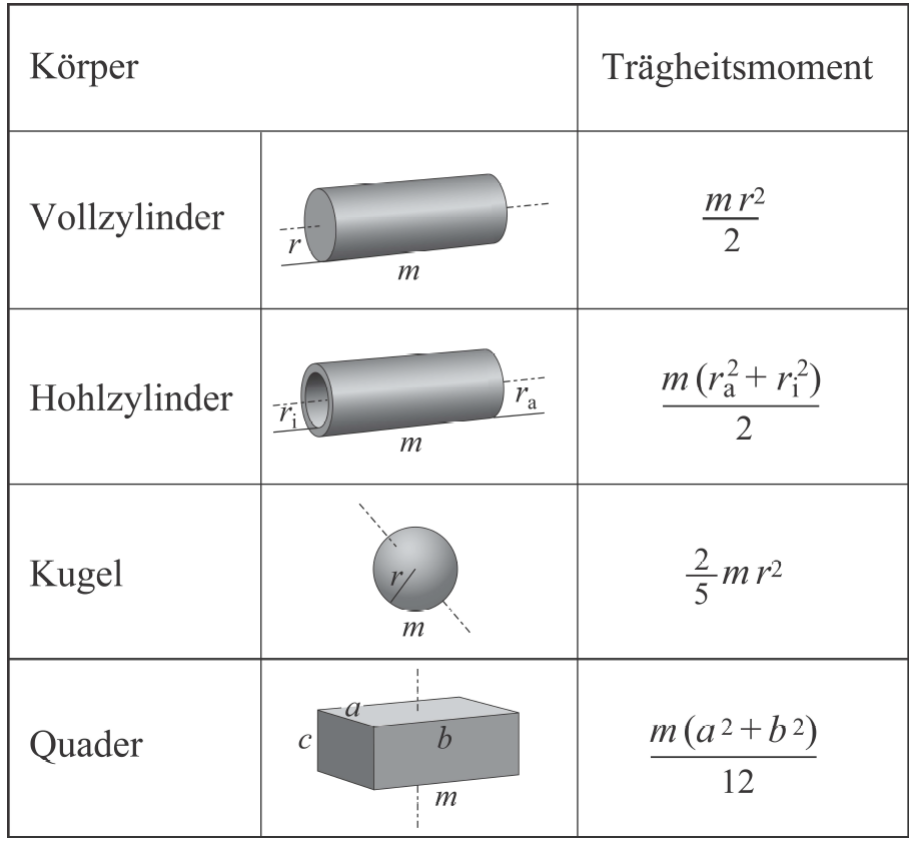
\includegraphics[width=0.75\linewidth]{images/Physik_1-Mechanik.png}
    \begin{tabular}{|c|c|c|} \hline
        \multicolumn{2}{|l|}{\textbf{Körper}} & \textbf{Trägheitsmoment} \\ \hline
        & \multirow{5}{8em}{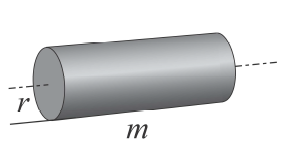
\includegraphics[width=0.9\linewidth]{images/massentraegheitsmomente-vollz.png}} & \\
        Vollzylinder / & & \\
        & & $ \dfrac{m r^2}{2} $\\
        Scheibe & & \\
        & & \\ \hline
        & \multirow{5}{8em}{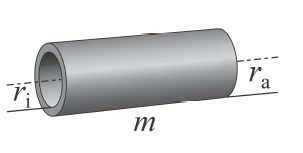
\includegraphics[width=0.9\linewidth]{images/massentraegheitsmomente-hohlz.png}} & \\
        & & \\
        Hohlzylinder & & $ \dfrac{m (r^2_a  + r^2_i)}{2} $\\
        & & \\
        & & \\ \hline
        & \multirow{5}{8em}{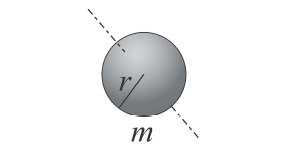
\includegraphics[width=0.9\linewidth]{images/massentraegheitsmomente-kugel.png}} & \\
        & & \\
        Kugel & & $ \dfrac{2}{5} m r^2 $\\
        & & \\
        & & \\ \hline
        & \multirow{5}{8em}{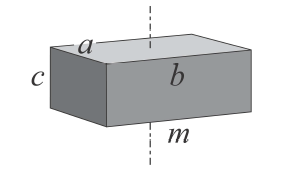
\includegraphics[width=0.9\linewidth]{images/massentraegheitsmomente-quader.png}} & \\
        & & \\
        Quader & & $ \dfrac{m (a^2  + b^2)}{12} $\\
        & & \\
        & & \\ \hline
        & \multirow{5}{8em}{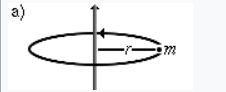
\includegraphics[width=0.9\linewidth]{images/J_massepunkt.png}} & \\
        & & \\
        Massenpunkt & & $ m r^2 $\\
        & & \\
        & & \\ \hline
        & \multirow{5}{8em}{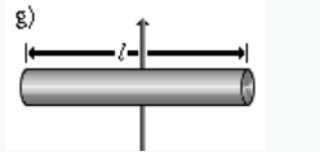
\includegraphics[width=0.9\linewidth]{images/J_duenner_stab_mitte.png}} & \\
        & & \\
        Dünner Stab & & $ \dfrac{1}{12}ml^2 $\\
        & & \\
        & & \\ \hline
    \end{tabular}

\subsection{Vor- und Nachteile Elektroenergie}
    \begin{minipage}[t]{0.49\columnwidth}
        \textbf{Vorteile}
        \begin{itemize}
            \item einfach zu verteilen
            \item beliebig klein dosierbar
            \item gut regulierbar
            \item Einfach in andere Energieformen wandelbar
            \item problemlos und sauber in der Anwendung (keine Emissionen)
            \item Vielfältig einsetzbar
        \end{itemize}
    \end{minipage}%
    \hfill
    \begin{minipage}[t]{0.49\columnwidth}
        \textbf{Nachteile}
        \begin{itemize}
            \item leitungsgebunden
            \item Gleichzeitigkeit von Erzeugung \& Bedarf
            \item nicht direkt aus der Natur gewinnbar
            \item Speicherung ist aufwendig
        \end{itemize}
    \end{minipage}

% \textbf{Vorteile}\\
% \begin{itemize}
%     \item einfach zu verteilen
%     \item beliebig klein dosierbar
%     \item gut regulierbar
%     \item Einfach in andere Energieformen wandelbar
%     \item problemlos und sauber in der Anwendung (keine Emissionen)
%     \item Vielfältig einsetzbar
% \end{itemize}

% \textbf{Nachteile}\\
% \begin{itemize}
%     \item leitungsgebunden
%     \item Gleichzeitigkeit von Erzeugung und Bedarf
%     \item kann nicht direkt aus der Natur gewonnen werden
%     \item Speicherung ist aufwendig
% \end{itemize}

\subsection{Anteil Elektrische Energie}
In der Schweiz beträgt der Anteil Elektrischer Energie bei rund bei rund 25\% bis 30\% des gesamten Endenergieverbrauchs.

% \newcolumn
\subsection{Leistung}

\subsubsection{Rotationsleistung $P_{\text{rot}}$}
$\boxed{P = M \cdot \omega}$ \quad $\boxed{P = M \cdot 2 \cdot \pi \cdot f }$ \quad $\boxed{P = \frac{M \cdot 2 \cdot \pi \cdot n}{60} }$

\vspace{0.15cm}

\renewcommand{\arraystretch}{1.2}
\begin{tabular}{@{} l p {3.5cm} l @{}}
    $[P_{\text{rot}}]$ & Rotationsleistung        \dotfill & $\mathrm{W = \frac{J}{s} = \frac{Nm}{s}}$ \\
    $[M]$              & Drehmoment               \dotfill & $\mathrm{Nm}$ \\
    $[\omega]$         & Winkelgeschwindigkeit    \dotfill & $\mathrm{\frac{rad}{s}}$ \\
    $[f]$              & Drehfrequenz             \dotfill & $\mathrm{Hz = \frac{1}{s}}$ \\
    $[n]$              & Umdrehungen pro Minute   \dotfill & $\mathrm{\frac{1}{min} = \frac{U}{min}}$ \\
\end{tabular}

\subsubsection{Thermische Leistung $P_{\text{th}}$}
$\boxed{P_{\text{th}} = \dot{m} \cdot c \cdot \Delta \vartheta}$ \quad $\boxed{\dot{m} = \rho \cdot \dot{V} }$

\vspace{0.15cm}

\renewcommand{\arraystretch}{1.2}
\begin{tabular}{@{} l p {3.5cm} l @{}}
    $[P_{\text{th}}]$       & Thermische Leistung           \dotfill & $\mathrm{W = \frac{J}{s}}$ \\
    $[\dot{m}]$             & Massenstrom                   \dotfill & $\mathrm{\frac{kg}{s}}$ \\
    $[c]$                   & Spezifische Wärmekapazität    \dotfill & $\mathrm{\frac{J}{kg \cdot K}}$ \\
    $[\Delta \vartheta]$    & Temperaturdifferenz           \dotfill & $\mathrm{K}$ oder $^\circ\mathrm{C}$ \\
    $[\rho]$                & Dichte                        \dotfill & $\mathrm{\frac{kg}{m^3}}$ \\
    $[\dot{V}]$             & Volumenstrom                  \dotfill & $\mathrm{\frac{m^3}{s}}$ \\
\end{tabular}

\subsubsection{Transmissions-Wärmeverlustleistung $P_{\text{VW}}$}
$\boxed{P_{\text{VW}} = U \cdot A \cdot \Delta \vartheta}$

\vspace{0.15cm}

\renewcommand{\arraystretch}{1.2}
\begin{tabular}{@{} l p {3.5cm} l @{}}
    $[P_{\text{VW}}]$           & Wärmeverlustleistung          \dotfill & $\mathrm{W = \frac{J}{s}}$ \\
    $[U]$                       & Wärmedurchgangskoeffizient    \dotfill & $\mathrm{\frac{W}{m^2 \cdot K}}$ \\
    $[A]$                       & Fläche                        \dotfill & $\mathrm{m^2}$ \\
    $[\Delta \vartheta]$        & Temperaturdifferenz           \dotfill & $\mathrm{K}$ \\
\end{tabular}

\subsubsection{Mechanische Leistung $P_v$}
$\boxed{P_v = F \cdot v}$ \quad $\boxed{F = m \cdot g}$

\vspace{0.15cm}

\renewcommand{\arraystretch}{1.2}
\begin{tabular}{@{} l p {3.5cm} l @{}}
    $[P_v]$   & Mechanische Leistung   \dotfill & $\mathrm{W = \frac{J}{s} = \frac{Nm}{s}}$ \\
    $[F]$     & Kraft                  \dotfill & $\mathrm{N = kg \cdot \frac{m}{s^2}}$ \\
    $[m]$     & Masse                  \dotfill & $\mathrm{kg}$ \\
    $[g]$     & Erdbeschleunigung      \dotfill & $\mathrm{\frac{m}{s^2}}$ \\
    $[v]$     & Geschwindigkeit        \dotfill & $\mathrm{\frac{m}{s}}$ \\
\end{tabular}



\subsubsection{Leistung der Solaranlage $P_{\text{PV}}$}
$\boxed{P_{\text{PV}} = \eta \cdot A \cdot E}$

\vspace{0.15cm}

\renewcommand{\arraystretch}{1.2}
\begin{tabular}{@{} l p {3.5cm} l @{}}
    $[P_{\text{PV}}]$    & Elektrische Leistung         \dotfill & $\mathrm{W = \frac{J}{s}}$ \\
    $[\eta]$             & Wirkungsgrad                 \dotfill & $-$ \\
    $[A]$                & Fläche der Solaranlage       \dotfill & $\mathrm{m^2}$ \\
    $[E]$                & Einstrahlung                 \dotfill & $\mathrm{\frac{W}{m^2}}$ \\
\end{tabular}



\subsubsection{Leistung eines Wasserkraftwerks $P$}
$\boxed{P = \eta \cdot \rho \cdot g \cdot \dot{V} \cdot h}$

\vspace{0.15cm}

\renewcommand{\arraystretch}{1.2}
\begin{tabular}{@{} l p {3.5cm} l @{}}
    $[P]$         & Elektrische Leistung          \dotfill & $\mathrm{W = \frac{J}{s}}$ \\
    $[\eta]$      & Wirkungsgrad                  \dotfill & $-$ \\
    $[\rho]$      & Dichte                        \dotfill & $\mathrm{\frac{kg}{m^3}}$ \\
    $[g]$         & Erdbeschleunigung             \dotfill & $\mathrm{\frac{m}{s^2}}$ \\
    $[\dot{V}]$   & Volumenstrom                  \dotfill & $\mathrm{\frac{m^3}{s}}$ \\
    $[h]$         & Höhendifferenz                \dotfill & $\mathrm{m}$ \\
\end{tabular}



\subsubsection{Verminderung des Wasserstands in einem Stausee $\Delta h$}
$\boxed{\Delta h = \frac{V}{A_\mathrm{Stausee}} = \frac{Q \cdot t}{A_\mathrm{Stausee}}}$

\renewcommand{\arraystretch}{1.2}
\begin{tabular}{@{} l p{6.5cm} l @{}}
    $[h]$               & Wasserstandssenkung im Stausee \dotfill & $\mathrm{m}$ \\
    $[V]$               & Entnommenes Wasservolumen \dotfill & $\mathrm{m^3}$ \\
    $[A_\mathrm{Stausee}]$ & Oberfläche des Stausees \dotfill & $\mathrm{m^2}$ \\
    $[Q]$               & Volumenstrom (z.\,B. Turbinenstrom) \dotfill & $\frac{\mathrm{m^3}}{\mathrm{s}}$ \\
    $[t]$               & Zeitdauer der Entnahme \dotfill & $\mathrm{s}$ \\
\end{tabular}



\subsubsection{Drehstrom-Leistungsberechnung $P_{\circlearrowleft}$}
$\boxed{P_{\circlearrowleft} = \sqrt{3} \cdot U \cdot I \cdot \cos(\varphi)}$

\vspace{0.15cm}

\renewcommand{\arraystretch}{1.2}
\begin{tabular}{@{} l p {3.5cm} l @{}}
    $[P_{\circlearrowleft}]$  & Wirkleistung              \dotfill & $\mathrm{W = \frac{J}{s}}$ \\
    $[U]$                     & Verkettete Spannung       \dotfill & $\mathrm{V}$ \\
    $[I]$                     & Stromstärke               \dotfill & $\mathrm{A}$ \\
    $[\cos(\varphi)]$         & Leistungsfaktor           \dotfill & $-$ \\
\end{tabular}

\subsection{Schweizer Strom-Mix}
\begin{tabular}{|c|l|}
    \hline
    38.1 \% & Kernkraft \\ \hline
    32.3 \% & Speicherkraftwerke \\ \hline
    24.2 \% & Laufkraftwerke \\ \hline
    5.4 \%  & konventionell-thermische Kraftwerke \\ \hline
    1.52 \% & Kehrichtverbrennungsanlagen \\ \hline
    0.29 \% & Biomasse \\ \hline
    0.19 \% & Abwasserreinigungsanlagen \\ \hline
    0.13 \% & Photovoltaik \\ \hline
    0.06 \% & Windkraft \\ \hline
\end{tabular}

\subsection{Investitions- und Kostenrechnung}

\subsubsection{Annuitätsfaktor $A$}
$\boxed{A = \frac{(1 + i)^n \cdot i}{(1 + i)^n - 1}}$

\vspace{0.15cm}

\renewcommand{\arraystretch}{1.2} % Erhöht Zeilenhöhe für bessere Lesbarkeit
\begin{tabular}{@{} l p {3.5cm} l @{}}
    $[A]$       & Annuitätsfaktor           \dotfill & $1$ \\
    $[i]$       & Zinsen                    \dotfill & $1$ \\
    $[n]$       & Anzahl Jahre Laufzeit     \dotfill & $1$ \\
\end{tabular}


\subsubsection{Kapitalkosten $K_{\text{K}}$}
$\boxed{K_{\text{K}} = A \cdot I}$

\vspace{0.15cm}

\renewcommand{\arraystretch}{1.2} % Erhöht Zeilenhöhe für bessere Lesbarkeit
\begin{tabular}{@{} l p {3.5cm} l @{}}
    $[K_{\text{K}}]$    & Kapitalkosten     \dotfill & CHF oder € \\
    $[A]$               & Annuitätsfaktor   \dotfill & $1$ \\
    $[I]$               & Investitionen     \dotfill & CHF oder € \\
\end{tabular}


\subsubsection{Unterhaltskosten $K_{\text{U}}$}
$\boxed{K_{\text{U}} = p_{\text{U}} \cdot I}$

\vspace{0.15cm}

\renewcommand{\arraystretch}{1.2} % Erhöht Zeilenhöhe für bessere Lesbarkeit
\begin{tabular}{@{} l p {3.5cm} l @{}}
    $[K_{\text{U}}]$    & Unterhaltskosten              \dotfill & CHF oder € \\
    $[p_{\text{U}}]$    & Unterhaltskosten-Prozentsatz  \dotfill & $1$ \\
    $[I]$               & Investitionen                 \dotfill & CHF oder € \\
\end{tabular}


\subsubsection{Fix-Kosten $K_{\text{Fix}}$}
$\boxed{K_{\text{Fix}} = K_{\text{K}} + K_{\text{U}} = (A + p_{\text{U}}) \cdot I}$

\vspace{0.15cm}

\renewcommand{\arraystretch}{1.2} % Erhöht Zeilenhöhe für bessere Lesbarkeit
\begin{tabular}{@{} l p {3.5cm} l @{}}
    $[K_{\text{Fix}}]$    & Fix-Kosten              \dotfill & CHF oder € \\
\end{tabular}


\subsubsection{Erlös oder Deckungsbeitrag $E$}
$\boxed{E = t_{\text{VL}} \cdot C \cdot P}$

\vspace{0.15cm}

\renewcommand{\arraystretch}{1.2} % Erhöht Zeilenhöhe für bessere Lesbarkeit
\begin{tabular}{@{} l p {3.5cm} l @{}}
    $[E]$               & Erlös             \dotfill & CHF oder € \\
    $[t_{\text{VL}}]$   & Volllaststunden   \dotfill & $\mathrm{h}$ \\
    $[C]$               & Grenzkosten       \dotfill & $\frac{\text{CHF}}{\text{MWh}}$ oder $\frac{\text{€}}{\text{MWh}}$ \\
    $[P]$               & Leistung          \dotfill & $\mathrm{W = \frac{Nm}{s} = \frac{J}{s}}$ \\
\end{tabular}


\subsubsection{Ergebnis (Gewinn oder Verlust) $G$}
$\boxed{G = E - K_{\text{Fix}} - K_{\text{Var}}}$

\subsubsection{Variable Kosten $K_{\text{V}}$}

\vspace{0.15cm}

\renewcommand{\arraystretch}{1.2} % Erhöht Zeilenhöhe für bessere Lesbarkeit
\begin{tabular}{@{} l p {3.5cm} l @{}}
    $[G]$               & Ergebnis        \dotfill & CHF oder € \\
    $[E]$               & Erlös           \dotfill & CHF oder € \\
    $[K_{\text{Fix}}]$  & Fix-Kosten      \dotfill & CHF oder € \\
    $[K_{\text{Var}}]$  & Variable Kosten \dotfill & CHF oder € \\
\end{tabular}

\subsection{Kraftwerke im Vergleich}
\begin{tabular}{|l|l|l|l|}
\hline
Kraftwerksart & $P_{el}$/MW & $\eta$/\% & $W/P_{el}$ kWh/kW \\
\hline
Kernkraftwerke & 500...1300 & 33...37 & 1,3...4 \\
Dampfkraftwerke & 100...1000 & 35...43 & 0,5...1,1 \\
Wasserkraftwerke & 10...820 & 85...95 & 0,2...0,4 \\
GuD-Kraftwerke & 100...300 & 50...58 & 0,8...1,1 \\
Gasturbinenkraftwerke & 10...265 & 34...39,5 & 0,2...0,5 \\
BHKW & 0,05...20 & 32...40 & 0,8...1,3 \\
Windkraftanlagen & 0,01...5 & 20...30 & 7 $\cdot 10^3$...20 $\cdot 10^3$ \\
Solarkraftwerke & ...80 & 10...14 & 5...10 \\
PV-Kraftwerke & ...7 & 6...12 & 7 $\cdot 10^3$...20 $\cdot 10^3$ \\
\hline
\end{tabular}     % done
        \section{Wasserdargebot für Wasserkraft}

\subsection{Abflussganglinie}
    \begin{minipage}[t]{0.4\columnwidth}
        Abfluss $Q_b$ in \unit{\cubic\metre\per\second} während eines Jahres (365 Tage)
    \end{minipage}%
    \hfill
    \begin{minipage}[c]{0.58\columnwidth}
        \begin{center}
            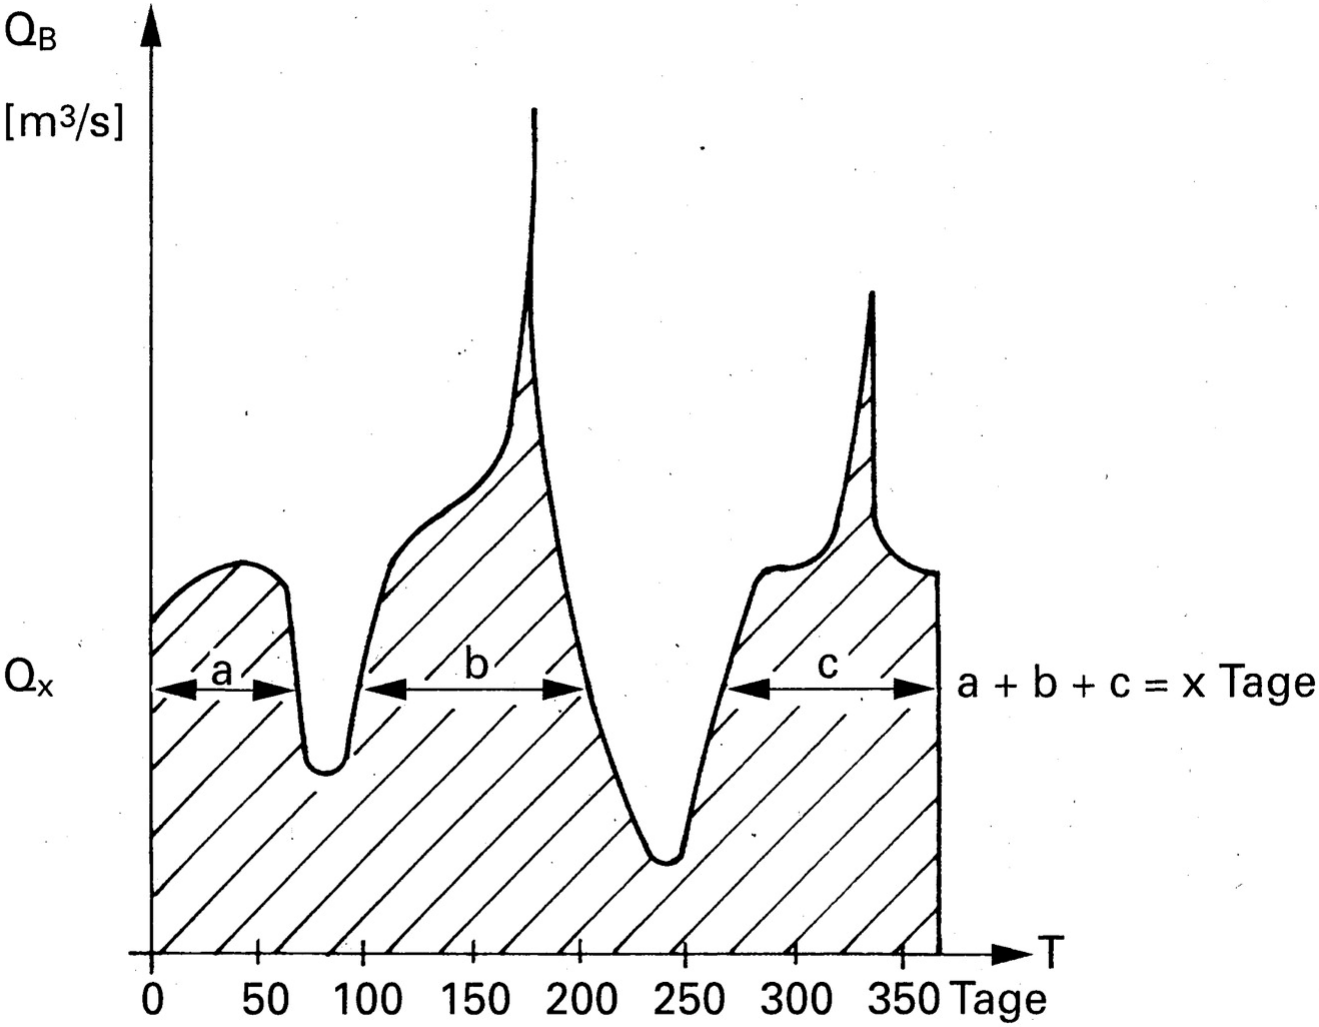
\includegraphics[width=0.95\textwidth, align=c]{images/Abflussganglinie.png}
        \end{center}
    \end{minipage}

\subsection{Abflussdauerkurve}
    \begin{minipage}[t]{0.4\columnwidth}
        Abfluss $Q_b$ in \unit{\cubic\metre\per\second} während eines Jahres (365 Tage), sortiert der Grösse nach

        \medskip

        \textbf{Abfluss ist an 275 Tagen mindestens $Q_x$}
    \end{minipage}%
    \hfill
    \begin{minipage}[c]{0.48\columnwidth}
        \begin{center}
            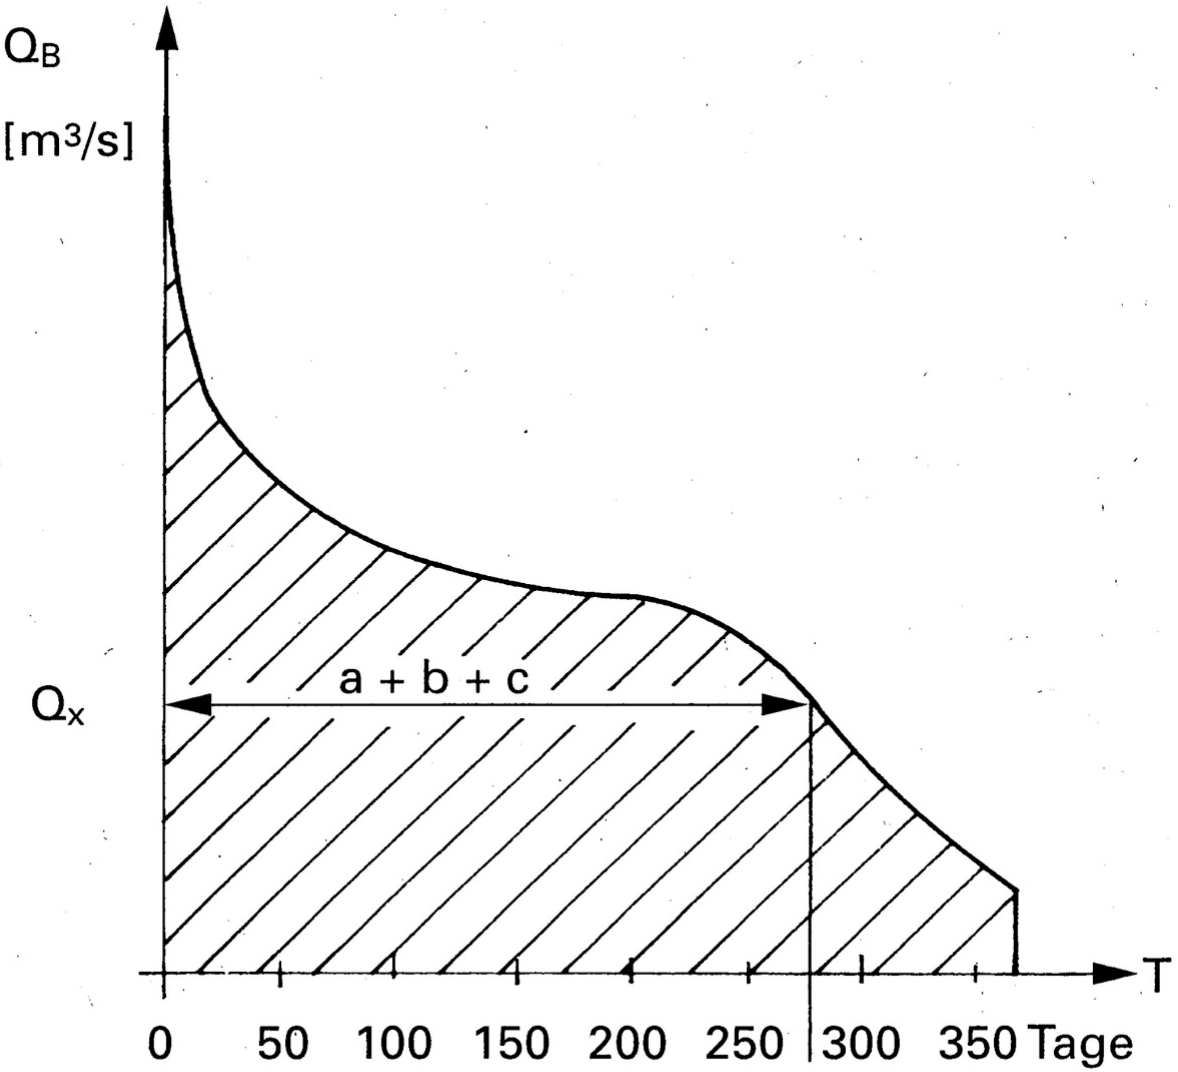
\includegraphics[width=0.95\textwidth, align=c]{images/Abflussdauerkurve.png}
        \end{center}
    \end{minipage}

\subsection{Nutzwassermenge}
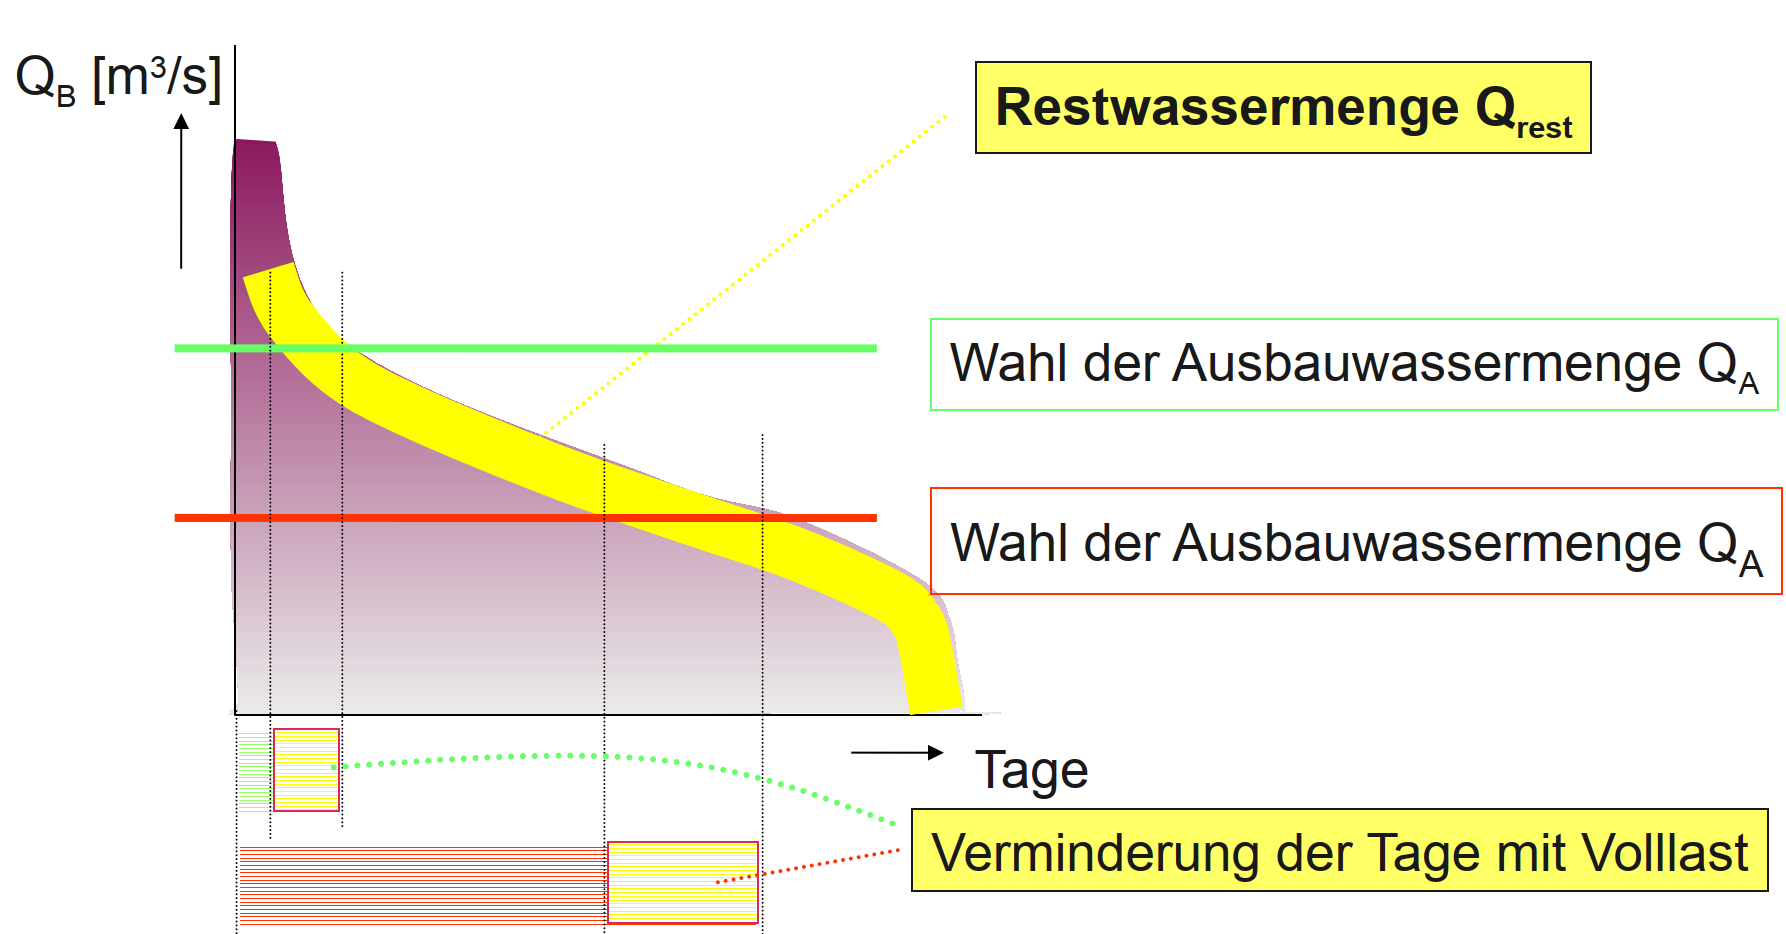
\includegraphics[width=0.8\columnwidth, align=c]{images/Nutzwassermenge.png}

\vspace{0.1cm}

$\boxed{Q_{Nutz} = Q_B - Q_{Rest}}$

\vspace{0.1cm}

\renewcommand{\arraystretch}{1.2} % Erhöht Zeilenhöhe für bessere Lesbarkeit
\begin{tabular}{@{} l p {6cm} l @{}}
    $[Q_{Nutz}]$    & Nutzwassermenge   \dotfill & \unit{\cubic\metre\per\second} \\
    $[Q_B]$         & Abflussmenge      \dotfill & \unit{\cubic\metre\per\second} \\
    $[Q_{Rest}]$    & Restwassermenge   \dotfill & \unit{\cubic\metre\per\second} \\
\end{tabular}

\subsubsection{Mindest Restwassermenge $Q_{\mathrm{Rest}}$}

$Q_{\mathrm{Rest}}$ muss aufgrund von ökologischen Mindestanforderungen \textbf{immer} gewährleistet sein.

\begin{tabular}{>{\raggedright}p{6.5cm} r}
\toprule
\textbf{Abflussmenge $Q_{347}$} & \textbf{Restwassermenge} \\
\midrule
bis 60 l/s Abflussmenge $Q_{347}$ & 50 l/s \\
$\to$ pro weitere 10 l/s Abflussmenge $Q_{347}$ & 8 l/s mehr \\
\addlinespace
bis 160 l/s Abflussmenge $Q_{347}$ & 130 l/s \\
$\to$ pro weitere 10 l/s Abflussmenge $Q_{347}$ & 4{,}4 l/s mehr \\
\addlinespace
bis 500 l/s Abflussmenge $Q_{347}$ & 280 l/s \\
$\to$ pro weitere 100 l/s Abflussmenge $Q_{347}$ & 31 l/s mehr \\
\addlinespace
bis 2500 l/s Abflussmenge $Q_{347}$ & 900 l/s \\
$\to$ pro weitere 100 l/s Abflussmenge $Q_{347}$ & 21{,}3 l/s mehr \\
\addlinespace
bis 10\,000 l/s Abflussmenge $Q_{347}$ & 2\,500 l/s \\
$\to$ pro weitere 1\,000 l/s Abflussmenge $Q_{347}$ & 150 l/s mehr \\
\addlinespace
ab 60\,000 l/s Abflussmenge $Q_{347}$ & 10\,000 l/s \\
\bottomrule
\end{tabular}

\subsection{Triebwassersystem}
Ein Triebwassersystem führt das Wasser vom Speicher zur Turbine eines Wasserkraftwerks. 
Es beinhaltet die Leitungswege wie Stollen und Druckleitungen. 
Verluste darin sind bei Speicherkraftwerken bedeutsam, bei Laufwasserkraftwerken jedoch meist vernachlässigbar. % done
        \input{sections/10_Wasserkraft.tex}  % done
        \section{Talsperren}
\subsection{Bogenstaumauer}
    \begin{minipage}[c]{0.38\columnwidth}
        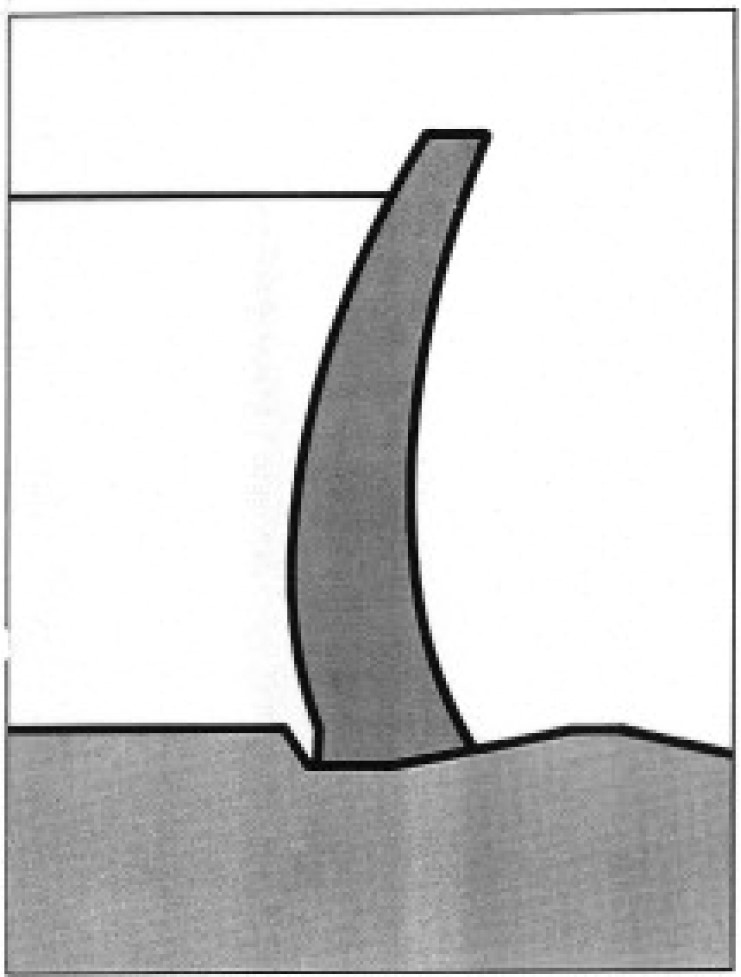
\includegraphics[width=0.85\columnwidth, align=c]{images/Talsperre_1.jpg}
    \end{minipage}
    \hfill
    \begin{minipage}[t]{0.58\columnwidth}
        \begin{itemize}
        \item Beton
        \item Schlank
        \item Kraft wird links und rechts in den Hang geleitet (Gewölbewirkung)
        \item Beispiel: Verzasca Damm (Tessin)
        \end{itemize}
    \end{minipage}

\subsection{Gewichtsstaumauer}
    \begin{minipage}[c]{0.38\columnwidth}
        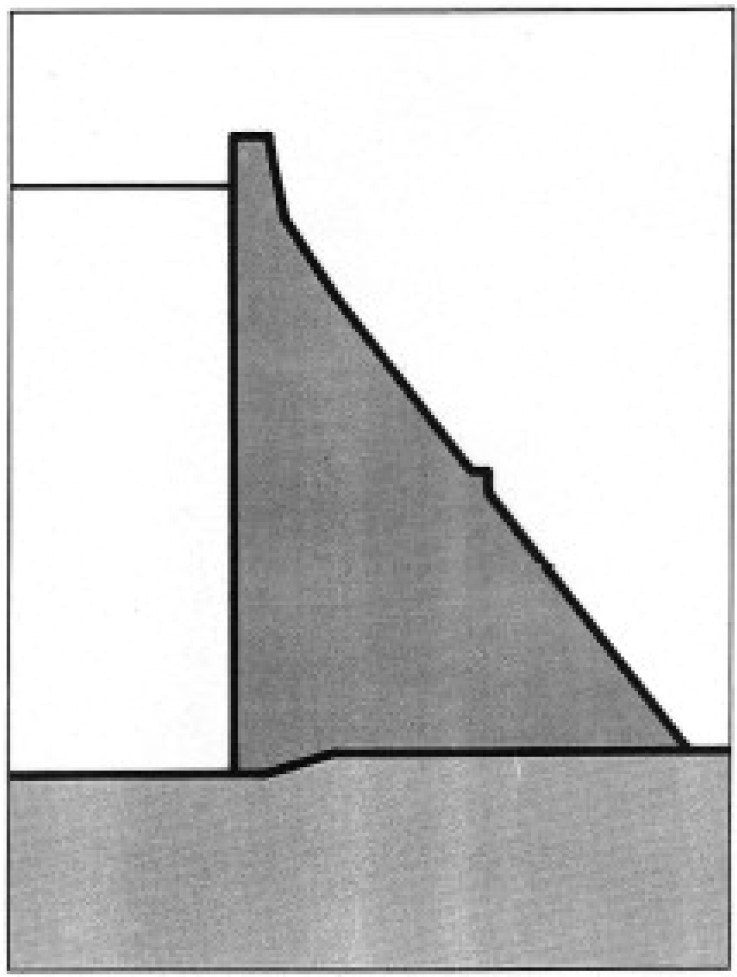
\includegraphics[width=0.85\columnwidth, align=c]{images/Talsperre_2.jpg}
    \end{minipage}
    \hfill
    \begin{minipage}[c]{0.58\columnwidth}
        \begin{itemize}
        \item Beton oder Mauerwerk
        \item Hohes Eigengewicht
        \item Kraft wird durch Eigengewicht gehalten
        \item Beispiel: Grande Dixence (Wallis) Höchste Gewichtsstaumauer der Welt
        \end{itemize}
    \end{minipage}

\subsection{Staudamm}
    \begin{minipage}[c]{0.45\columnwidth}
        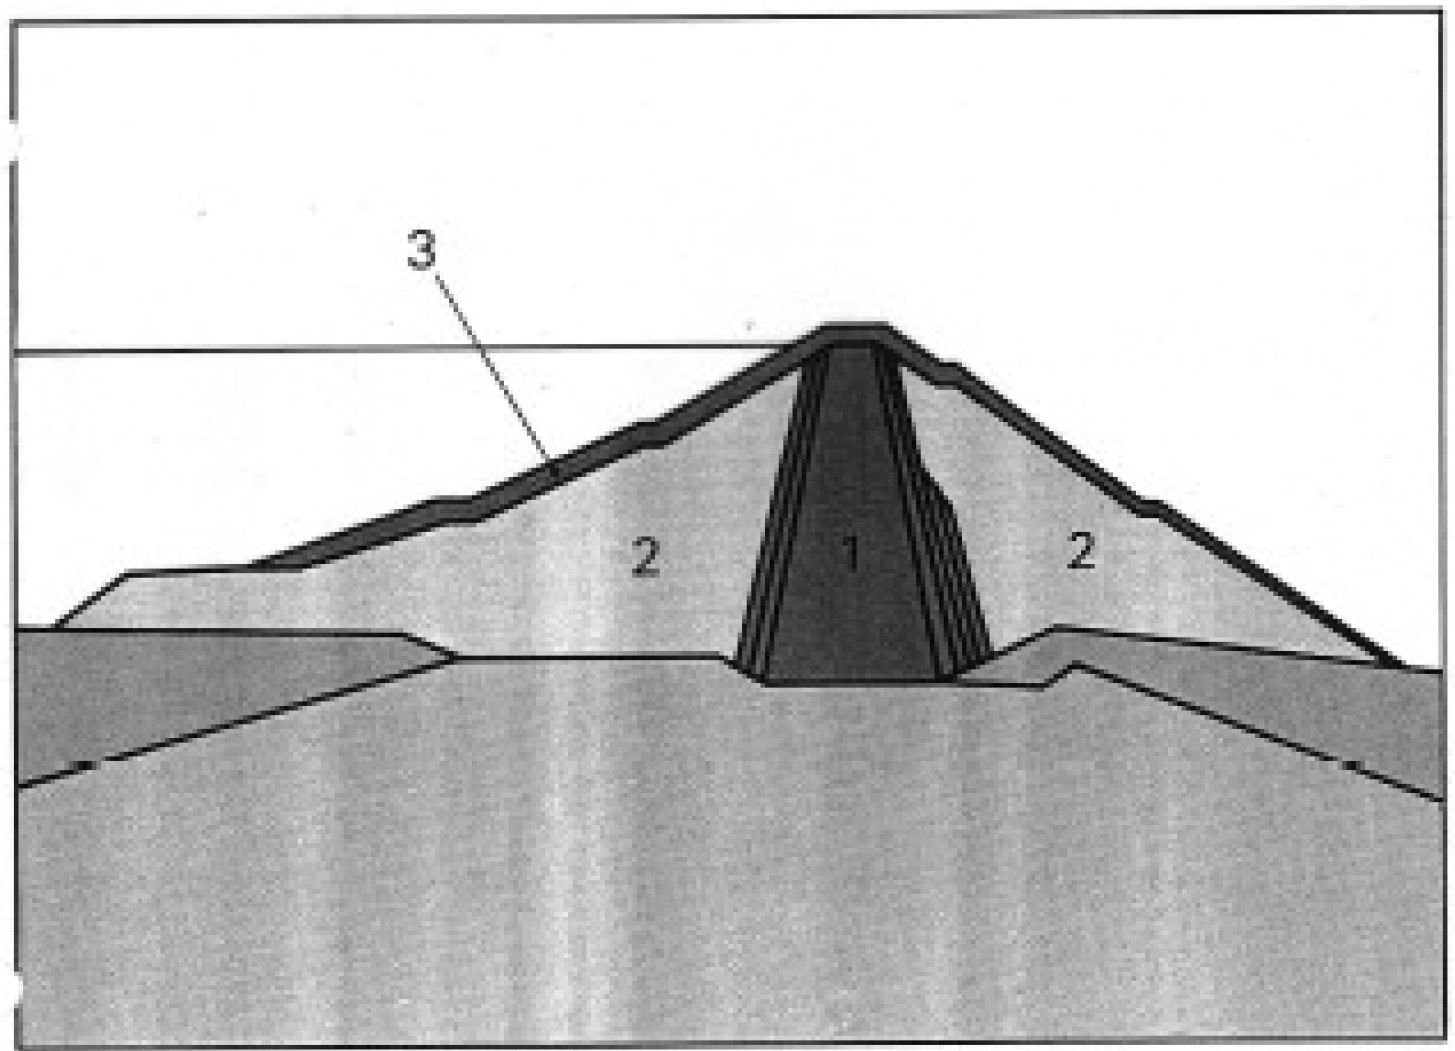
\includegraphics[width=0.85\columnwidth, align=c]{images/Talsperre_3.jpg}
    \end{minipage}
    \hfill
    \begin{minipage}[c]{0.54\columnwidth}
       \begin{enumerate}
            \item Kern 
            \item Stützkörper
            \item Schutzschicht
        \end{enumerate}

        \vspace{0.15cm}

        \begin{itemize}
            \item Aufgeschüttet
            \item Flacher Böschungswinkel
            \item Steinschüttung unterschiedlicher Korngrösse
            \item Beispiel: Stausee Mattmark (Wallis) (Höchster Erdschüttdamm der Welt)
        \end{itemize}
    \end{minipage}

\section{Synchronmaschinen}
\subsection{Typen}
\begin{minipage}[c]{0.49\columnwidth}
    \begin{center}
        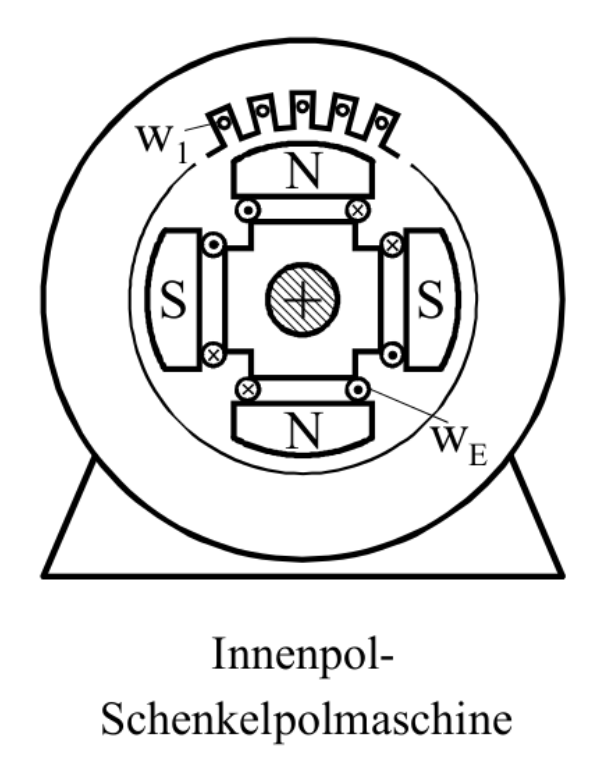
\includegraphics[width=0.9\linewidth]{images/Schenkelpolmaschine.png}

        \begin{tabular}{c}
            Zwei oder vier Pole\\
            $n=3000$ oder $5000\, \mathrm{U/min}$\\
            Sinusförmiges Magnetfeld
        \end{tabular}
    \end{center}
\end{minipage}
\begin{minipage}[c]{0.49\columnwidth}
    \begin{center}
        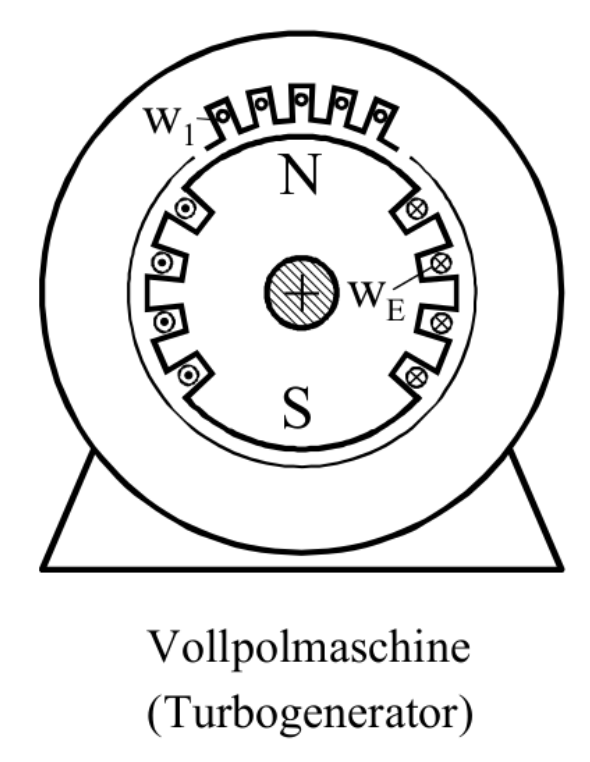
\includegraphics[width=0.9\linewidth]{images/Vollpolmaschine.png}

        \begin{tabular}{c}
            $>80$ Einzelpole möglich\\
            Langsam drehend, gut für Wasserkraft\\
            Eher rechteckiges Magnetfeld
        \end{tabular}
    \end{center}
\end{minipage}

\subsection{Betriebsarten Generator}
\subsubsection{Leerlauf}
\begin{minipage}[c]{0.3\columnwidth}
    $\boxed{U_p = \frac{1}{\sqrt{2}}2\pi f w_1\xi_1\Phi_h}$
\end{minipage}
\hfill
\begin{minipage}[c]{0.69\columnwidth}
    \begin{tabular}{@{} l p{4cm} l @{}}
        $[U_p]$      & Polradspannung \dotfill & $\text{V}$ \\
        $[f]$        & Frequenz = Mech.$f\cdotp$ \dotfill & $\mathrm{Hz}$ \\
        $[w_1\xi_1]$ & Wirk Windungszahl Stator \dotfill& $-$ \\
        $[\Phi_h]$   & Magn. Fluss durch Erregerstrom $I_{\mathrm{E}}$ \dotfill& $\mathrm{Wb}$\\
    \end{tabular}
\end{minipage}

\subsubsection{Generator mit Last}
\begin{minipage}[c]{0.46\columnwidth}
    $\boxed{\underline{U}_1 = \underline{U}_p +\underline{I}_1 \cdot\left(R_1+j(X_h+X_{\sigma1})\right)}$ \\
    $\boxed{X_d = X_h+X_{\sigma1}}$ \\
    $\boxed{\underline{U}_1 = \underline{U}_p +\underline{I}_1 \cdot(R_1+j(X_h+X_{\sigma1}))}$ \\
    $\boxed{\phi = \angle\underline{I}_1 \underline{U}_1} \quad \boxed{\vartheta = \angle\underline{U}_1\underline{U}_p}$ \\
    $\boxed{\underline{I}_1 = j\cdot \frac{\underline{U}_p-\underline{U}_1}{X_d}} \quad \boxed{U_x = j\cdot\underline{I}_1\cdot X_d}$\\
    $\boxed{\underline{I}_1= \frac{S}{3\cdot \underline{U}_1}} \quad \boxed{\frac{I_e}{I_{e0}}=\frac{U_p}{U_1}}$ \\
\end{minipage}
\hfill
\begin{minipage}[c]{0.53\columnwidth}
    \begin{tabular}{@{} l p{3.2cm} l @{}}
    $[U_1]$      & Klemmenspannung \dotfill & $\text{V}$ \\
    $[U_p]$      & Polradspannung \dotfill & $\mathrm{V}$ \\
    $[U_x]$      & Spannung über $X_d$ \dotfill& $\mathrm{V}$\\
    $[I_1]$ & Statorstrom \dotfill& $\mathrm{A}$ \\
    $[X_h]$  & Hauptreaktanz \dotfill& $\mathrm{H}$\\
    $[X_{\sigma1}]$   & Streureaktanz \dotfill& $\mathrm{H}$\\
    $[X_d]$  & Synchronreaktanz \dotfill& $\mathrm{H}$\\
    $[\phi]$  & Phasenverschiebung \dotfill& $\mathrm{rad/^\circ}$\\
    $[\vartheta]$  & Polradwinkel \dotfill& $\mathrm{^\circ}$\\
    $[S]$ & Scheinleistung \dotfill& $\mathrm{VA}$\\
    $[I_e]$ & Nennerregerstrom \dotfill& $\mathrm{A}$\\
    $[I_{e0}]$ & Leerelauferregerstrom \dotfill& $\mathrm{A}$\\
\end{tabular}
\end{minipage}

\begin{center}
    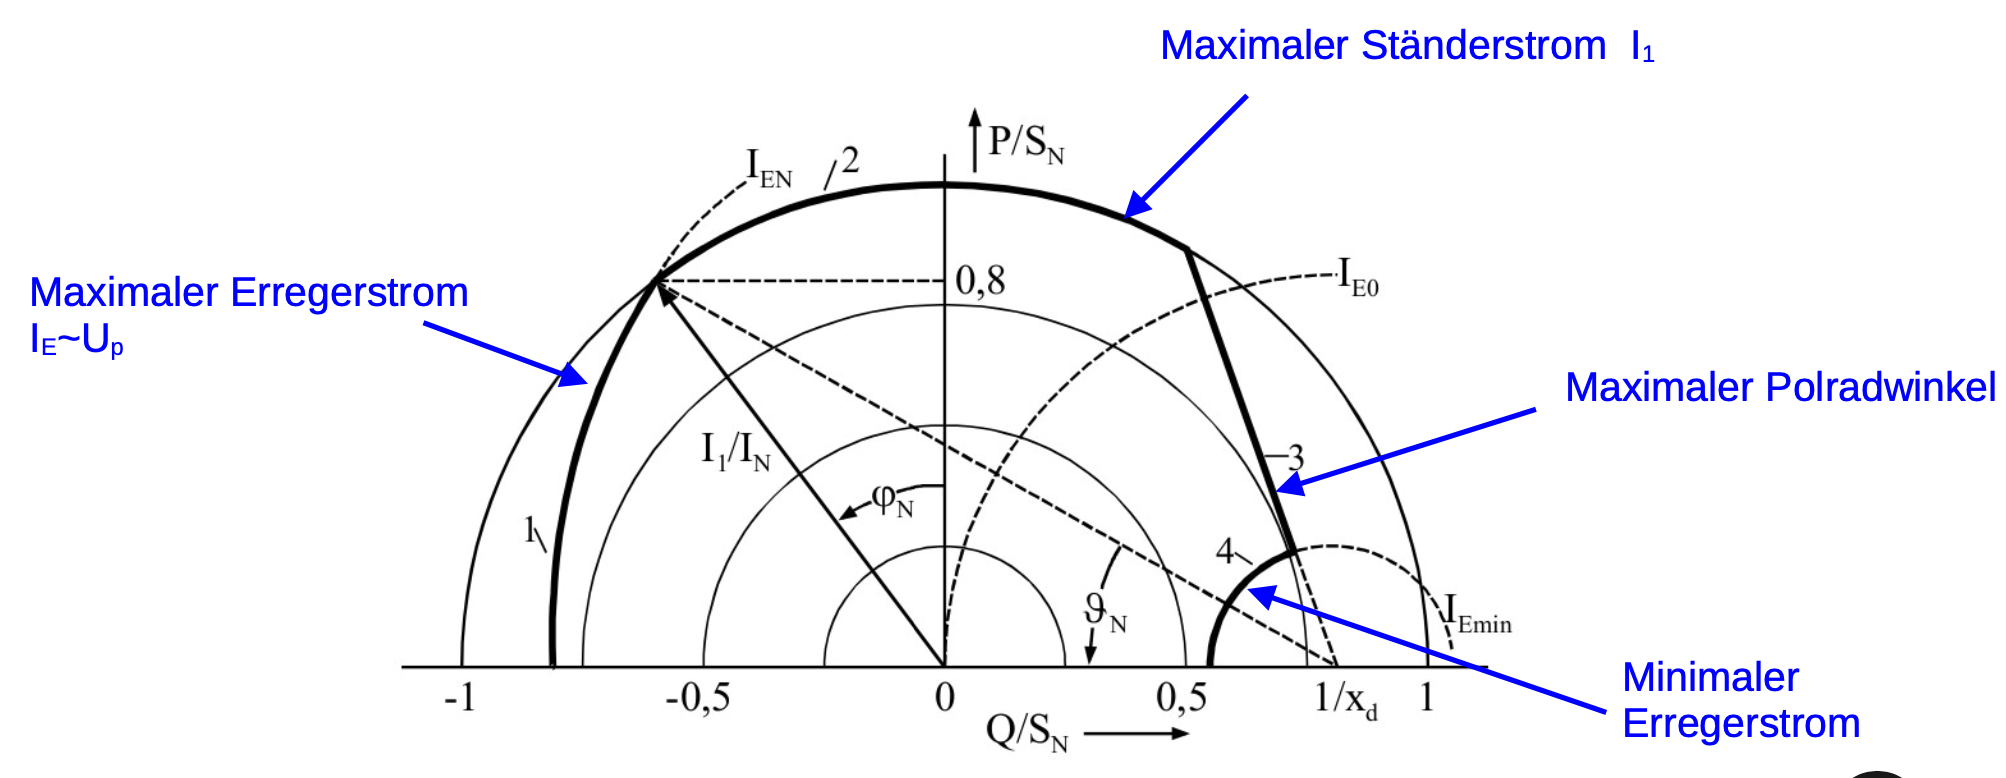
\includegraphics[width=0.9\columnwidth]{images/Leistungsdiagramm.png}
    Leistungsdiagramm
\end{center}

\subsection{Drehmoment, Kippmoment, Stabilitätsgrenze, Leistung}
\begin{minipage}[c]{1\columnwidth}
    \begin{itemize}
        \item Im Normalbetrieb $\vartheta \approx 30^\circ$ (Turbogenerator), $\vartheta = 20 - 25^\circ$ (Schenkelpolmaschine)
        \item Nenndrehmoment etwa halb so gross wie Kippmoment($\sin30^\circ = 1/2$)
        \item Sicherheitsmarge für transiente Vorgänge: $\vartheta$ zwischen $70 - 80^\circ$
    \end{itemize}

\end{minipage}
\begin{minipage}[c]{0.45\columnwidth}
    $\boxed{P_1 = |\underline{U}_1| \cdot |\underline{I}_1|\cdot\cos\phi}$\\
    $\boxed{P_1 = \frac{|\underline{U}_1|}{X_d} \cdot \sin\vartheta}$\\
    $\boxed{P_{tot}= 3\cdot P_1}$
    $\boxed{P_{tot}=P_{mech} = \Omega\cdot M = \frac{\omega}{p} \cdot M}$
    $\boxed{M  = P_{tot} \cdot \frac{p}{\omega} = 3\cdot|\underline{U_1}|\frac{|\underline{U_p}|}{X_d}\sin\vartheta\cdot\frac{p}{\omega}  }$
    $\boxed{M_k  = 3\cdot |\underline{U_1}| \frac{|\underline{U_p}|}{X_d}\frac{p}{\omega}\Rightarrow\vartheta=90^\circ}$
\end{minipage}
\hfill
\begin{minipage}[c]{0.55\columnwidth}
    \begin{tabular}{@{} l p{3.2cm} l @{}}
        $[U_1]$      & Klemmenspannung \dotfill & $\text{V}$ \\
        $[U_p]$      & Polradspannung \dotfill & $\mathrm{V}$ \\
        $[I_1]$ & Statorstrom \dotfill& $\mathrm{A}$ \\
        $[X_d]$  & Synchronreaktanz \dotfill& $\mathrm{H}$\\
        $[\phi]$  & Phasenverschiebung \dotfill& $\mathrm{rad/^\circ}$\\
        $[\vartheta]$  & Polradwinkel \dotfill& $\mathrm{^\circ}$\\
        $[P]$  & Leisung an $\mathrm{L_1}$ \dotfill& $\mathrm{W}$\\
        $[P_{tot}]$  & Gesamtleisung \dotfill& $\mathrm{W}$\\
        $[P_{mech}]$  & Mechanische Leistung \dotfill& $\mathrm{W}$\\
        $[\Omega]$  & Kreisfrequenz Rotor \dotfill& $\mathrm{rad/s}$\\
        $[\omega]$  & Kreisfrequenz \dotfill& $\mathrm{rad/s}$\\
        $[p]$  & Polpaarzahl \dotfill& $-$\\
        $[M]$  & Drehmoment \dotfill& $\mathrm{Nm}$\\
        $[M_k]$  & Kippmoment $|\vartheta| > 90^\circ$ \dotfill& $\mathrm{Nm}$\\
    \end{tabular}
\end{minipage}

\subsection{Zeigerdiagramm}
\begin{minipage}[t]{0.49\columnwidth}
    \begin{itemize}
        \item Verbraucherzählpfeilsystem: Beim Generatorbetrieb zeigt $I_1$ in die andere Richtung als $U_1$
        \item $U_x = j\cdot I_1\cdot X_d$ ist die Spannung an der Synchronreaktanz (immer senkrecht zu $I_1$)
        \item Erregerstrom $I_E$ immer senkrecht zu $U_p$
    \end{itemize}
\end{minipage}
\hfill
\begin{minipage}[t]{0.49\columnwidth}
    \begin{itemize}
        \item Sind $U_1$, $I_1$ und $X_d$ gegeben können $U_x$, $U_p$ und $\vartheta$ konstruktiv bestimmt werden.
        \item Polradwinkel $\vartheta>0$: Motorbetrieb, $\vartheta<0$:Generatorbetrieb
        \item Polradwinkel wächst mit Belastung
        \item $\phi>0$: Übererregt, $\phi<0$: Untererregt
    \end{itemize}
    \vfill
\end{minipage}

\begin{center}
    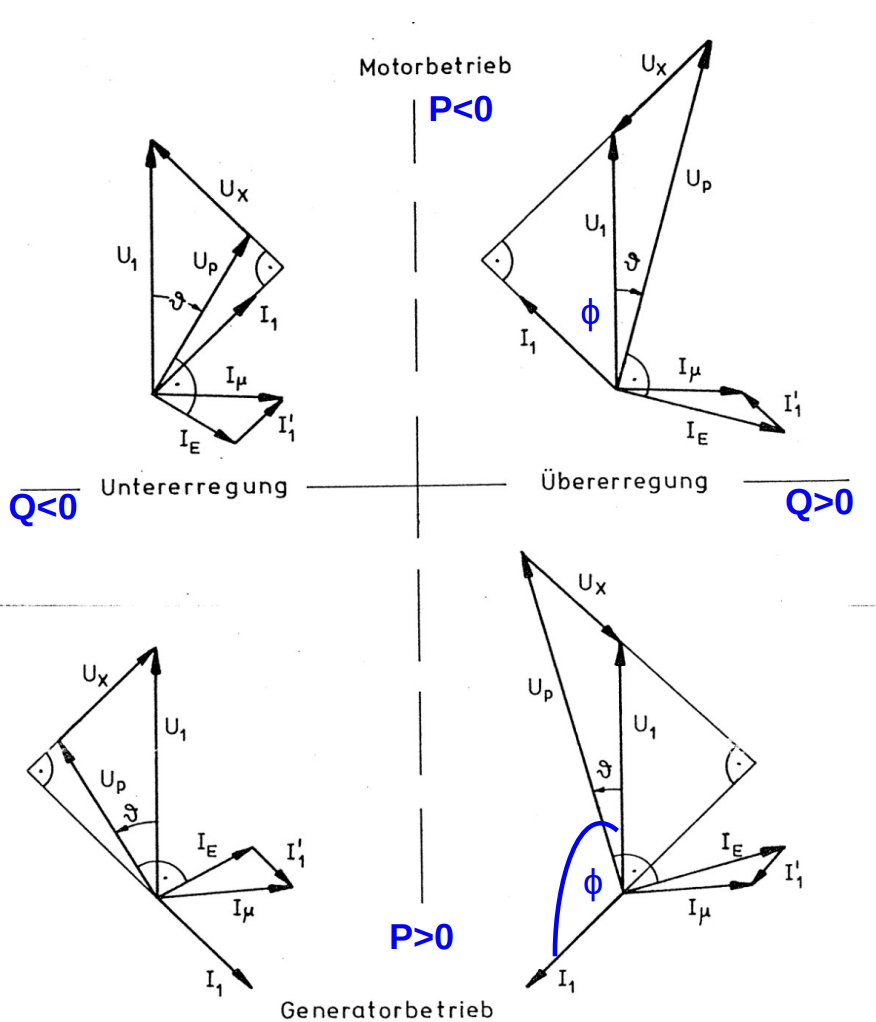
\includegraphics[width=0.85\columnwidth]{images/Maschinen.png}
\end{center}

\begin{tabular}{l l l l l l}
    $[U_{n}]$  & Verkettete Spannung & $\mathrm{V}$ &   
    $[U_{1}]$  & Strangspannung $U_{1} = \frac{U_n}{\sqrt{3}}$   & $\mathrm{V}$ \\  
    $[X_d]$  & Synchronreaktanz  & $\mathrm{\Omega}$ &
    $[I_1]$  & Strangstrom & $\mathrm{A}$ \\
    $[\varphi/\phi]$  & Phasenwinkel  & $\mathrm{^\circ}$ &
    $[\vartheta]$  & Polradwinkel & $\mathrm{^\circ}$ \\
    $[I_E]$  & Erregerstrom  & $\mathrm{A}$ & $[U_{p}]$&Polradspannung&$\mathrm{V}$\\
    $[U_x]$ & Spannung über $X_d$ &$\mathrm{V}$&&&\\
\end{tabular}

\subsection{Ersatzschaltbild Stator}
\begin{center}
    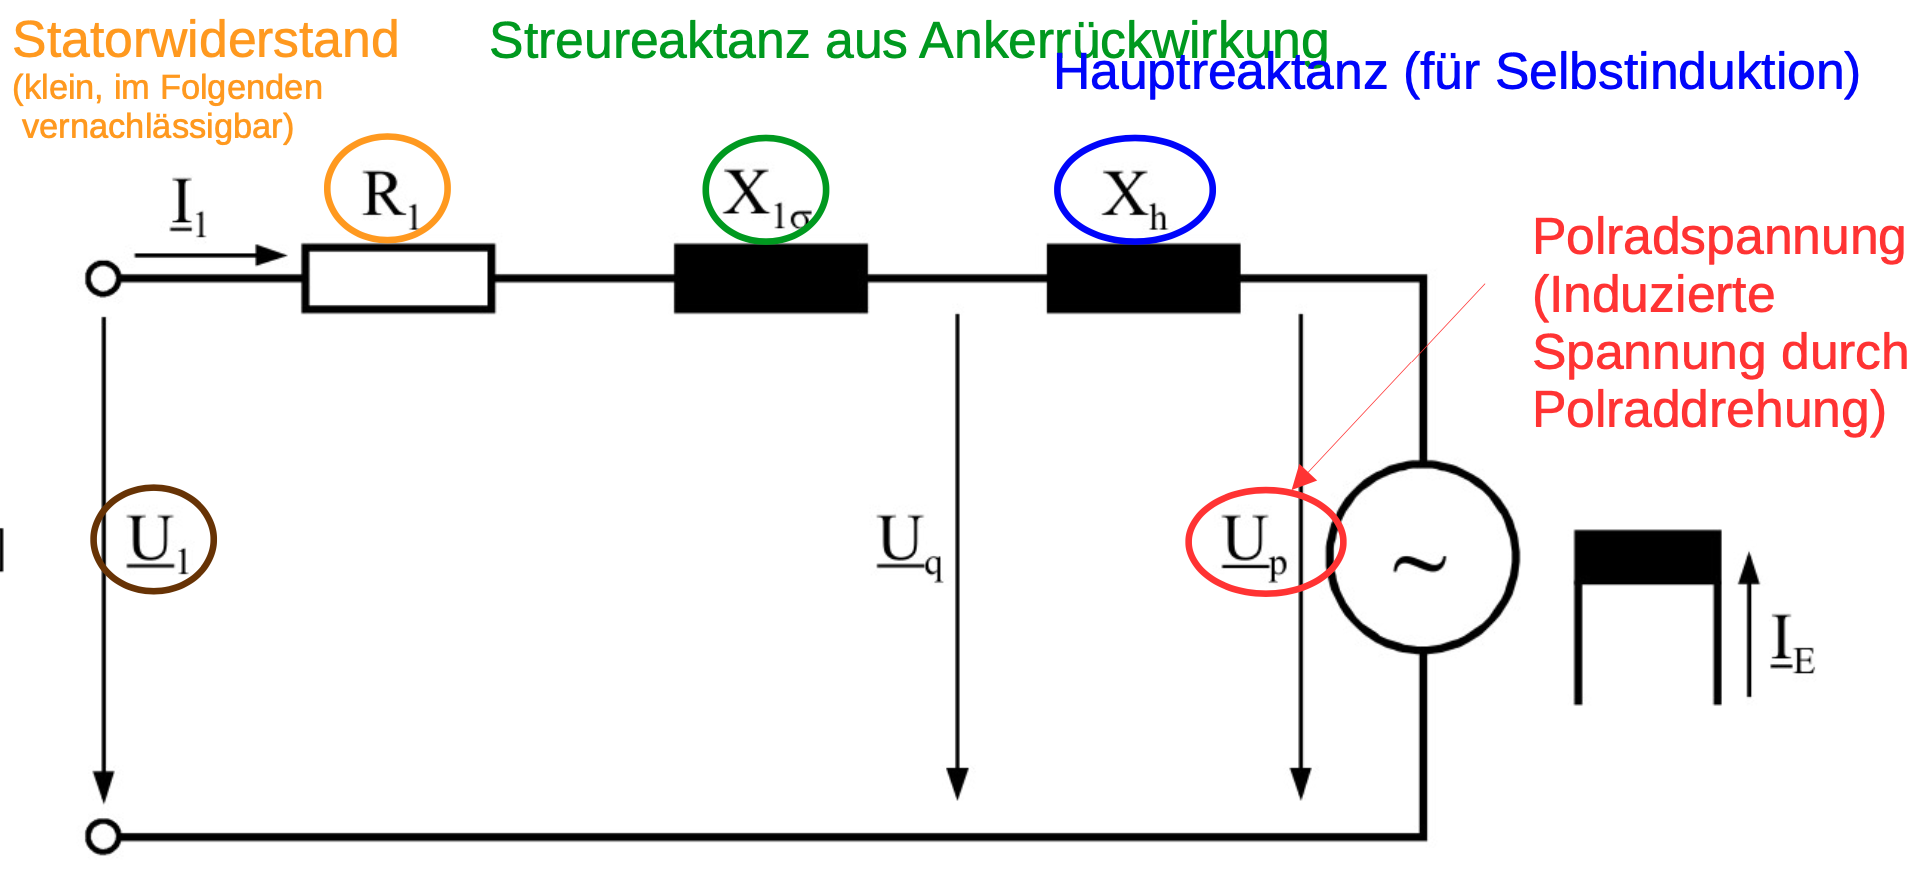
\includegraphics[width=0.85\linewidth]{images/ErsatzschaltbildSM.png}
\end{center}


\subsubsection{Beispiel Übererregter Generator}
\begin{minipage}[t]{0.49\columnwidth}
    Gegeben:
    \begin{itemize}
        \item Vekettete Spannung $U_n = 13\, \mathrm{kV}$
        \item Scheinleistung $S = 100~\mathrm{MVA}$ 
        \item $\cos{\varphi} = 0.87 $
        \item Synchrone Längsreaktanz $X_d =140\, \mathrm{\%}$ 
        \item Subtransiente Reaktanz  $X_d''=15\, \mathrm{\%}$
        \item Leerlauf Erregerstrom $I_{E0}$ 
        \item Drehzahl $n=600\, \mathrm{u/min}$
    \end{itemize}
\end{minipage}%
\hfill
\begin{minipage}[t]{0.49\columnwidth}
    Gesucht:
    \begin{itemize}
        \item Polradwinkel $\vartheta$
        \item Polradspannung $U_p$
        \item Erregerstrom $I_{En}$ für $X_h\approx const.$
        \item Polpaarzahl $p$
        \item Anfangskurzschlusswechselstrom $I_k''$
    \end{itemize}
\end{minipage}

\begin{align*}
    U_{1}       &= \frac{U_n}{\sqrt{3}} =\frac{13~\mathrm{kV}}{\sqrt{3}} = 7.5\, \mathrm{kV} \\
    X_n         &= X_d\cdot\frac{U_n^2}{S} = 1.4\cdot\frac{(23~\mathrm{kV})^2}{100~\mathrm{MVA}}=2.365\, \mathrm{\Omega}\\
    I_{1}       &= \frac{S}{3\cdot U_{1}} = \frac{100~MVA}{3 \cdot 7.5~kV} = 4.441~kA\\
    U_x         &= jX_n \cdot I_{1}= 2.37~\Omega \cdot 4.441~kA = 10.53~kV\\
                &\Rightarrow \text{$U_x$ in Zeigerdiag. mit Winkel $\varphi$ gegenüber $U_1$ eintragen, $U_p$ und $\vartheta$ auslesen}\\
                &\Rightarrow U_p = 15.5\, \mathrm{kV}, \vartheta = 35\, \mathrm{^\circ}\\
    I_{En}      &= I_{E0}\cdot\frac{U_p}{U_1}= 400\, \mathrm{A}\cdot\frac{15.5\, \mathrm{kV}}{7.5\, \mathrm{kV}} = 826\, \mathrm{A}\\
    p           &= \frac{60\cdot f}{n}= \frac{60\, \mathrm{min/s}\cdot 50\, \mathrm{Hz}}{600\, \mathrm{u/min}} = 5\\
    X_n''       &= X_d''\cdot\frac{U_n^2}{S}\\
    I_k''       &= \frac{U_1}{X_n''} \\
\end{align*}

\begin{center}
    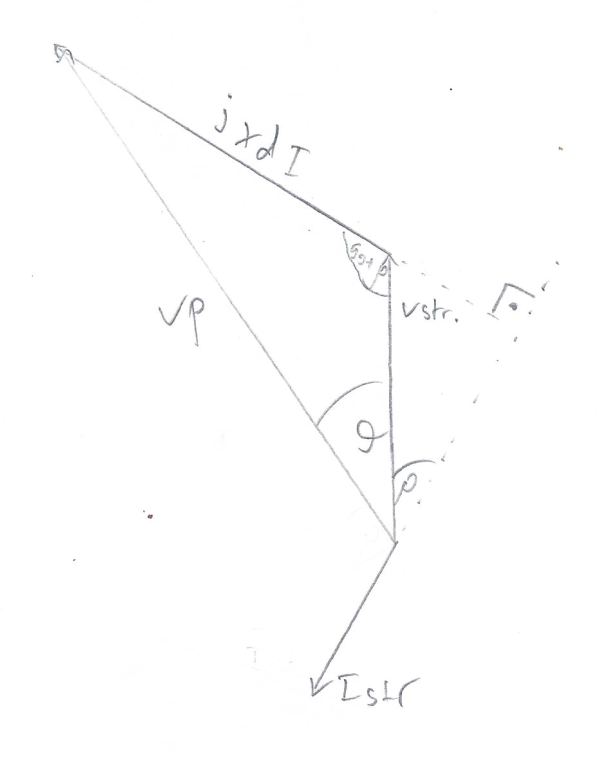
\includegraphics[width=0.75\columnwidth]{images/Maschinen2.png}
\end{center}

Verbesserung Wirkleistungsabgabe $\Rightarrow$ Turbinenregulierung

Verbesserung Blindleistungsabgabe $\Rightarrow$ SM-Erregung
 % done
        \section{Abschlussorgane bei Speicherkraftwerken}
\subsection{Schützen}
    \begin{tabular}{@{}ll}
        \textbf{Aufgabe:}                       & Binäre Regelung des Wasserdurchflusses („Auf und zu“)\\
        \textbf{Anwendung:}                     & Grundablass, Seeabschluss, Abschluss gegen das Unterwasser\\
        \textbf{\cgn{Vorteile:}}   & Einfacher Aufbau, sichere Absperrung\\
        \textbf{\crd{Nachteile:}}    & Keine Zwischenstellungen („halb offen“ nicht möglich)\\
        \textbf{Beispiel:}                      & Regulierschütz und Reserveschütz beim Grundablass\\
        \textbf{Sonstiges:}                     & Zwei Schützen pro Grundablass für Betrieb und Revision; \\
                                                & schnelle Schliess- und Öffnungszeiten sind entscheidend, \\
                                                & um Druckstösse zu vermeiden.\\
    \end{tabular}

\subsection{Klappen}
    \begin{tabular}{@{}ll}
        \textbf{Aufgabe:}                       & Wasserfluss absperren (Notverschluss, Wartung)\\
        \textbf{Anwendung:}                     & Saugrohrklappen beim Kraftwerk Mapragg\\
        \textbf{\cgn{Vorteile:}}   & Schnelles Schliessen, einfacher Aufbau\\
        \textbf{\crd{Nachteile:}}    & Keine Regelungsfunktion („halb offen“ nicht möglich)\\
        \textbf{Beispiel:}                      & Saugrohrklappen Mapragg\\
        \textbf{Sonstiges:}                     & Dienen als definitiver Abschluss bei Stillstand oder Wartung; \\
                                                & Schliess- und Öffnungszeiten dürfen nicht verändert werden, \\
                                                & um Druckstösse zu vermeiden.\\
    \end{tabular}

\subsection{Drosselklappen}
    \begin{tabular}{@{}ll}
        \textbf{Aufgabe:}                       & Regelbarer Durchfluss durch horizontales Verschieben \\
                                                & (Spalt lässt Wasser durch)\\
        \textbf{Anwendung:}                     & Einsatz bei variablen Durchflüssen\\
        \textbf{\cgn{Vorteile:}}   & Regelbarkeit des Durchflusses möglich\\
        \textbf{\crd{Nachteile:}}    & Höhere hydraulische Verluste\\
        \textbf{Beispiel:}                      & Horizontal verschiebbarer Rohrschieber\\
        \textbf{Sonstiges:}                     & Wird nur selten bei Speicher- oder Laufwasserkraftwerken eingesetzt, \\
                                                & da dort meist binäre Regelung bevorzugt wird.\\
    \end{tabular}

\subsection{Kugelschieber}
    \begin{tabular}{@{}ll}
        \textbf{Aufbau:}                        & Drehbare Kugel mit Loch\\
        \textbf{Aufgabe:}                       & Absperren des Wasserflusses mit nahezu verlustfreiem Durchfluss im offenen Zustand\\
        \textbf{Anwendung:}                     & Definitiver Abschluss (Betriebsring und Reservering)\\
        \textbf{\cgn{Vorteile:}}   & Im offenen Zustand nahezu verlustfrei\\
        \textbf{\crd{Nachteile:}}    & Wartung und Betrieb der Dichtung (Betriebsring) aufwändig\\
        \textbf{Beispiel:}                      & Kugelschieber in Wasserkraftwerken mit Betriebsring und Reservering\\
        \textbf{Sonstiges:}                     & Betriebsring sorgt für Abdichtung zwischen Gehäuse und Kugel, \\
                                                & Reservering wird nur bei Revision geschlossen und \\
                                                & gegen Wiederöffnen gesichert.\\
    \end{tabular}

\subsection{Ring- und Eckringschieber}
\begin{tabular}{@{}ll}
    \textbf{Aufgabe:}                       & Steuerung des Wasserflusses innerhalb oder ausserhalb des Rohres\\
    \textbf{Anwendung:}                     & Ringschieber: innerh. des Rohres; Eckringschieber: ausserh. des Rohres\\
    \textbf{\cgn{Vorteile:}}   & Flexibler Einbau, verschiedene Steuerungsmöglichkeiten\\
    \textbf{\crd{Nachteile:}}    & Erhöhter Konstruktions- und Wartungsaufwand\\
    \textbf{Beispiel:}                      & Ringschieber und Eckringschieber bei variablen Wasserführungen\\
    \textbf{Sonstiges:}                     & Ermöglichen Zwischenstellungen (feine Regelung), \\
                                            & können jedoch zu höheren hydraulischen Verlusten führen.\\
\end{tabular} % done
        \input{sections/13_Stauanlagen_Laufwasserkraftwerke.tex} % done
        \section{Wasserkraftwerk-Typen}
\subsection{Klassifizierung}
    \vspace{-4mm}
    \def\columnseprulecolor{\color{white}}
    \begin{multicols}{2}
        \begin{itemize}
            \item Laufwasserkraftwerke
            \item Mitteldruckanlagen
            \item Hochdruck- (Speicher-) Anlagen
            \item Pumpspeicherkraftwerke
            \item Gezeitenkraftwerke
            \item Wellenkraftwerke
            \item Wasserwirbelkraftwerke
        \end{itemize}
    \end{multicols}
    \def\columnseprulecolor{\color{black}}

\subsection{Einteilung nach technischen Aspekten}
\vspace{-4mm}
    \def\columnseprulecolor{\color{white}}
    \begin{multicols}{2}
\begin{itemize}
    \item \textbf{Laufwasserkraftwerke}
    \begin{itemize}
        \item Flusskraftwerke
        \begin{itemize}
            \item Blockbauweise
            \item Buchtenkraftwerke
            \item Zwillingsbauweise 
            \item[] (beidseitige Anordnung)
            \item Ausleitkraftwerke
            \item \dots
        \end{itemize}
        \item Ausleitungskraftwerke
    \end{itemize}
    \item \textbf{Speicherkraftwerke} 
    \item[] mit natürlichem Zufluss
    \item \textbf{Pumpspeicherkraftwerke} 
    \item[] (Speicherkraftwerke mit oder ohne natürlichem Zufluss)
    \item Gezeitenkraftwerke
    \item Wellenkraftwerke
\end{itemize}
\end{multicols}
\def\columnseprulecolor{\color{black}}

\subsection{Einteilung nach energiewirtschaftlichen Aspekten}
\begin{itemize}
    \item Grundlastkraftwerke (häufig verwendet, Laufwasser, Speicher mit vielen Volllaststunden)
    \item Mittellastkraftwerke
    \item Spitzenlastkraftwerke (Speicher mit wenig Volllaststunden)
\end{itemize}

\subsection{Einteilung nach Betriebsart}
\begin{itemize}
    \item Verbundbetrieb (im Normalbetrieb alle Kraftwerke in der Schweiz)
    \item Inselbetrieb (Unabhängig vom Netz)
\end{itemize}

\subsection{Einteilung nach der installierten Leistung}
\begin{itemize}
    \item Kleinwasserkraftwerke (in der Regel kleiner 10 MW)
    \item Grosswasserkraftwerke (P > 10 MW)
\end{itemize}

\subsection{Einteilung nach wasserwirtschaftlichen Aspekten}
\begin{itemize}
    \item Wasserkraftwerke, die ausschliesslich elektrische Energie produzieren
    \item Wasserkraftanlagen für mehrere wasserwirtschaftliche Zielsetzungen (Mehrzweckanlagen, z.\,B. Trinkwasser)
\end{itemize}

\subsection{Wasserturbinen und Pumpen}
\begin{itemize}
    \item \textbf{Aktionsturbinen:} Arbeit aus kinetischer Energie-Differenz
    \begin{itemize}
        \item \textbf{Peltonturbinen}
    \end{itemize}
    \item \textbf{Reaktionsturbinen:} Arbeit aus Druckdifferenz vor und nach Turbine
        \begin{itemize}
            \item \textbf{Francisturbinen} (spiralförmig)
            \item \textbf{Kaplanturbinen} (propellerförmig)
            \item Rohrturbinen
            \item Kreiselpumpen als Turbinen
        \end{itemize}
\end{itemize}

\subsection{Laufwasserkraftwerke (LWK)}    
    \begin{minipage}[c]{0.7\columnwidth}
        \begin{center}
            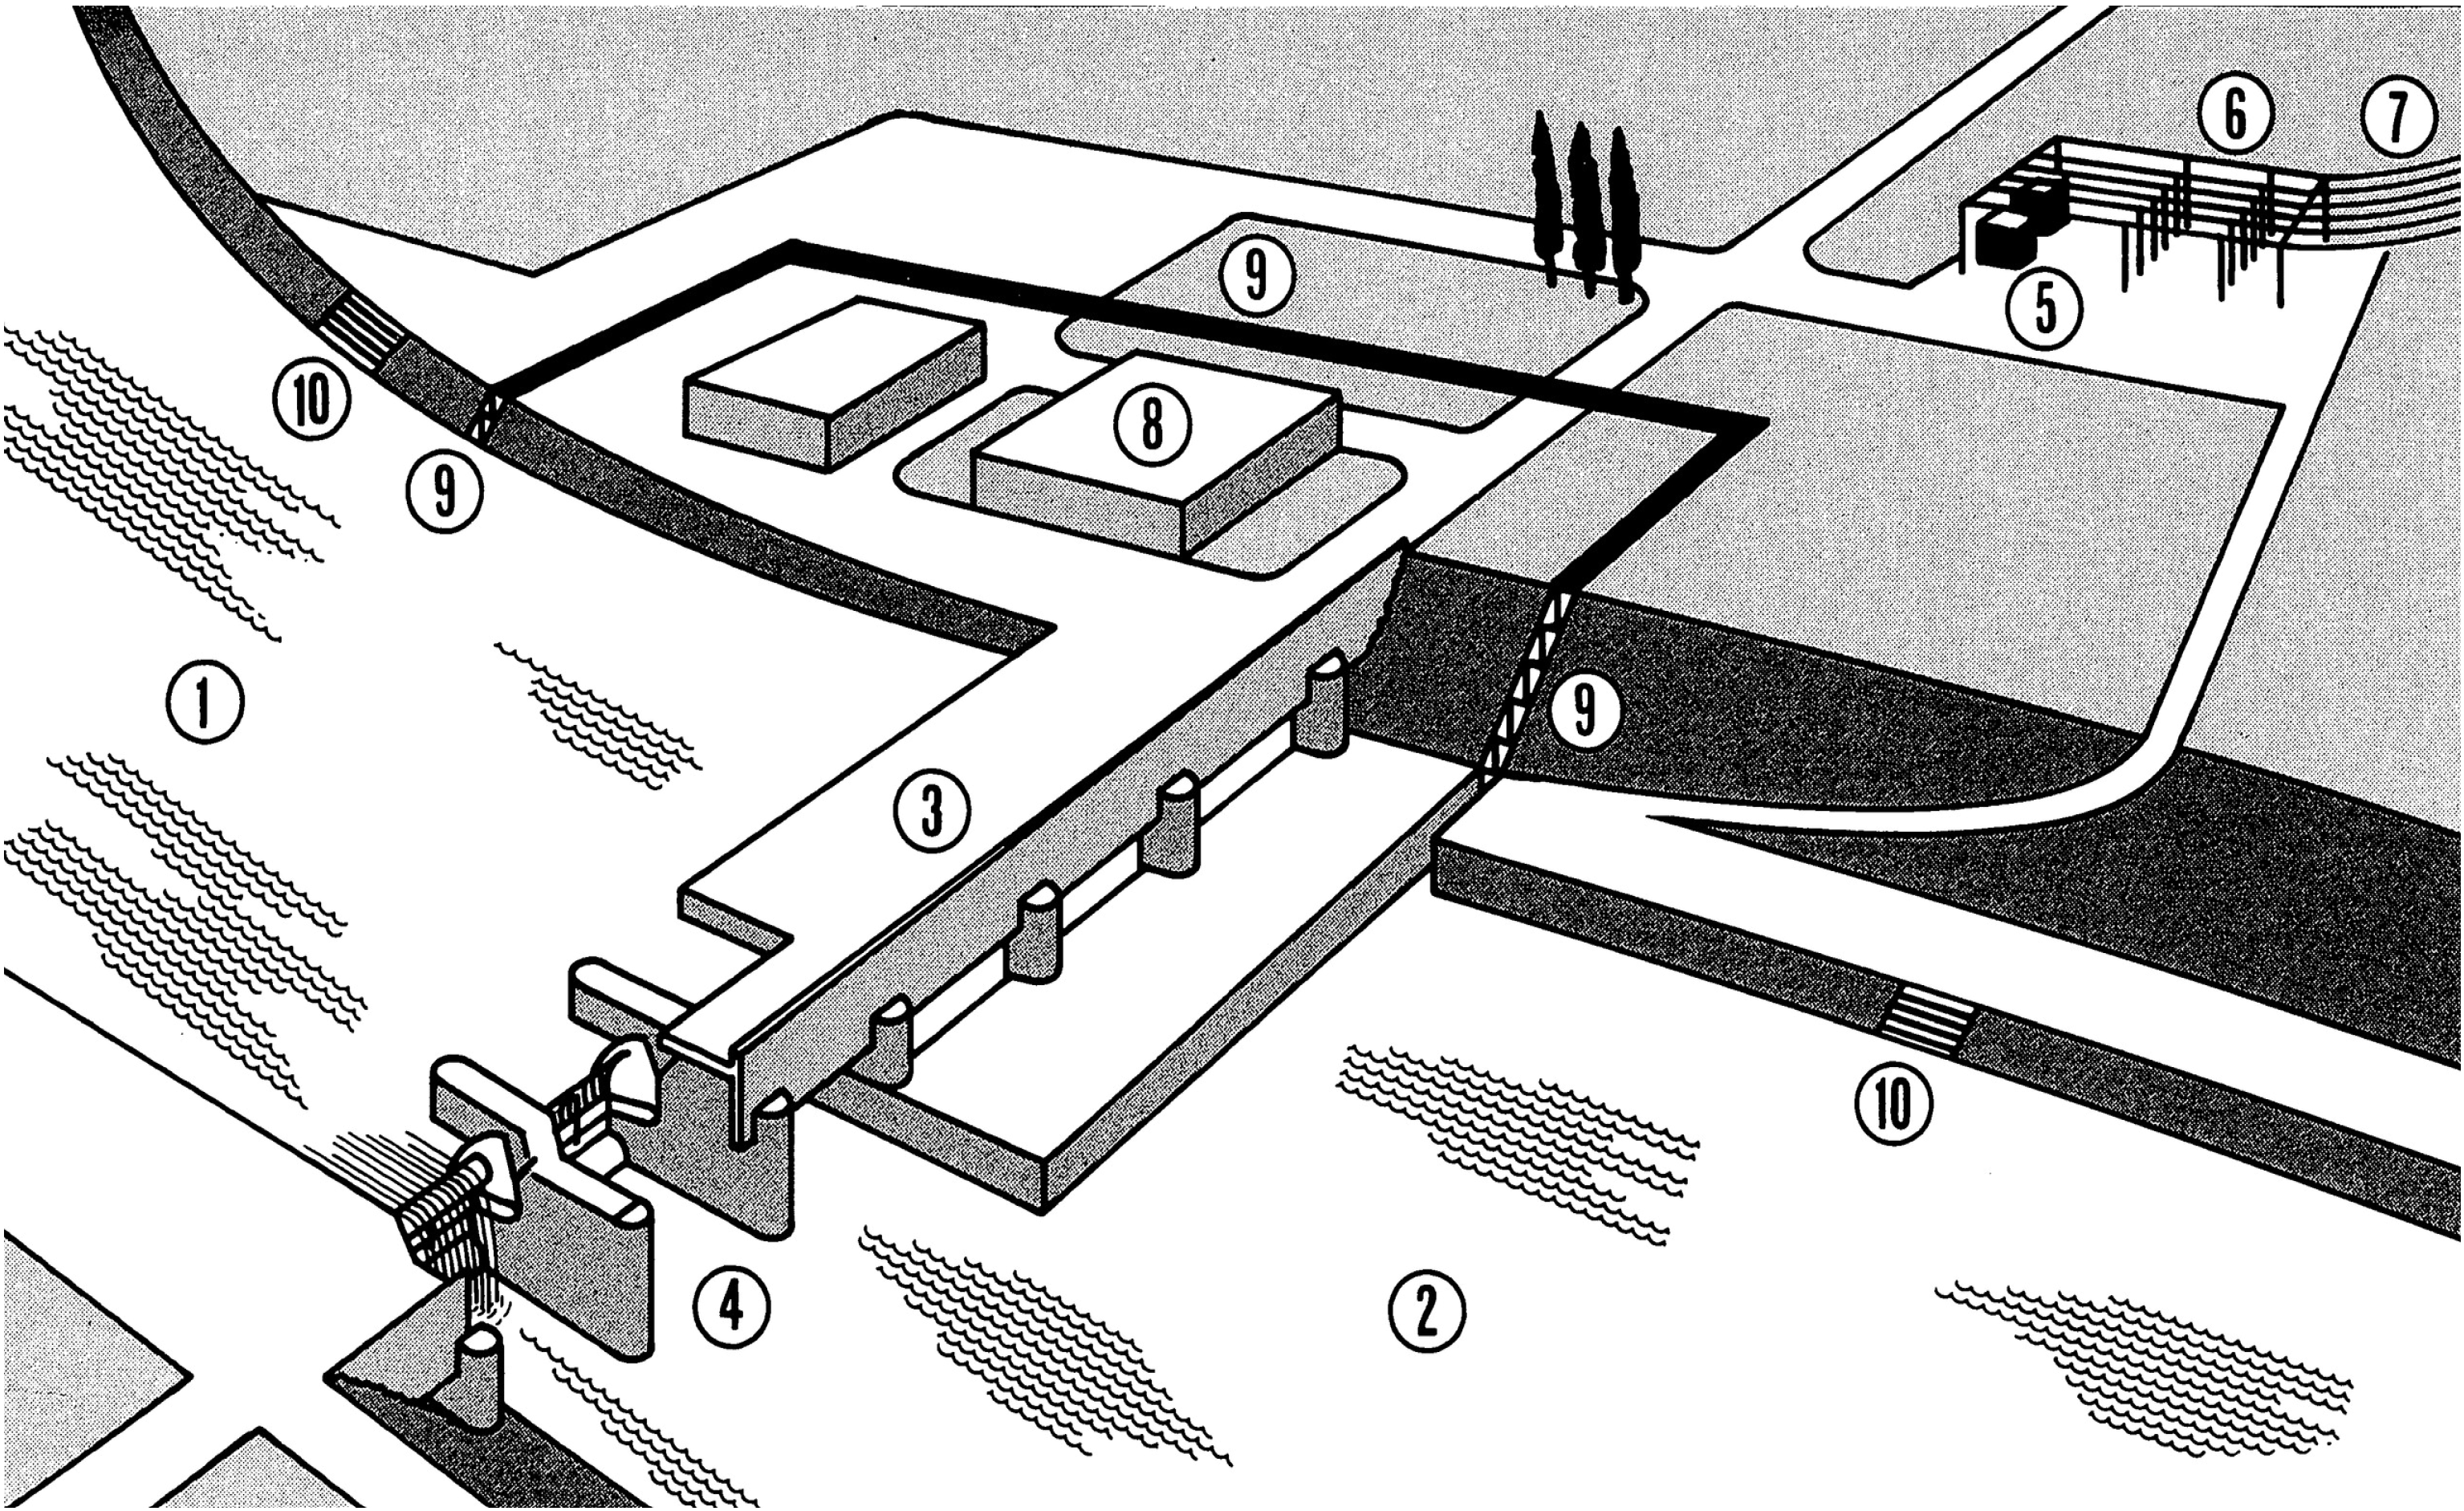
\includegraphics[width=0.95\columnwidth]{images/Laufwasserkraftwerke.png}
        \end{center}
    \end{minipage}
    \hfill
    \begin{minipage}[c]{0.29\columnwidth}
        \begin{enumerate}
            \item Oberwasser 
            \item Unterwasser 
            \item Maschinenhaus
            \item Stauwehr
            \item Transformatoren
            \item Schaltanlage
            \item Leitungen
            \item Betriebsgebäude
            \item Fischtreppe
            \item Einrichtung für den Schiffstransport
        \end{enumerate}
    \end{minipage}

\subsection{LWK mit Kaplanturbinen (vertikal)}
    \begin{center}
        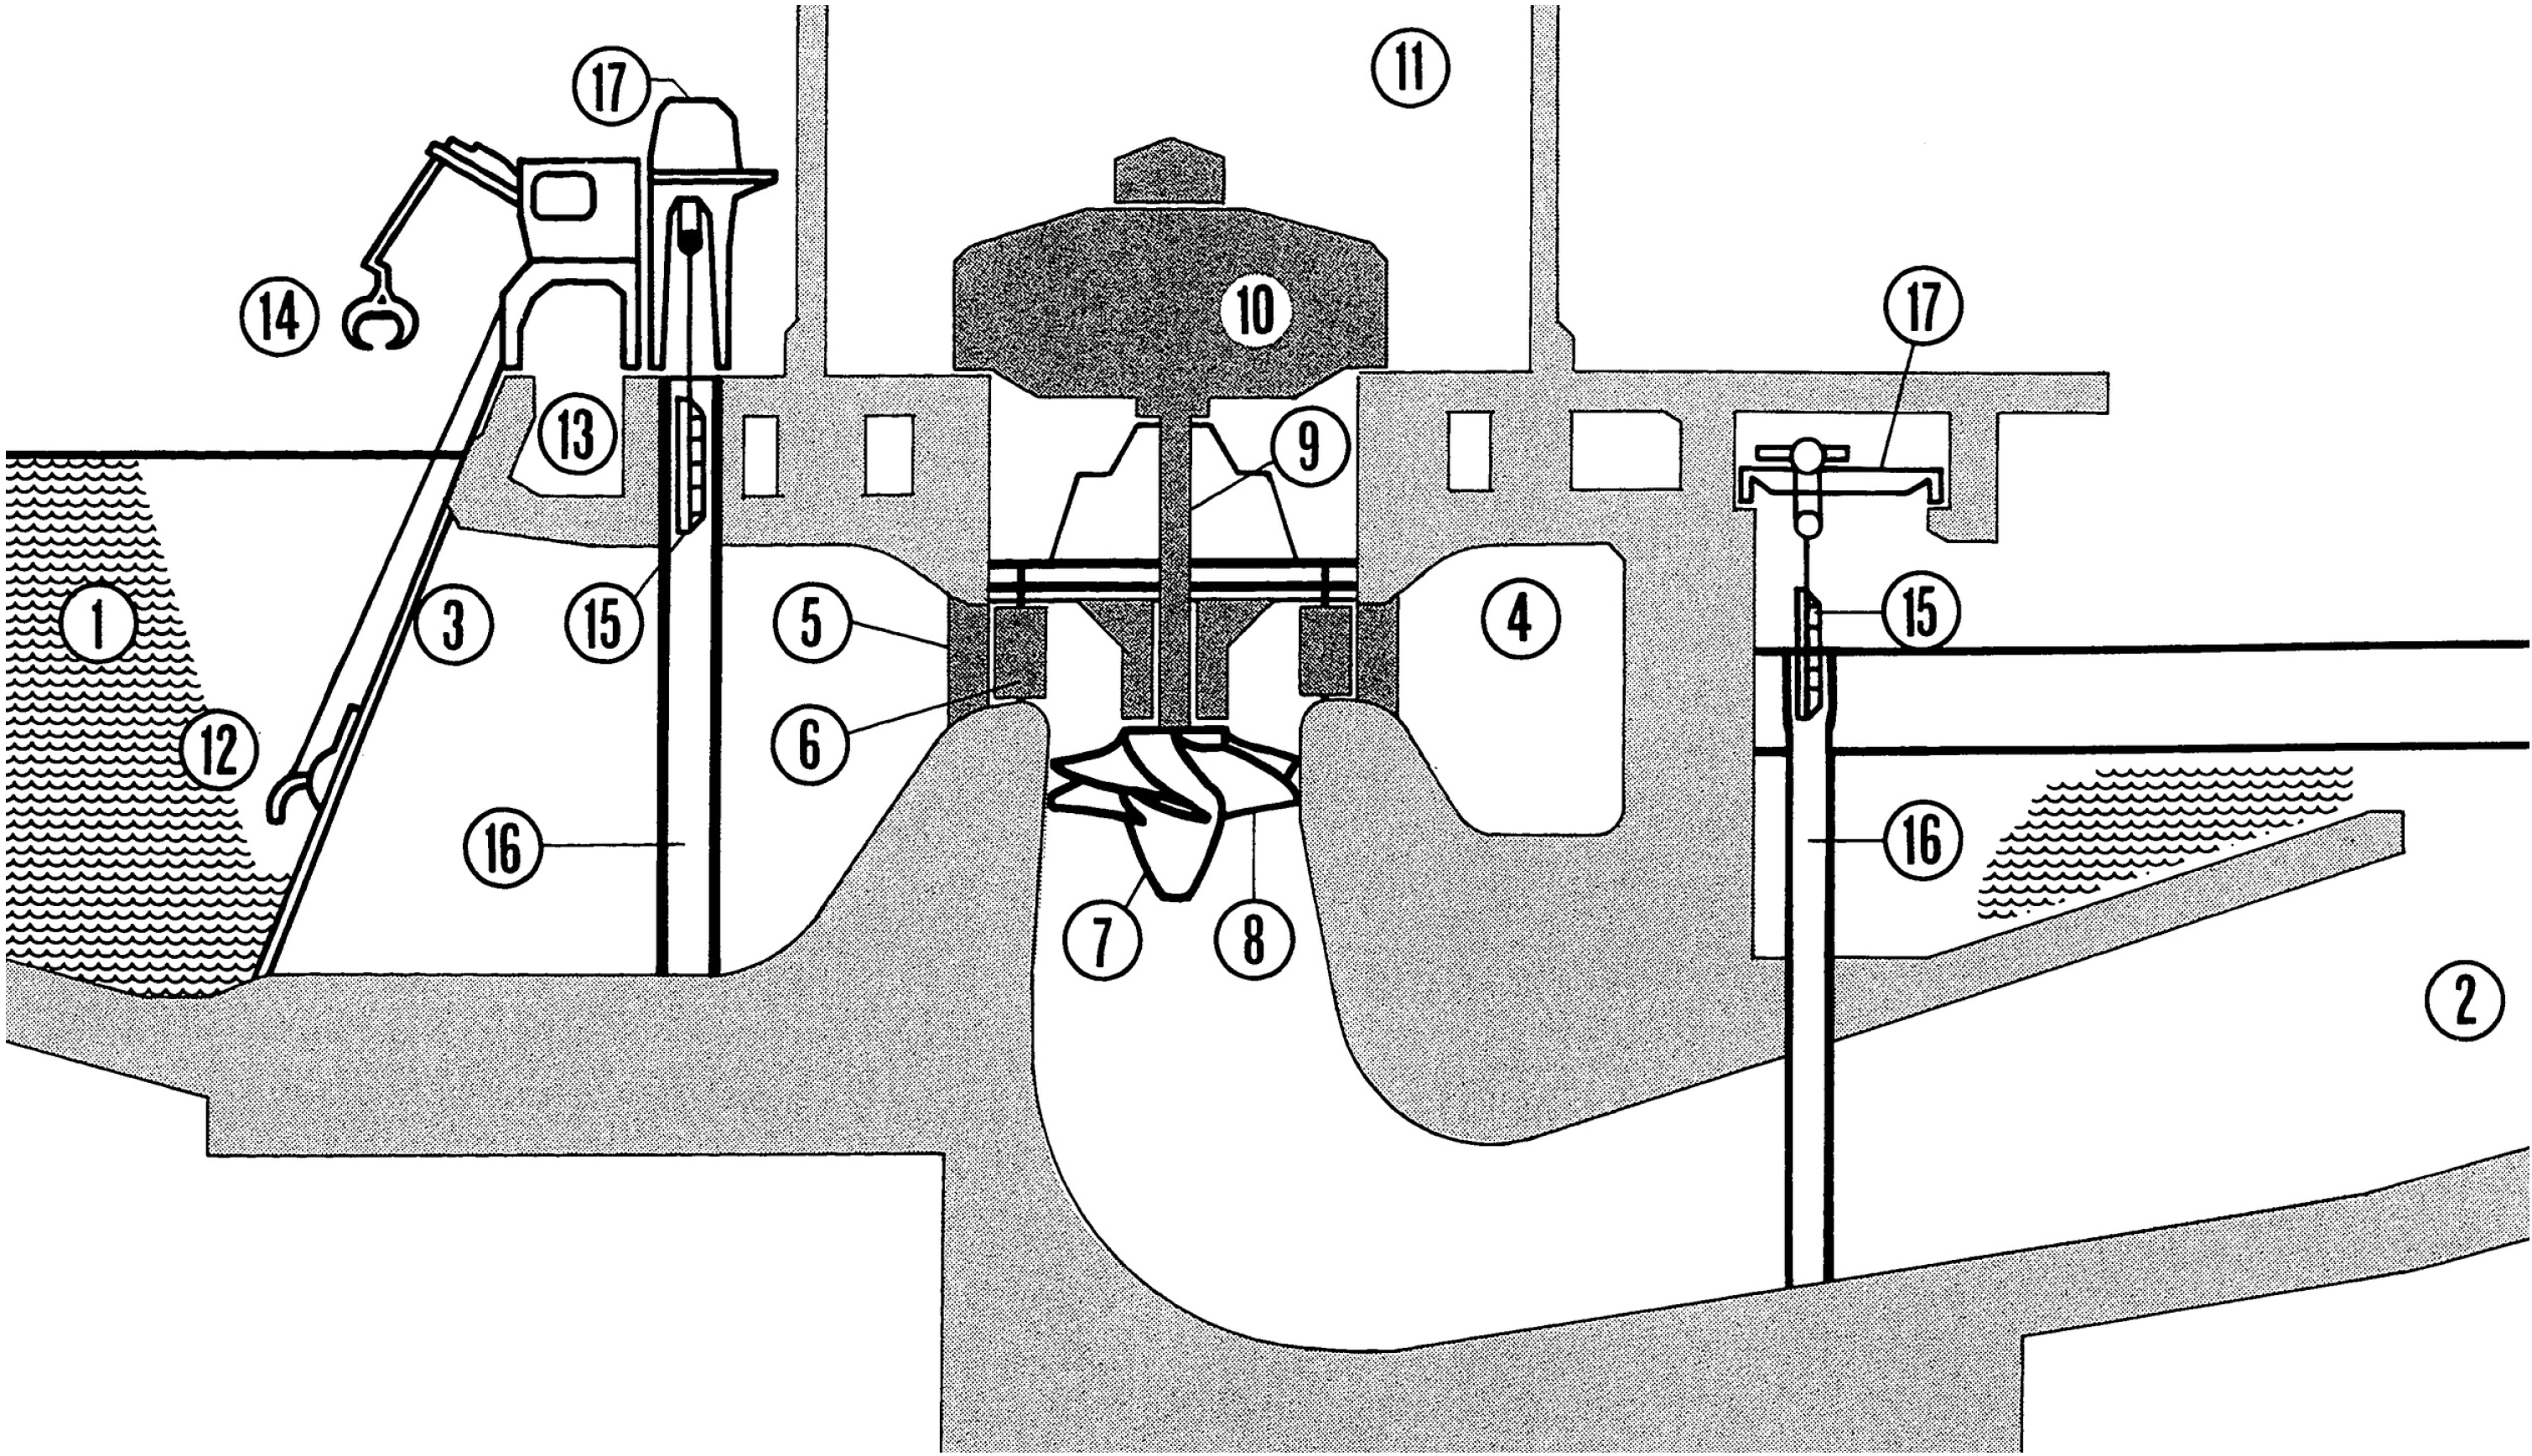
\includegraphics[width=0.75\columnwidth]{images/Laufwasserkraftwerke_Kaplanturbine_Vertikal.png}
    \end{center}

    \vspace{-4mm}
    \def\columnseprulecolor{\color{white}}
    \begin{multicols}{3}
        \begin{enumerate}
            \item Oberwasser
            \item Unterwasser
            \item Rechen
            \item Spirale
            \item Stützschaufeln
            \item Leitschaufeln
            \item Laufrad
            \item Laufradschaufeln
            \item Saugrohr
            \item Generator
            \item Maschinenhaus
            \item Rechenreinigungsmaschine
            \item Geschwemmselrinne
            \item Zangengreifer
            \item Dammbalken
            \item Nuten für Dammbalken
            \item Dammbalkenkran
        \end{enumerate}
    \end{multicols}
    \def\columnseprulecolor{\color{black}}

\subsection{LWK mit Rohrturbinen (horizontal, bis 25m Fallhöhe)}
    \begin{center}
        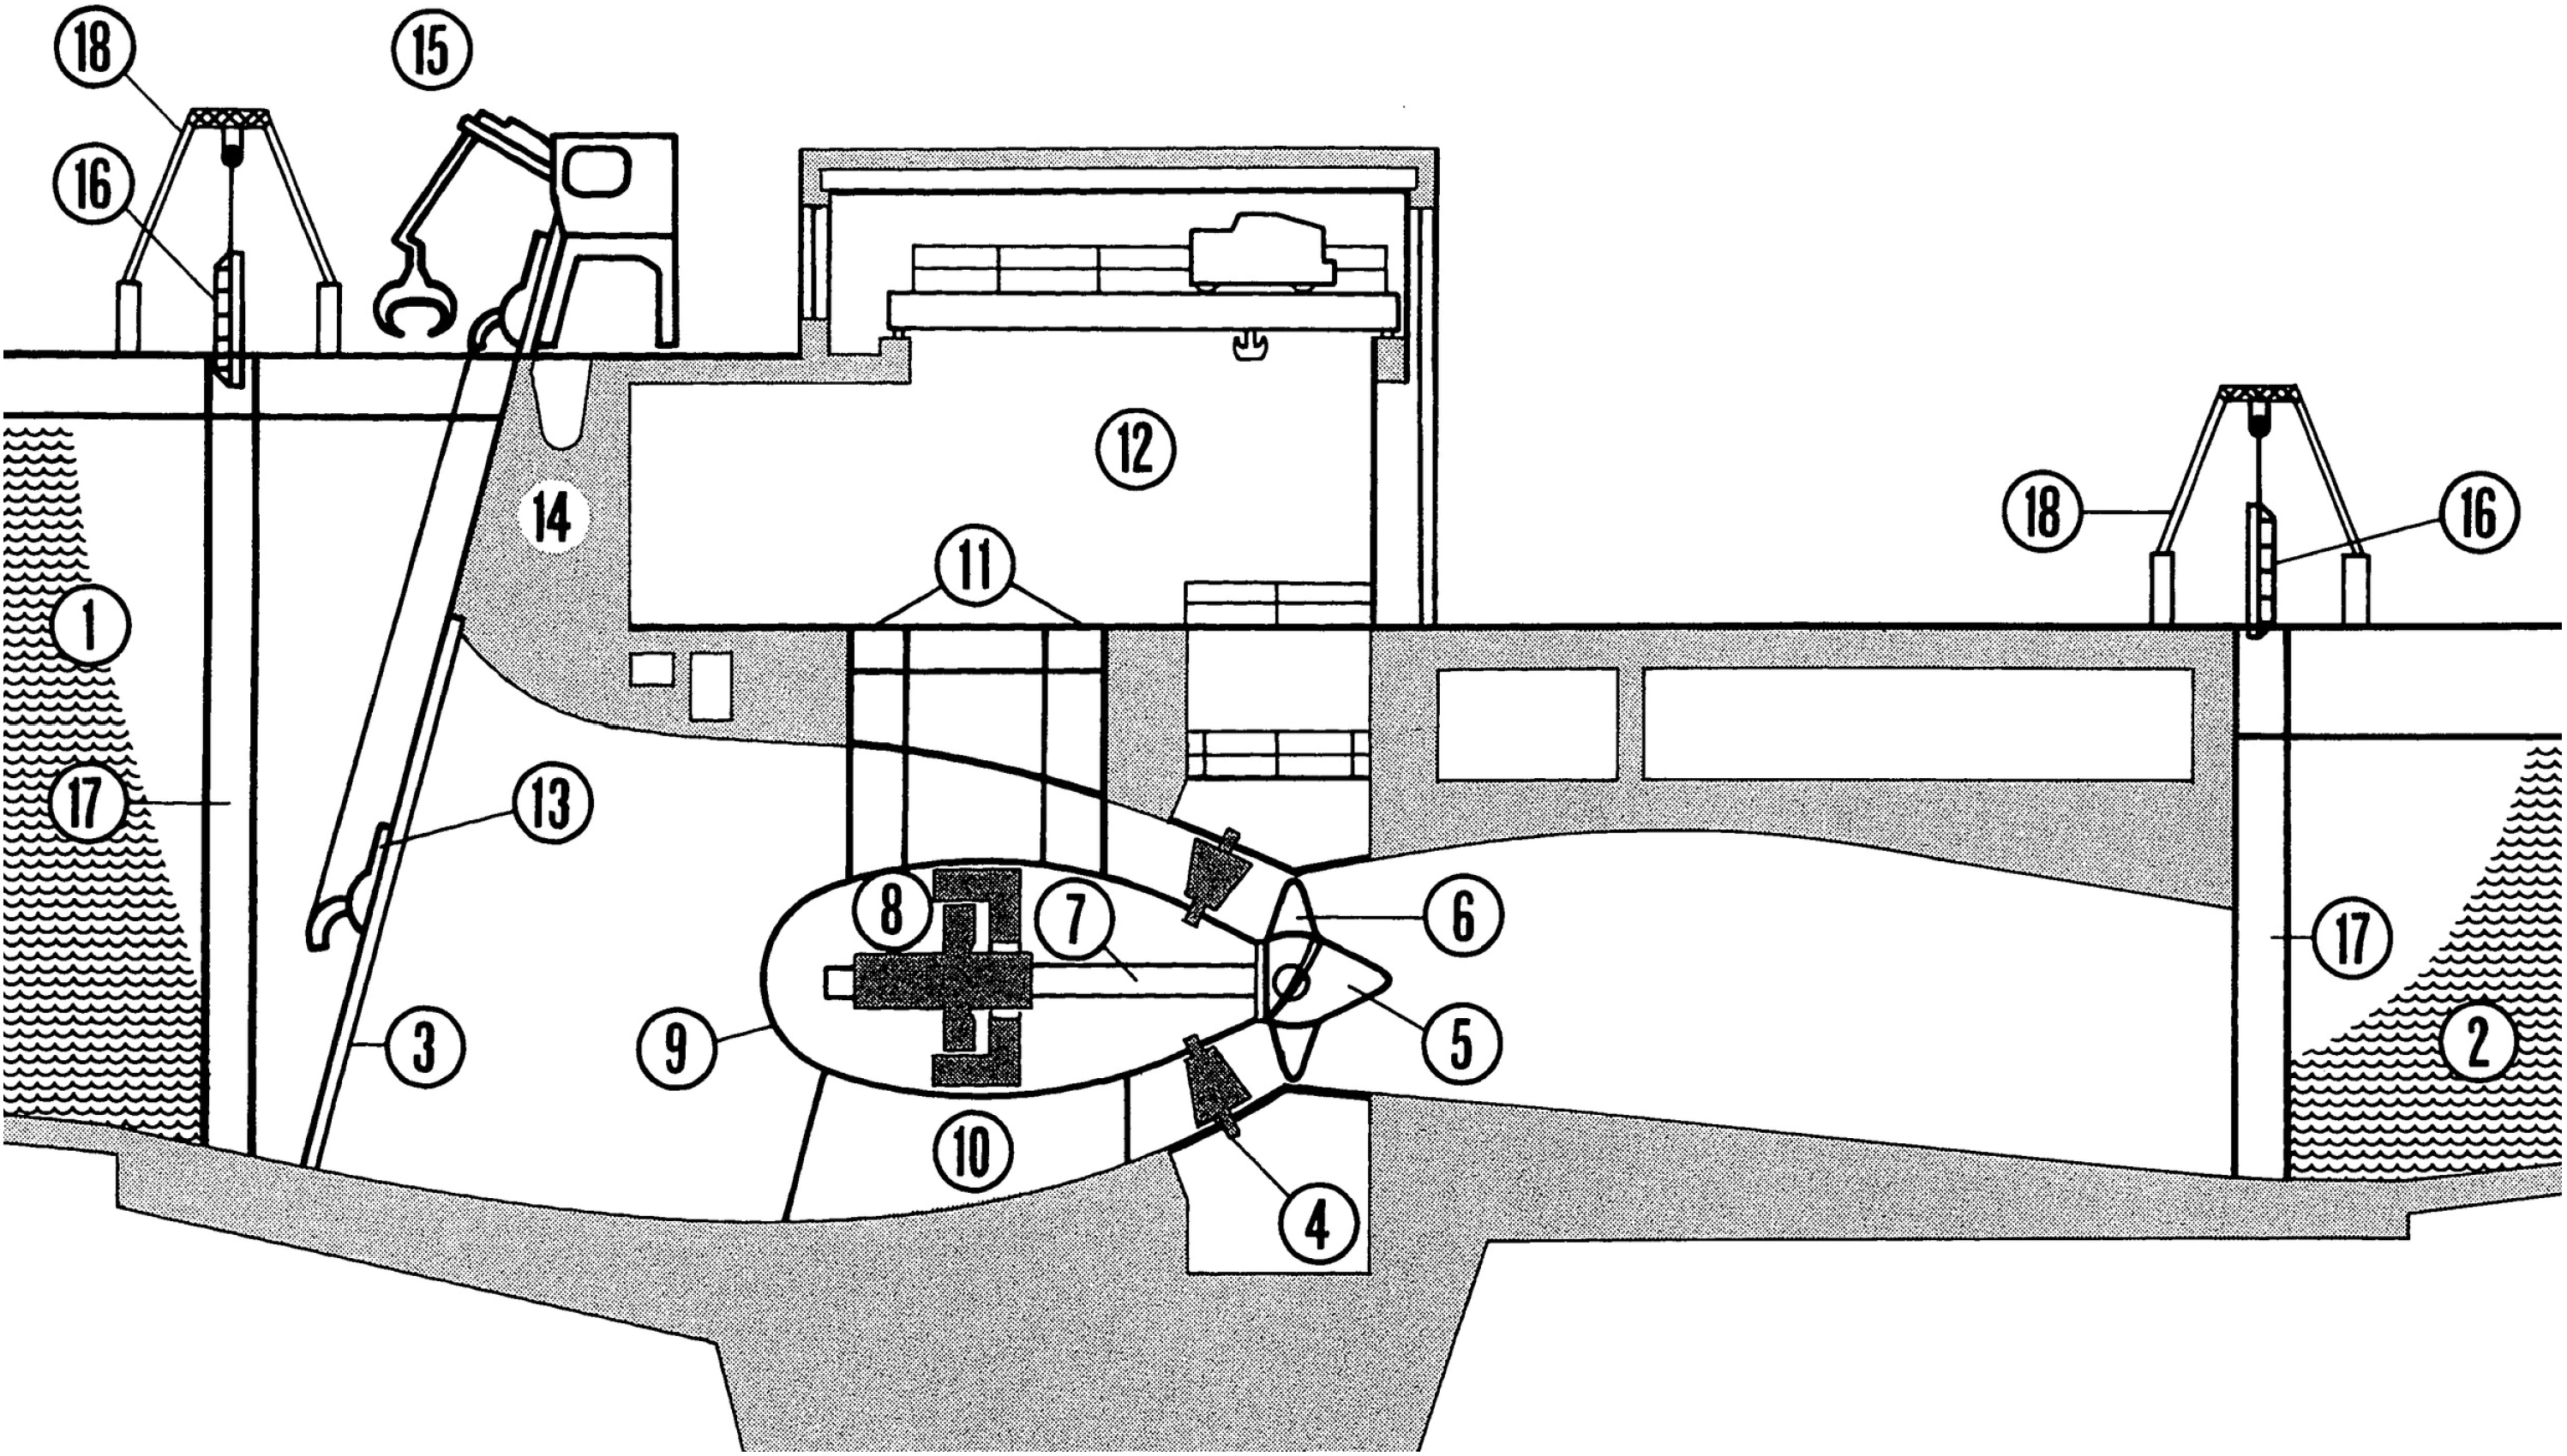
\includegraphics[width=0.9\columnwidth]{images/Laufwasserkraftwerke_Kaplanturbine_Horizontal.png}
    \end{center}

    \vspace{-4mm}
    \def\columnseprulecolor{\color{white}}
    \begin{multicols}{3}
        \begin{enumerate}
            \item Oberwasser
            \item Unterwasser
            \item Rechen
            \item Leitschaufeln
            \item Laufrad
            \item Laufradschaufeln
            \item Turbinenwelle
            \item Generator
            \item Gehäuse
            \item Sockel
            \item Einstiegsschächte
            \item Maschinenhalle
            \item Rechenreinigungsmasch.
            \item Geschwemmselrinne
            \item Zangengreifer
            \item Dammbalken
            \item Nuten für Dammbalken
            \item Dammbalkenkran
        \end{enumerate}
    \end{multicols}
    \def\columnseprulecolor{\color{black}}

\subsection{Wasserwirbelkraftwerk}
    \begin{minipage}[c]{0.58\columnwidth}
        \begin{itemize}
        \item Für Kleinwasserkraft
        \item Geringe Fallhöhen und Durchfluss möglich:\\
        $h \geqq 0.5\text{m}$ und $Q \geqq 0.5 \frac{\text{m}^3}{\text{s}}$
        \item Geringerer Wirkungsgrad
        \item Besser Fischgängig
    \end{itemize}
    \end{minipage}
    \hfill
    \begin{minipage}[c]{0.38\columnwidth}
        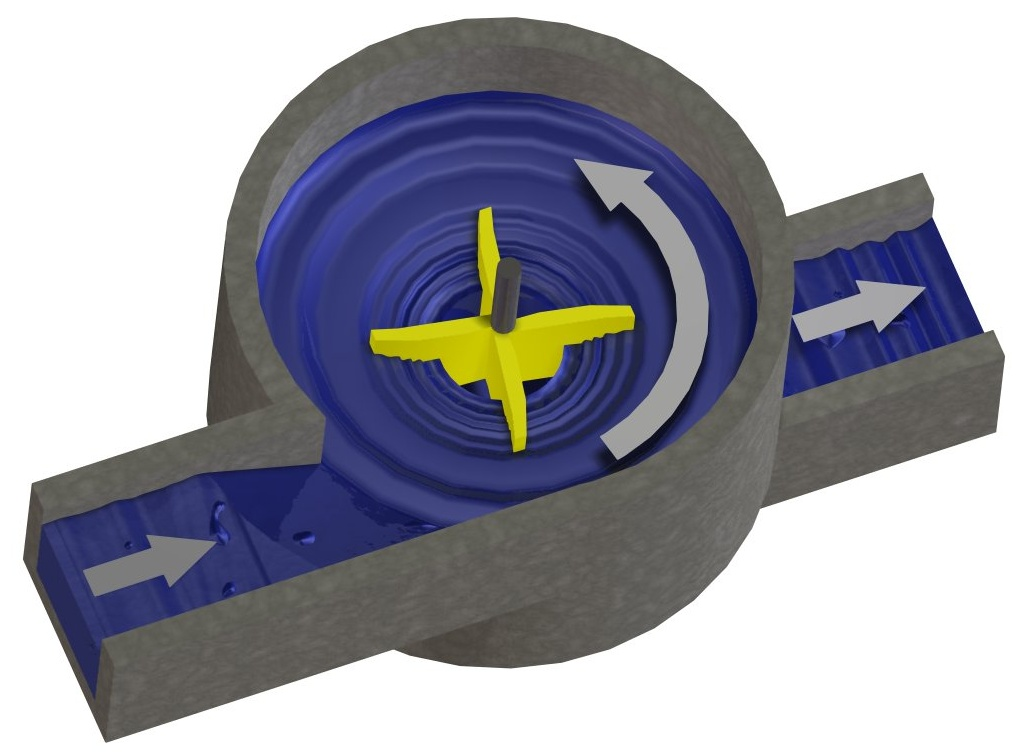
\includegraphics[width=0.65\columnwidth]{images/Wasserwirbelkraftwerk.jpg}
    \end{minipage}

\subsection{LWK mit Strafloturbinen}
    \begin{minipage}[c]{0.7\columnwidth}
        \begin{center}
            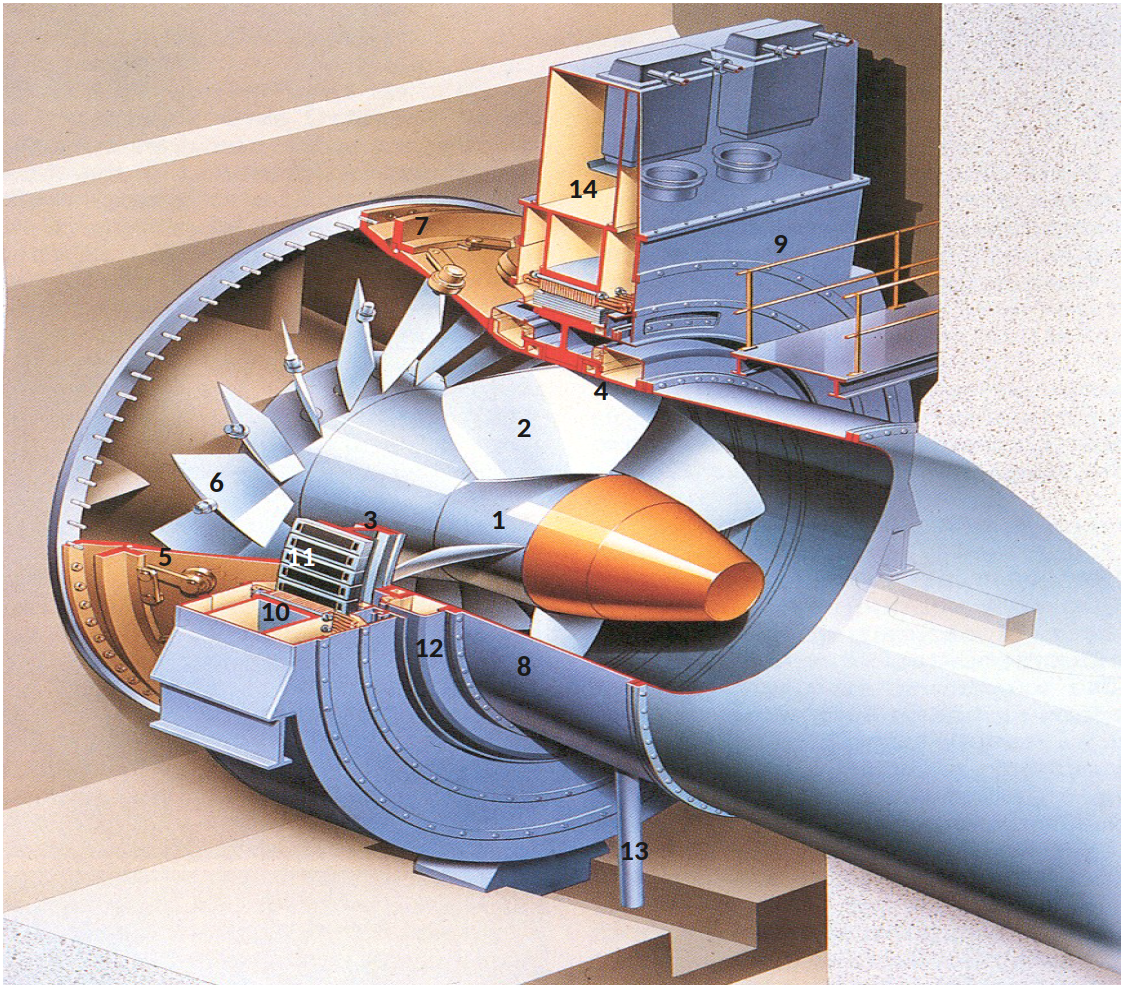
\includegraphics[width=0.95\columnwidth]{images/Laufwasserkraftwerke_mit_Strafloturbinen.png}
        \end{center}
    \end{minipage}
    \hfill
    \begin{minipage}[c]{0.29\columnwidth}
        \begin{enumerate}
            \item Laufradnabe
            \item Propellerblatt
            \item Rotorring
            \item Entlastungsring
            \item Turbinengehäuse
            \item Leitschaufel
            \item Leitradverstellring
            \item Rohrleitung
            \item Generator
            \item Stator
            \item Rotor
            \item Ringdichtungs-Leck"-wasser-Kollektor
            \item Leckwasserableitung
            \item Kühler
        \end{enumerate}
    \end{minipage}

    Weiterentwicklung der Rohrturbine, Rotor Turbine und Generator bilden Einheit

\subsection{Mitteldruckanlagen}
    bis circa 50m Fallhöhe (<= 5 bar Druck)

\subsection{Pumpspeicherkraftwerke (PSW)}
    \begin{minipage}[c]{0.7\columnwidth}
        \begin{center}
            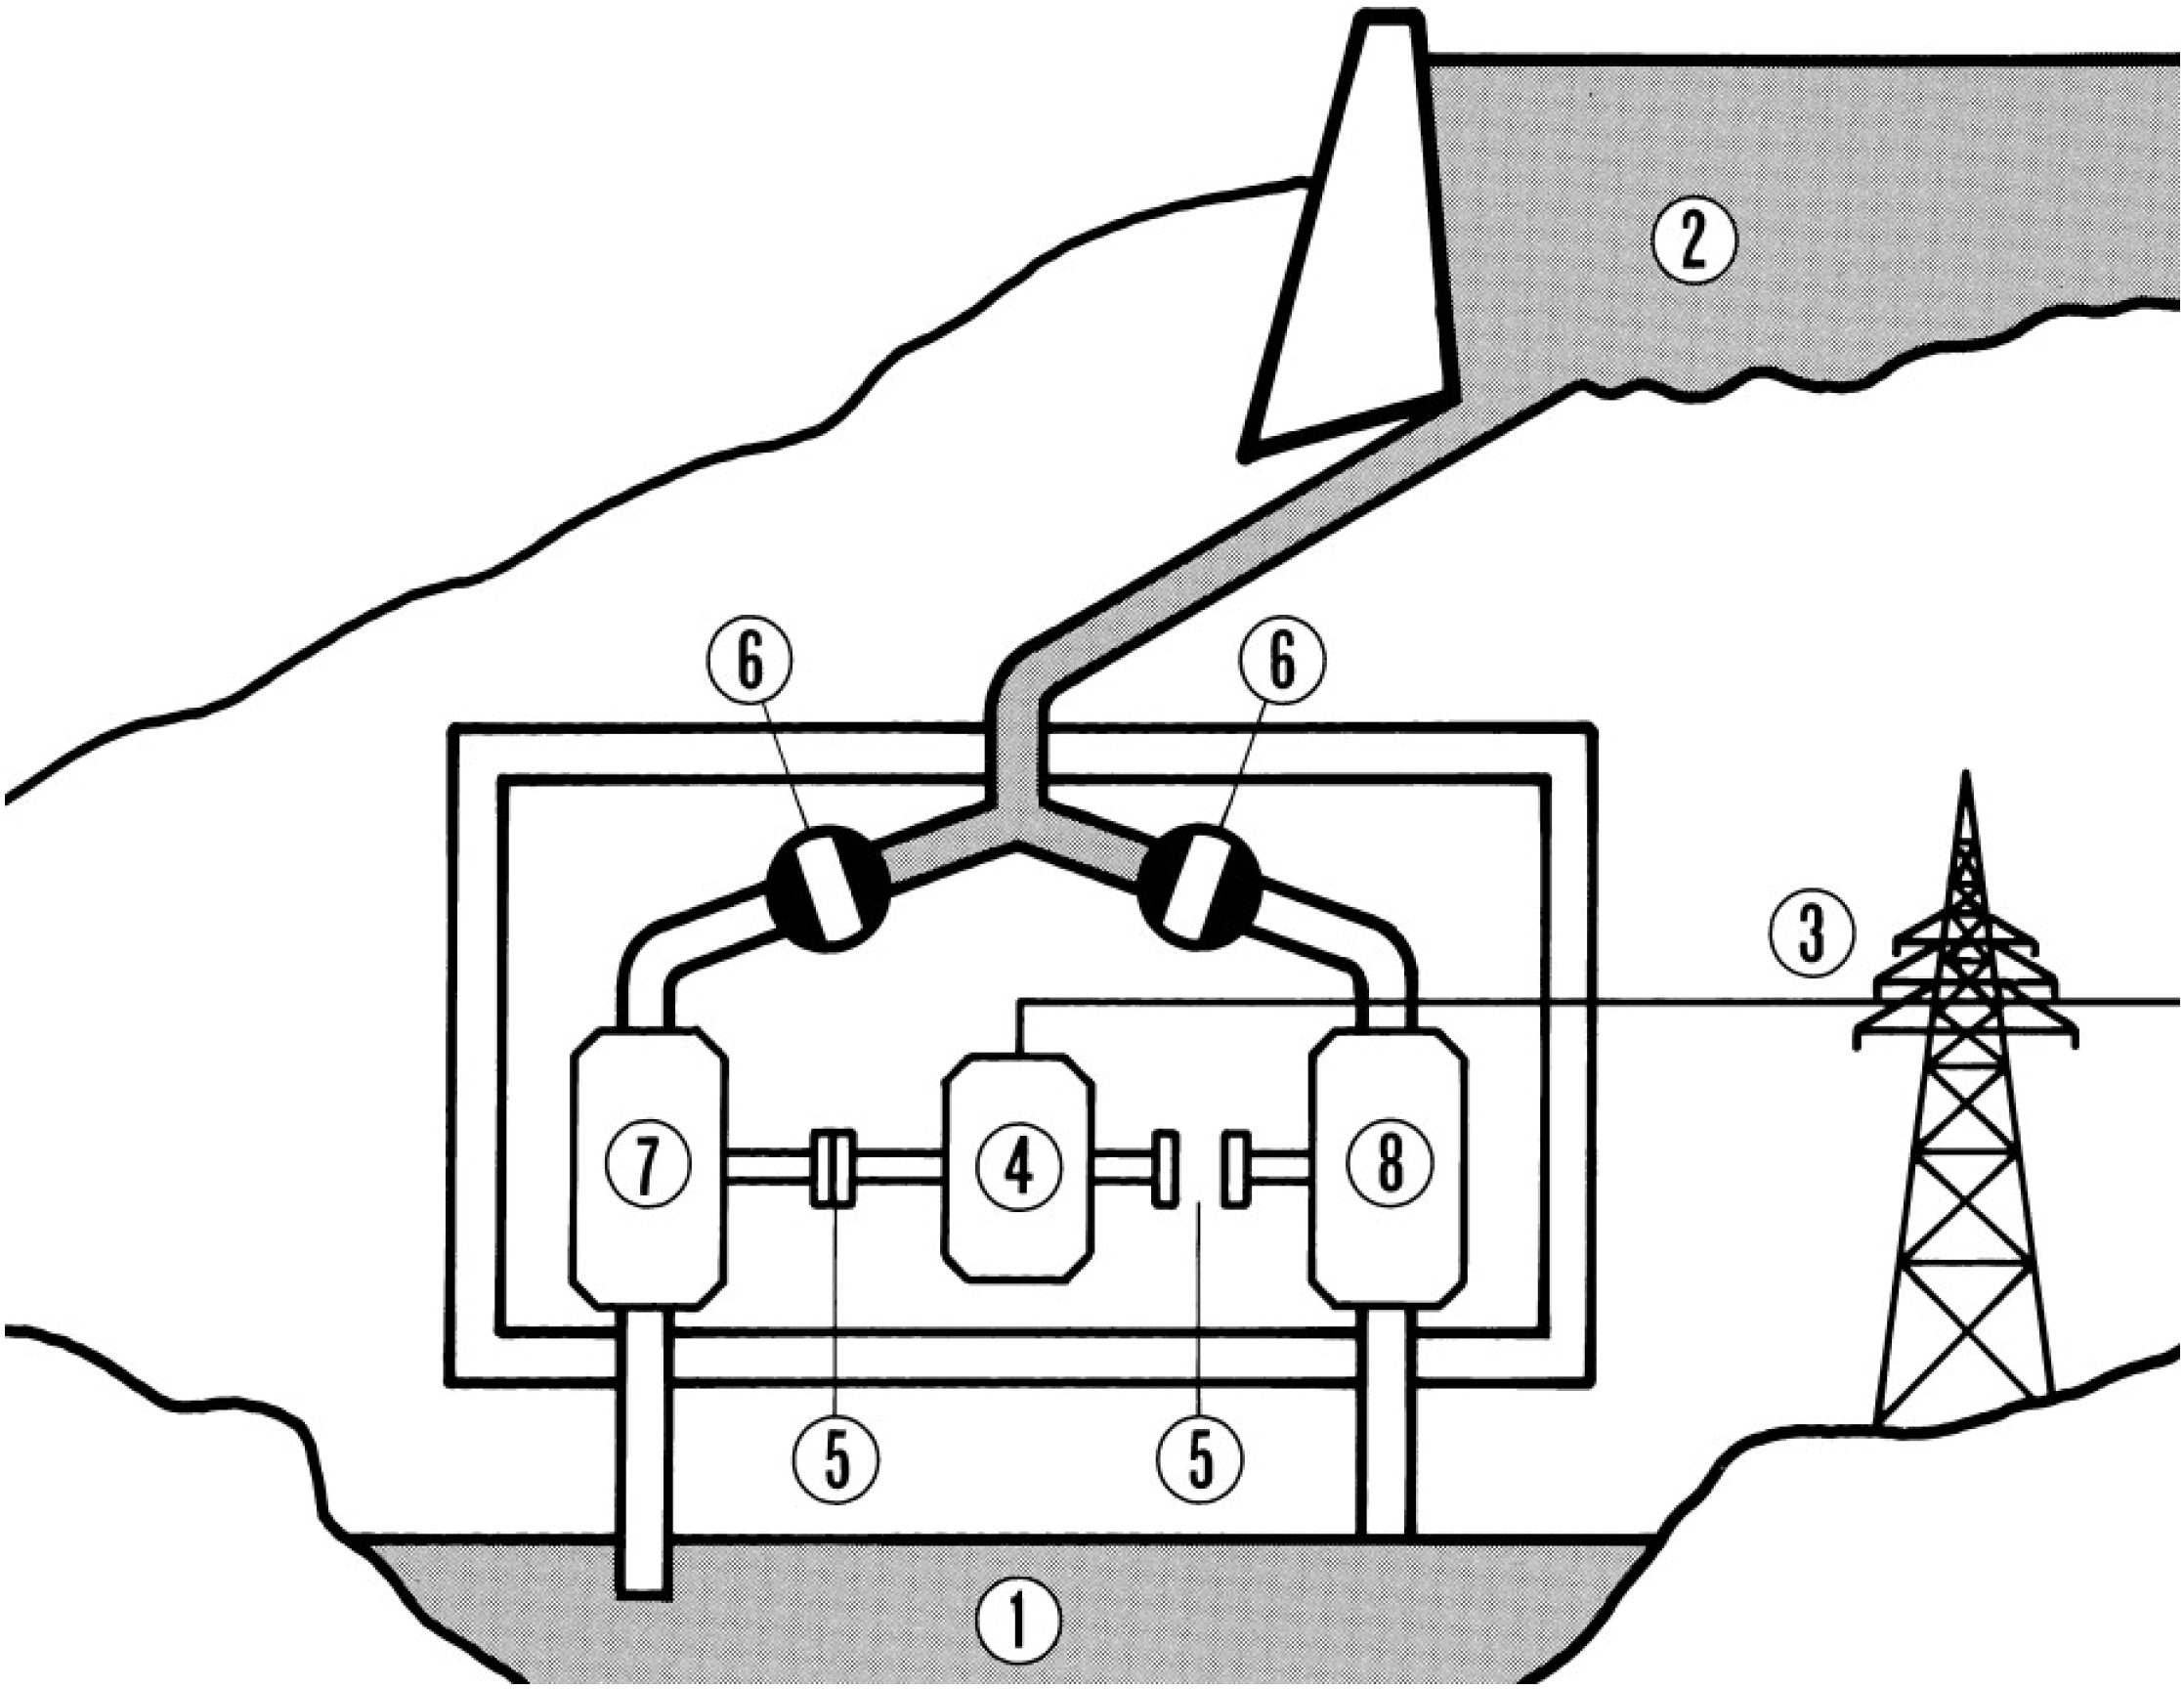
\includegraphics[width=0.95\columnwidth]{images/Pumpspeicherkraftwerke.png}
        \end{center}
    \end{minipage}
    \hfill
    \begin{minipage}[c]{0.29\columnwidth}
        \begin{enumerate}
            \item Unteres Becken
            \item Oberes Becken
            \item Energieableitung, Stromleitung
            \item Motorgenerator
            \item Kupplung
            \item Kugelschieber
            \item Pumpe
            \item Turbine
        \end{enumerate}
    \end{minipage}

    Wirkungsgrad der PSW: 65 – 80\%

\subsubsection{Maschinensatz}
    \begin{tabular}{c c}
        Zweimaschinensatz:  & Motor/Generator und Pumpturbine \\
        Dreimaschinenesatz: & Motor/Generator, Turbine und Pumpe
    \end{tabular}

\subsection{Hochdruck- (Speicher-) Anlagen}
    \begin{minipage}[c]{0.6\columnwidth}
        \begin{center}
            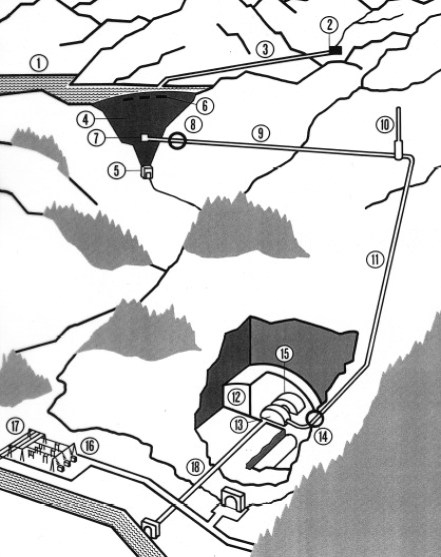
\includegraphics[width=0.95\columnwidth]{images/Hochdruckspeicheranlagen.png}
        \end{center}
    \end{minipage}
    \hfill
    \begin{minipage}[c]{0.39\columnwidth}
        \begin{enumerate}
            \item Stausee
            \item Wasserfassung
            \item Freispiegelstollen 
            \item[] (keine Druckleitung)
            \item Staumauer
            \item Grundablass (für kontr. Ablauf)
            \item Hochwasserentlastung (Überlauf)
            \item Einlauf
            \item Drosselklappe (Wasserfluss Druckstollen steuern)
            \item Druckstollen
            \item Wasserschloss (Druckausgleich Änderung Wasserdurchfluss)
            \item Druckschacht
            \item Zentrale
            \item Turbine
            \item Kugelschieber
            \item Generator
            \item Energieableitung, Transformatoren
            \item Schaltanlage
            \item Unterwasserstollen
        \end{enumerate}
    \end{minipage}

    ab circa 50m Fallhöhe (> 5 bar Druck, bis weit über 100 bar möglich)

\subsubsection{Stollen und Schächte}
    \begin{tabular}{ll}
        Freispiegelstollen:         & flach, nicht voll gefüllt, Umgebungsdruck\\
        Druckstollen (Betonverkl.): & flach, voll gefüllt, Druck $>$ Umgebungsdr. , $v < 5\,\mathrm{m/s}$ \\
        Druckschacht (Stahlpanz.):  & steil, voll gefüllt, Druck $\gg$ Umgebungsdr. , $v < 9\,\mathrm{m/s}$ 
    \end{tabular}

\subsection{Wasserschloss}
    Das Wasserschloss ist ein nach oben offenes Gefäss.
    Im Druckstollen sind grosse Wassermassen vorhanden. Diese Wassermassen müssen:

    \begin{itemize}
        \item beim Anfahren der Maschinengruppen beschleunigt,
        \item beim Abstellen gebremst werden.
    \end{itemize}
    Das Wasserschloss dient als Puffer

    \begin{center}
        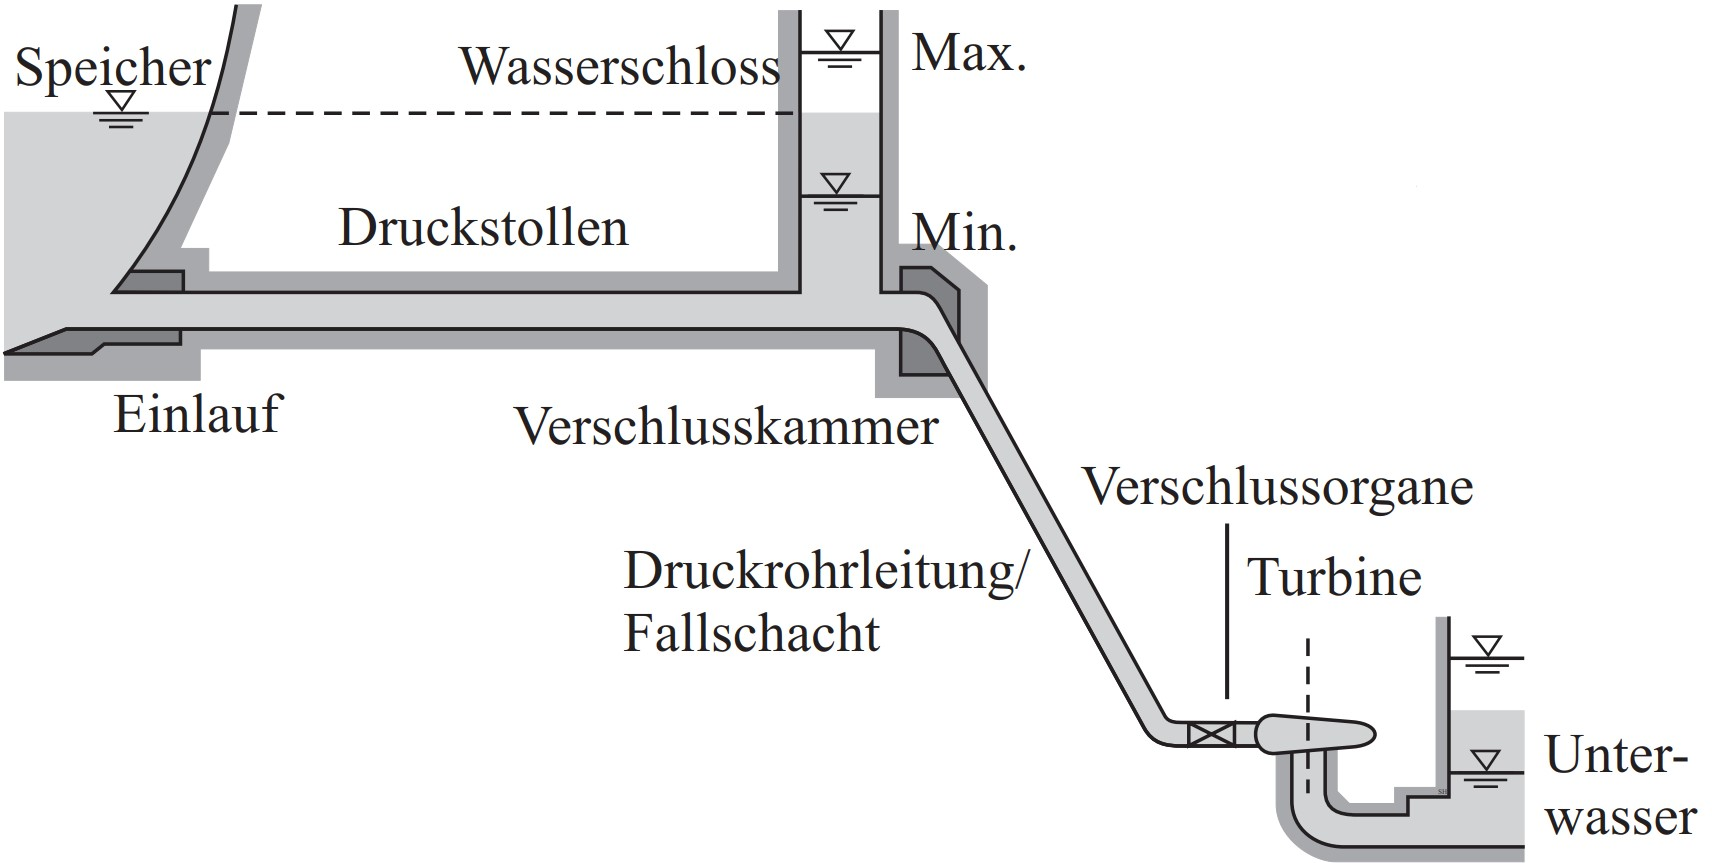
\includegraphics[width=0.6\columnwidth]{images/Wasserschloss.jpg}
    \end{center}

    \begin{minipage}[t]{0.33\columnwidth}
        \subsubsection{Generell}
        $
        \boxed{E_{\mathrm{ktot}} = E_{\mathrm{kSt}}+E_{\mathrm{ks}}} \\
        \boxed{E_{\mathrm{pot}} = E_{\mathrm{ktot}}} \\
        \boxed{h_{\mathrm{ws}} = \sqrt{\frac{E_{\mathrm{pot}} \cdot 2}{\rho_{\mathrm{w}} \cdot A_{\mathrm{ws}} \cdot g}}}
        $
    \end{minipage}%
    \hfill
    \begin{minipage}[t]{0.33\columnwidth}
        \subsubsection{Stollen}
        $
        \boxed{V_{\mathrm{St}} = l_{\mathrm{St}} \cdot A_{\mathrm{St}}}  \\
        \boxed{m_{\mathrm{wSt}} = \rho_{\mathrm{w}} \cdot V_{\mathrm{St}}} \\
        \boxed{v_{\mathrm{St}}= \frac{Q}{A_{\mathrm{St}}}} \\
        \boxed{E_{\mathrm{kSt}} = \frac{m_{\mathrm{wSt}} \cdot v_{\mathrm{St}}^2}{2}}
        $
    \end{minipage}%
    \hfill
    \begin{minipage}[t]{0.33\columnwidth}
        \subsubsection{Schacht}
        $
        \boxed{V_{\mathrm{s}} = l_{\mathrm{s}} \cdot A_{\mathrm{s}}} \\
        \boxed{m_{\mathrm{ws}} = \rho_{\mathrm{w}} \cdot V_{\mathrm{s}}} \\
        \boxed{v_{\mathrm{s}}= \frac{Q}{A_{\mathrm{s}}}} \\
        \boxed{E_{\mathrm{ks}} = \frac{m_{\mathrm{ws}} \cdot v_{\mathrm{s}}^2}{2}}
        $
    \end{minipage}

    \renewcommand{\arraystretch}{1.2}
    \begin{tabular}{@{} l p{7cm} l @{}}    
        $[A_{\mathrm{s}}]$      & Schachtfläche \dotfill                                        & $\mathrm{m^2}$ \\
        $[A_{\mathrm{St}}]$     & Stollenfläche \dotfill                                        & $\mathrm{m^2}$ \\
        $[A_{\mathrm{ws}}]$     & Wasserschlossfläche \dotfill                                  & $\mathrm{m^2}$ \\
        $[g]$                   & Fallbeschleunigung $(9.81\, \mathrm{m/s^2})$ \dotfill         & $\mathrm{m^2}$ \\
        $[h_{\mathrm{ws}}]$     & Höhe des Wasserspiegels im Wasserschloss \dotfill             & $\mathrm{m^2}$ \\
        $[l_{\mathrm{s}}]$      & Schachtlänge \dotfill                                         & $\mathrm{m}$ \\
        $[l_{\mathrm{St}}]$     & Stollenlänge \dotfill                                         & $\mathrm{m}$ \\
        $[m_{\mathrm{ws}}]$     & Wassermasse im Schacht \dotfill                               & $\mathrm{kg}$ \\
        $[m_{\mathrm{wSt}}]$    & Wassermasse im Stollen \dotfill                               & $\mathrm{kg}$ \\
        $[Q]$                   & Druchfluss \dotfill                                           &$\mathrm{m^3/s}$\\
        $[\rho_{\mathrm{w}}]$   & Dichte des Wassers ($1000\, \mathrm{kg/m^3}$) \dotfill        & $\mathrm{kg/m^3}$ \\
        $[V_{\mathrm{s}}]$      & Schachtvolumen \dotfill                                       & $\mathrm{m^3}$ \\
        $[V_{\mathrm{St}}]$     & Stollenvolumen \dotfill                                       & $\mathrm{m^3}$ \\
        $[v_{\mathrm{s}}]$      & Fliessgeschwindigkeit im Schacht\dotfill                      & $\mathrm{m/s}$ \\
        $[v_{\mathrm{St}}]$     & Fliessgeschwindigkeit im Stollen \dotfill                     & $\mathrm{m/s}$ \\
        $[E_{\mathrm{ks}}]$     & Kinetische Energie im Schacht \dotfill                        & $\mathrm{J}$\\
        $[E_{\mathrm{kSt}}]$    & Kinetische Energie im Stollen \dotfill                        & $\mathrm{J}$\\
        $[E_{\mathrm{pot}}]$    & Potentielle Energie           \dotfill                        & $\mathrm{J}$\\
    \end{tabular}
    \newcolumn

\subsection{Gezeitenkraftwerke}
    \begin{itemize}
        \item Nutzung des Tidenhubs
        \item Früher meist mit Staudammbauweise (hohe Umwelteinwirkungen)
        \item Heute meist Meeresströmungs-Kraftwerk
        \item Grösste Europäische Anlage in Frankreich (240 MW)
    \end{itemize}


\subsection{Wellenkraftwerk}
    \subsubsection{Wellenkraftwerk mit Pneumatischer Kammer}
    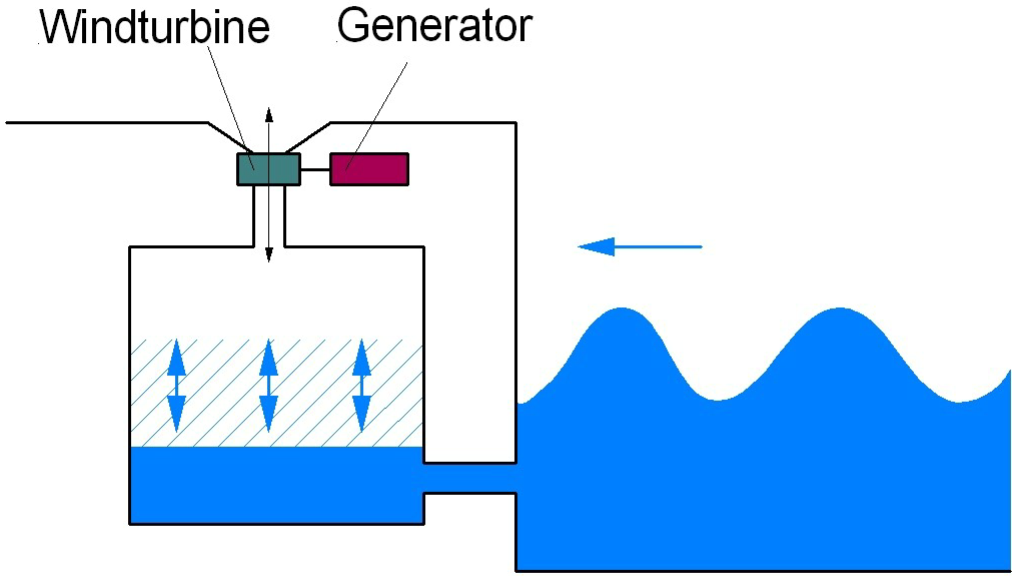
\includegraphics[width=0.55\columnwidth]{images/Wellenkraft mit Pneumatischer Kammer.png}

    \subsubsection{Wellenkraftwerk mit Rampe}
    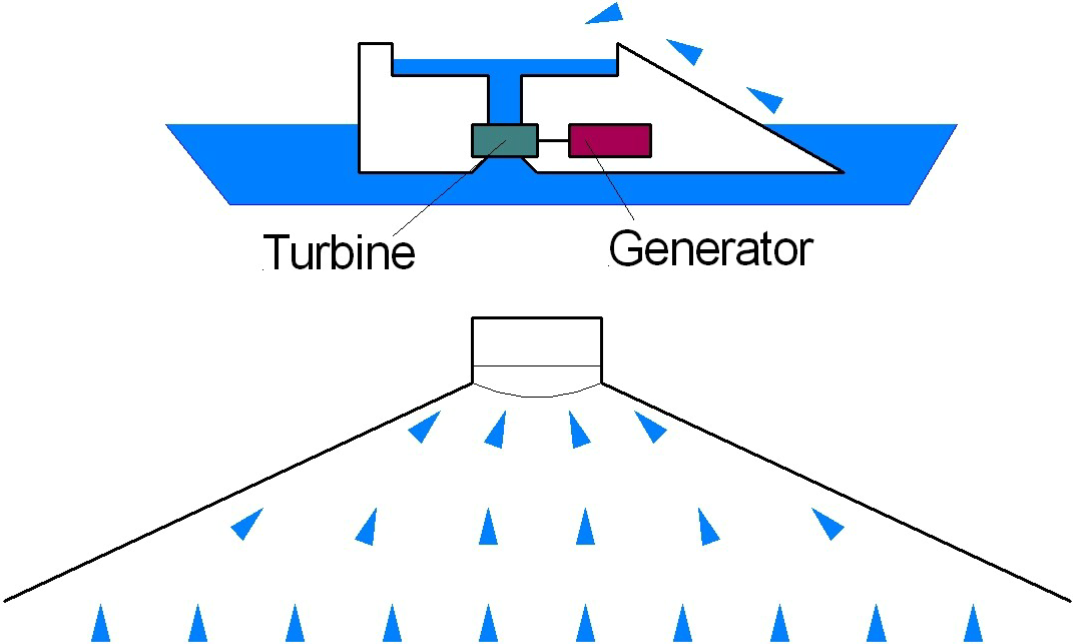
\includegraphics[width=0.55\columnwidth]{images/Wellenkraft mit Rampe.png} % done
        \section{Kenngrössen Turbinen}
\subsection{Hydraulische Leistung}
    \begin{minipage}[t]{0.35\columnwidth}\vspace*{-2mm}
        $\boxed{P_{\text{hyd}} = \rho \cdot Q \cdot g \cdot H_n}$
    \end{minipage}%
    \hfill
    \begin{minipage}[t]{0.64\columnwidth}\vspace*{-2mm}
        \renewcommand{\arraystretch}{1.1}
        \begin{tabular}{@{} l p {3.6cm} l @{}}
            $[P_{\text{hyd}}]$  & Hydraulische Leistung \dotfill & $\mathrm{W}$ \\
            $[Q]$               & Nutzwassermenge \dotfill & $\mathrm{\frac{m^3}{s}}$ \\
            $[H_n]$             & Nettofallhöhe \dotfill & $\mathrm{m}$ \\
            $[\rho]$            & Dichte des Wassers ($\rho = 1000$) \dotfill & $\mathrm{\frac{kg}{m^3}}$ \\
            $[g]$               & Erdbeschleunigung ($g = 9.81$) \dotfill & $\mathrm{\frac{m}{s^2}}$ \\
        \end{tabular}
    \end{minipage}

\subsection{Mechanische Leistung an der Turbinenwelle}
    \begin{minipage}[t]{0.35\columnwidth}\vspace*{-2mm}
        $\boxed{P_{\text{mech}} = \omega \cdot M = \eta_t \cdot P_{\text{hyd}}}$
    \end{minipage}%
    \hfill
    \begin{minipage}[t]{0.64\columnwidth}\vspace*{-2mm}
        \renewcommand{\arraystretch}{1.2}
        \begin{tabular}{@{} l p {3.6cm} l @{}}
            $[P_{\text{mech}}]$  & Mechanische Leistung   \dotfill & $\mathrm{W}$ \\
            $[\omega]$           & Winkelgeschwindigkeit \dotfill & $\mathrm{\frac{rad}{s}}$ \\
            $[\eta_t]$           & Wirkungsgrad Turbine \dotfill & $-$ \\
            $[M]$                & Drehmoment            \dotfill & $\mathrm{Nm}$ \\
        \end{tabular}
    \end{minipage}
% \subsection{Winkelgeschwindigkeit}
%     \begin{minipage}[t]{0.29\columnwidth}\vspace*{-2mm}
%         $\boxed{P_{\text{mech}} = \omega \cdot M = \eta_t \cdot P_{\text{hyd}}}$
%     \end{minipage}%
%     \hfill
%     \begin{minipage}[t]{0.7\columnwidth}\vspace*{-2mm}
%         \renewcommand{\arraystretch}{1.2}
%         \begin{tabular}{@{} l p {3.5cm} l @{}}
%             $[P_{\text{mech}}]$  & Mechanische Leistung   \dotfill & $\mathrm{W}$ \\
%             $[\omega]$           & Winkelgeschwindigkeit \dotfill & $\mathrm{\frac{rad}{s}}$ \\
%             $[\eta_t]$           & Wirkungsgrad Turbine \dotfill & $-$ \\
%             $[M]$                & Drehmoment            \dotfill & $\mathrm{Nm}$ \\
%         \end{tabular}
%     \end{minipage}
%     $\boxed{\omega = 2 \cdot \pi \cdot n}$

%     \vspace{0.15cm}

%     \renewcommand{\arraystretch}{1.2} % Erhöht Zeilenhöhe für bessere Lesbarkeit
%     \begin{tabular}{@{} l p {6cm} l @{}}
%         $[\omega]$  & Winkelgeschwindigkeit \dotfill & $\mathrm{\frac{rad}{s}}$ \\
%         $[n]$       & Drehzahl              \dotfill & $\mathrm{\frac{1}{s}}$ \\
%     \end{tabular}

\subsection{Betriebszustände der Maschinengruppe}
    \textbf{(Maschinengruppe = Turbine/Pumpe + Generator/Motor)}

    \begin{itemize}
        \item Inselbetrieb
        \item Parallelbetrieb, Verbundbetrieb
        \item Instationäre Vorgänge
        \begin{itemize}
            \item Anfahren und Abstellen
            \item Lastabwurf $\Rightarrow$ Überdrehzahl
        \end{itemize}
    \end{itemize}

    \textbf{Durchgangsdrehzahl $n_D$} (auch Schleuderdrehzahl genannt)

    $\Rightarrow$ höchste erreichbare Drehzahl ohne Last (z.B. bei Versagen des Generators)

    Die Durchgangsdrehzahl ist eine Bemessungsgröße. 

    Die Maschinengruppe darf bei der Durchgangsdrehzahl keinen Schaden erleiden.

\subsection{Spezifische Drehzahl $n_q$}
    \begin{minipage}[t]{0.35\columnwidth}\vspace*{-2mm}
        $\boxed{n_q = n \cdot \frac{\sqrt{Q}}{H_n^{3/4}}}$
    \end{minipage}%
    \hfill
    \begin{minipage}[t]{0.64\columnwidth}\vspace*{-2mm}
        \renewcommand{\arraystretch}{1.2}
        \begin{tabular}{@{} l p {3.6cm} l @{}}
            $[n_q]$  & Spezifische Drehzahl \dotfill  & $\text{U/min}$ \\
            $[n]$    & Drehzahl der Turbine \dotfill  & $\text{U/min}$ \\
            $[Q]$    & Nutzwassermenge \dotfill       & $\frac{\text{m}^3}{\text{s}}$ \\
            $[H_n]$  & Nettofallhöhe \dotfill         & $\text{m}$ \\
        \end{tabular}
    \end{minipage}

    $n_q$ ist die Drehzahl einer Turbine in \(\mathrm{U/min}\), 
    welche bei einem Gefälle von \(1 \,\mathrm{m}\) einen Volumenstrom 
    von \(1 \,\mathrm{m}^3/\mathrm{s}\) aufweist (Ähnlichkeitsgesetz).

\subsubsection{Typische $n_q$}
    \textbf{Peltonturbinen} \hspace{1cm} $<$ 20 U/min 

    \vspace{0.15cm}

    \textbf{Francisturbinen} \hspace{1cm} ca. 20 bis ca. 100 U/min 

    \vspace{0.15cm}

    \textbf{Kaplanturbinen} \hspace{1cm} $>$ 100 U/min

\section{Turbinen}
    \begin{minipage}[t]{0.49\columnwidth}
        Aktionsturbinen:
            \begin{itemize}
                \item Peltonturbinen
                \item Durchströmturbinen
            \end{itemize}
    \end{minipage}%
    \hfill
    \begin{minipage}[t]{0.49\columnwidth}
        Reaktionsturbinen:
        \begin{itemize}
            \item Francisturbinen
            \item Kaplanturbinen
            \item Rohrturbinen
            \item Kreiselpumpen als Turbinen
        \end{itemize}
    \end{minipage}

\subsection{Peltonturbine}
    \begin{minipage}[c]{0.4\columnwidth}
        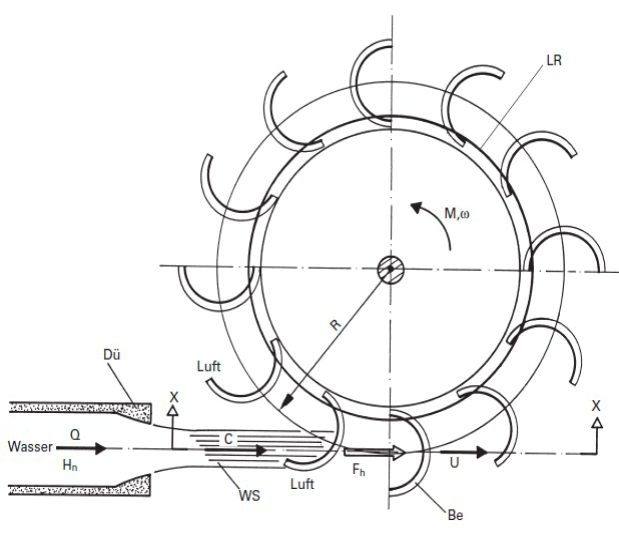
\includegraphics[width=0.98\columnwidth]{images/Pelton_Turbine_1.png}    
    \end{minipage}%
    \hfill
    \begin{minipage}[c]{0.4\columnwidth}
        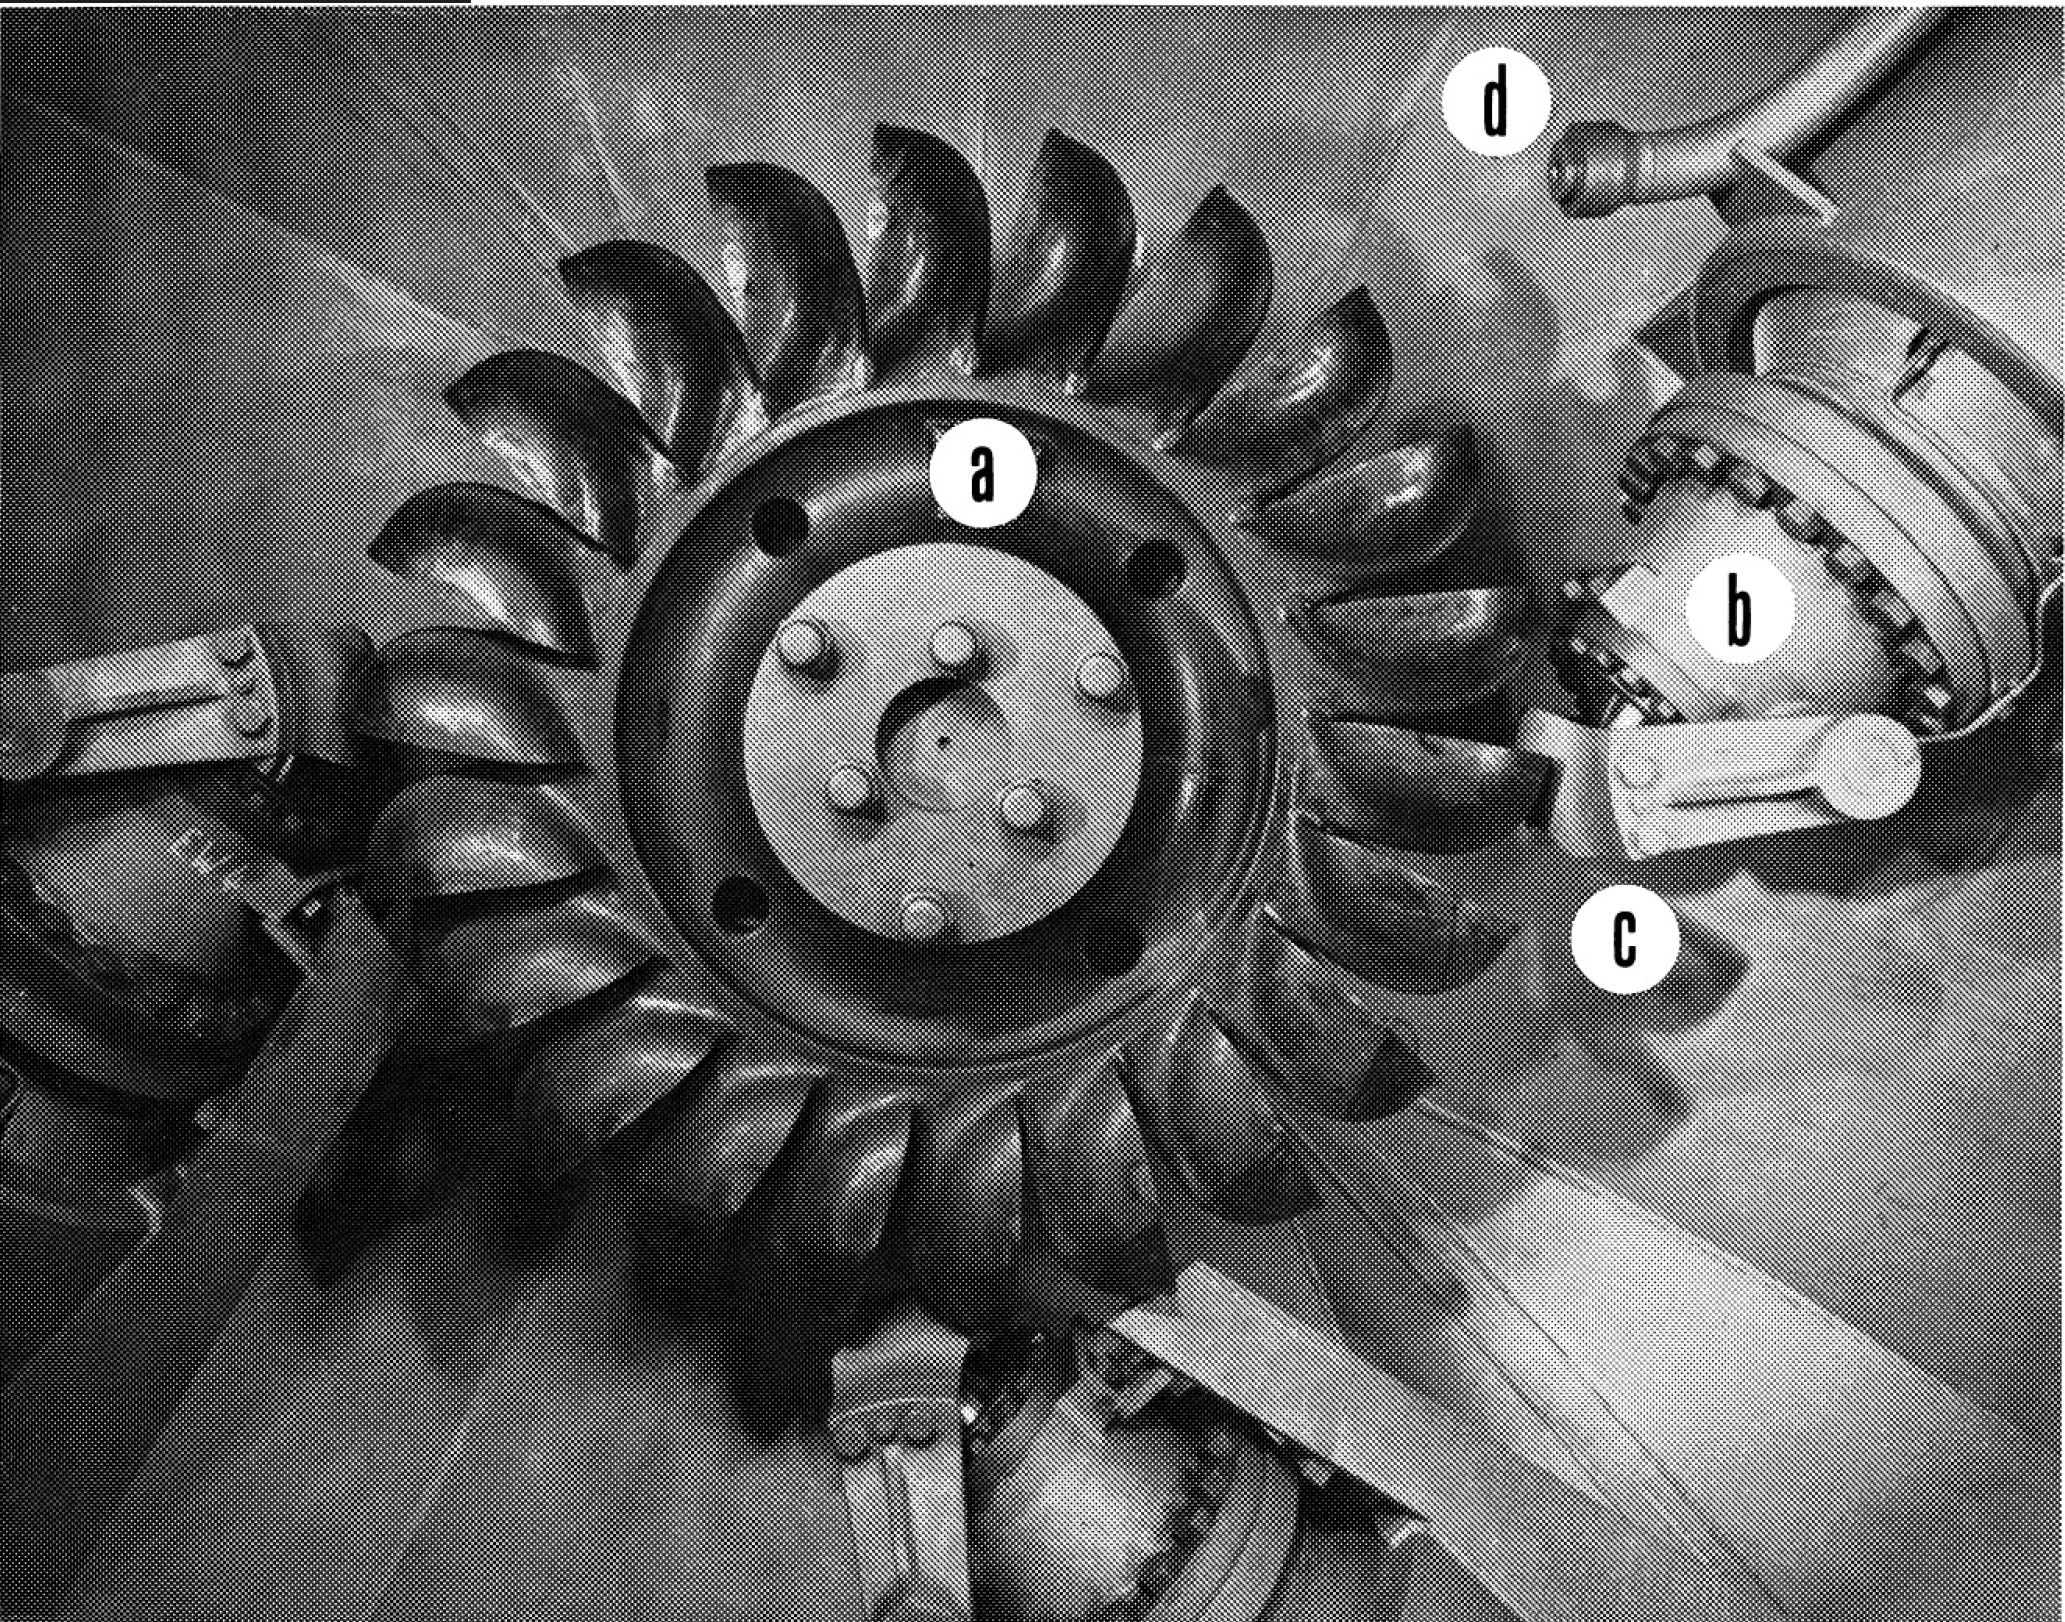
\includegraphics[width=0.98\columnwidth]{images/Pelton_Turbine_2.png}   
    \end{minipage}%
    \hfill
    \begin{minipage}[c]{0.2\columnwidth} 
        \begin{enumerate}[a)]
            \item Peltonrad
            \item Düse
            \item Strahlablenker
            \item Bremsdüse
        \end{enumerate}
    \end{minipage}

    \vspace{0.15cm}

    \begin{minipage}[c]{0.48\columnwidth}
        Düse offen    

        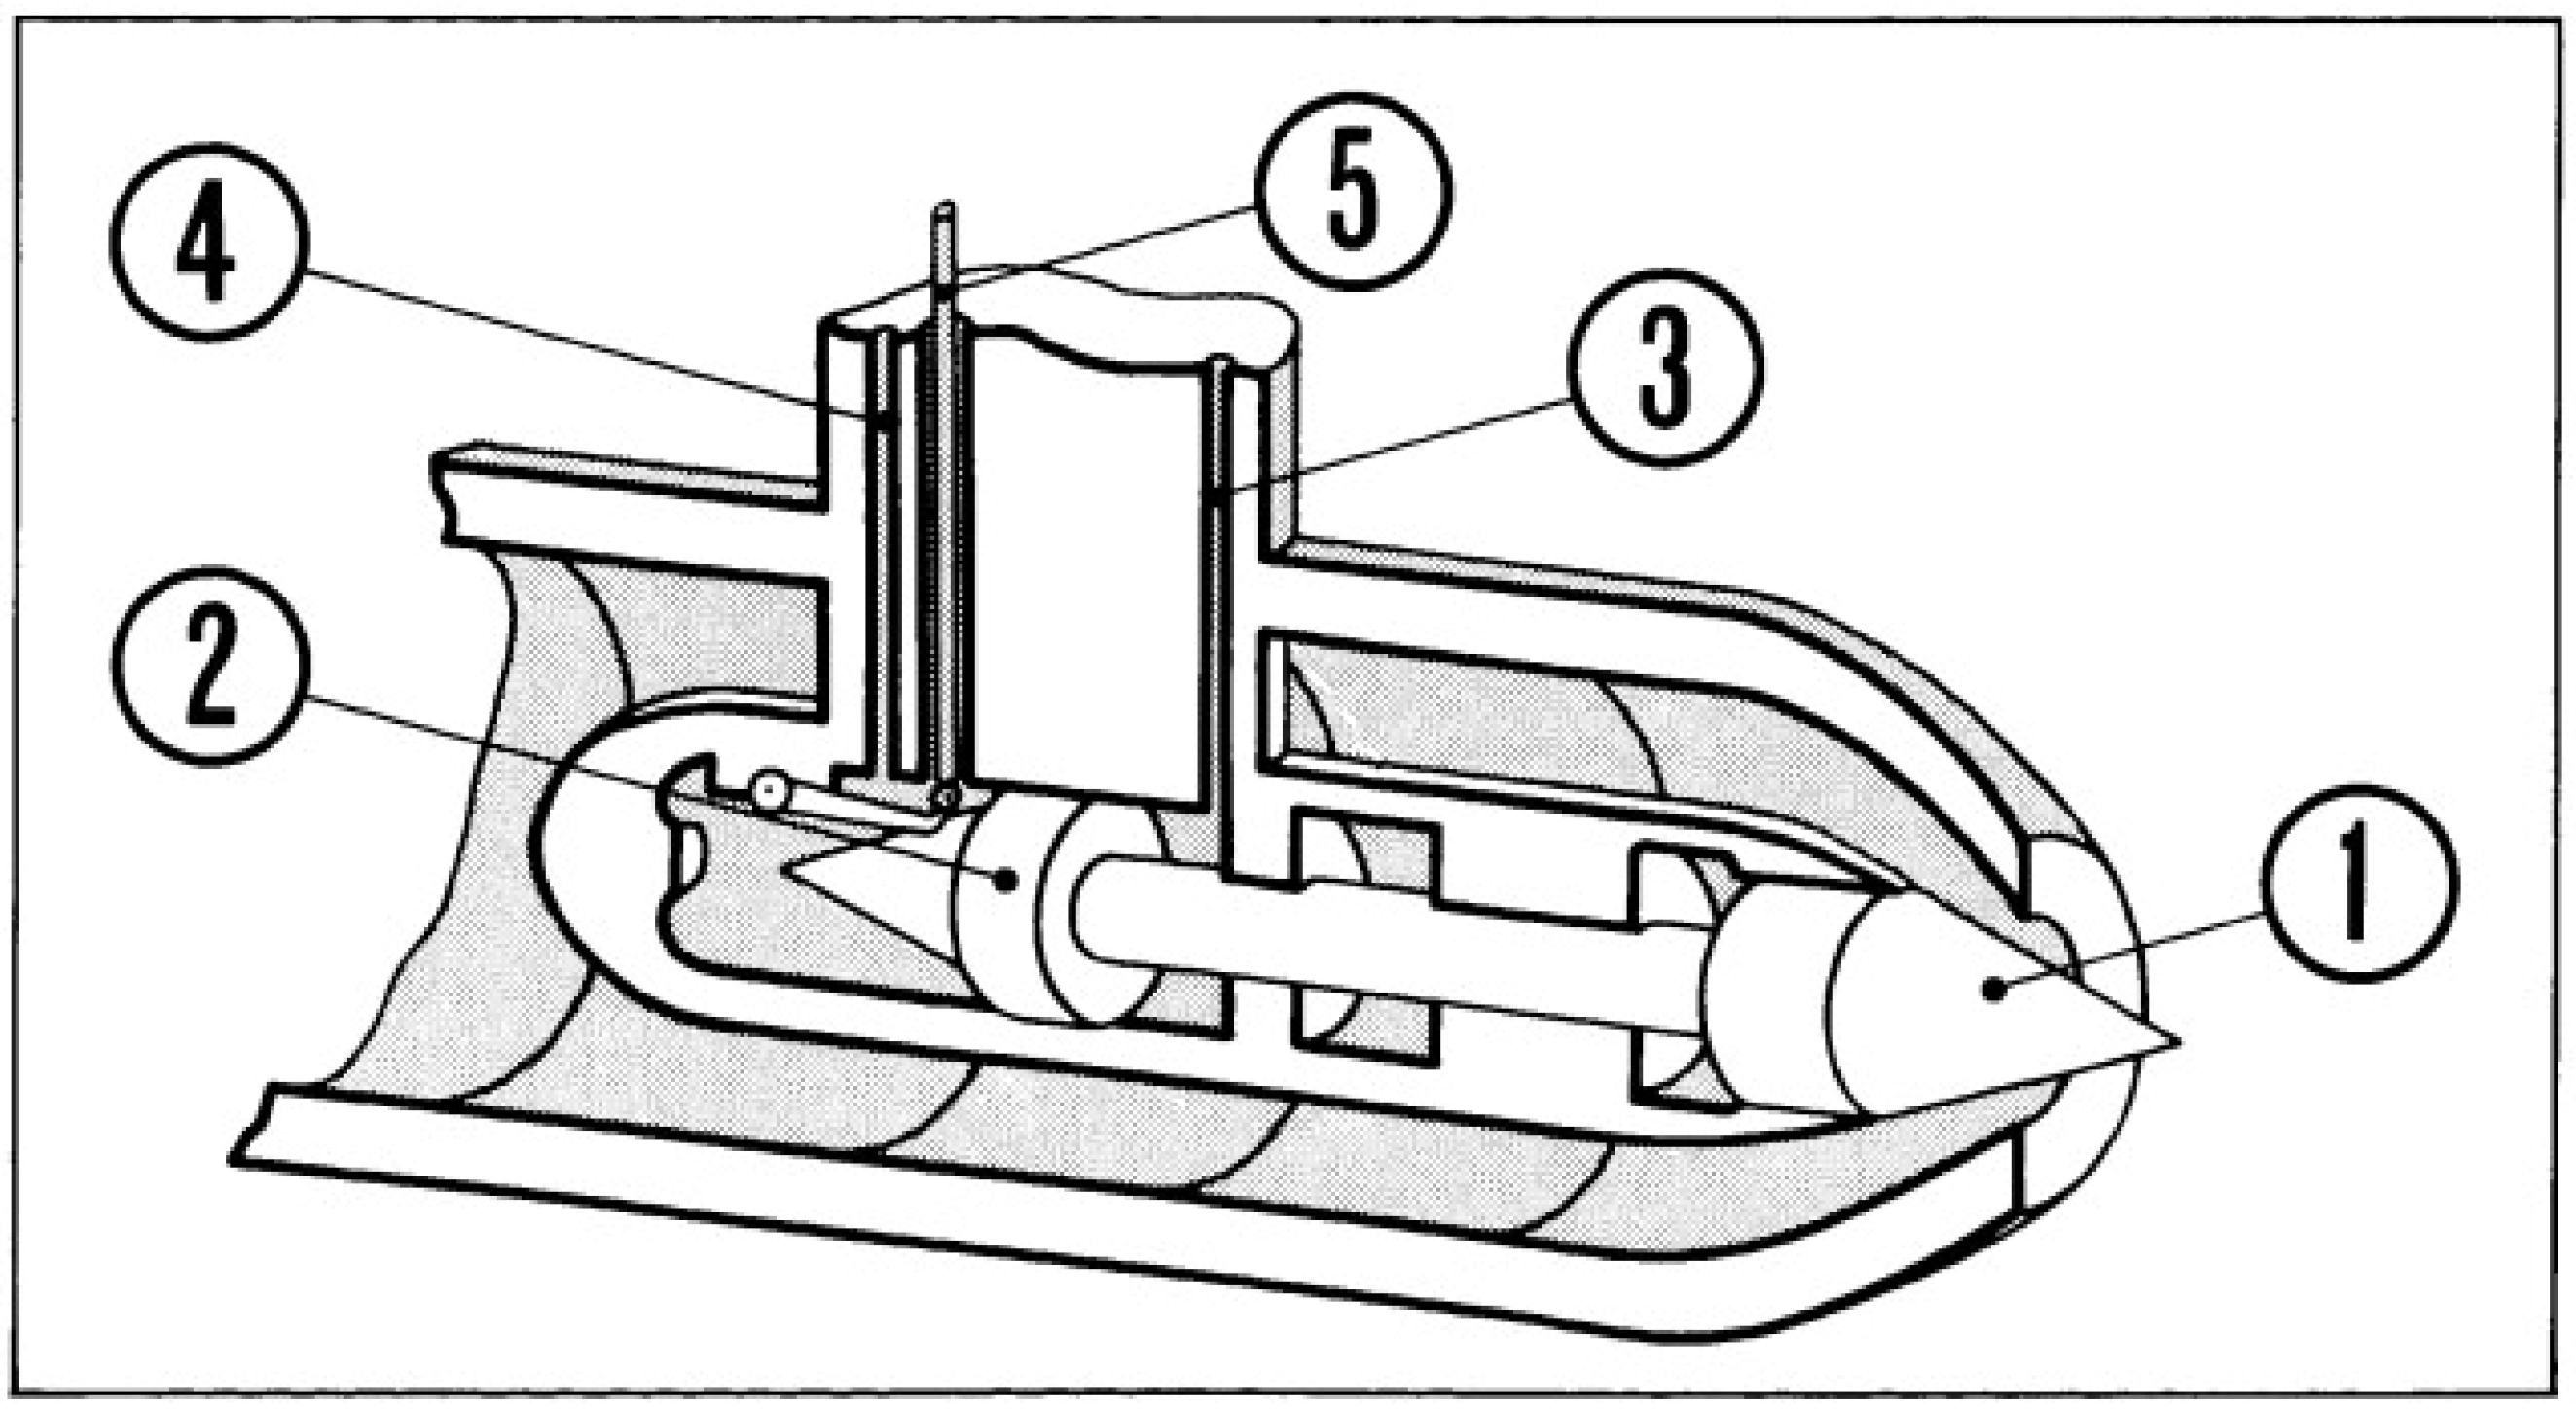
\includegraphics[width=0.98\columnwidth]{images/Pelton_Turbine_Düse_offen.png}    
    \end{minipage}
    \hfill
    \begin{minipage}[c]{0.48\columnwidth}
        Düse geschlossen   

        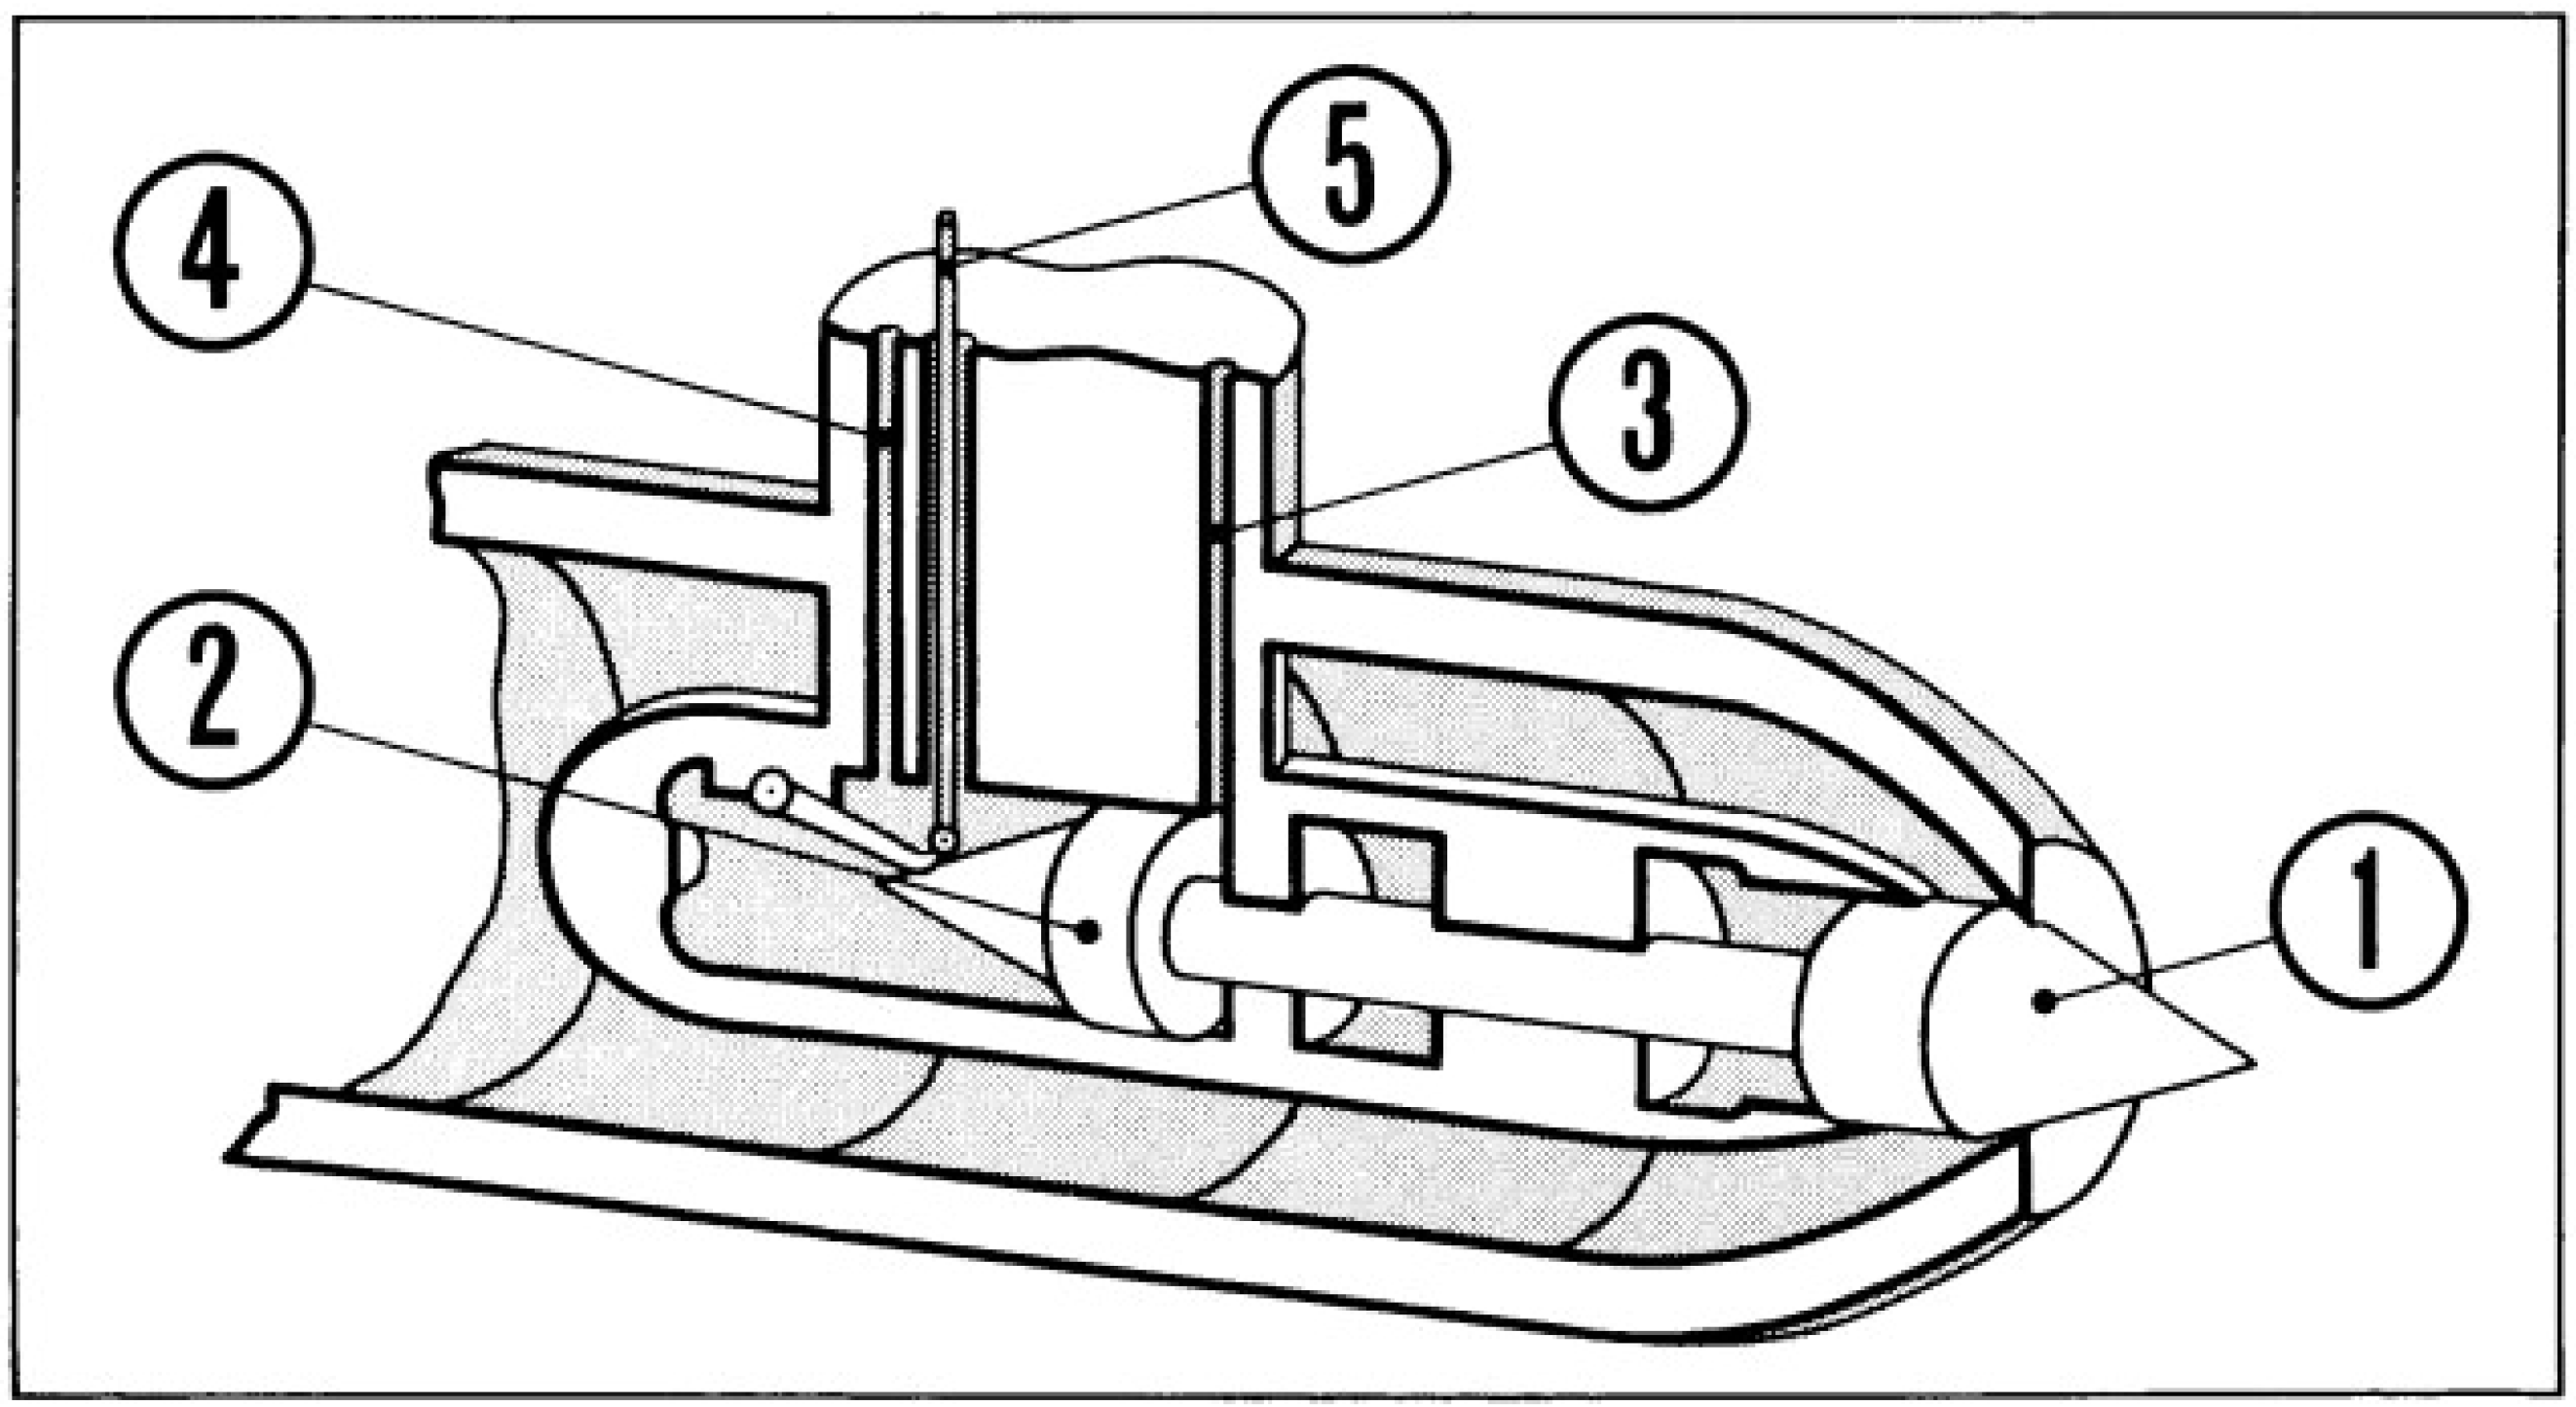
\includegraphics[width=0.98\columnwidth]{images/Pelton_Turbine_Düse_geschlossen.png}   
    \end{minipage}

    \vspace{-4mm}
    \def\columnseprulecolor{\color{white}}
    \begin{enumerate}
        \begin{multicols}{2}
            \item Düsennadel
            \item Kolben
            \item Öl zum öffnen
            \item Öl zum Schliessen
            \item Rückmeldung
        \end{multicols}
    \end{enumerate}
    \def\columnseprulecolor{\color{black}}

\subsubsection{Eingenschaften und Merkmale}
    \begin{itemize}
        \item Guter Wirkungsgrad über einen großen Einsatzbereich von 10 bis 100\% der max. Leistung
        \item Unkritische Maschine
        \item Der sogenannte Gletscherschliff muss beachtet werden (Erosion am Laufrad)
        \item Verschraubung Rad- / Generatorflansch (Kupplung) mit z.B. mechanisch vorgespannten Dehnschrauben
        \item Trockenenlegung der Kupplung
        \item Wirkungsgradverbesserungen oft möglich
        \item Rissen im Bereich der Becherwurzel (hochbelastete Zone) gilt ein spezielles Augenmerk
    \end{itemize}

    
\subsection{Reaktionsturbinen Funktionsprinzip}
    \begin{minipage}[t]{0.56\columnwidth}    
        \subsubsection{Turbinenspirale (TS)} 
            exzentrisch zur Turbinenachse angeordneter Zulaufkanal, der die durch eine \textbf{Turbinenspirale} erzeugte Drallströmung (\textbf{DS}) veranschaulicht (<<Badewannenablass>>)
        
        \subsubsection{Laufrad (LR)} 
            Schaufelrad, welches das in der \textbf{Drallströmung} DS platzierte Laufrad der Turbine darstellt
    \end{minipage}%
    \hfill
    \begin{minipage}[t]{0.43\columnwidth}
        \centering \vspace{-0.7\baselineskip}
        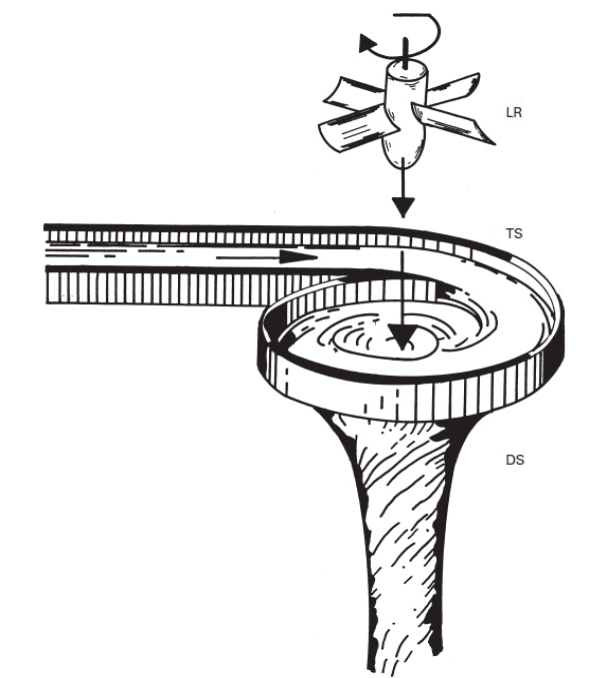
\includegraphics[width=0.9\columnwidth]{images/Laufradturbinen.png}  
    \end{minipage}
    
\subsubsection{Kavitation}
    \begin{minipage}[t]{0.65\columnwidth}
        \centering \vspace{-0.7\baselineskip}
        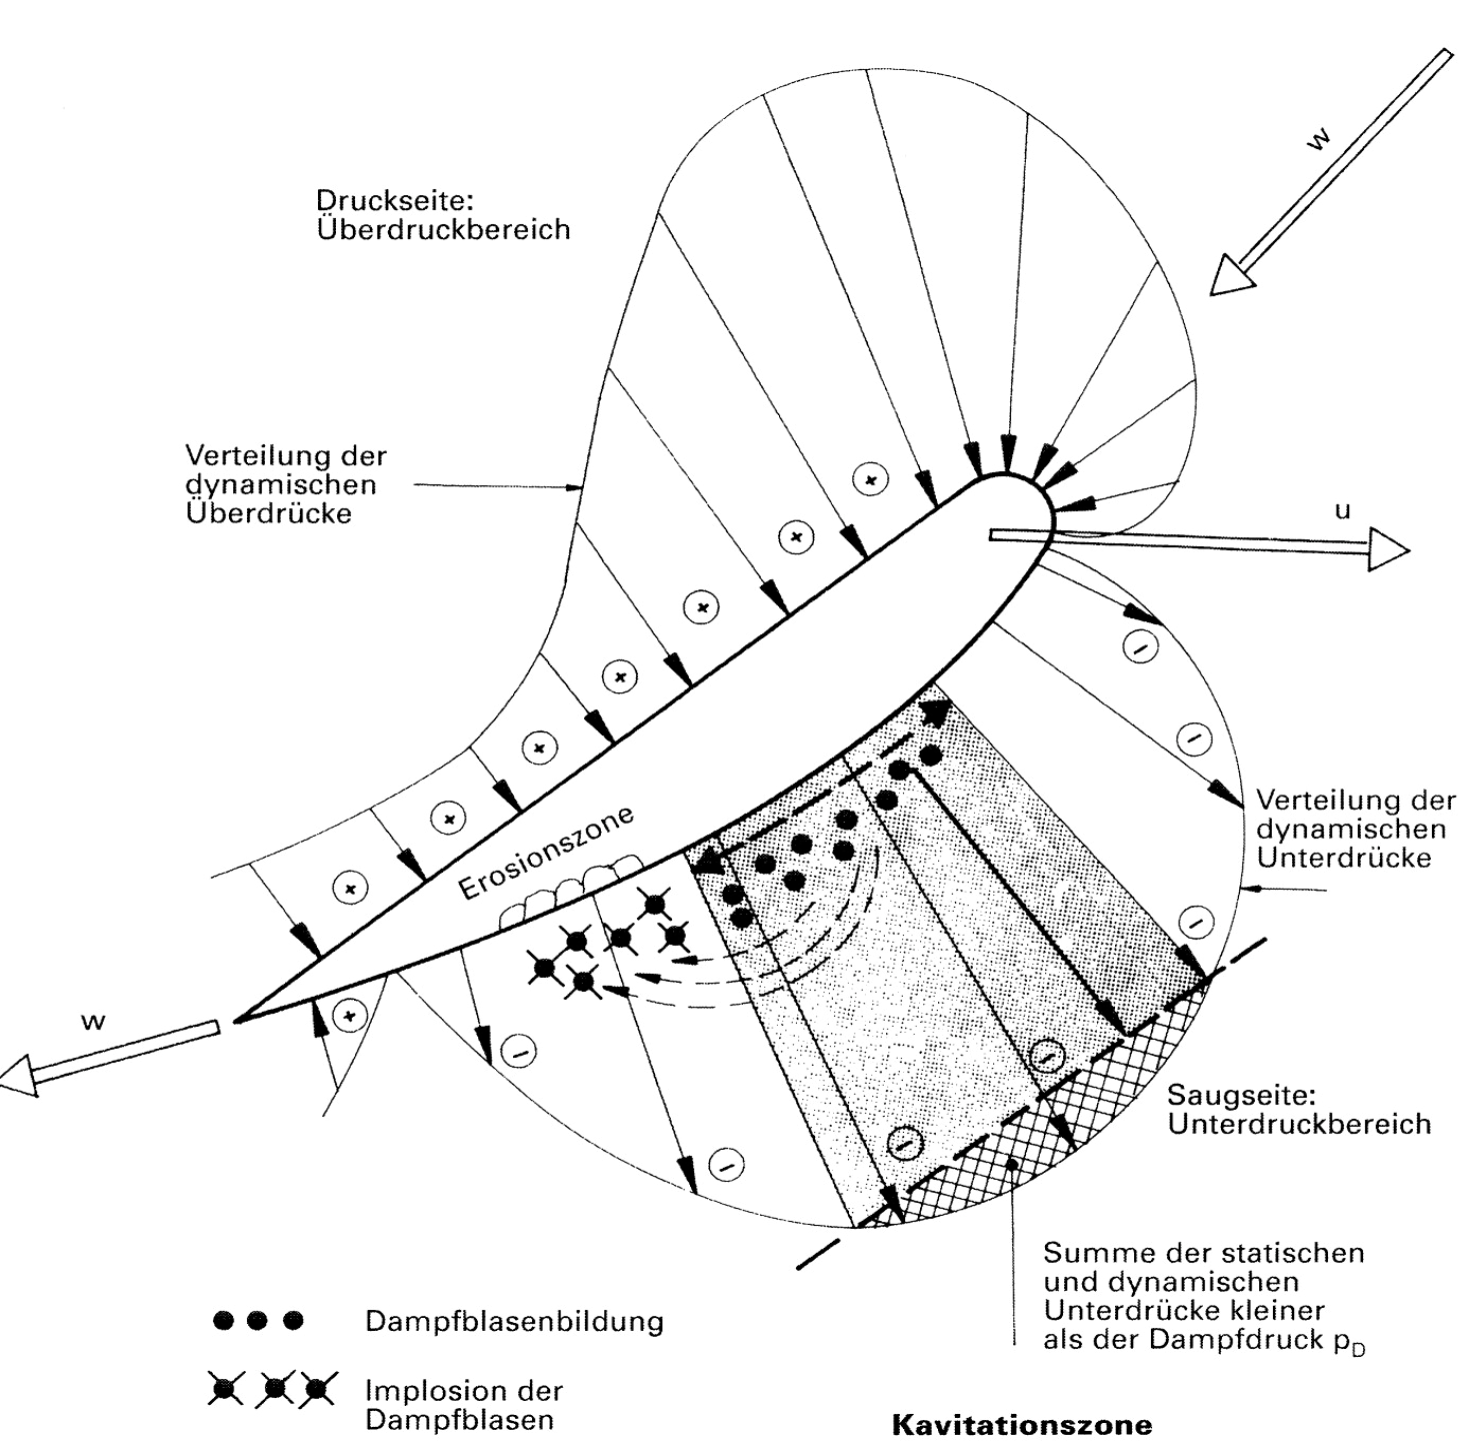
\includegraphics[width=0.95\linewidth]{images/Kavitation.png}
    \end{minipage}%
    \hfill
    \begin{minipage}[t]{0.34\columnwidth}
        \begin{itemize}
            \item[$w$] Rel. Geschw. des Wassers 
            \item[$u$] Umfanggeschw. der Schaufel
        \end{itemize}
    \end{minipage}  
    
    \vspace{0.15cm}
    
    \begin{tabular}{ll}
        \toprule[.13em]
        \textbf{Turbinentyp} & \({n_D}/{n_N}\) \\
        \midrule
        Francis, \(n_q = 40 \ldots 80\) U/min                       & \(1.7 \ldots 2.0\) \\
        Francis, \(n_q = 80 \ldots 120\) U/min                      & \(2.0 \ldots 2.2\) \\
        Propeller, feste Lauf- und Leitschaufeln                    & \(1.8 \ldots 2.2\) \\
        Kaplan, verstellbare Laufschaufeln, feste Leitschaufeln     & \(2.4 \ldots 2.8\) \\
        Kaplan, verstellbare Lauf- und Leitschaufeln                & \(2.4 \ldots 3.2\) \\
        Pumpen im Turbinenbetrieb, \(n_q = 30 \ldots 100\) U/min    & \(1.4 \ldots 1.8\) \\
        \bottomrule[.13em]
    \end{tabular}
    
    \vspace{0.15cm}
    
    Je grösser \({n_D}/{n_N}\), desto stärker muss die Turbine dimensioniert werden
    
    \newcolumn
    
    \textbf{Verhältnis der Volumenströme bei Durchgangs- bzw. Nenndrehzahl:}

    \begin{minipage}[t]{0.49\columnwidth}
        $\begin{aligned}
            n_q < 100 \ \mathrm{U/min:} & \quad Q_D < Q_N \\
            n_q = 100 \ \mathrm{U/min:} & \quad Q_D = Q_N \\
            n_q > 100 \ \mathrm{U/min:} & \quad Q_D > Q_N 
        \end{aligned}$
    \end{minipage}%
    \hfill
    \begin{minipage}[t]{0.49\columnwidth}
        \begin{itemize}
            \item \textbf{Durchgangsdrehzahl} \(n_D\)
            \item \textbf{Nenndrehzahl} \(n_N\)
            \item \textbf{Spezifische Drehzahl} \(n_q\)
        \end{itemize}
    \end{minipage}

    \renewcommand{\arraystretch}{1.2} % Erhöht Zeilenhöhe für bessere Lesbarkeit
    \begin{tabular}{@{} l p {7cm} l @{}}
        $[n_D]$   & Drehzahl bei Lastabwurf (plötzlicher Generatorverlust)  \dotfill & $\mathrm{\frac{U}{min}}$ \\
        $[n_N]$   & Tatsächliche Drehzahl im Normalbetrieb                    \dotfill & $\mathrm{\frac{U}{min}}$ \\
        $[n_q]$   & Drehzahl einer skalierten Maschine  \(\left(H = 1\,\mathrm{m},\, Q = 1\,\mathrm{m}^3/\mathrm{s}\right)\) \dotfill & $\mathrm{\frac{U}{min}}$ \\
    \end{tabular}
    
\subsection{Francisturbinen}
    \begin{minipage}[t]{0.48\columnwidth}
        \centering \vspace{-0.7\baselineskip}
        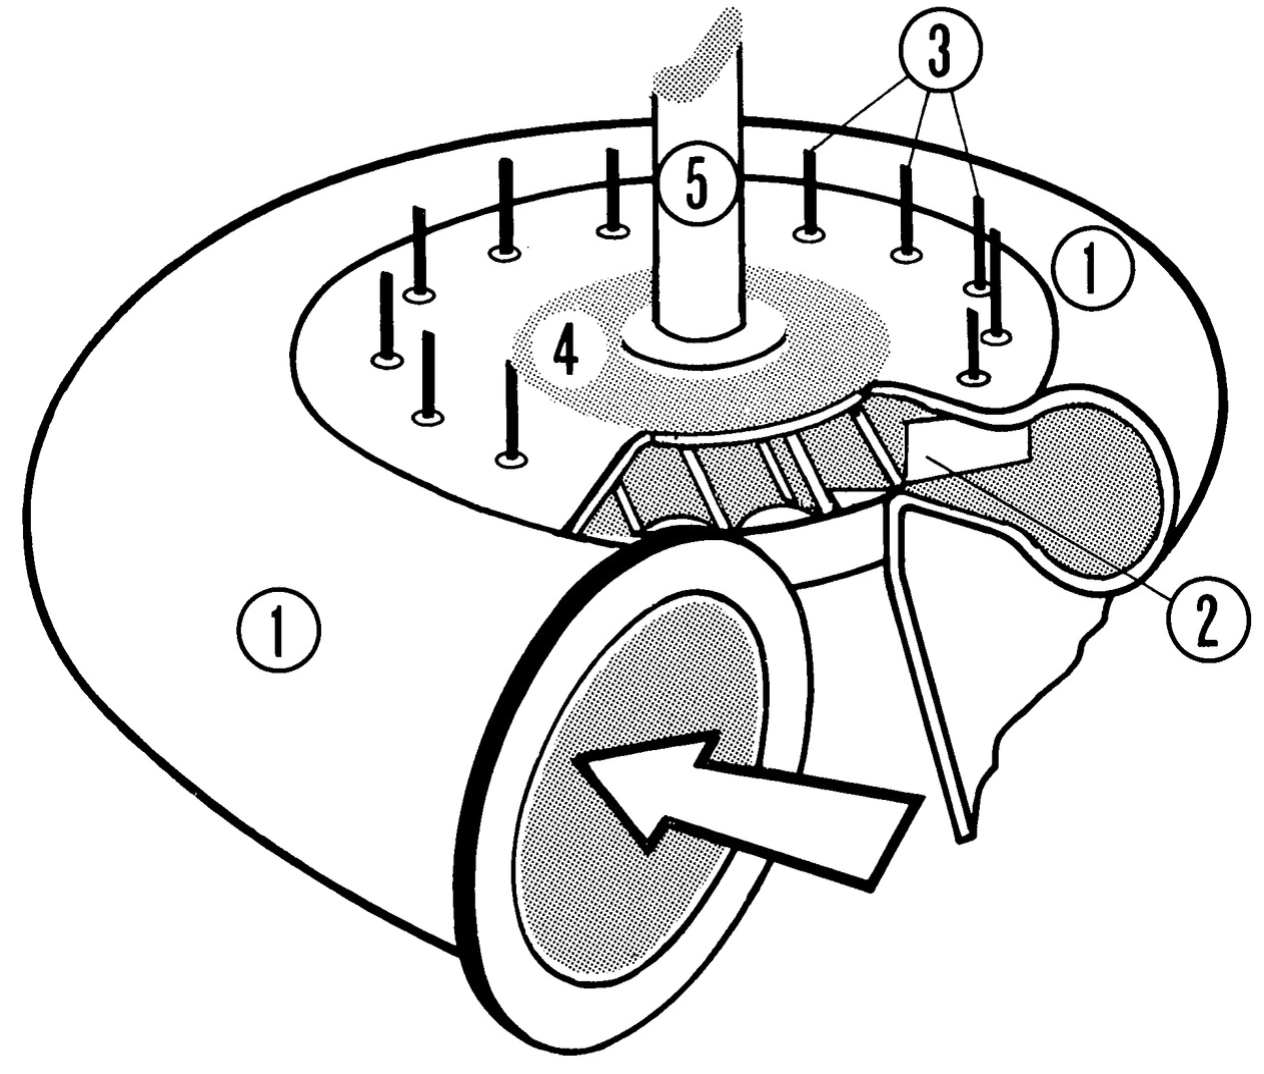
\includegraphics[width=0.85\columnwidth]{images/Francis_Turbine.png}    
    \end{minipage}
    \hfill
    \begin{minipage}[t]{0.48\columnwidth}
        \begin{enumerate}
            \item Einlaufspirale
            \item Leitschaufeln
            \item Leitschaufelnachse
            \item Laufrad
            \item Turbinenwelle
        \end{enumerate}  
    \end{minipage}

\subsection{Kaplanturbinen}
    \begin{minipage}[t]{0.48\columnwidth}
        \centering \vspace{-0.7\baselineskip}
        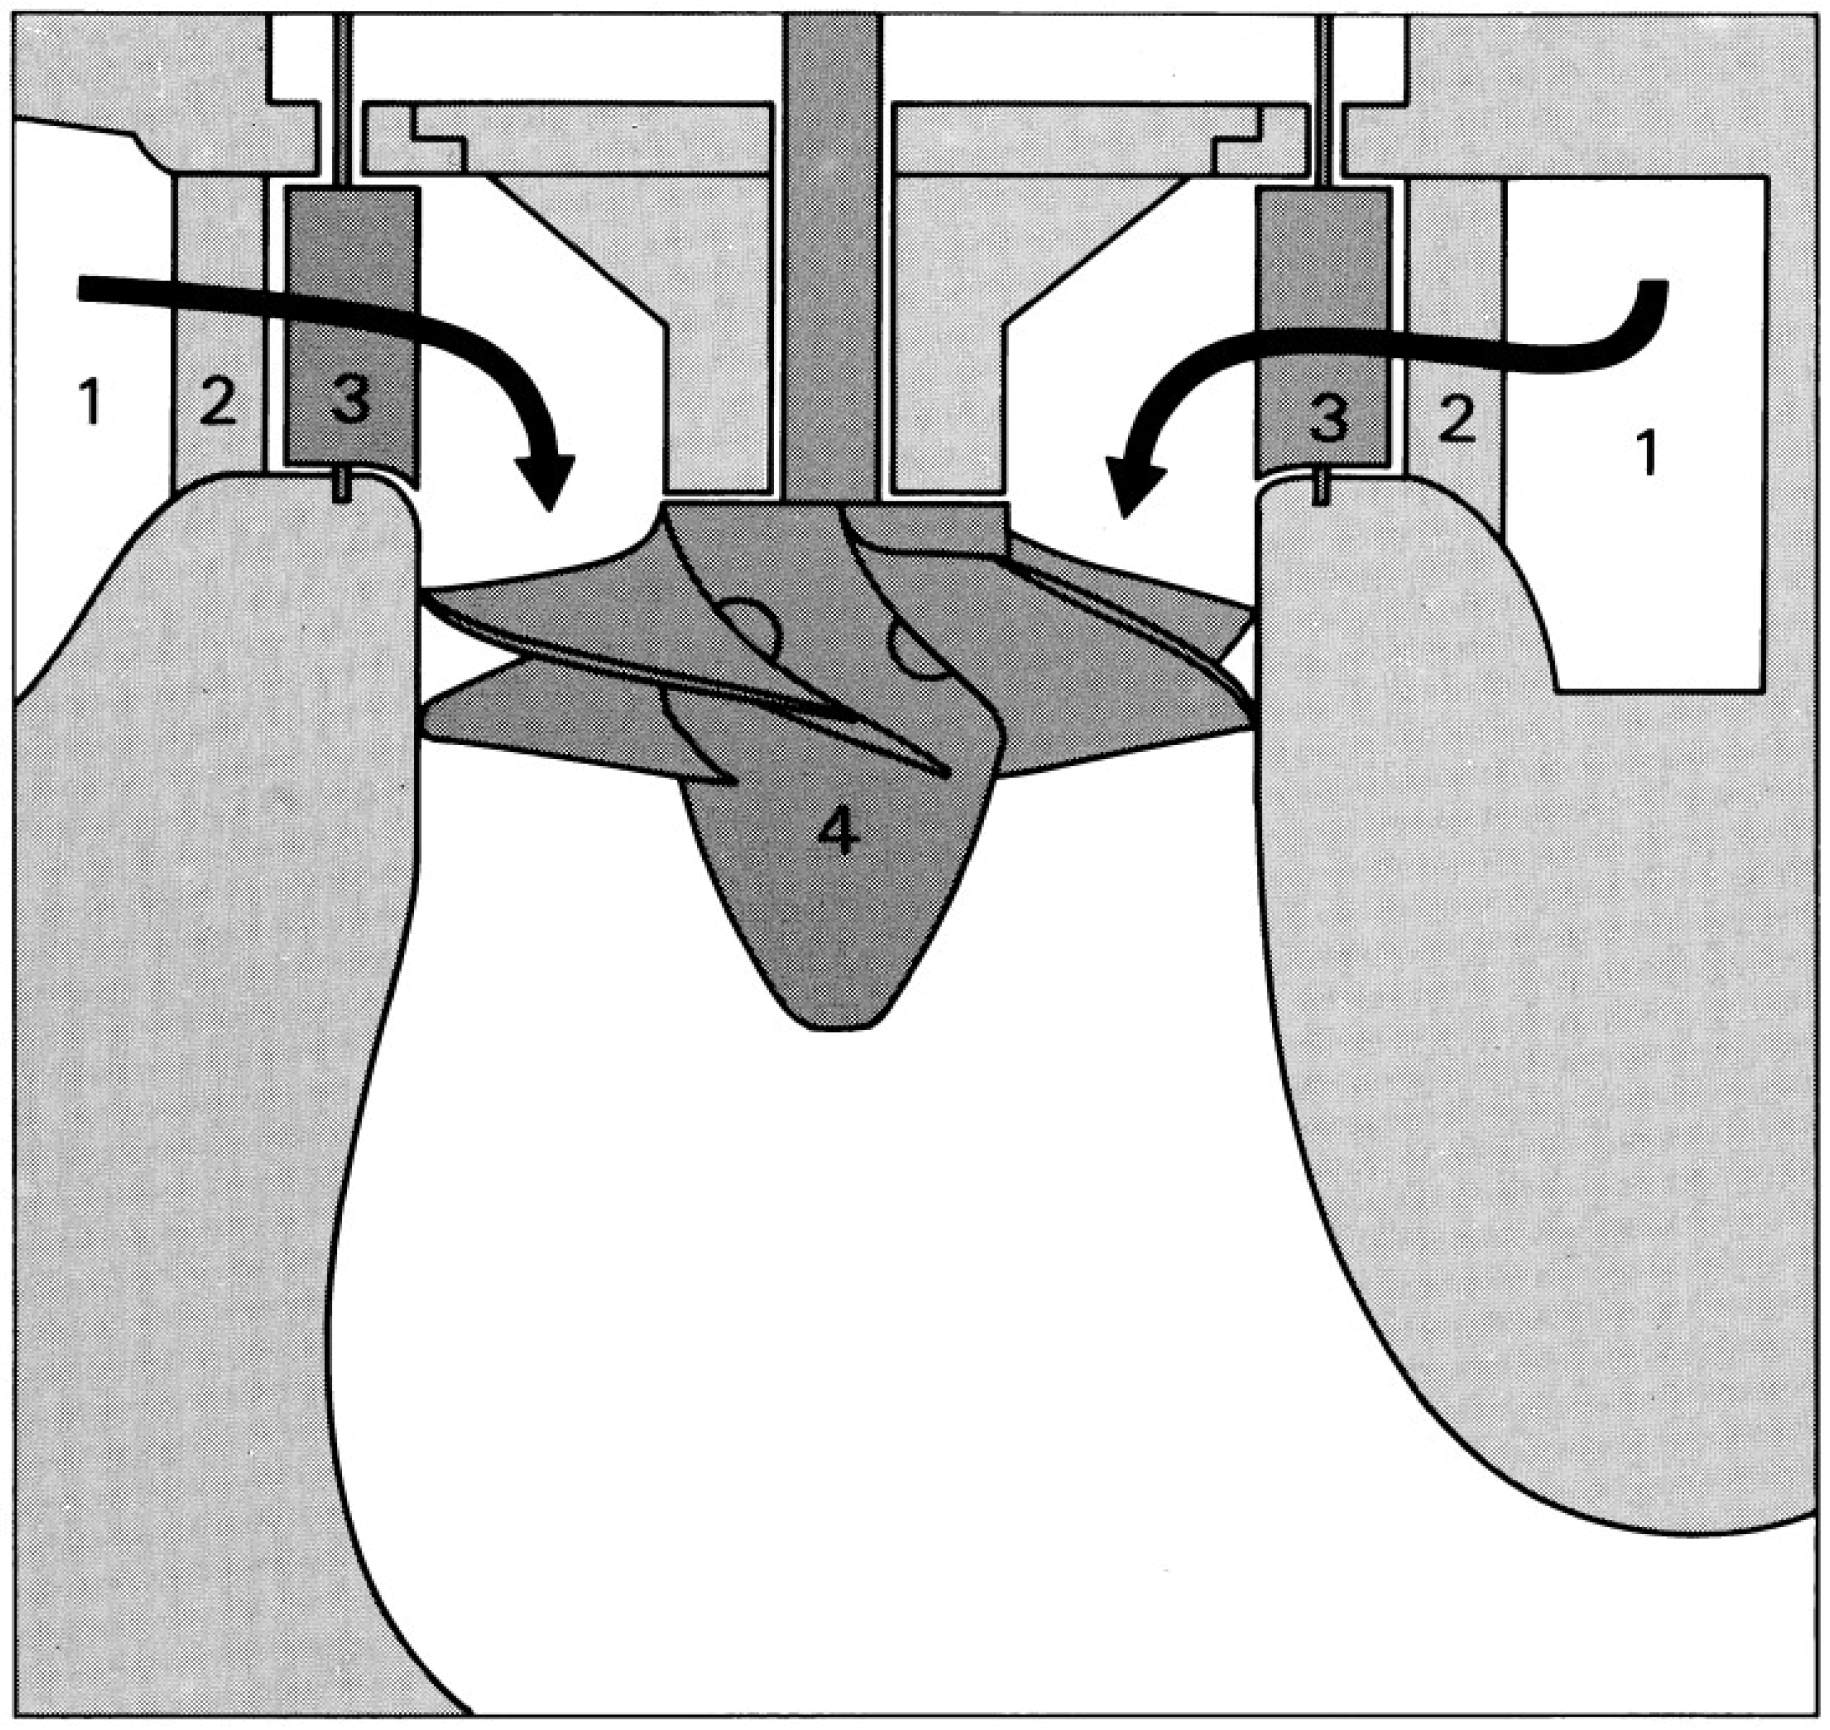
\includegraphics[width=0.85\columnwidth]{images/Kaplan_Turbine.png}    
    \end{minipage}
    \hfill
    \begin{minipage}[t]{0.48\columnwidth}
        \begin{enumerate}
            \item Einlaufspirale
            \item Stützschaufeln
            \item Leitschaufeln
            \item Kaplan-Rad
        \end{enumerate}  
    \end{minipage}

\subsection{Rohrturbinen (horizontale Kaplanturbinen)}
    \begin{minipage}[t]{0.48\columnwidth}
        \centering \vspace{-0.7\baselineskip}
        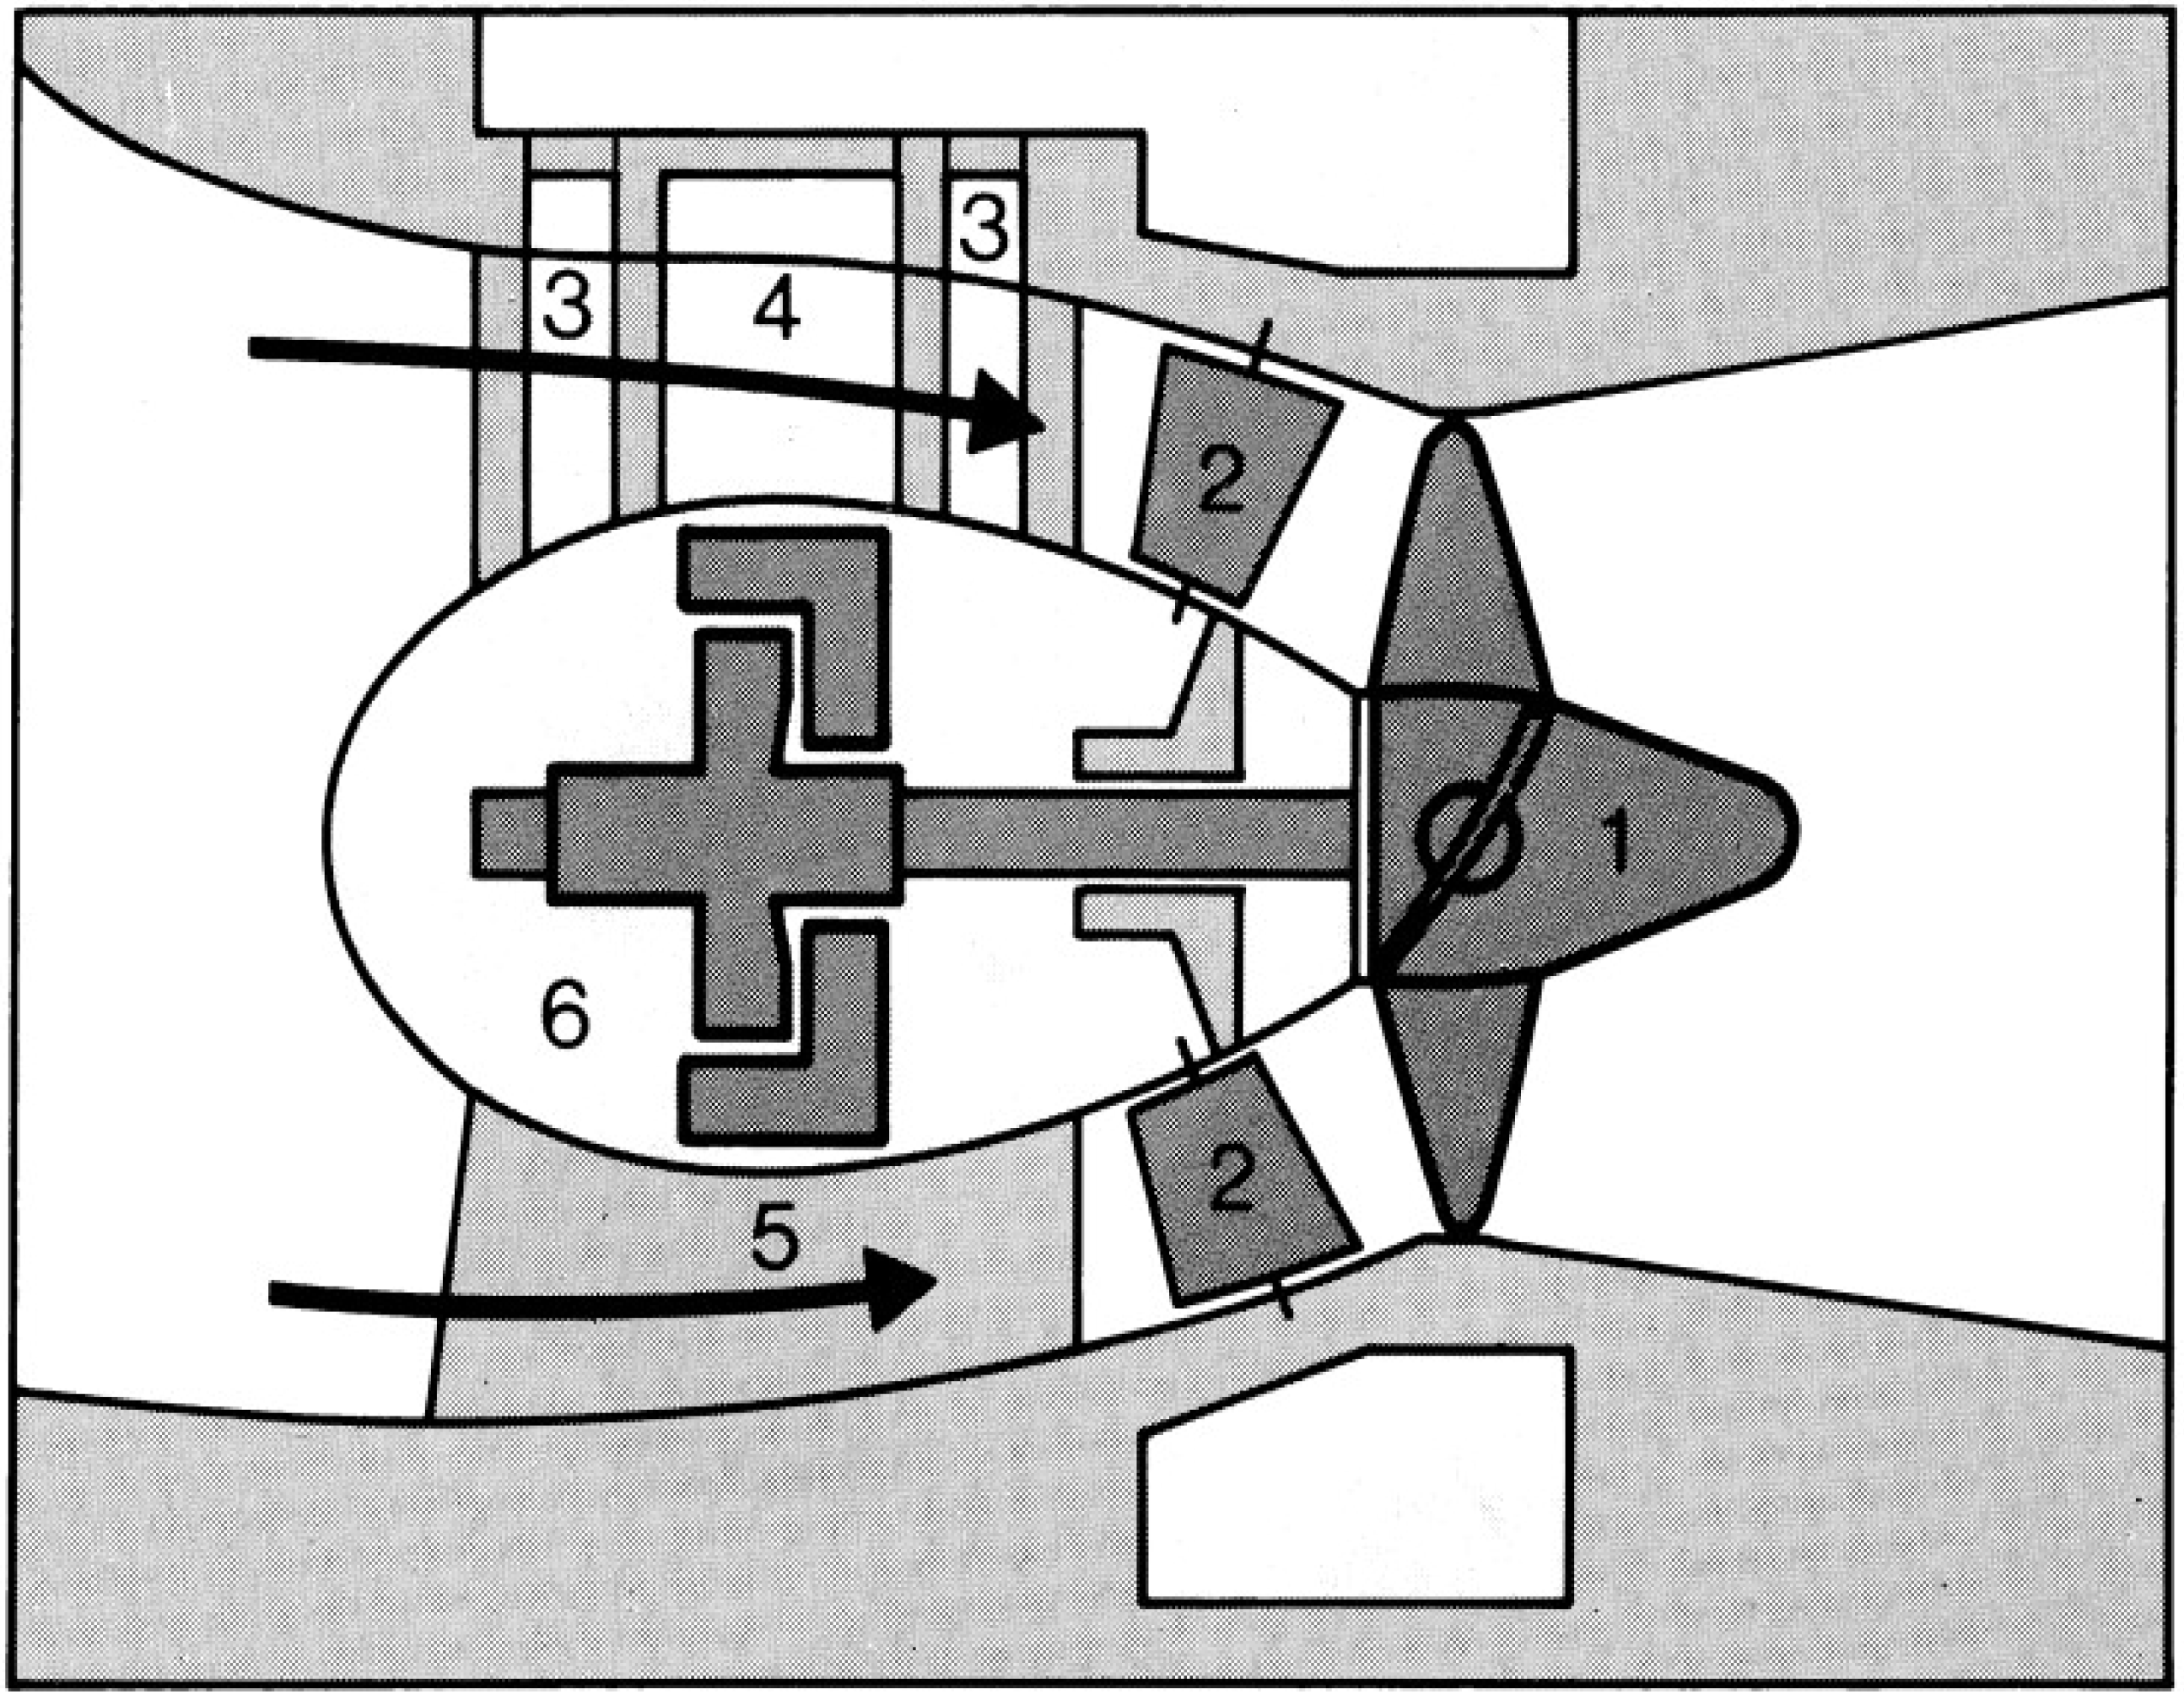
\includegraphics[width=0.85\columnwidth]{images/Rohr_Turbinen.png}    
    \end{minipage}
    \hfill
    \begin{minipage}[t]{0.48\columnwidth}
        \begin{enumerate}
            \item Schaufelrad
            \item Leitschaufeln
            \item Zustiegsschächte
            \item Demontageschacht
            \item Sockel
            \item Generator
        \end{enumerate}  
    \end{minipage}

\subsection{Strafloturbinen}
    \begin{minipage}[t]{0.48\columnwidth}
        \centering \vspace{-0.7\baselineskip}
        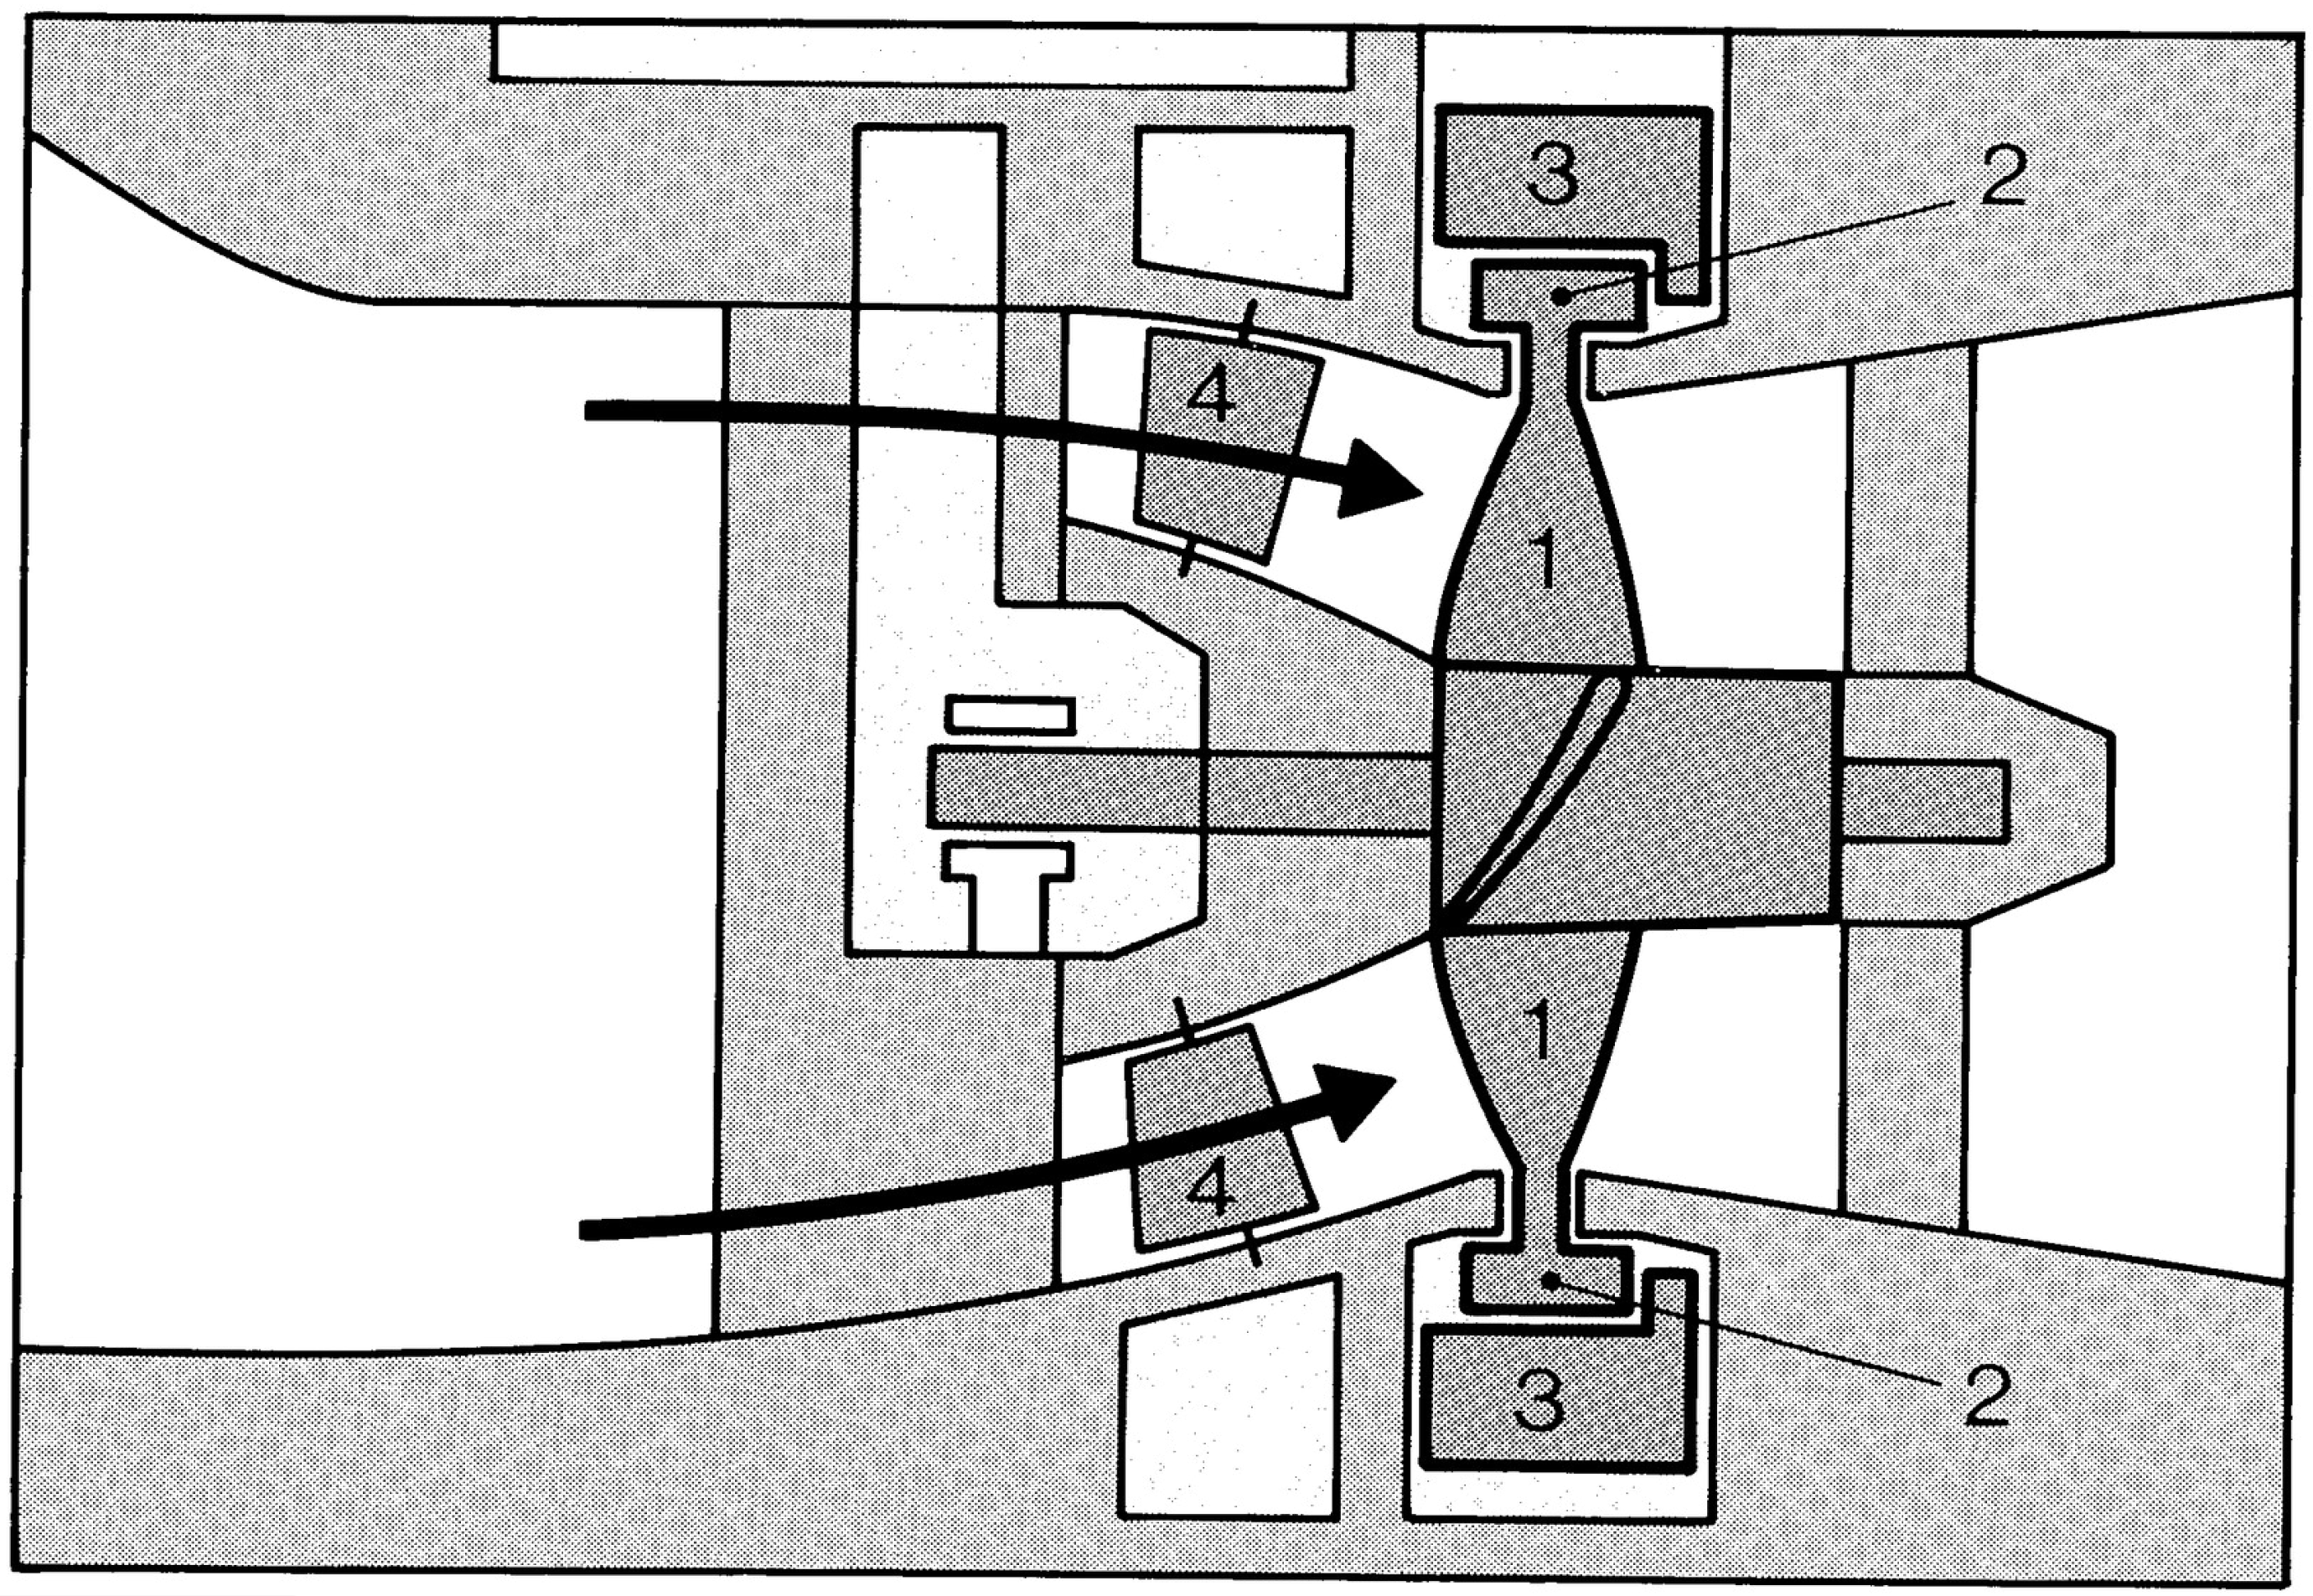
\includegraphics[width=0.85\columnwidth]{images/Straflo_Turbine.png}    
    \end{minipage}
    \hfill
    \begin{minipage}[t]{0.48\columnwidth}
        \begin{enumerate}
            \item Laufradschaufeln
            \item Rotor, Pole des Generators
            \item Stator
            \item Leitschaufeln
        \end{enumerate}  
    \end{minipage}

\subsection{Speicherpumpen und Pumpturbinen}
    \begin{center}
        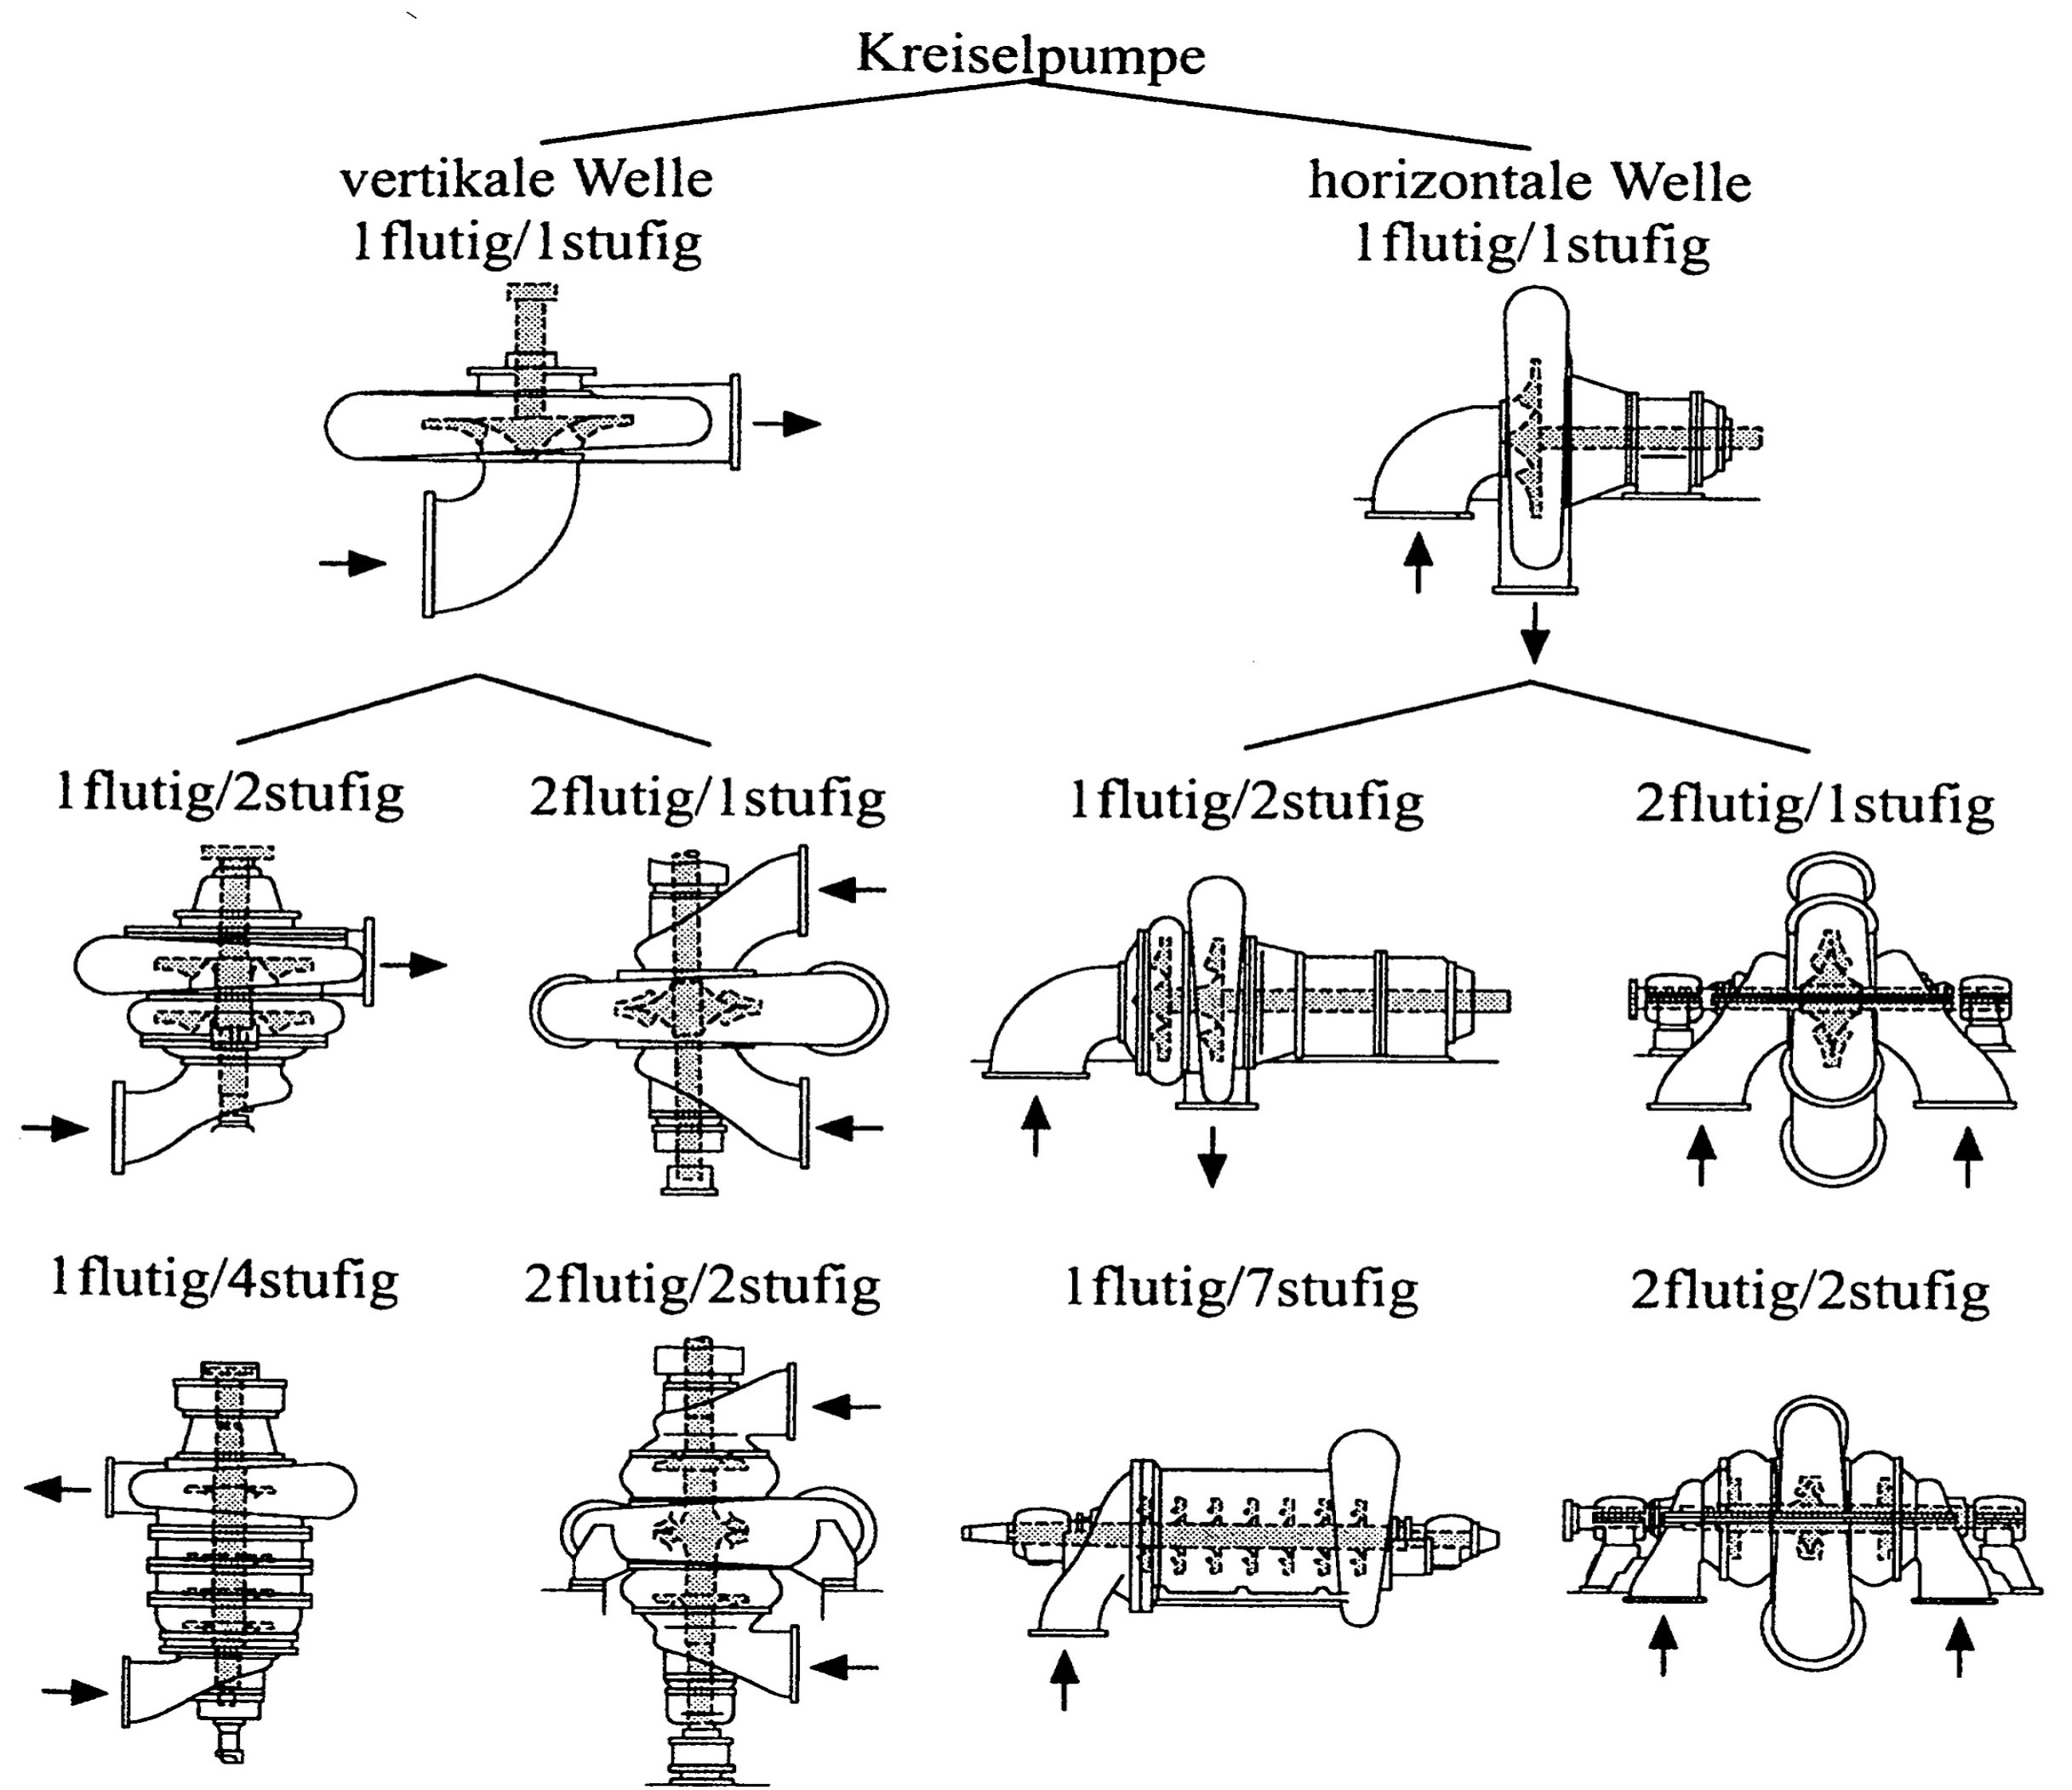
\includegraphics[width=0.9\columnwidth]{images/Speicherpumpen und Pumpturbinen.png}   
    \end{center}

\subsubsection{Dreimaschinensatz}
    Besteht aus: Generator/Motor, Francisturbine und Speicherpumpe

    \vspace{0.1cm}

    \textcolor{red}{\textbf{Nachteile}} 
    \begin{itemize}
        \item Zwei hydraulische Maschinen sowie eine größere Anzahl Abschlussorgane sind nötig.
    \end{itemize}
    \textcolor{green}{\textbf{Vorteil}}
    \begin{itemize}
        \item Unabhängige Optimierung der Turbine und der Pumpe ist möglich.
    \end{itemize}

\subsection{Wahl des Generators}
    Der Generator muss synchron mit dem Netz drehen. Daher muss die definitive Drehzahl der in der Nähe liegenden Synchrondrehzahl entsprechen.

    \vspace{0.15cm}

    \begin{minipage}[t]{0.35\columnwidth}\vspace*{-2mm}
        $\boxed{n = 60 \cdot \frac{f}{p} = \frac{3000}{p}}$
    \end{minipage}%
    \hfill
    \begin{minipage}[t]{0.64\columnwidth}\vspace*{-2mm}
        \renewcommand{\arraystretch}{1.2}
        \begin{tabular}{@{} l p {3.6cm} l @{}}
            $[n]$ & Drehzahl des Generators \dotfill  & $\text{U/min}$ \\
            $[f]$ & Frequenz, meist 50 Hz \dotfill    & $\text{Hz} = \frac{1}{\text{s}}$ \\
            $[p]$ & Polpaarzahl \dotfill              & (1, 2, 3, \dots) \\
        \end{tabular}
    \end{minipage}

\subsection{Kochrezept zur Grob-Auslegung von Pumpen und Turbinen}

\begin{enumerate}
    \item Bestimmung der \textbf{Netto-Fallhöhe} \( H_n \)
    \item Auswahl \textbf{Gesamtdurchfluss} \( Q \), abhängig von Zufluss, Rückhaltemöglichkeit, Einsatztyp (z.B. Spitzenlast)
    \item Bestimmung der \textbf{hydraulischen Leistung} mithilfe der \textbf{elektrischen Leistung} $P_{el} $ und dem Gesamtwirkungsgrad $\eta_{tot}$ :
    \[
    P_\mathrm{hyd} = \rho \cdot Q \cdot g \cdot H_n = \frac{P_{el}}{\eta_{tot}}
    \]
    \item Auswahl \textbf{Turbinentyp}, \textbf{Turbinen-Durchfluss} \( Q \) und \textbf{spezifische Drehzahl} \( n_q \) aus Diagrammen\\
    (ggf. Aufteilung \( Q \) auf mehrere Turbinen / Pumpen)
    \item Bestimmung der \textbf{Turbinen-Drehzahl}:
    \[
    n = n_q \cdot \frac{H_n^{3/4}}{Q^{1/2}}
    \]
    \item Bestimmung der \textbf{Polpaarzahl}:
    \[
    p = \frac{3000}{n}
    \]
    (auf ganze Zahl runden und prüfen, ob \( n_q \) nach Rundung noch im möglichen Bereich liegt)
    \item Weitere Bedingungen zur \textbf{Feinauslegung}:
    \begin{itemize}
        \item Teillastverhalten, Wirkungsgrad, Betriebsbereiche
        \item Räumliche Bedingungen, Simulationen, Experimente
        \item \(\ldots\)
        \item Lösung ist ein Abwägen und iterativer Prozess
    \end{itemize}
\end{enumerate}
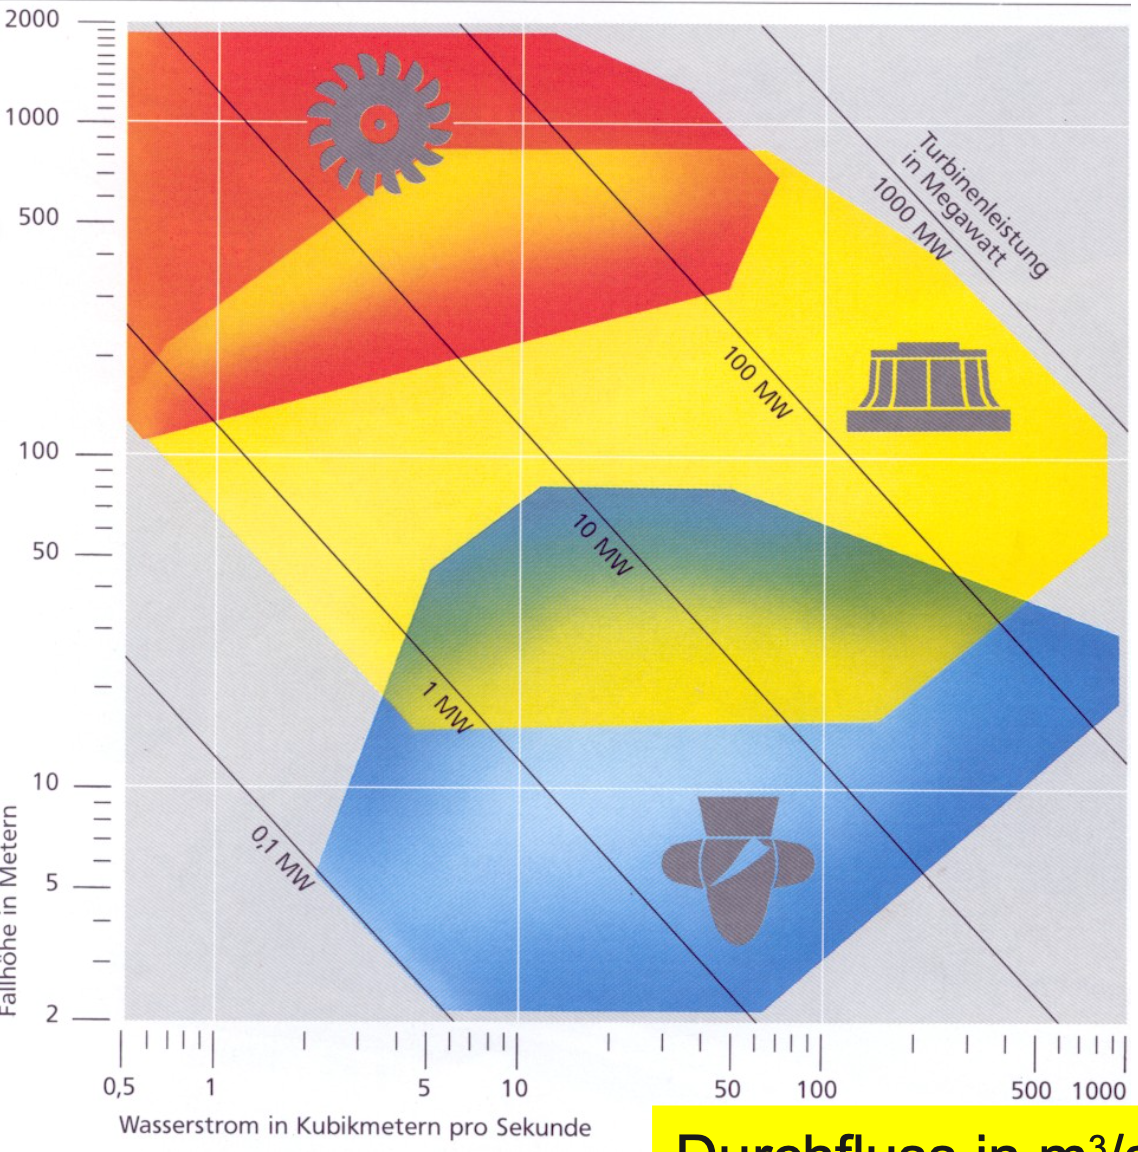
\includegraphics[width=1\linewidth]{images/Turbinentypen.png}
\textcolor{red}{Peltonturbine}, \textcolor{yellow}{Francisturbine}, \textcolor{blue}{Kaplanturbine}

\newcolumn
 % done
        \section{Thermische Kraftwerke/ Dampfkraftwerke}
    Gegen 90\% der weltweiten Bereitstellung
    elektrischer Energie erfolgt in «Thermischen Kraftwerken».\\
    Kraftwerksarten:
    \begin{itemize}
        \item Thermische Kraftwerke auf fossiler Basis
    (Dampf-, Gasturbinen-, Gas- und Dampfturbinen-Kraftwerke (GUD), Blockheiz-, Diesel- Kraftwerke)
        \item Kernkraftwerke
        \item Geothermische Anlagen
        \item Solarthermische Anlagen
        \item Heizkraftwerke
        \item Kehrichtverbrennung mit thermischem Kraftwerk
    \end{itemize}

\subsection{Funktionsweise}
    \begin{center}
        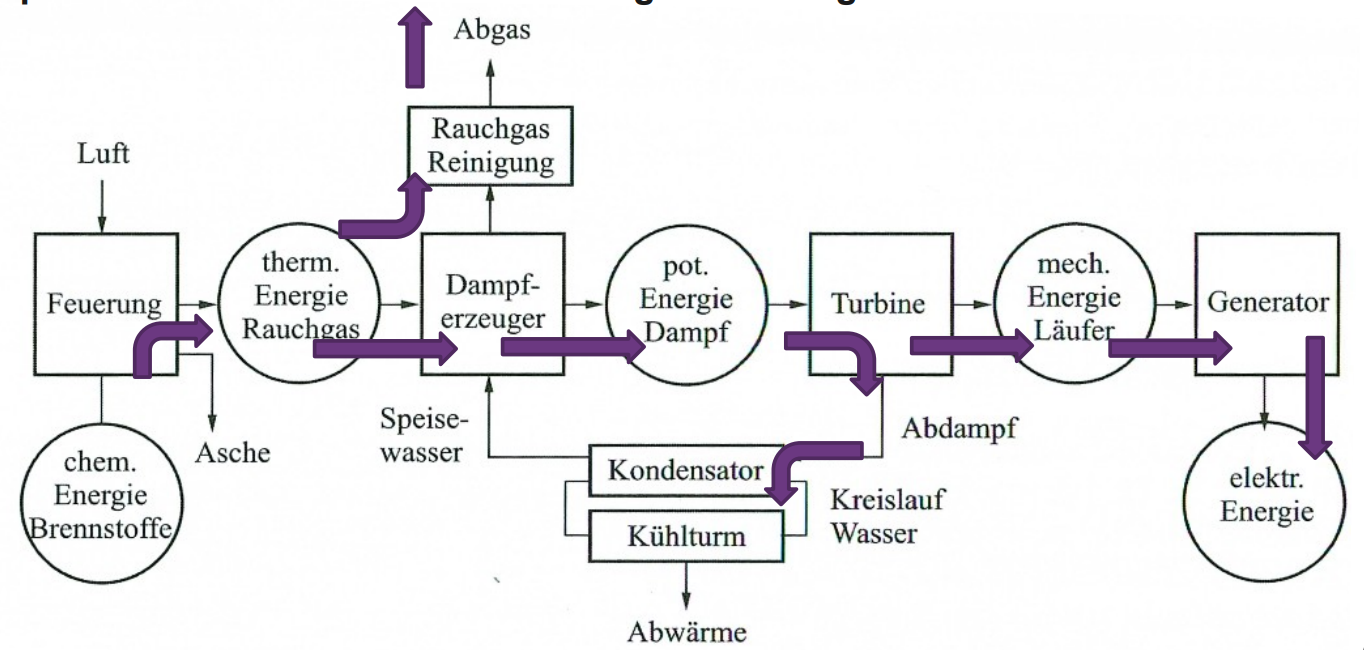
\includegraphics[width=0.9\columnwidth]{images/Prinzip_Thermisch.png}\\
    \end{center}

    \begin{minipage}[t]{0.49\columnwidth}
        \centering \vspace{-0.7\baselineskip}
        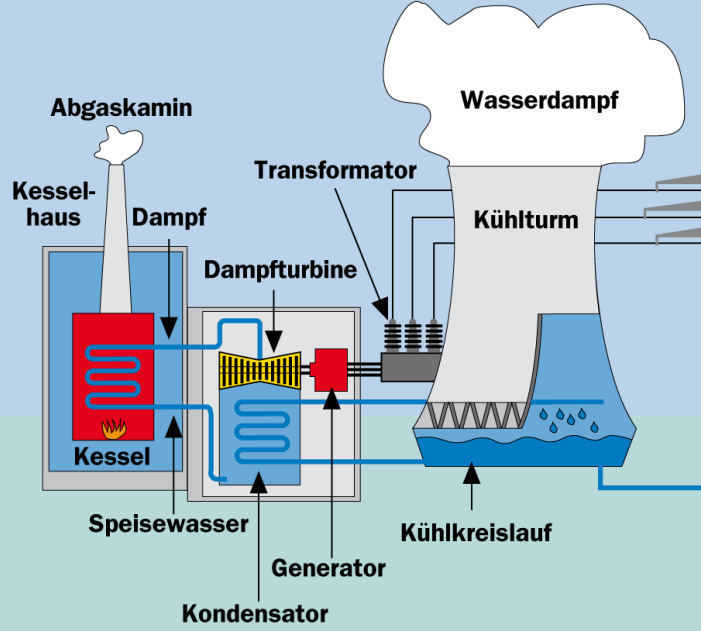
\includegraphics[width=0.85\linewidth]{images/Prinzip2_Thermisch.png}
    \end{minipage}%
    \hfill
    \begin{minipage}[t]{0.49\columnwidth}
        \begin{enumerate}
            \item Brenn- und Treibstoffe, Geothermie, Solarthermie, atomare Bindungsenergie
            \item Thermische Energie in Form von Gas oder Dampf
            \item Gas- oder Dampfturbine
            \item Generator
            \item Transformator/Netz
        \end{enumerate}
    \end{minipage}

\subsection{Thermodynamik}
    \begin{center}
        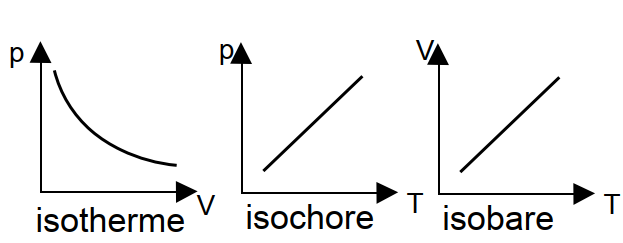
\includegraphics[width=0.9\linewidth]{images/Thermo.png}
    \end{center}

    \begin{tabular}{@{}l l}
        \textbf{isotherme:}     & $T = \text{const}\quad W = m \cdot Ri \cdot T \cdot \mathrm{ln}\left(\frac{p2}{p1} \right)$\\
        \textbf{isochore:}      & $V = \text{const}\quad Q = c_v \cdot m \cdot \Delta T$\\
        \textbf{isobare:}       & $p = \text{const}\quad Q = c_p \cdot m \cdot \Delta T$\\
        \textbf{isotrop:}       & Entropie bleibt konstant $ \frac{T1}{T2} = \left( \frac{p_1}{p_2}\right) ^{\frac{x-1}{x}}= \frac{T_4}{T_3}$\\
        \textbf{adiabatisch:}   & Zustandsänderung ohne Wärmetausch mit der Umgebung\\
        \textbf{ideales Gas:}   & $\frac{p\cdot v}{T} = \text{const}$\\
        \textbf{Enthalpie:}     & Wärmeinhalt, $H=U+p\cdot V$, $U$: innere Energie\\
        \textbf{Entropie:}      & Energie pro Temperatur $T$, Entropieänderung $\Delta S =\frac{Q}{T}$, $Q$: zugef. Wärme \\
    \end{tabular}

\subsection{Kreisprozesse}
\subsubsection{Carnot Prozess}
    Wärme (Dampferzeuger) -> Mechanische Arbeit (Dampfturbine)

    \begin{minipage}[ht]{0.49\columnwidth}
        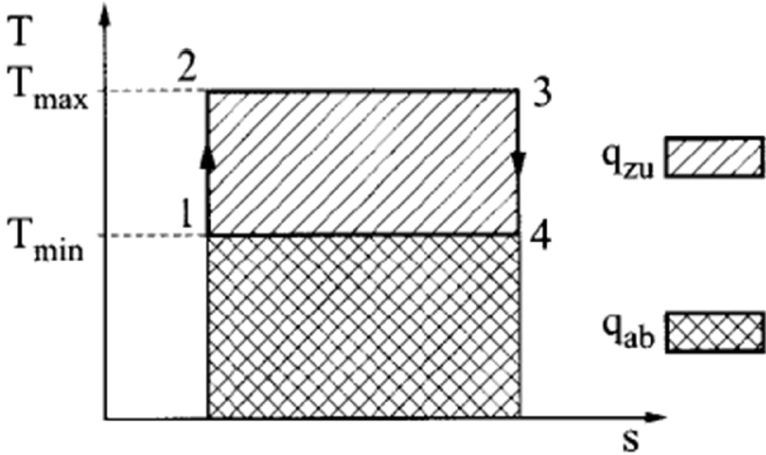
\includegraphics[width=0.95\linewidth]{images/carnot1.png}
    \end{minipage}
    \begin{minipage}[ht]{0.49\columnwidth}
        \textbf{Carnot-Prozess im T, s - Diagramm}\\
        Nutzbare Arbeit: $w_nutz = q_{zu} - q_{ab}$\\Da die Entropie als $dq = T \cdot ds$ definiert ist, erscheint sowohl die dem Prozess zugeführte Wärme $q_{zu} = T_{max} ( s_3 - s_2 )$ als auch die abgeführte Wärme $q_{ab} = T_{min} (s_4 - s_1)$  als Fläche im T, s -Diagramm.\\
        Der Wirkungsgrad des Carnot-Prozesses ergibt sich somit:
    \end{minipage}

    \textbf{Thermischer Wirkungsgrad}

    $\boxed{\eta_{\mathrm{th}}' 
    = \frac{P_m - P_u}{P_{zu}}
    = \frac{(h_3 - h_{4^*}) - (h_{2^*} - h_1)}{(h_3 - h_{2^*})}
    = 1 - \frac{P_{ab}}{P_{zu}}
    = 1 - \frac{(h_{4^*} - h_1)}{(h_3 - h_{2^*})}
    = 1 - \frac{h_{4^*} - h_1}{h_3 - h_{2^*}}}$

    \begin{tabular}{@{} l p{7.5cm} l @{}}
    $[P_m]$ & abgegebene mechanische Leistung der Wärmekraftmaschine \dotfill & $\mathrm{kW}$    \\
    $[P_{u}]$ & Leistung der (elektrisch angetriebenen) Speisewasserpumpe \dotfill & $\mathrm{kW}$    \\
    $[P_{zu}]$ & Leistungszufuhr aus dem Kessel \dotfill & $\mathrm{kW}$    \\
    $[P_{ab}]$ & abzuführende Wärmeleistung im Kondensator \dotfill & $\mathrm{kW}$    \\
    $[h]$ & spezifische Enthalpie \dotfill & $\mathrm{kJ/kg}$ \\
    $[Q]$ & Wärmemenge \dotfill & $\mathrm{J}$ \\
    \end{tabular}

\subsubsection{Wirkungsgrad erhöhen}
    \vspace{-4mm}
    \def\columnseprulecolor{\color{white}}
    \begin{multicols}{2}
        \begin{itemize}  
            \item Zwischenüberhitzung
            \item Speisewasservorwärmung
            \item Erhöhung des Dampfdrucks und der Temperatur
            \item Kombination mit Gasturbine (GuD-Prozess)
        \end{itemize}
    \end{multicols}
    \def\columnseprulecolor{\color{black}}

\subsection{Joule-Prozess für Gasturbinen}
\begin{minipage}[ht]{0.49\columnwidth}
    \centering \vspace{-0.7\baselineskip}
    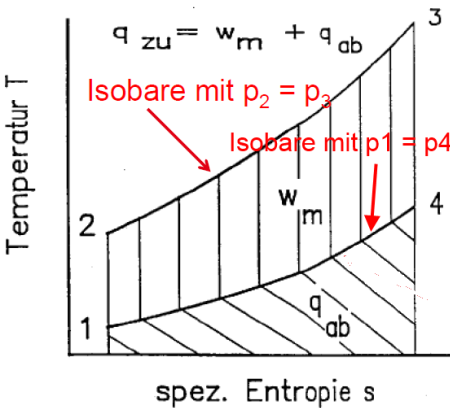
\includegraphics[width=0.85\linewidth]{images/carnot2.png}
\end{minipage}
\begin{minipage}[ht]{0.49\columnwidth}
    \textbf{Joule-Prozess im T, s - Diagramm}

    \textbf{Ablauf:}
    \begin{itemize}
        \item[1-2] Verdichtung, $s$ const, $p$ steigt (isotrop)
        \item[2-3] Erwärmung, $s$ steigt, $T$ steigt, $p$ konstant (isobar)
        \item[3-4] Entspannung, $s$ konstant, $p$ sinkt (isotrop)
        \item[4-1] Abkühlung, $s$ sinkt, $T$ sinkt, $p$ konstant (isobar)
    \end{itemize}
\end{minipage}

\subsection{Enthalpie}
    \begin{minipage}[ht]{0.49\columnwidth}
        \centering \vspace{-0.7\baselineskip}
        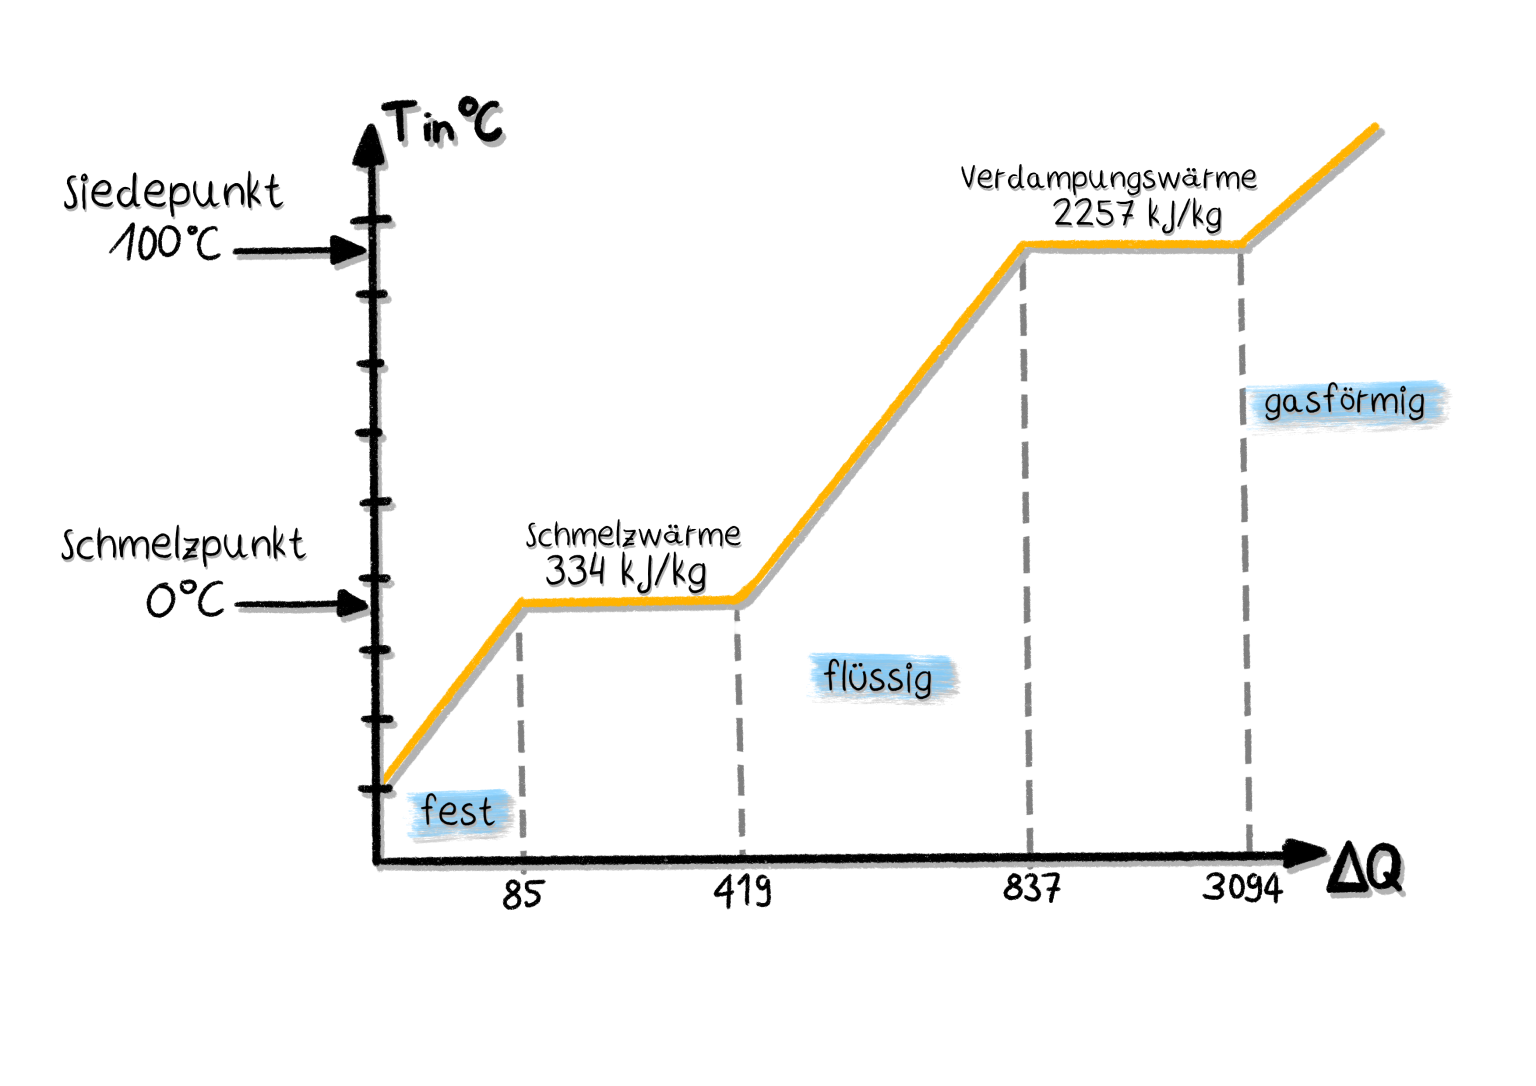
\includegraphics[width=0.85\columnwidth]{images/Wasserverlauf.png}

    \end{minipage}
    \begin{minipage}[ht]{0.49\columnwidth}
        $\boxed{dH= dQ + V\cdot dp}$ d.h. Enthalpie ändert mit Druck

        Verdampfungswärme: $\boxed{q_V=T_V\cdot \Delta S}$

        \textbf{Arregatsänderungen:}

        Fest - Flüssig: Schmelzen/ erstarren

        Flüssig - Gas: Verdampfen/ kondensieren

        Fest - Gas: Sublimieren/ Resublimieren

        $0^\circ$C = 273K
    \end{minipage}

\subsection{Mollier-Diagramm}
    \begin{center}
        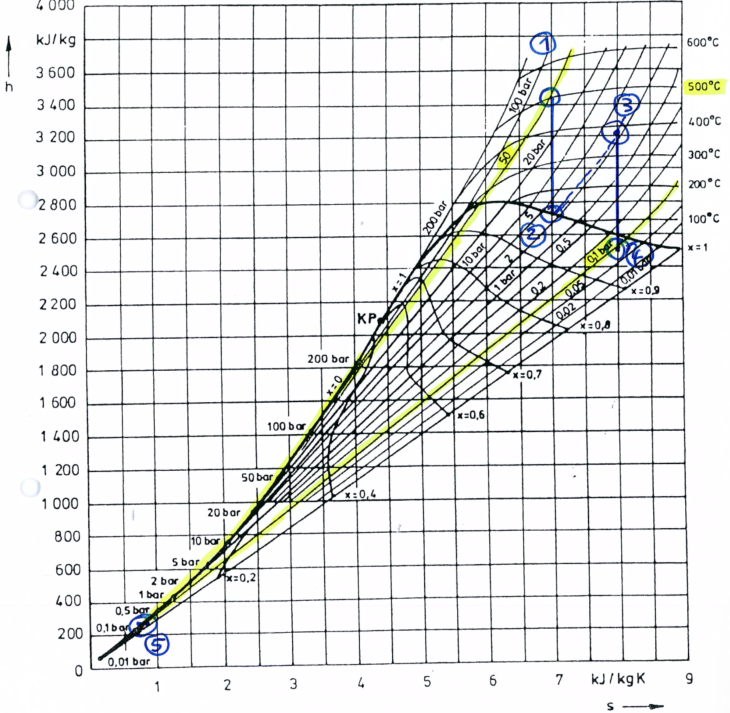
\includegraphics[width=0.85\columnwidth]{images/hsDiagramm.png}\\
    \end{center}

    Dampfturbine mit Zwischenüberhitzung

    \begin{tabular}{@{}l l}
        \circled{1}                & Startdruck: $500\, \mathrm{^\circ C}$ $50\, \mathrm{bar}$ \\
        \circled{1} zu \circled{2} & Entspannung in Turbine \\
        \circled{2} zu \circled{3} & Temperaturzuf. mit konst. Druck (isobar), Dampferzeuger(Energieeintrag,Q) \\
        \circled{3} zu \circled{4} & Entspannung in Turbine \\
    \end{tabular}

    $\boxed{x=\frac{m_D}{m_W + m_D}}$
    $\boxed{\frac{m_w}{m_d}= \frac{1}{x}-1}$
    $\boxed{\Delta h_{liquid}= V \cdot \Delta p}$
    $(1  Bar = 10^5pa)$

    $\boxed{P = \dot{m}_D \cdot \Delta h}$
    $\boxed{P_{\text{mech}} = \dot{m}_k \cdot \eta_{\text{Th}} \cdot \eta_{\text{DE}} \cdot H}$
    $\boxed{\eta_{\mathrm{th}}
    = 1 - \frac{P_{ab}}{P_{zu}}
    = 1 - \frac{\Sigma h_{tief}}{{\Sigma h_{hoch}}}} $
    $\boxed{\eta_\mathrm{c} = 1-\frac{T_U}{T_O}}$

    \crd{Senkrechte $[\Delta h]$ nicht beachten bei der Berechnung von Wirkungsgrad des Kreisprozesses.}

    \begin{tabular}{@{} l p{7.5cm} l @{}}
    $[x]$ & Wasserdampfgehalt \dotfill &    \\
    $[m_D]$ & Dampfmassegehalt \dotfill & $\mathrm{kg/m^3}$    \\
    $[m_W]$ & Wassermassegehalt \dotfill & $\mathrm{kg/m^3}$    \\
    $[\Delta h]$ & Entropie zweier Punkte senkrecht verbunden \dotfill & $\mathrm{kJ/\ kg}$   \\
    $[V]$ & Volumen $0.001\,\mathrm{\frac{m^3}{kg}}$\dotfill & $\mathrm{m^3}$ \\
    $[\Delta p]$ & Druckunterschied \dotfill & Pa \\
    $[\eta_{\mathrm{th}}]$ & Thermischer Wirkungsgrad \dotfill &  \\
    $[\eta_{\mathrm{c}}]$ & Carnot-Faktor \dotfill &  \\
    $[T_o]$ & Höchste Temperatur Prozess \dotfill & $\mathrm{K}$ \\
    $[T_u]$ & Tiefste Temperatur über x=1 Grenze \dotfill & $\mathrm{K}$ \\
    $[P_{\text{mech}}]$ & Mechanisch abgegebene Leistung \dotfill & $\mathrm{W}$ \\
    $[\dot{m}_k]$ & Massenstrom des eingesetzten Brennstoffs \dotfill & $\mathrm{kg/s}$ \\
    $[\eta_{\text{th}}]$ & Thermischer Wirkungsgrad \dotfill &  \\
    $[\eta_{\text{DE}}]$ & Wirkungsgrad der Dampferzeugung bzw. Energieumwandlung \dotfill &  \\
    $[H]$ & Heizwert des Brennstoffs \dotfill & $\mathrm{J/kg}$ \\
    \end{tabular}


\subsection{Anleitung Mollier Diagramm (s - h)}
\subsubsection{Clausius-Rankine-Prozess}
    Sattdampfprozess (Dampfkreislauf)

    1 - 2 Druckerhöhung mit Speiseerhöhung (von 1 Bar bis Zieldruck, senkrecht links unten)

    \textcolor{ForestGreen}{2 - 3 Dampferzeuger, Energiezugabe (Druck bleibt konstant)}

    \textcolor{purple}{3 - 4 Dampfturbine, Energieumwandlung zu mechanisch (Druckabnahme, s bleibt konstant (senkrechte Linie))}

    \textcolor{red}{4 - 1 Kondensator, zurück zum Start, Verlustenergie (Druck konstant)}

    \begin{center}
        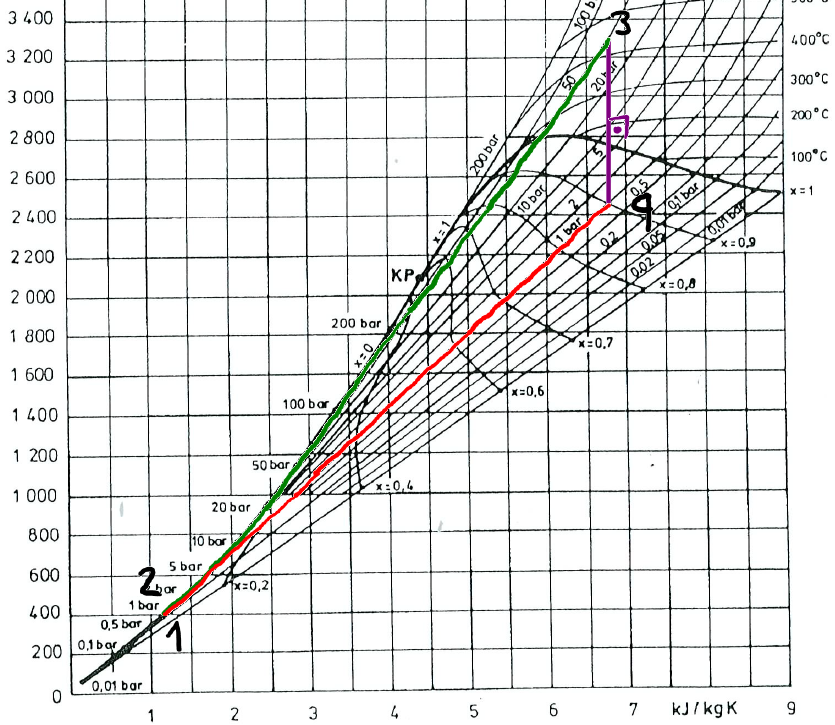
\includegraphics[width=0.9\columnwidth]{images/Sattdampf.png}
    \end{center}

    \begin{center}
        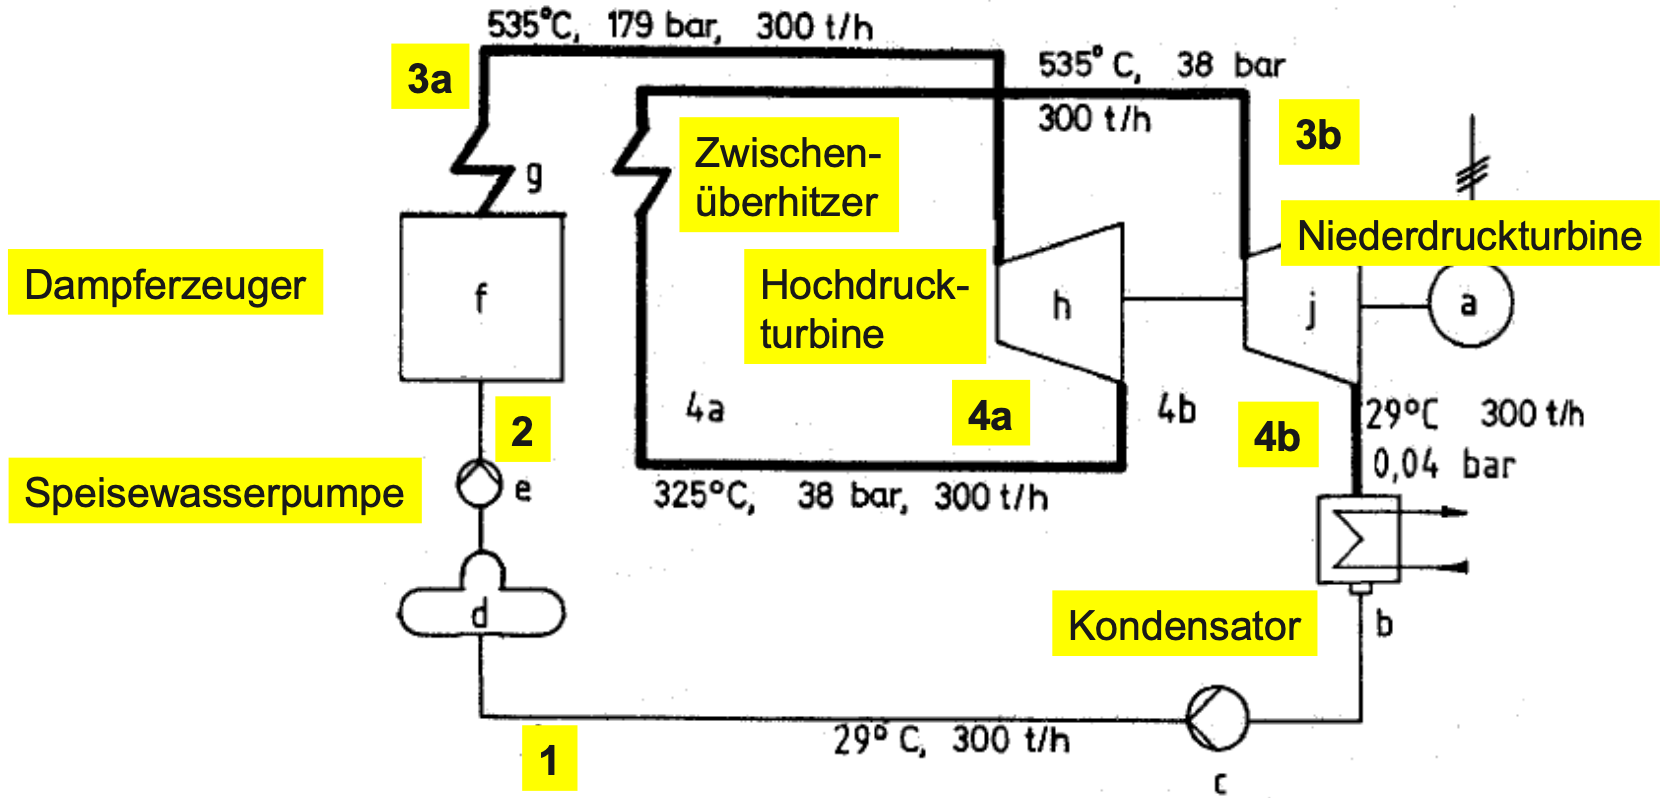
\includegraphics[width=0.9\columnwidth]{images/DampfkraftMitZwischenueberhitzung.png}
    \end{center}

    Wirkungsgrad:

    \begin{minipage}[c]{0.4\columnwidth}
        $\boxed{\eta_{\mathrm{th}} = 1-\frac{h_{\mathrm{4b}}-h_{\mathrm{1}}}{(h_{\mathrm{3a}}-h_{\mathrm{2}})+(h_{\mathrm{3b}}-h_{\mathrm{4a}})}}$
    \end{minipage}
    \hfill
    \begin{minipage}[c]{0.6\columnwidth}
        \centering \vspace{-0.7\baselineskip}
        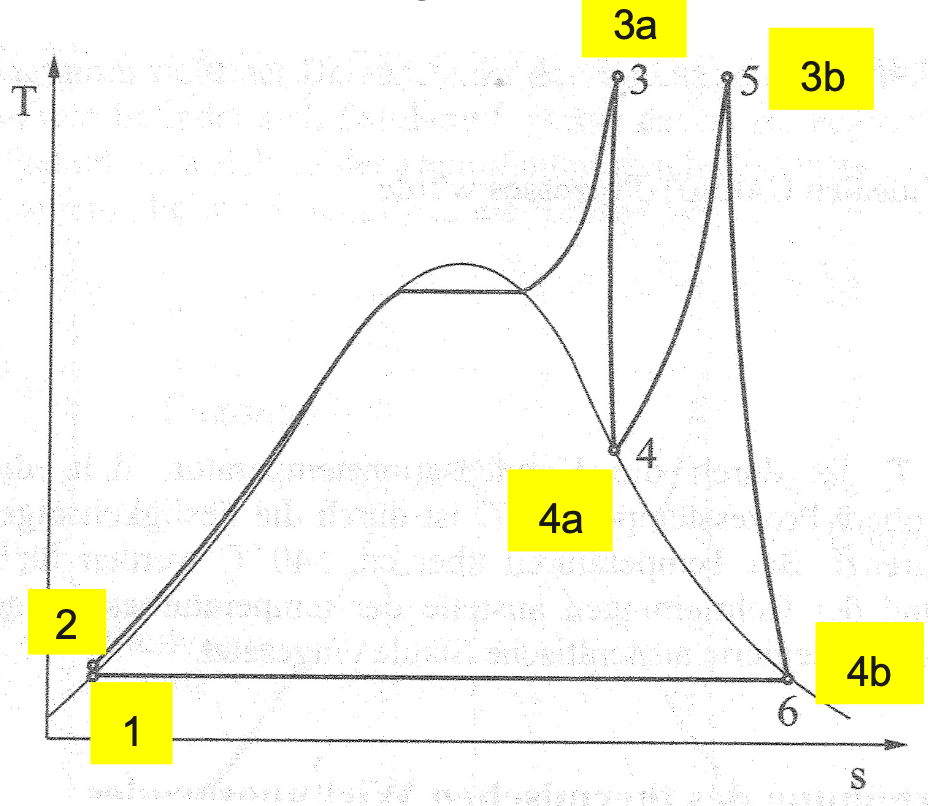
\includegraphics[width=0.8\linewidth]{images/Zwischenueberhitzung.png}
    \end{minipage}

\subsection{Varianten}
    Dampfkraftwerk mit Zwischenüberhitzung oder mit Abwärmenutzung

\subsection{Komponenten}
    \begin{minipage}[t]{0.49\columnwidth}
        Komponenten fossil befeuerten Dampfkraftwerke
        \begin{itemize}
            \item Kessel und Dampferzeuger
            \item Rauchgasreinigung
            \item Feuerungen und Brenner
            \item Dampferzeuger mit Wirbelschichtfeuerung
            \item Dampfturbinen
            \item Kühlsysteme für Dampfkraftwerke
        \end{itemize}
    \end{minipage}%
    \hfill
    \begin{minipage}[t]{0.49\columnwidth}
        \textbf{Kühlsysteme:}

        \begin{itemize}
            \item Frischwasserkühlung
            \item Ablaufkühlung
            \item Nasse Rückkühlung
            \item Trockene Rückkühlung
            \begin{itemize}
                \item direktes System
                \item indirekt mit Mischkondensator
                \item indirekt mit Oberflächenkondensator
            \end{itemize}
        \end{itemize}
    \end{minipage}

    \begin{minipage}[ht]{0.49\columnwidth}
        \textbf{Kohlestaubbrenner:}

        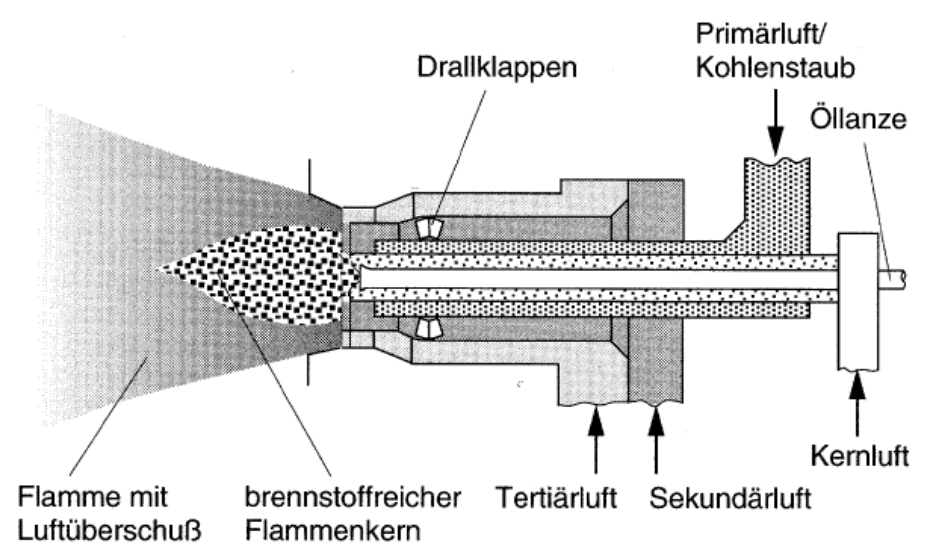
\includegraphics[width=0.9\columnwidth]{images/Kohlestaub.png}\\
    \end{minipage}
    \hfill
    \begin{minipage}[ht]{0.49\columnwidth}
        \textbf{Gasreinigung:}

        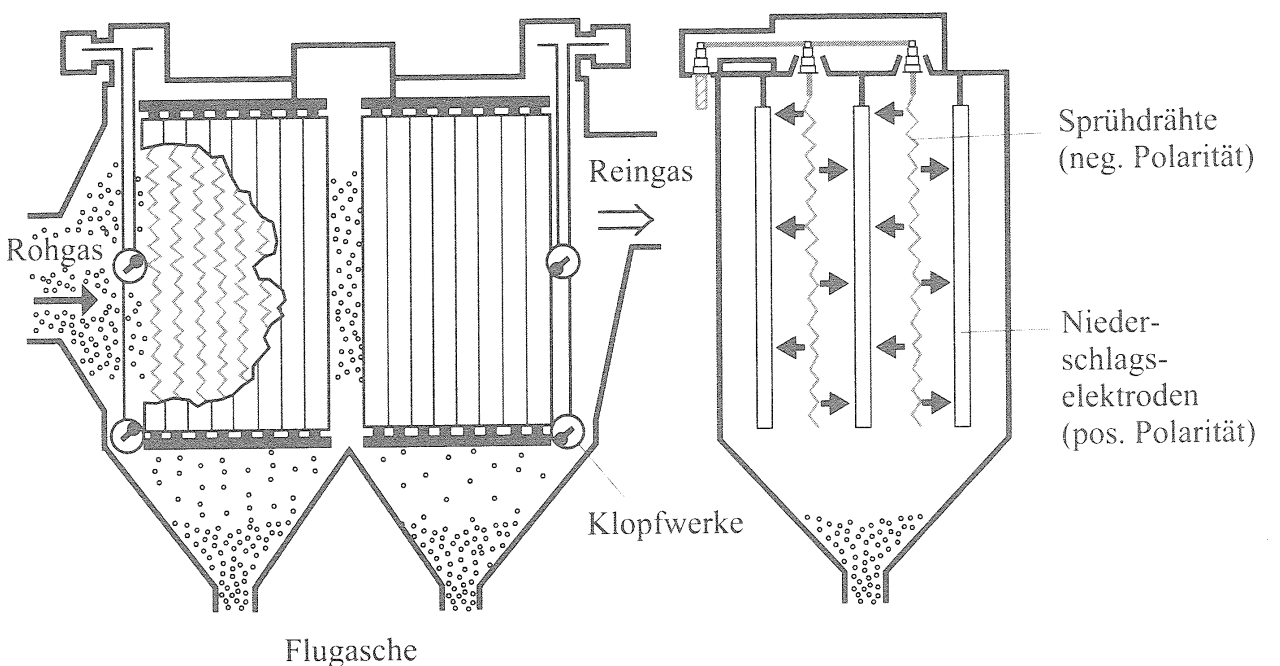
\includegraphics[width=0.9\columnwidth]{images/GAsreinigung.png}\\
    \end{minipage}

    \begin{center}
        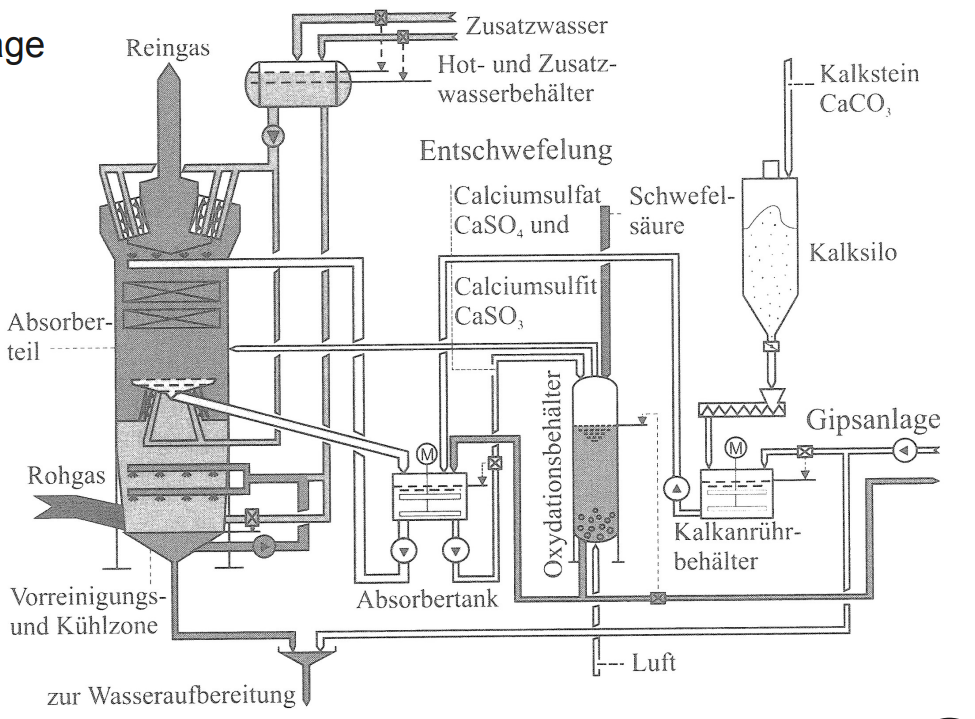
\includegraphics[width=0.9\columnwidth]{images/Entschwefelung.png}\\
    \end{center}

\begin{minipage}[ht]{0.49\columnwidth}
    \textbf{Turbine:}

    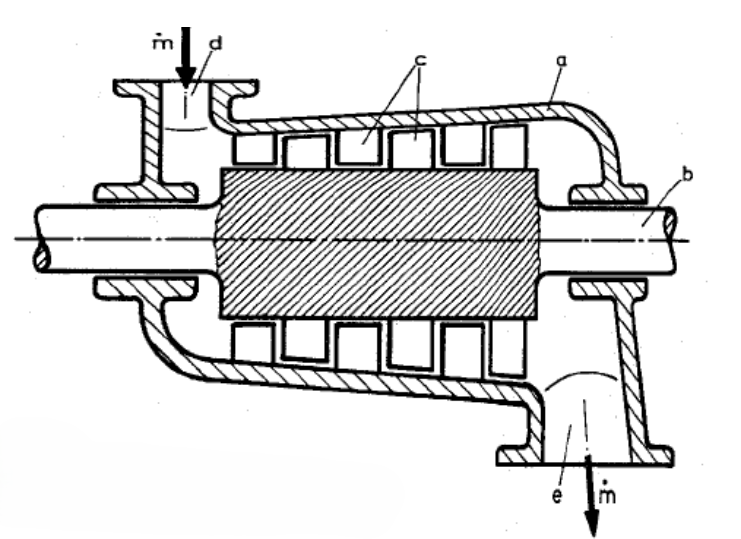
\includegraphics[width=0.9\columnwidth]{images/dampfturbine.png}
\end{minipage}
\hfill
\begin{minipage}[ht]{0.49\columnwidth}
    \begin{itemize}
        \item[a] Gehäuse 
        \item[b] Läufer 
        \item[c] Schaufeln 
        \item[d] Einströmstützen 
        \item[e] Ausstromstutzen 
        \item[f] Zylinderschnitt
        \item[g] Leitgitte
        \item[h] Lauftgitte
        \item[m] Massestrom mediu
        \item[$F_\tau$] Tangetialkraft Laufrad 
    \end{itemize}
\end{minipage} % done
        \section{Atomkraftwerk}
\subsection{Merkmale Nukleare Dampferzeugung}
    \begin{outline}
        \1 Leistungsfähige Energiequelle
        \1 CO2 - freie Produktion elektrischer Energie
        \1 Aufwändige Technologie
        \1 Sicherheit
        \1 Tiefenlager radioaktiver Stoffe
        \1 Diskussion in Politik, Gesellschaft, Ethik
    \end{outline}

\subsubsection{Kernprozesse für die Energiegewinnung}
    \begin{outline}
        \1 Künstliche Kernspaltung schwerer Kerne (Fission)
            \2 → Kernkraftwerke 3. Generation
            \2 (Stand der Technik)
        \1 Umwandlung von schweren Kernen in gut spaltbare Kerne im Brutprozess (Konversion)
            \2 → Kernkraftwerke 4. Generation
            \2 (in Entwicklung)
        \1 Verschmelzung leichter Kerne zu einem Kern (Fusion)
            \2 → Grundlagenforschung in Bearbeitung
    \end{outline}


\subsection{Kernphysikalische Grundlagen}
    \begin{minipage}[t]{0.39\columnwidth}\vspace*{-2mm}
        $\boxed{A = Z + N}$ 

        Nuklid-Schreibweise: $\boxed{\text{\ce{^{A}_{Z}Element}} }$ 

        \text{z.\,B.} \quad \text{\ce{^{235}_{92}U}}
    \end{minipage}%
    \hfill
    \begin{minipage}[t]{0.6\columnwidth}\vspace*{-2mm}
        \renewcommand{\arraystretch}{1.2}
        \begin{tabular}{@{} l p {4.2cm} l @{}}
            $[A]$ & Anzahl Kernteilchen \dotfill & $-$ \\
            $[Z]$ & Anzahl Protonen (Kernladungszahl) \dotfill & $-$ \\
            $[N]$ & Anzahl Neutronen \dotfill & $-$ \\
        \end{tabular}
    \end{minipage}

\subsection{Spaltung schwerer Kerne}
    \begin{outline}
        \1 Einige Isotope besitzen die Eigenschaft, dass sie beim Beschießen mit langsamen Neutronen diese im Kern absorbieren und in zwei Tochterkerne zerfallen, wobei gleichzeitig 2–3 Neutronen frei werden.

        \vspace{0.1cm}

        $\boxed{
        \ce{^{235}_{92}U + ^{1}_{0}n \rightarrow  ^{89}_{36}Kr + ^{144}_{56}Ba + 3 ^{1}_{0}n + 200MeV}
        }$

        \vspace{0.1cm}

        \1 Bindungsenergie wird dabei frei.\\
            Im Mittel sind dies: \textbf{200 MeV = $\bm{3.2} \cdot \bm{10^{-11}}$ Ws pro Spaltung}
        \1 Die „schnellen“ Neutronen müssen abgebremst werden ($\Rightarrow$  thermische Neutronen), so dass der Prozess nicht abbricht.\\
        Dies geschieht mit einem Moderator wie „leichtes“ Wasser oder Graphit.
        \1 Werden genügend thermische Neutronen zur Verfügung gestellt, hält sich durch eine Kettenreaktion der Spaltungsprozess selbst aufrecht.
    \end{outline}

\section{Gasturbinenkraftwerke}
    Luft wird in einem Verdichter komprimiert. 
    Die komprimierte Luft wird in einer Brennkammer mit Brennstoff (z.B. Erdgas, Heizöl) gemischt und verbrannt, wodurch heisse Gase entstehen. 
    Diese heissen Gase expandieren in einer Turbine und treiben diese an. 
    Die Turbine treibt wiederum den Verdichter und einen Generator zur Stromerzeugung an.

    \textbf{Vorteile gegenüber Dampfturbinen-Kraftwerken}

    \begin{itemize}
        \item Schnelle Startzeit, hohe Flexibilität: ideal für Abdeckung von Spitzenlasten 
        \item Geringerer Kühlwasserbedarf
        \item Kompaktere Bauweise
        \item Geringere Investitionskosten
        \item Geringere Emissionswerte (bei Erdgasbetrieb) im Vergleich zu konventionellen Kohle-Dampfkraftwerken
    \end{itemize}

\subsection{Vor- und Nachteile}
    \begin{itemize}
        \pro Kompakter und einfacher Aufbau
        \pro Hohe Leistungsdichte
        \pro Schnelle Bereitschaft
        \pro Relativ preisgünstige Investition
        \con Nur hochwertige, schwefelarme Brennstoffe (Erdgas) wegen Schaufelkorr. verwendbar
        \con Begrenzter Wirkungsgrad
    \end{itemize}

\subsection{Funktionsprinzip}
    \begin{minipage}[c]{0.9\columnwidth}
        $\boxed{du=c_v\cdot dT}$ Enthalpie bei isochorer (konstantes Volumen) Zustandsänderung

        $\boxed{dh=c_p\cdot dT}$ Enthalpie bei adiabatischer (Wärmedichte) Zustandsänderung

        \begin{minipage}[t]{0.2\columnwidth}
            $\boxed{R = c_p-c_v}$

            $\boxed{\kappa = \frac{c_p}{c_v}}$ 
        \end{minipage}%
        \hfill
        \begin{minipage}[t]{0.79\columnwidth}
            \begin{itemize}
                \item Einatomige Gase : $\kappa = 1.66$ (Helium, Neon, Argon, Krypton, Xenon, Radon)
                \item Zweiatomige Gase : $\kappa = 1.40$ (Moleküle mit zwei Atomen)
                \item Dreiatomige Gase: $\kappa = 1.30$ (Moleküle mit drei Atomen)
            \end{itemize}
        \end{minipage}

        $\boxed{\Pi = \frac{p_2}{p_1} = \left( \frac{T_2}{T_1}\right)^{\frac{\kappa}{\kappa-1}}=\frac{p_3}{p_4}=\left( \frac{T_3}{T_4}\right)^{\frac{\kappa}{\kappa-1}}}$
        $\boxed{\frac{T_1}{T_2}=\frac{T_4}{T_3}}$
        
        $\boxed{\eta_\mathrm{th} = 1- \frac{Q_{\mathrm{ab}}}{Q_{\mathrm{zu}}} = 1-\frac{T_4-T_1}{T_3-T_2}=1-\frac{T_1}{T_2}=1-\frac{T_4}{T_3}=1-\Pi^{\frac{1-\kappa}{\kappa}}}$

        \begin{tabular}{@{} l p{6cm} l @{}}
            $[Q_{zu}]$ & Zugeführte Wärme \dotfill & $\mathrm{K}$ \\
            $[Q_{ab}]$ & Abgeführte Wärme \dotfill & $\mathrm{K}$ \\
            $[T_i]$ & Temperatur $i$ \dotfill &  $\mathrm{K}$ \\
            $[p_i]$ & Druck $i$ \dotfill &  $\mathrm{Pa = \frac{N}{m^2}}$ \\
            $[\eta_\mathrm{th}]$ & Wirkungsgrad \dotfill & $-$ \\
            $[\Pi]$ & Druckverhältnis \dotfill & $-$ \\
            $[R]$ & Spezifische Gaskonstante $8.314462$ \dotfill & $\mathrm{\frac{J}{mol\cdot K}}$ \\
            $[c_v]$ & Wärmekapazität (konstantes Volumen) \dotfill & $\mathrm{\frac{J}{kg\cdot K}}$ \\
            $[c_p]$ & Wärmekapazität (konstanter Druck) \dotfill & $\mathrm{\frac{J}{kg\cdot K}}$ \\
            $[\kappa]$ & Isotropen- bzw. Adiabatenexponent \dotfill & $-$ \\
        \end{tabular}
    \end{minipage}

    \begin{center}
        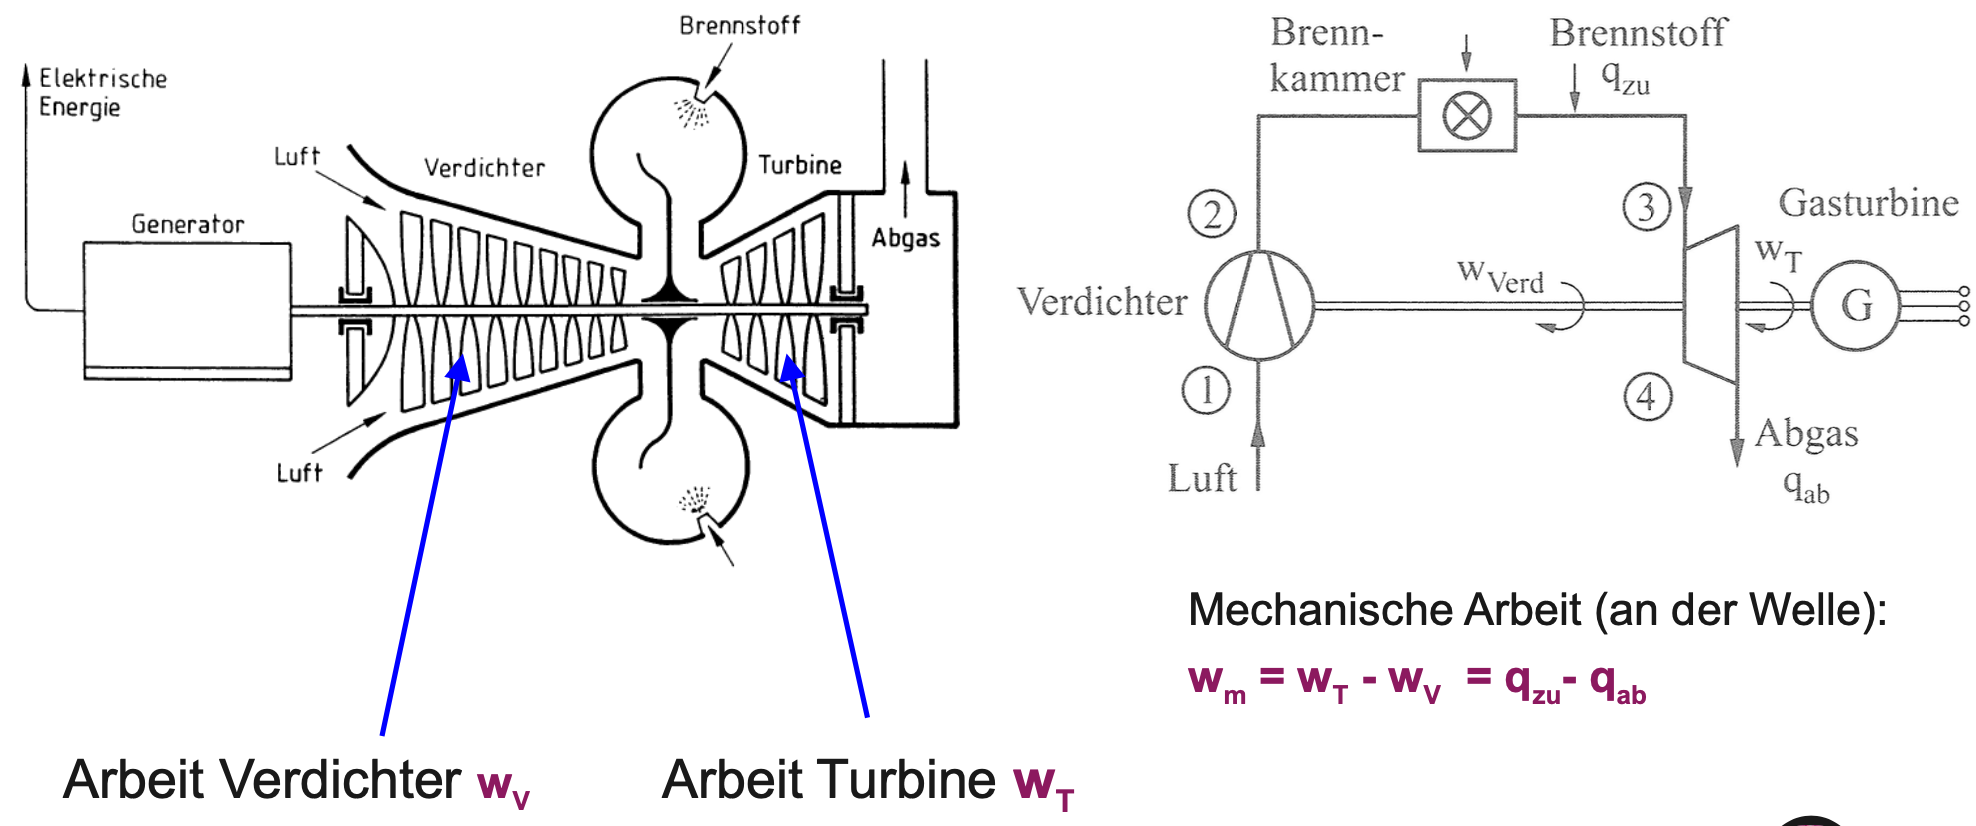
\includegraphics[width=0.9\linewidth]{images/FktprinzipGasturbine.png}
    \end{center}

\subsection{Thermodynamische Grundlage}
    \begin{center}
        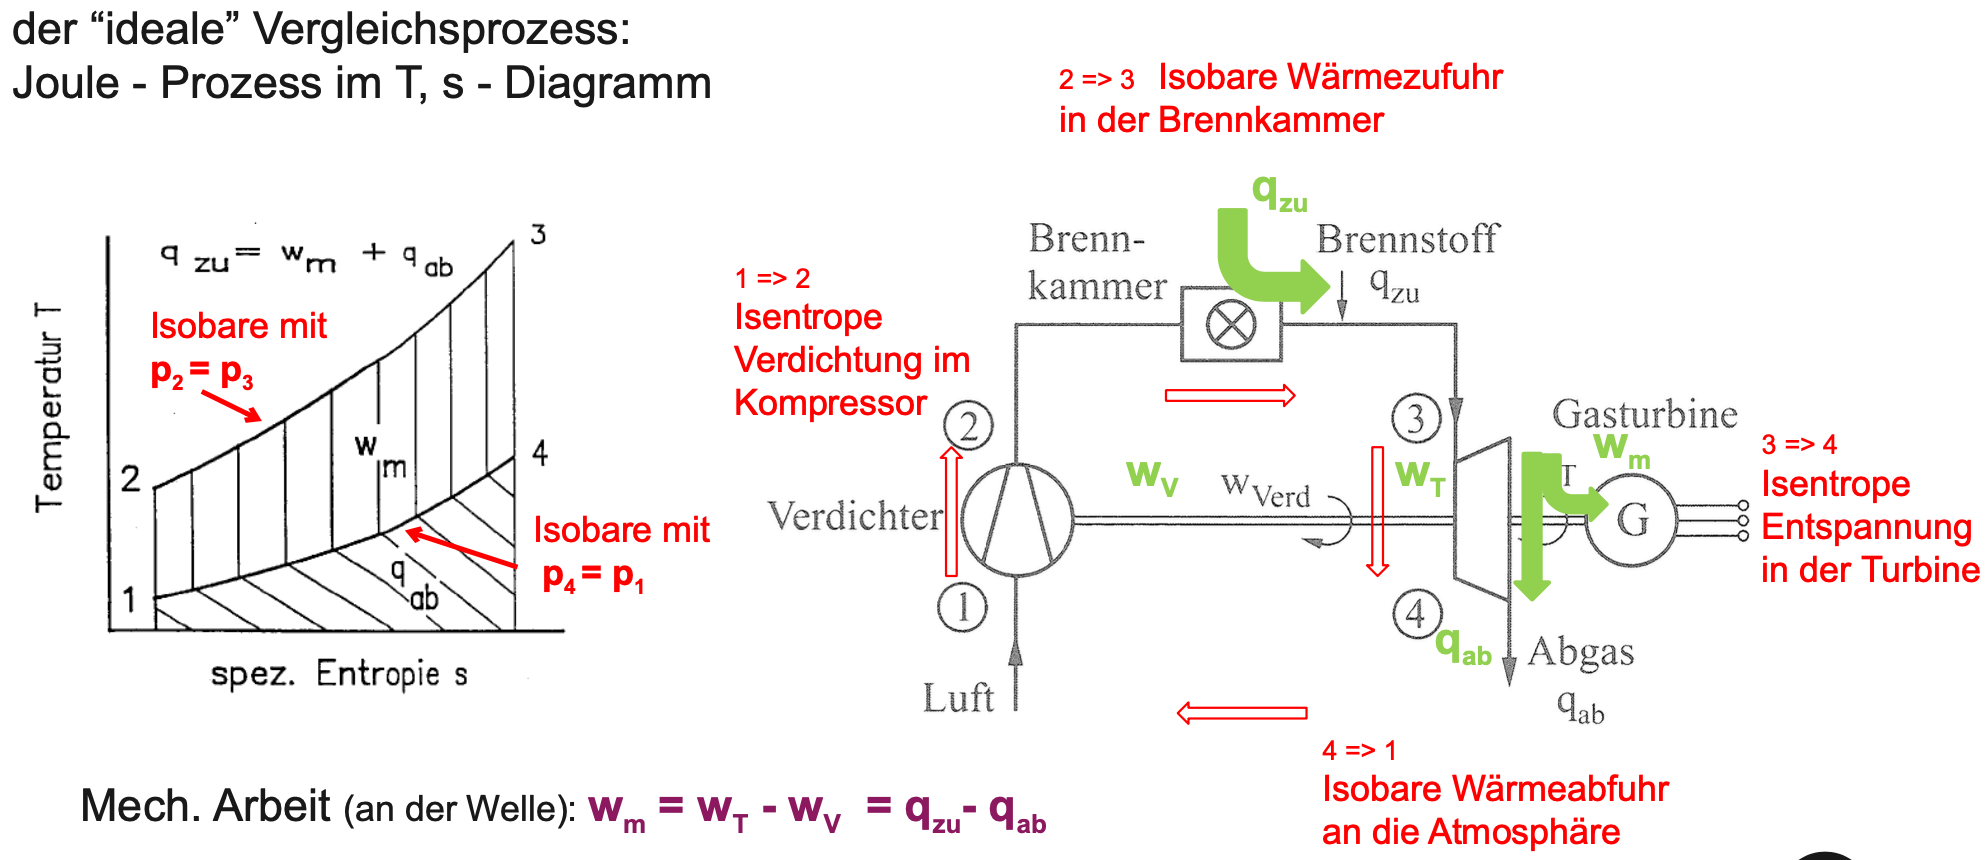
\includegraphics[width=0.9\linewidth]{images/ThermodynamischeGrundlage.png}
    \end{center}

\subsection{Gasturbine mit Luftvorwärmer}
    Verbesserung des offenen GT - Prozesses

    Vom Brennstoff aufzubringende Wärme verringert sich um $q_{WT}$, respektive die and die Umgebung abzuführende Wärme verringert sich um $q_{WT}$. Dadurch ergibt sich eine Verbesserung des therm. Wirkungsgrades.
    \begin{center}
        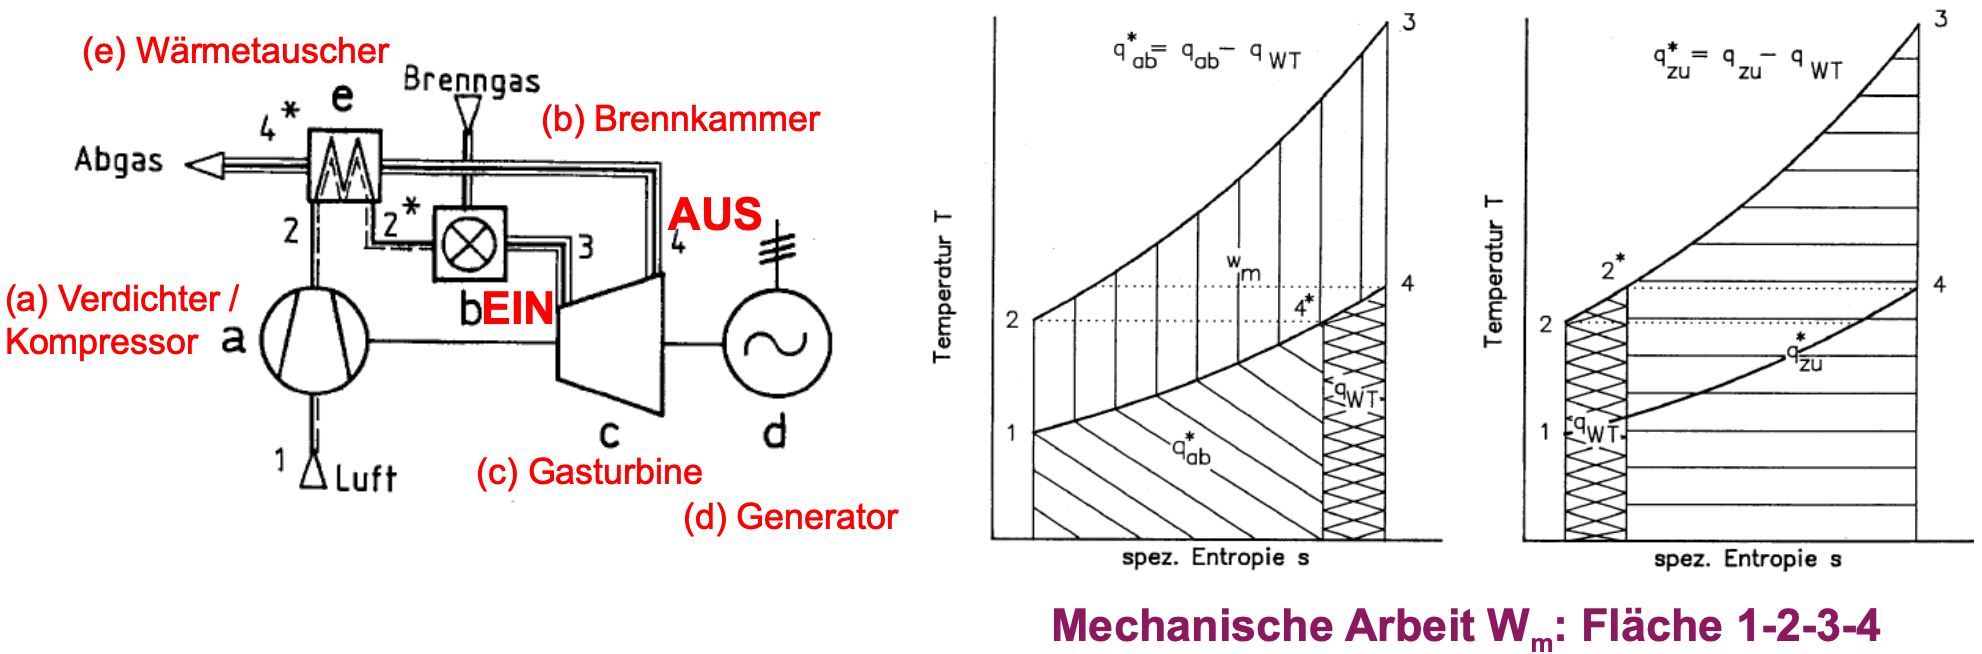
\includegraphics[width=0.9\linewidth]{images/GasturbineLuftvorwärme.png}
    \end{center}

\subsection{Gas- und Dampfturbinenkraftwerke (GuD)}
    \begin{minipage}[c]{0.5\columnwidth}
        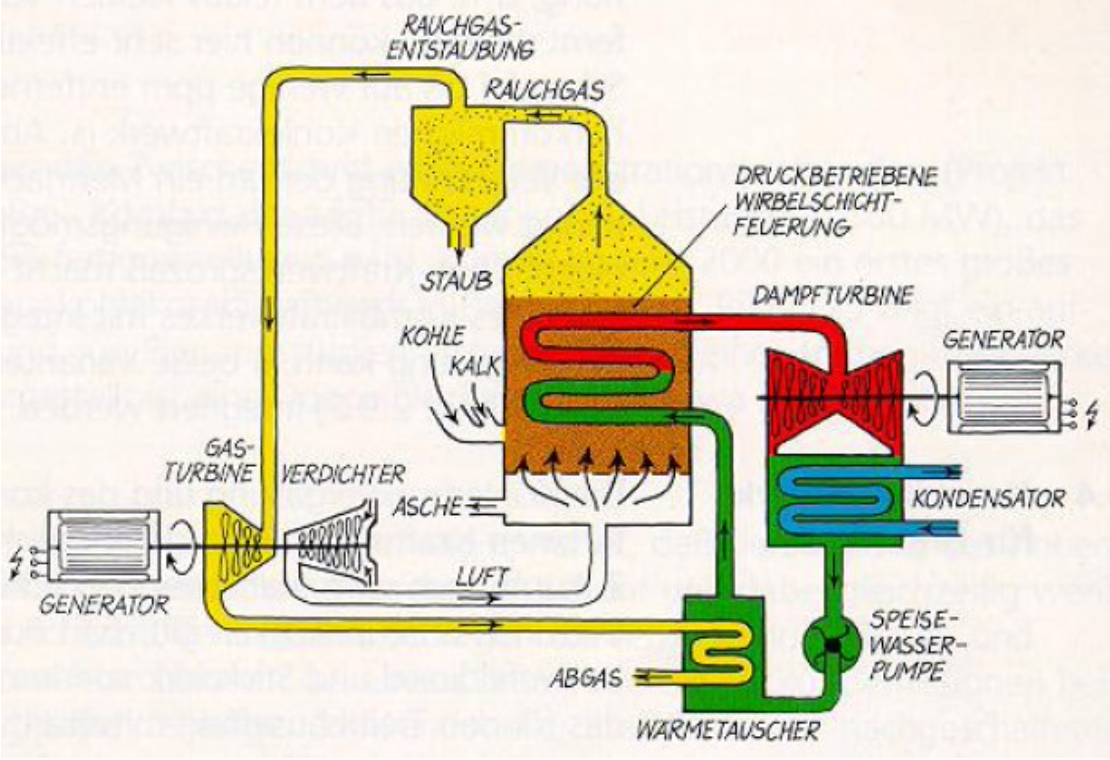
\includegraphics[width=0.9\linewidth]{images/GuD.png}
    \end{minipage}
    \begin{minipage}[c]{0.5\columnwidth}
        Eigenschaften:
        \begin{itemize}
            \item Gasturbine
            \begin{itemize}
                \item hohe Wärmeeintrittstemperatur (bis $1200\, \mathrm{^\circ C}$)
                \item hohe Wärmeaustrittstemperatur (ca. $500\, \mathrm{^\circ C}$) Dampfturbinen
            \end{itemize}
            \item Dampfturbine
            \begin{itemize}
                \item Relative niedrige Wärmeeintrittstem- peratur ($\le 550\, \mathrm{^\circ C}$)
                \item Niedrige Austrittstemperatur (ca. $40\, \mathrm{^\circ C}$)
            \end{itemize}
        \end{itemize}
    \end{minipage}

    Kombination beider Prozesse $\Rightarrow$ GuD mit hohem Wirkungsgrad

    \begin{itemize}
        \pro $5 - 10\, \mathrm{\%}$ höherer Wirkungsgrad als reine Dampf-KW
        \pro Gutes Teillastverhalten (wichtig bei Lastfolgebetrieb, Einsatz Sekundärregulierung)
        \pro Kostengünstiger Umbau älterer Dampf-KW
        \pro Geringere Abwärme
        \con $25 - 30\, \mathrm{\%}$ der zugeführten Wärme muss in Form eines hochwertigen Brennstoffes (Gas) erfolgen.
        \con Instandhaltungsaufwand an der hochbeanspruchten Gasturbine, Stillstandzeiten wegen der GT
    \end{itemize}

\subsubsection{Kombianlagen für Kraft-/Wärmekopplung (KWK)}
    Thermische Kraftwerke (Wärme- Kraft- Prinzip) geben aufgrund physikalischer Randbedingungen einen grossen Teil der Wärme als Anergie ($60 - 70\, \mathrm{\%}$) an die Umgebung ab.\\
    $\Rightarrow$ Mit der Nutzung der Abwärme kann der Gesamtwirkungsgrad wesentlich verbessert werden.

    \begin{minipage}[c]{0.5\columnwidth}
        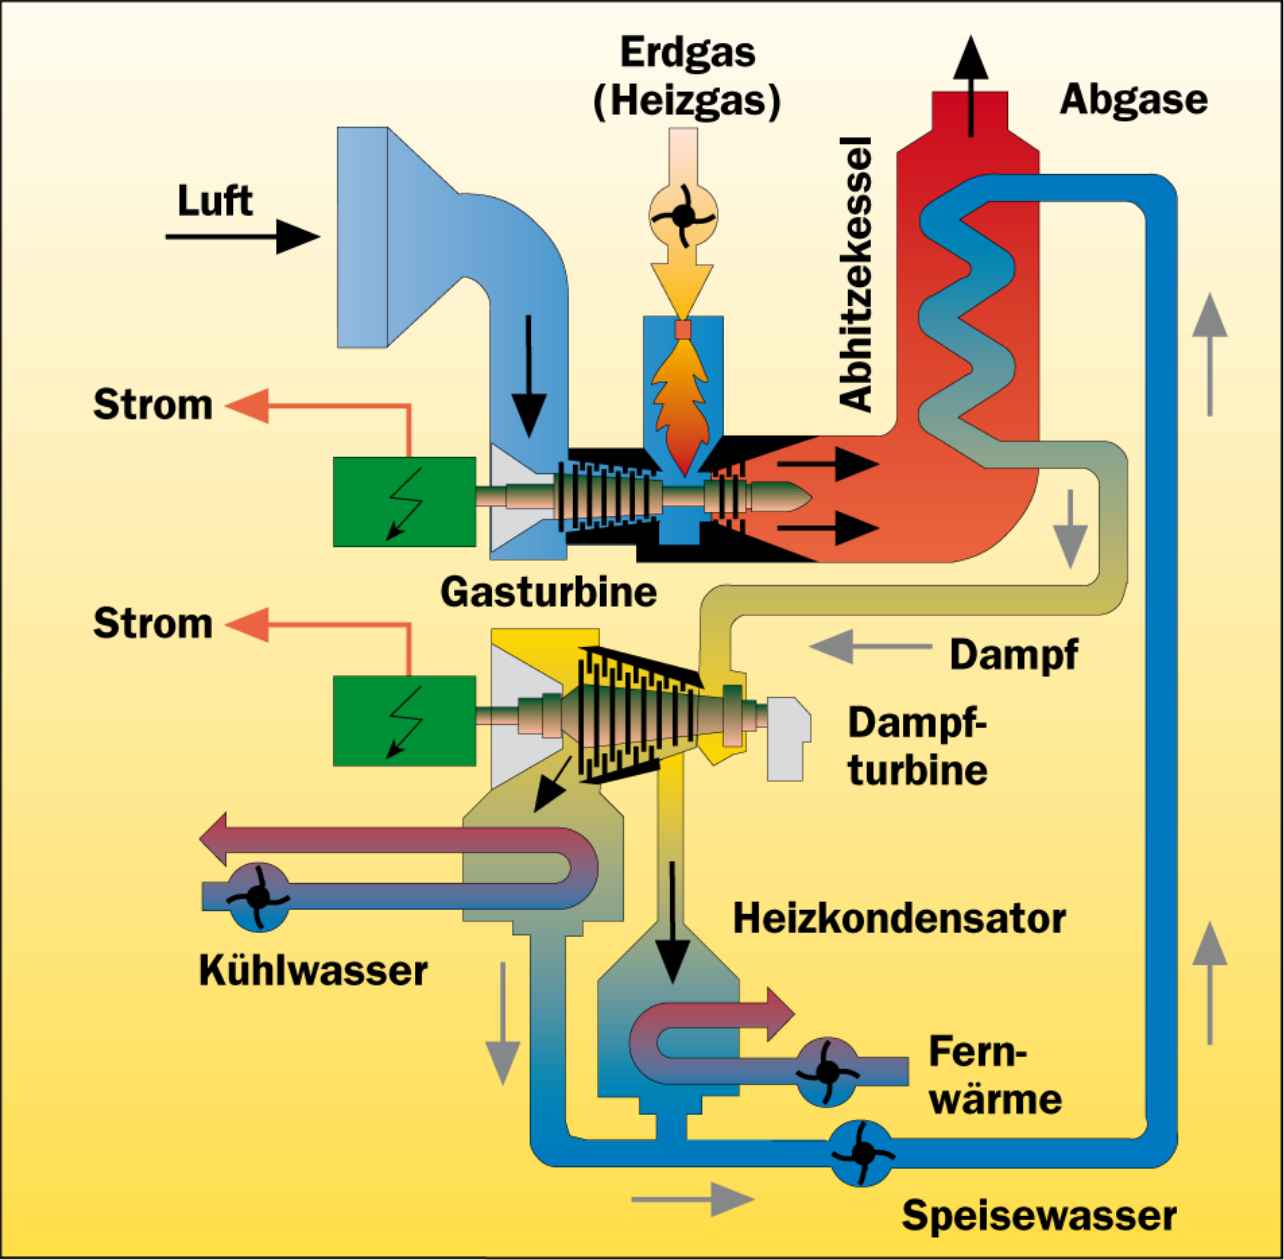
\includegraphics[width=0.9\linewidth]{images/KwK.png}
    \end{minipage}
    \begin{minipage}[c]{0.5\columnwidth}
        \begin{itemize}
            \item Abwärme wird für Prozess- oder Heizzwecke genutzt
            \item Gesamtwirkungsgrad bis $90\, \mathrm{\%}$
            \item Einen Freiheitsgrad: Strom und Wärme können nur gemeinsam erzeugt werden
            \item Zwei Freiheitsgrade: gekoppelt und ungekoppelt möglich
        \end{itemize}
        Wichtigste Anlagentypen:
        \begin{itemize}
            \item Heizkraftwerk mit Gegendruckturbine
            \item Gasturbinenheizkraftwerk
            \item Heizkraftwerk mit Verbrennungsmotor (BHKW)
            \item Auskopplung von Prozessdampf hoher Temperatur
        \end{itemize}
    \end{minipage}

    \begin{minipage}[c]{0.23\columnwidth}
        $\boxed{\eta_{\mathrm{KWK}} = \frac{W_{\mathrm{el}}+Q_{\mathrm{H}}}{W_{\mathrm{BS}}}}$
    \end{minipage}
    \hfill
    \begin{minipage}[c]{0.6\columnwidth}
        \begin{tabular}{@{} l p{4cm} l @{}}
            $[W_{\mathrm{el}}]$ & Stromproduktion \dotfill & $\mathrm{kWh}$ \\
            $[Q_{\mathrm{H}}]$  & Wärmeauskopplung \dotfill & $\mathrm{J}$ \\
            $[W_{\mathrm{BS}}]$ & Zugeführte Brennstoffenergie\dotfill & $\mathrm{J}$ \\
        \end{tabular}
    \end{minipage}

\subsection{Solarthermische Kraftwerke}
    Stromerzeugung wie bei thermischen Kraftwerken, jedoch mit Sonne
    \vspace{-4mm}
    \def\columnseprulecolor{\color{white}}
    \begin{enumerate}
        \begin{multicols}{2}
            \item Parabolrinnenkonzentrator
            \item Heliostatenfeld mit Turm
            \item Paraboloid-Dish
            \item Fresnel-Linse
        \end{multicols}
    \end{enumerate}
    \def\columnseprulecolor{\color{black}}
    \vspace{-4mm}

\subsection{Geothermische Kraftwerke}
\begin{itemize}
    \item Temperatur im Innern der Erde: \text{$5000\text{–}6000\,^\circ\text{C}$} Wärmestrom zur Oberfläche (Abkühlung)
    \item Temperaturgradient: $3\, \mathrm{K}$ pro $100\, \mathrm{m}$
    \item Geothermische Anomalien → neben der Wärmeleitung noch Konvektion bzw. Wärmetransport durch Materialtransport (Aufstieg von glutflüssigem Magmas oder aufwärtsgerichtete Grundwasserbewegungen, aber meist in Erdbebengebiten)
    \item Umweltbeeinflussung:
    \begin{itemize}
        \item chemisch agressive und z.T. giftige Bestandteile ->Bauteiele müssen Korrisionsbeständig sein
        \item Zurückpumpen, verhindert auch das Absenken des Bodens
    \end{itemize}
\end{itemize}

\subsection{Verstromung von Biomasse}
Energiegewinnung aus Pflanzen oder Pflanzenresten
Verwendete Materialien:
\begin{itemize}
    \item eigens dafür kultivierte landwirtschaftliche Nutzpflanzen wie Mais oder Raps
    \item schnell wachsende Gehölze
    \item Abfall- und Reststoffe aus Landwirtschaft, Haushalten und Industrie (beispielsweise Hackschnitzel aus der
Holzindustrie, Altfett aus der Lebensmittelherstellung, aber auch Klärschlamm)

\end{itemize}

\newcolumn % done
        \input{sections/45_Windenergie_Windkraftwerke.tex} % done
        \section{Netze Allgemein}

\subsubsection{Stromnetz früher}
    \begin{center}
        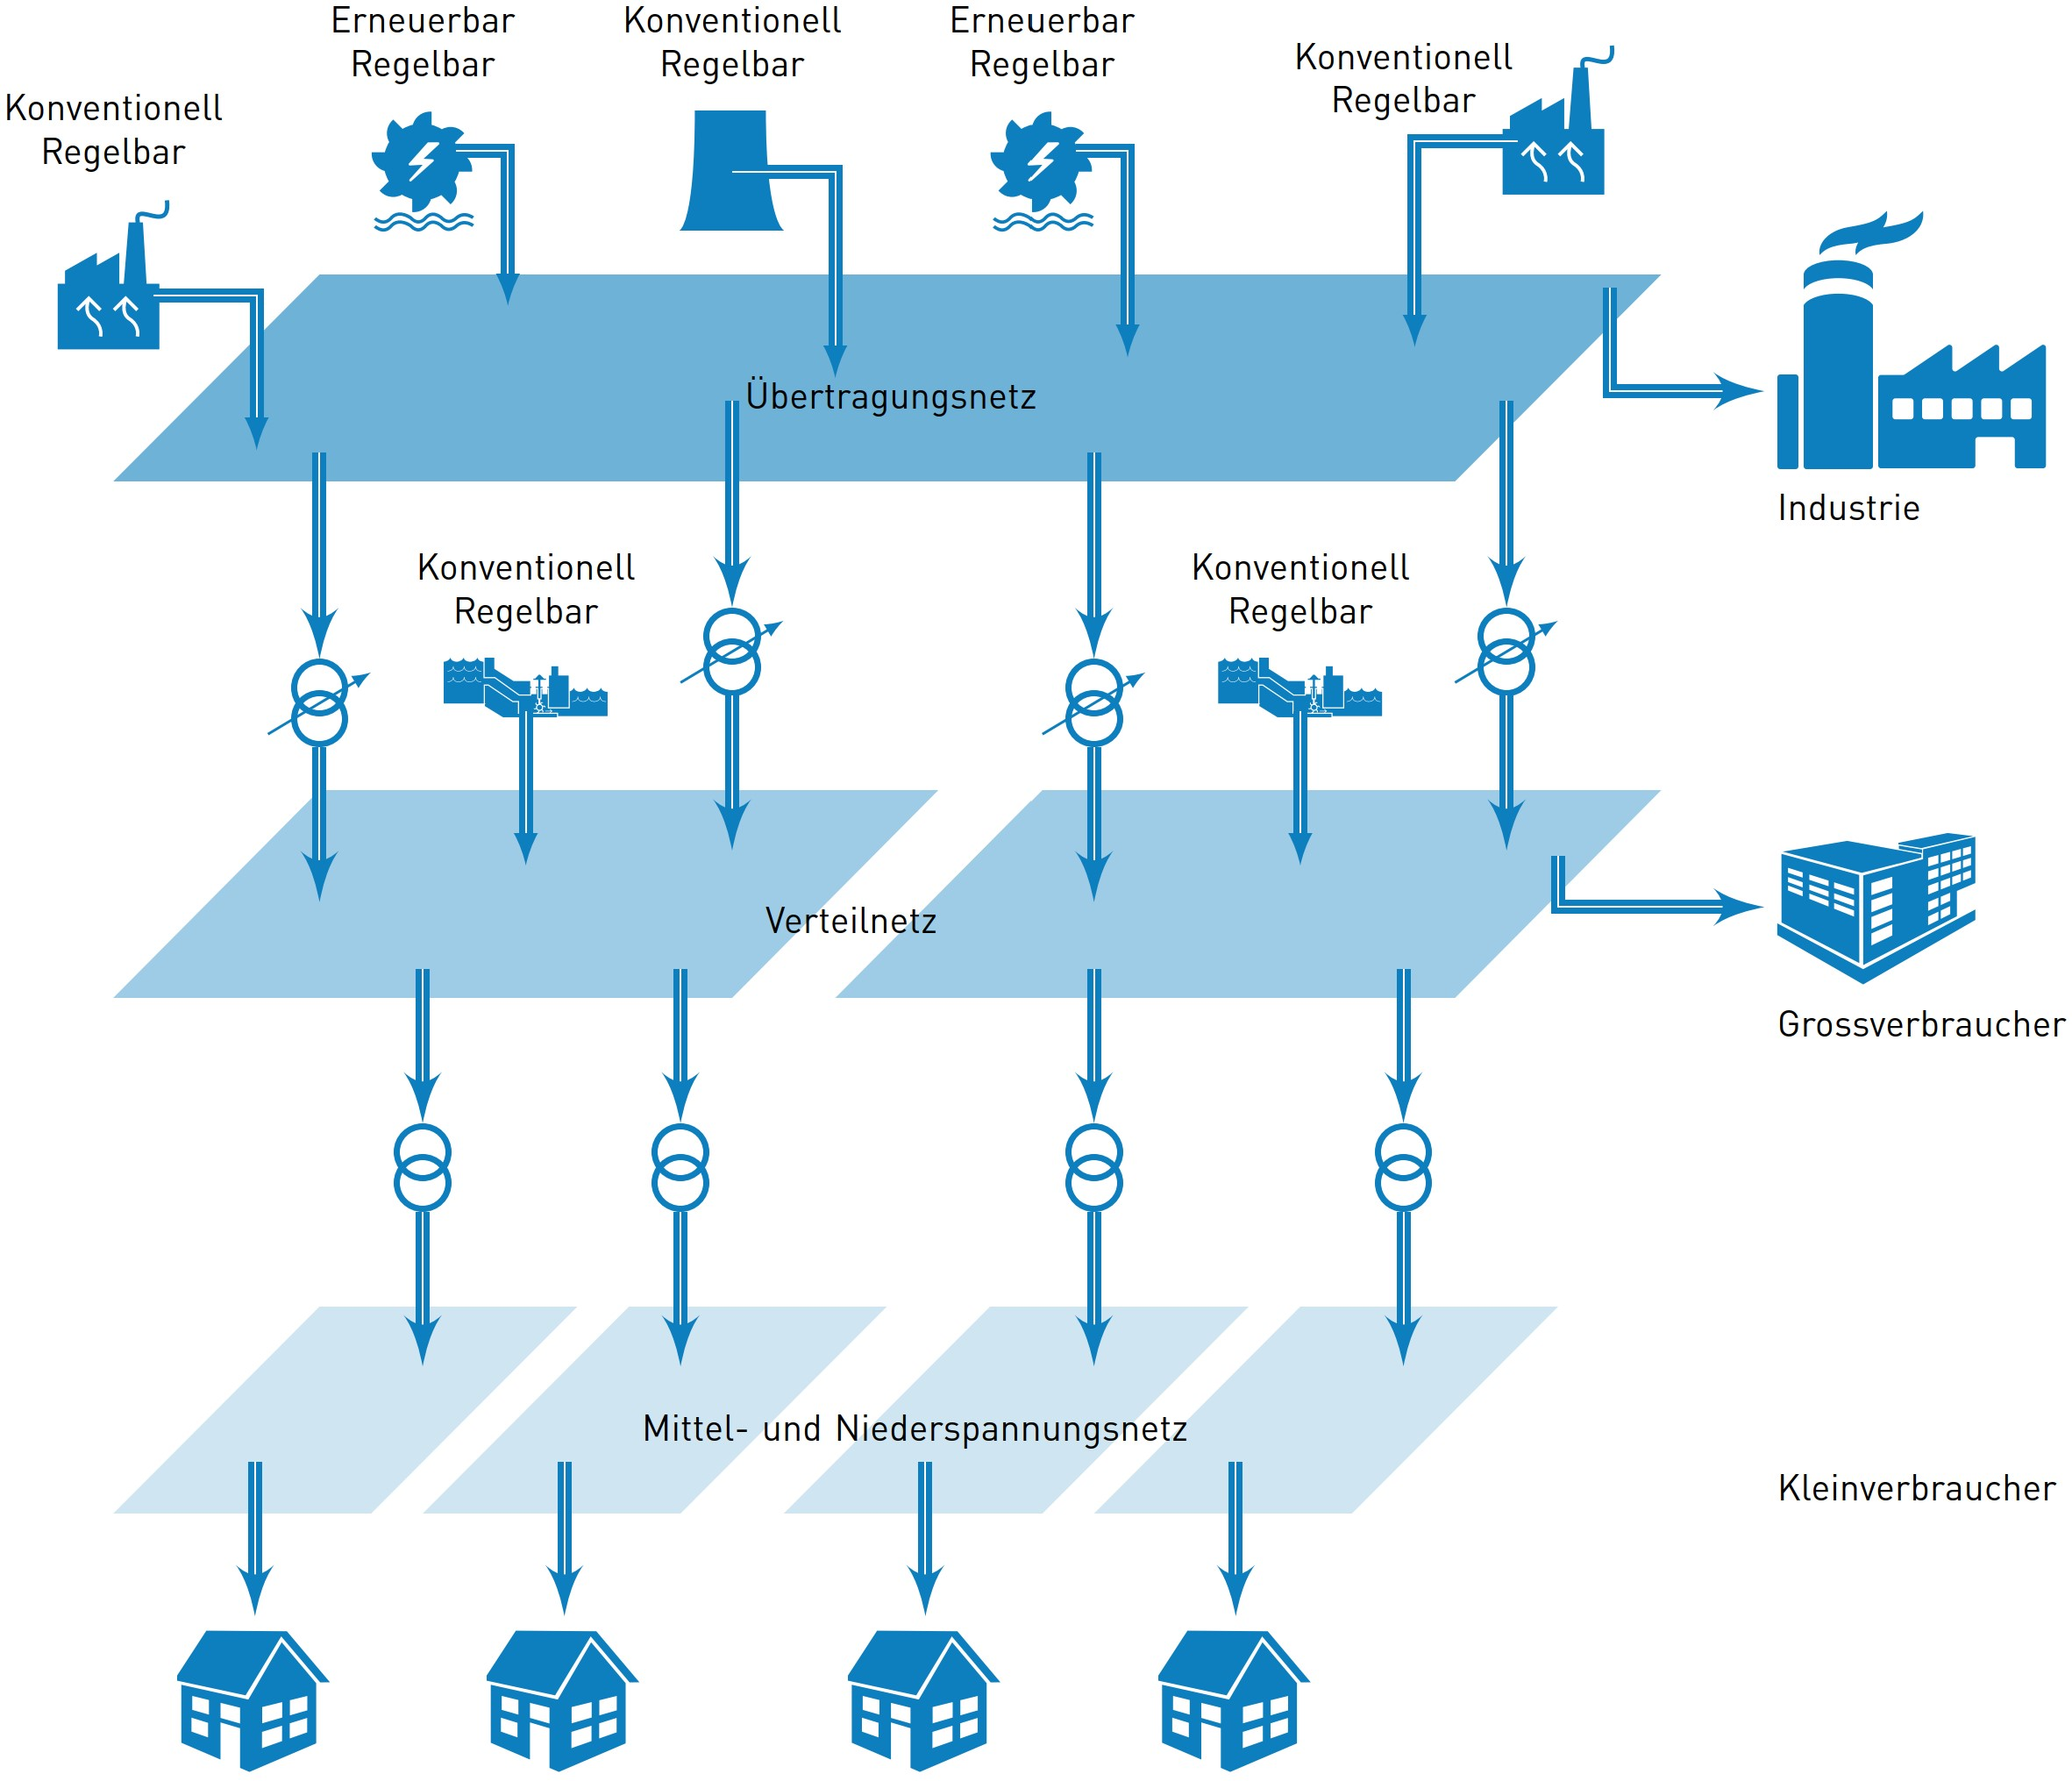
\includegraphics[width=0.95\columnwidth, align=c]{images/Aufgabe_des_Netzes_früher.jpg}
    \end{center}

\subsubsection{Stromnetz heute}
    \begin{center}
        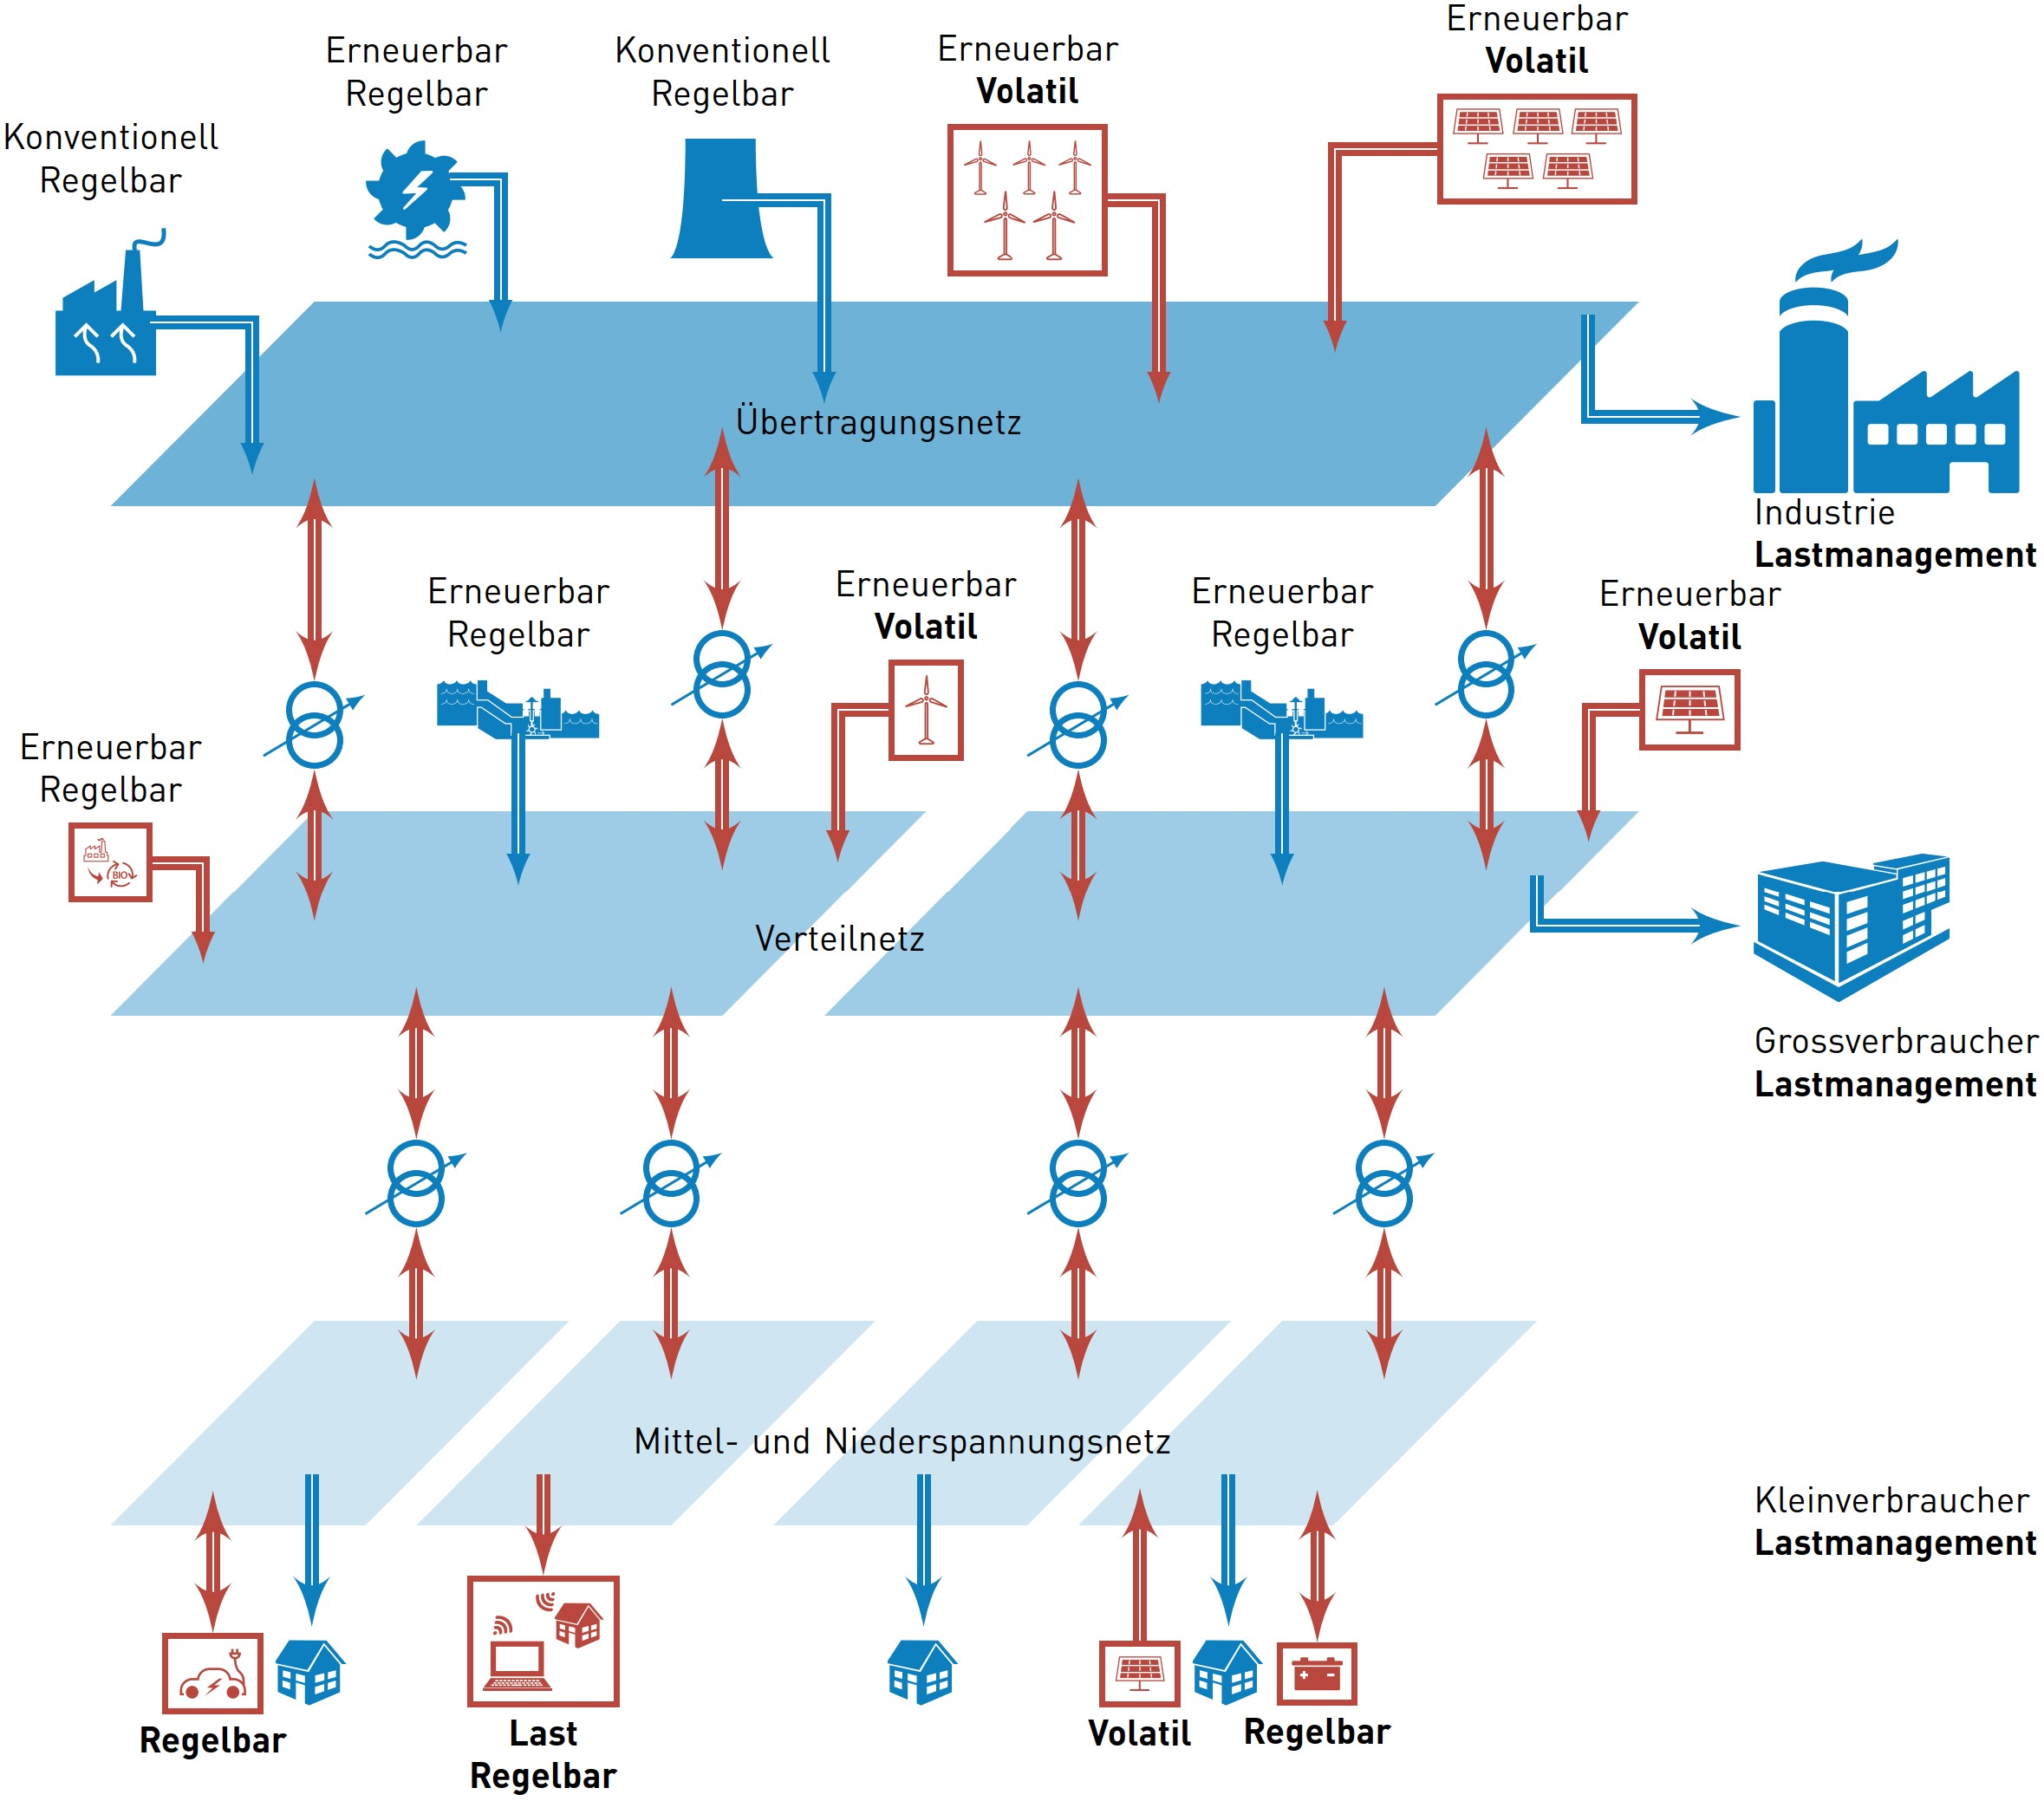
\includegraphics[width=0.95\columnwidth, align=c]{images/Aufgabe_des_Netzes_heute.jpg}
    \end{center}

\subsection{Interessen der Erzeuger}
    \begin{minipage}[t]{0.49\columnwidth}
        \begin{itemize}
            \item \textbf{Erzeuger}
            \begin{itemize}
                \item Freier Netzzugang
                \item Hohe Verfügbarkeit:
                \item[] produzierte Leistung kann jederzeit abgeführt werden
                \item Geringe Kosten
            \end{itemize}
        \end{itemize}
    \end{minipage}
    \hfill
    \begin{minipage}[t]{0.49\columnwidth}
        \begin{itemize}
            \item \textbf{Verbraucher}
            \begin{itemize}
                \item Netzanschluss
                \item Hohe Versorgungssicherheit 
                \item[] und -qualität
                \item Geringe Kosten
            \end{itemize}
        \end{itemize}
    \end{minipage}

    % \begin{itemize}
    %     \item \textbf{Erzeuger}
    %     \begin{itemize}
    %         \item Freier Netzzugang
    %         \item Hohe Verfügbarkeit: produzierte Leistung kann jederzeit abgeführt werden
    %         \item Geringe Kosten
    %     \end{itemize}
    %     \item \textbf{Verbraucher}
    %     \begin{itemize}
    %         \item Netzanschluss
    %         \item Hohe Versorgungssicherheit und -qualität
    %         \item Geringe Kosten
    %     \end{itemize}
    % \end{itemize}

\subsection{Anforderungen an das Stromnetz}
    \begin{minipage}[t]{0.49\columnwidth}
        \begin{itemize}
            \item Hohe Verfügbarkeit
            \item Hohe Versorgungsqualität
            \item Sicherheit
        \end{itemize}
    \end{minipage}
    \hfill
    \begin{minipage}[t]{0.49\columnwidth}
        \begin{itemize}
            \item Wirtschaftlichkeit
            \item Diskriminierungsfreiheit
            \item Transparenz
        \end{itemize}
    \end{minipage}

% \begin{itemize}
%     \item Hohe Verfügbarkeit
%     \item Hohe Versorgungsqualität
%     \item Sicherheit
%     \item Wirtschaftlichkeit
%     \item Diskriminierungsfreiheit
%     \item Transparenz
% \end{itemize}

\subsection{Herausforderungen}
    \begin{itemize}
        \item Volatil: Angebot und Nachfrage nicht vorhersehbar
        \item Angebot und Nachfrage muss immer gleich sein
        \item PV und Wind sind nur runterregelbar (Wasser- und Atomkraft sind auch raufregelbar)
    \end{itemize}

 % done
        \section{Netzebenen}
    \begin{center}
        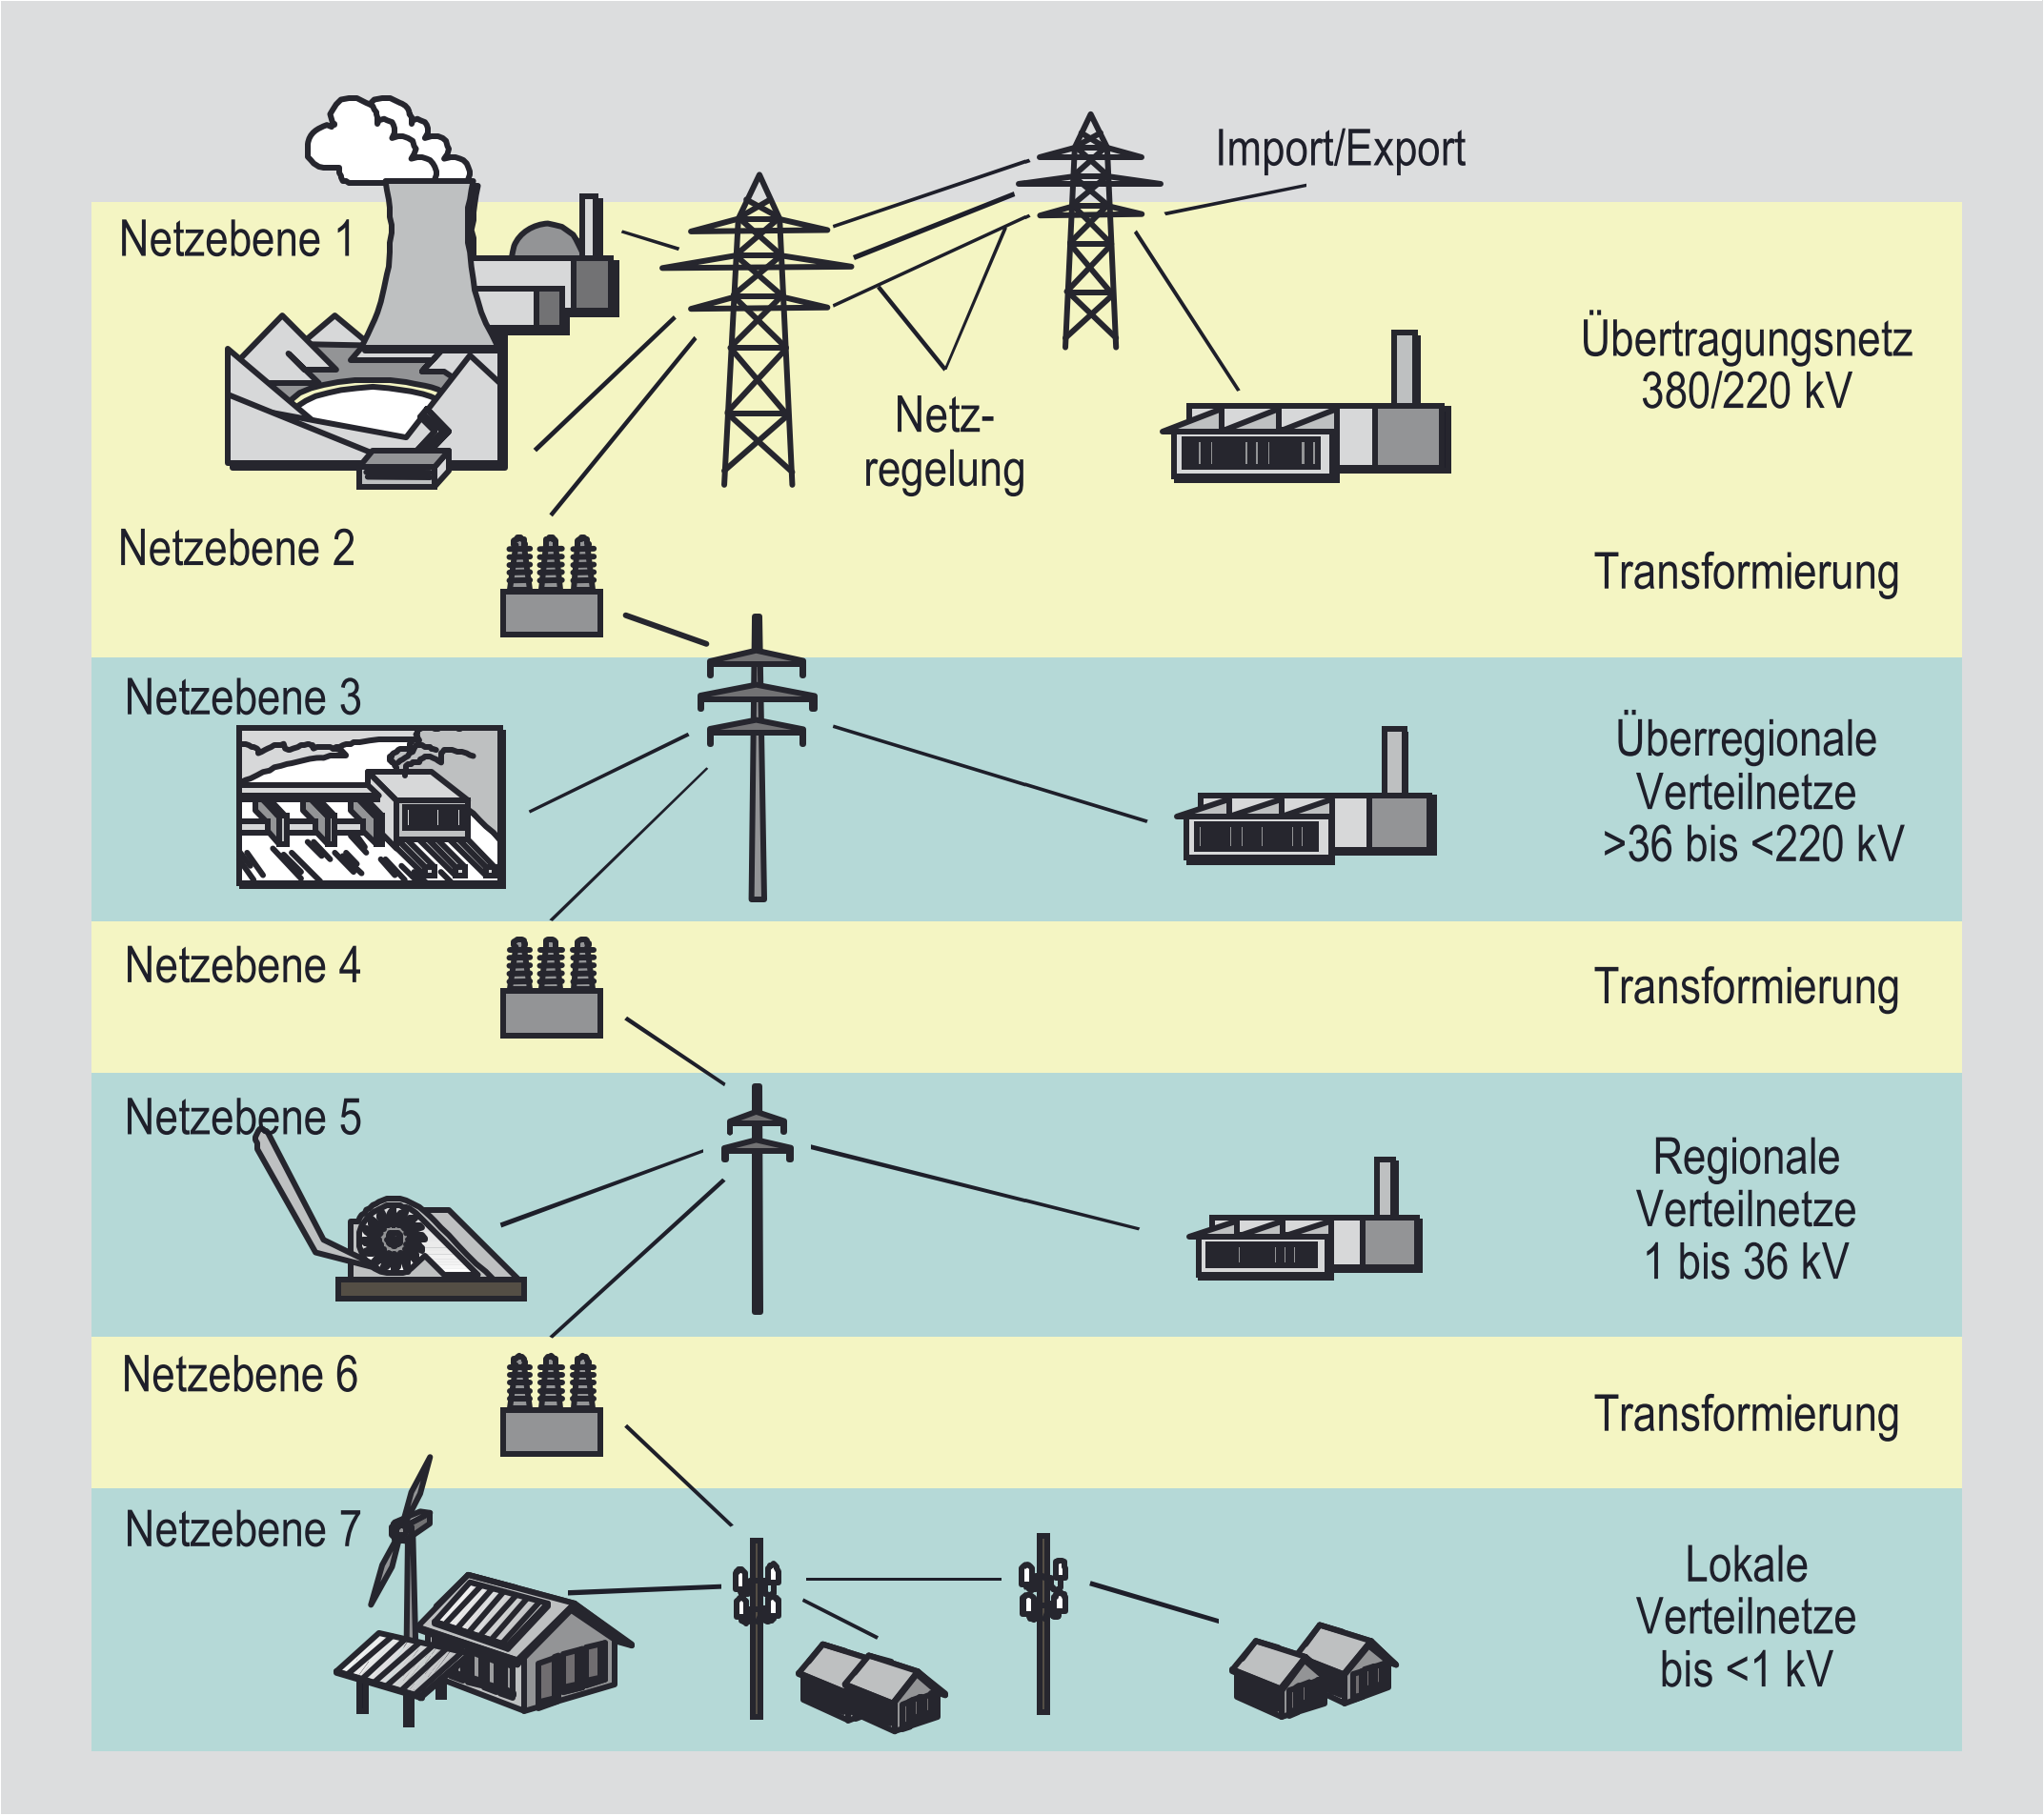
\includegraphics[width=0.95\columnwidth, align=c]{images/Netzebenen_1.png}
    \end{center}

    \begin{center}
        \begin{tabular}{>{\bfseries}l l l}
            \toprule
            Spannungsebene & Spannungsbereich & Leistung \\
            \midrule
            Höchstspannung   & 380 kV, 220 kV         & > 300 MVA \\
            Hochspannung     & 150 kV bis 50 kV       & < 100 MVA \\
            Mittelspannung   & 36 kV bis 6 kV         & < 30 MVA \\
            Niederspannung   & 0{,}4 kV               & < 1 MVA \\
            \bottomrule
        \end{tabular}
    \end{center}

\subsection{NE1: Übertragungsnetz (380\,kV, 220\,kV)}
    \begin{minipage}[t]{0.5\columnwidth}
        \begin{itemize}
            \item \textbf{Zweck}
            \begin{itemize}
                \item Abtransport der großen KW-Leistungen (typ. > 300\,MVA)
                \item Versorgung der Verteilnetze
                \item Weiträumiger Energietransport
                \item Internat. Verbundbetrieb, Energieaustausch
            \end{itemize}
        \end{itemize}
    \end{minipage}%
    \hfill
    \begin{minipage}[t]{0.49\columnwidth}
        \begin{itemize}
            \item \textbf{Ausdehnung:} national, international
            \item \textbf{Topologie:} (stark) vermaschtes Netz
            \item \textbf{Technologie:} fast nur Freileitungen
        \end{itemize}
    \end{minipage}

\subsubsection{Schweizer Stromübertragungsnetz (Daten 2014)}
    \begin{center}
        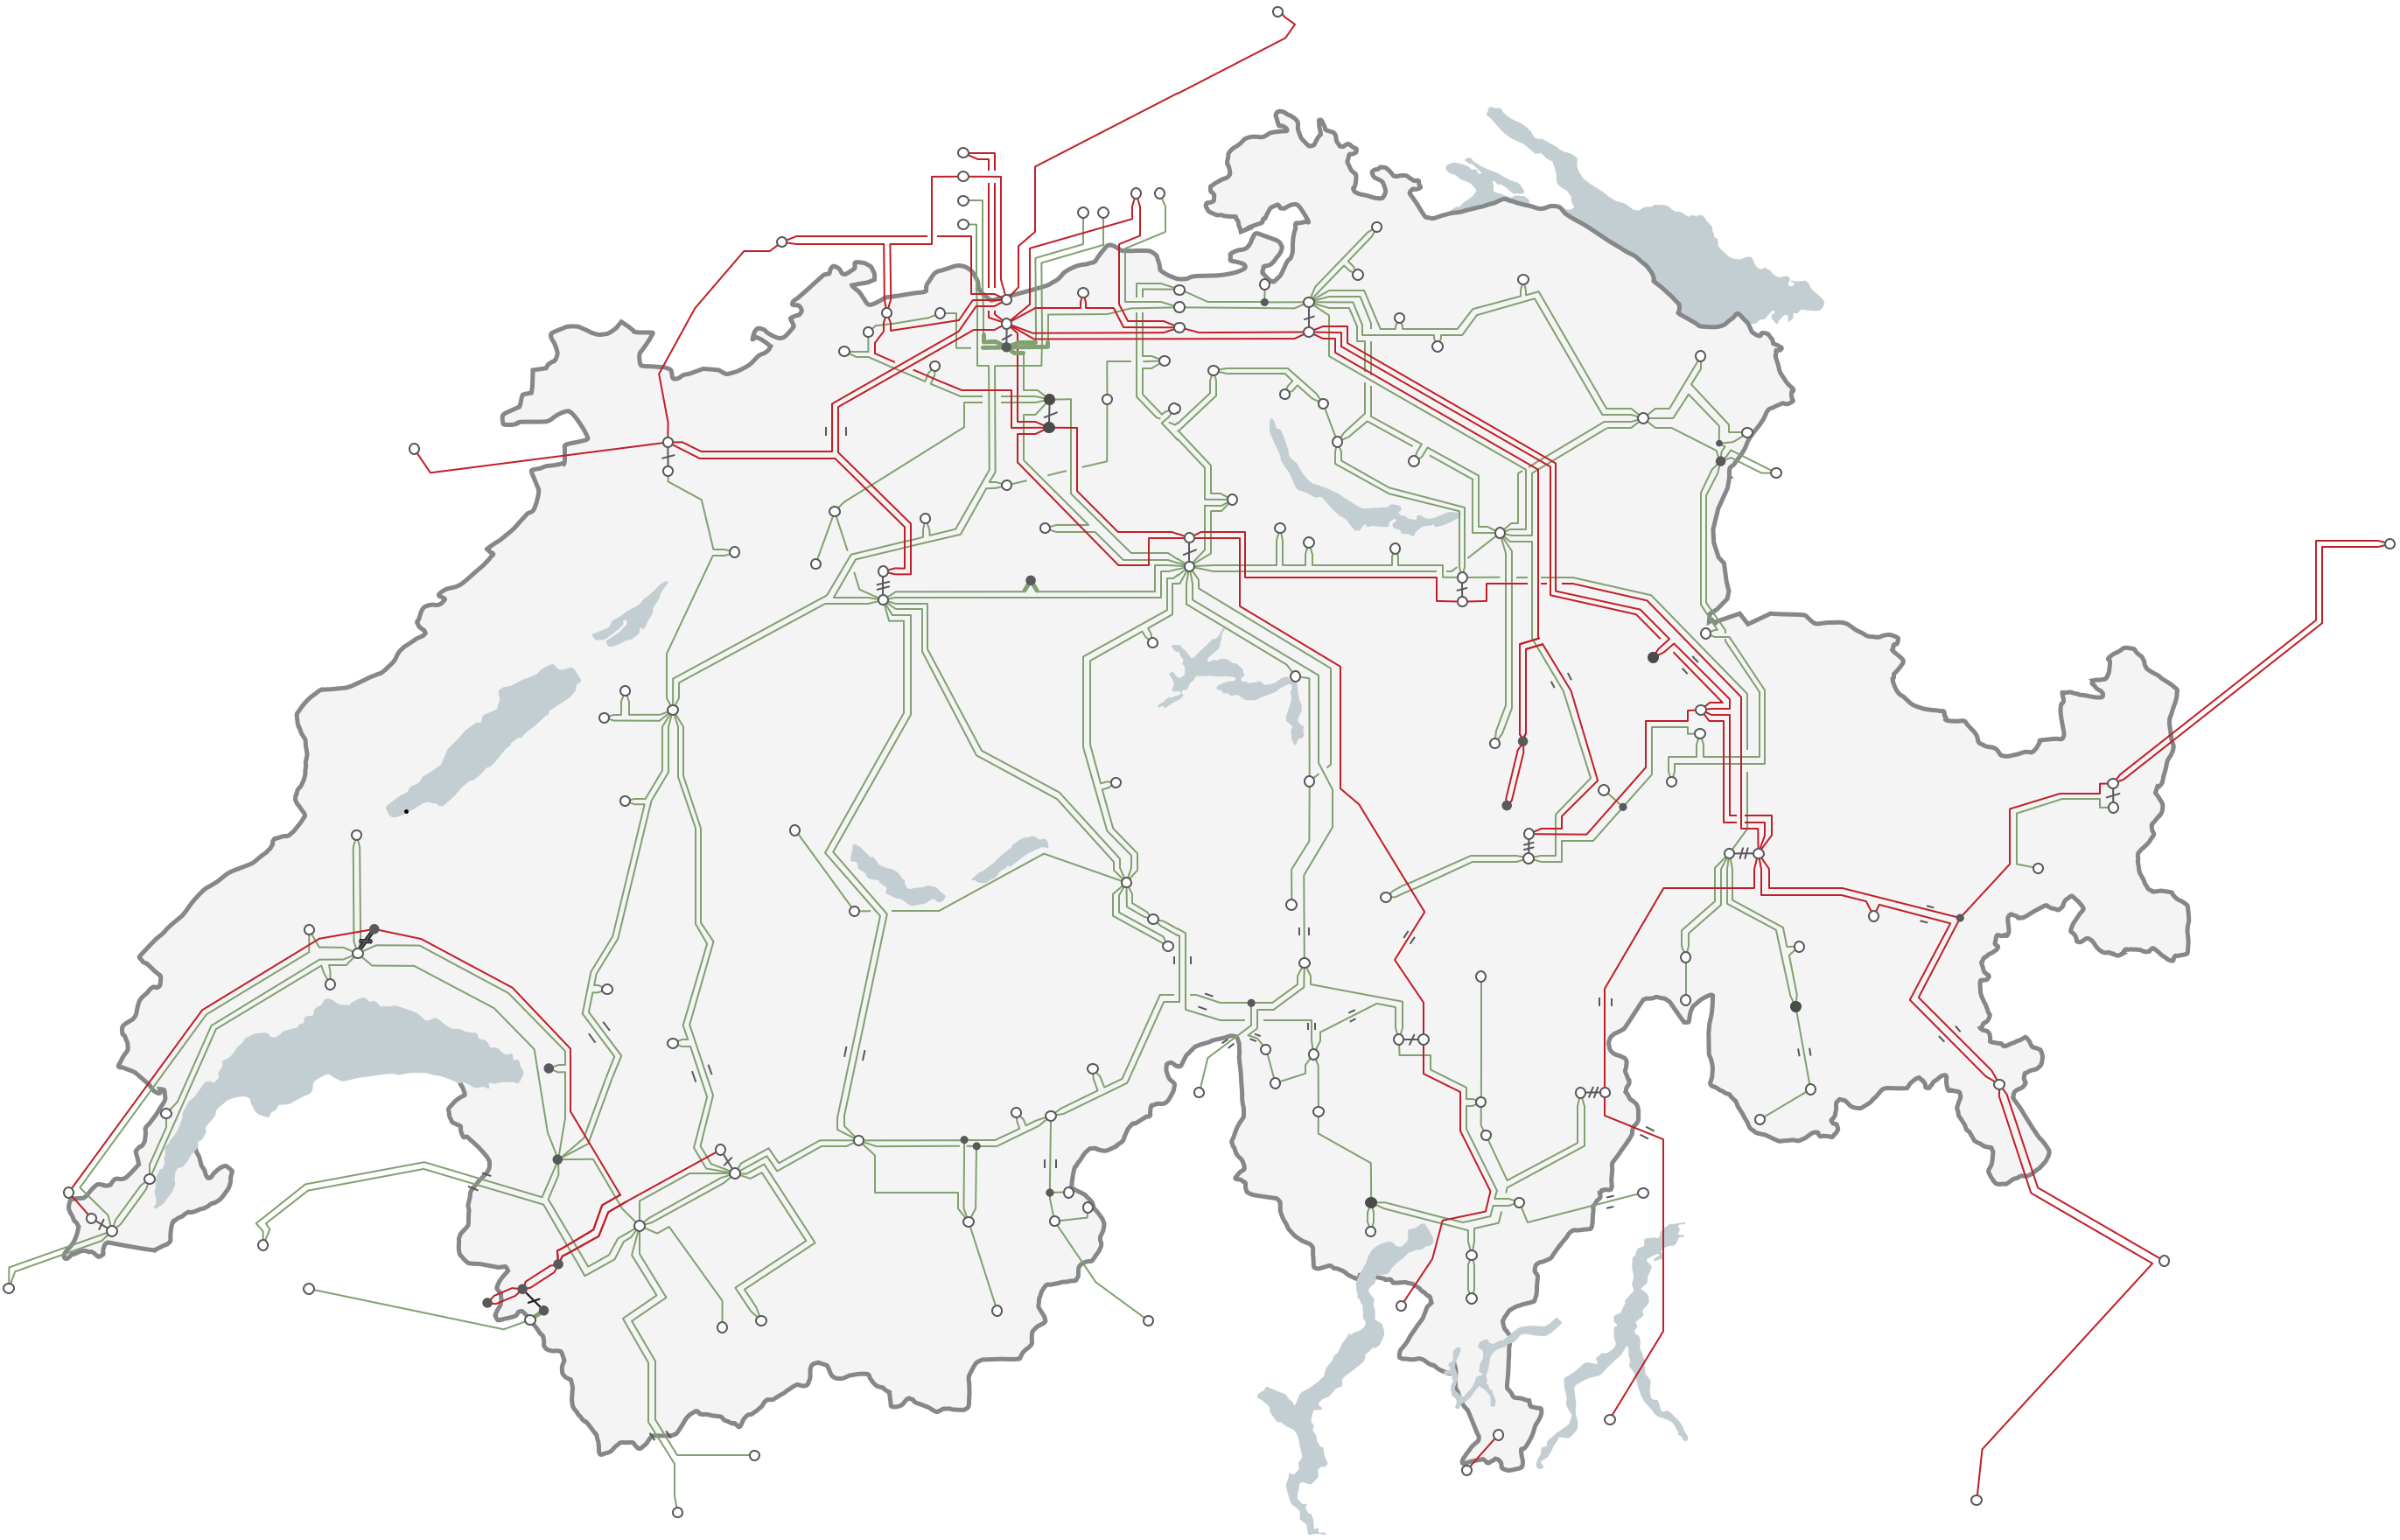
\includegraphics[width=0.95\columnwidth, align=c]{images/Schweizer_übertragungsnetz.png}
    \end{center}

    \begin{itemize}
        \item Gesamtlänge Übertragungsnetz Inland: 6700 km
        \begin{itemize}
            \item Länge 380\,kV: 1780 km
            \item Länge 220\,kV: 4920 km
        \end{itemize}
        
        \item Gesamtzahl Leitungen im Übertragungsnetz: 246
        \begin{itemize}
            \item Leitungen 380\,kV: 48
            \item Leitungen 220\,kV: 198
        \end{itemize}
        
        \item Anzahl Netzübergänge in das Ausland: 41
    \end{itemize}

\subsubsection{Entso-E}
    \begin{minipage}[t]{0.39\columnwidth}
        \textbf{Koordination von:}
        \begin{itemize}
            \item Systembetrieb
            \item Marktlösungen
            \item Systementwicklung
        \end{itemize}
    \end{minipage}
    \hfill
    \begin{minipage}[t]{0.6\columnwidth}
        \centering \vspace{-0.7\baselineskip}
        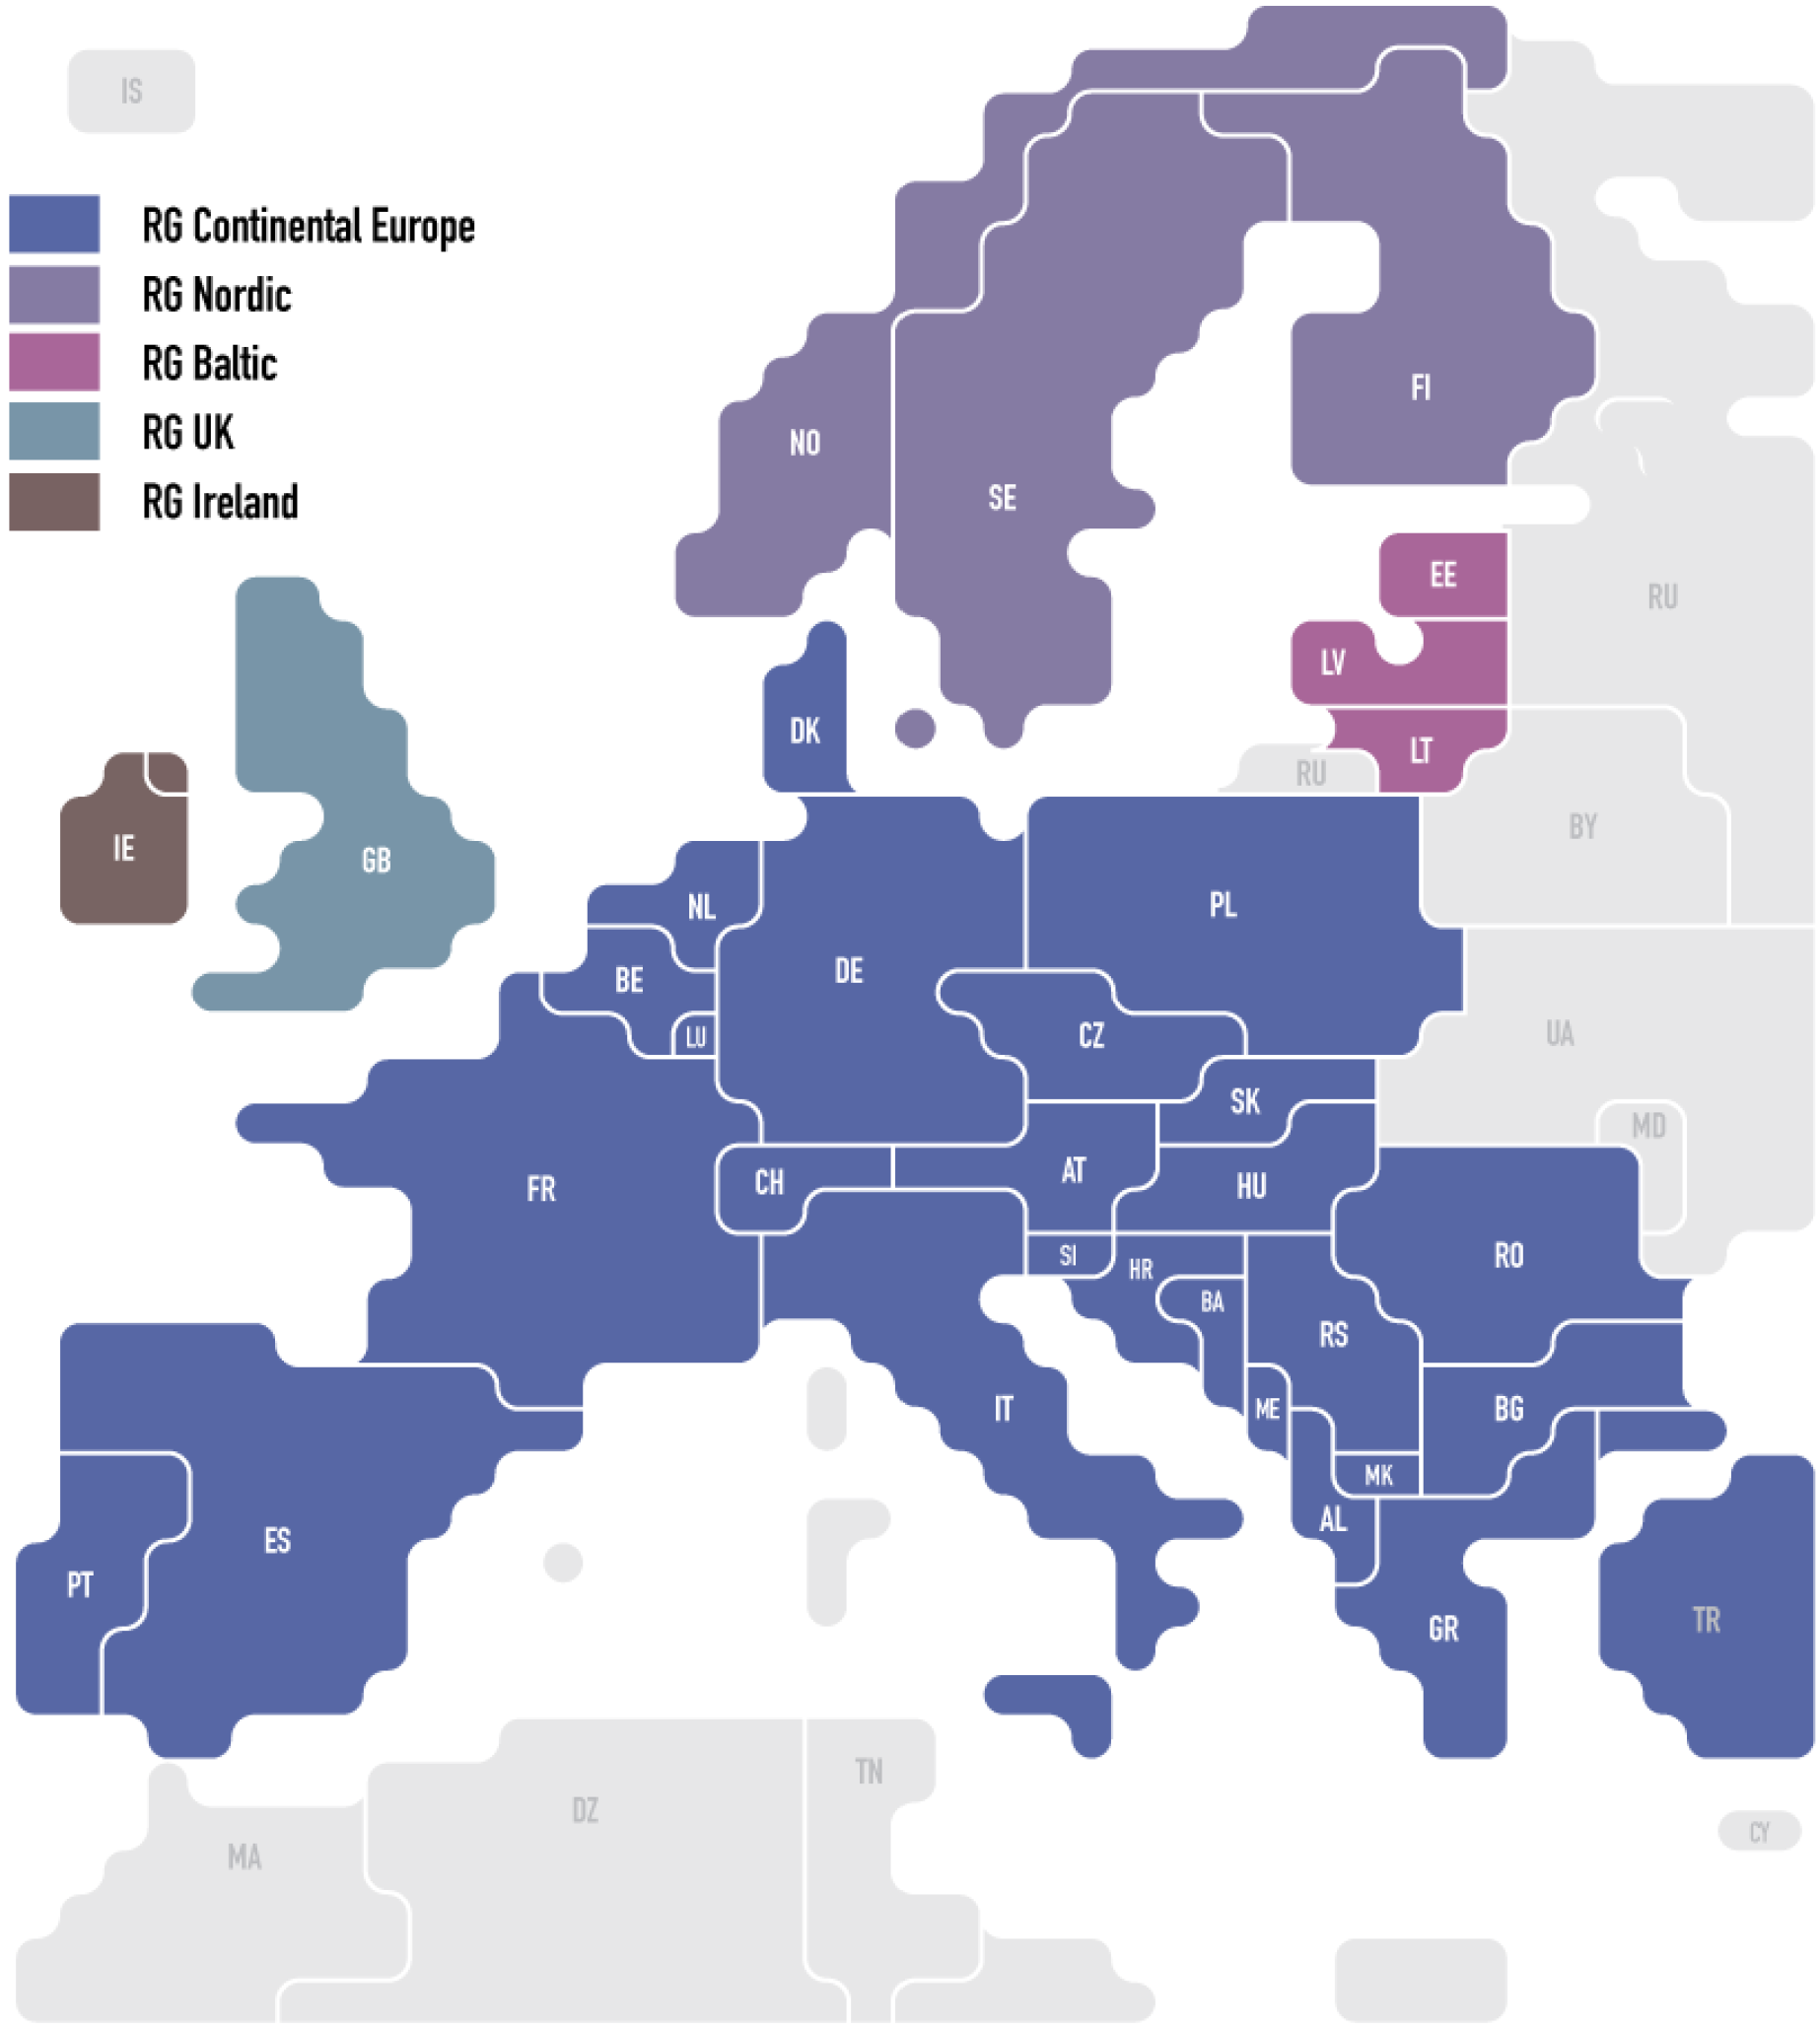
\includegraphics[width=0.8\textwidth]{images/Entso_E.png}
    \end{minipage}%

    % \begin{center}
    %     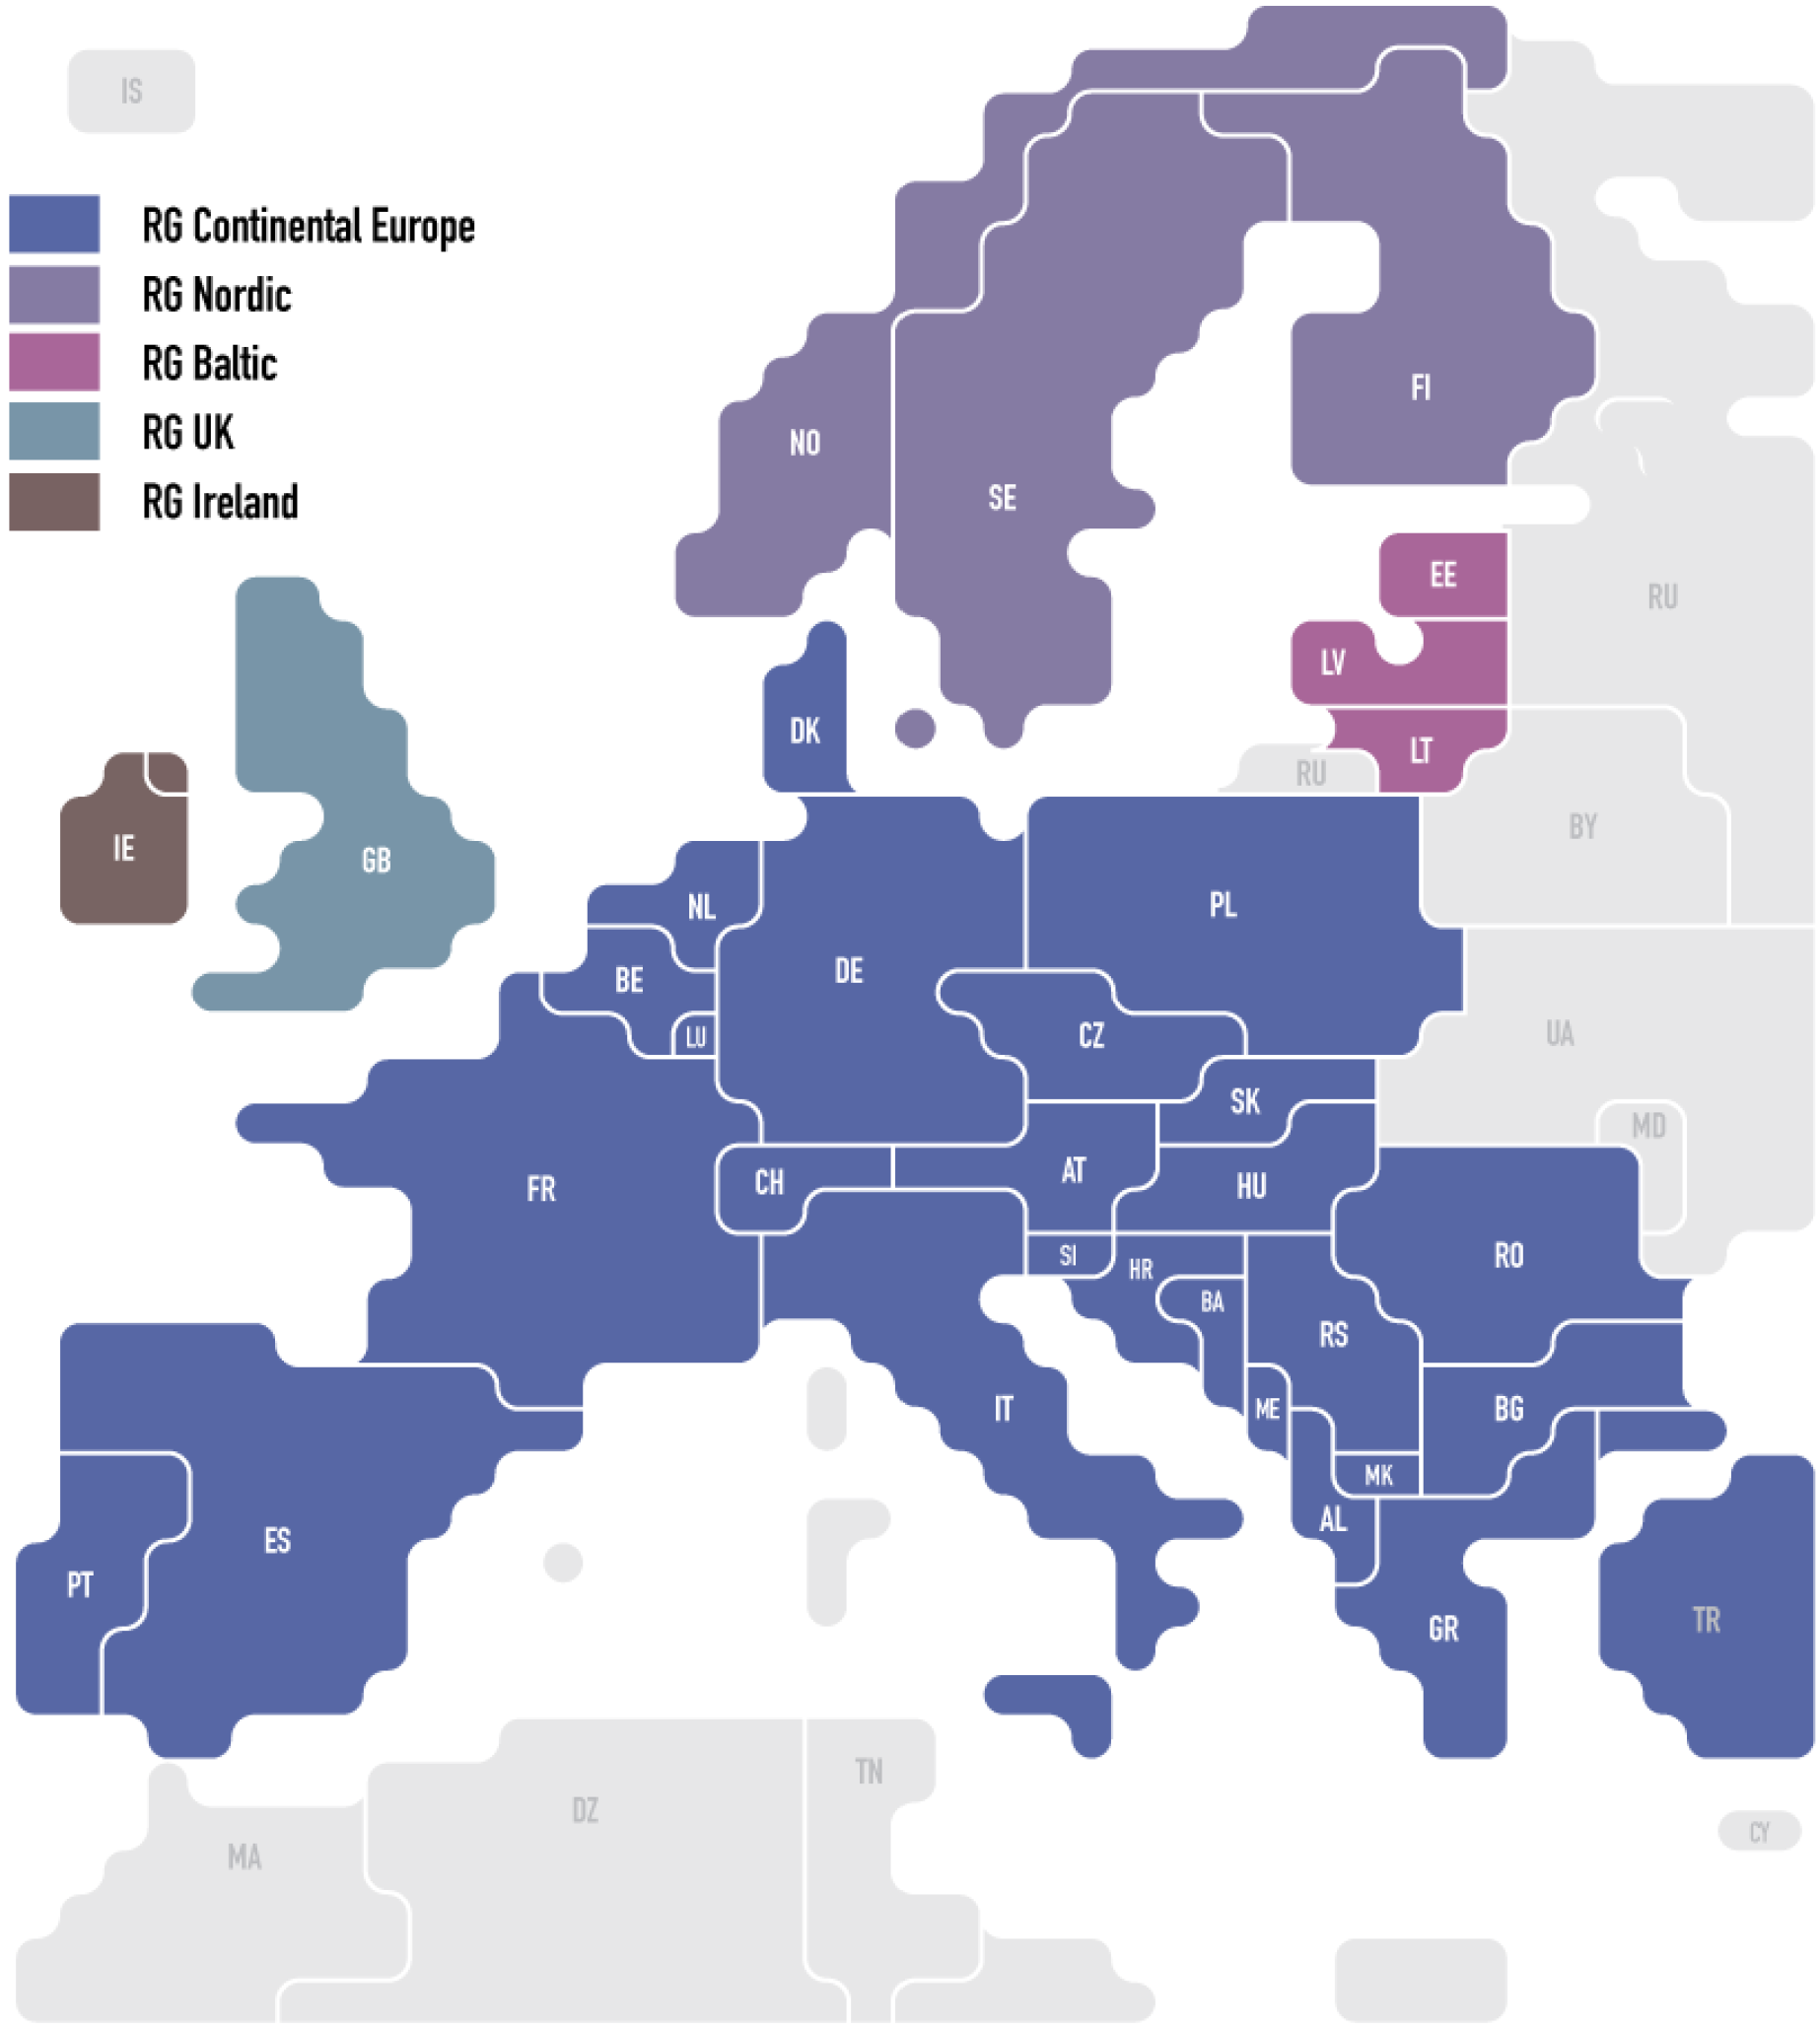
\includegraphics[width=0.75\columnwidth, align=c]{images/Entso_E.png}
    % \end{center}

    % \begin{itemize}
    %     \item koordinierter Systembetrieb
    %     \item koordinierte Marktlösungen
    %     \item koordinierte Systementwicklung
    % \end{itemize}

\subsection{NE3: Überregionales Verteilnetz (150, 132, 60\,kV)}
    \begin{minipage}[t]{0.5\columnwidth}
        \begin{itemize}
            \item \textbf{Zweck}
            \begin{itemize}
                \item Abtransport mittlerer Kraftwerksleistungen (typ. 100\,MVA)
                \item Anschluss großer Industriekunden
                \item Überregionale Verteilung
            \end{itemize}
        \end{itemize}
    \end{minipage}%
    \hfill
    \begin{minipage}[t]{0.49\columnwidth}
        \begin{itemize}
            \item \textbf{Ausdehnung:} mehrere Kantone
            \item \textbf{Topologie:} (leicht) vermascht oder Ring
            \item \textbf{Technologie:} vorwiegend Freileitungen
        \end{itemize}
    \end{minipage}
    % \begin{itemize}
    %     \item Zweck
    %     \begin{itemize}
    %         \item Abtransport mittlerer Kraftwerksleistungen (typ. 100 MVA)
    %         \item Anschluss großer Industriekunden
    %         \item Überregionale Verteilung
    %     \end{itemize}
    %     \item Ausdehnung: mehrere Kantone
    %     \item Topologie: (leicht) vermaschtes Netz oder Ringnetz
    %     \item Technologie: vorwiegend Freileitungen
    % \end{itemize}

\subsection{NE5: Verteilnetz (20, 10\,kV)}
    \begin{minipage}[t]{0.5\columnwidth}
        \begin{itemize}
            \item \textbf{Zweck}
            \begin{itemize}
                \item Abtransport kleiner Kraftwerksleistungen (< 30\,MVA)
                \item Anschluss von Industrie- und Gewerbekunden
                \item Regionale Verteilung
            \end{itemize}
        \end{itemize}
    \end{minipage}%
    \hfill
    \begin{minipage}[t]{0.49\columnwidth}
        \begin{itemize}
            \item \textbf{Ausdehnung:} Kanton, Tal
            \item \textbf{Topologie:} Ringnetz, Strahlennetz
            \item \textbf{Technologie:} Freileitungen und Kabel
        \end{itemize}
    \end{minipage}
    % \begin{itemize}
    %     \item Zweck
    %     \begin{itemize}
    %         \item Abtransport kleiner Kraftwerksleistungen (\(< 30\,\text{MVA}\))
    %         \item Anschluss von Industrie- und Gewerbekunden
    %         \item Regionale Verteilung
    %     \end{itemize}
    %     \item Ausdehnung: Kanton, Tal
    %     \item Topologie: Ringnetz, Strahlennetz
    %     \item Technologie: Freileitungen und Kabel
    % \end{itemize}

\subsection{NE7: Verteilnetz (400\,V)}
    \begin{minipage}[t]{0.5\columnwidth}
        \begin{itemize}
            \item \textbf{Zweck}
            \begin{itemize}
                \item Abtransport kleinster Einspeisungen (kVA)
                \item Feinverteilung zum Endverbraucher
                \item Anschluss von Haushaltskunden
            \end{itemize}
        \end{itemize}
    \end{minipage}%
    \hfill
    \begin{minipage}[t]{0.49\columnwidth}
        \begin{itemize}
            \item \textbf{Ausdehnung:} typ. Gemeinde
            \item \textbf{Topologie:} offener Ring, Strahlennetz
            \item \textbf{Technologie:} Freileitungen und Kabel
        \end{itemize}
    \end{minipage}
    % \begin{itemize}
    %     \item Zweck
    %     \begin{itemize}
    %         \item Abtransport kleinster Einspeisungen (kVA)
    %         \item Feinverteilung zum Endverbraucher
    %         \item Anschluss von Haushaltskunden
    %     \end{itemize}
    %     \item Ausdehnung: typ. Gemeinde
    %     \item Topologie: offener Ring, Strahlennetz
    %     \item Technologie: Freileitungen und Kabel
    % \end{itemize}





















 % done
        \section{Netztopologien}

\subsection{Strahlnetz}
    \begin{minipage}[t]{0.5\columnwidth}
        \begin{itemize}
            \pro geringer Planungsaufwand
            \pro große Übersichtlichkeit bei der Fehlersuche
            \pro geringe Anforderungen an den Netzschutz
            \vspace{1em}
            \con größer werdende Spannungsabfälle mit zunehmendem Abstand von der Einspeisung
            \con höhere Leistungsverluste mit zunehmendem Abstand von der Einspeisung
        \end{itemize}
    \end{minipage}%
    \hfill
    \begin{minipage}[t]{0.45\columnwidth}
        \centering \vspace{-0.7\baselineskip}
        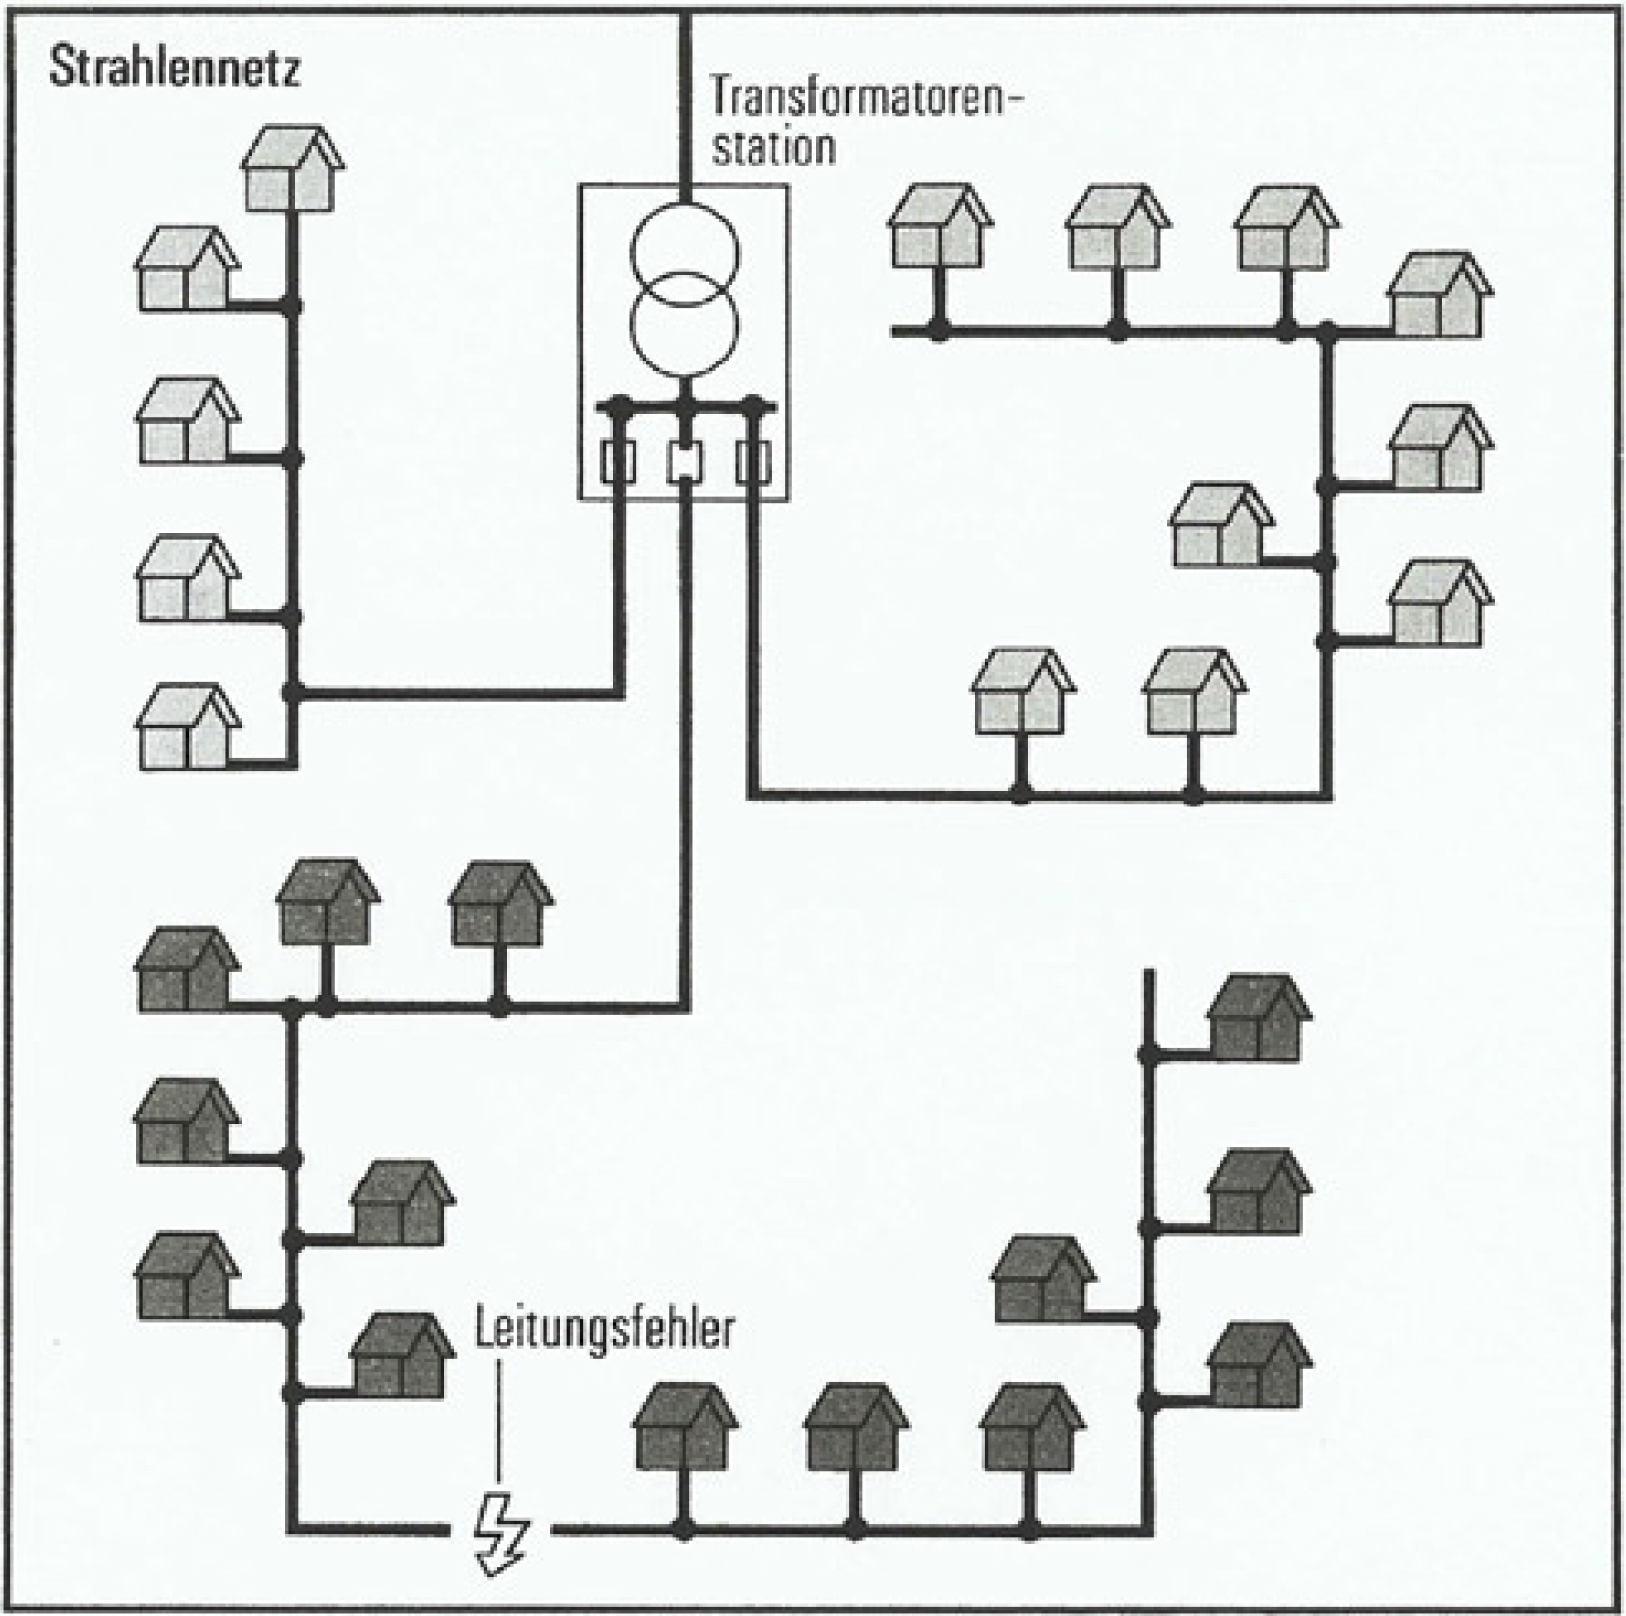
\includegraphics[width=0.9\textwidth]{images/Strahlnetz.png}
    \end{minipage}

% \textbf{Pro:}
%     \begin{itemize}
%         \item geringer Planungsaufwand
%         \item große Übersichtlichkeit bei der Fehlersuche
%         \item geringe Anforderungen an den Netzschutz
%     \end{itemize}
% \vspace{1em}
% \textbf{Contra:}
%     \begin{itemize}
%         \item größer werdende Spannungsabfälle mit zunehmendem Abstand von der Einspeisung
%         \item höhere Leistungsverluste mit zunehmendem Abstand von der Einspeisung
%     \end{itemize}

\subsection{Ringnetz}
    \begin{minipage}[t]{0.5\columnwidth}
        \begin{itemize}
            \pro höhere Versorgungssicherheit
            \pro geringere Verluste
            \pro verbesserte Spannungshaltung
            \vspace{1em}
            \con höhere Anspruch an die Qualifikation des Wartungspersonals
        \end{itemize}
    \end{minipage}%
    \hfill
    \begin{minipage}[t]{0.45\columnwidth}
        \centering \vspace{-0.7\baselineskip}
        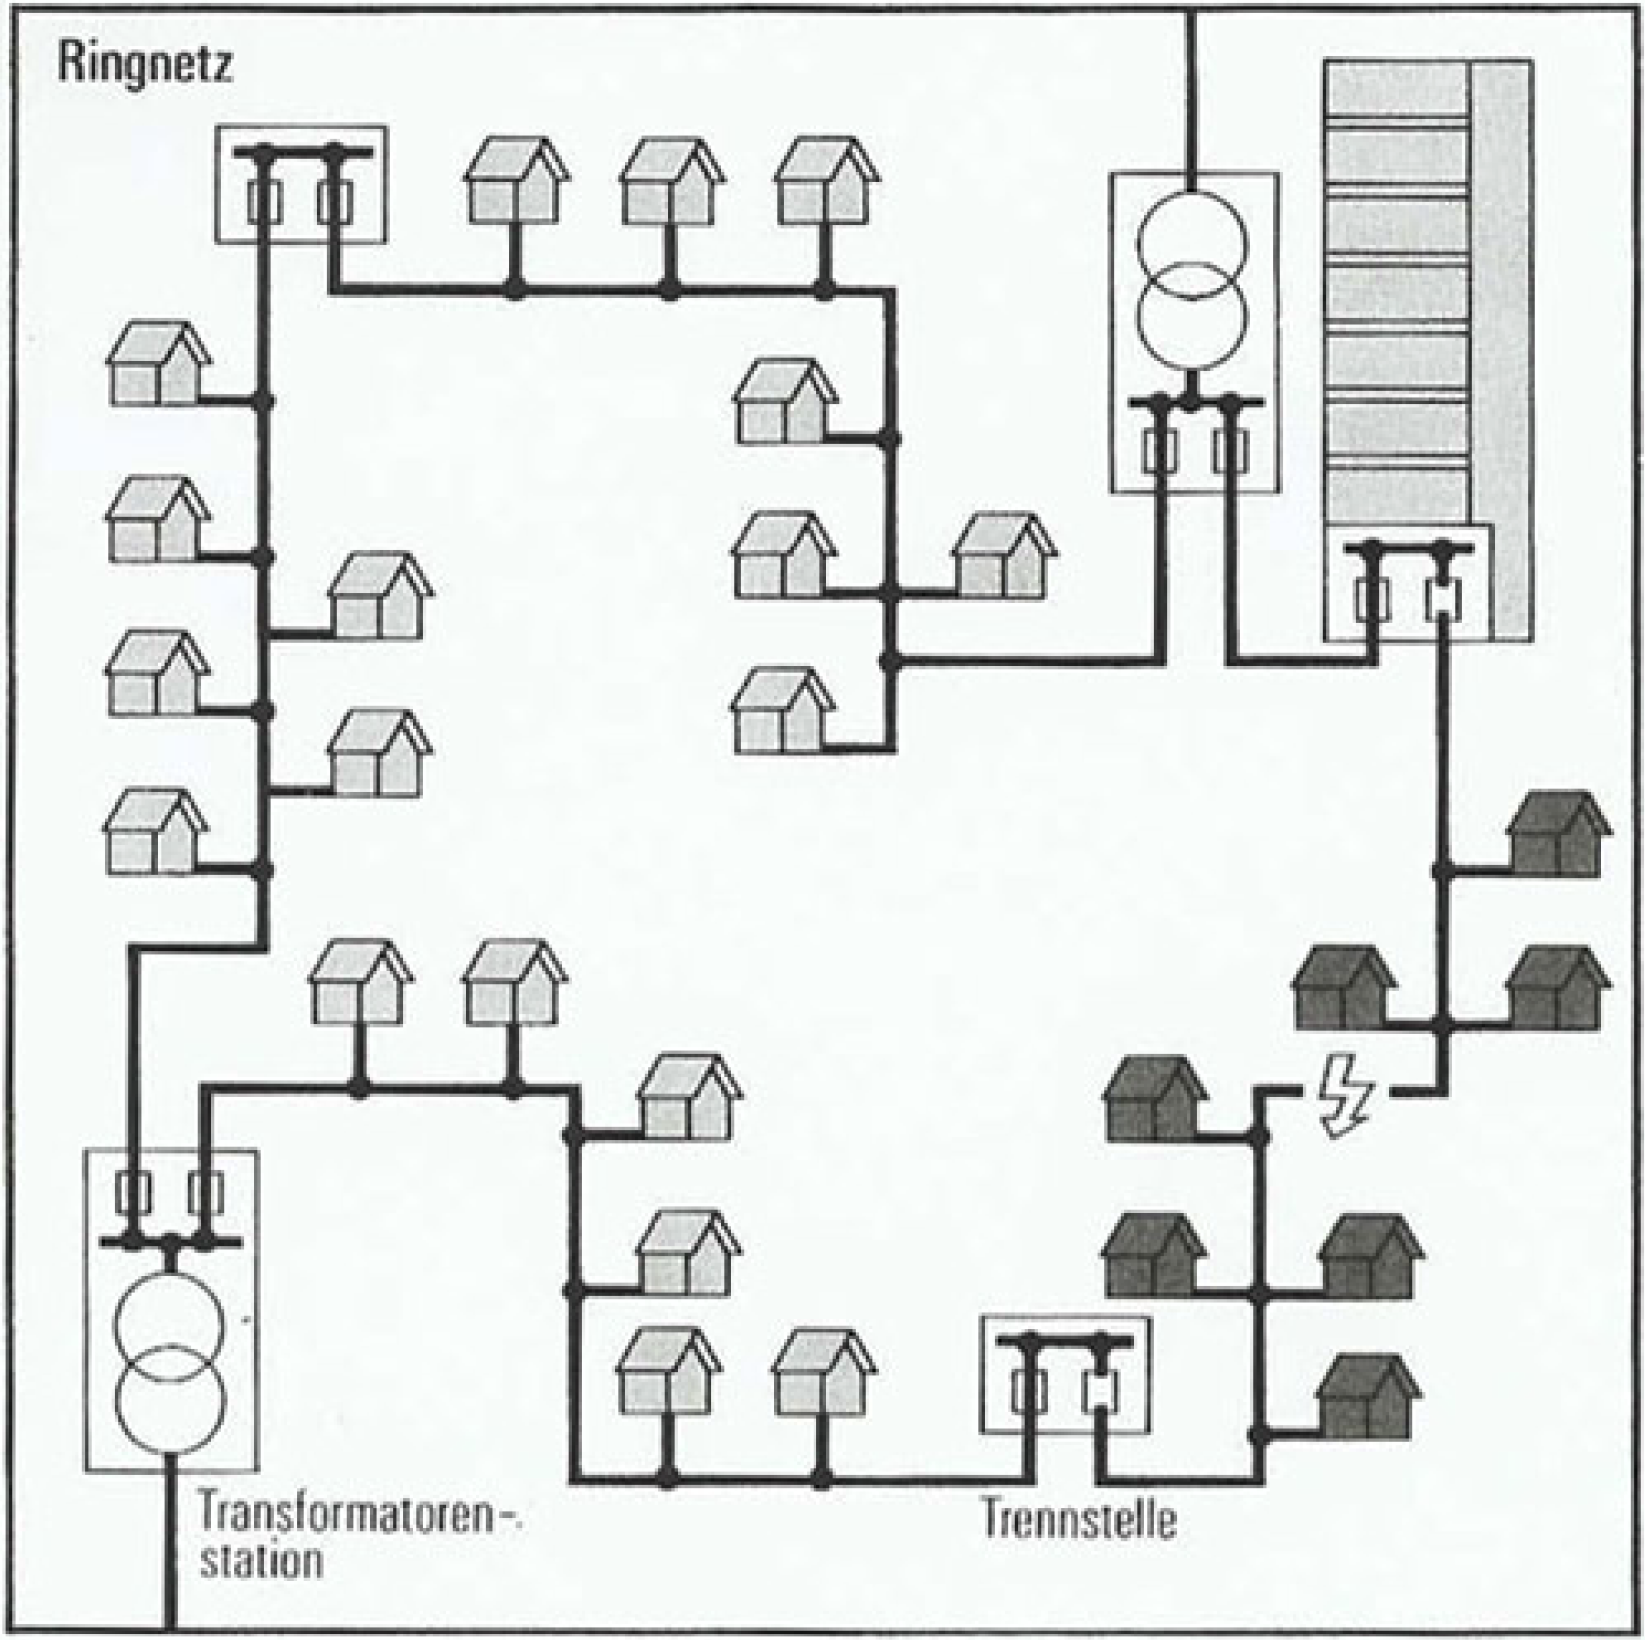
\includegraphics[width=0.9\textwidth]{images/Ringnetz.png}
    \end{minipage}

% 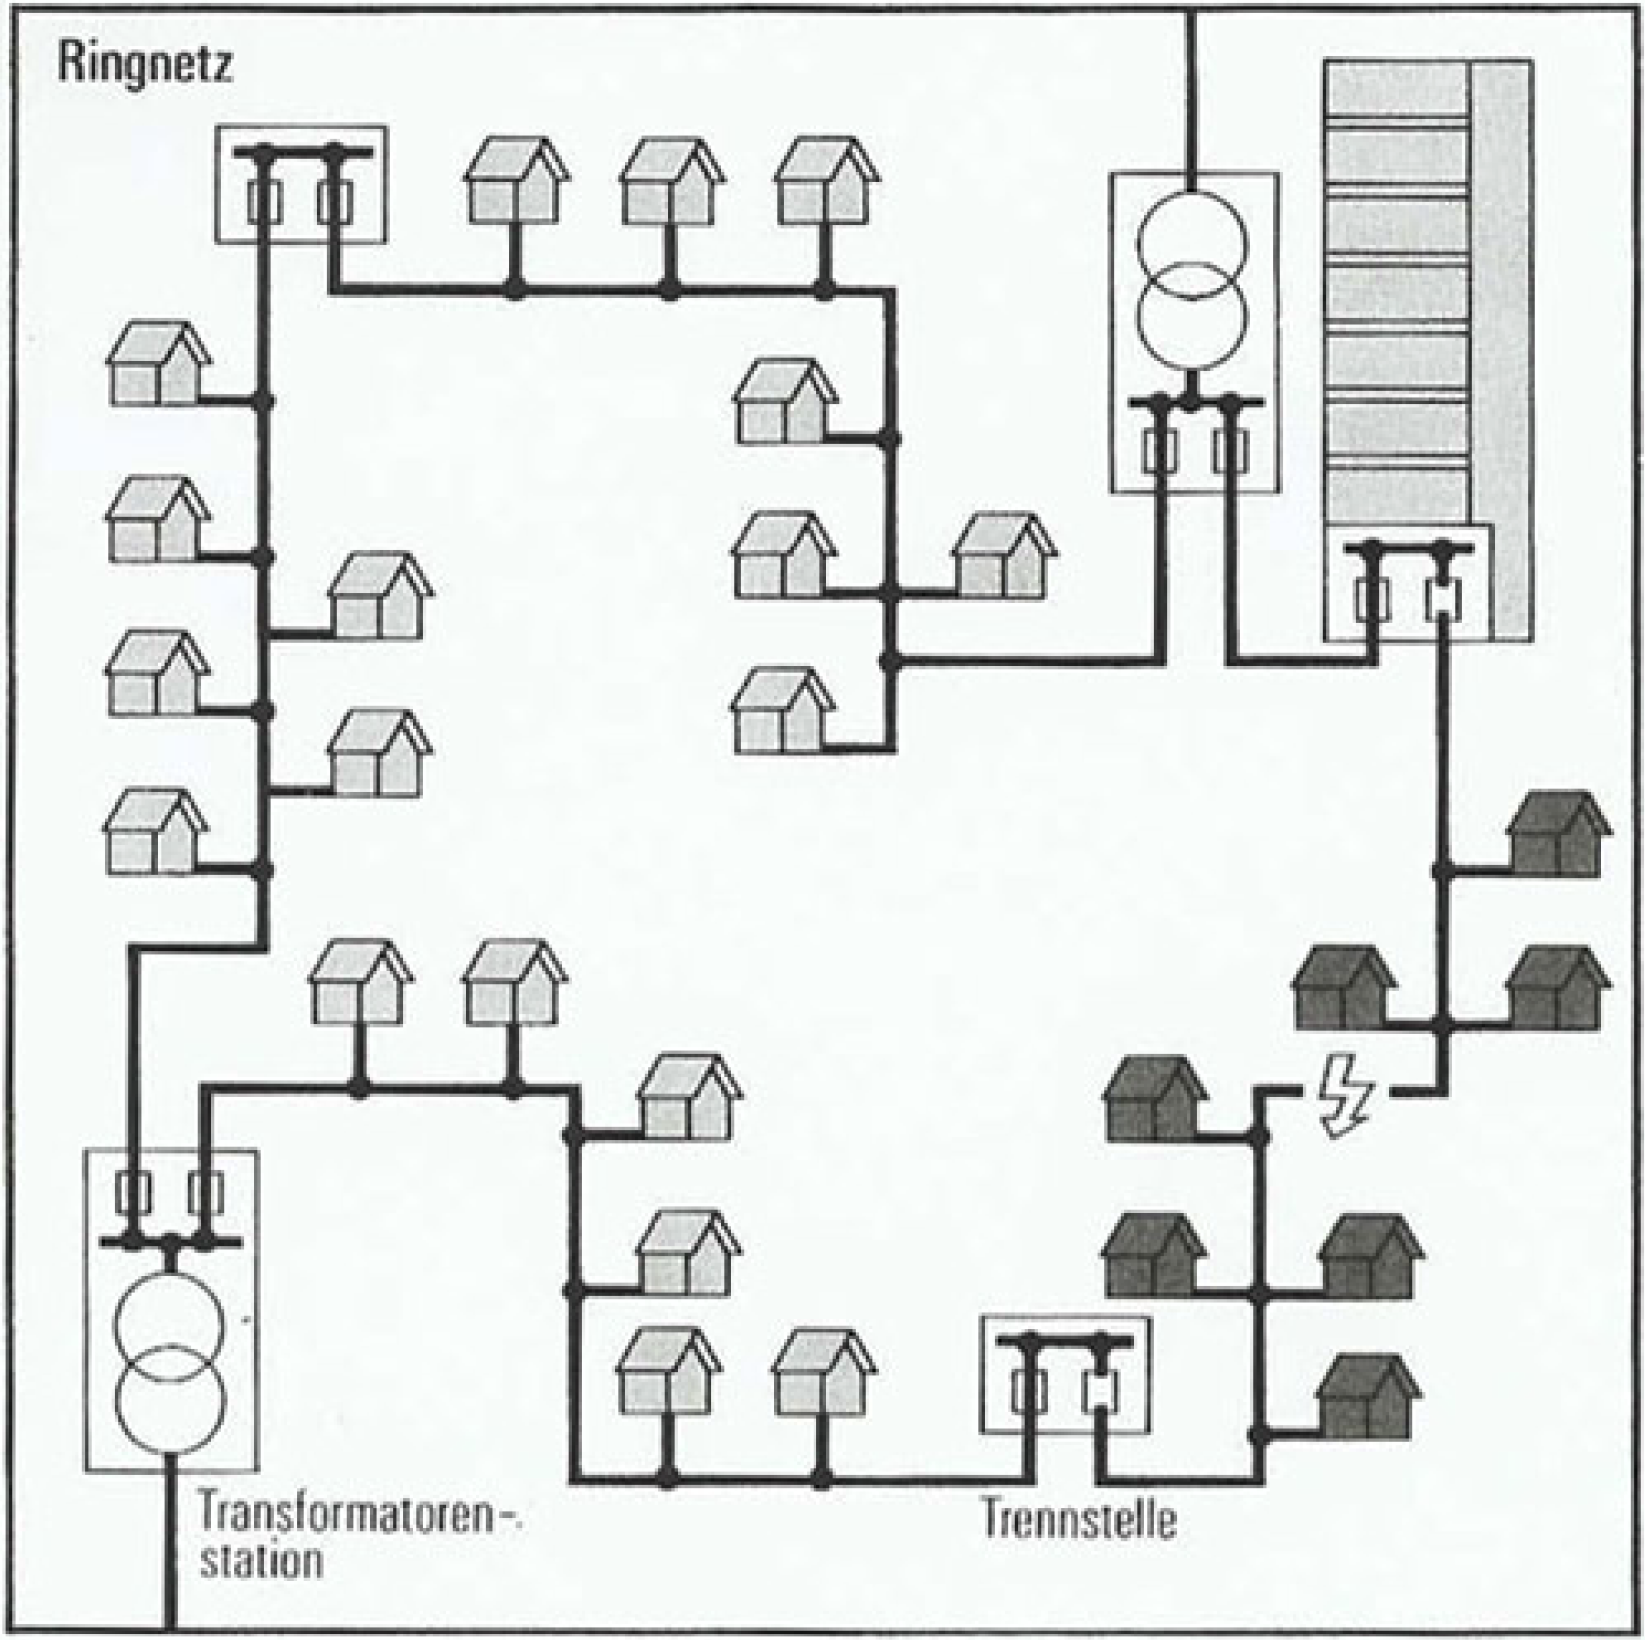
\includegraphics[width=0.55\columnwidth, align=c]{images/Ringnetz.png}

% \textbf{Pro:}
% \begin{itemize}
%     \item höhere Versorgungssicherheit
%     \item geringere Verluste
%     \item verbesserte Spannungshaltung
% \end{itemize}

% \vspace{1em}
% \textbf{Contra:}
% \begin{itemize}
%     \item höhere Anspruch an die Qualifikation des Wartungspersonals
% \end{itemize}

\subsection{Maschennetz}
    \begin{minipage}[t]{0.5\columnwidth}
        \begin{itemize}
            \pro eine optimale Versorgungszuverlässigkeit
            \pro optimale Spannungshaltung
            \pro minimale Leistungsverluste
        \vspace{1em}
            \con hohe Investitionskosten
            \con hohe Projektions- und Wartungsaufwand
            \con höhere Kurzschlussströme
        \end{itemize}
    \end{minipage}%
    \hfill
    \begin{minipage}[t]{0.45\columnwidth}
        \centering \vspace{-0.7\baselineskip}
        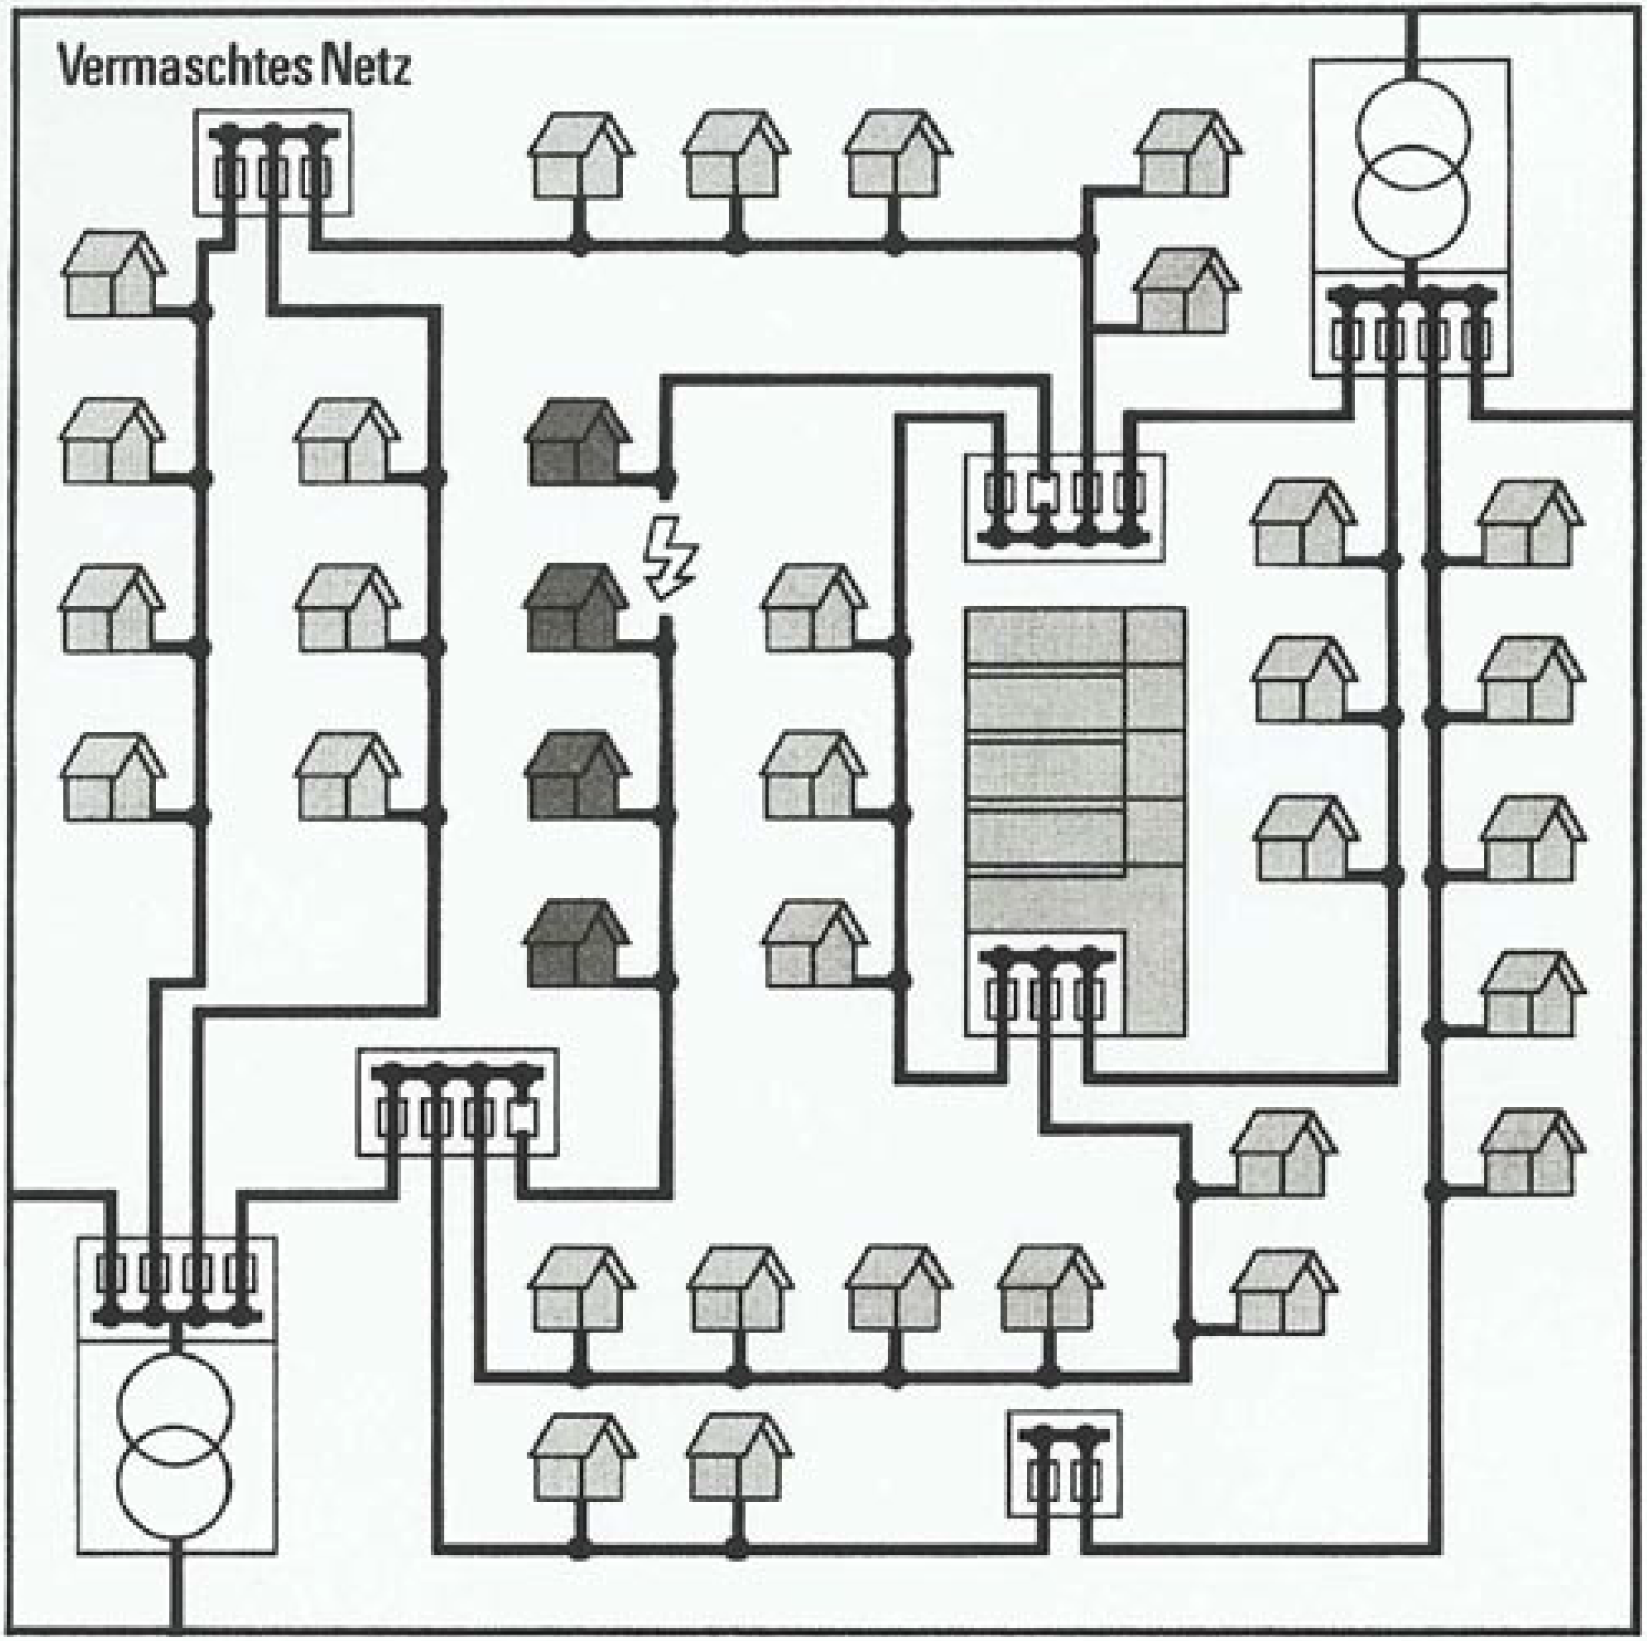
\includegraphics[width=0.9\textwidth]{images/Maschennetz.png}
    \end{minipage}

% 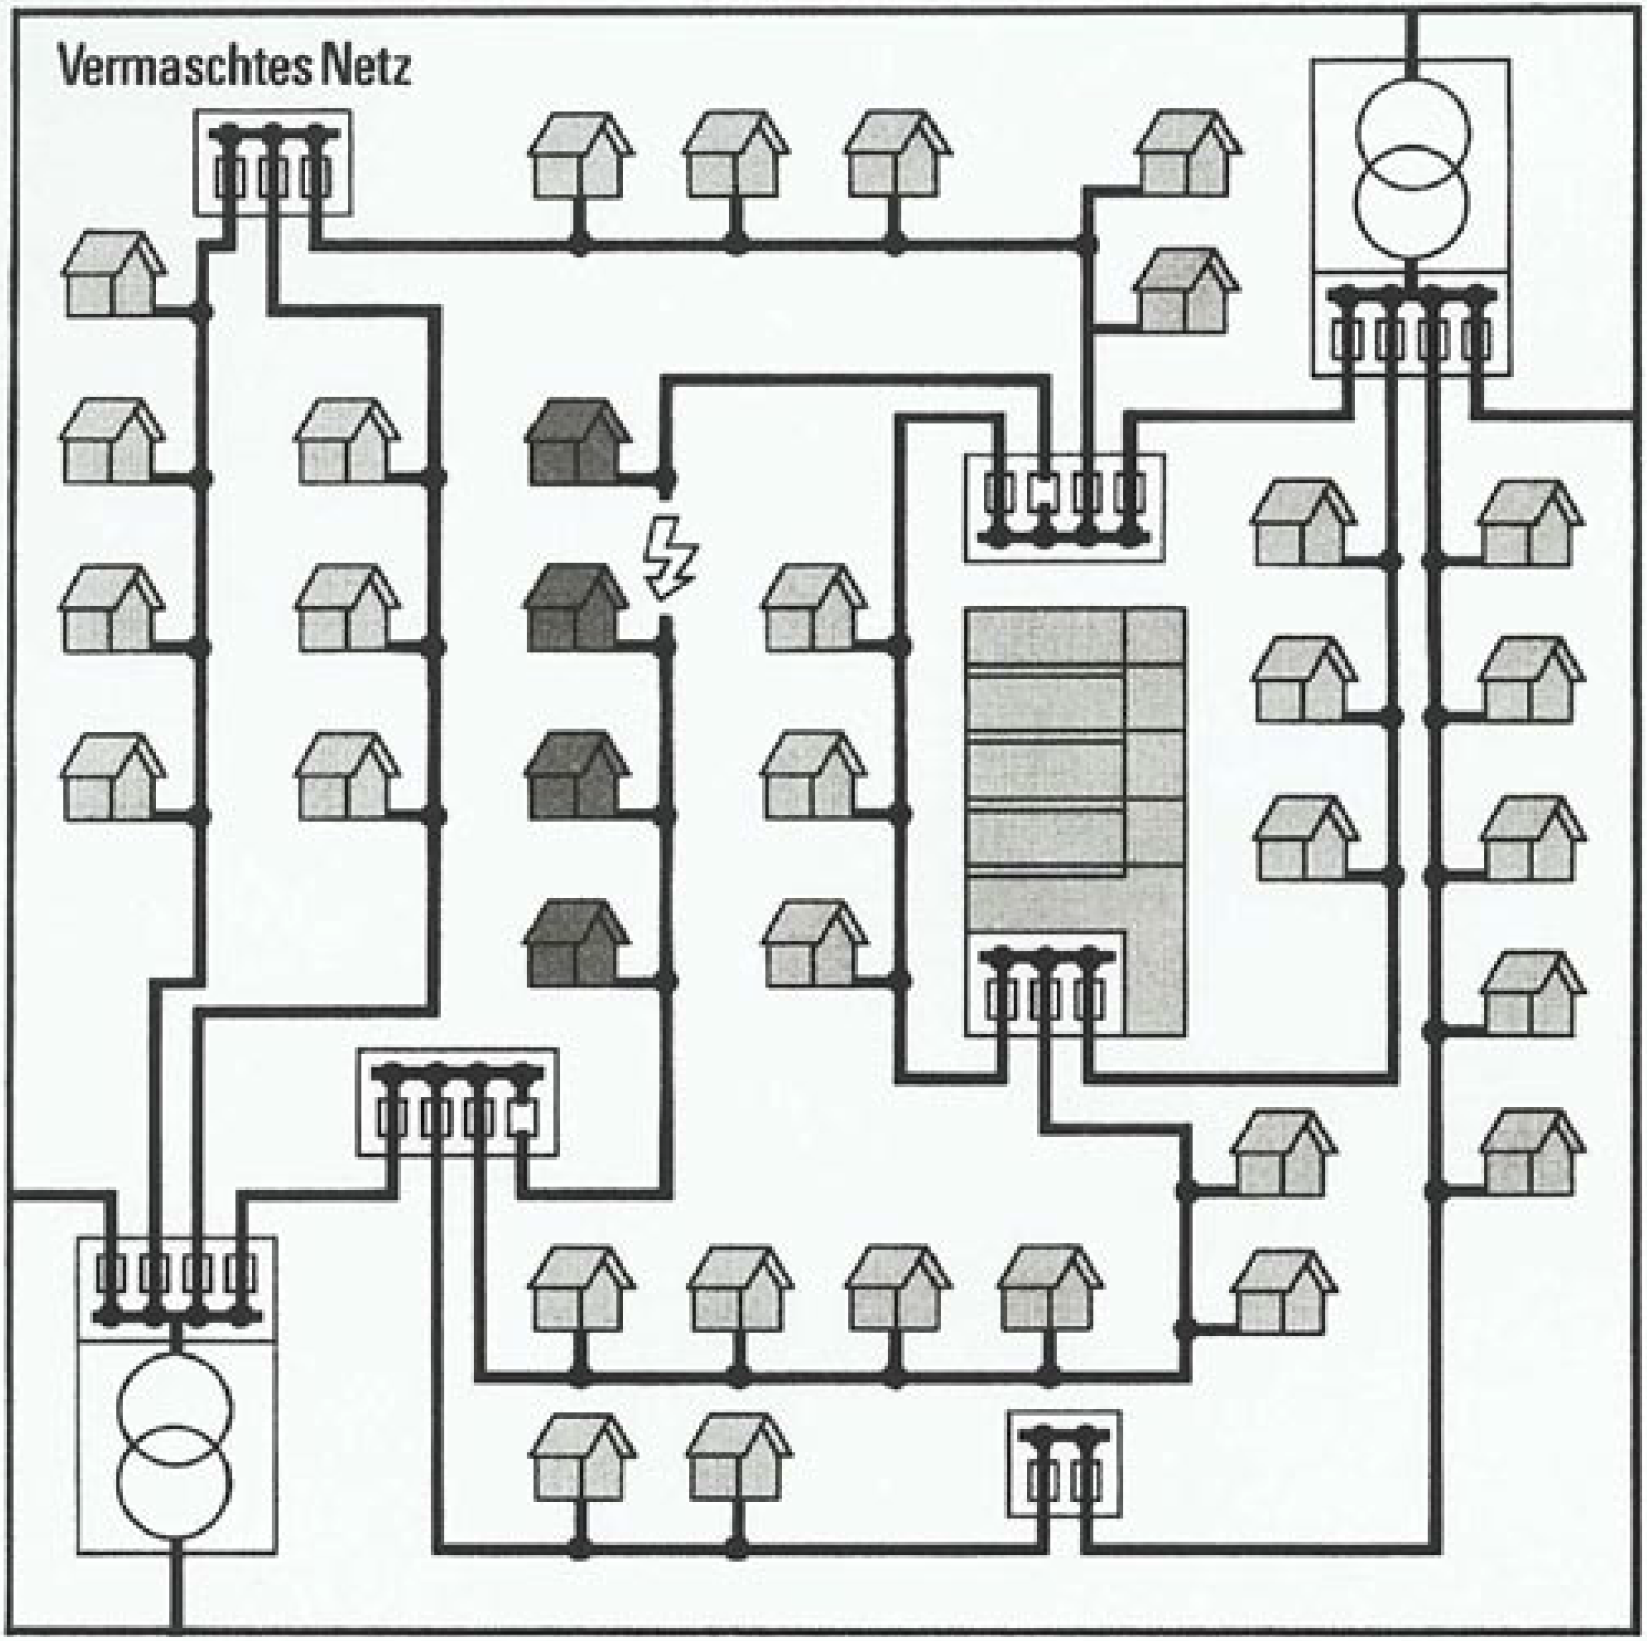
\includegraphics[width=0.55\columnwidth, align=c]{images/Maschennetz.png}

% \textbf{Pro:}
% \begin{itemize}
%     \item eine optimale Versorgungszuverlässigkeit
%     \item optimale Spannungshaltung
%     \item minimale Leistungsverluste
% \end{itemize}

% \vspace{1em}
% \textbf{Contra:}
% \begin{itemize}
%     \item hohe Investitionskosten
%     \item hohe Projektions- und Wartungsaufwand
%     \item höhere Kurzschlussströme
% \end{itemize} % done
        \section{Leitungen}
    % \textbf{Aufgabe:}
    % \begin{itemize}
    %     \item  Energieübertragung und -verteilung\\
    % \end{itemize}

    \textbf{Wichtigste Leitungsarten:}
    \begin{itemize}
        \item \textbf{Freileitungen} in praktisch allen Spannungsebenen
        \item \textbf{Kabelleitungen} mehr in den unteren Spannungsebenen
    \end{itemize}

\subsection{Freileitungen}
\subsubsection{Freileitungen: Vor- und Nachteile}
    % \textbf{Pro:}
    \begin{itemize}
        \pro günstige Investitionskosten
        \pro bessere Zugänglichkeit bei Reparaturen $\Rightarrow$ kürzere Wiederinbetriebnahmezeiten
    % \end{itemize}
    \vspace{1em}
    % \textbf{Contra:}
    % \begin{itemize}
        \con atmosphärischen Einwirkungen ausgesetzt
        \con Akzeptanzprobleme
    \end{itemize}

    \vspace{1em}
    \begin{itemize}
        \item \textbf{Material:}
        \begin{itemize}
            \item Al-Seile (99{,}5\% Al), Aldrey-Seile (> 98{,}5\% Al, Mg, Si, Fe) und Al-Stahl-Seile\\ 
            (Verhältnis Alu:Stahl typ. 6:1, z.\,B. 240/40 mm\textsuperscript{2}), Kupfer bei neuen Leitungen immer seltener
            \item Aluminium-Drähten $\Rightarrow$ eine gute elektrische Leitfähigkeit
            \item Stahlkern $\Rightarrow$ mechanische Festigkeit
            \item Aluminium gegenüber Kupfer deutlich günstiger
        \end{itemize}

        \item Ab 220\,kV $\Rightarrow$ Bündelleiter $\Rightarrow$ Sie führen also zur 
        \textbf{Verminderung des Wellenwiderstandes} und damit 
        \textbf{zur Erhöhung der übertragbaren Leistung.}

        \item \textbf{Hochtemperaturleiter:}
        \begin{itemize}
            \item normale Leiterseile $T_{\text{max}} = 80\,^{\circ}\mathrm{C}$
            \item Hochtemperaturseilen $T_{\text{max}} = 210\,^{\circ}\mathrm{C}$
            \item \textbf{Steigerung der Übertragungskapazität um bis zu 50 Prozent}
        \end{itemize}
    \end{itemize}

\subsubsection{Masten}
    \textbf{Funktionen:}
    \begin{itemize}
        \item \textbf{Tragmast:} Tragwerke für die Aufhängung der Leiter einer Freileitung
        \item \textbf{Abspannmasten:} Nehmen die Zugkräfte der Leiterseile an Winkelpunkten auf
        \item \textbf{Verdrillmast:} alle Aussenleiter eines Stromkreises auf dem Mast tauschen ihre Plätze\\
        (verbessertes Übertragungsverhalten).
    \end{itemize}

    \vspace{1em}
    \textbf{Materialien:}
    \begin{itemize}
        \item Stahl-Gittermast, Betonmast, Stahlrohrmast, Holzmast
    \end{itemize}

\subsubsection{Unterscheidungsmerkmale Freileitungen}
    \textbf{Die wichtigsten Unterscheidungsmerkmale:}
    \begin{itemize}
        \item Anzahl Phasen
        \item Länge der Isolatorenketten (Höhere Spannung $\Rightarrow$ längere Isolatorenketten)
        \item Abstand der Phasen und Höhe der Masten
    \end{itemize}

    \begin{minipage}[c]{0.48\columnwidth}
        \begin{center}
            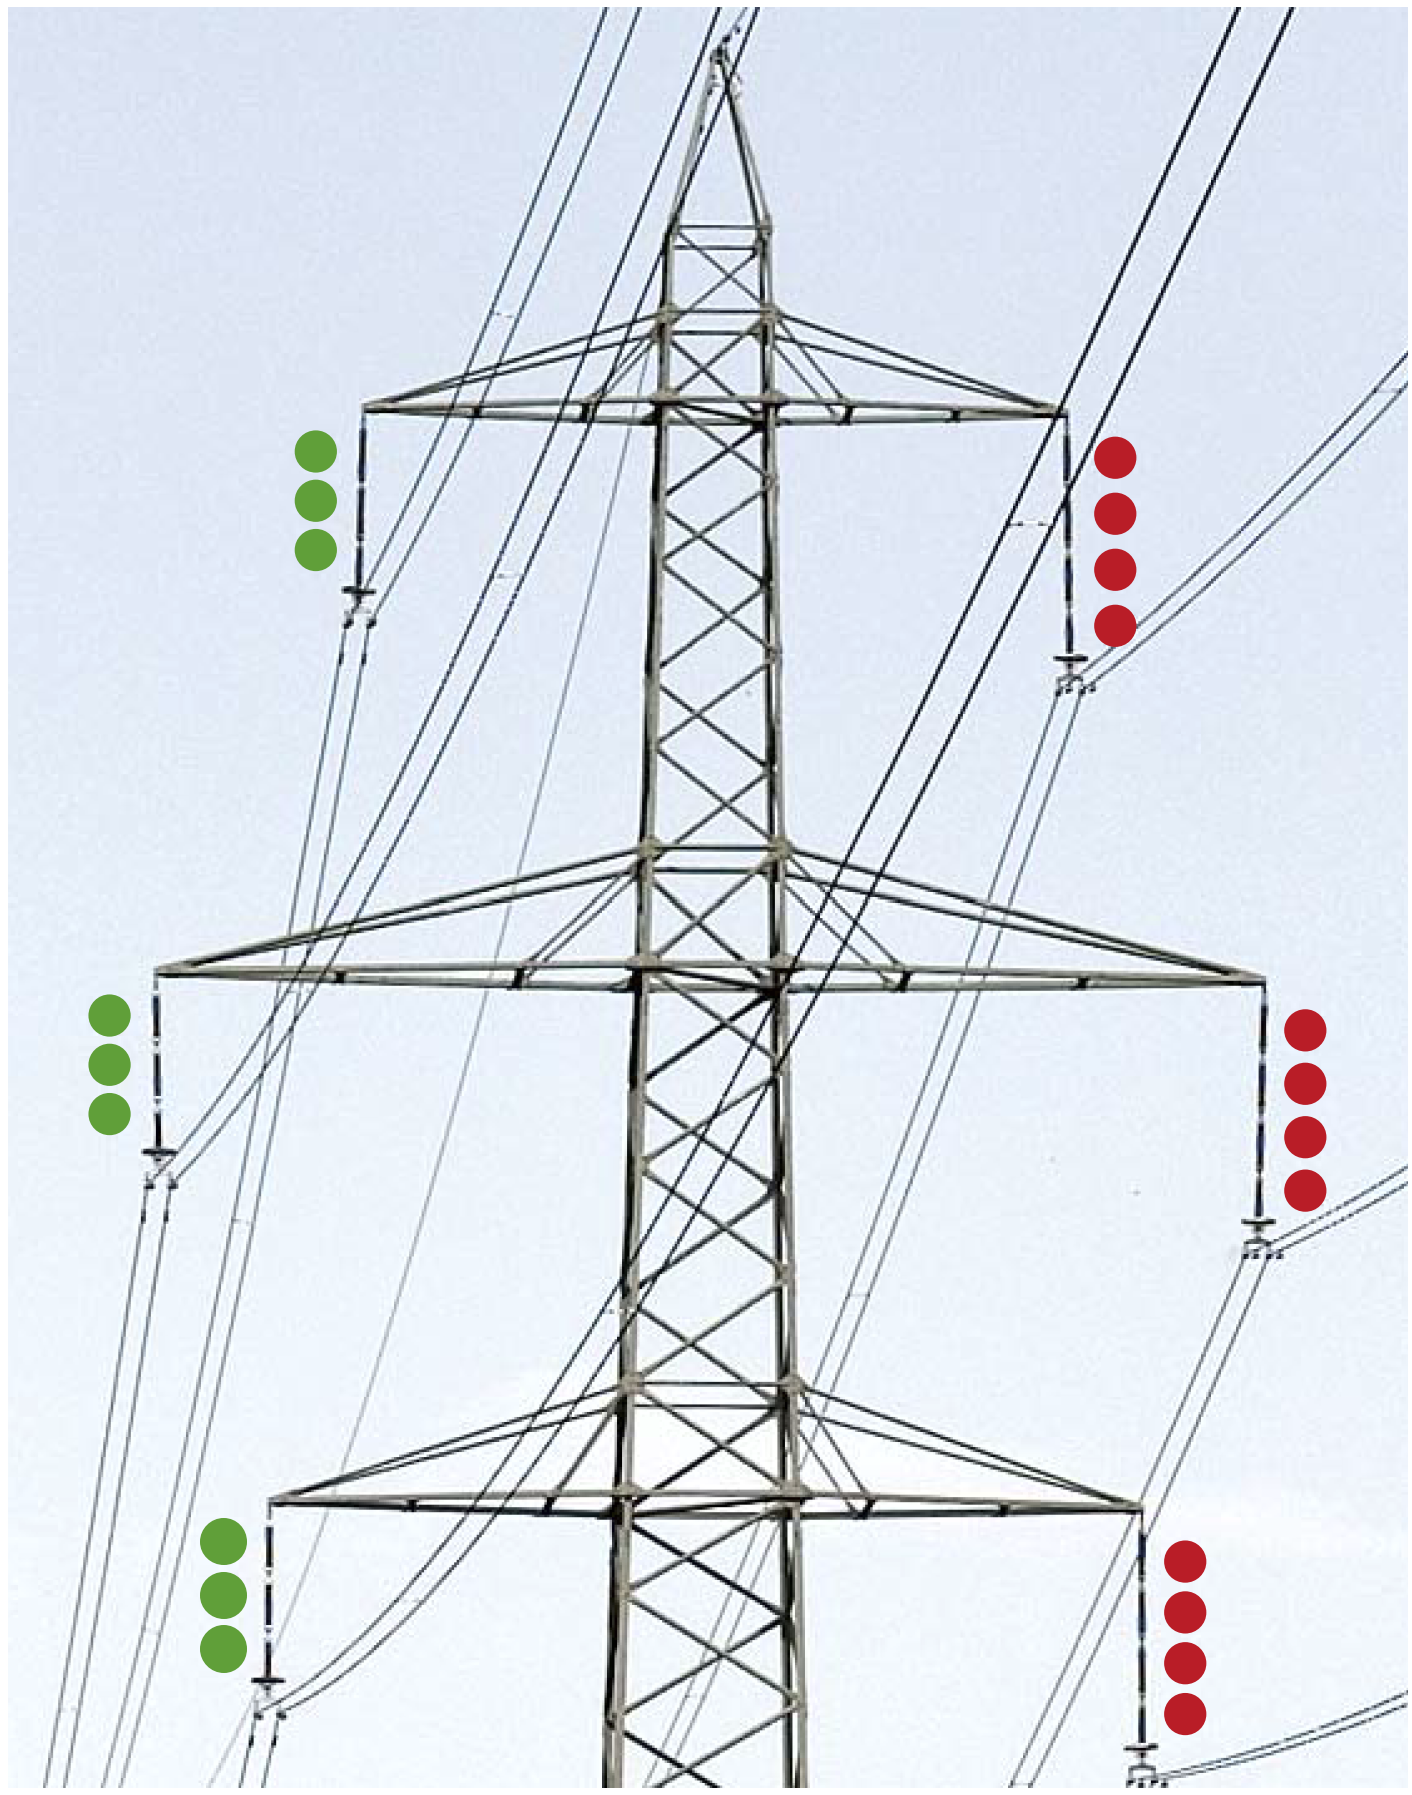
\includegraphics[width=0.9\textwidth, align=c]{images/Freileitungen_1.png}
        \end{center}
    \end{minipage}
    \hfill
    \begin{minipage}[c]{0.48\columnwidth}
        \begin{center}
            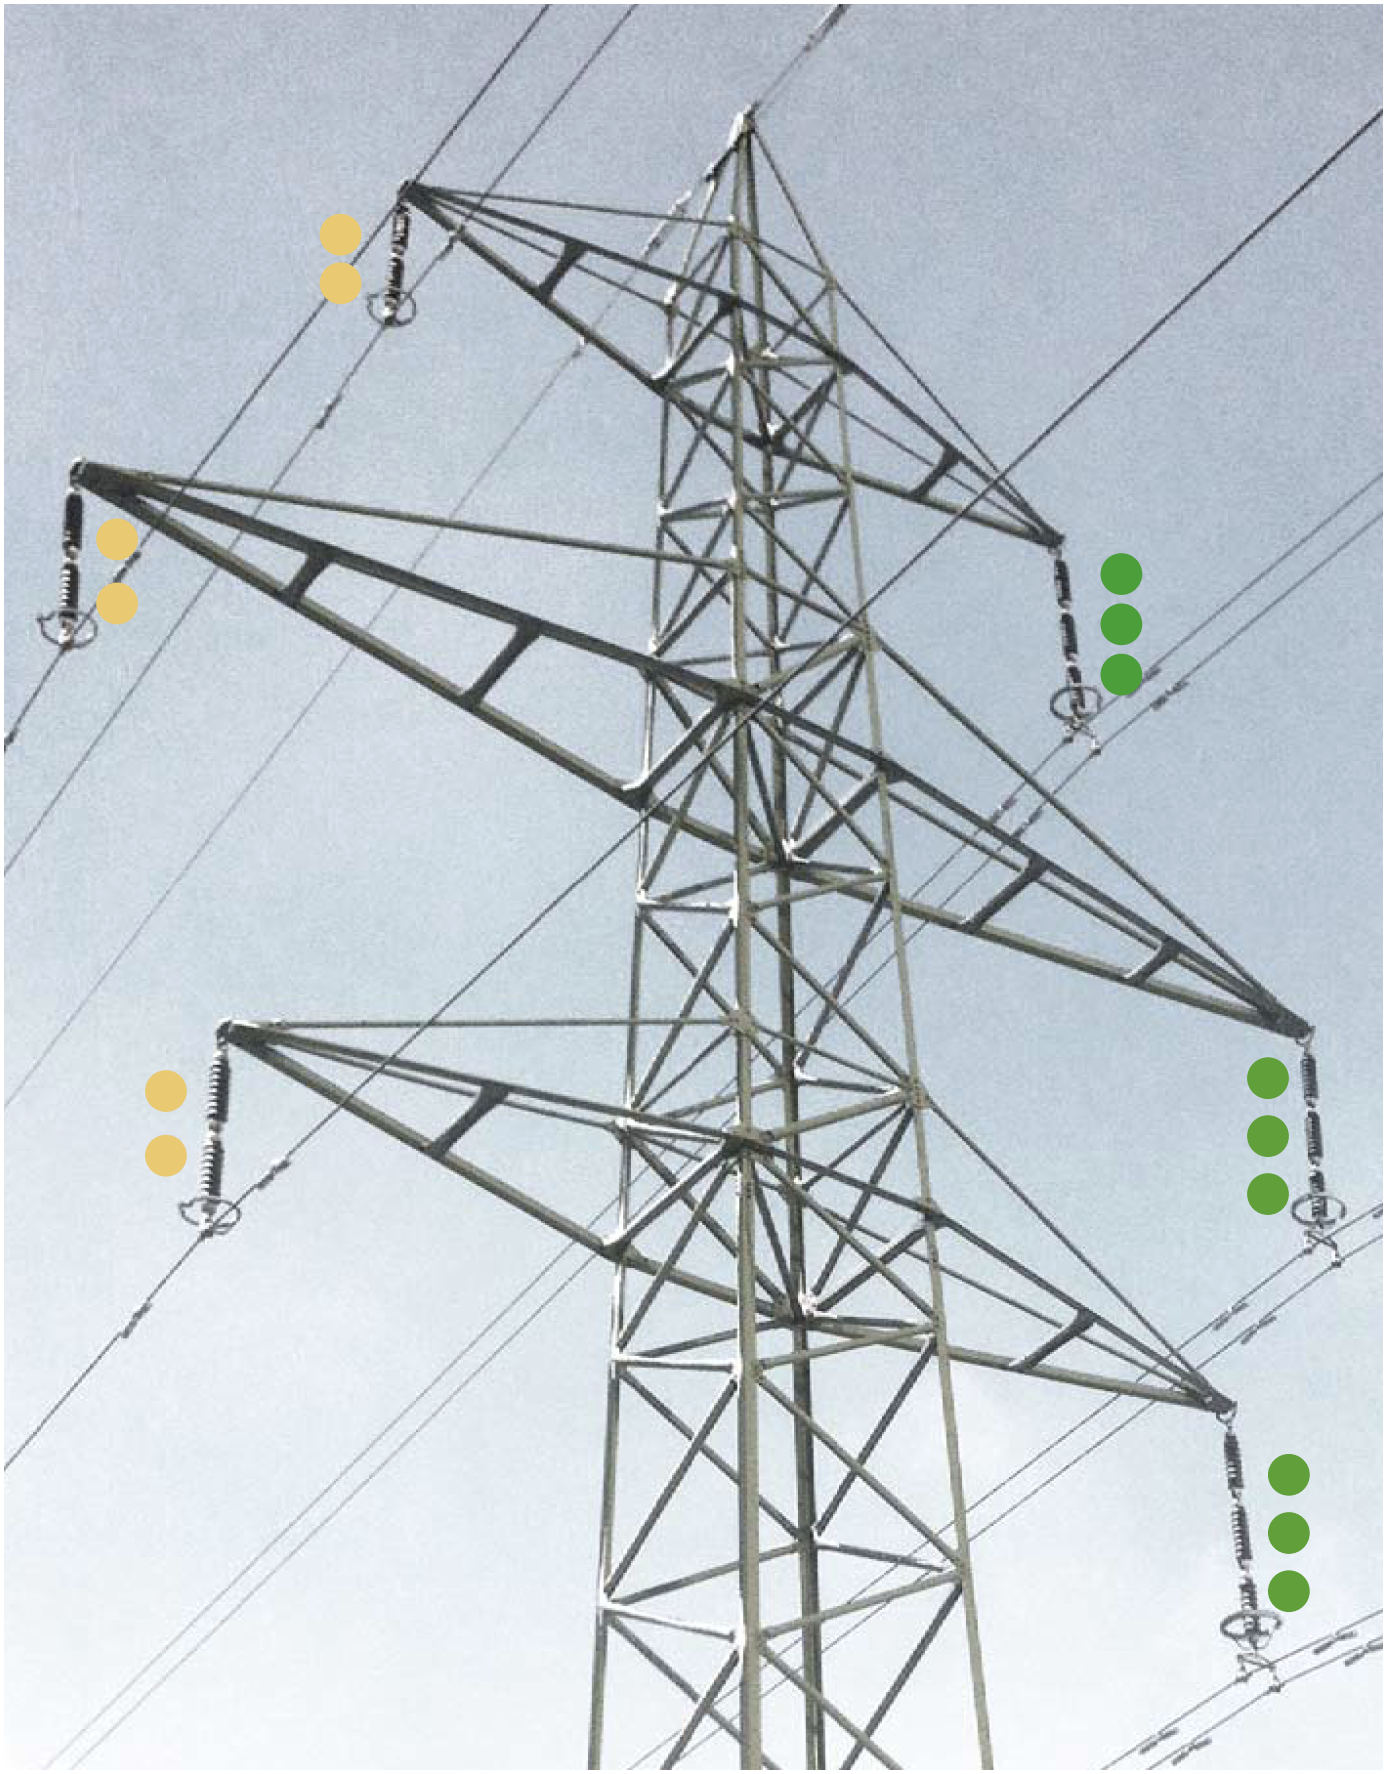
\includegraphics[width=0.9\textwidth, align=c]{images/Freileitungen_2.png}
        \end{center}
    \end{minipage}
% \newcolumn

\subsubsection{Mastenformen}
    \begin{multicols}{3}
        \textbf{Donaumast}

        Zwei Drehstromkreise, bei denen die Leiter jeweils im Dreieck angeordnet sind

        \begin{center}
            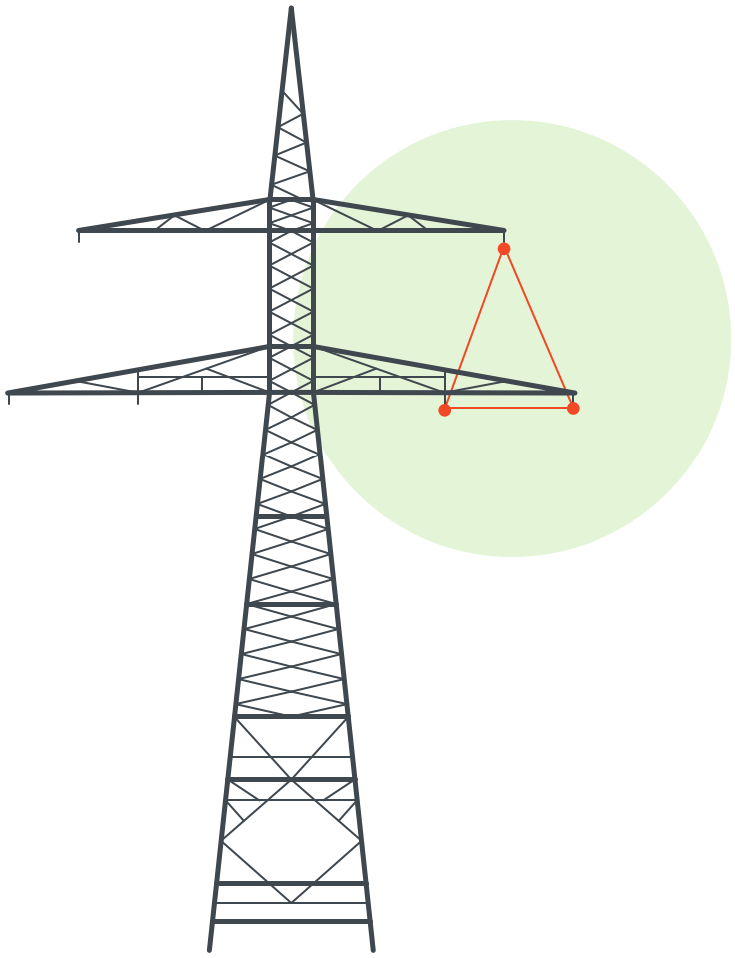
\includegraphics[width=0.8\columnwidth, align=b]{images/Mastenformen_1.png}
        \end{center}

        \vfill
        \columnbreak

        \textbf{Einebenenmast}

        Niedrige Bauhöhe und grössere Trassenbreite

        \begin{center}
            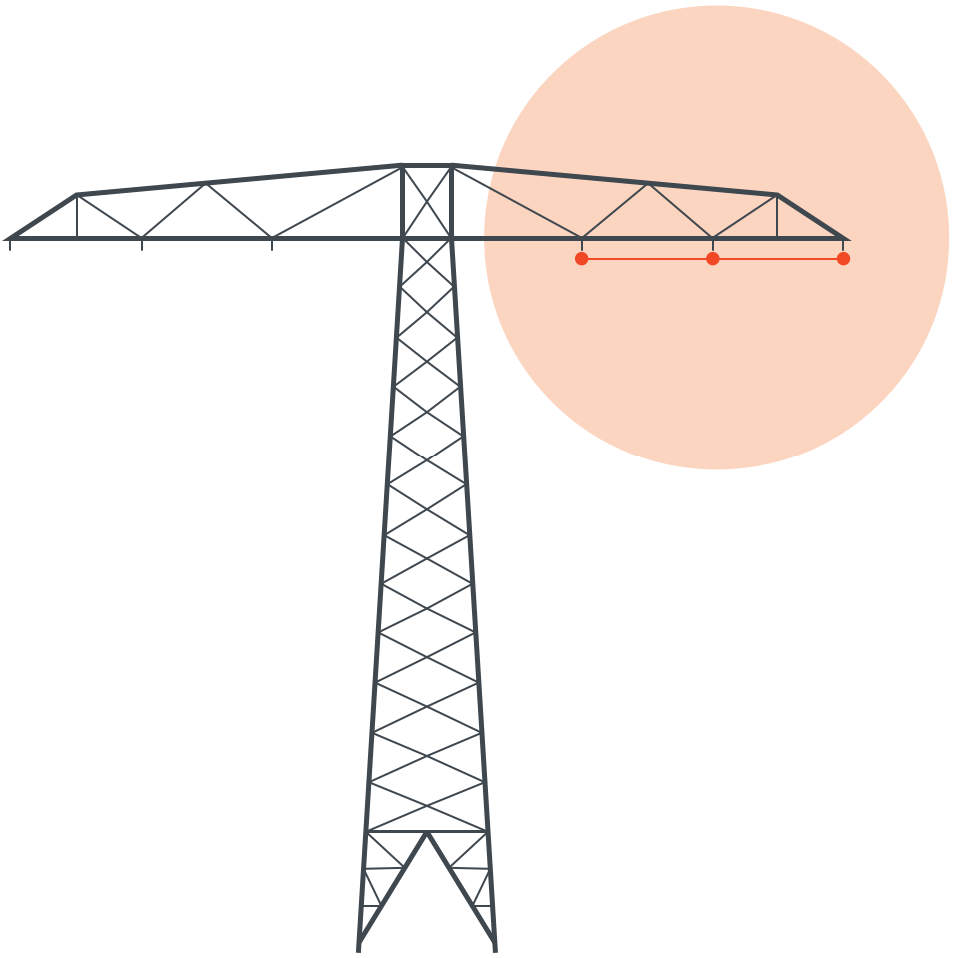
\includegraphics[width=0.8\columnwidth, align=b]{images/Mastenformen_2.png}
        \end{center}

        \vfill
        \columnbreak

        \textbf{Tonnenmast}

        Geringe Trassenbreite, aber höher als vergleichbare Donaumasten

        \begin{center}
            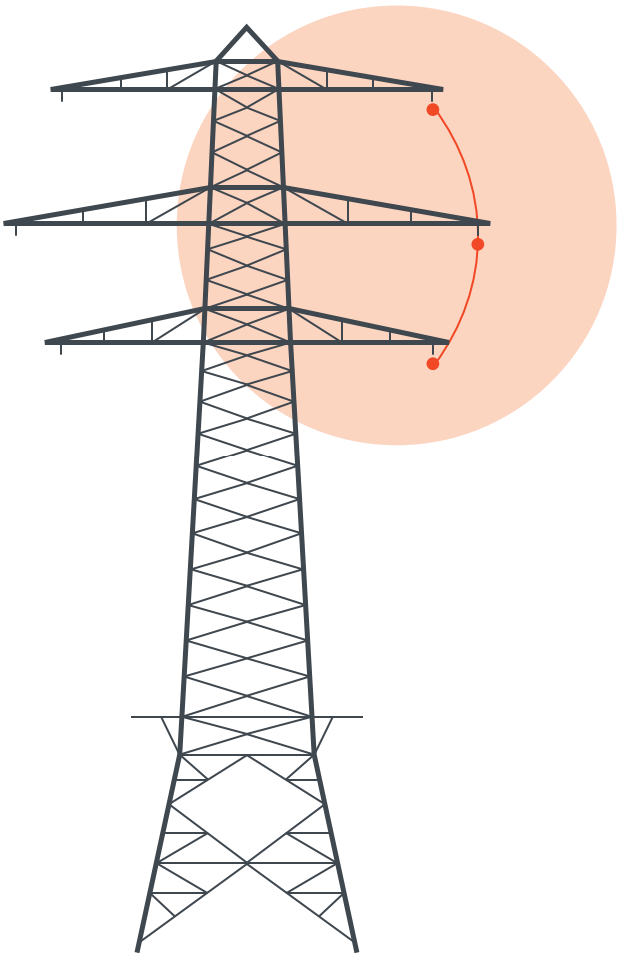
\includegraphics[width=0.8\columnwidth, align=b]{images/Mastenformen_3.png}
        \end{center}
    \end{multicols}
%     \begin{minipage}[c]{0.4\columnwidth}
%         \textbf{Donaumast}
%     \end{minipage}
%     \hfill
%     \begin{minipage}[c]{0.56\columnwidth}
%         \textbf{Einebenenmast}
%     \end{minipage}
%     \begin{minipage}[c]{0.4\columnwidth}
%         Zwei Drehstromkreise bei denen die Leiter jeweils im Dreieck angeordnet sind
%     \end{minipage}
%     \hfill
%     \begin{minipage}[c]{0.56\columnwidth}
%         Niedrigen Bauhöhe und eine grössere Trassenbreite
%     \end{minipage}

%     \begin{minipage}[c]{0.4\columnwidth}
%         \begin{center}
%             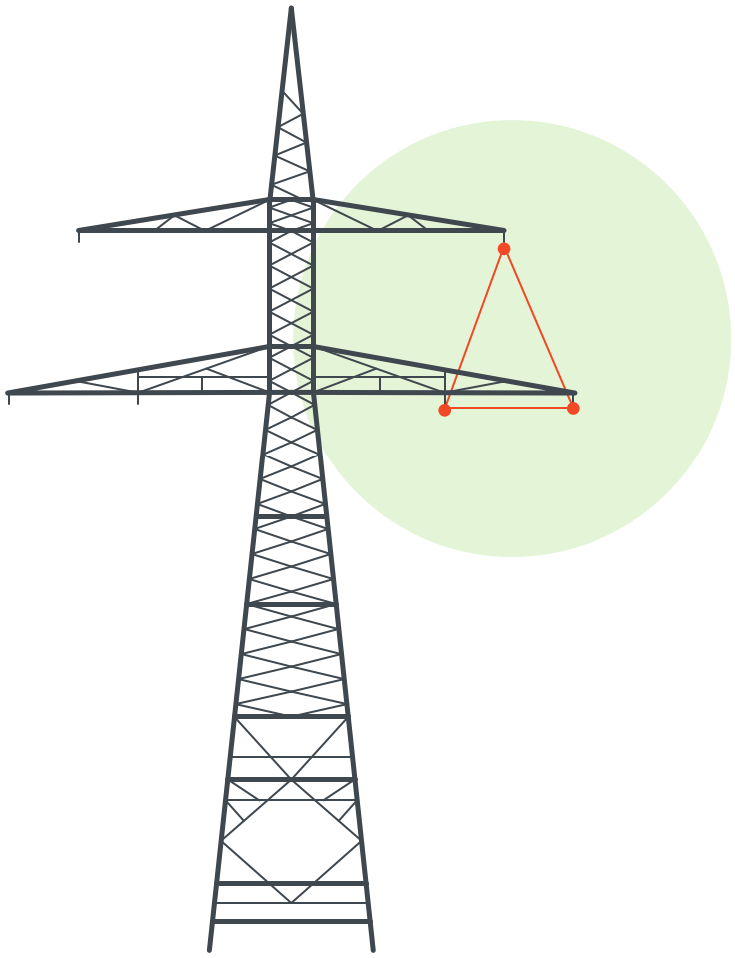
\includegraphics[height=5cm, align=c]{images/Mastenformen_1.png}
%         \end{center}
%     \end{minipage}
%     \hfill
%     \begin{minipage}[c]{0.56\columnwidth}
%         \begin{center}
%             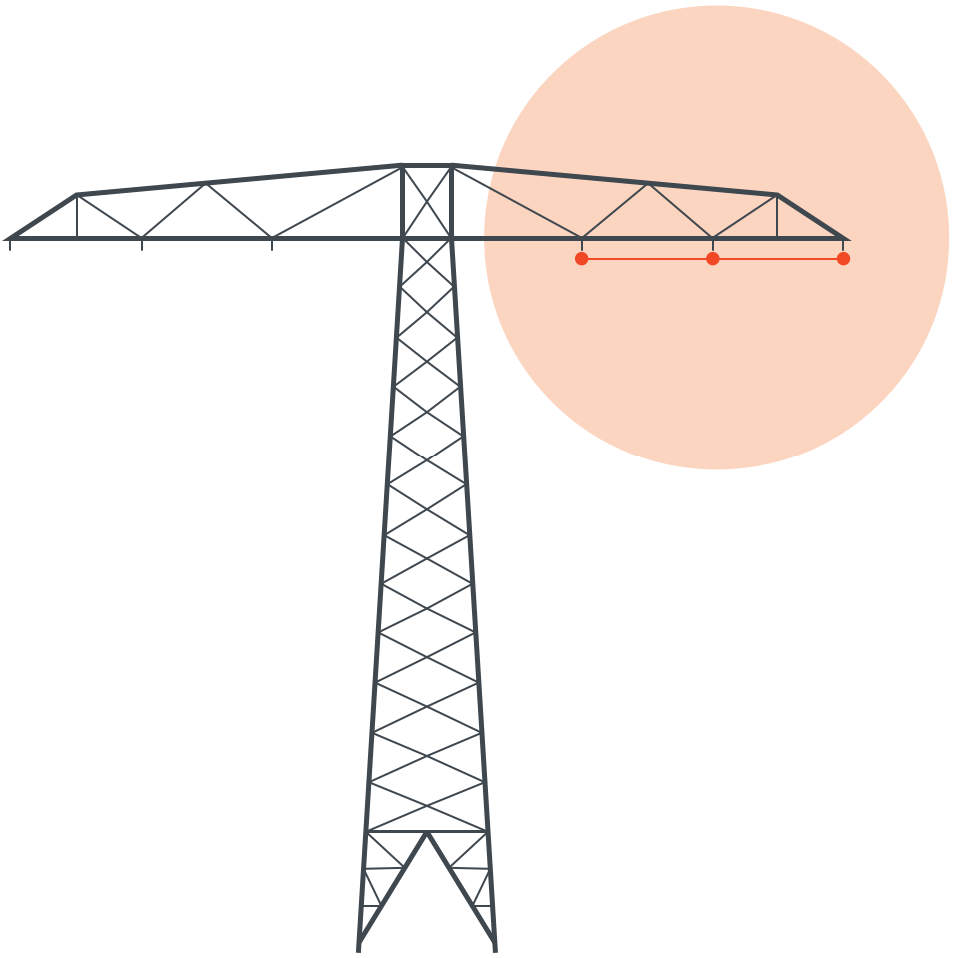
\includegraphics[height=5cm, align=c]{images/Mastenformen_2.png}
%         \end{center}
%     \end{minipage}

% \vspace{0.25cm}

%     \begin{minipage}[c]{0.5\columnwidth}
%         \textbf{Tonnenmast}\\
%         Eine geringe Trassenbreite, sind aber höher als vergleichbare Donaumasten

%         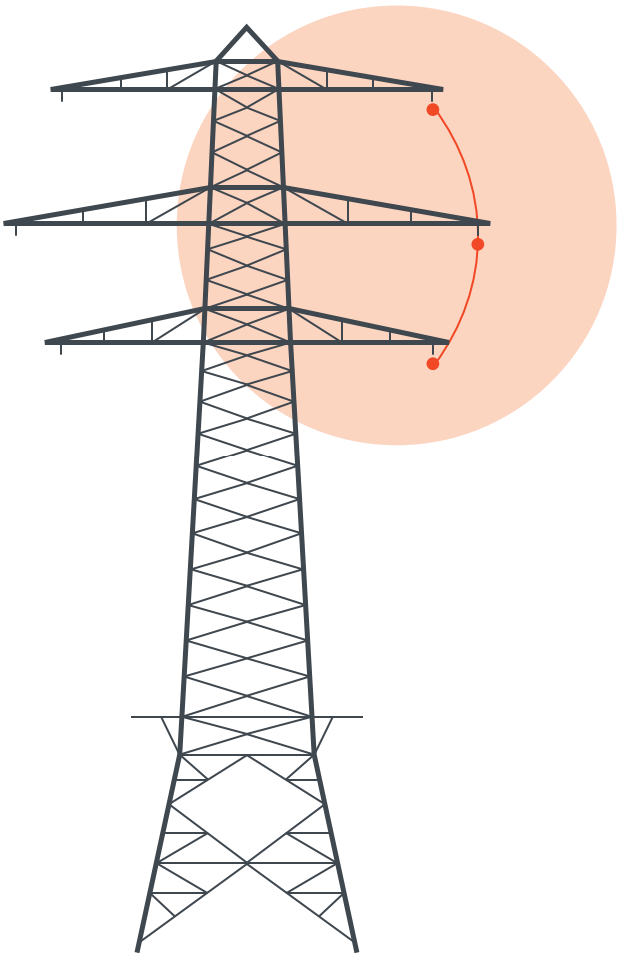
\includegraphics[height=5cm, align=c]{images/Mastenformen_3.png}    
%     \end{minipage}

\subsection{Kabelleitungen}
\subsubsection{Material}
    \begin{tabular}{>{\bfseries}l l}
        Leiter: & Kupfer oder Aluminium \\
        Isolierung: & öl-imprägniertes Papier oder Kunststoffe wie Polyäthylen (PE), \\
                    & vernetztes Polyäthylen (VPE) sowie Polyvinylchlorid (PVC) \\
        Schutzmantel: & Metall \\
    \end{tabular}

\subsubsection{Aufbau}
    \begin{center}
        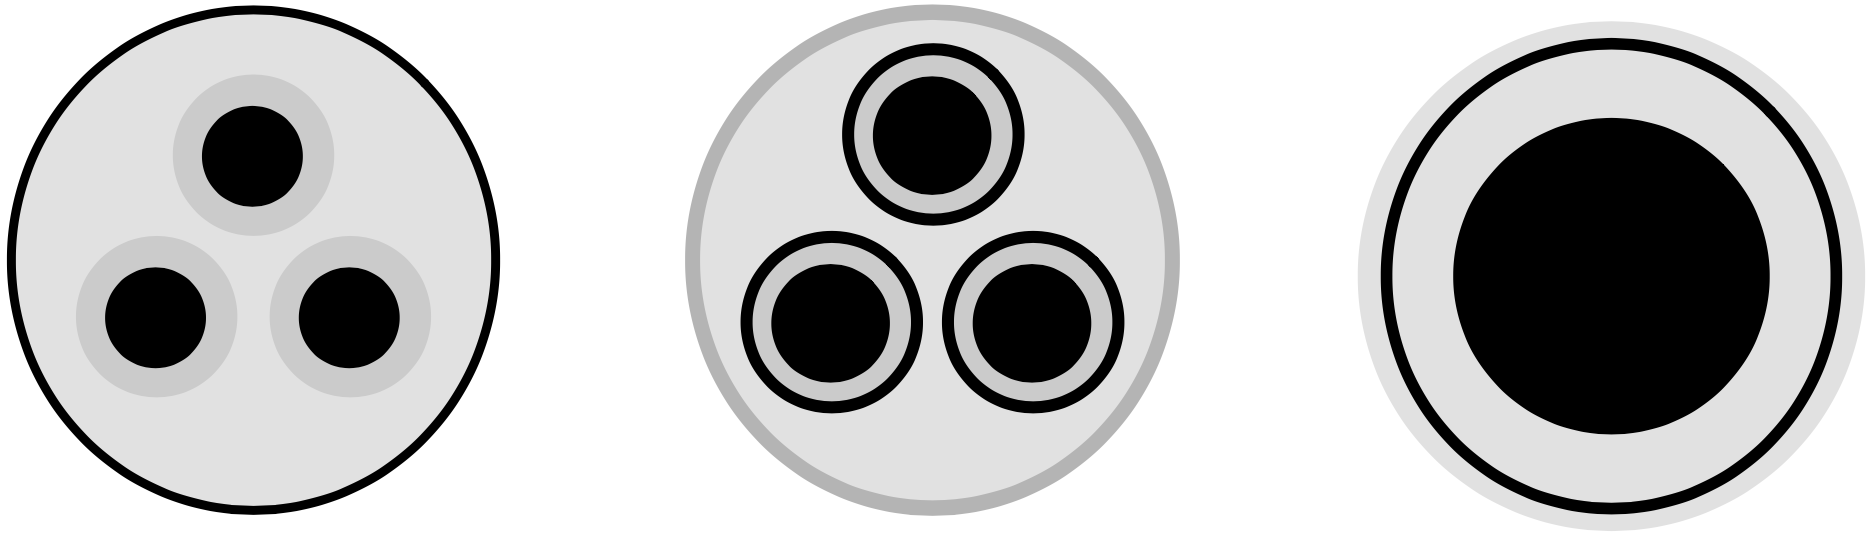
\includegraphics[width=0.8\linewidth]{images/Kabelaufbau.png}
    \end{center}
    \begin{multicols}{3}
        \textbf{Gürtelkabel:}\\
        Nichtradiales elektrisches Feld, Verwendung im Nieder- und Mittelspannungsbereich
        \vfill
        \columnbreak
        \textbf{Dreimantel-Kabel:}\\
        Radiales elektrisches Feld, Verwendung im Nieder- und Mittelspannungsbereich
        \vfill\null
        \columnbreak
        \textbf{Einleiterkabel:}\\
        Radiales elektrisches Feld, Verwendung im oberen Mittelspannungs- und im Hochpannungsbereich
    \end{multicols}

\subsubsection{Kabel: Vor- und Nachteile}
    % \textbf{Pro:}
    \begin{itemize}
        \pro geschützt vor atmosphärischen Einwirkungen $\Rightarrow$ kleinere Ausfallsrate
        \pro bessere Akzeptanz
    % \end{itemize}
    \vspace{1em}
    % \textbf{Contra:}
    % \begin{itemize}
        \con schwierigere Zugänglichkeit bei Reparaturen $\Rightarrow$ längere Wiederinbetriebnahmezeiten
        \con im Hochspannungsbereich teurer (wirtschaftlich nur für kurze Strecken)
    \end{itemize}

\subsubsection{Erdverkabelung in der Schweiz}
    \textbf{Erdverkabelung pro Netzebene in der Schweiz}\\
    \begin{tabular}{>{\bfseries}l r >{\bfseries}l r}
        Netzebene 1 & 8 km      & Netzebene 5 & 30'607 km \\
        Netzebene 3 & 1'893 km  & Netzebene 7 & 72'852 km \\
    \end{tabular}

% \newcolumn % done
        \input{sections/54_Komponenten_und_Technologie_Schaltanlagen_Umspanwerke.tex} % done
        \section{Leitungsbeläge}

\subsection{Elektrisches und magnetisches Feld}
% 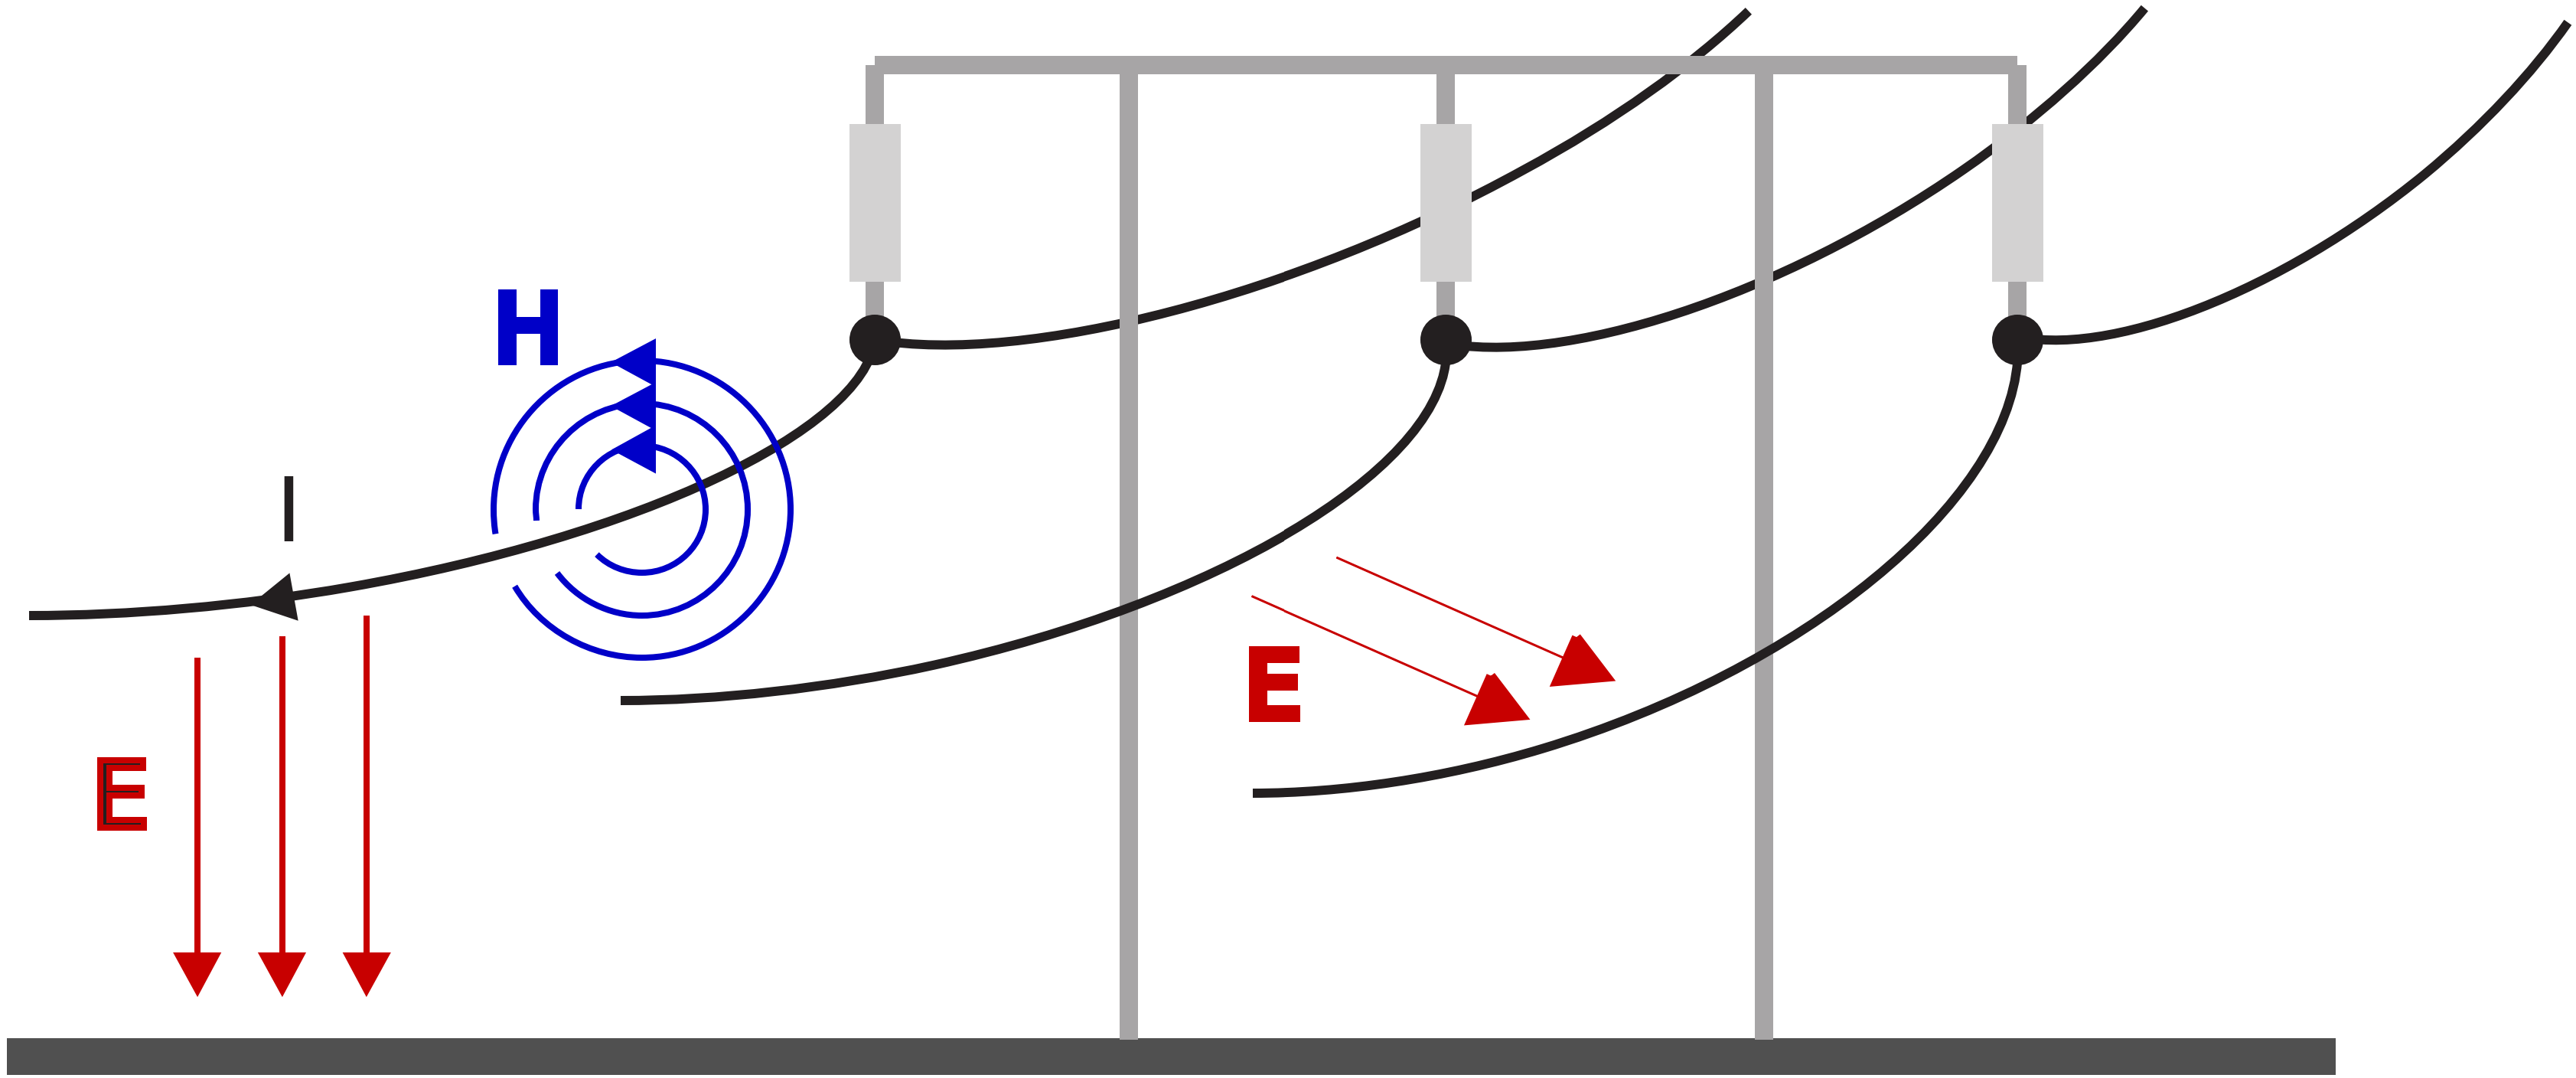
\includegraphics[width=0.98\columnwidth, align=c]{images/Elektrisches_und_Magnetisches_Feld.png}

\subsubsection{Ersatzschaltbild}
    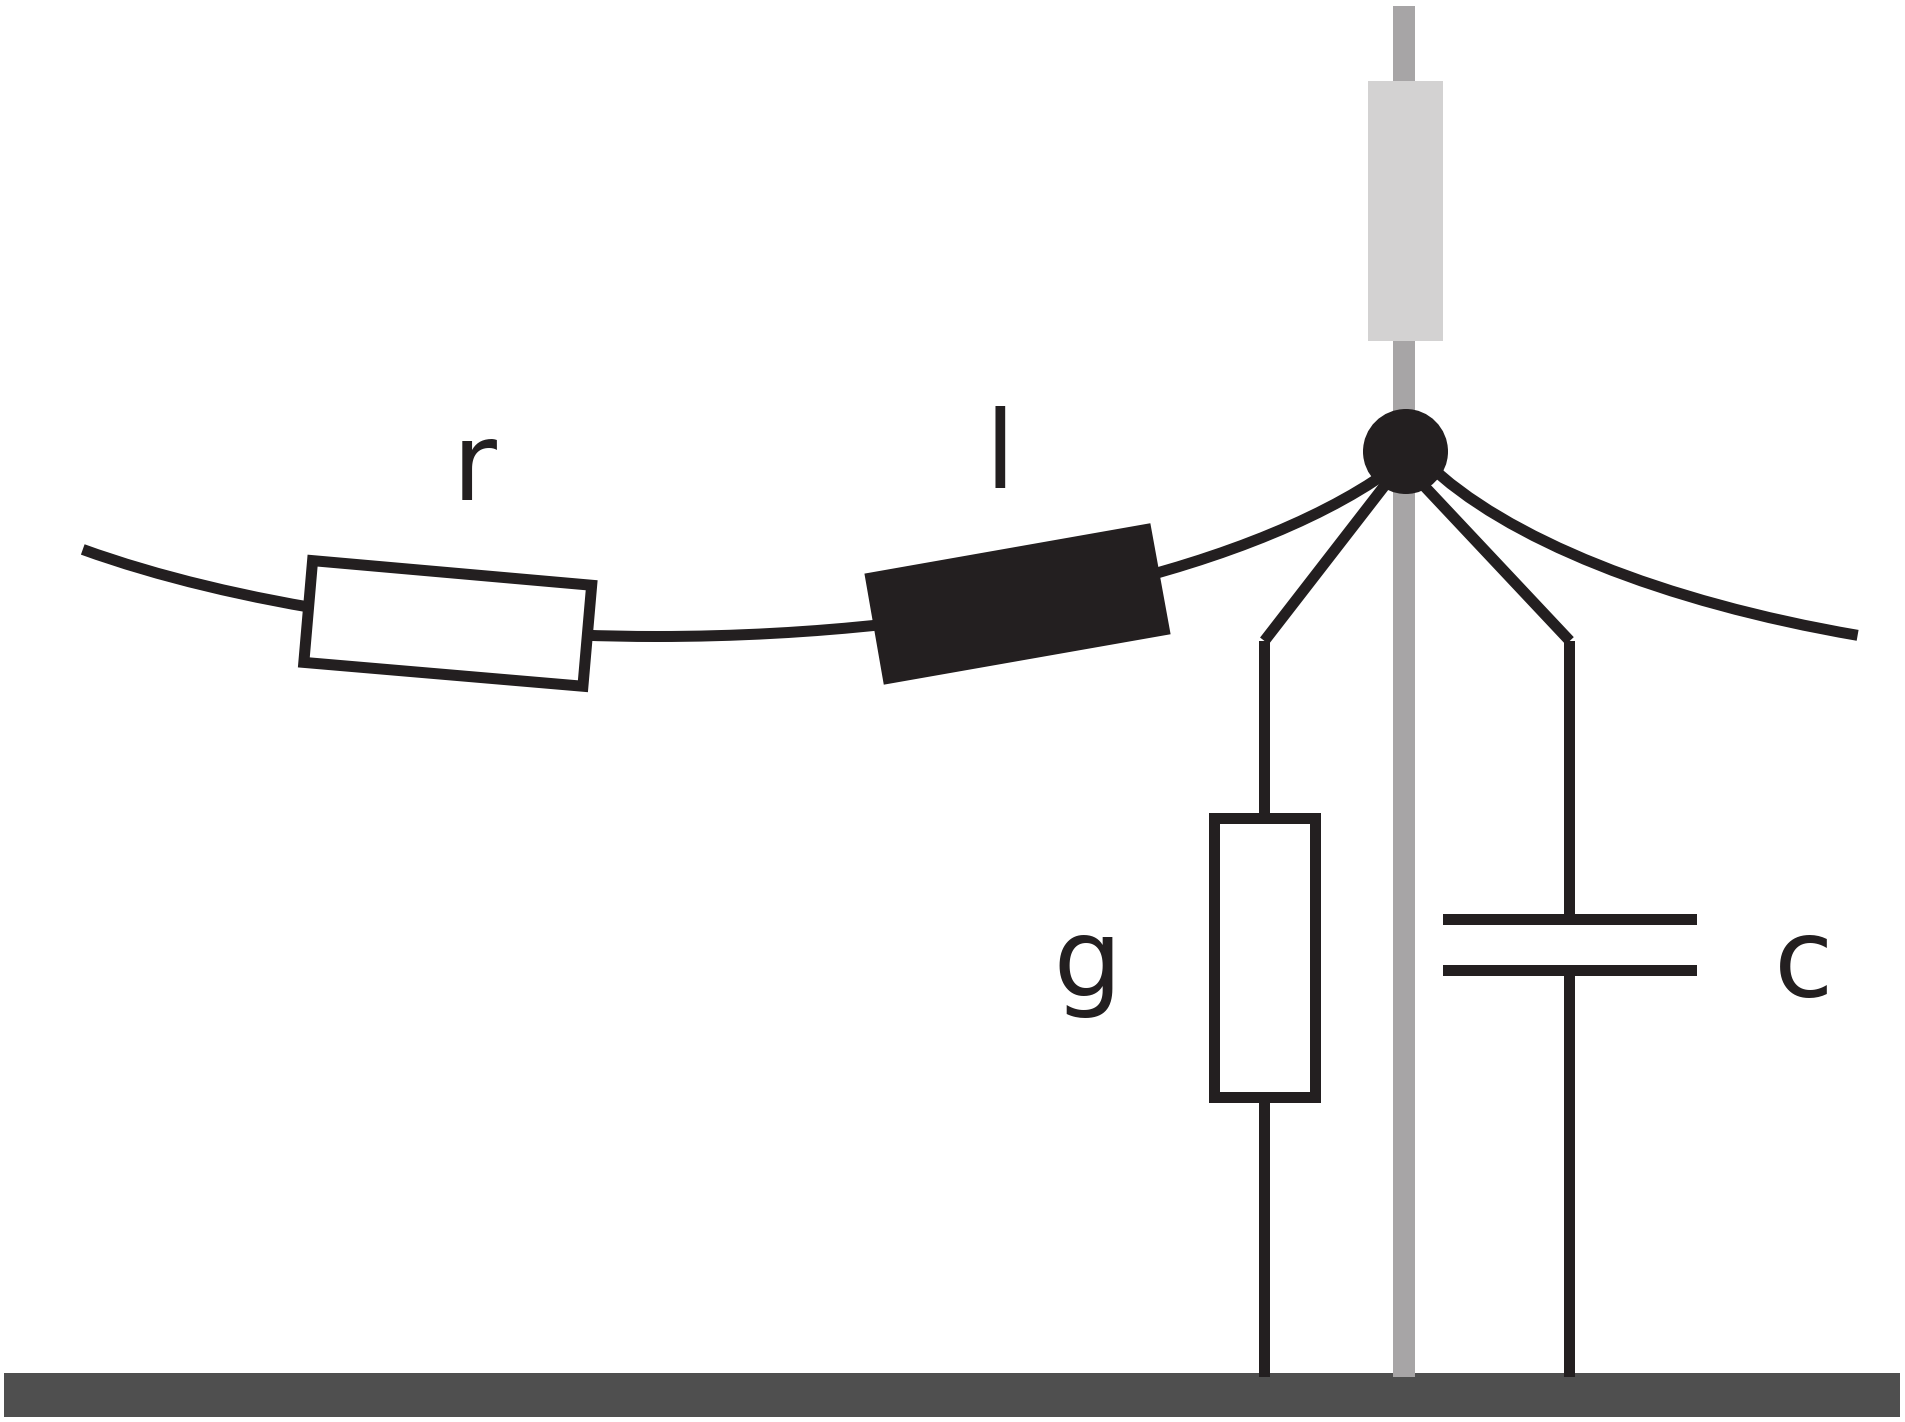
\includegraphics[width=0.7\columnwidth, align=c]{images/Ersatzschaltbild.png}
    \begin{minipage}[c]{0.3\columnwidth}
        \begin{itemize}
            \item Widerstandsbelag (r)
            \item Induktivitätsbelag (l)
            \item Ableitbelag (g)
            \item Kapazitätsbelag (c)
        \end{itemize}
    \end{minipage}


    \subsection{Widerstandsbelag r}
    % \newcolumn
    \subsubsection{Ursache}
    \begin{itemize}
        \item Ohmscher Widerstand des Leiterseils
        \item Bei \textbf{Wechselstrom} $\Rightarrow$ Berücksichtigung der \textbf{Stromverdrängung} (\textit{skin-effect})
    \end{itemize}


\subsubsection{Temperaturabhängigkeit des Widerstands}
    Der spezifische Widerstand $\rho$ ist temperaturabhängig und ergibt sich aus:

    \vspace{0.15cm}

    \begin{minipage}[t]{0.33\columnwidth}
        $
        \boxed{
        \rho = \rho_{\qty{20}{\degree}} \cdot \left[ 1 + \alpha \cdot \left(T - \qty{20}{\degree}\right) \right]
        }
        $ 
    \end{minipage}%
    \hfill
    \begin{minipage}[t]{0.65\columnwidth}
        \renewcommand{\arraystretch}{1.2}
        \begin{tabular}{l l l}
            $[\rho]$                    & Spezifischer Widerstand \dotfill                                & $\unit[per-mode=fraction]{\ohm\milli\metre\squared\per\metre}$ \\
            $[\rho_{\qty{20}{\degree}}]$& Spezifischer Widerstand bei $\qty{20}{\degreeCelsius}$ \dotfill & $\unit[per-mode=fraction]{\ohm\milli\metre\squared\per\metre}$ \\
            $[\alpha]$                  & Temperaturkoeffizient \dotfill                                  & $\unit[per-mode=fraction]{\per\degreeCelsius}$ \\
            $[T]$                       & Temperatur \dotfill                                             & $\unit{\degreeCelsius}$ \\
        \end{tabular}
    \end{minipage}

\subsubsection{Ohmscher Widerstand des Leiterseils}
    Der spezifische Widerstand $R'$ eines Leiterseils in $\frac{\Omega}{\text{m}}$ ergibt sich zu:

    \vspace{0.15cm}

    \begin{minipage}[t]{0.33\columnwidth}
        $
        \boxed{
        R' = \sigma \cdot \frac{\rho}{A}
        }
        $
    \end{minipage}%
    \hfill
    \begin{minipage}[t]{0.65\columnwidth}
        \renewcommand{\arraystretch}{1.2}
        \begin{tabular}{l l l}
            $[R']$      & Ohmscher Widerstand pro Meter \dotfill                & $\unit[per-mode=fraction]{\ohm\per\metre}$ \\
            $[\sigma]$  & Verseilfaktor (typisch $\sigma = 1{,}07$) \dotfill    & $-$ \\
            $[\rho]$    & Leitfähigkeit (spezifischer Widerstand) \dotfill      & $\unit[per-mode=fraction]{\ohm\milli\metre\squared\per\metre}$ \\
            $[A]$       & Leiterquerschnitt \dotfill                            & $\unit{\milli\metre\squared}$ \\
        \end{tabular}
    \end{minipage}

\subsection{Skin-Effekt}
    Die Eindringtiefe $\delta$ des elektrischen Feldes in einen Leiter ergibt sich zu:

    \vspace{0.15cm}

    \begin{minipage}[t]{0.33\columnwidth}
        $
        \boxed{
        \delta  = \sqrt{\frac{2 \cdot \rho}{\omega \cdot \mu}}
                = \sqrt{\frac{\rho}{\pi \cdot f \cdot \mu}}
        }
        $
    \end{minipage}%
    \hfill
    \begin{minipage}[t]{0.65\columnwidth}
        \renewcommand{\arraystretch}{1.2}
        \begin{tabular}{l l l}
            $[\delta]$   & Eindringtiefe des Stroms (Skin-Tiefe) \dotfill   & $\unit{\metre}$ \\
            $[\rho]$     & Spez. Widerstand des Leitermaterials \dotfill    & $\unit{\ohm\metre}$ \\
            $[\omega]$   & Kreisfrequenz \dotfill                           & $\unit[per-mode=fraction]{\radian\per\second}$ \\
            $[\mu]$      & Permeabilität des Leitermaterials \dotfill       & $\unit[per-mode=fraction]{\henry\per\metre}$ \\
        \end{tabular}
    \end{minipage}

    \vspace{0.1cm}

    \textit{\textbf{Bündelleiter} schwächen den Skin-Effekt durch die Aufspaltung des Querschnitts ab.}



\subsection{Ableitungsbelag g}
    \begin{itemize}
        \item Ensteht durch Verluste des Dielektrikums zwischen L-L und zwischen L-PE
        \item $G'$ ist sehr klein $\rightarrow$ bei norm. Betriebsverhältnissen gegenüber $\omega C'$ \textbf{vernachlässigbar}
        \item $G'$ ist grösser wenn Teilentladungen (Corona-Effekt) auftreten
        \item \textbf{Witterungsabhängig}
    \end{itemize}

\subsection{Induktivitätsbelag l}
    \begin{minipage}[t]{0.49\columnwidth}
        \begin{itemize}
            \item Entsteht durch Verkettung der magnetischen Flüsse
            \item Strom in L1 hat magnetische Flussverkettung zur Folge
            \item Fluss = verursachender Strom $\times$ Induktivität
        \end{itemize}
    \end{minipage}%
    \hfill
    \begin{minipage}[t]{0.49\columnwidth}
        \centering \vspace{-0.7\baselineskip}
        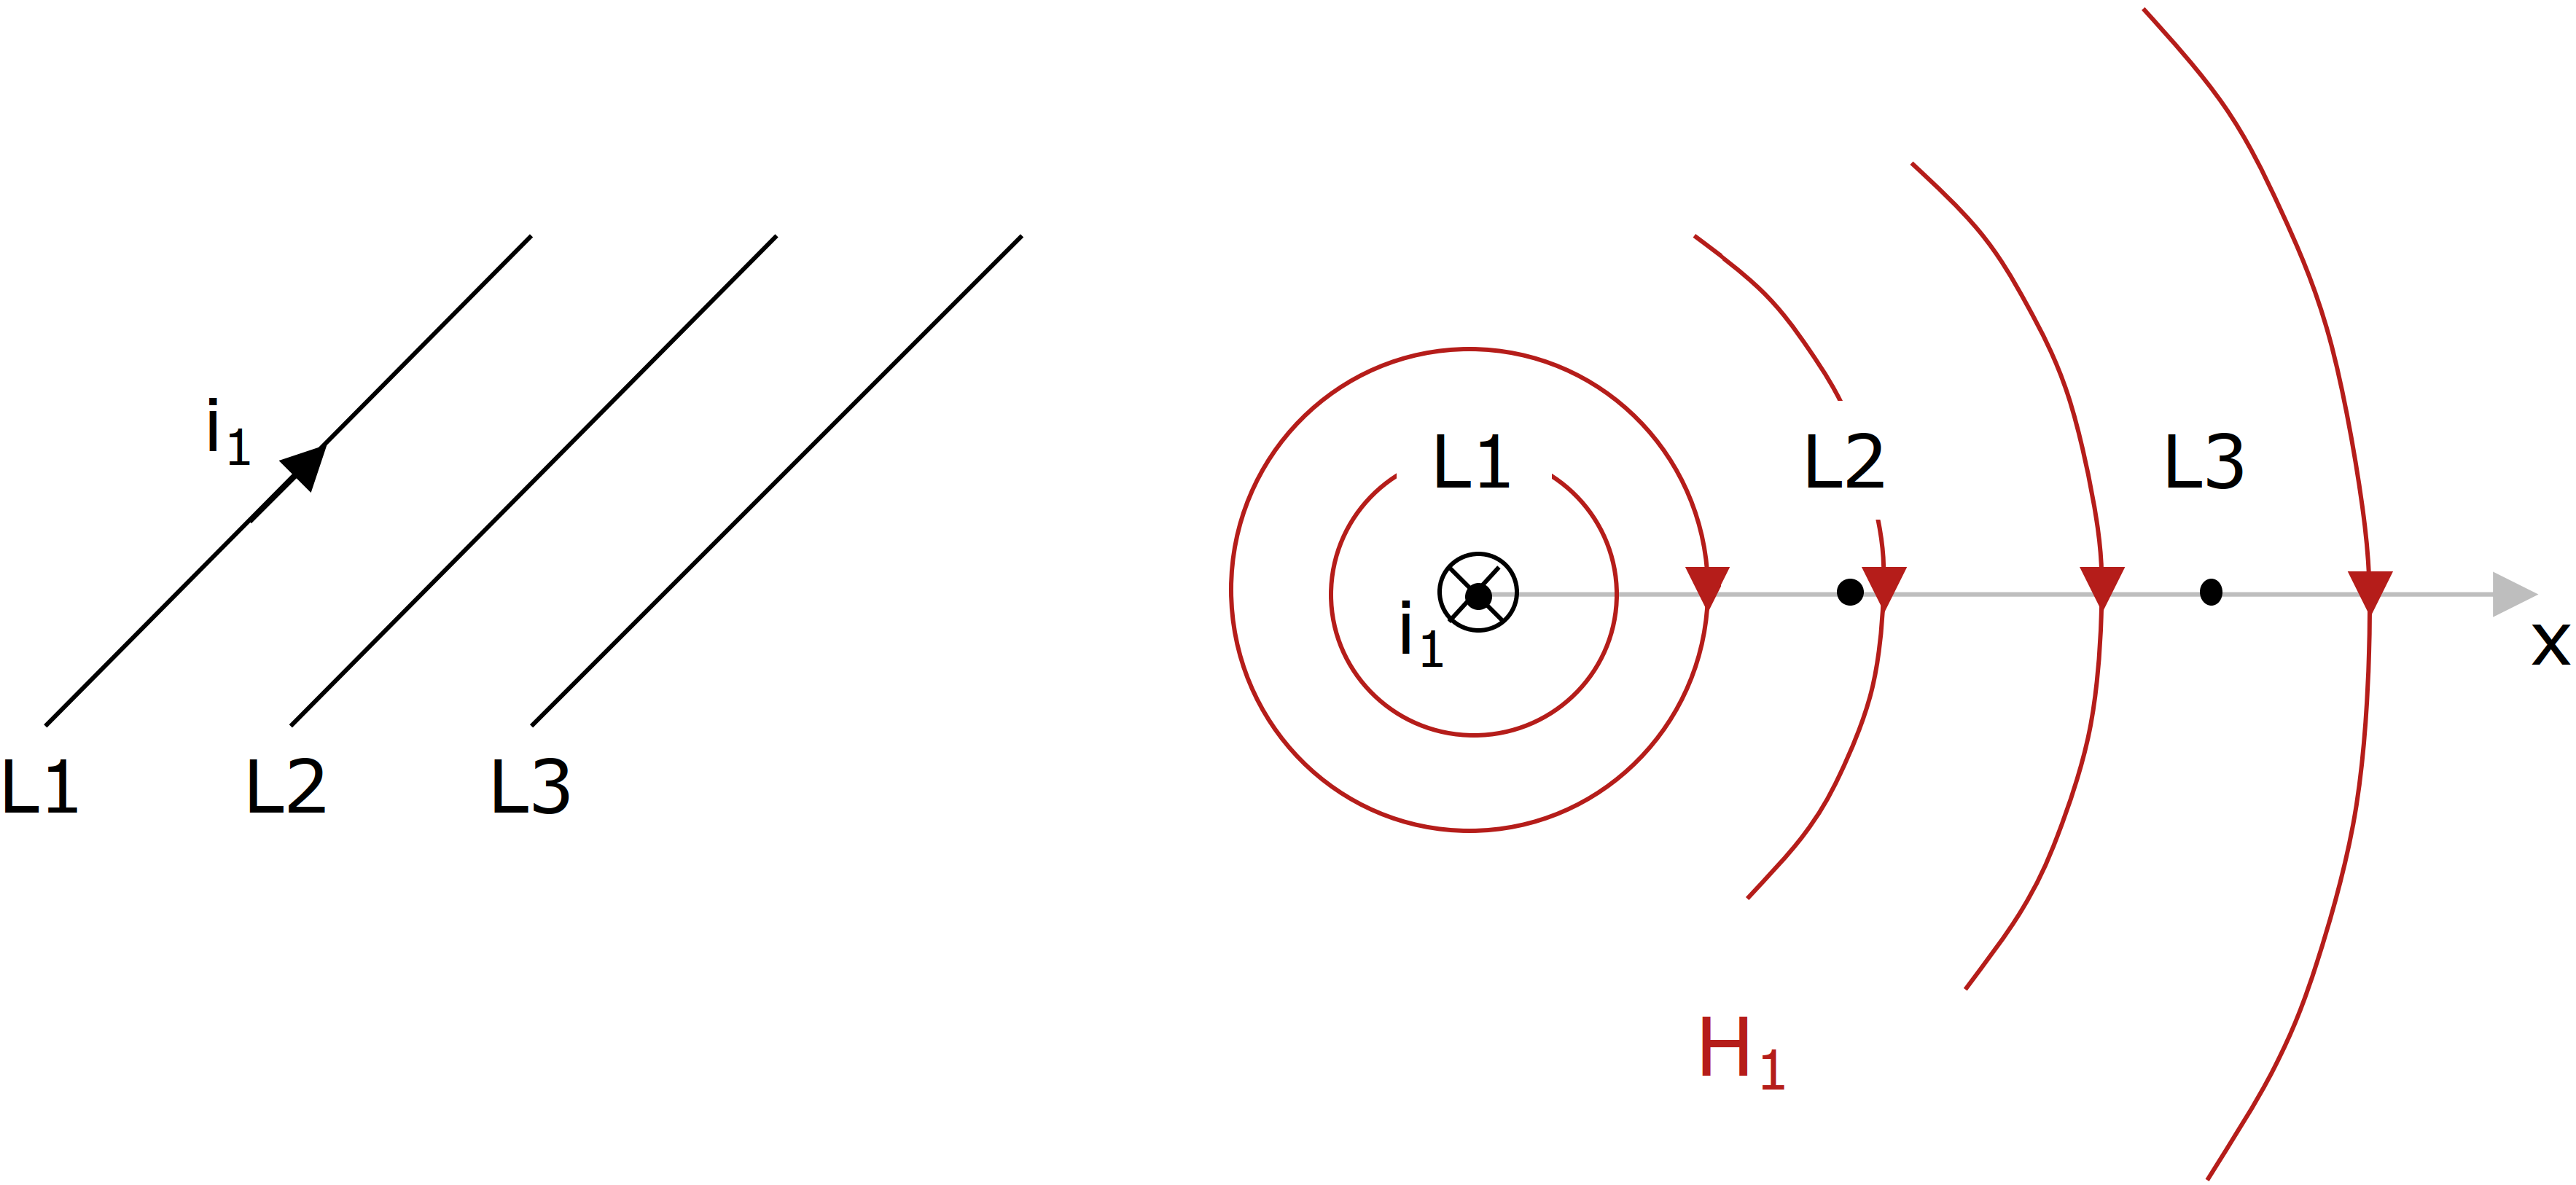
\includegraphics[width=0.9\columnwidth, align=c]{images/Induktivitätsbelag_1.png}
    \end{minipage}



\subsubsection{Herleitung}
    \begin{minipage}[t]{0.44\columnwidth}
        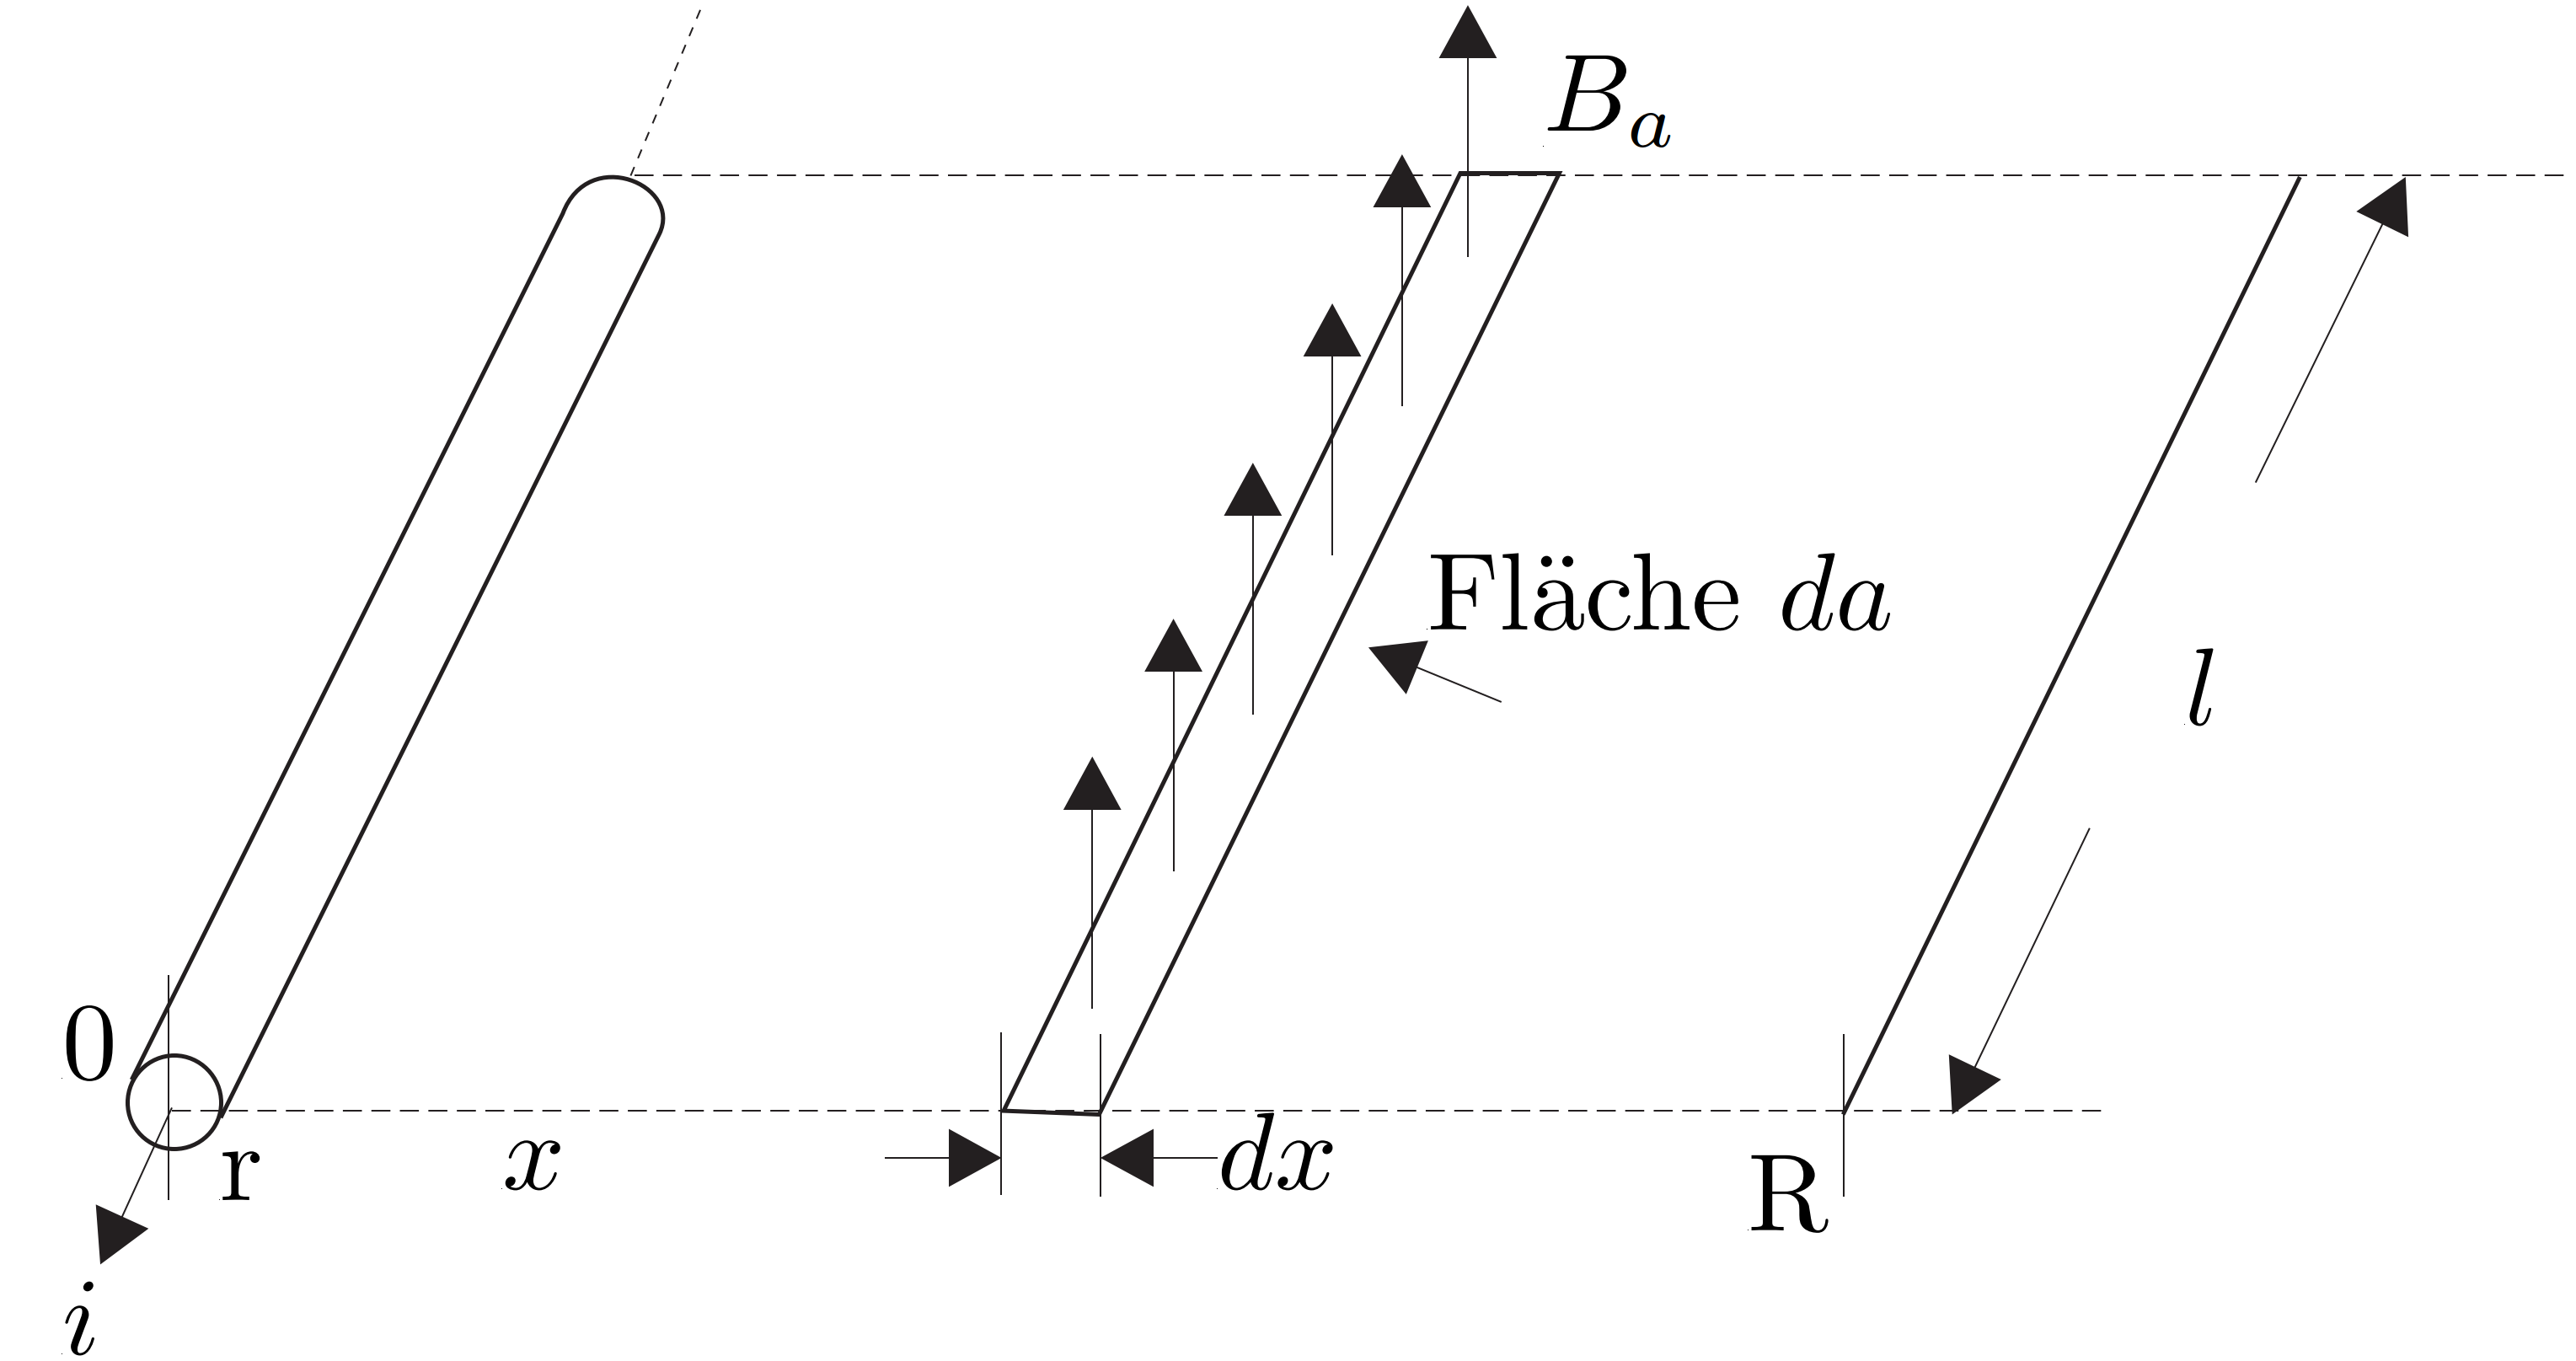
\includegraphics[width=0.9\columnwidth, align=c]{images/Induktivitätsbelag_2.png}
    \end{minipage}%
    \hfill
    \begin{minipage}[t]{0.55\columnwidth}
        $
        \begin{tabular}{rcl}
            $\phi_1$    &=& $\displaystyle \int_A B_1(x)\, da = \int_r^R B_1(x)\, dx$ \\
            $da$        &=& $l\, dx$ \\
            $B_1(x)$    &=& $\mu_0 H_1(x) \quad \text{and} \quad H_1(x) = \dfrac{i}{2\pi x}$ \\
            $\phi_1$    &=& $\mu_0 \displaystyle \int_r^R \frac{i}{2\pi x} \, l\, dx$ \\
                        &=& $\dfrac{\mu_0 i}{2\pi} \ln \dfrac{R}{r}$ \\
            $\phi_1$    &=& $L_1 i$ \\
            $L_1$       &=& $\dfrac{\mu_0}{2\pi} \ln \dfrac{R}{r}$
        \end{tabular}
        $
    \end{minipage}
\newcolumn

\subsubsection{Formel}
    Der Induktivitätsbelag $L'$ in $\unit[per-mode=symbol]{\henry\per\metre}$ enthält Eigeninduktivität und Kopplungsinduktivität\\
    Annahme: verdrillte Leitung, kreisförmiger Leiterquerschnitt

    \vspace{0.1cm}

    \begin{minipage}[t]{0.33\columnwidth}
        $
        \boxed{L' = \frac{\mu_0}{2 \cdot \pi} \cdot \ln\left( \frac{d}{0{,}78 \cdot r} \right)}
        $

        $
        \boxed{d = \sqrt[3]{d_{12} \cdot d_{23} \cdot d_{31}}}
        $
    \end{minipage}%
    \hfill
    \begin{minipage}[t]{0.65\columnwidth}
        \renewcommand{\arraystretch}{1.2}
        \begin{tabular}{l l l}
            $[L']$     & Induktivitätsbelag \dotfill                            & $\unit[per-mode=fraction]{\henry\per\metre}$ \\
            $[r]$      & Leiterradius \dotfill                                  & $\unit{\metre}$ \\
            $[d]$      & Mittlerer Leiterabstand \dotfill                       & $\unit{\metre}$ \\
            $[d_{ij}]$ & Abstand zwischen Phase $i$ und $j$ \dotfill            & $\unit{\metre}$ \\
            $[\mu_0]$  & Magnetische Feldkonstante $\num{4\pi e-7}$ \dotfill    & $\unit[per-mode=fraction]{\henry\per\metre}$ \\
        \end{tabular}
    \end{minipage}

    \vspace{0.1cm}

\subsubsection{Einfluss Leiterseilabstand auf Längsinduktivität}
    \begin{itemize}
        \item Grösserer Abstand erhöht die Induktivität, da der mag. Kopplungseffekt abnimmt
        \item Kleinere Abstände verringern die Längsinduktivität wegen stärkerer mag. Verkettung zwischen Phasenleitern
    \end{itemize}

    Der Abstand zwischen den Phasen (Leitern) wird von Zentrum zu Zentrum gemessen.

\subsection{Kapazitätsbelag c}
    Verursacht durch Kap. gegenüber anderen Aussenleitern sowie der Umwelt (Mast/Boden)

    \vspace{0.1cm}

    \begin{minipage}[t]{0.33\columnwidth}
        $ \boxed{C' = \frac{2 \pi k}{\ln\left(\frac{d}{r}\right)}}$
    \end{minipage}%
    \hfill
    \begin{minipage}[t]{0.65\columnwidth}
        \renewcommand{\arraystretch}{1.2}
        \begin{tabular}{l l l}
            $[C']$     & Kapazitätsbelag \dotfill                       & $\unit[per-mode=fraction]{\farad\per\metre}$ \\
            $[k]$      & Geometriefaktor \dotfill                       & $-$ \\
                       & (abh. z.\,B. von Masthöhe, Durchhang) \dotfill & \\
            $[d]$      & Mittlerer Leiterabstand \dotfill               & $\unit{\metre}$ \\
            $[r]$      & Leiterradius \dotfill                          & $\unit{\metre}$ \\
        \end{tabular}
    \end{minipage}

    \vspace{0.1cm}

    %     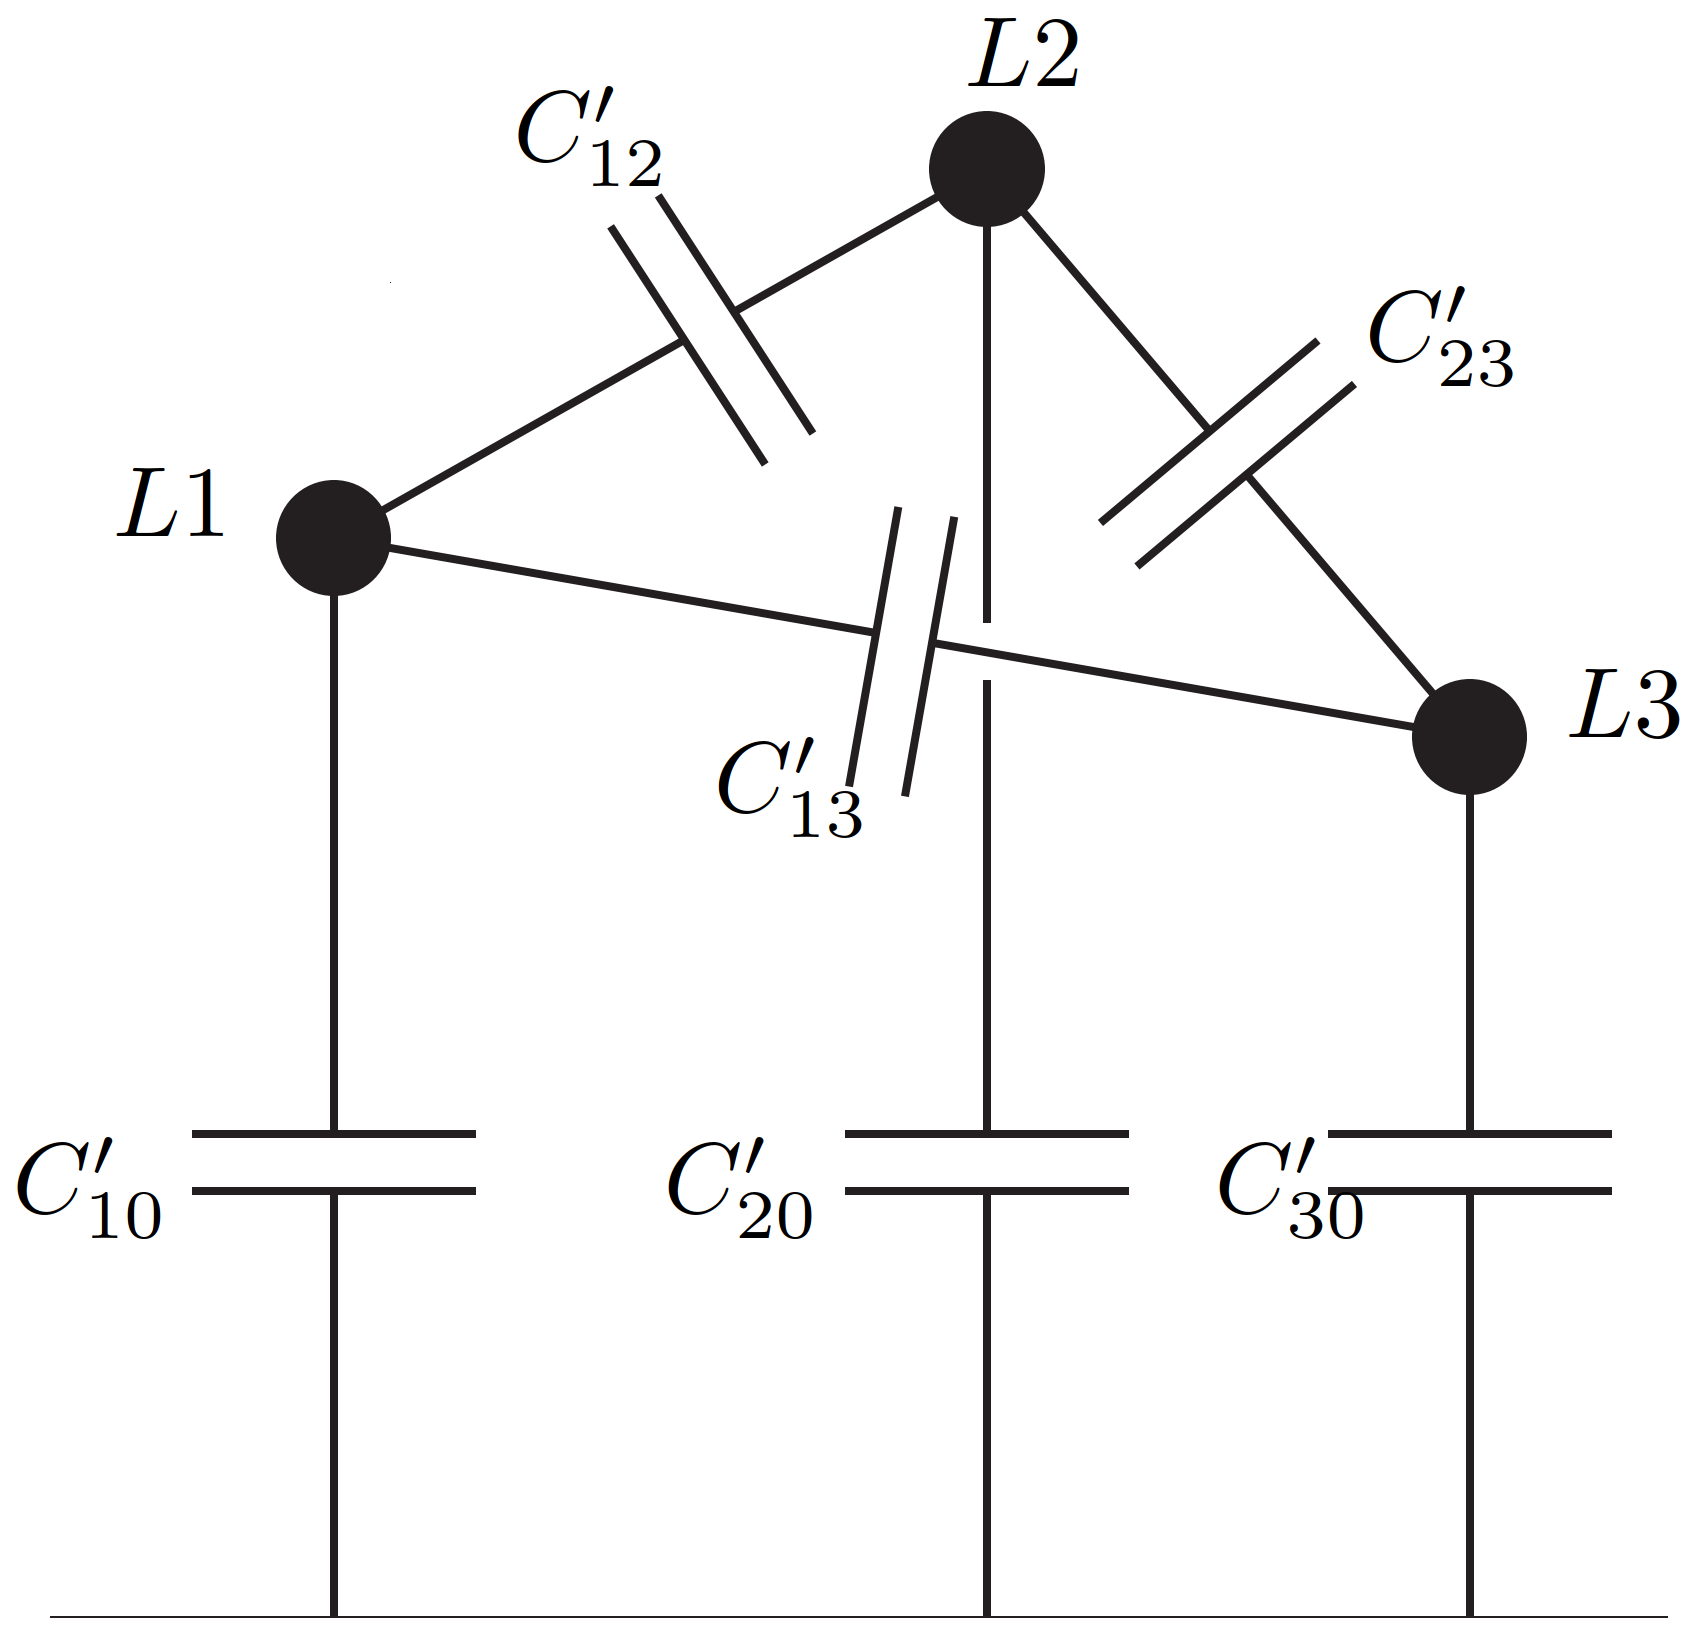
\includegraphics[width=0.35\columnwidth, align=c]{images/Kapazitätsbelag_1.png}

\subsection{Verdrillung}
    \begin{center}
        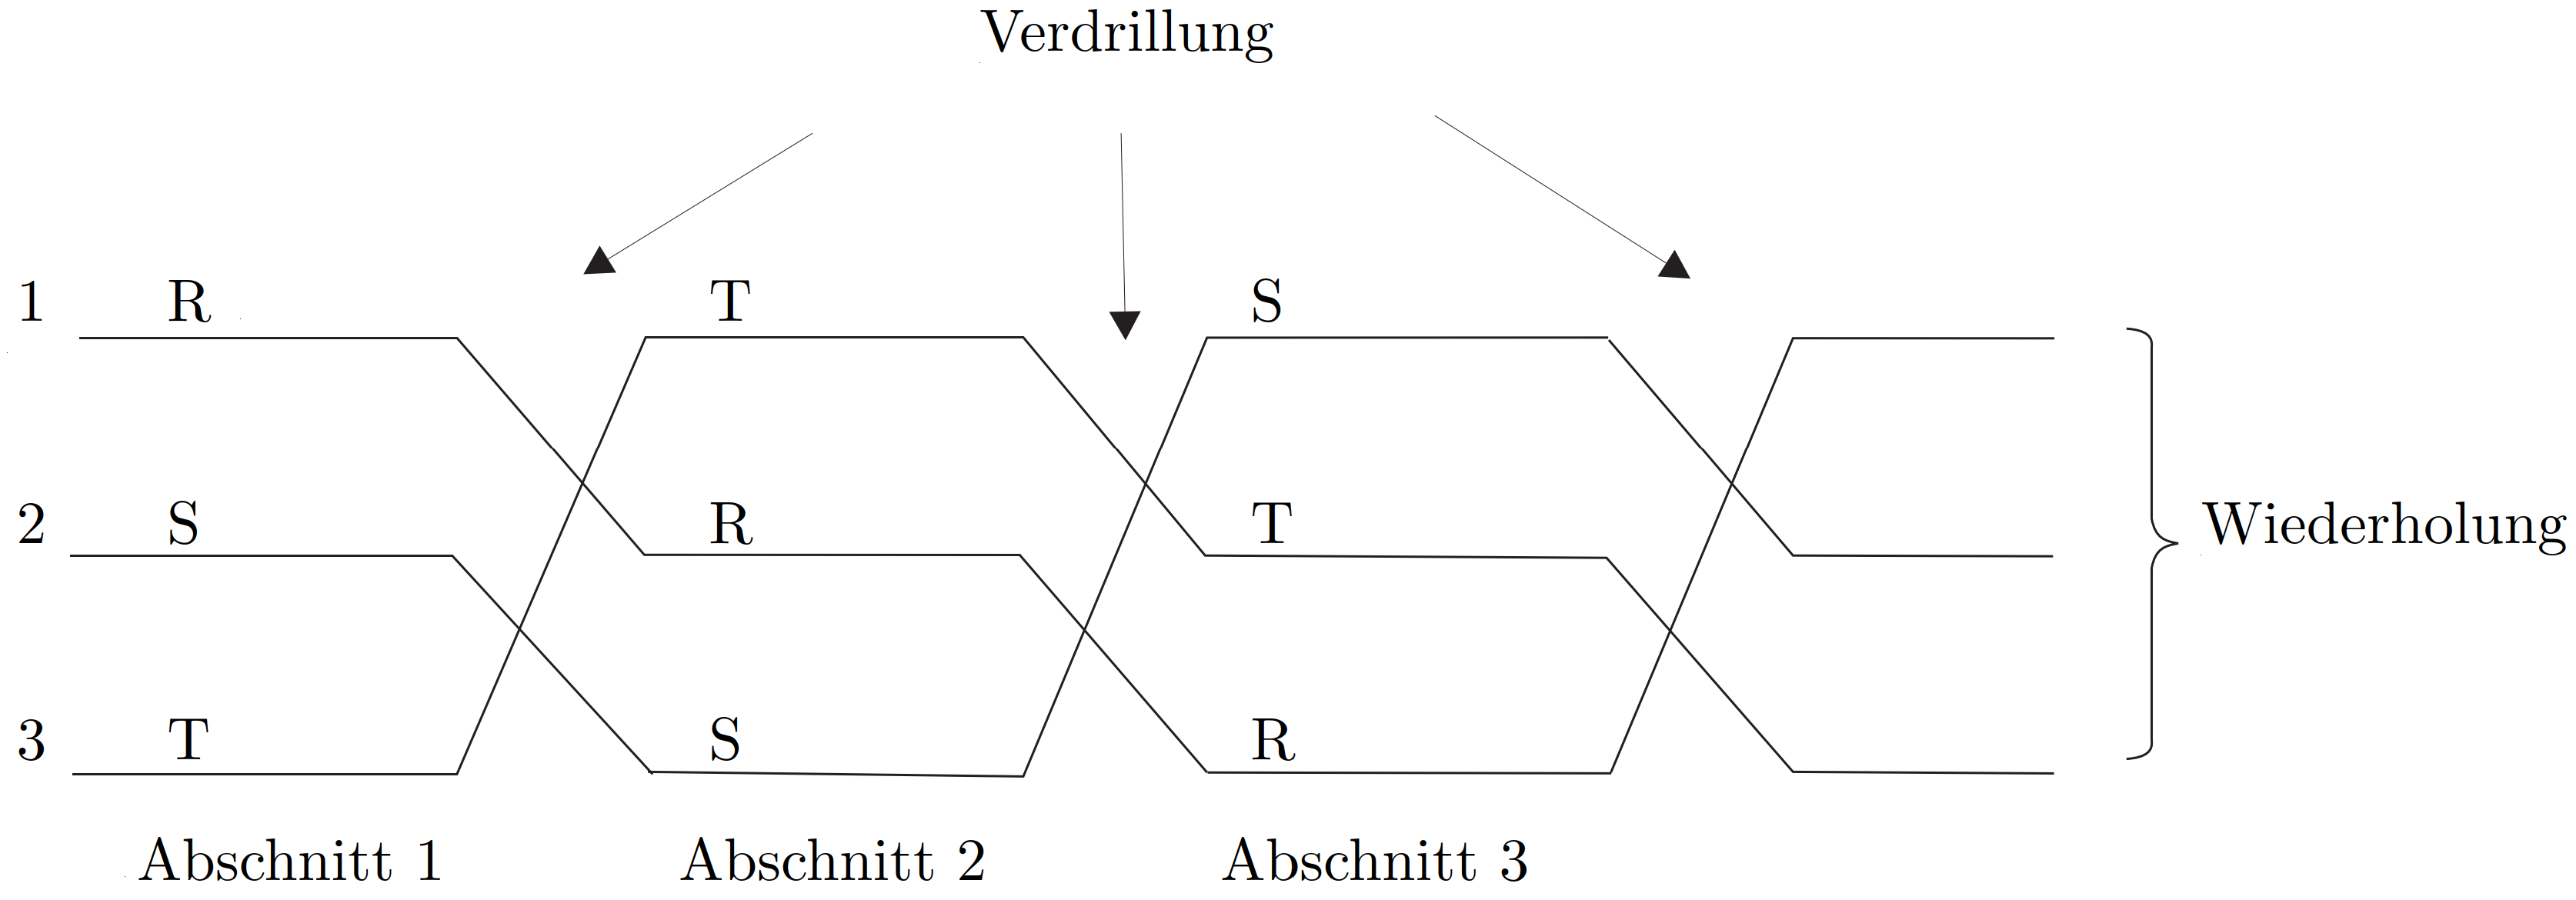
\includegraphics[width=0.9\columnwidth, align=c]{images/Verdrillung.png}
    \end{center}

    % \vspace{0.15cm}

    \begin{itemize}
        \item Die Leiterabstände sind bei einer Freileitung in der Regel nicht alle gleich.
        \item In Bezug auf die Koppelinduktivität ist die Leitung dann nicht symmetrisch.
        \item Man kann sie aber durch Phasentausch nach je einem Drittel der Leitungslänge symmetrisieren (verdrillen).
    \end{itemize}

\subsection{Bündelleiter}
    \begin{center}
        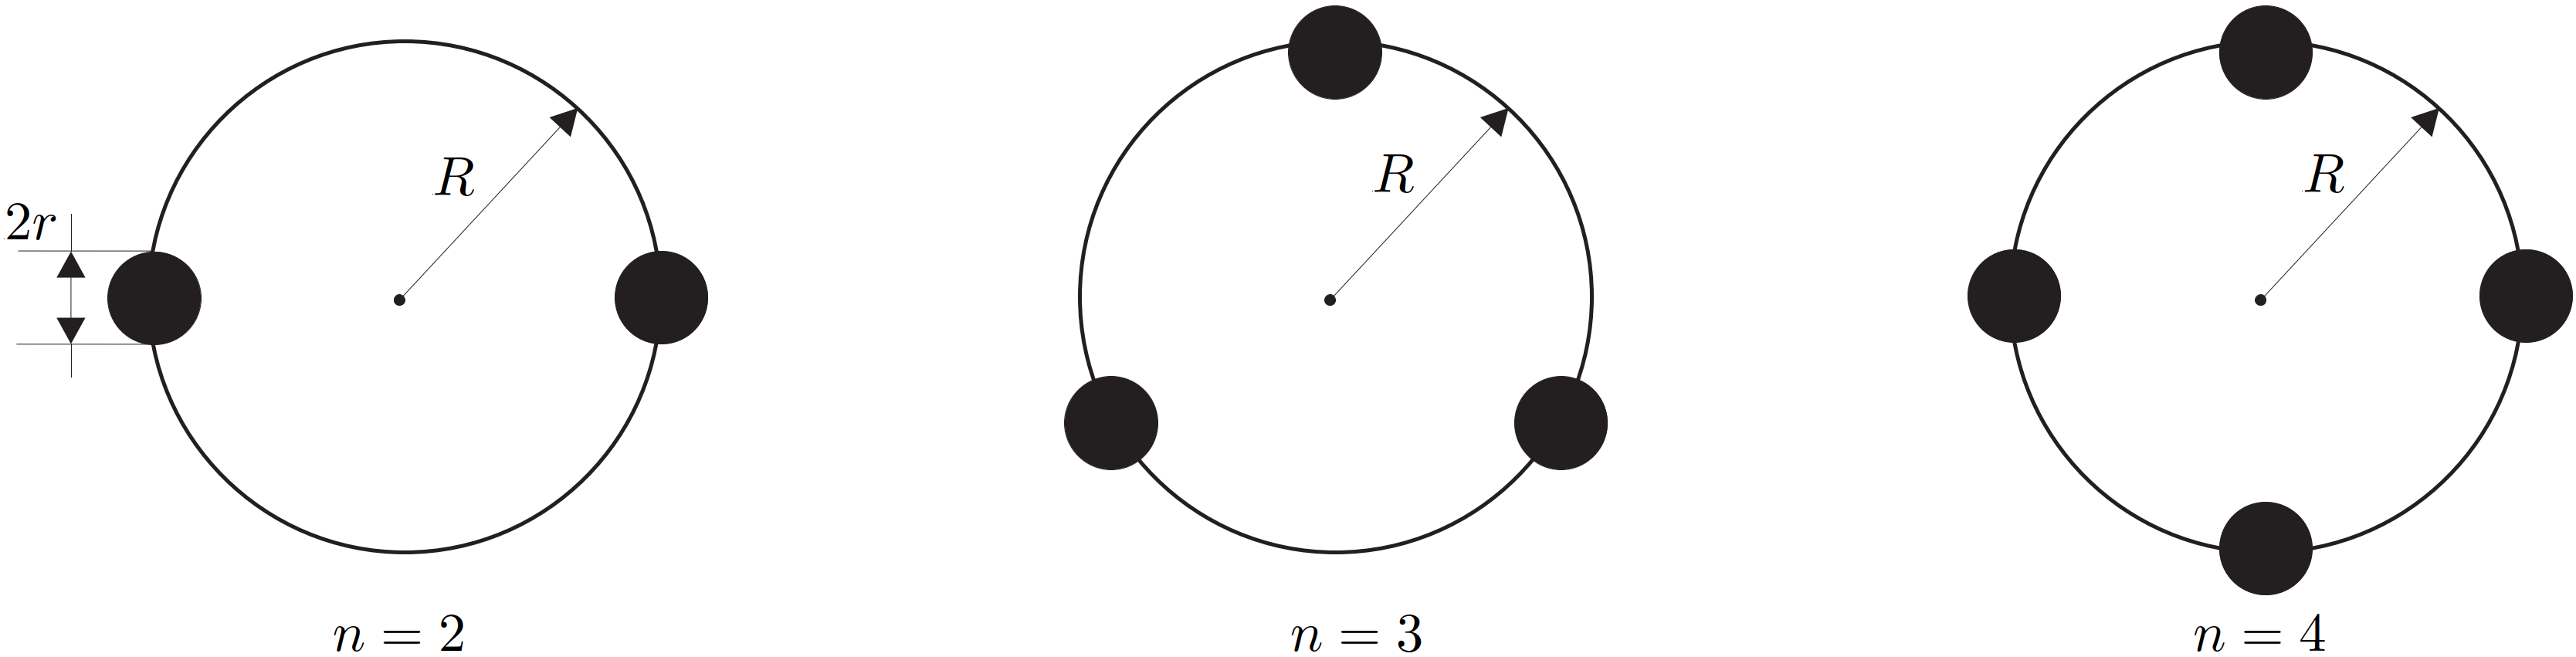
\includegraphics[width=0.98\columnwidth, align=c]{images/Bündelleiter.png}
    \end{center}

    \vspace{0.1cm}

    \begin{minipage}[t]{0.33\columnwidth}
        $ \boxed{r_\text{eq} = \sqrt[n]{n \cdot R^{(n-1)} \cdot r}} $
    \end{minipage}%
    \hfill
    \begin{minipage}[t]{0.65\columnwidth}
        \renewcommand{\arraystretch}{1.2}
        \begin{tabular}{l l l}
            $[r_\text{eq}]$ & Äquivalenter Leiterradius \dotfill                & $\unit{\metre}$ \\
            $[R]$           & Kreisradius der Bündelleiteranordnung \dotfill    & $\unit{\metre}$ \\
            $[r]$           & Teilleiterradius \dotfill                         & $\unit{\metre}$ \\
            $[n]$           & Anzahl der Bündelleiter \dotfill                  & $-$ \\
        \end{tabular}
    \end{minipage}

    \vspace{0.1cm}
 % done
        \section{Leitungsmodell}

\subsection{Leitungsgleichungen}
    \begin{center}
        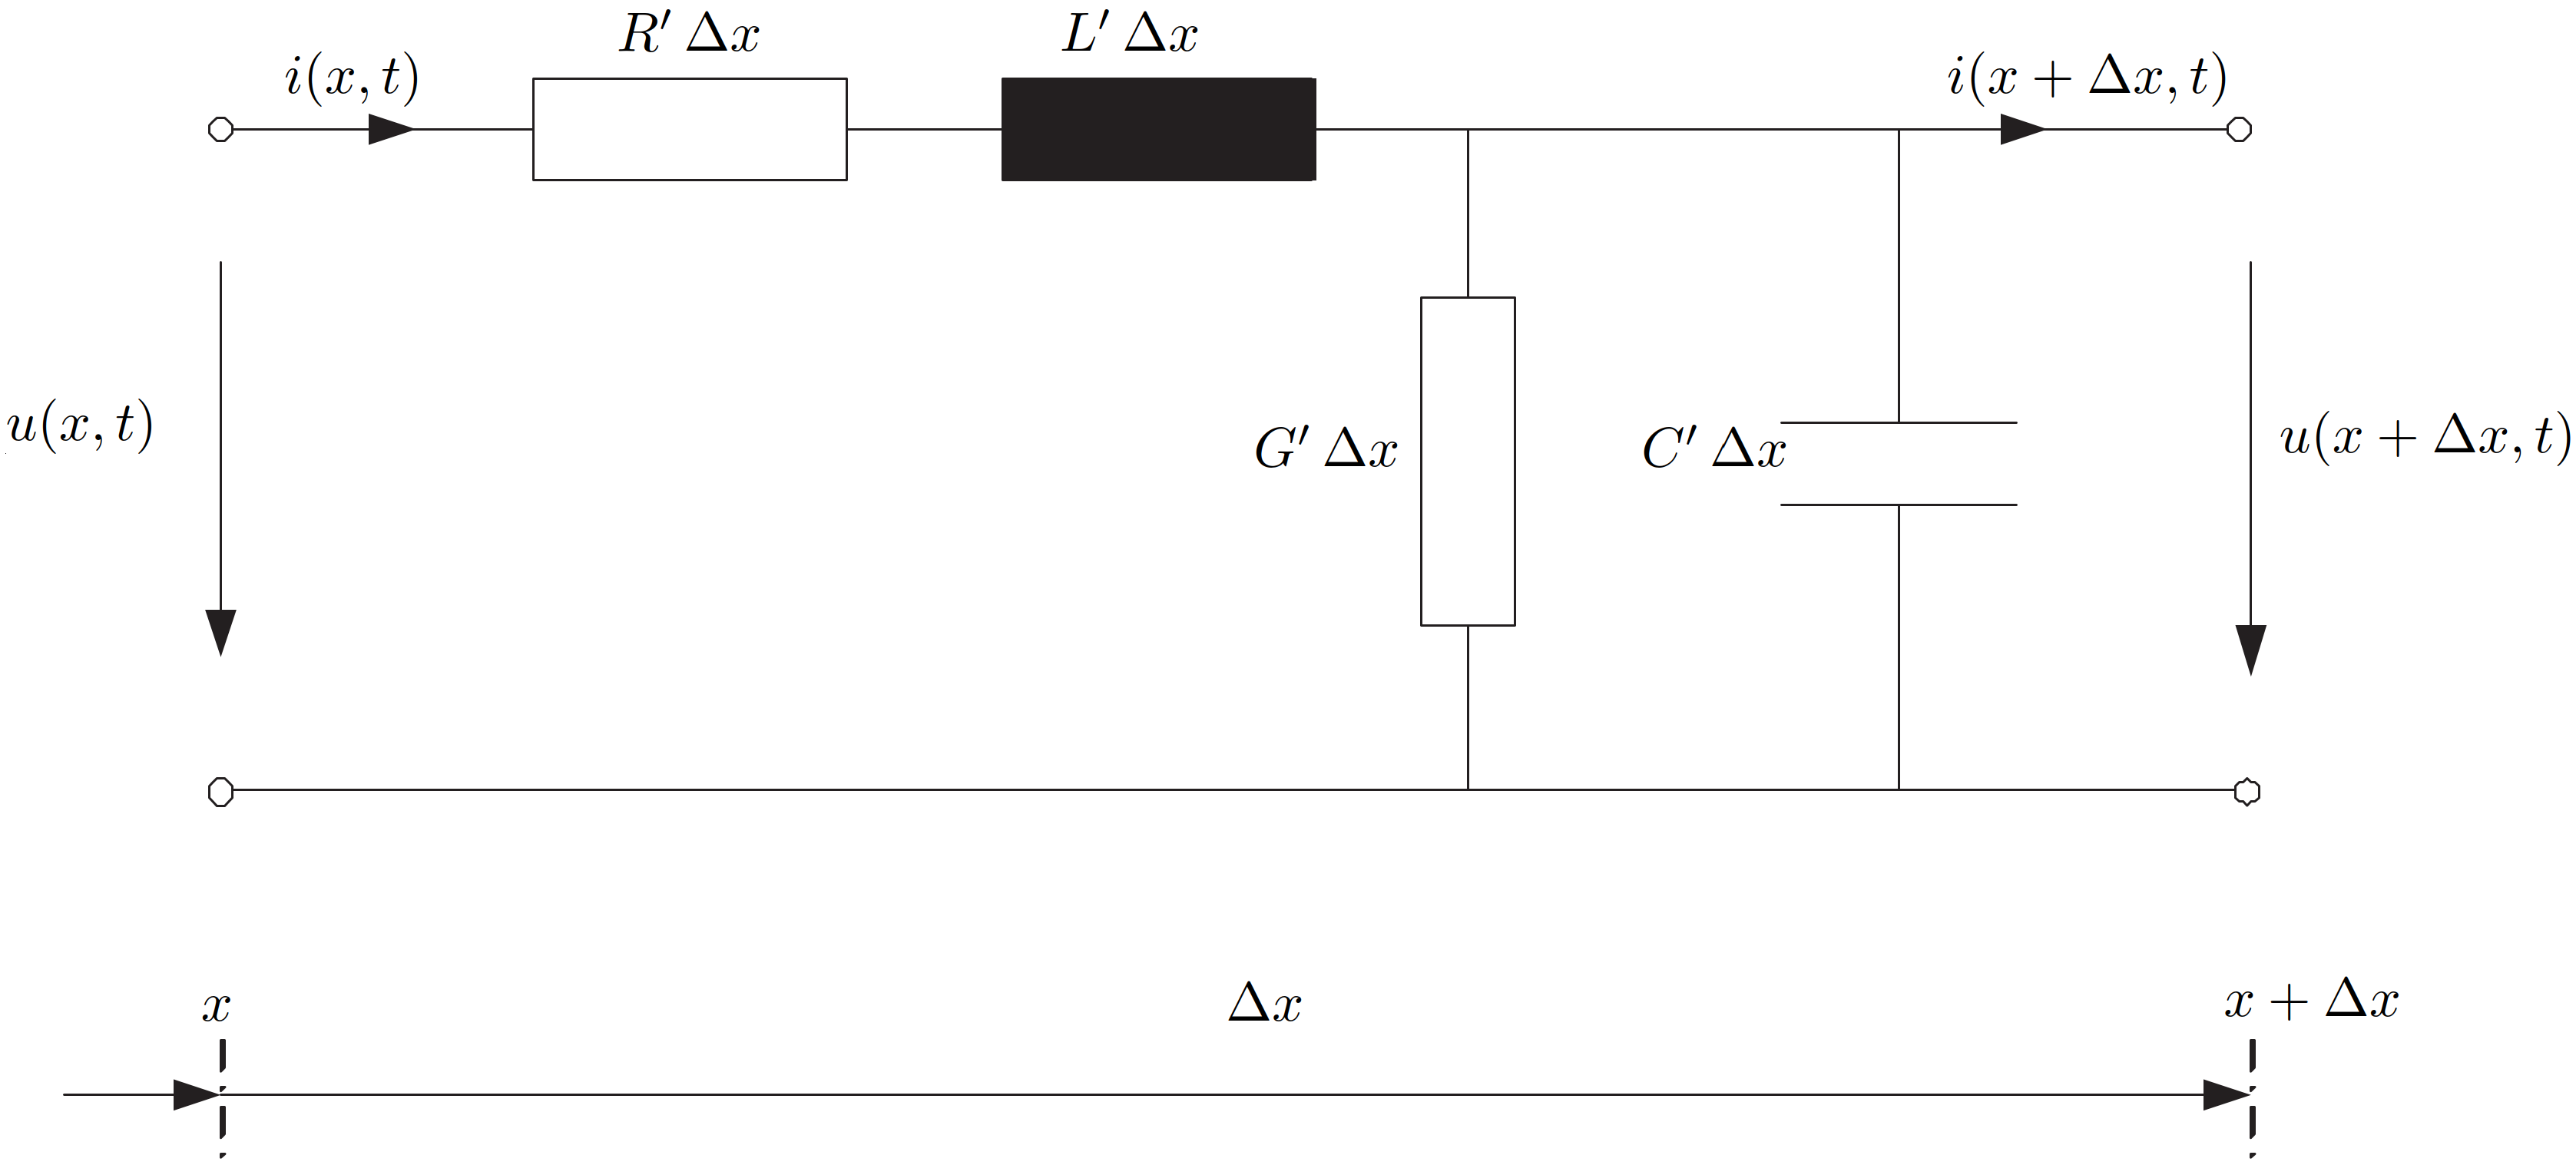
\includegraphics[width=0.95\columnwidth, align=c]{images/Leitungsgleichungen_1.png}
    \end{center}

\subsubsection{Allgemeine Differential Gleichung}
    \vspace{0.1cm}
    $
    \boxed{\frac{\partial u}{\partial x} = -\left(R' + L' \frac{\partial}{\partial t}\right)  \cdot i}
    \quad
    \boxed{\frac{\partial i}{\partial x} = -\left(G' + C' \frac{\partial}{\partial t}\right)  \cdot u}
    $
    \vspace{0.1cm}

\subsubsection{Allgemeine Differential Gleichung für Wechselstrom}
    \vspace{0.1cm}
    $
    \boxed{\frac{\partial U}{\partial x} = -\left(R' \cdot I + j \omega L' \cdot I\right)}
    \quad
    \boxed{\frac{\partial I}{\partial x} = -\left(G' \cdot U + j \omega C' \cdot U\right)}
    $

\subsubsection{Weitere Gleichungen}
    $
    \boxed{\frac{d^2 U}{dx^2} = \left(R' + j \omega L'\right)\left(G' + j \omega C'\right) \cdot U}
    \quad
    \boxed{\frac{d^2 I}{dx^2} = \left(R' + j \omega L'\right)\left(G' + j \omega  C'\right) \cdot I}
    $

    \vspace{0.1cm}

    Mit folgender Definition von $\gamma$ ergibt sich:

    % \vspace{0.1cm}
    $
    \boxed{\underline{\gamma} = \sqrt{(R' + j\omega L')(G' + j \omega C')} = \alpha + j\beta}
    \quad
    \boxed{\frac{d^2 U}{dx^2} = \underline{\gamma}^2 \cdot U}
    \quad
    \boxed{\frac{d^2 I}{dx^2} = \underline{\gamma}^2 \cdot I}
    $

\subsection{Lösung der Leitungsgleichung}
    $
    \boxed{\underline{U}(x) = \underline{U}_a + \underline{U}_b = \underline{U}^+ \cdot e^{-\underline{\gamma} x} + \underline{U}^- \cdot e^{\underline{\gamma} x}}
    \quad
    \boxed{\underline{I}(x) = \underline{I}_a + \underline{I}_b = \underline{I}^+ \cdot e^{-\underline{\gamma} x} + \underline{I}^- \cdot e^{\underline{\gamma} x}}
    $

    $
    \boxed{\underline{I}(x) = \frac{-1}{R' + j\omega L'} \cdot \frac{d\underline{U}}{dx}
    = \sqrt{\frac{G' + j\omega C'}{R' + j\omega L'}} 
    \cdot \left( \underline{U}^+ \cdot e^{-\underline{\gamma} x} - \underline{U}^- \cdot e^{\underline{\gamma} x} \right)}
    $

    $
    \boxed{\underline{Z}_W = \sqrt{\frac{R' + j\omega L'}{G' + j\omega C'}} \quad \ldots \text{ Wellenimpedanz in } \unit{\ohm}}
    $

\subsubsection{Wenn die Spannung der Leitung bekannt ist}
    $
    \boxed{\underline{U}(x = 0) = \underline{U}_1 = \underline{U}^+ + \underline{U}^-}
    \quad
    \boxed{\underline{I}(x = 0) = \underline{I}_1 = \frac{1}{Z_W} \left( \underline{U}^+ - \underline{U}^- \right)}
    $

\subsubsection{Lösen nach $U^+$ und $U^-$}
    $
    \boxed{\underline{U}^+ = \frac{\underline{U}_1 + Z_W \cdot \underline{I}_1}{2}}
    \quad
    \boxed{\underline{U}^- = \frac{\underline{U}_1 - Z_W \cdot \underline{I}_1}{2}}
    $

    $
    \boxed{\underline{U}(x) = \underline{U}_1 \cdot \frac{e^{\underline{\gamma} x} + e^{-\underline{\gamma} x}}{2} 
    - Z_W \cdot \underline{I}_1 \cdot \frac{e^{\underline{\gamma} x} - e^{-\underline{\gamma} x}}{2}}
    $

    $
    \boxed{\underline{U}(x) = \underline{U}_1 \cdot \cosh(\underline{\gamma} x) 
    - Z_W \cdot \underline{I}_1 \cdot \sinh(\underline{\gamma} x)}
    \quad
    \boxed{\underline{I}(x) = \underline{I}_1 \cdot \cosh(\underline{\gamma} x) 
    - \frac{\underline{U}_1}{Z_W} \cdot \sinh(\underline{\gamma} x)}
    $

\subsection{Allgemein und für 50Hz}
\subsubsection{Modell Allgemein mit exakter Zweitor-Gleichung}
    \begin{center}
        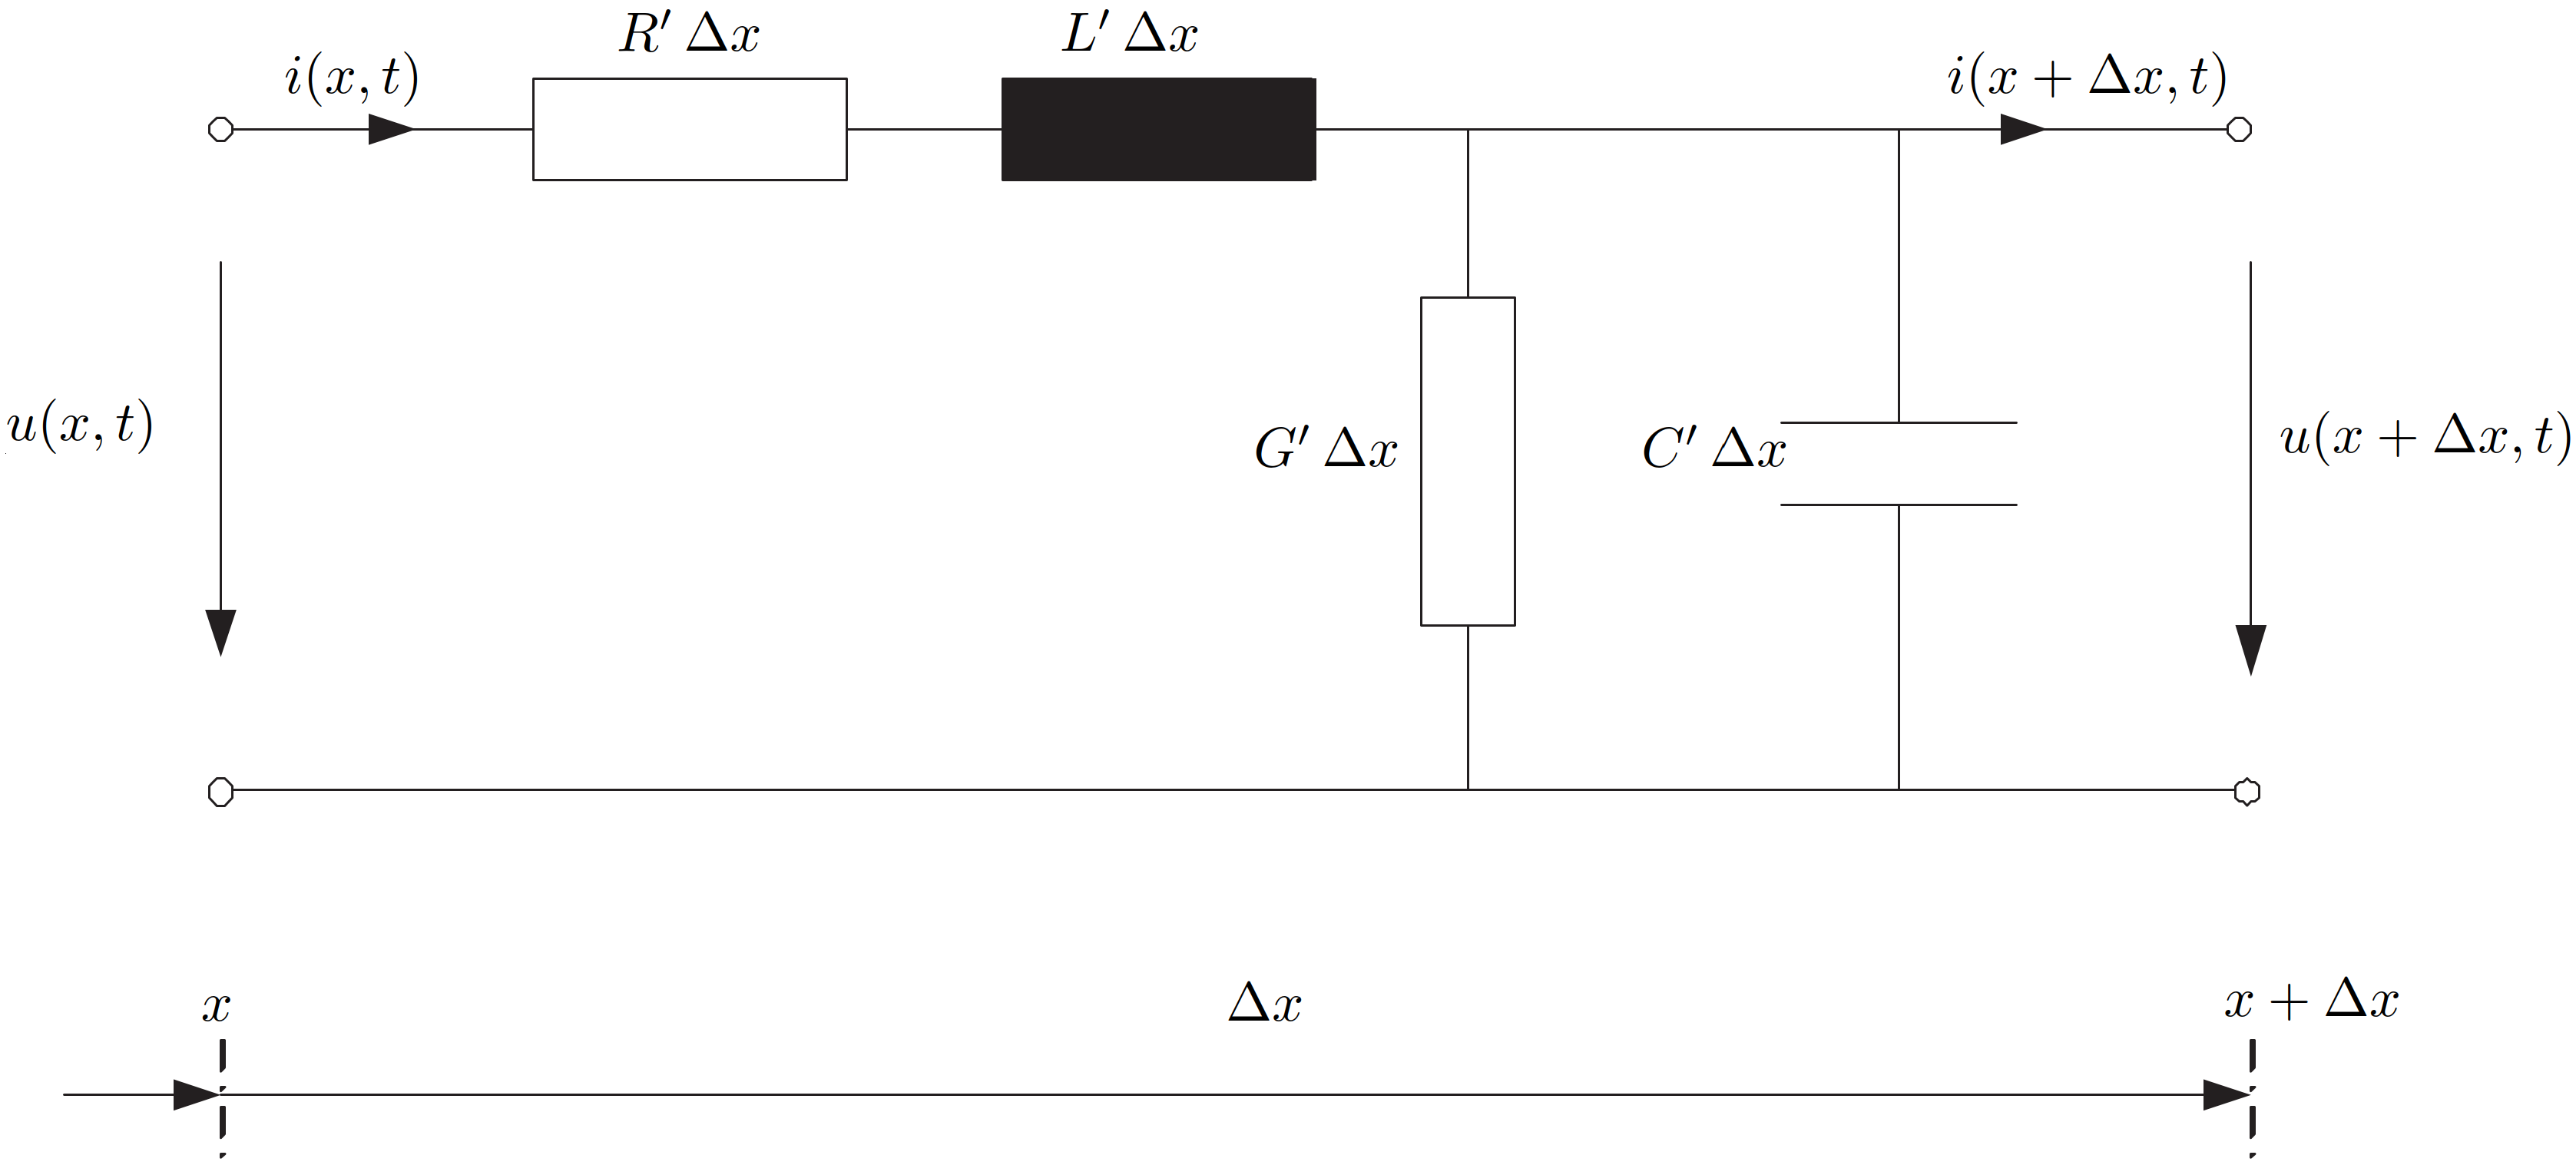
\includegraphics[width=0.95\columnwidth, align=c]{images/Leitungsgleichungen_1.png}
    \end{center}

    \vspace{0.1cm}

    \begin{minipage}[t]{0.58\columnwidth}
        $\boxed{
        \begin{pmatrix}
            \underline{U}_1 \\
            \underline{I}_1
            \end{pmatrix}
            =
            \begin{pmatrix}
            \cosh(\underline{\gamma} \cdot l) & \underline{Z}_W \cdot \sinh(\underline{\gamma} \cdot l) \\
            \frac{1}{\underline{Z}_W} \cdot \sinh(\underline{\gamma} \cdot l) & \cosh(\underline{\gamma} \cdot l)
            \end{pmatrix}
            \begin{pmatrix}
            \underline{U}_2 \\
            \underline{I}_2
        \end{pmatrix}}
        $
    
        $
        \boxed{\underline{\gamma} = \sqrt{(R' + j\omega L')(G' + j \omega C')} = \alpha + j\beta}
        $
    \end{minipage}%
    \hfill
    \begin{minipage}[t]{0.4\columnwidth}
        \textbf{Leerlauf:} $I_2 = 0 \Rightarrow U_2 = \frac{U_1}{\cosh(\gamma l)}$
    
        \textbf{Kurzschl.:} $U_2 = 0 \Rightarrow I_2 = \frac{I_1}{\cosh(\gamma l)}$
    \end{minipage}

\subsection{PI-Ersatzschaltung (Modell Vereinfacht)}
    Wenn $| \underline{\gamma } \cdot l | \ll 1$, kann die Vereinfachung $\cosh{\underline{\gamma l}} \approx 1$ und $\sinh{\underline{\gamma}l} = \underline{\gamma}l$:

    Vereinfachung für „kurze“ Leitungen mit konzentrierten Elementen R, G, L, C
    \begin{itemize}
        \item Querelemente bestehen aus Leitwert und Kapazität
        \item Längselemente bestehen aus Widerstand und Induktivität
        \item 50-Hz-Freileitungen bis ca. 250 km
        \item 50-Hz-Kabel bis ca. 50 km
    \end{itemize}
    \begin{center}
        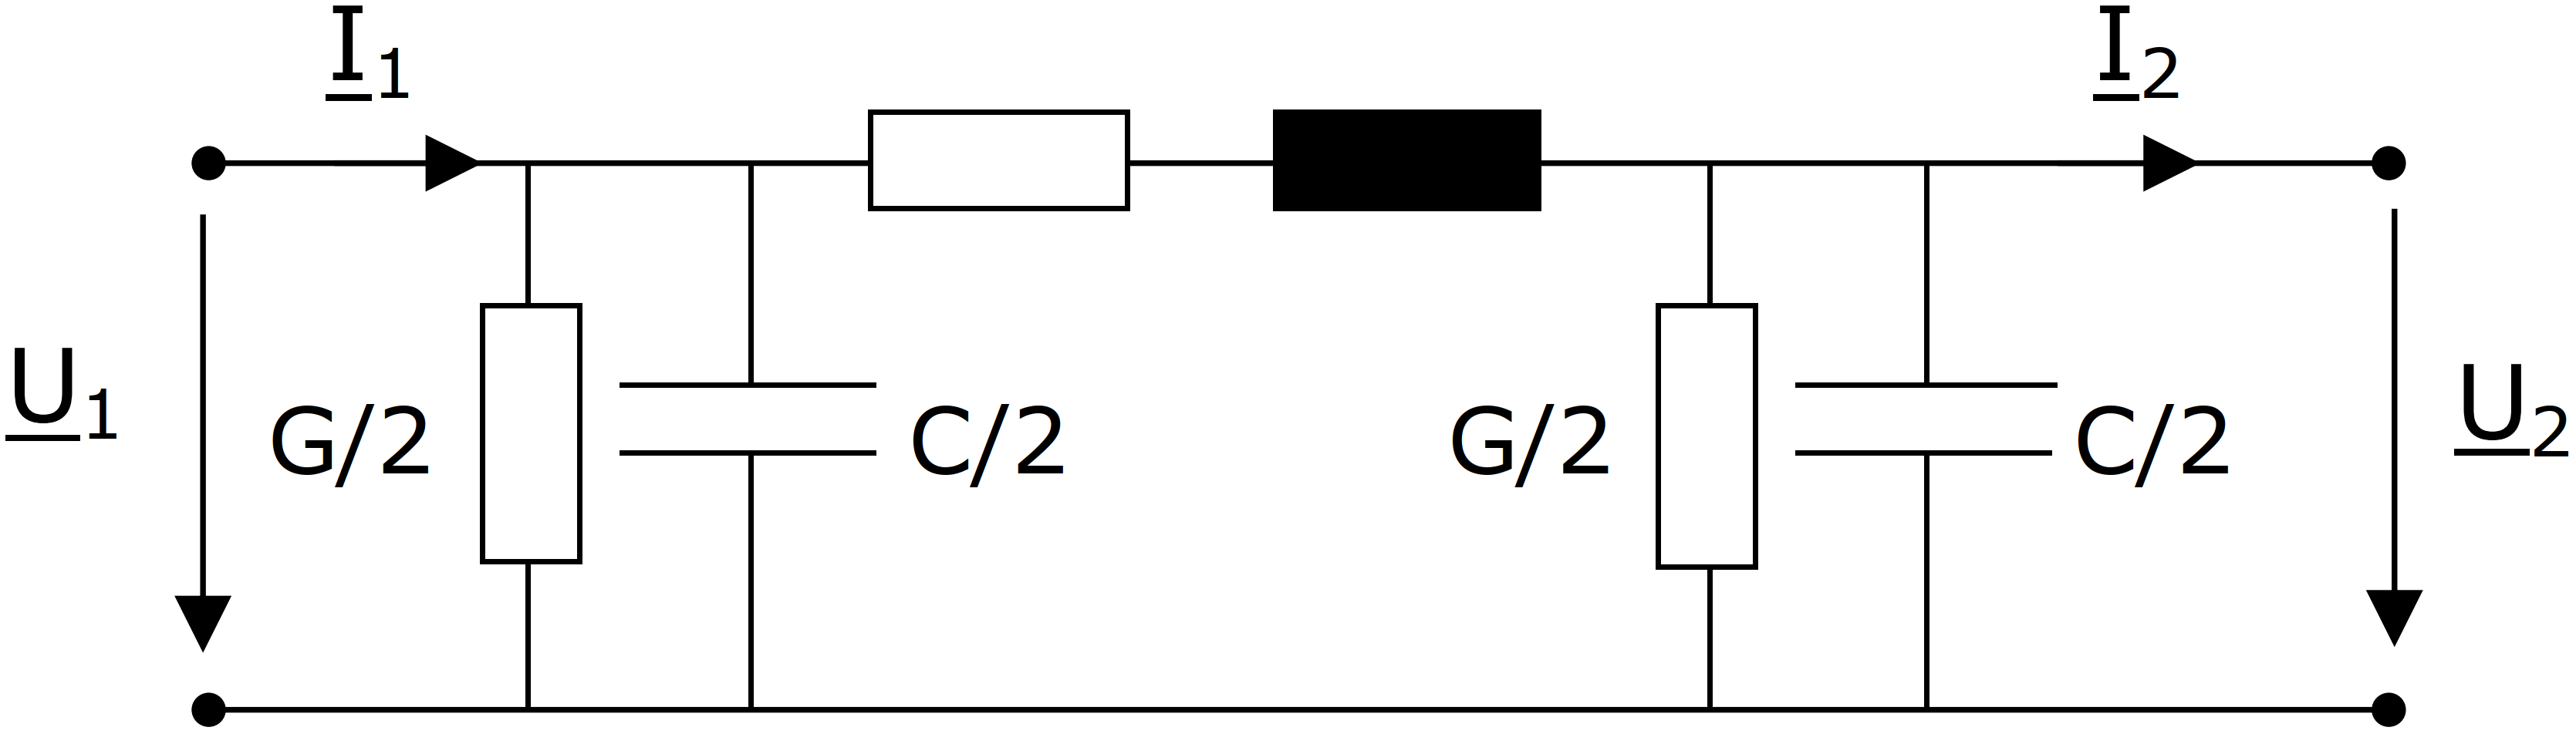
\includegraphics[width=0.9\columnwidth, align=c]{images/Leitungsmodell_gültigkeit.png}
    \end{center}
    \begin{center}
        \centering
                $
                \boxed{
                    \underline{Z} = (R' + j \cdot \omega \cdot L') \cdot l}
                \quad
                \boxed{
                    \dfrac{\underline{Y}}{2} = \dfrac{(G' + j \cdot \omega \cdot C') \cdot l}{2}}
                $ 
    \end{center}

    \begin{center}
        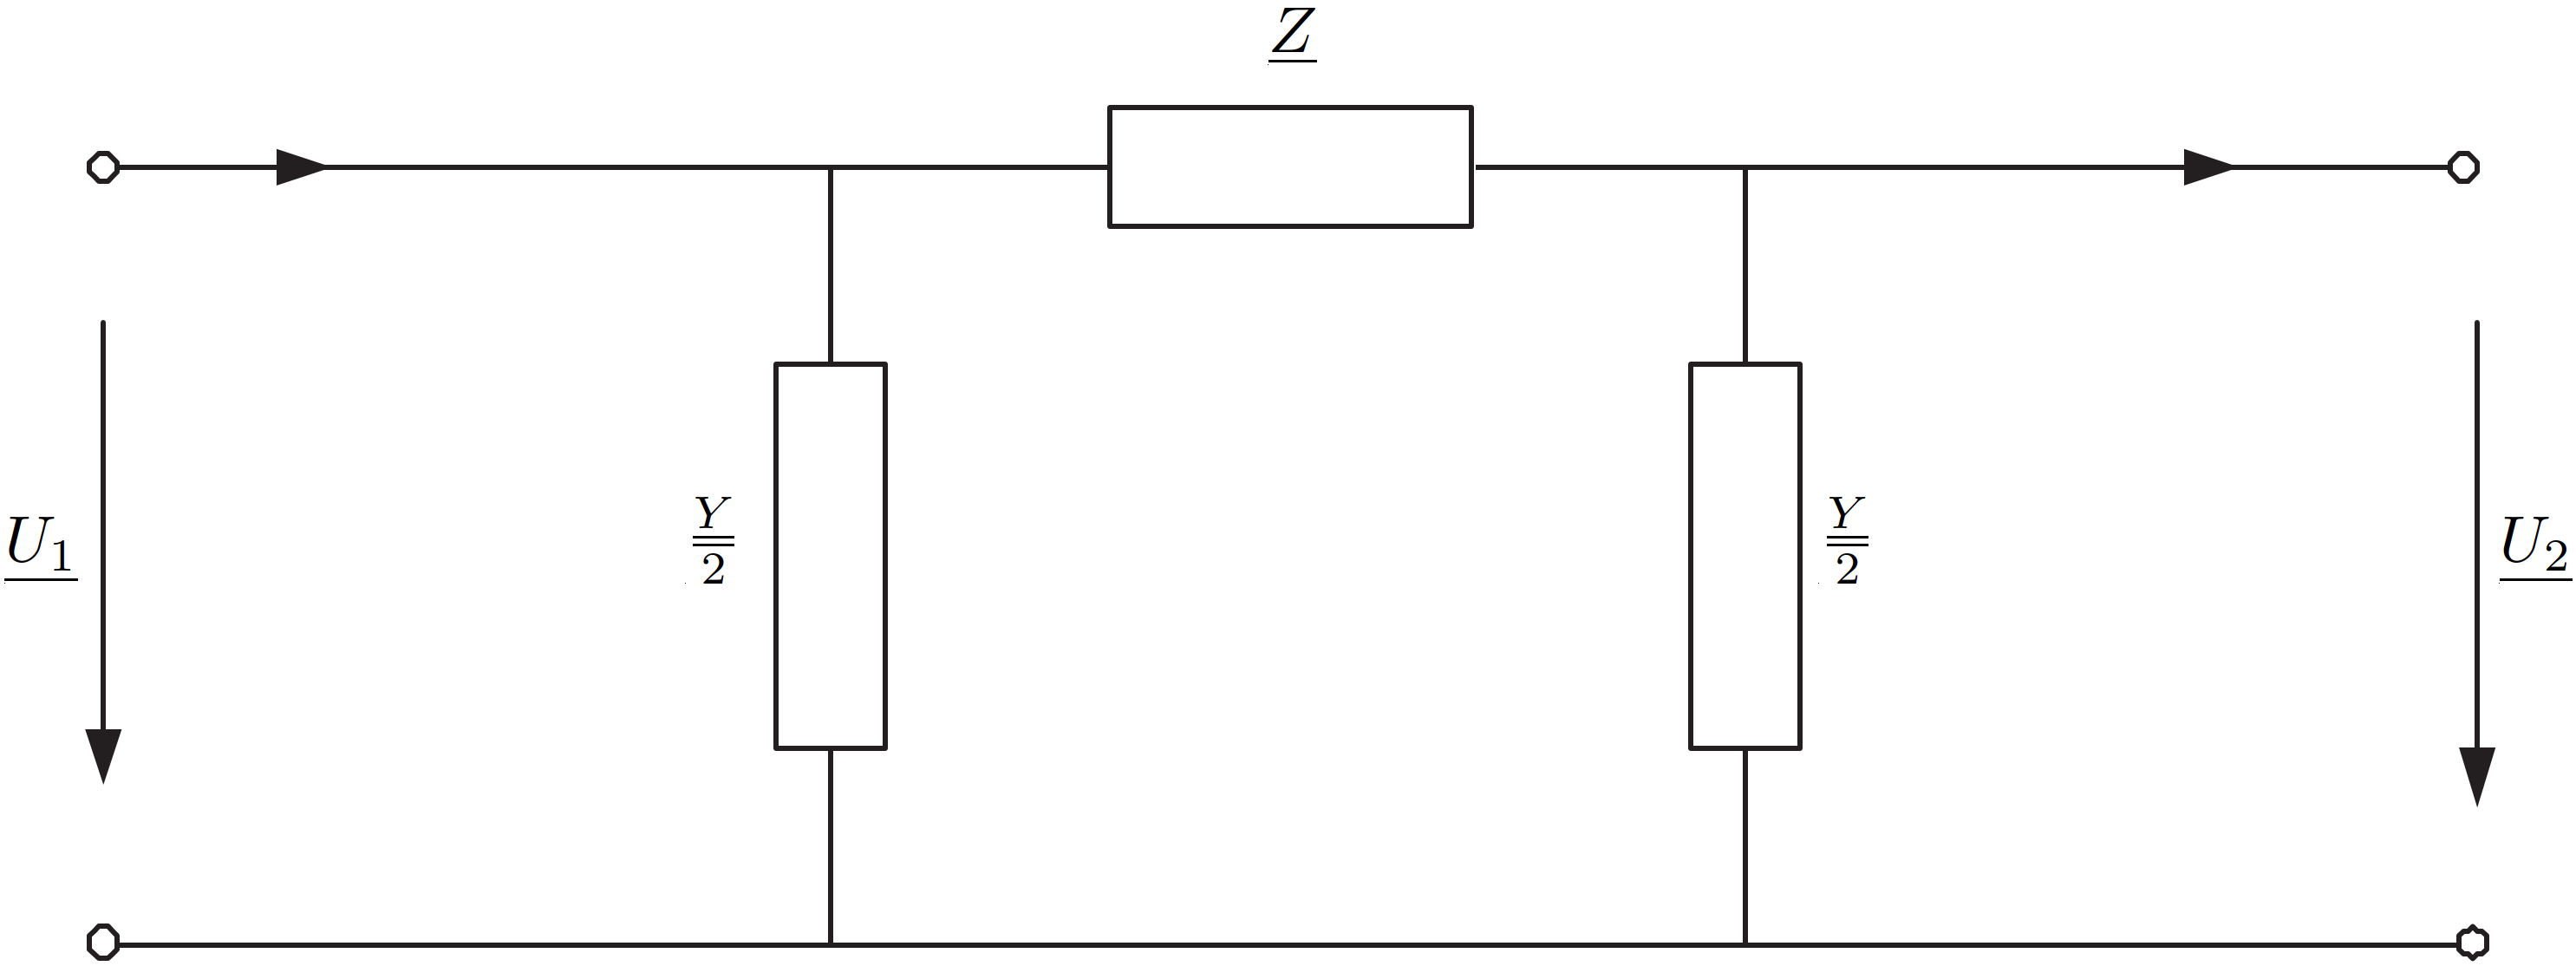
\includegraphics[width=0.9\columnwidth, align=c]{images/Leitungsgleichungen_2.png}
    \end{center}

    \renewcommand{\arraystretch}{1.2}
    $\boxed{
    \begin{pmatrix}
        \underline{U}_1 \\
        \underline{I}_1
    \end{pmatrix}
    =
    \begin{pmatrix}
        1 + \underline{Z} \dfrac{\underline{Y}}{2} & \underline{Z} \\[0.57cm]
        \dfrac{\underline{Y}}{2} \left( 2 + \underline{Z} \dfrac{\underline{Y}}{2} \right) & 1 + \underline{Z} \dfrac{\underline{Y}}{2}
    \end{pmatrix}
    \begin{pmatrix}
        U_2 \\
        \underline{I}_2
    \end{pmatrix}
    }$
    $
    \boxed{
    \frac{|U_2|}{|U_1|} = \left| 
    \frac{
    \displaystyle \frac{1}{\left( \frac{G'}{2} + j \omega \frac{C'}{2} \right) \cdot l}
    }{
    (R' + j \omega L') \cdot l + 
    \displaystyle \frac{1}{\left( \frac{G'}{2} + j \omega \frac{C'}{2} \right) \cdot l}
    }
    \right|
    }$

\subsubsection{Übung Kraftwerk mit Doppelleitung an Netz}
    \begin{minipage}[t]{0.6\columnwidth}
        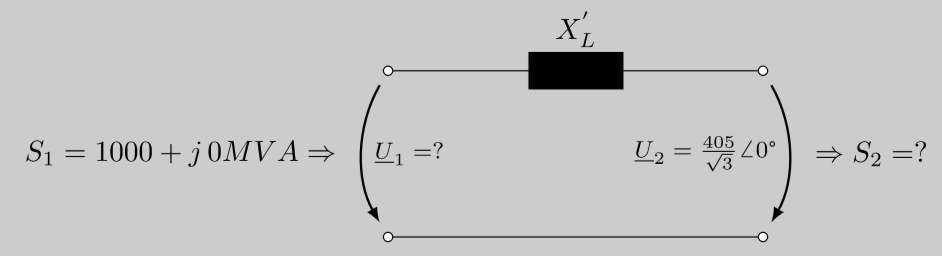
\includegraphics[width=\columnwidth, align=c]{images/u03.png}
    \end{minipage}
    \hfill
    \begin{minipage}[t]{0.39\columnwidth}
        $
        \boxed{
            \underline{U}_1 = \underline{U}_2 + j X'_L \cdot 
            \frac{P_{1,ph} - j Q_{1,ph}}{\underline{U}_1^*}
        }
        $
    \end{minipage} % done
        \section{Betriebsverhalten}
\subsection{Natürliche Leistung}
    \begin{itemize}
        \item Bei einer gewissen Belastung wird in den Querelementen genau so viel Blindleistung „erzeugt“ wie im Längspfad „verbraucht“ wird.
        \item Diese Belastung nennt man natürliche Belastung bzw. natürliche Leistung.
        \item Die Leitung verhält sich neutral bezüglich Blindleistung.
        \item Die natürliche Leistung wird übertragen, wenn die Leitung mit ihrer Wellenimpedanz belastet wird.
    \end{itemize}

    \vspace{0.1cm}

    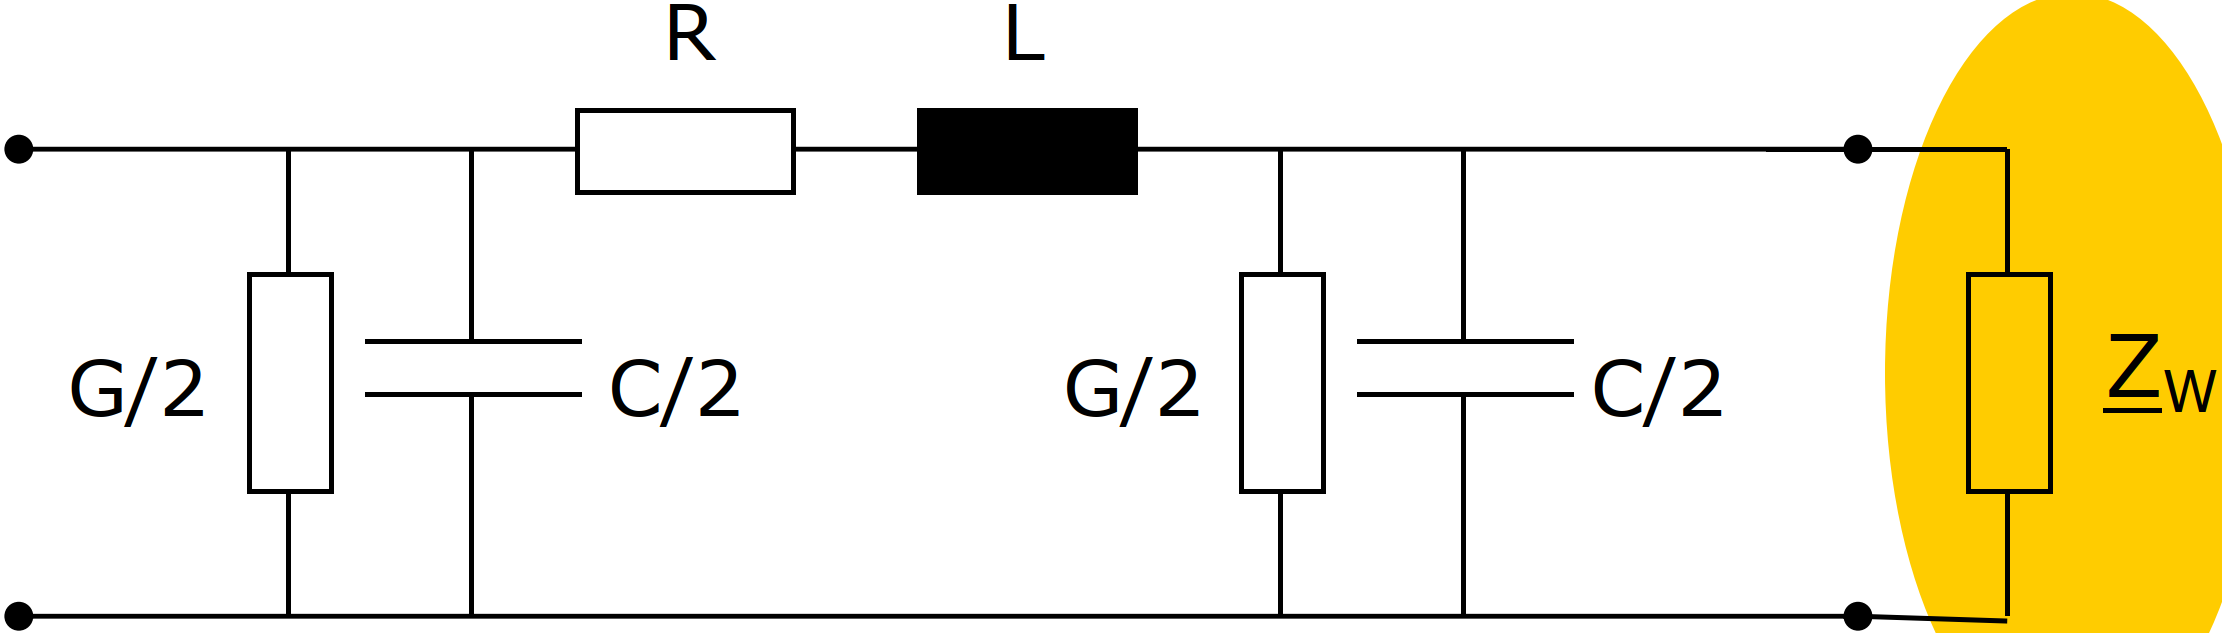
\includegraphics[width=0.9\columnwidth, align=c]{images/Natürliche_Leistung.png}

\subsection{Wellenimpedanz}
    \begin{itemize}
        \item Bei Abschluss mit der Wellenimpedanz „erzeugt“ die Leitung genau so viel Blindleistung wie sie „verbraucht“.
        \item Typische Wellenimpedanzwerte für Freileitung: \( |\!Z_W\!| = 200 \ldots 400\,\Omega \).
        \item Typische Wellenimpedanzwerte für Kabel: \( |\!Z_W\!| = 30 \ldots 50\,\Omega \).
    \end{itemize}

\subsection{Unternatürliche Belastung}
    \begin{itemize}
        \item Die Lastimpedanz ist höher als die Wellenimpedanz.
        \item Die Last nimmt weniger als die natürliche Leistung auf, Leitung nimmt Blindleistung auf.
        \item Die Längsinduktivität „verbraucht“ weniger Blindleistung als die Quer­kapazität „erzeugt“.
        \item Die Spannung am Leitungsende ist höher als am Leitungsanfang.
    \end{itemize}

\subsection{Übernatürliche Belastung}
    \begin{itemize}
        \item Die Lastimpedanz ist niedriger als die Wellenimpedanz.
        \item Die Last nimmt mehr als die natürliche Leistung auf, Leitung gibt Blindleistung ab.
        \item Die Längsinduktivität „verbraucht“ mehr Blindleistung als die Quer­kapazität „erzeugt“.
        \item Die Spannung am Leitungsende ist tiefer als am Leitungsanfang.
    \end{itemize}

\subsection{Praxis}
    \begin{itemize}
        \item \textbf{Kabel} ausschließlich \textbf{unternatürlich} betrieben
        \item \textbf{Freileitungen} meistens \textbf{unternatürlich} betrieben, in seltenen Fällen \textbf{übernatürlich}
    \end{itemize}

\subsection{Leerlauf}
    \begin{minipage}[t]{0.59\columnwidth}
        \begin{itemize}
            \item Extremfall der unternatürlichen Belastung
            \item Leitung verhält sich wie Kapazität
            \item Spannung steigt entlang der Leitung an
            \item Spannungsüberhöhung am Leitungsende 
            \item[] (Ferranti Effekt)
        \end{itemize}
    \end{minipage}%
    \hfill
    \begin{minipage}[t]{0.4\columnwidth}
        % \vspace{0.1cm}
        \centering \vspace{-0.7\baselineskip}
        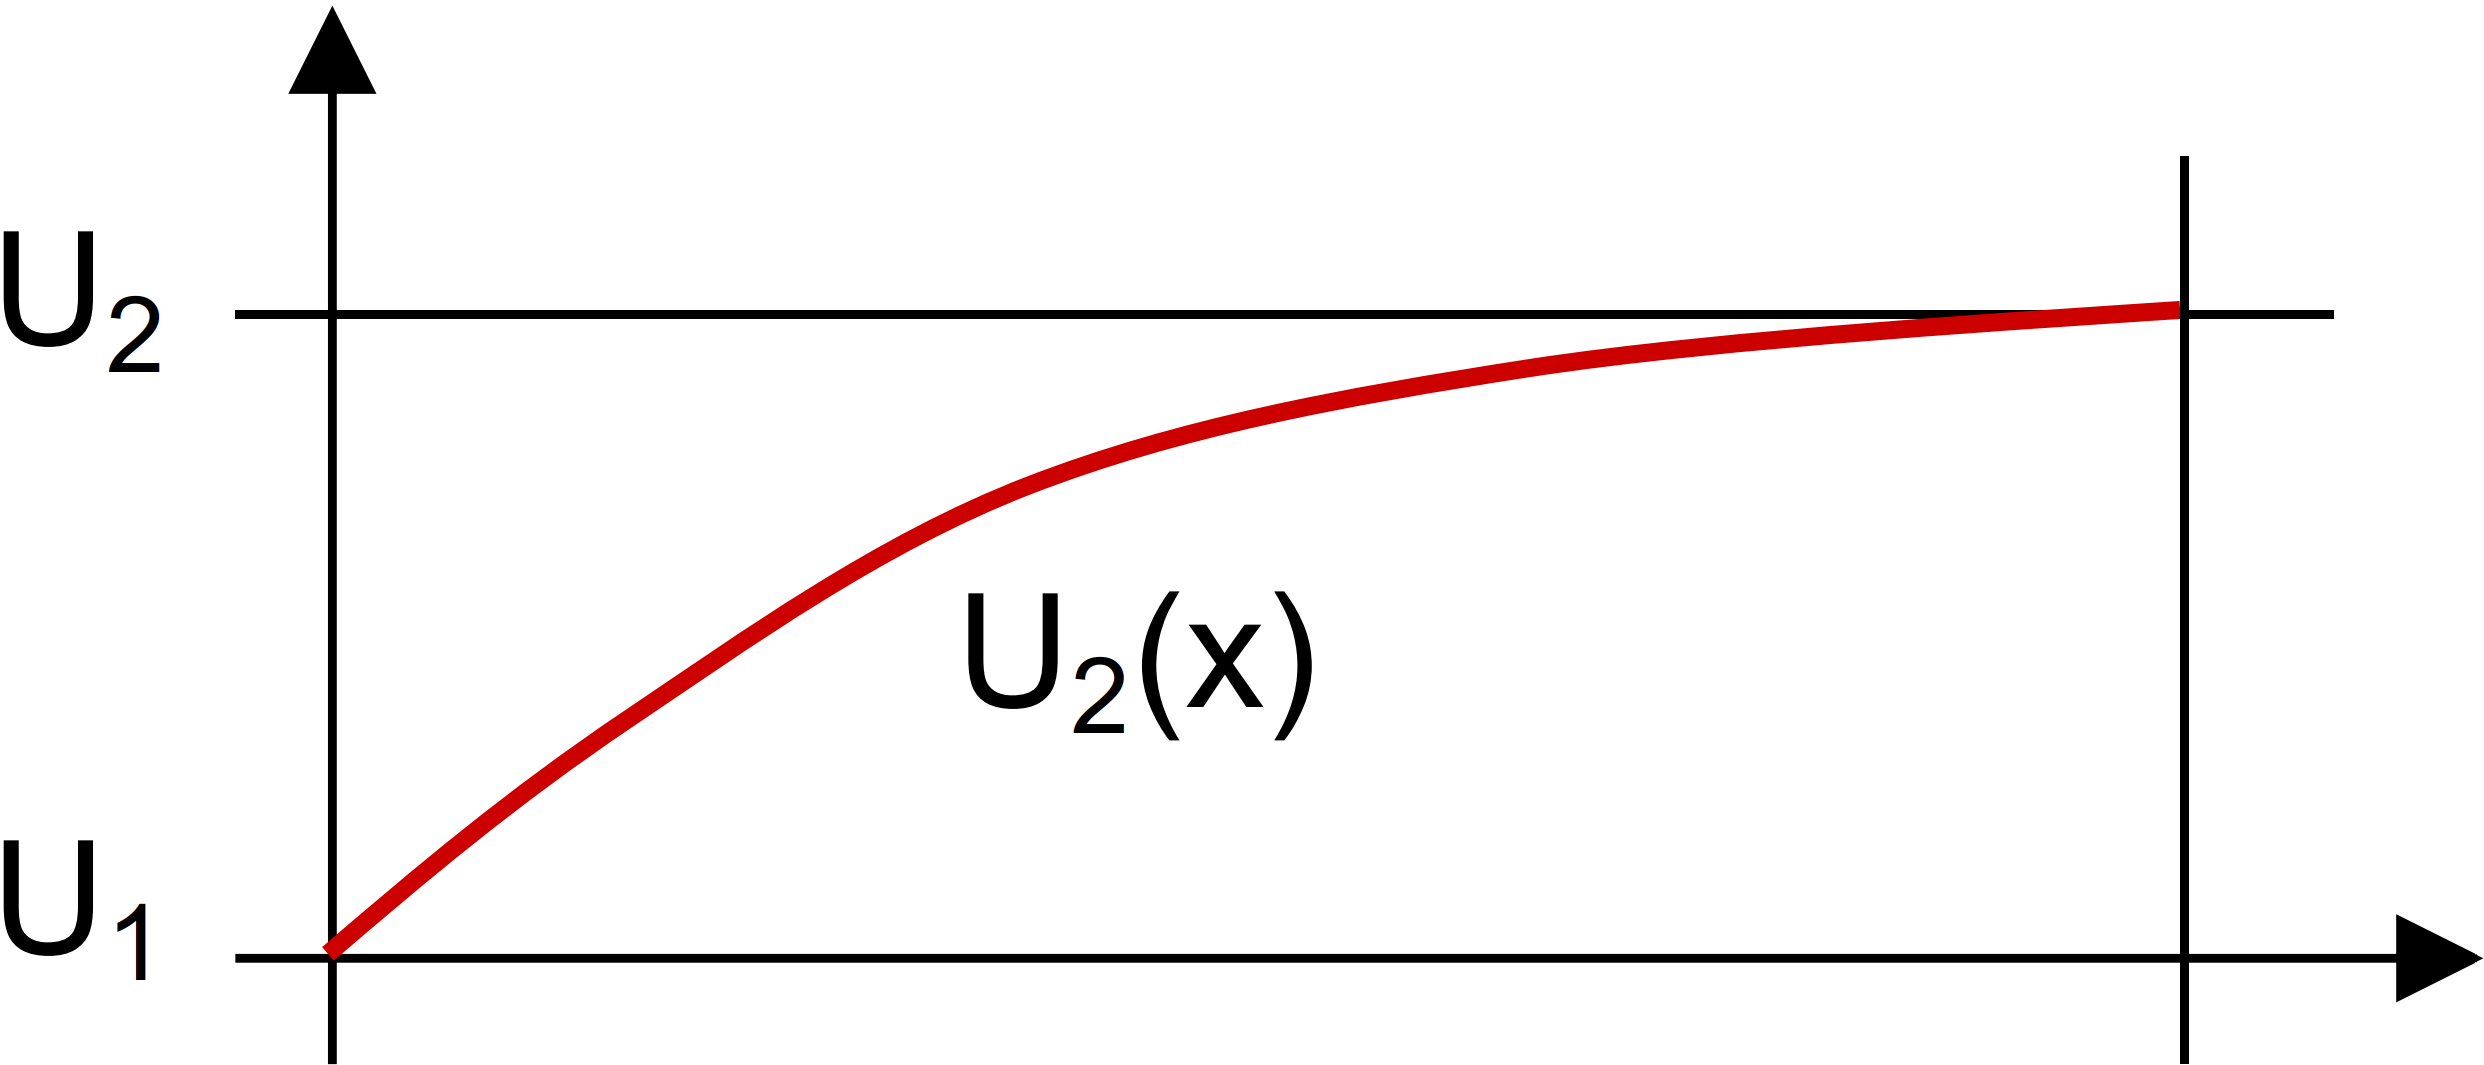
\includegraphics[width=0.9\columnwidth, align=c]{images/Leerlauf.png}
    
        % \vspace{0.1cm}
    \end{minipage}


\subsection{Kurzschluss}
    \begin{itemize}
        \item Extremfall der übernatürlichen Belastung
        \item Leitung verhält sich wie Induktivität
        \item Spannung sinkt entlang der Leitung ab
    \end{itemize}

\subsection{Spannungsabfall entlang einer Leitung}
    \begin{minipage}[t]{0.55\columnwidth}
        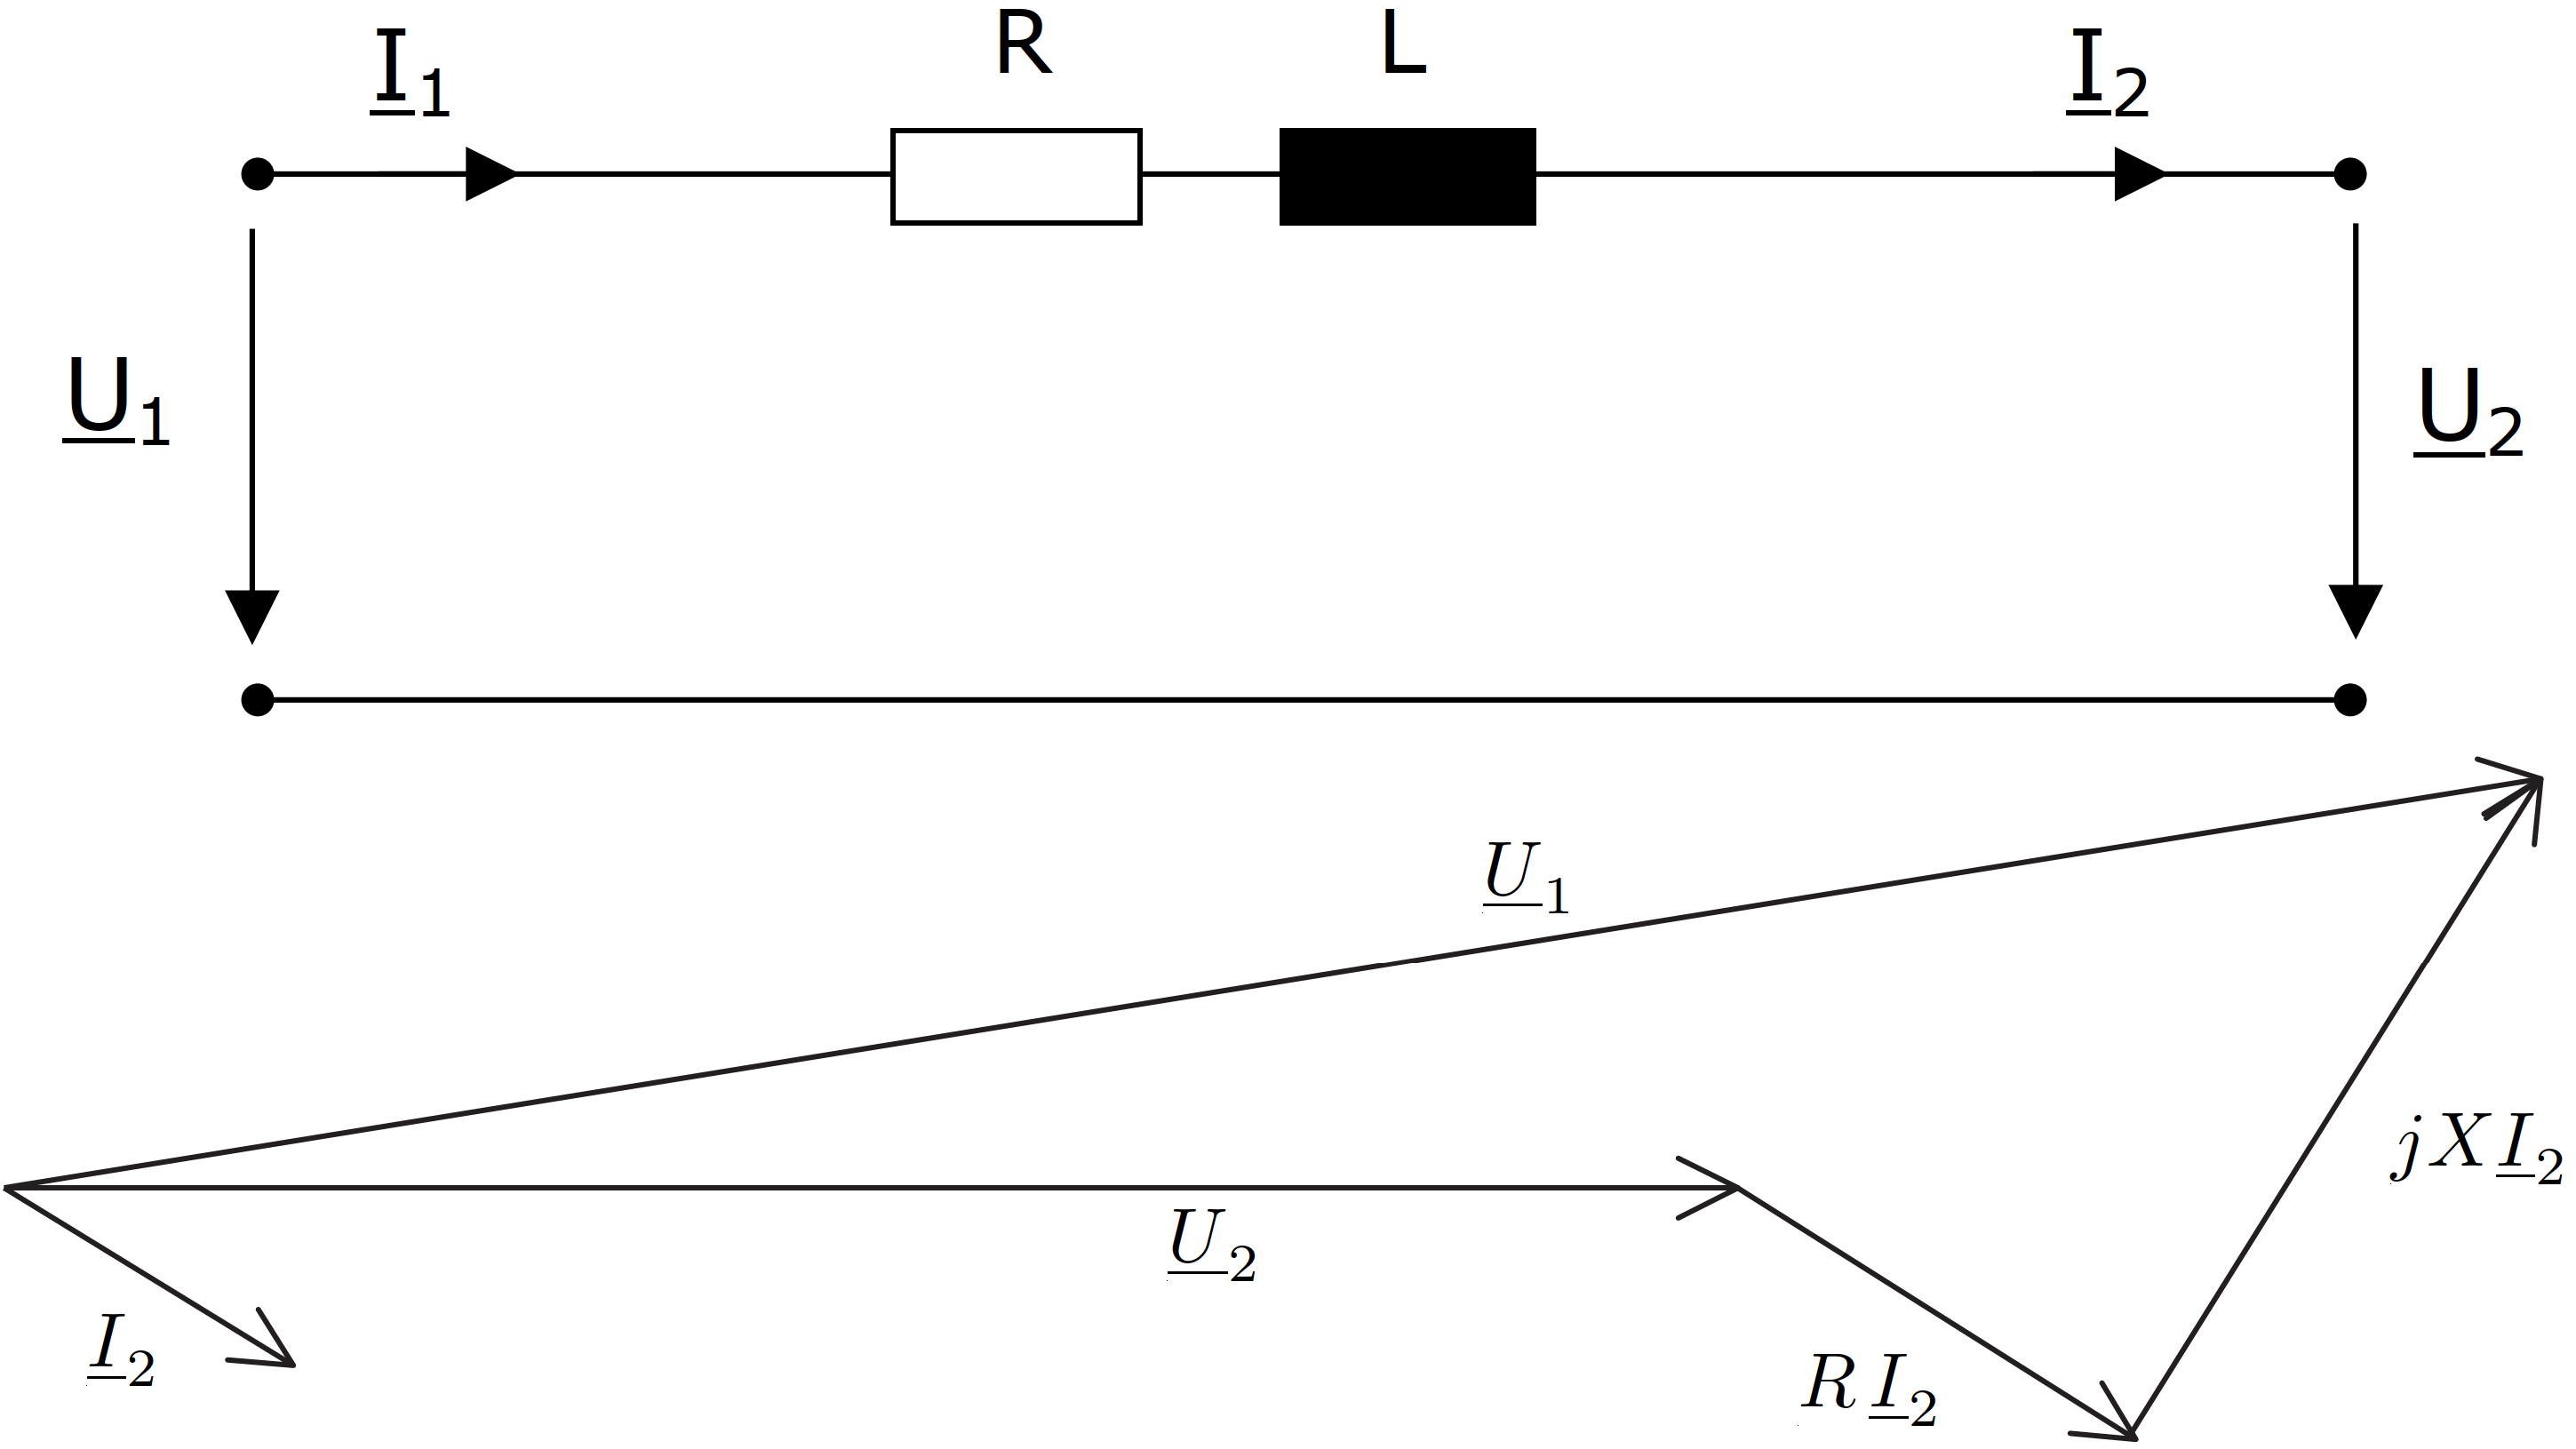
\includegraphics[width=0.95\columnwidth, align=c]{images/Spannungsabfall_entlang_einer_Leitung.png}
    \end{minipage}%
    \hfill
    \begin{minipage}[t]{0.4\columnwidth}
        % \centering \vspace{-0.7\baselineskip}
        \resizebox{!}{0.3\textwidth}{% \begin{figure}[!ht]
% \centering
% \resizebox{1\textwidth}{!}{%
\begin{circuitikz}
\tikzstyle{every node}=[font=\fontsize{18pt}{18pt}\selectfont]
\draw [-{Stealth[scale=1.5]}] (3.75,9) -- (10,9)node[pos=0.5, below, text opacity=1, inner xsep=0.080cm, inner ysep=0.085cm, rounded corners=0.020cm]{$\underline{U}_2$};
\draw [-{Stealth[scale=1.5]}] (10,9) -- (12.5,7.75)node[pos=0.5, below, text opacity=1, inner xsep=0.080cm, inner ysep=0.085cm, rounded corners=0.020cm]{$R\underline{I}_2$};
\draw [-{Stealth[scale=1.5]}] (3.75,9) -- (5,8.375)node[pos=0.5, below, text opacity=1, inner xsep=0.080cm, inner ysep=0.085cm, rounded corners=0.020cm]{$\underline{I}_2$};
\draw [-{Stealth[scale=1.5]}] (12.5,7.75) -- (14.25,11.375)node[pos=0.5, right, text opacity=1, inner xsep=0.080cm, inner ysep=0.085cm, rounded corners=0.020cm]{$jX\underline{I}_2$};
\draw [-{Stealth[scale=1.5]}] (3.75,9) -- (14.25,11.375)node[pos=0.5, above, text opacity=1, inner xsep=0.080cm, inner ysep=0.085cm, rounded corners=0.020cm]{$\underline{U}_1$};
\end{circuitikz}
% }%
% \caption{Your Caption}
% \label{fig:my_label}
% \end{figure}\unskip}
    \end{minipage}


\subsubsection{Phasenstrom durch Leitung}
    $
    \boxed{
    I_{Phase} = \frac{U_{Phase}}{Z_{Phase}}
    }
    $

    \vspace{0.1cm} % done
        \input{sections/58_Transformatormodell.tex} % done
        \section{Leistungsfluss über eine Leitung}
\subsubsection{Mathematische Vereinfachungen im Voraus}
    \begin{minipage}[c]{0.48\columnwidth}
            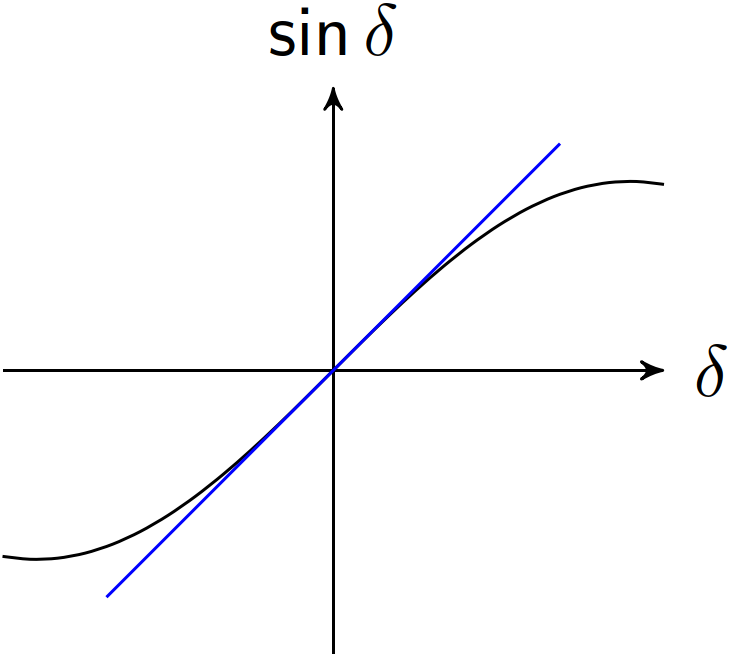
\includegraphics[width=0.7\textwidth, align=c]{images/Erkenntnisse_1.png}

            \begin{itemize}
                \item für kleinere Winkel: $\sin\delta \approx \delta$
                \item Maximale Steigung
            \end{itemize}    
    \end{minipage}
    \hfill
    \begin{minipage}[c]{0.48\columnwidth}
            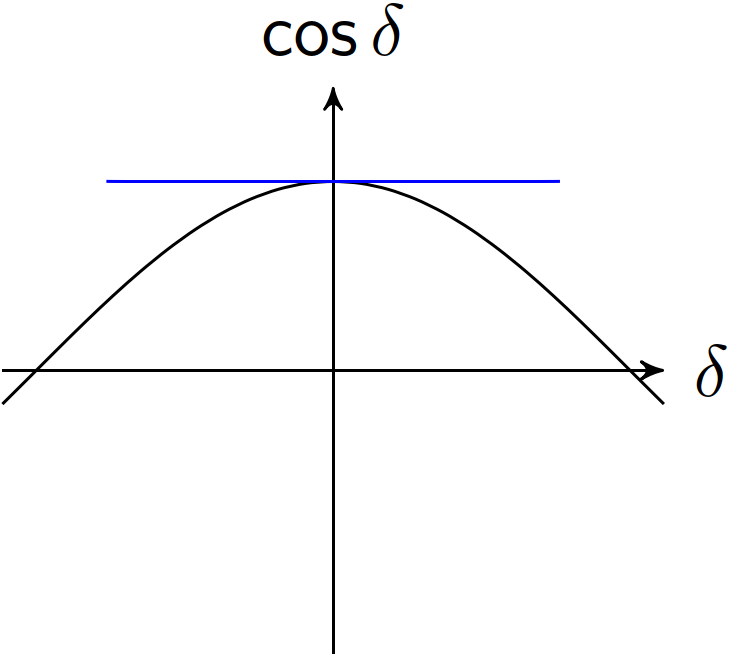
\includegraphics[width=0.7\textwidth, align=c]{images/Erkenntnisse_2.png}

            \begin{itemize}
                \item für kleinere Winkel: $\cos\delta \approx 1$
                \item Minimale Steigung
            \end{itemize}
    \end{minipage}

\subsection{Leistungsfluss}
    \begin{minipage}[t]{0.6\columnwidth}
        \centering \vspace{-0.7\baselineskip}
        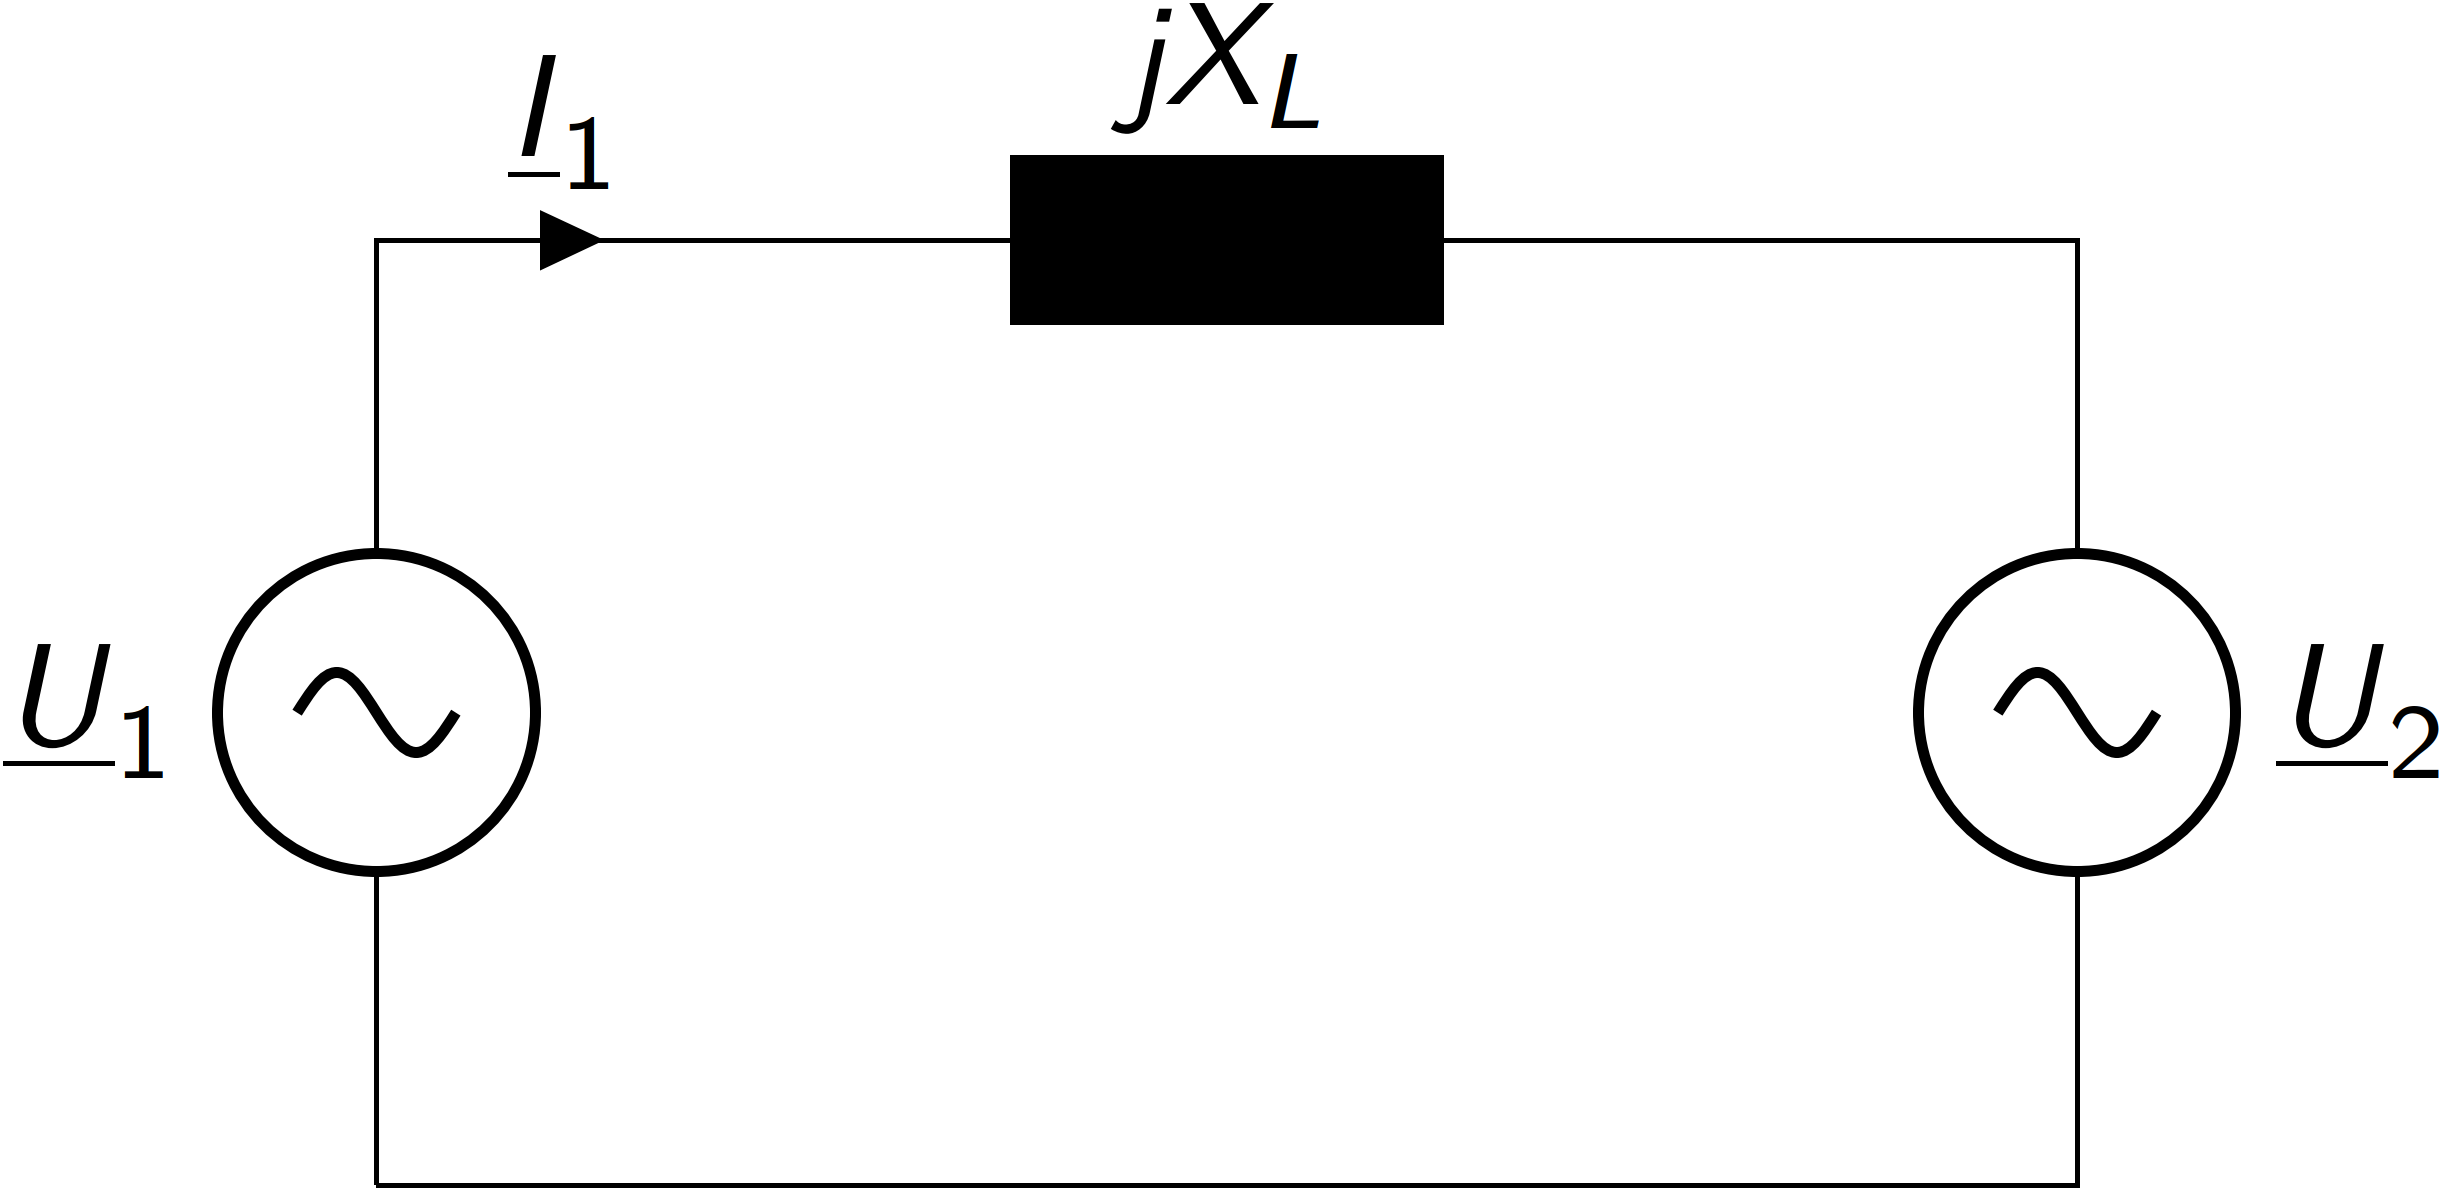
\includegraphics[width=0.85\linewidth]{images/Leistungsübertragung_1.png}
    \end{minipage}%
    \hfill
    \begin{minipage}[t]{0.39\columnwidth}
        \begin{itemize}
            \item Verlustlose Leitung
            \item Ideale Spannungsquellen $\underline{U}_1$ und $\underline{U}_2$
        \end{itemize}
    \end{minipage}

\subsection{Leistungsübertragung}
    $\boxed{\underline{U}_1 = U_1 \cdot e^{j \cdot \theta_1}} \quad \boxed{\underline{U}_2 = U_2 \cdot e^{j \cdot \theta_2}}$
    $\quad$
    $\boxed{X_L = \omega \cdot L = \omega \cdot L' \cdot l} \quad \boxed{\omega = 2 \cdot \pi \cdot f}$

    \vspace{0.1cm}

    % $\boxed{\underline{I}_1 = \frac{U_1 - U_2}{j \cdot X_L} = \frac{U_1 \cdot e^{j \cdot \theta_1} - U_2 \cdot e^{j \cdot \theta_2}}{j \cdot X_L}} \quad $

    $\boxed{\underline{I}_1^* = \frac{U_1 \cdot e^{-j \cdot \theta_1} - U_2 \cdot e^{-j \cdot \theta_2}}{-j \cdot X_L}
    = \frac{j}{X_L} \left( U_1 \cdot e^{-j \cdot \theta_1} - U_2 \cdot e^{-j \cdot \theta_2} \right)}$

    \vspace{0.1cm}

    $\boxed{\delta = \theta_1 - \theta_2}$
    $\boxed{\underline{S}_1 = \underline{U}_1 \cdot \underline{I}_1^* = {P}_1 + j \cdot {Q}_1}$

    $\boxed{
    \underline{S}_1 = \underbrace{U_1 \cdot U_2 \cdot \frac{1}{X_L} \cdot \sin(\delta)}_{P_1}
    + j\, \underbrace{\left( U_1^2 \cdot \frac{1}{X_L} - U_1 \cdot U_2 \cdot \frac{1}{X_L} \cos(\delta) \right)}_{Q_1}}$

    \vspace{0.1cm}

    $\boxed{P_1 = \text{Re}\left\{ \underline{U}_1 \cdot \underline{I}_1^*\right\}= U_1 \cdot U_2 \cdot \frac{1}{X_L} \cdot \sin(\delta)}$

    \vspace{0.1cm}

    $\boxed{Q_1 = \text{Im}\left\{ \underline{U}_1 \cdot \underline{I}_1^*\right\} = U_1^2 \cdot \frac{1}{X_L} - U_1 \cdot U_2 \cdot \frac{1}{X_L} \cos(\delta)}$

    \renewcommand{\arraystretch}{1.2}
    \begin{tabular}{@{} l p{6cm} l @{}}
    $U_1$        & Effektive Spannungen am Leitungsanfang \dotfill & $\mathrm{V}$ \\
    $U_2$        & Effektive Spannungen am Leitungsende \dotfill & $\mathrm{V}$ \\
    $\theta_1$ & Phasenwinkel der Spannungen am Leitungsanfang \dotfill & $\mathrm{rad}$ \\
    $\theta_2$ & Phasenwinkel der Spannungen am Leitungsende \dotfill & $\mathrm{rad}$ \\
    % $j$                 & Imaginäre Einheit ($j^2 = -1$) \dotfill & $-$ \\
    $\omega$            & Kreisfrequenz \dotfill & $\mathrm{rad/s}$ \\
    $f$                 & Netzfrequenz \dotfill & $\mathrm{Hz}$ \\
    $L$                 & Induktivität der Leitung \dotfill & $\mathrm{H}$ \\
    $L'$                & Induktivität pro Längeneinheit \dotfill & $\mathrm{H/m}$ \\
    $l$                 & Leitungslänge \dotfill & $\mathrm{m}$ \\
    $X_L$               & Reaktanz der Leitung  \dotfill & $\Omega$ \\
    % $I_1$               & Strom am Leitungsanfang \dotfill & $\mathrm{A}$ \\
    $I_1^*$             & Komplex konjugierter Strom \dotfill & $\mathrm{A}$ \\
    $S_1$               & Scheinleistung am Leitungsanfang \dotfill & $\mathrm{VA}$ \\
    $P_1$               & Wirkleistung \dotfill & $\mathrm{W}$ \\
    $Q_1$               & Blindleistung \dotfill & $\mathrm{VAR}$ \\
    $\delta$           & Phasendifferenz \dotfill & $\mathrm{rad}$ \\
    \end{tabular}

\subsection{Praxis (Vereinfachung)}\label{Leistungsübertragung}
    $U_1 \approx U_2$, $\delta$ in der Regel klein, $\delta \leq 40^\circ$

    % \vspace{0.1cm}
    Mit den Vereinfachungen (Anfangs Kapitel) und den aufgeführten Punkten ergibt sich:
    % \vspace{0.1cm}

    $\boxed{P_{12} = \frac{U_1 U_2}{X} \sin(\delta_{12})}$
    $\boxed{Q_{12} = \frac{U_1^2 - U_1 U_2 \cdot \cos(\delta_{12})}{X}}$
    $\boxed{Q_{21} = \frac{U_2^2 - U_2 U_1 \cdot \cos(-\delta_{12})}{X}}$

\subsubsection{Erkenntisse für Wirk- und Blindleistung}
    \begin{minipage}[t]{0.49\columnwidth}
        \textbf{Wirkleistung:}

        \begin{itemize}
            \item \textbf{Stark} abh. von der Phasendifferenz $\delta$
            \item \textbf{Wenig} abh. vom Spannungsbetrag $U_1, U_2$
        \end{itemize}
    \end{minipage}%
    \hfill
    \begin{minipage}[t]{0.49\columnwidth}
        \textbf{Blindleistung:}

        \begin{itemize}
            \item \textbf{Stark} abh. von der Phasendifferenz $\delta$
            \item \textbf{Wenig} abh. vom Spannungsbetrag $U_1, U_2$
        \end{itemize}
    \end{minipage}

\subsection{Maximale Wirkleistungsübertragung}
    \begin{minipage}[c]{0.35\columnwidth}
        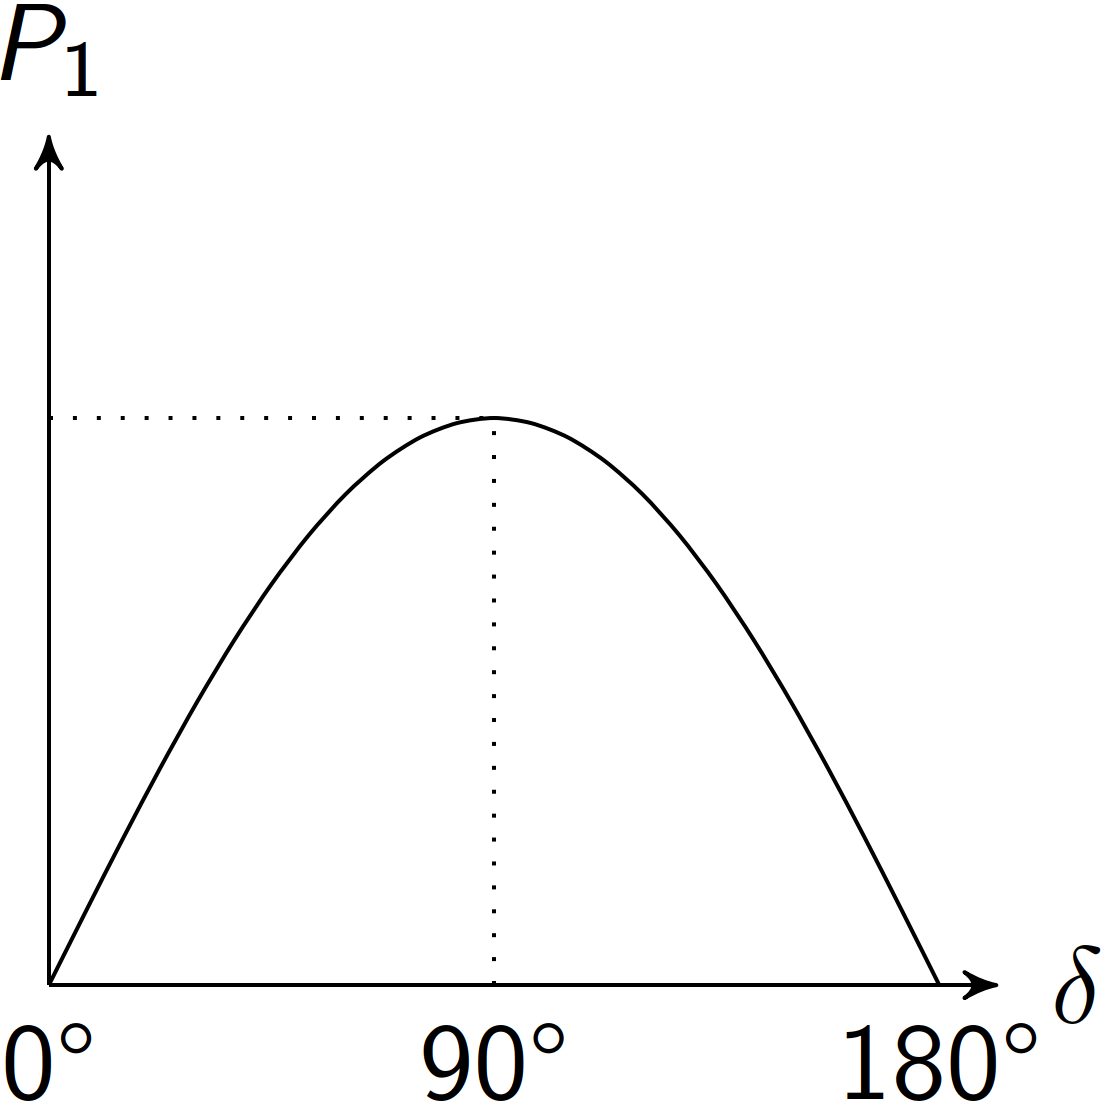
\includegraphics[width=0.7\textwidth]{images/Maximale_Wirkleistungsübertragung.png}
    \end{minipage}
    \hfill
    \begin{minipage}[c]{0.48\columnwidth}
        $\boxed{P_{1_{\text{max}}}^{1ph} = \frac{U_1 \cdot U_2}{X_{12}}}$

        $\boxed{P_{1_{\text{max}}} = 3\frac{U_1 \cdot U_2}{X_{12}}}$
    \end{minipage} % done
        \input{sections/61_Lastflussproblem.tex} % done
        \newcolumn
\section{Störungen in Stromnetzen}
\subsection{Normaler Betriebszustand}
  \begin{minipage}[t]{0.59\columnwidth}
      \begin{itemize}
        \item Spannungen und Ströme im zulässigen Bereich
        \item Intakter Isolationszustand
    \end{itemize}
  \end{minipage}%
  \hfill
  \begin{minipage}[t]{0.4\columnwidth}
      \begin{itemize}
        \item Intakte Betriebsmittel
        \item Gewünschter Schaltzustand
    \end{itemize}
  \end{minipage}

\subsection{Definitionen: Fehler, Störung, Schaden}
  \begin{itemize}
    \item \textbf{Fehler:} Ungewollte Änderung des normalen Betriebszustandes
    \item \textbf{Störung:} Folge eines Fehlers, umfasst gesamten Ablauf vom Fehlereintritt bis zur Beseitigung; kann Versorgungsunterbrechung mit sich ziehen
    \item \textbf{Schaden:} Bleibende, nachteilige Veränderung an einem Betriebsmittel
  \end{itemize}

\subsection{Fehlerarten}
  \begin{center}
    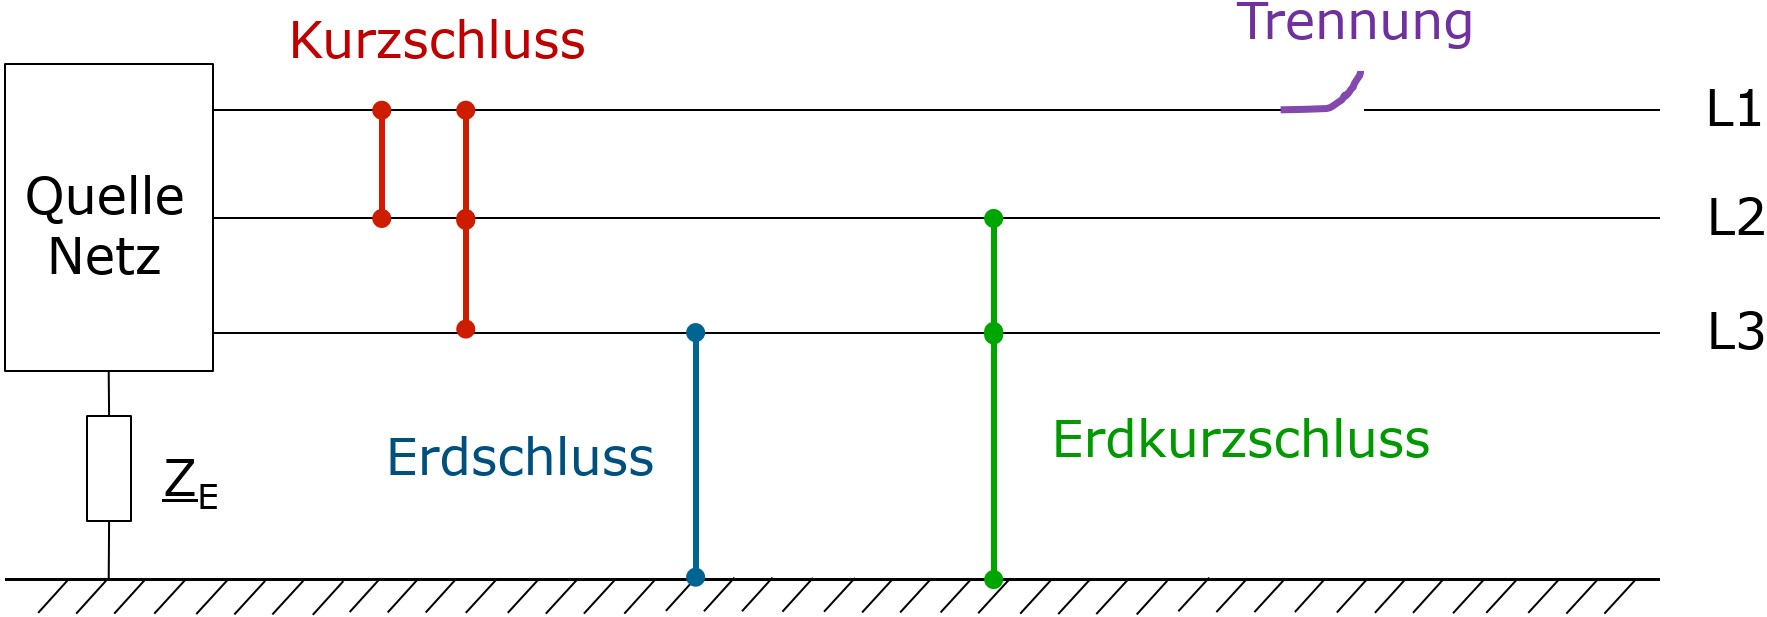
\includegraphics[width=0.8\columnwidth]{images/Fehlerarten_1.jpg}
  \end{center}

  \vspace{-0.4cm}

  \begin{minipage}[t]{0.49\columnwidth}
    \subsubsection{Niederohmige Fehler}
      „Satter” Kurzschluss, sehr gut leitende Verbindung zwischen Phasen und/oder Erde, \textbf{hoher Fehlerstrom}
  \end{minipage}%
  \hfill
  \begin{minipage}[t]{0.49\columnwidth}
    \subsubsection{Hochohmiger Fehler}
      Schlecht leitende Verbindung zwischen Phasen und/oder Erde, \textbf{geringer Fehlerstrom}
  \end{minipage}

  \begin{minipage}[t]{0.49\columnwidth}
    \subsubsection{Symmetrischer Fehler}
      \begin{itemize}
        \item Gleicher Fehler in allen drei Phasen
        \item Dreiphasiger (Erd-)Kurzschluss
        \item Dreiphasige Unterbrechung
      \end{itemize}
  \end{minipage}%
  \hfill
  \begin{minipage}[t]{0.49\columnwidth}
    \subsubsection{Unsymmetrische Fehler}
      \begin{itemize}
        \item Ein- und zweiphasige (Erd-)Kurzschlüsse
        \item Ein- und zweiphasige Unterbrechungen
      \end{itemize}
  \end{minipage}

\subsection{Sternpunktbehandlung}
  \textbf{Wichtigkeit:} Der Schutztechnik wird die Art der Sternpunktbehandlung vorgegeben. Alle Schutzsysteme sind dahingehend auszuwählen und entsprechend einzustellen.

  \begin{minipage}[t]{0.65\columnwidth}
      \centering \vspace{-0.7\baselineskip}
      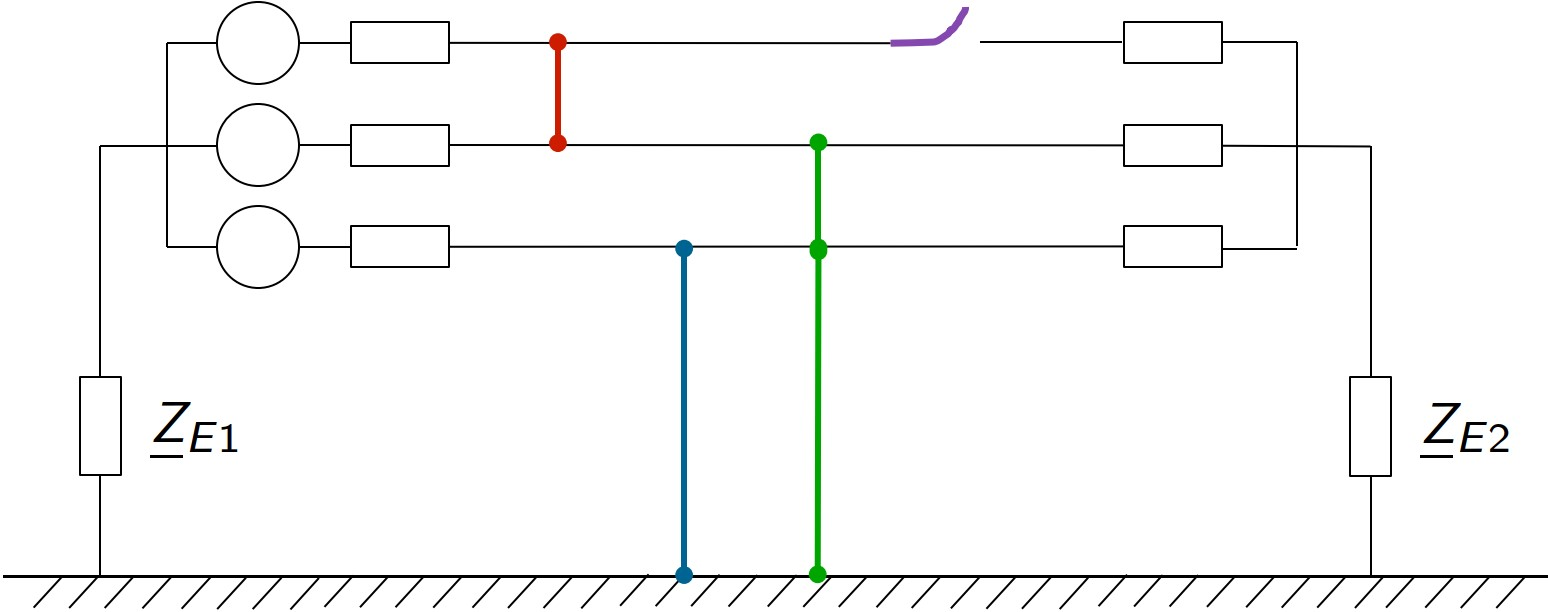
\includegraphics[width=0.95\linewidth]{images/Sternpunktbehandlung_1.jpg}
  \end{minipage}%
  \hfill
  \begin{minipage}[t]{0.34\columnwidth}
    \begin{itemize}
      \item $Z_E = 0$: „starre” Erdung
      \item $Z_E$ klein: 
      \item[] niederohmige Erdung
      \item $Z_E$ gross: 
      \item[] hochohmige Erdung
    \end{itemize}
  \end{minipage}


\subsubsection{Sternpunktverschiebung (einpoliger Unterbruch)}
  \begin{minipage}[c]{0.78\columnwidth}
      %\begin{center}
          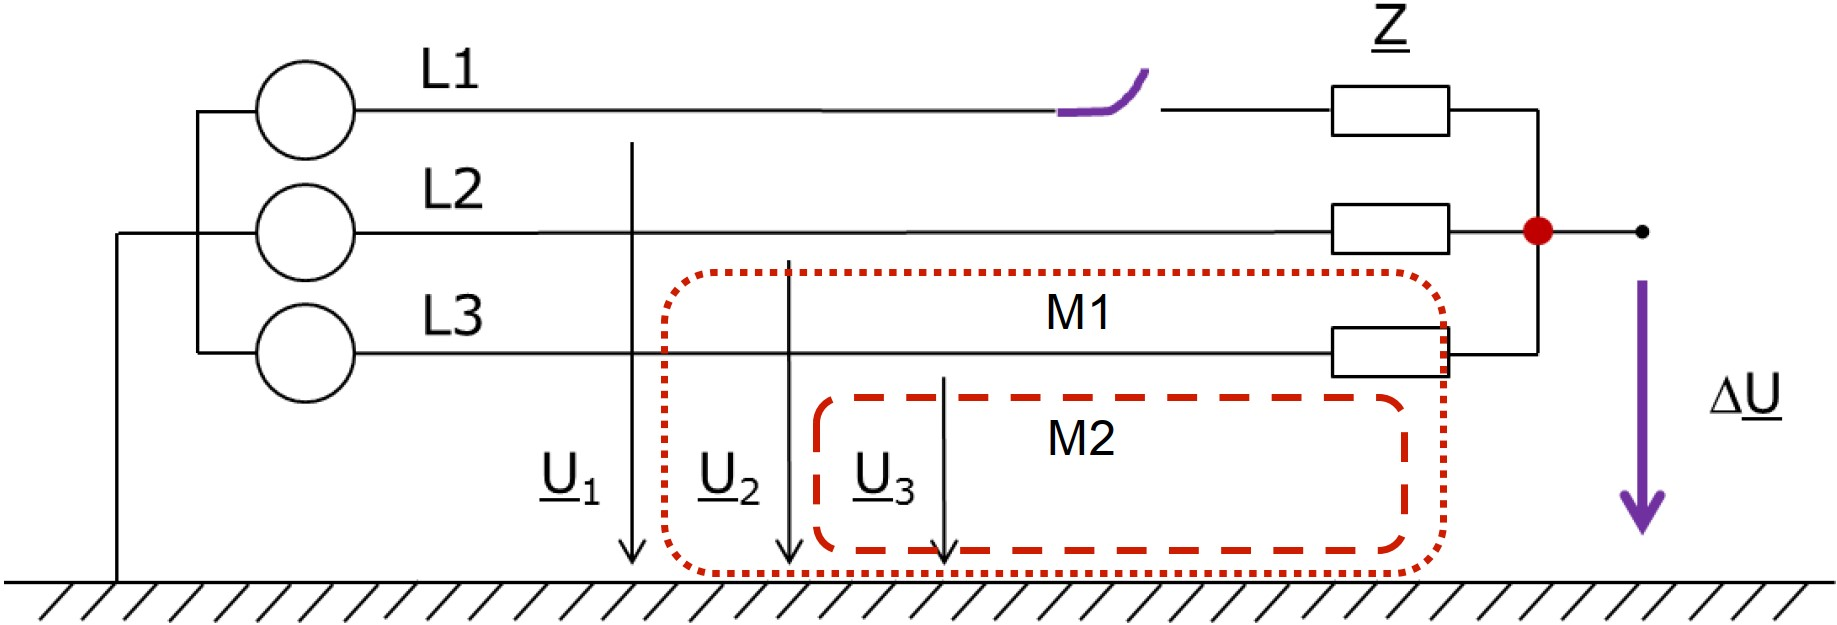
\includegraphics[width=0.98\columnwidth, align=c]{images/Sternpunktverschiebung_1.jpg}
      %\end{center}    
  \end{minipage}
  \hfill
  \begin{minipage}[c]{0.2\columnwidth}
      %\begin{center}
          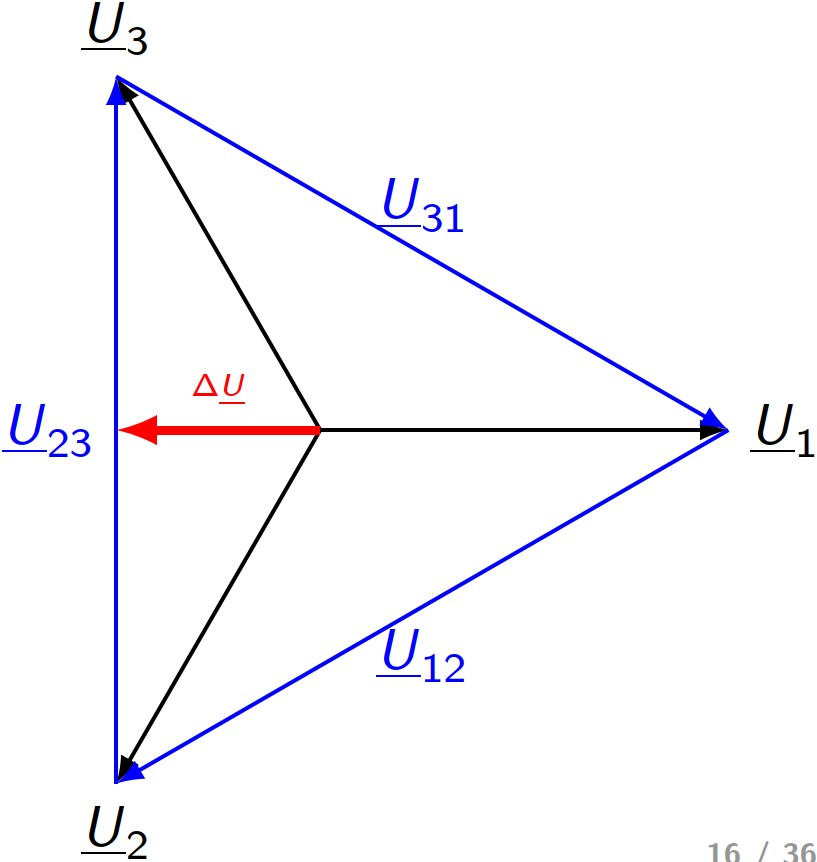
\includegraphics[width=0.98\columnwidth, align=c]{images/Sternpunktverschiebung_2.jpg}
      %\end{center} 
  \end{minipage}

  \textbf{Herleitung:}
  \begin{enumerate}
    \item Nach Unterbrechung von L1 fliesst in L2 und L3 der Strom $I_{23}$. \\
          Er verursacht einen entsprechenden Spannungsabfall an der Impedanz $\underline{Z}$.
    \item Aufstellen der Gleichung für Masche M1 und Berechnung $\Delta \underline{U}$.
    \item Aufstellen der Gleichung für Masche M2 und Berechnung $\Delta \underline{U}$.
    \item Addieren Sie die Ergebnisse aus 2. und 3. und berechnen Sie daraus $\Delta \underline{U}$.
  \end{enumerate}

  \begin{minipage}[t]{0.4\columnwidth}
    \centering \vspace{-0.7\baselineskip}
    $\Delta \underline{U} = \underline{U_2} - \underline{I_{23}} \underline{Z} = \underline{U_3} + \underline{I_{23}} \underline{Z} $
  
    $2 \cdot \Delta \underline{U} = \underline{U_2} + \underline{U_3}$
  \end{minipage}%
  \begin{minipage}[t]{0.4\columnwidth}
    \centering \vspace{-0.7\baselineskip}
    \textbf{\crd{Wichtig:}}
    $\boxed{\Delta \underline{U} = \frac{\underline{U_2} + \underline{U_3}}{2}}$
    
  \end{minipage}

  $\Delta \underline{U}$ ist unabhängig von $\underline{Z}$, da wir ein symmetrisches System haben ($\underline{Z}_1 = \underline{Z}_2 = \underline{Z}_3$).



\subsection{\texorpdfstring{Sternpunktspannung 2 (Störimpedanz $\Delta$ Z beigefügt)}{Sternpunktspannung 2 (Störimpedanz Delta Z beigefügt)}}
  \begin{minipage}[c]{0.48\columnwidth}
      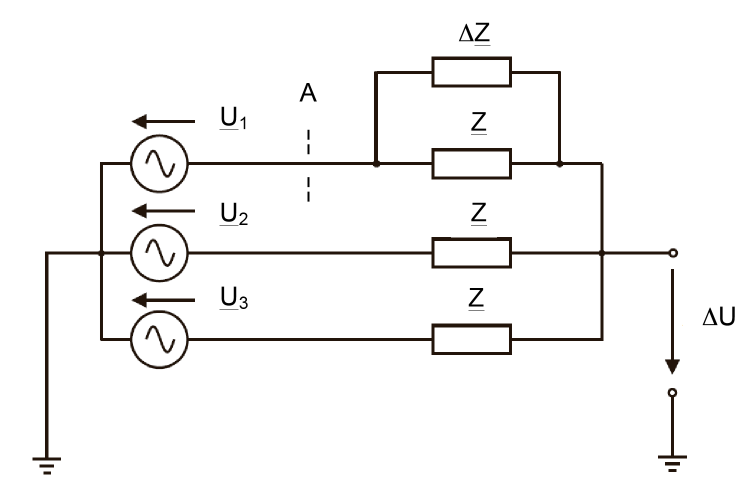
\includegraphics[width=\columnwidth, align=c]{images/u04.png}
  \end{minipage}
  \hfill
  \begin{minipage}[c]{0.4\columnwidth}
      $\boxed{
          \Delta \underline{U} = \frac{
          \underline{U_1} \left(1 + \frac{Z}{\Delta Z} \right) + \underline{U_2} + \underline{U_3}
          }{
          3 + \frac{Z}{\Delta Z}
          }}$
  \end{minipage}

\section{Leittechnik}
\subsection{Ruhestromauslösung}
\begin{tabular}{ll}
  \textbf{Funktion:}        & Löst bei Erreichen eines Schwellwerts aus, \\
                            & kein Strom im Normalzustand \\
  \textbf{\cgn{Vorteil:}}   & Einfache \& zuverlässige Überstromdetektion, \\
                            & direkte Auslösung bei Grenzwerten \\
  \textbf{\crd{Nachteil:}}  & Benötigt externe Energiequelle für Auslösung, \\
                            & im Gegensatz zur Ruhespannungsauslösung \\
\end{tabular}
% Funktion: Die Ruhestromauslösung (auch Arbeitsstromauslösung) ist ein Schutzprinzip, bei dem ein Auslösekriterium (z.B. ein Stromfluss in einem überwachten Kreis) beim Erreichen eines Schwellenwerts die Auslösung eines Schalters bewirkt. Im Normalzustand fliesst kein Strom im Auslösekreis, bei einem Fehler jedoch schon, wodurch der Schutz ausgelöst wird. \\
% Beispiel aus der Kraftwerkstechnik: \\
% Überstromauslösung eines Generatorschutzrelais: Wenn der Strom im Generator einen bestimmten Grenzwert überschreitet (z.B. bei einem Kurzschluss), wird ein Signal an den Leistungsschalter gesendet, um den Generator vom Netz zu trennen.\\
% Vorteil: Einfache und zuverlässige Detektion von Überströmen oder anderen Fehlerzuständen.  Direkte Auslösung bei Erreichen des Grenzwertes. \\
% Nachteile: Benötigt eine externe Energiequelle für den Auslösemechanismus. Bei Ausfall dieser Energiequelle (z.B. Hilfsspannung) ist der Schutz unwirksam. Dies im Gegensatz zur Ruhespannungsauslösung.  % done
        \section{Schutztechnik}
\subsection{Aufgaben der Schutztechnik}
    \begin{itemize}
    \item Gewährleistung der Kontinuität des Betriebs und die Stabilität des Netzes
    \item \textbf{Sicheres, schnelles} und \textbf{selektives} Abschalten der gestörten Netzelemente
    \item Schutzsystem muss die Fähigkeit haben, den \textbf{Fehlerzustand} vom \textbf{normalen Betriebszustand} genau zu unterscheiden.
    \item Einleitung von \textbf{Massnahmen}, die sich möglichst eng begrenzt \textbf{auf den Fehlerort} beziehen
    \end{itemize}

\subsection{Selektivität}
    \begin{itemize}
    \item Selektivität gewährleistet, dass im Fehlerfall möglichst nur der fehlerhafte Netzabschnitt oder Verbraucher abgeschaltet wird und andere Netzabschnitte und Verbraucher nicht mit beeinträchtigt werden.
    \item Erreichen durch \textbf{Staffelung}
    \begin{itemize}
        \item Zeitstaffelung
        \item Stromstaffelung
        \item Impedanzstaffelung
    \end{itemize}
    \item zeitverkürzte Selektivität erzielen:
    Die zeitverkürzte Selektivitäts-Steuerung (ZSS) nutzt eine Kommunikation zwischen den Leistungsschaltern, um unnötige Verzögerungen zu vermeiden.
    \end{itemize}

\subsection{Überstrom-Zeit-Schutz}
    Die Auswertung der Stromamplitude ist die einfachste Methode den normalen Betriebszustand eines Netzes von einem Netzfehler zu unterscheiden.

    % \vspace{0.1cm}

    \textbf{Anwendung:} Leitungs-, Generator-, Transformator- und Sammelschienenschutz

\subsection{Unabhängiger Maximalstrom Zeitschutz - UMZ}
    Abschnittweise definiert

    \vspace{-0.2cm}

    \begin{center}
        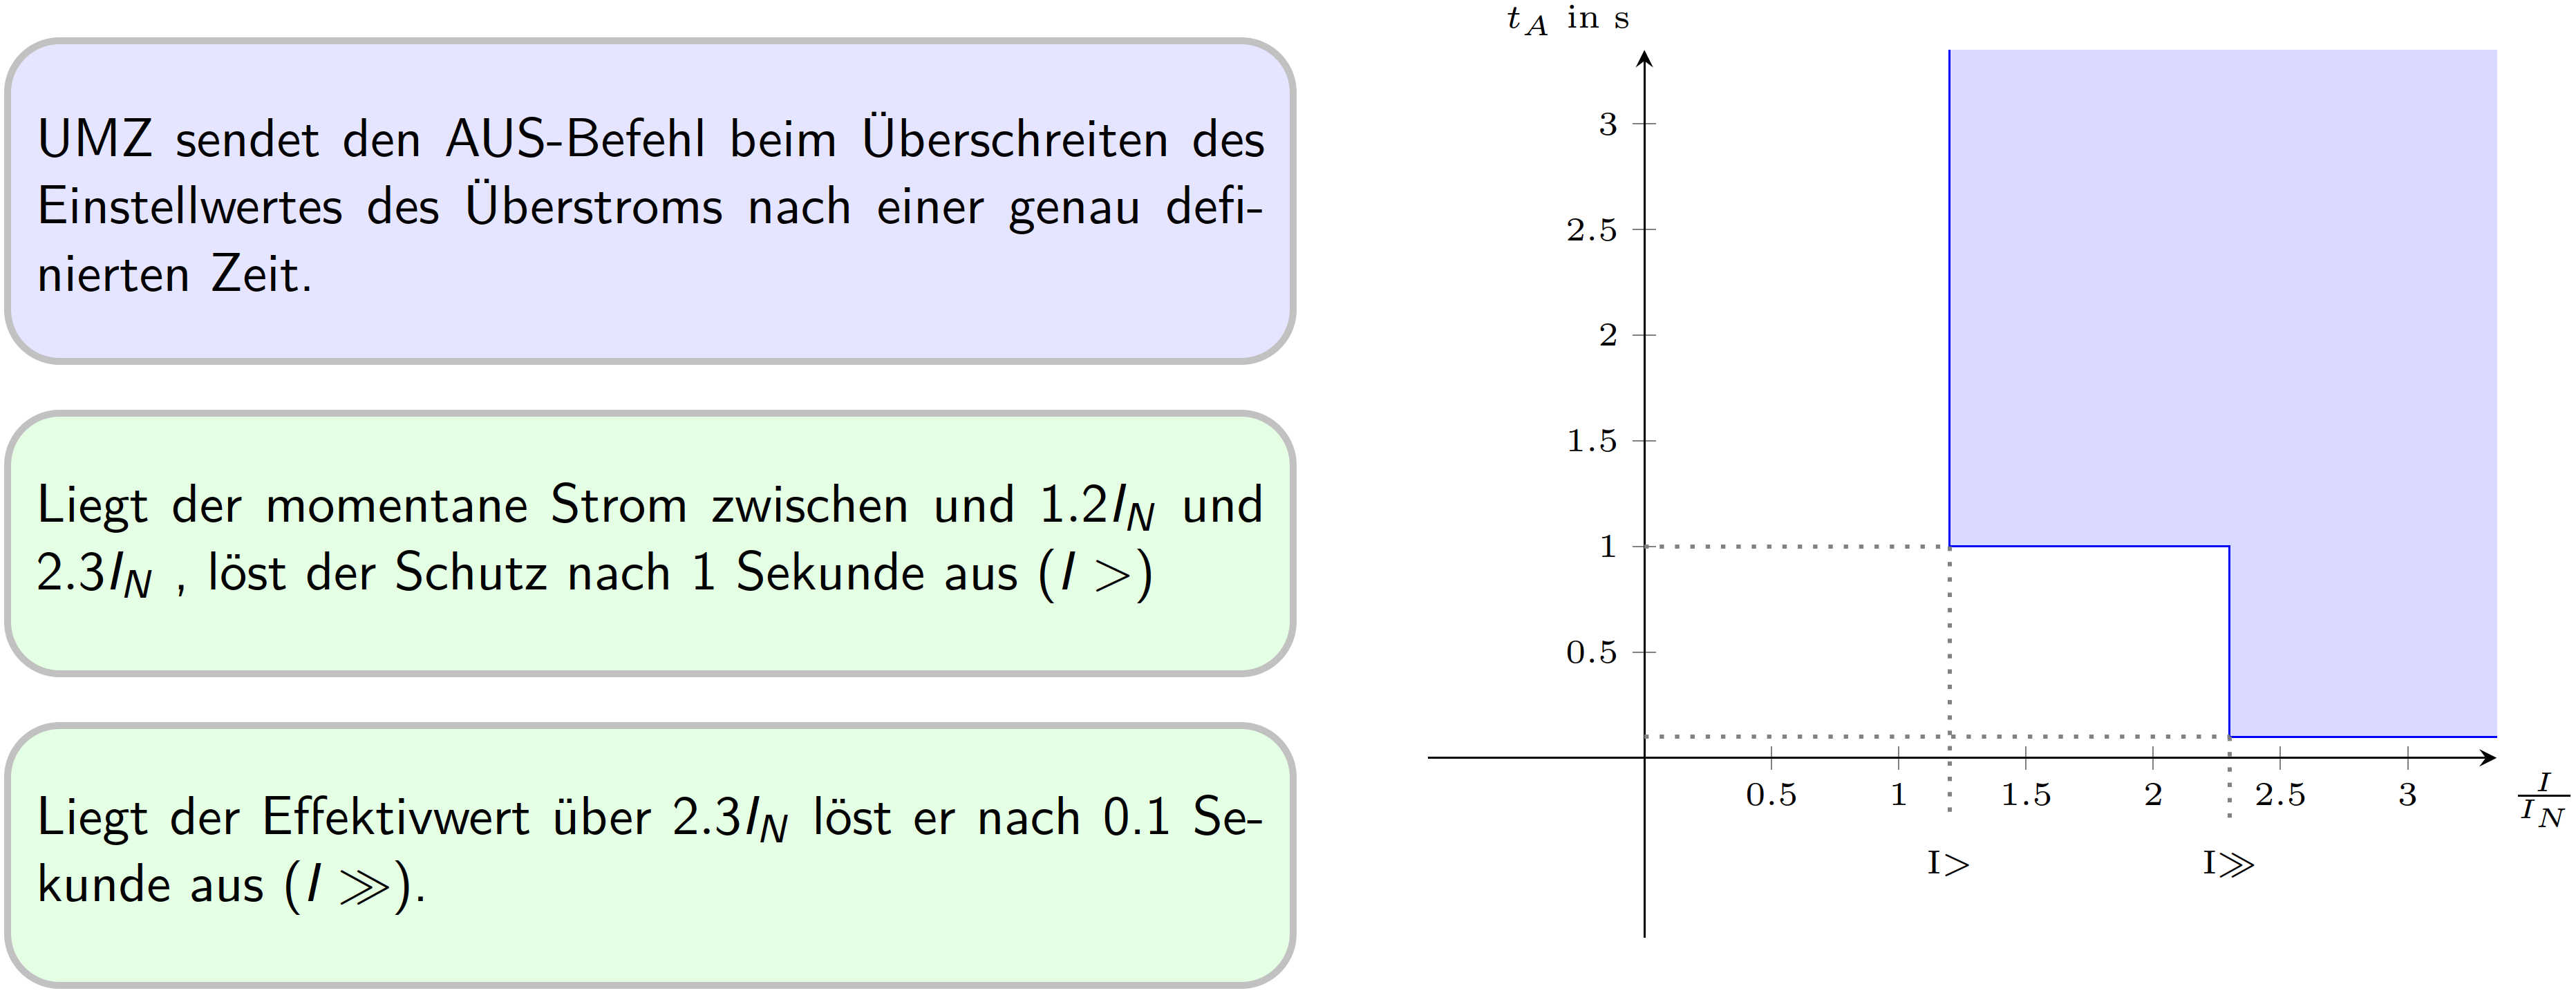
\includegraphics[width=0.8\columnwidth]{images/Schutztechnik_1.png}
    \end{center}

    \vspace{-0.2cm}

\subsection{Abhängiges Maximalstrom Zeitschutz - AMZ}
    \begin{minipage}[t]{0.35\columnwidth}
        \centering \vspace{-0.7\baselineskip}
        Als Funktion definiert

        $\boxed{t(I) = \frac{0.14}{\left( \frac{I}{I_P} \right)^{0.02} - 1} \cdot T_P}$
    \end{minipage}%
    \hfill
    \begin{minipage}[t]{0.64\columnwidth}
        \centering \vspace{-0.7\baselineskip}
        \renewcommand{\arraystretch}{1.2}
        \begin{tabular}{@{} l p{4cm} l @{}}
            $[t(I)]$      & Auslösezeit \dotfill                      & $\text{s}$ \\
            $[I]$         & Strom \dotfill                            & $\text{A}$ \\
            $[I_P]$       & Parametrierbarer Anregestrom \dotfill     & $\text{A}$ \\
            $[T_P]$       & Multiplikator \dotfill                    & $\text{s}$ \\
        \end{tabular}
    \end{minipage}

\subsection{Zeitstaffelung}
    \begin{center}
        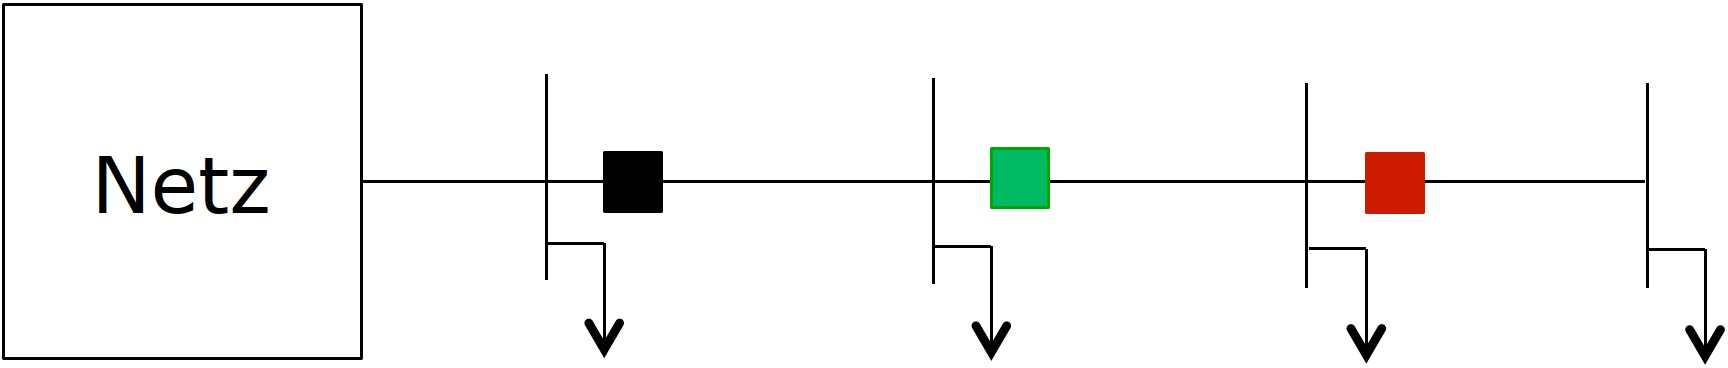
\includegraphics[width=0.8\columnwidth]{images/Schutztechnik_3.jpg}
    \end{center}

    % \vspace{0.1cm}

    \begin{minipage}[c]{0.4\columnwidth}
        \centering \vspace{-0.7\baselineskip}
        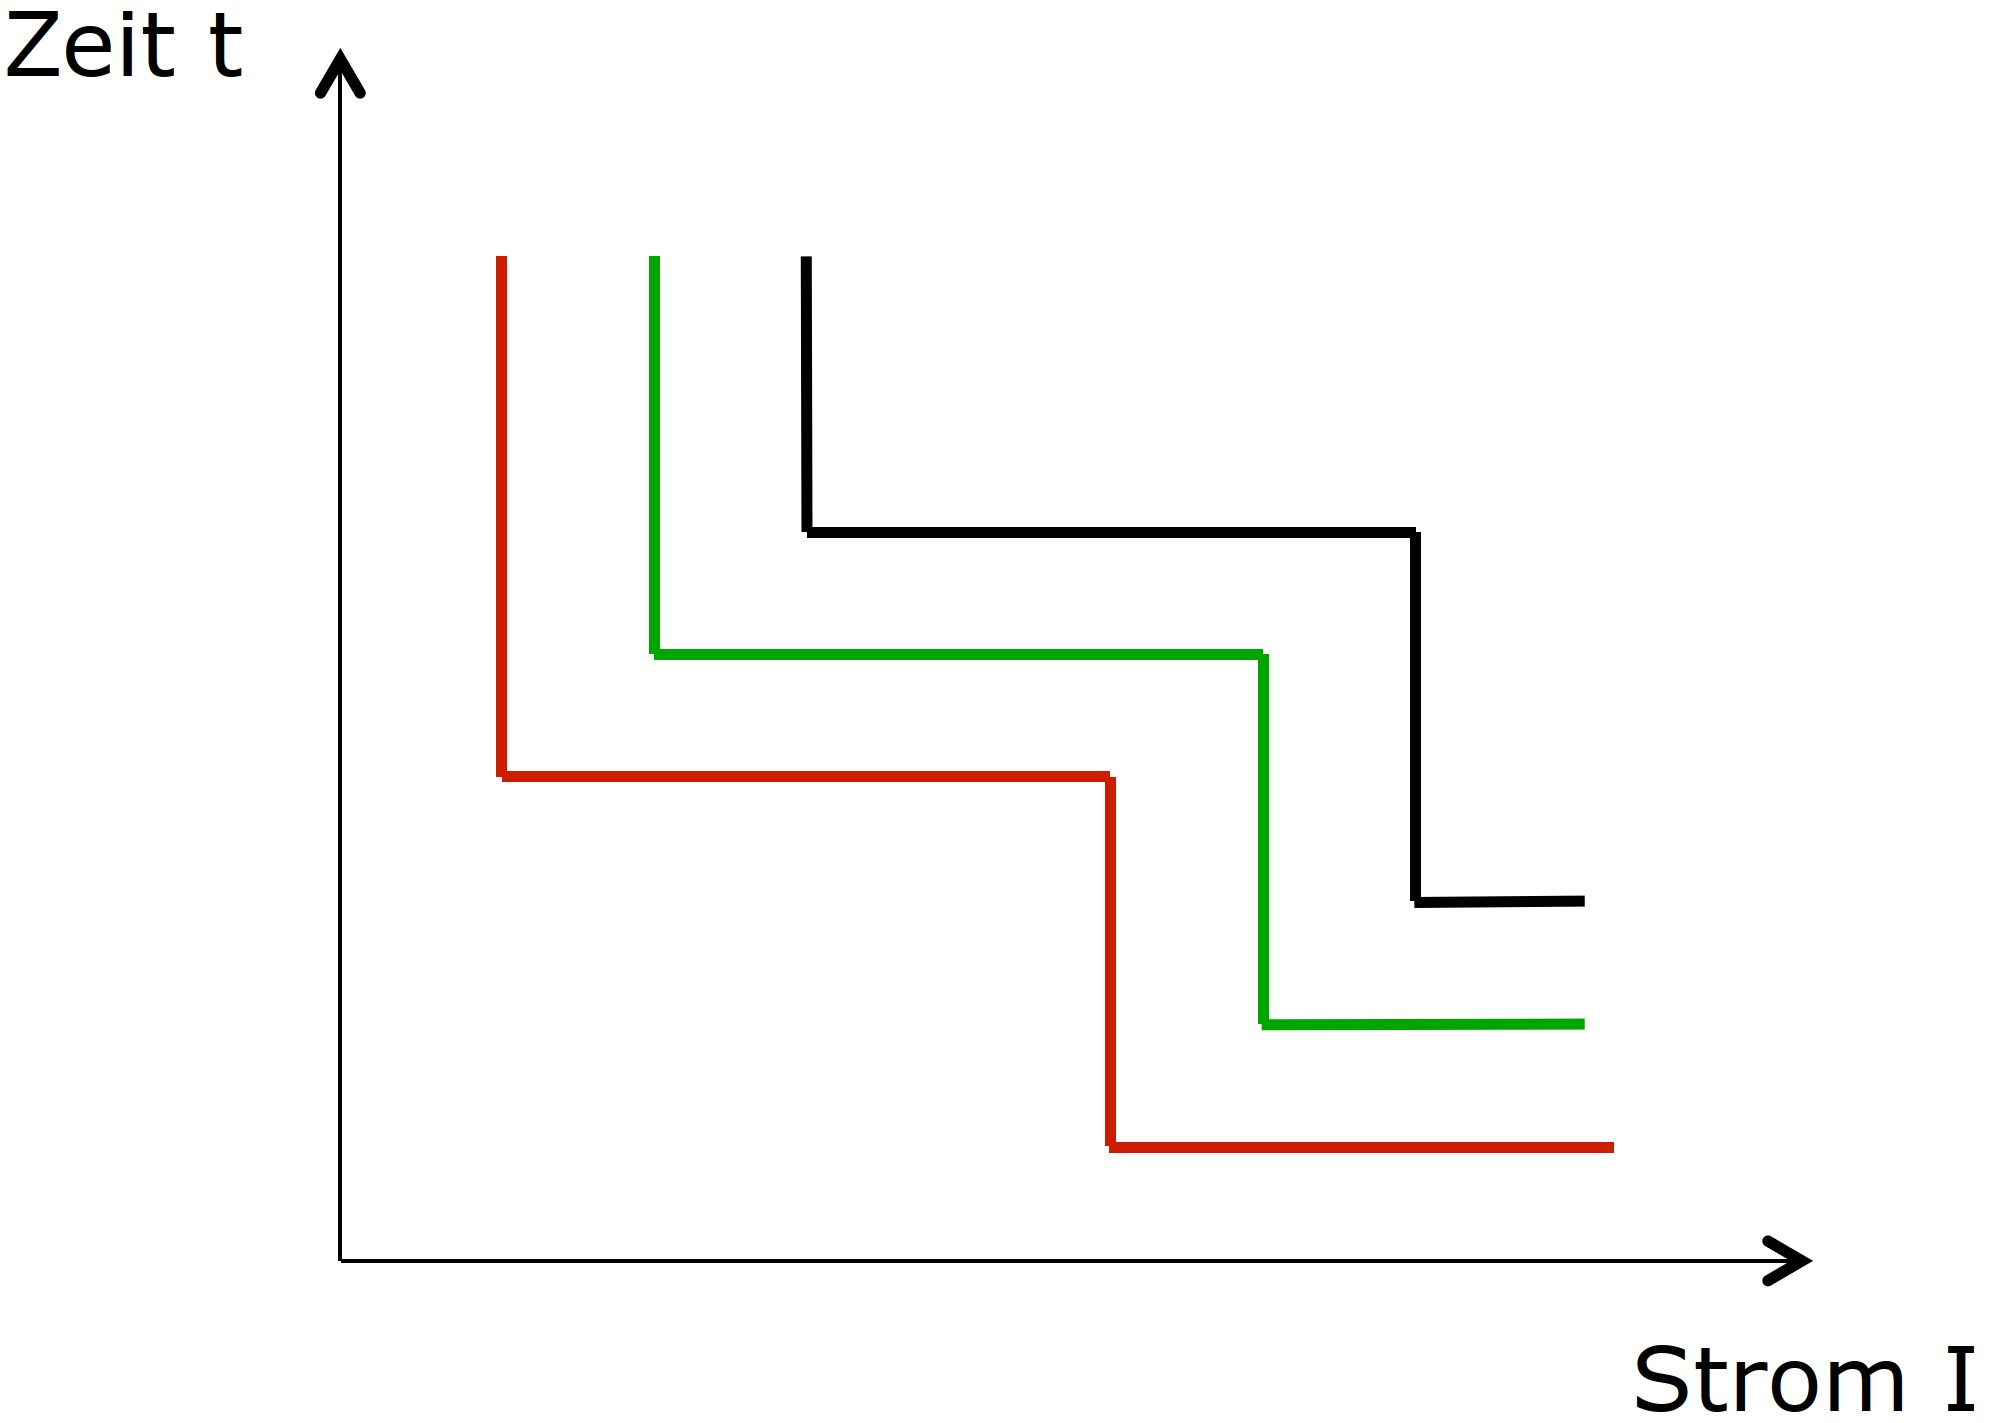
\includegraphics[width=0.9\columnwidth]{images/Schutztechnik_4.jpg}

        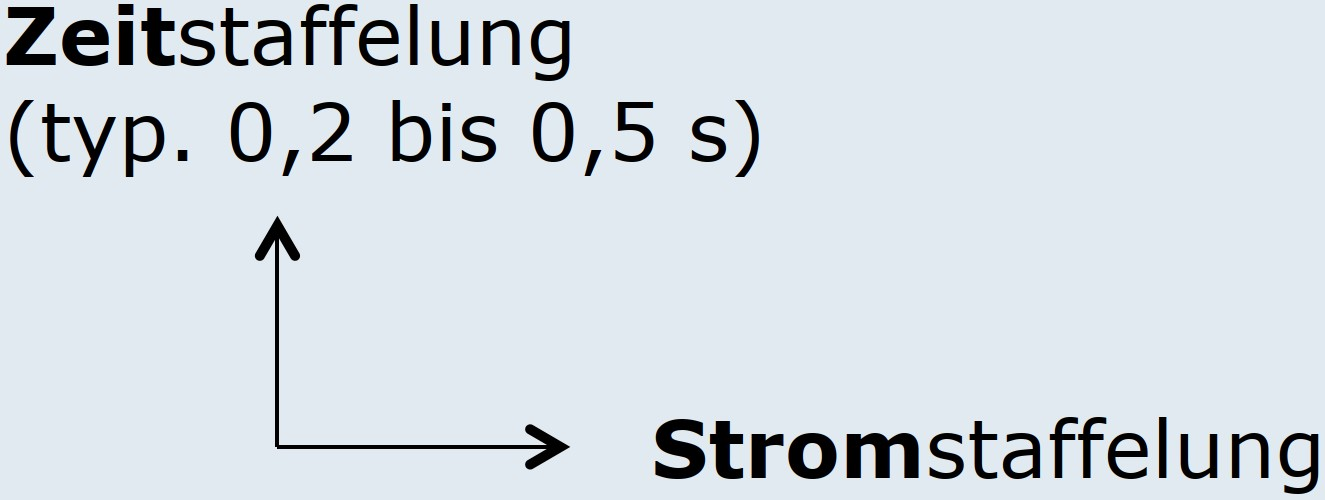
\includegraphics[width=0.8\columnwidth]{images/Schutztechnik_5.jpg} 
    \end{minipage}
    \hfill
    \begin{minipage}[c]{0.59\columnwidth}
        % \centering \vspace{-0.7\baselineskip}
        \textbf{\textcolor{green}{Vorteile:}} 
        \begin{itemize}
            \item \textbf{Einfache Methode}, den normalen Betriebszustand eines Netzes von einem Netzfehler zu unterscheiden.
        \end{itemize}
        
        % \vspace{0.1cm}
        
        \textbf{\textcolor{red}{Nachteile:}} 
        \begin{itemize}
            \item Wenn die \textbf{Einspeisung} sich \textbf{ändert}, würde der Strang unter Umständen \textit{unselektiv} abgeschaltet.
            \item In diesem Fall ist eine \textbf{Fehlerortung nicht mehr möglich}, da nur die Auslösezeit als Hilfsgrösse zur Selektion des Fehlerorts dient.
            \item Die Auslösezeit nahe der Einspeisung wird immer grösser und somit fliessen \textbf{grössere Kurzschlussströme} eine \textbf{verhältnismässig lange Zeit}.
            \item Nur in \textbf{radialen Systemen} (Strahlennetz) verwendet.
        \end{itemize}
    \end{minipage}

\subsection{Distanzschutz}
    \begin{minipage}[t]{0.42\columnwidth}
        \centering \vspace{-0.7\baselineskip}
        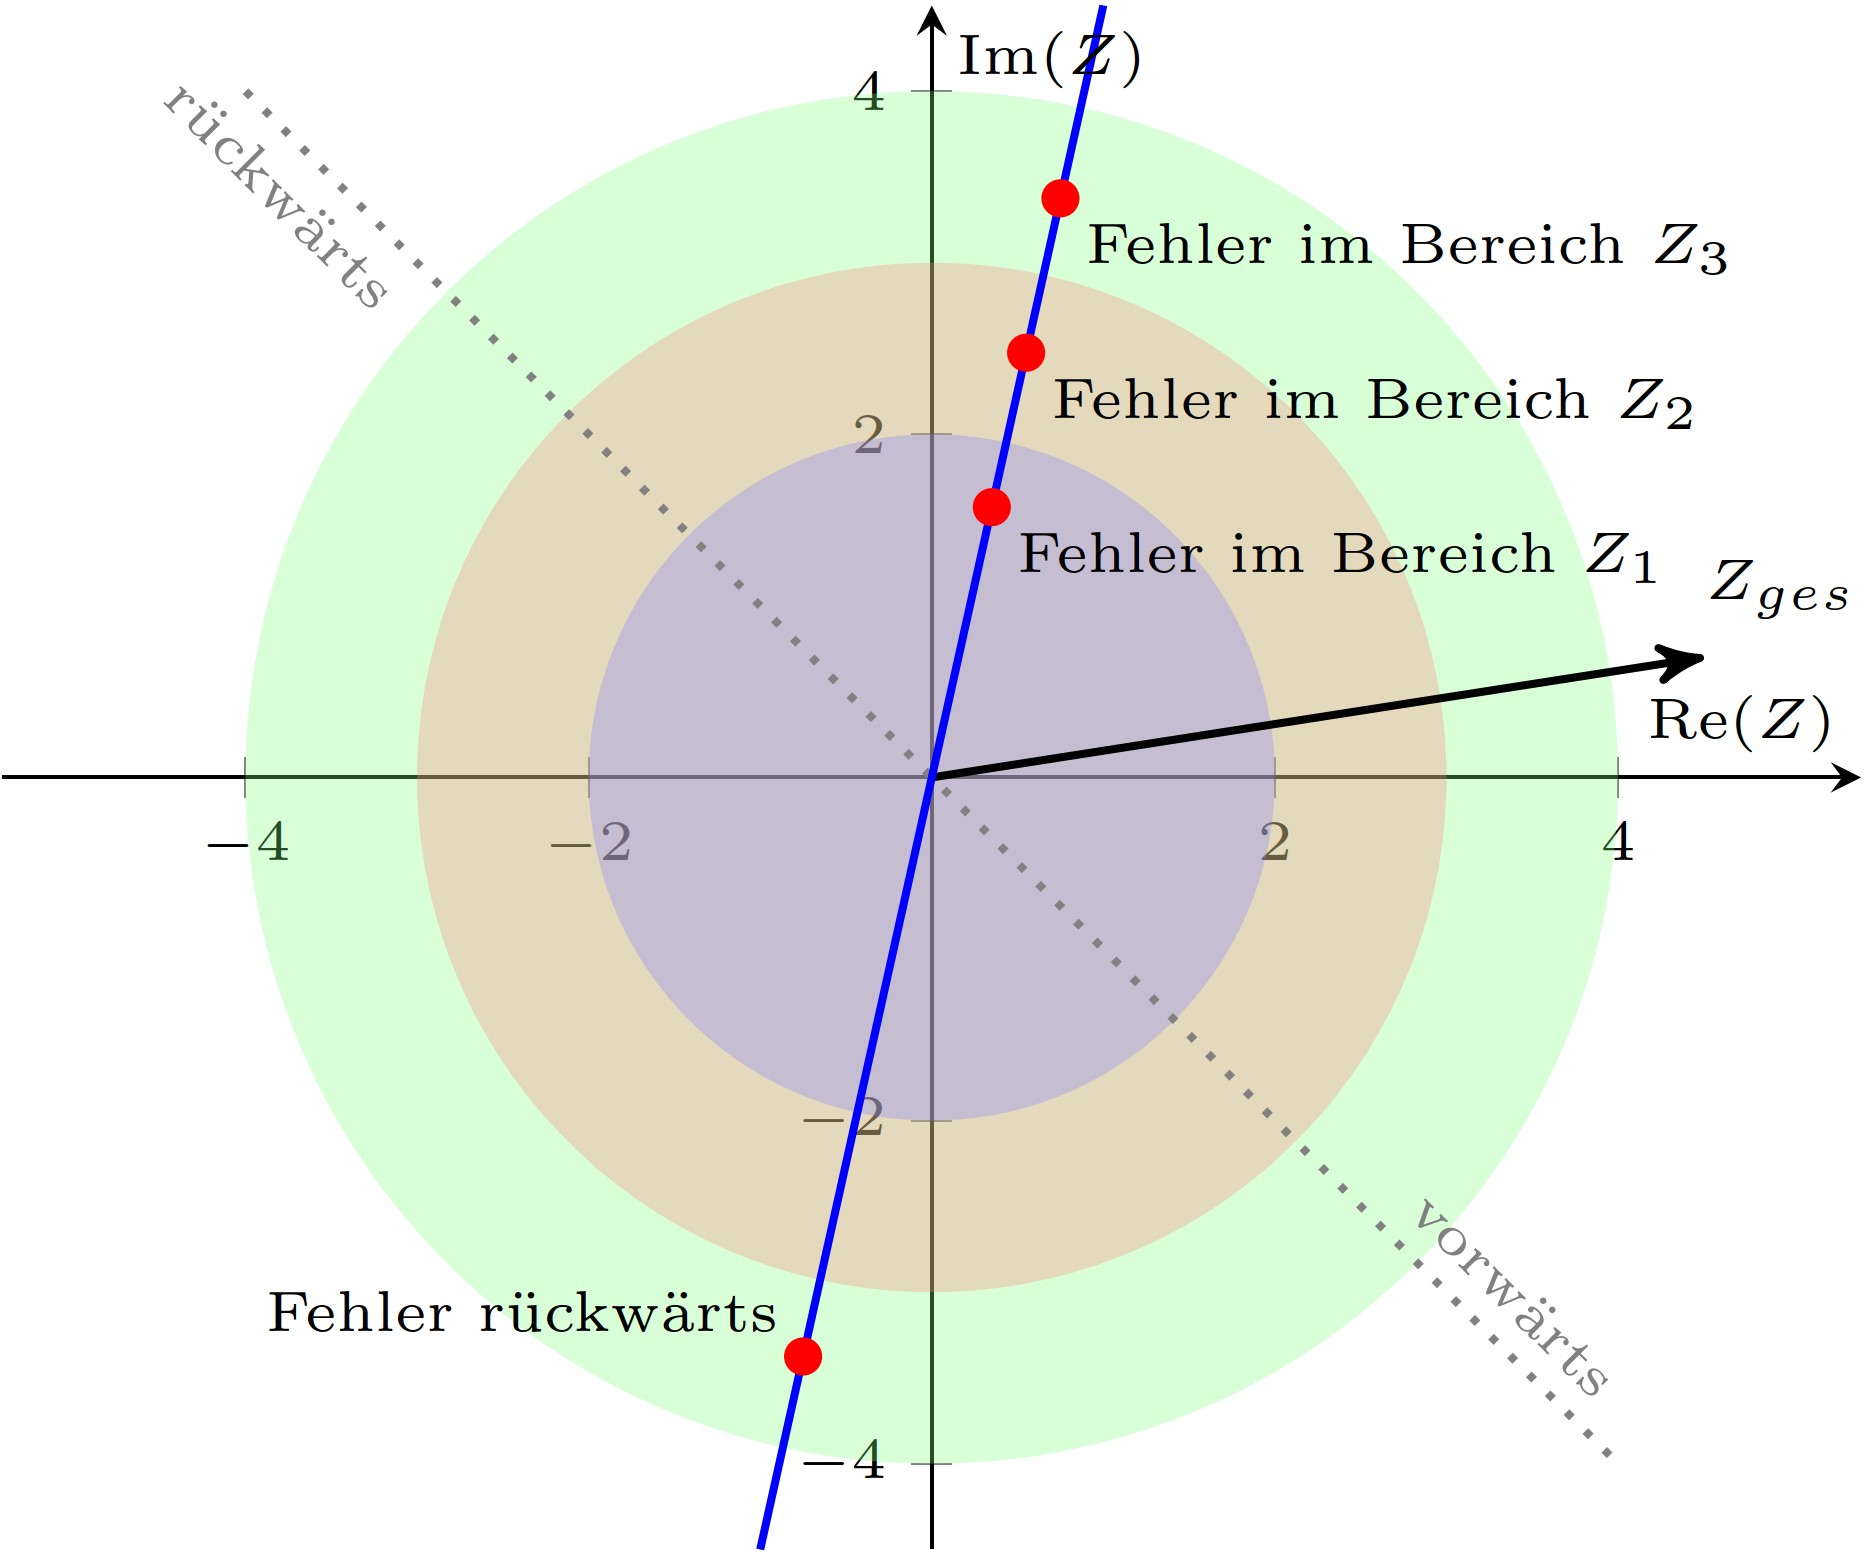
\includegraphics[width=0.95\linewidth]{images/Distanzschutz_1.jpg}
    \end{minipage}%
    \hfill
    \begin{minipage}[t]{0.57\columnwidth}
        \begin{itemize}
            \item \textbf{Nachteile des Überstromzeitschutzes}, wie etwa lange Auslösezeiten oder fehlende Selektivität bei Abweichung vom Normalschaltzustand, ist \textbf{behoben}.
            \item \textbf{Zeitstaffelschutz}, dessen Auslösezeit mit grösser werdender Entfernung zwischen Fehlerstelle und Schutzgerät-Einbauort stufig ansteigt.
            \item \textbf{Distanz \( \equiv \) Impedanz}
            \item \textbf{Reiner Kurzschlussschutz.}
            \item Aus den Messwerten der \textbf{Strom-} und \textbf{Spannungswandler} wird die \textbf{Impedanz} ermittelt.
            \item $Z_1$: Fehler nah, $Z_3$ Fehler weit weg
            \item Fehler vorwärts oder rückwärts ist aufgrund der Stromrichtung 
        \end{itemize}
    \end{minipage}

\subsubsection{Staffelplan des Distanzschutzes}
    \begin{center}
        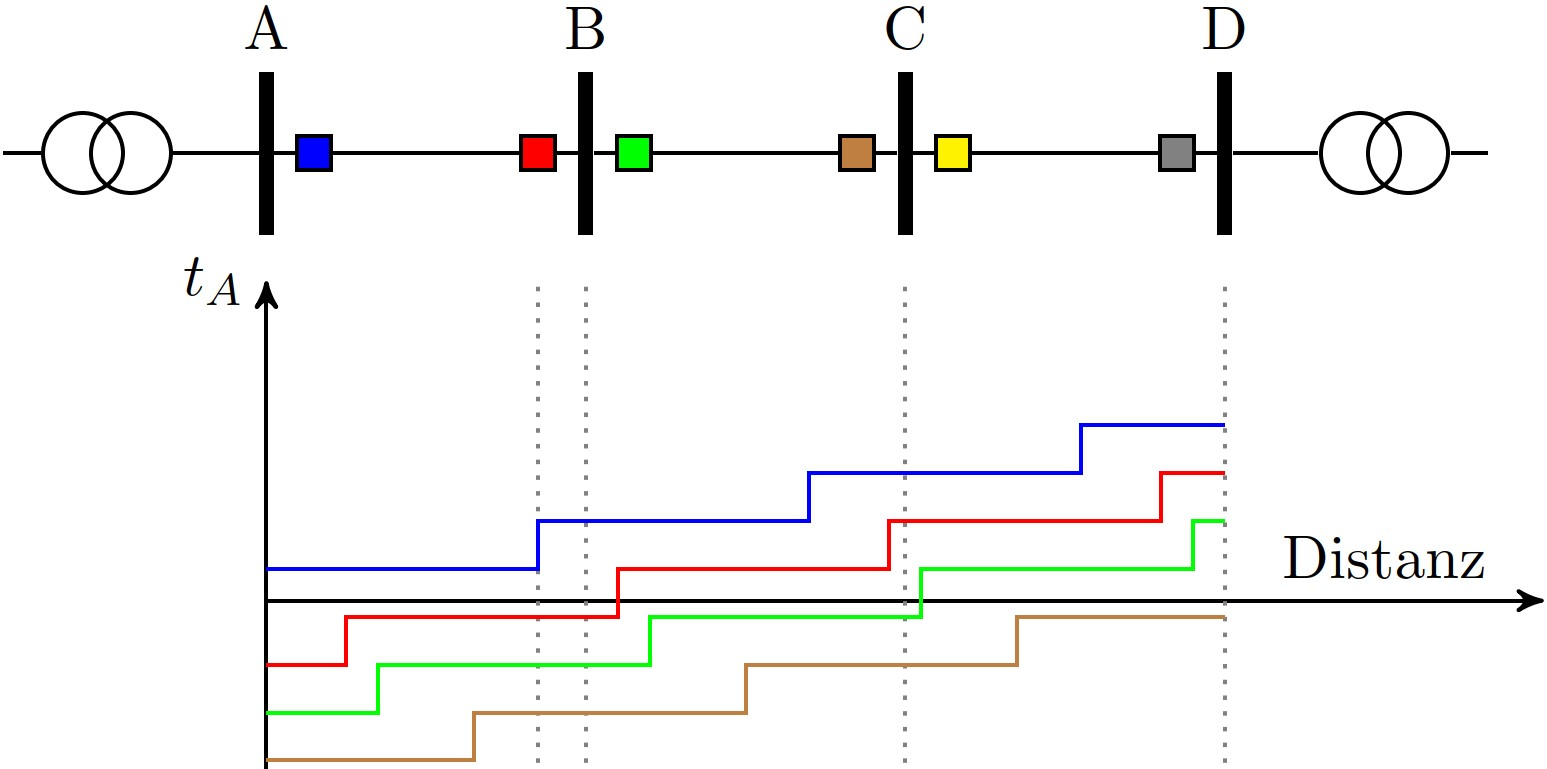
\includegraphics[width=0.8\linewidth]{images/Distanzschutz_2.jpg}
    \end{center}
    \begin{minipage}[t]{0.53\columnwidth}
        \begin{itemize}
            \item Die stufenförmige Charakteristik der Auslösekennlinien sorgt dafür, dass Netzfehler schneller abgeschaltet werden
            \item Die vorgelagerten Schutzgeräte dienen als Reserveschutz
        \end{itemize}
    \end{minipage}%
    \hfill
    \begin{minipage}[t]{0.46\columnwidth}
        \begin{itemize}
            \item Selektive Arbeitsweise des Distanzschutzes
            \item Auslösezeiten \( t_A \) in Abhängigkeit von Entfernung des Fehlers vom Relaisort
            \item Fehlerortung viel Präziser
        \end{itemize}
    \end{minipage}

\subsection{Differentialschutz}
    \begin{minipage}[t]{0.4\columnwidth}
        \centering \vspace{-0.7\baselineskip}
        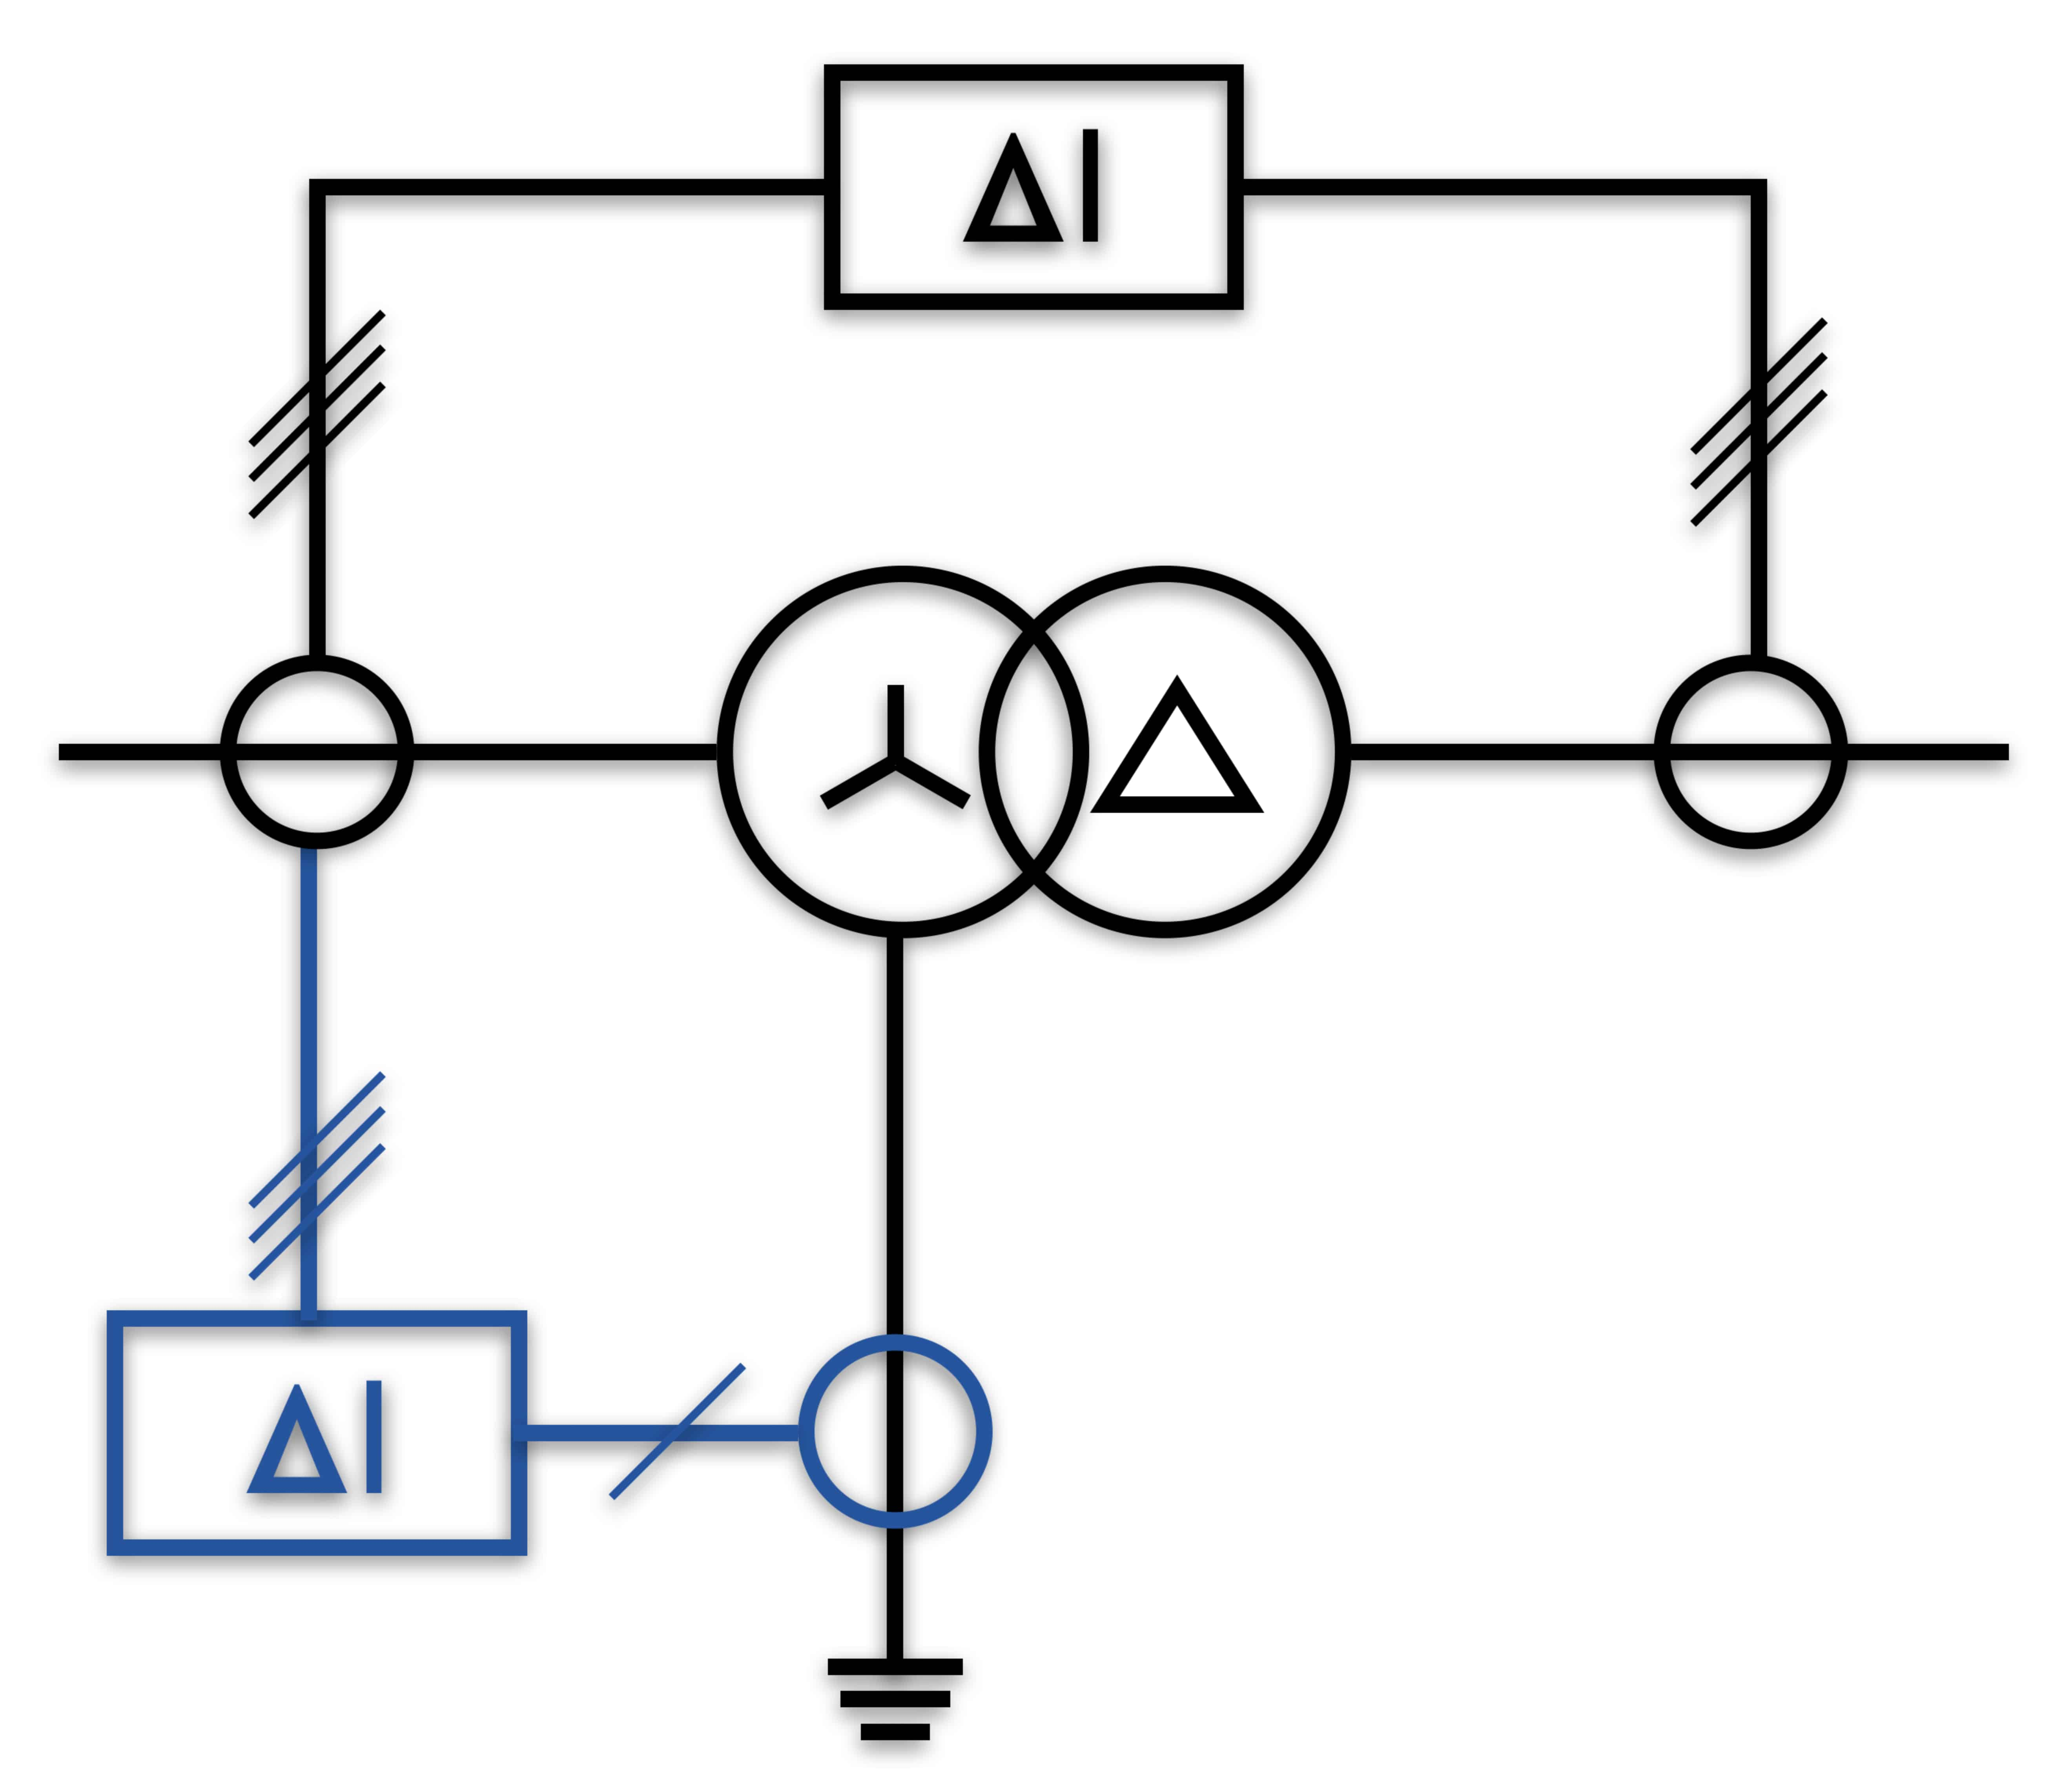
\includegraphics[width=0.95\linewidth]{images/Differentialschutz.jpg}
    \end{minipage}%
    \hfill
    \begin{minipage}[t]{0.59\columnwidth}
        \textbf{Prinzip:}
        \begin{itemize}
            \item Das Erkennungsprinzip beruht auf dem ersten kirchhoffschen Gesetz. 
            \textit{„Die Summe der zufließenden Ströme in einem elektrischen Knotenpunkt muss gleich der Summe der abfließenden Ströme sein”}
            \item \( I_{\text{Diff}} = |I_1 + I_2| > 0 \) ist Fehlerfall
            \item Wird bei Transformatoren angewendet
        \end{itemize}
    \end{minipage}

    \begin{itemize}
        \pro eine unverzögerte Abschaltung an jeder beliebigen Stelle des Schutzbereiches
        \pro Die Abgrenzung des Schutzbereichs an den Leitungsenden. Damit sind, im Gegensatz zum Distanzschutz, 100\,\% der Leitung in Schnellzeit geschützt.
        \con keine Reserveschutzfunktionen für die angrenzenden Bereiche.
    \end{itemize}

\subsection[Schwefelhexafluorid (SF6)]{Schwefelhexafluorid ($\mathrm{SF_6}$)}
    \begin{itemize} 
        \pro Sehr gute elektrische Isolierfähigkeit (hohe Durchschlagfestigkeit)
        \pro Hervorragende Lichtbogenlöscheigenschaften
        \pro Nicht brennbar, ungiftig (im reinen Zustand)
        \con Sehr hohes Treibhauspotenzial (rund 23.500x stärker als CO2)
        \con lange Lebensdauer (ca. 3.200 Jahre)
        \con Bildung giftiger Zersetzungsprodukte bei Lichtbogenentladung
    \end{itemize}
 % done
        \input{sections/70_Stabilität.tex} %done
        \input{sections/71_Frequenzregelung.tex} % done
        \section{Transiente Stabilität}
    \textit{Transiente Stabilität} bezieht sich auf die Fähigkeit der Synchronität eines zusammengeschalteten Stromnetzes, 
    nach einer Störung synchron zu bleiben. Sie hängt von der Fähigkeit ab, 
    das Gleichgewicht zwischen dem elektromagnetischen Drehmoment und dem mechanischen Drehmoment 
    jeder Synchronmaschine im System aufrechtzuerhalten bzw. wiederherzustellen.

\subsection{Mechanische zu Elektrischer Leistung}
    \begin{minipage}[t]{0.49\columnwidth}
        \centering \vspace{-0.7\baselineskip}
        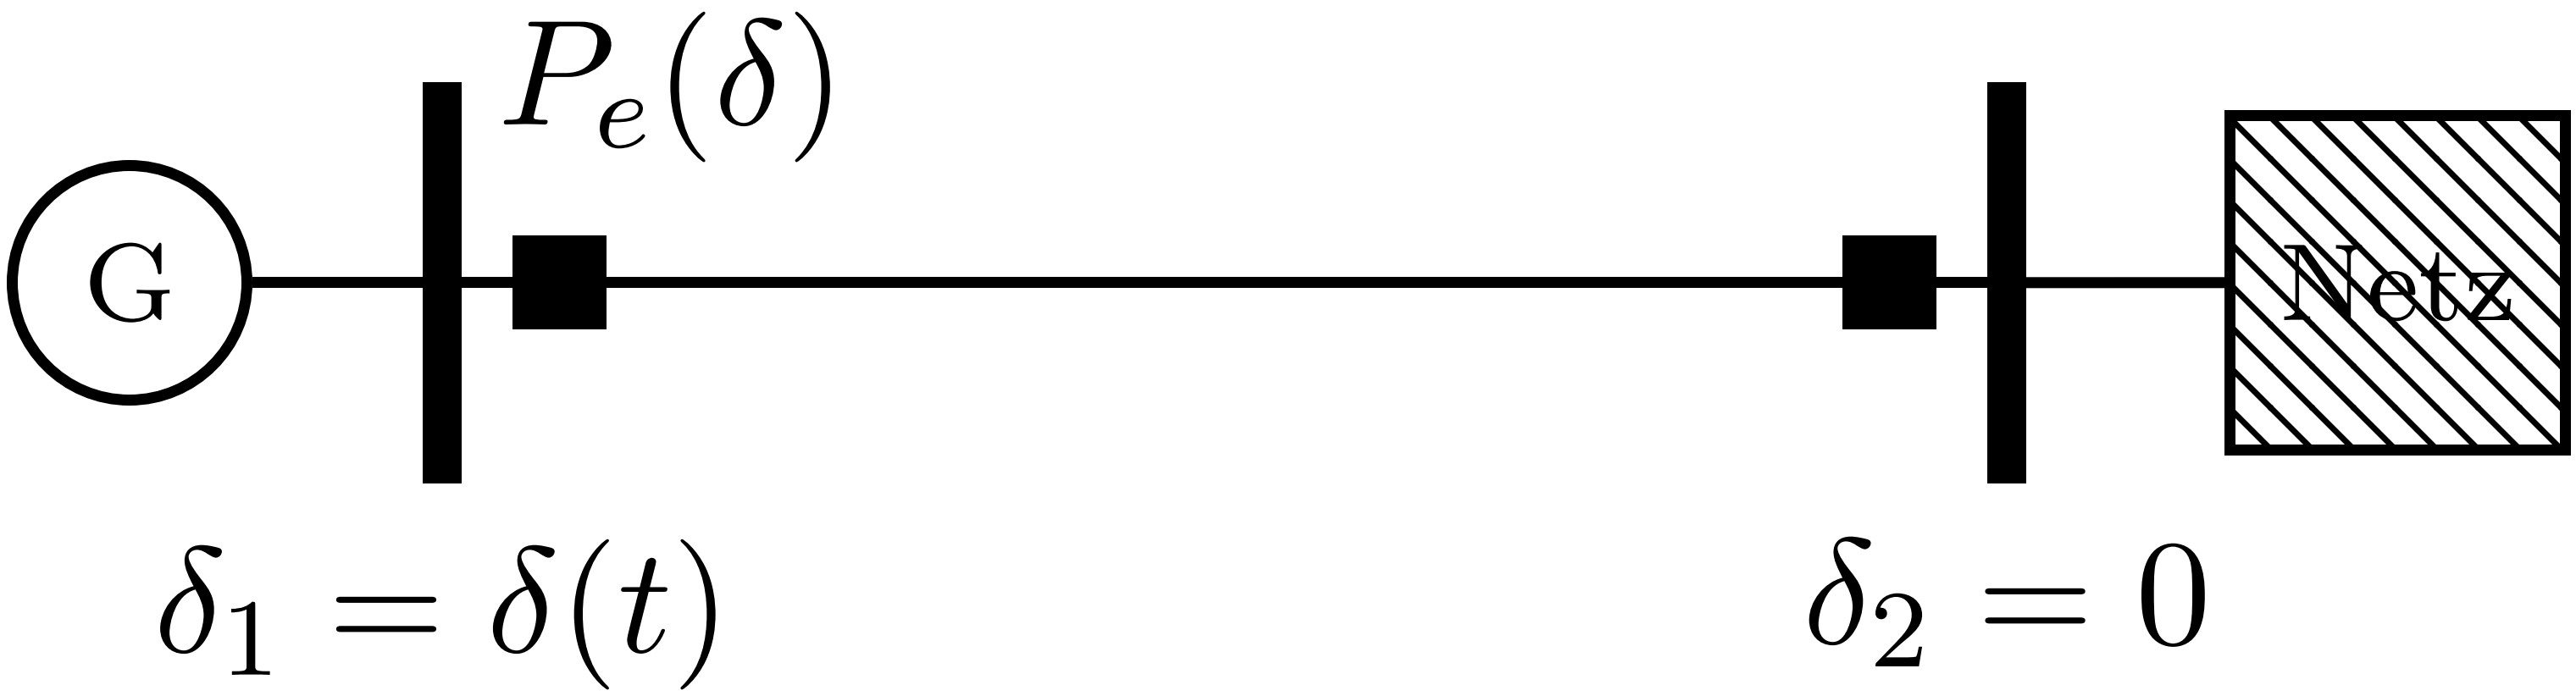
\includegraphics[width=0.95\linewidth]{images/Transiente_Stabilität.jpg}
    \end{minipage}%
    \hfill
    \begin{minipage}[t]{0.49\columnwidth}
        \centering \vspace{-0.7\baselineskip}
        $\boxed{\frac{d\omega}{dt} = \frac{P_m - P_e}{2H}}$
        $\quad$
        $\boxed{\frac{d\delta}{dt} = \omega}$
    \end{minipage}

    \vspace{0.1cm}

    Im stabilen Zustand gilt:  $P_m = P_e \; \Rightarrow \; \frac{d\omega}{dt} = 0$

\subsubsection{Fehlerfall, Lastabwurf, $P_e = 0$}
    \begin{minipage}[t]{0.49\columnwidth}
        \centering \vspace{-0.7\baselineskip}
        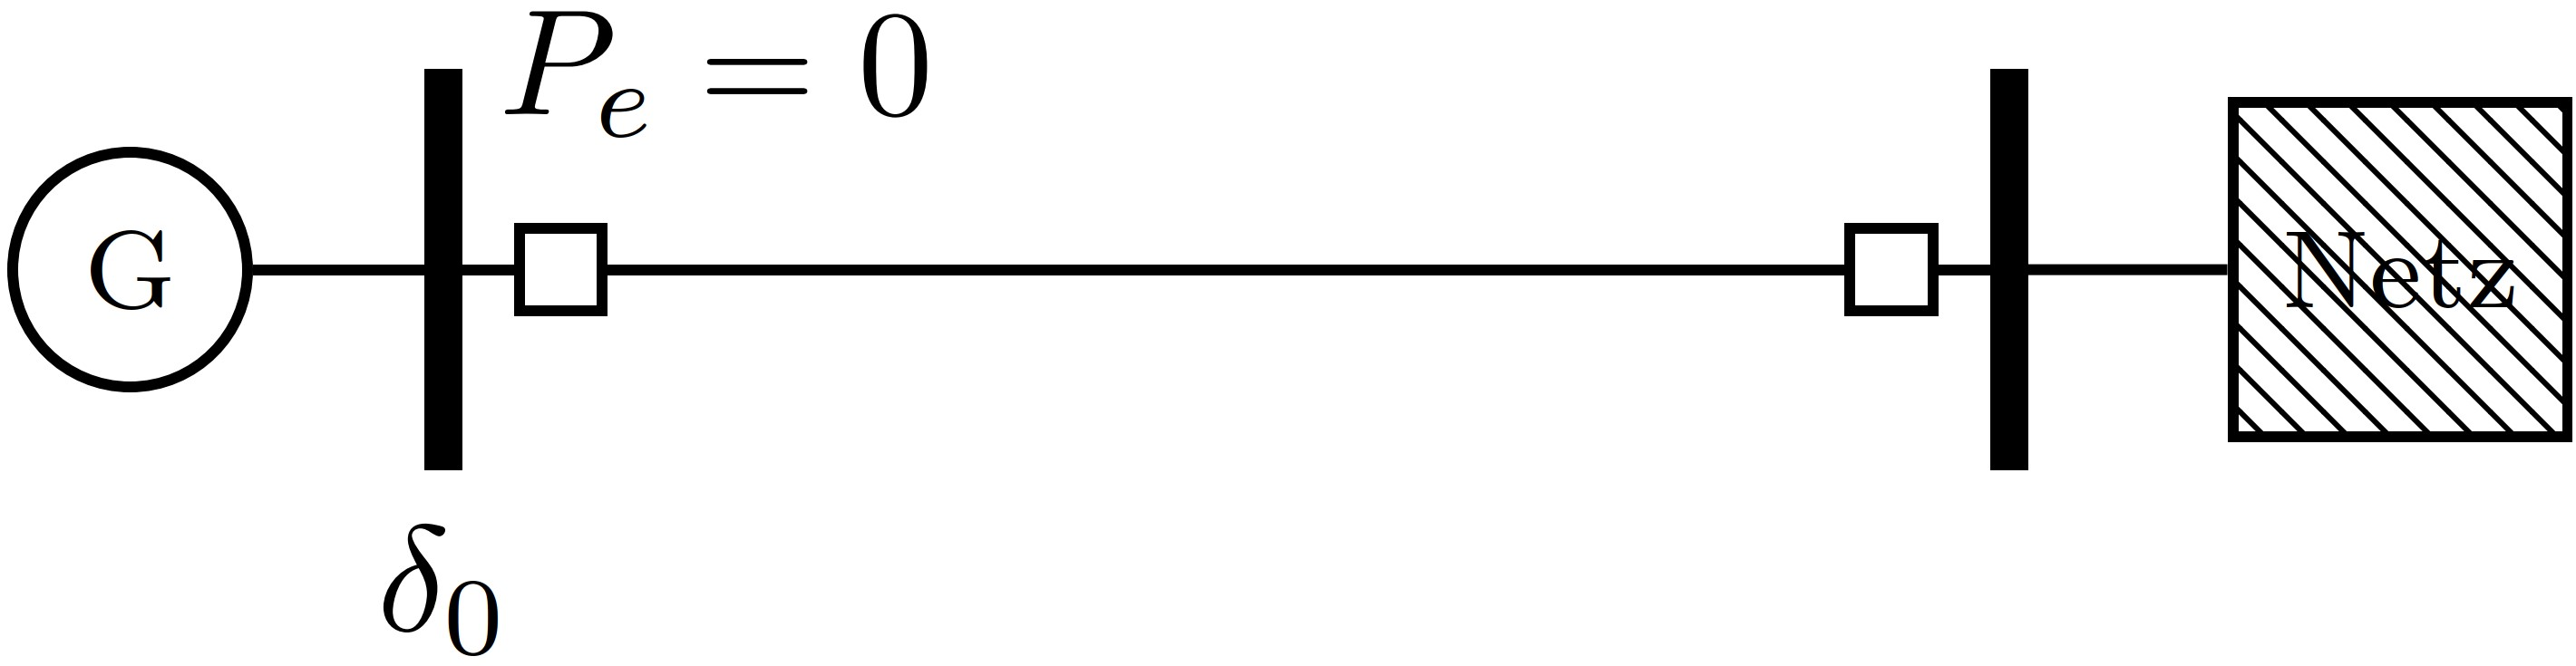
\includegraphics[width=0.95\linewidth]{images/Transiente_Stabilität_1.jpg}
    \end{minipage}%
    \hfill
    \begin{minipage}[t]{0.49\columnwidth}
        \centering \vspace{-0.7\baselineskip}
        $\boxed{\frac{d\omega}{dt} = \frac{P_m - P_{e}\big|_{=0}}{2H}}$
        $\quad$
        $\boxed{\frac{d\delta}{dt} = \omega}$
    \end{minipage}

    \vspace{0.1cm}

    \begin{minipage}[t]{0.35\columnwidth}
        \vspace{-0.3\baselineskip}
        Der Generator muss die von der Turbine zugeführte Energie $P_m$ aufnehmen, indem er seine kinetische Energie erhöht, d.h. beschleunigt:
        
        \vspace{0.1cm}
        
        $\frac{d\omega}{dt} > 0,\quad \omega \uparrow,\quad \delta \uparrow$
    \end{minipage}%
    \hfill
    \begin{minipage}[t]{0.59\columnwidth}
        \centering \vspace{-0.7\baselineskip}
        \renewcommand{\arraystretch}{1.2}
        \begin{tabular}{@{} l p{4cm} l @{}}
            $[\omega]$     & Winkelgeschwindigkeit \dotfill              & $\frac{\text{rad}}{\text{s}}$ \\
            $[t]$          & Zeit \dotfill                               & $\text{s}$ \\
            $[P_m]$        & mechanische Leistung \dotfill               & $\text{W}$ \\
            $[P_e]$        & elektrische Leistung \dotfill               & $\text{W}$ \\
            $[H]$          & Trägheitsfaktor \dotfill & - \\
            $[\delta]$     & Polradwinkel \dotfill                        & $\text{rad}$ \\
        \end{tabular}
    \end{minipage}

\subsubsection{Wiedereinschalten nach Fehlerfall}
    \begin{minipage}[t]{0.49\columnwidth}
        \centering \vspace{-0.7\baselineskip}
        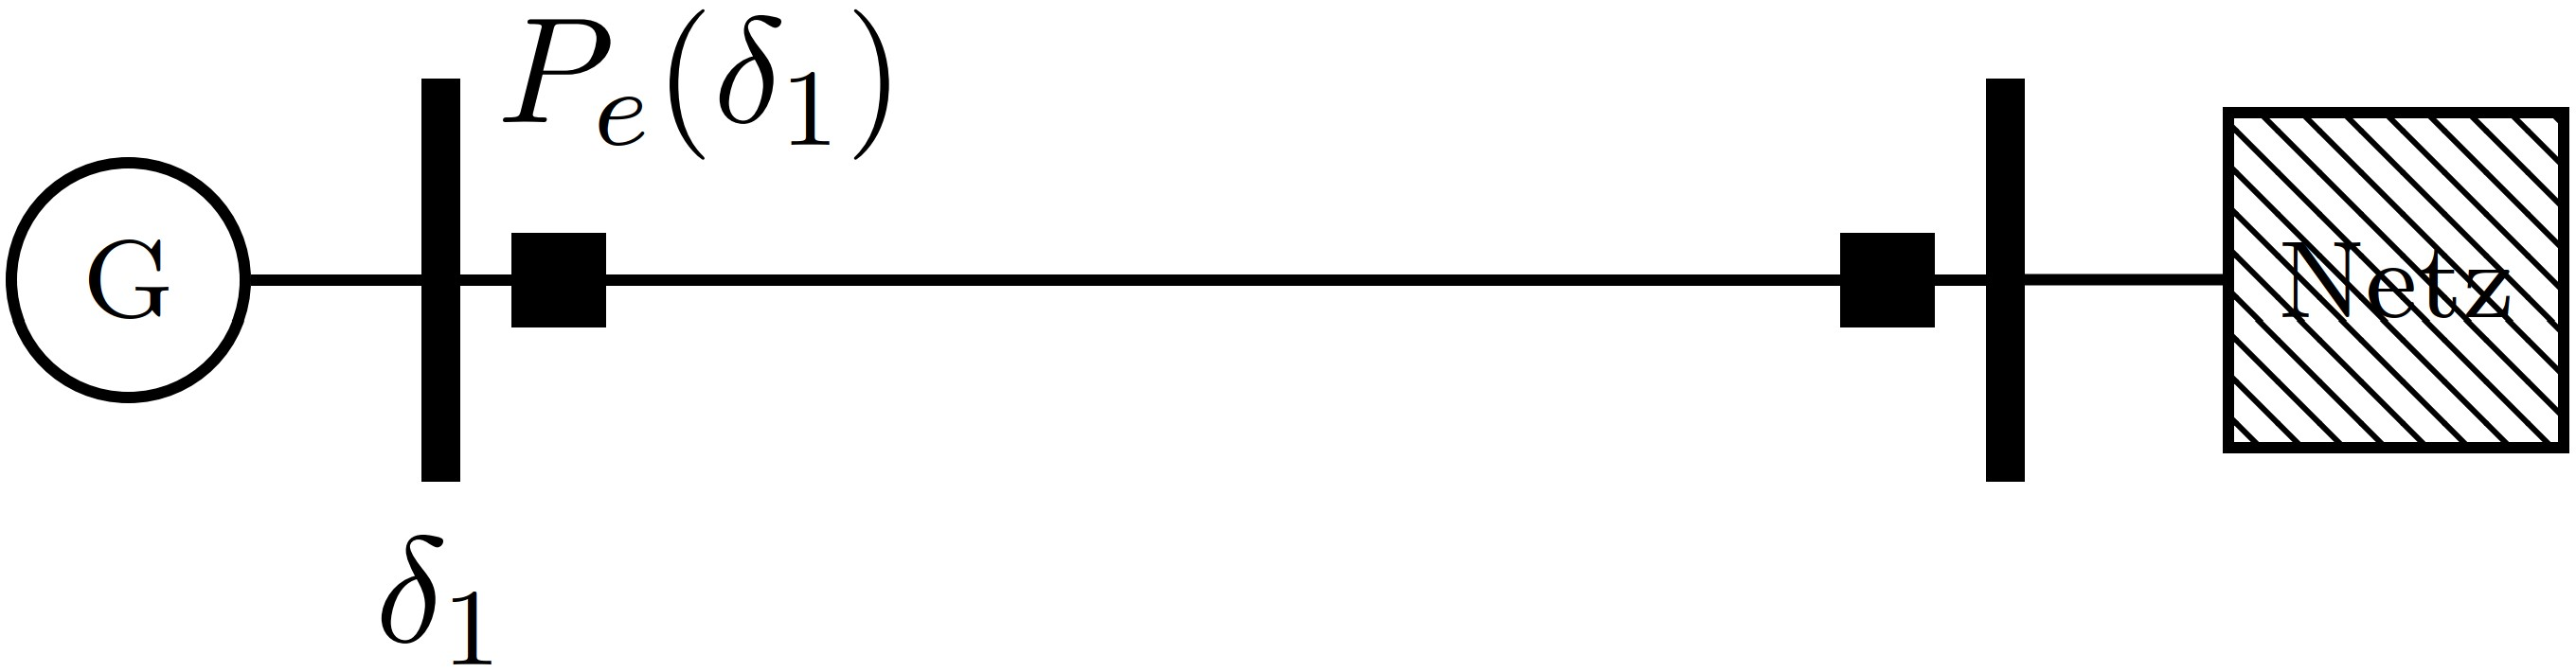
\includegraphics[width=0.95\linewidth]{images/Transiente_Stabilität_2.jpg}
    \end{minipage}%
    \hfill
    \begin{minipage}[t]{0.49\columnwidth}
        Nach wenigen Sekundenbruchteilen kommt es zu einer sogenannten automatischen Wiedereinschaltung: 
        In der Hoffnung, dass der Lichtbogen erloschen ist, schaltet das Schutzgerät die Leitung wieder zu. 
        
    \end{minipage}

    Die Schalter an beiden Leitungsenden werden nach Ablauf der Wiedereinschaltzeit (z.\,B. 500 ms) geschlossen.

    \vspace{0.1cm}

    In dieser Zeit ist $\delta$ gestiegen ($\delta = \delta_1$). Bei der Wiedereinschaltung ist $P_e(\delta_1) > P_m$. 

    Der Generator bremst und baut so die überschüssige kinetische Energie ab.

\subsection{Flächenkriterium}
\begin{minipage}[t]{0.45\columnwidth}
    \centering \vspace{-0.7\baselineskip}
    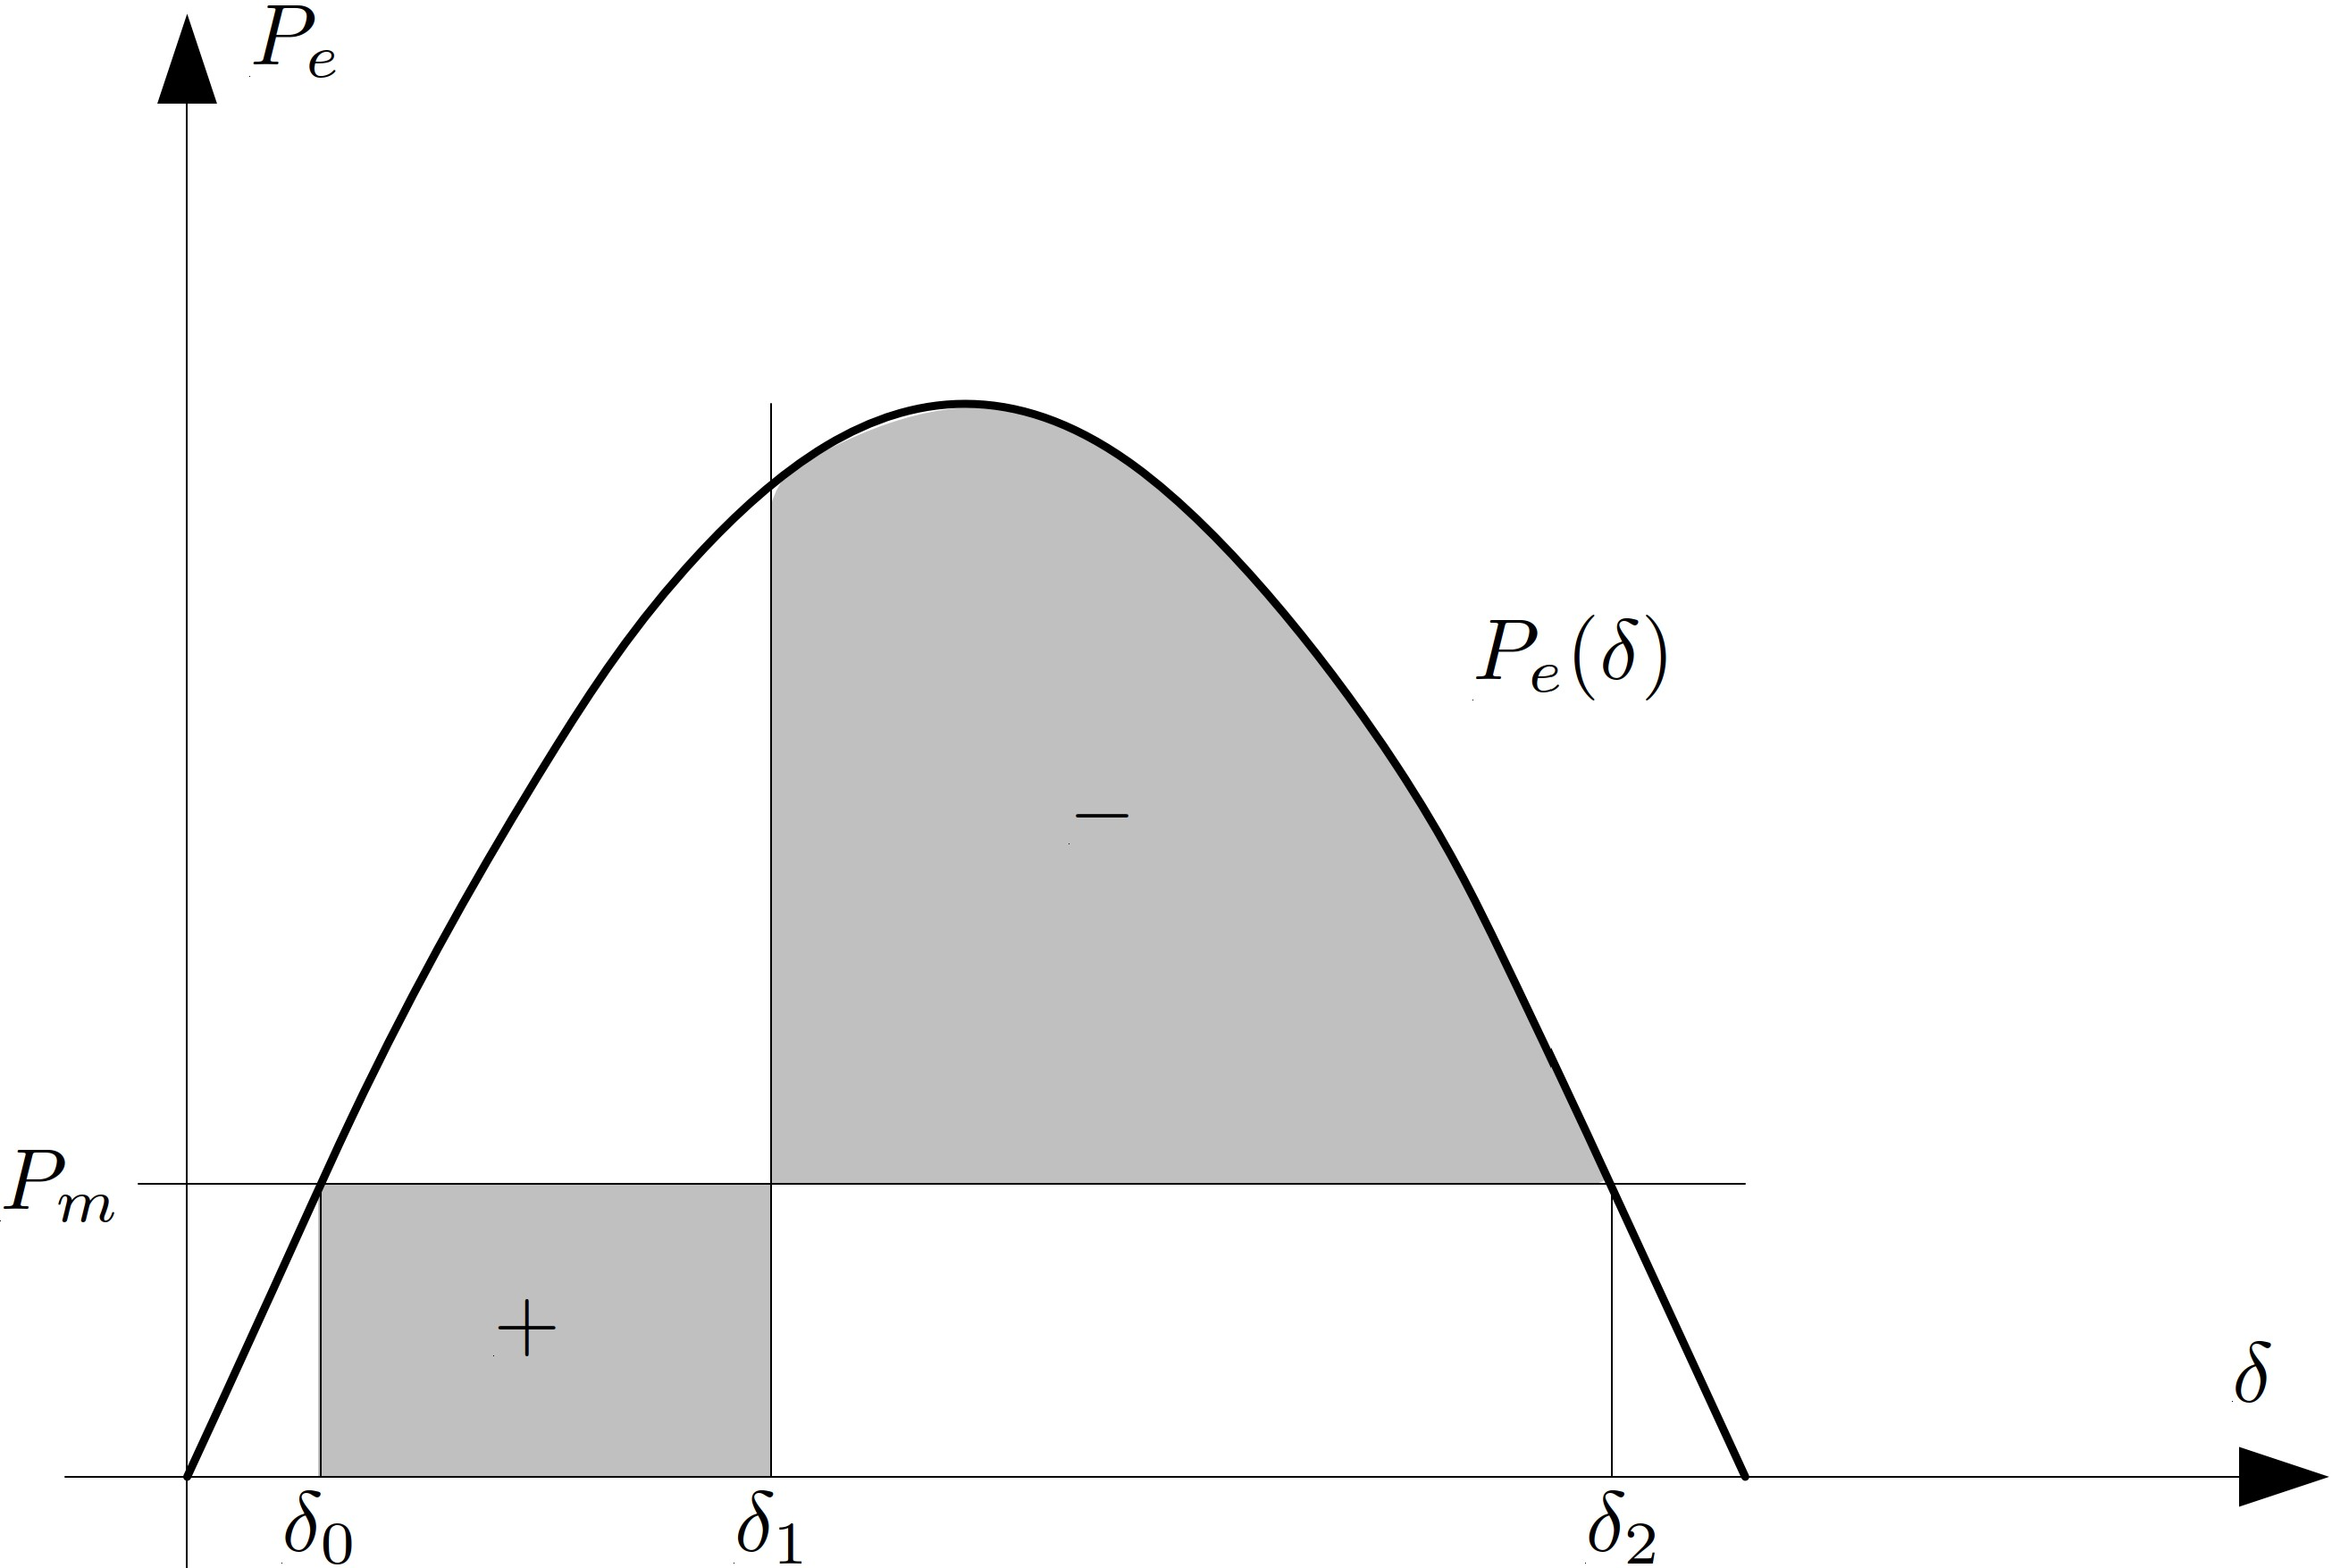
\includegraphics[width=0.85\linewidth]{images/Transiente_Stabilität_3.jpg}
\end{minipage}%
\hfill
\begin{minipage}[t]{0.54\columnwidth}
    \begin{itemize}
        \pro Fläche entspricht der Energie, die der Generator währen einer halben Sekunde aufnehmen muss
        \con Fläche entspricht der maximalen Energie, welche der Generator wieder abbauen kann
        \item Flächenkriterium: - Fläche muss grösser sein als + Fläche
        \item[]$\Rightarrow $\textbf{Flächenbeseitigungszeit} enorm wichtig
    \end{itemize}
\end{minipage} % done
        \section{Spannungsregelung}
    Unter Spannungsstabilität versteht man die Fähigkeit eines Stromversorgungssystems, 
    an allen Bussen (Knoten) im System konstante Spannungen aufrechtzuerhalten, 
    nachdem es einer Störung aus einem gegebenen Betriebszustand ausgesetzt wurde.

\subsection{Spannungskollaps}
    \begin{itemize}
        \item Spannung zu hoch: Isolationsdurchbruch
        \item Spannung zu tief: Spannungskollaps
        \item Abhängig von Nasenkurve
    \end{itemize}

    \vspace{-0.3cm}

    \begin{center}
        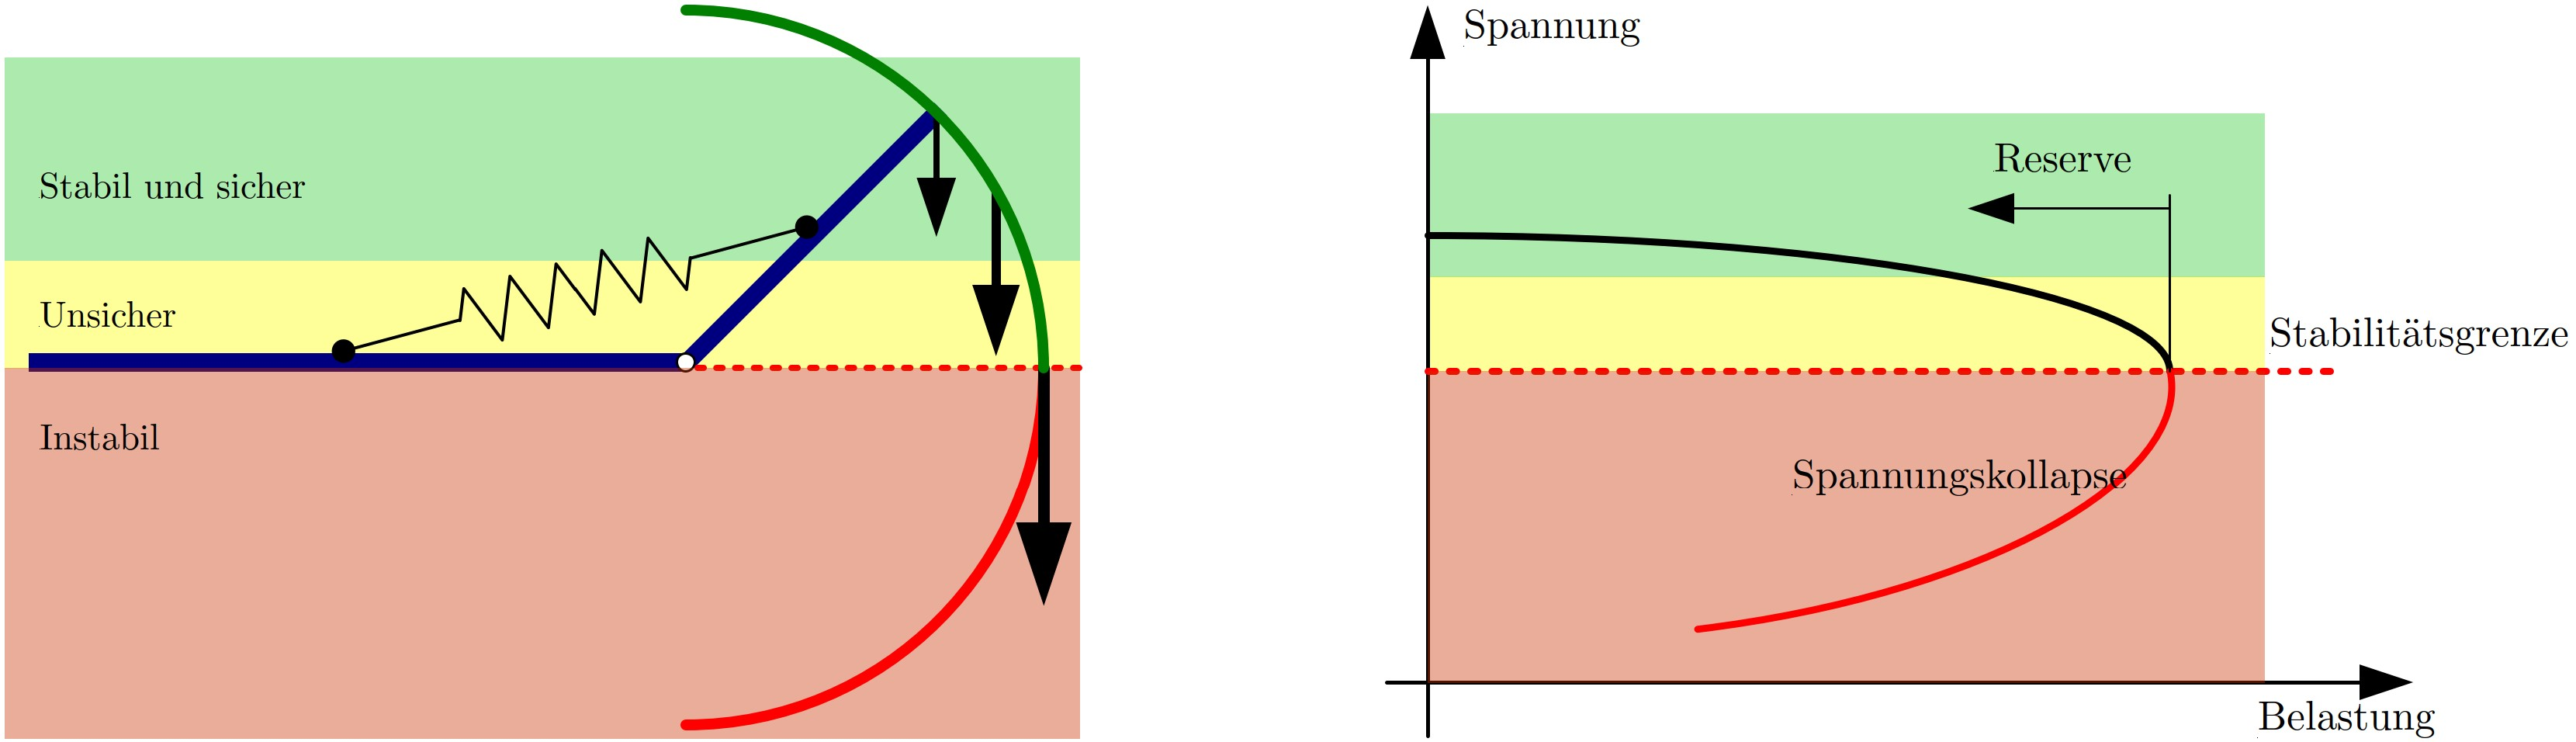
\includegraphics[width=0.9\columnwidth]{images/Spannungsregelung_1.jpg}
    \end{center}

    \vspace{-0.4cm}

    \begin{center}
        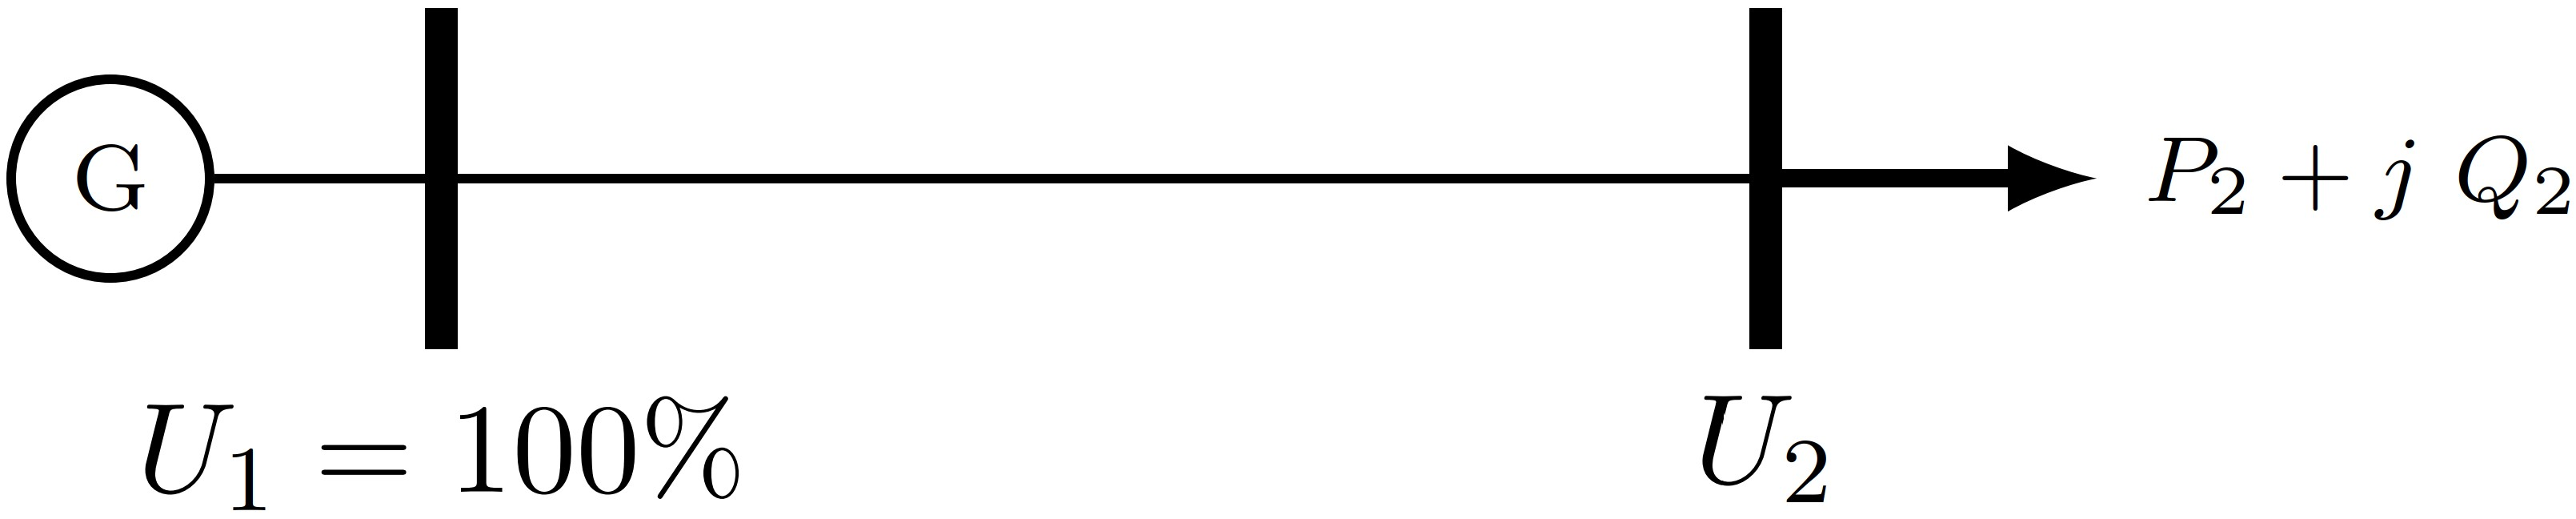
\includegraphics[width=0.45\columnwidth]{images/Spannungsregelung_2.jpg}
    \end{center}

    \vspace{-0.3cm}

    \begin{minipage}[c]{0.48\columnwidth}
        \begin{center}
            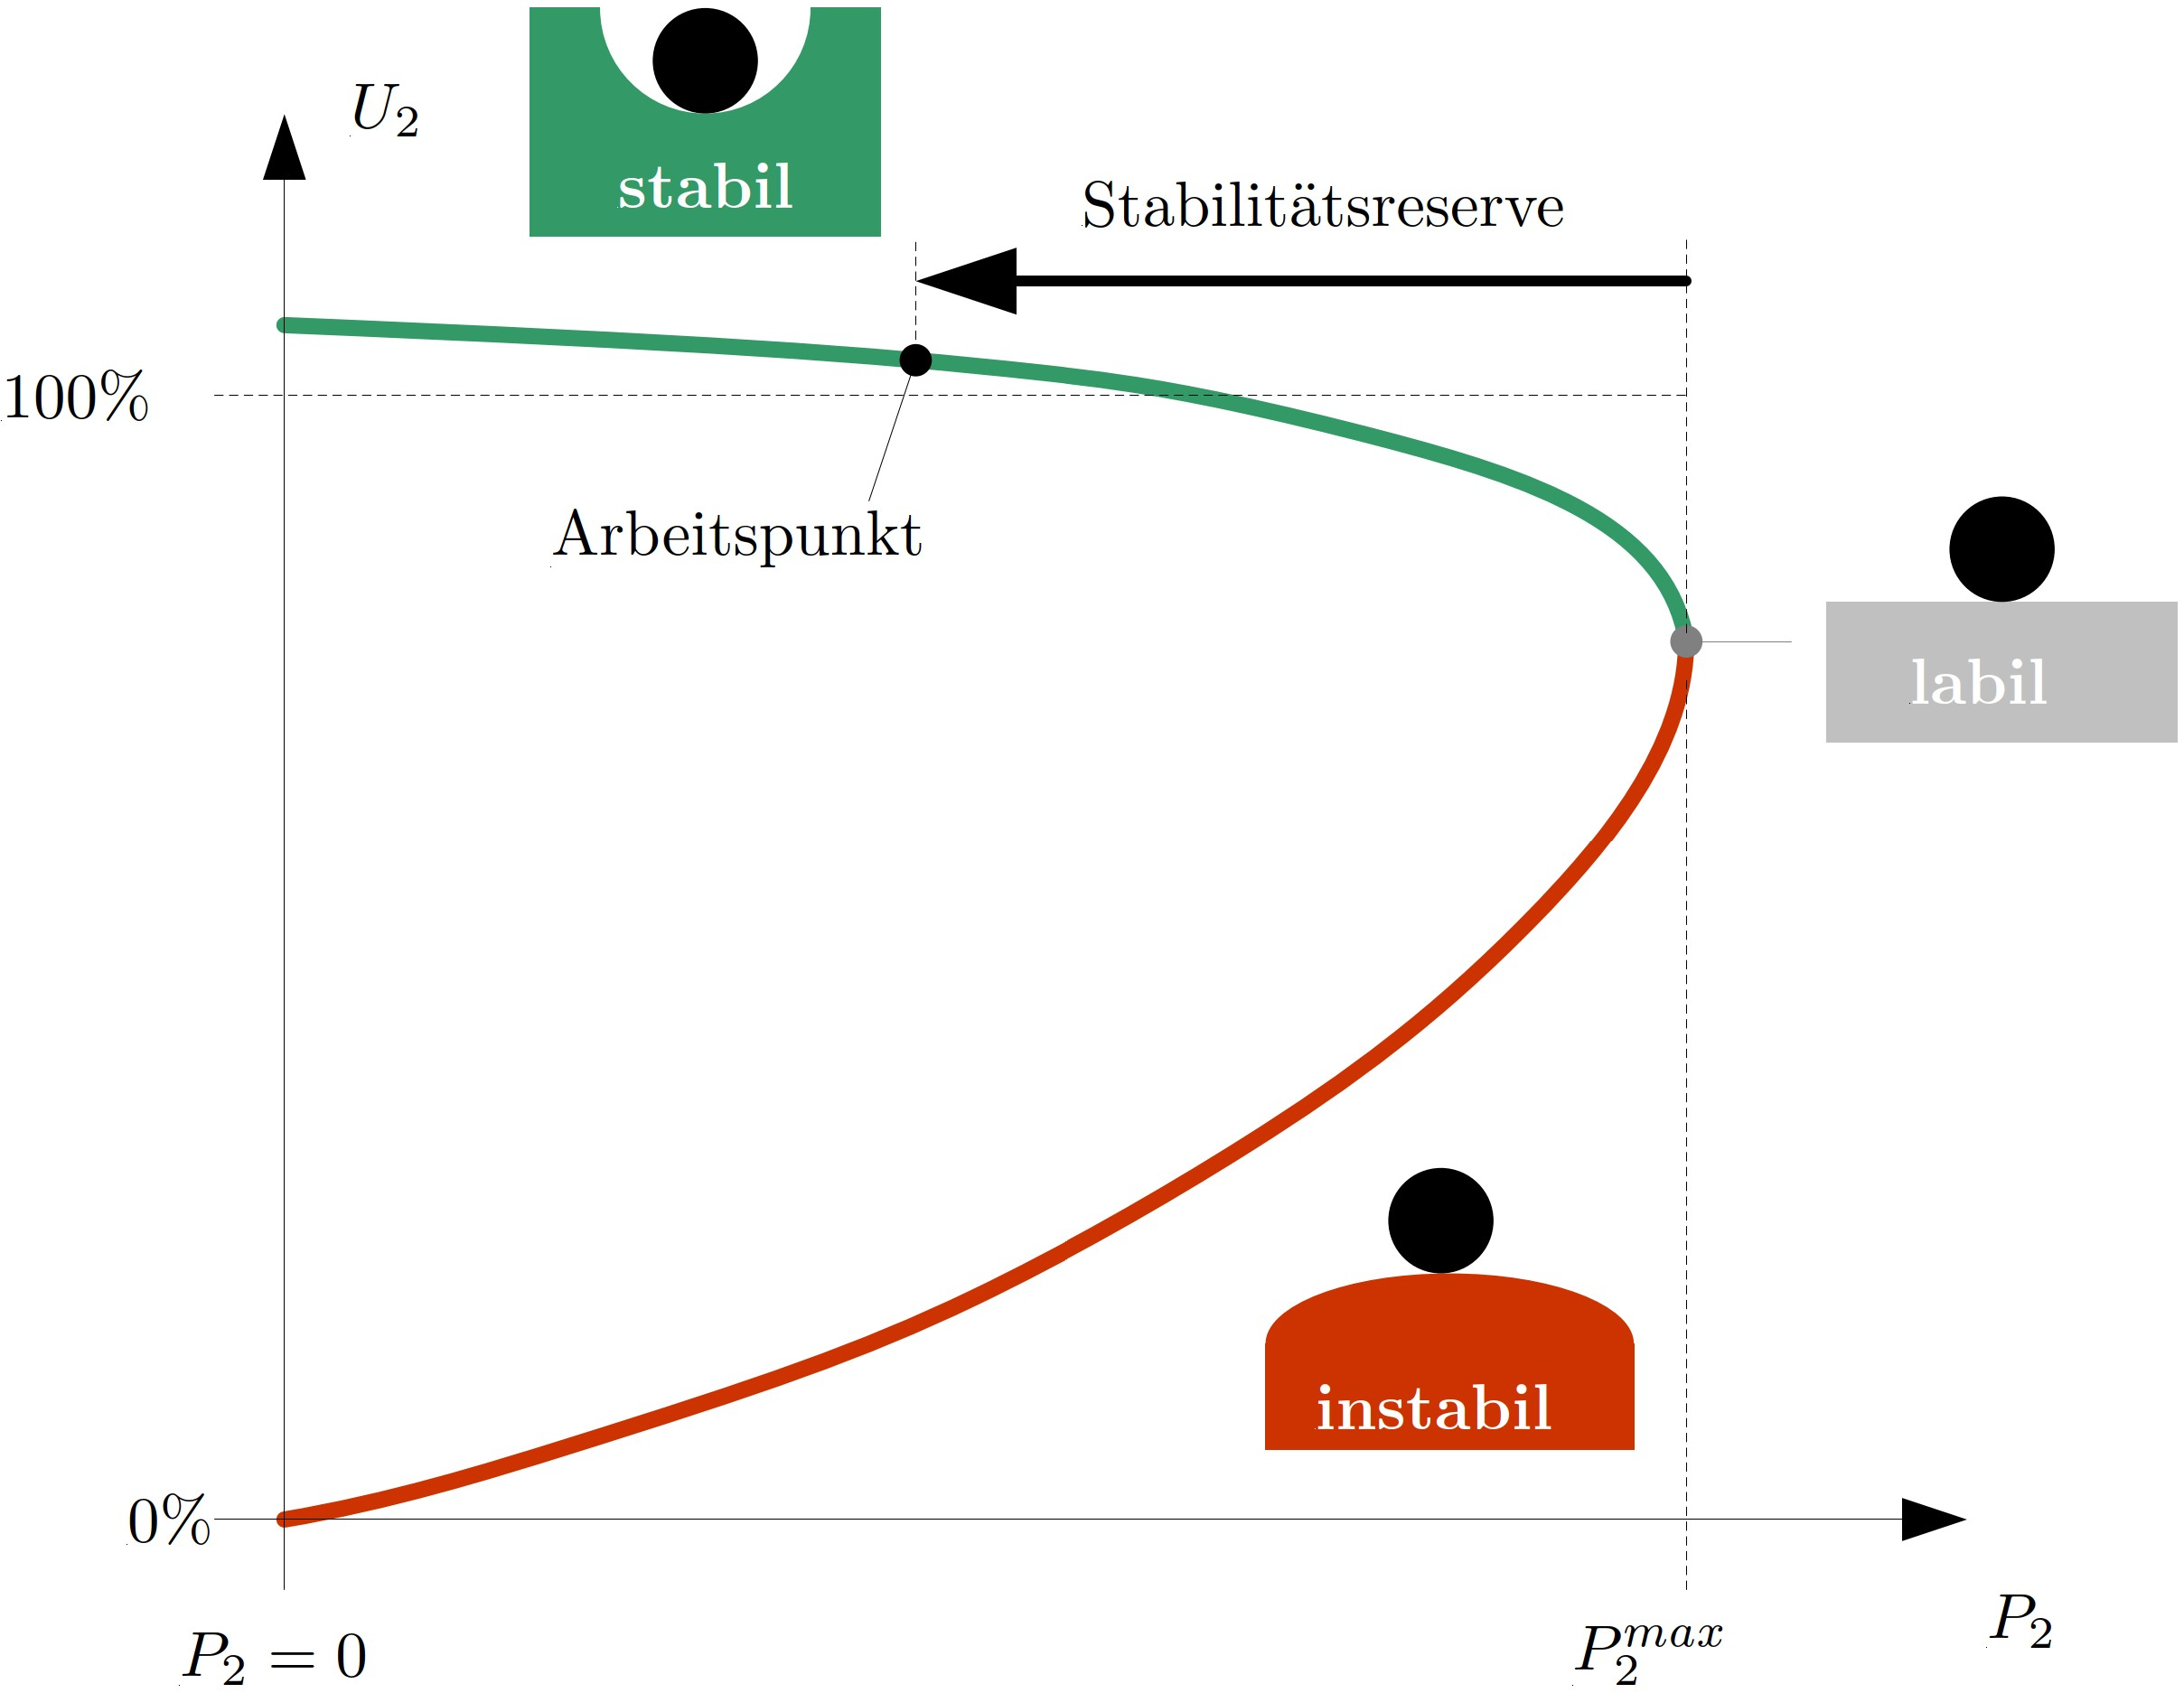
\includegraphics[width=0.98\columnwidth]{images/Spannungsregelung_3.jpg}
        \end{center}    
    \end{minipage}
    \hfill
    \begin{minipage}[c]{0.48\columnwidth}
        \begin{center}
            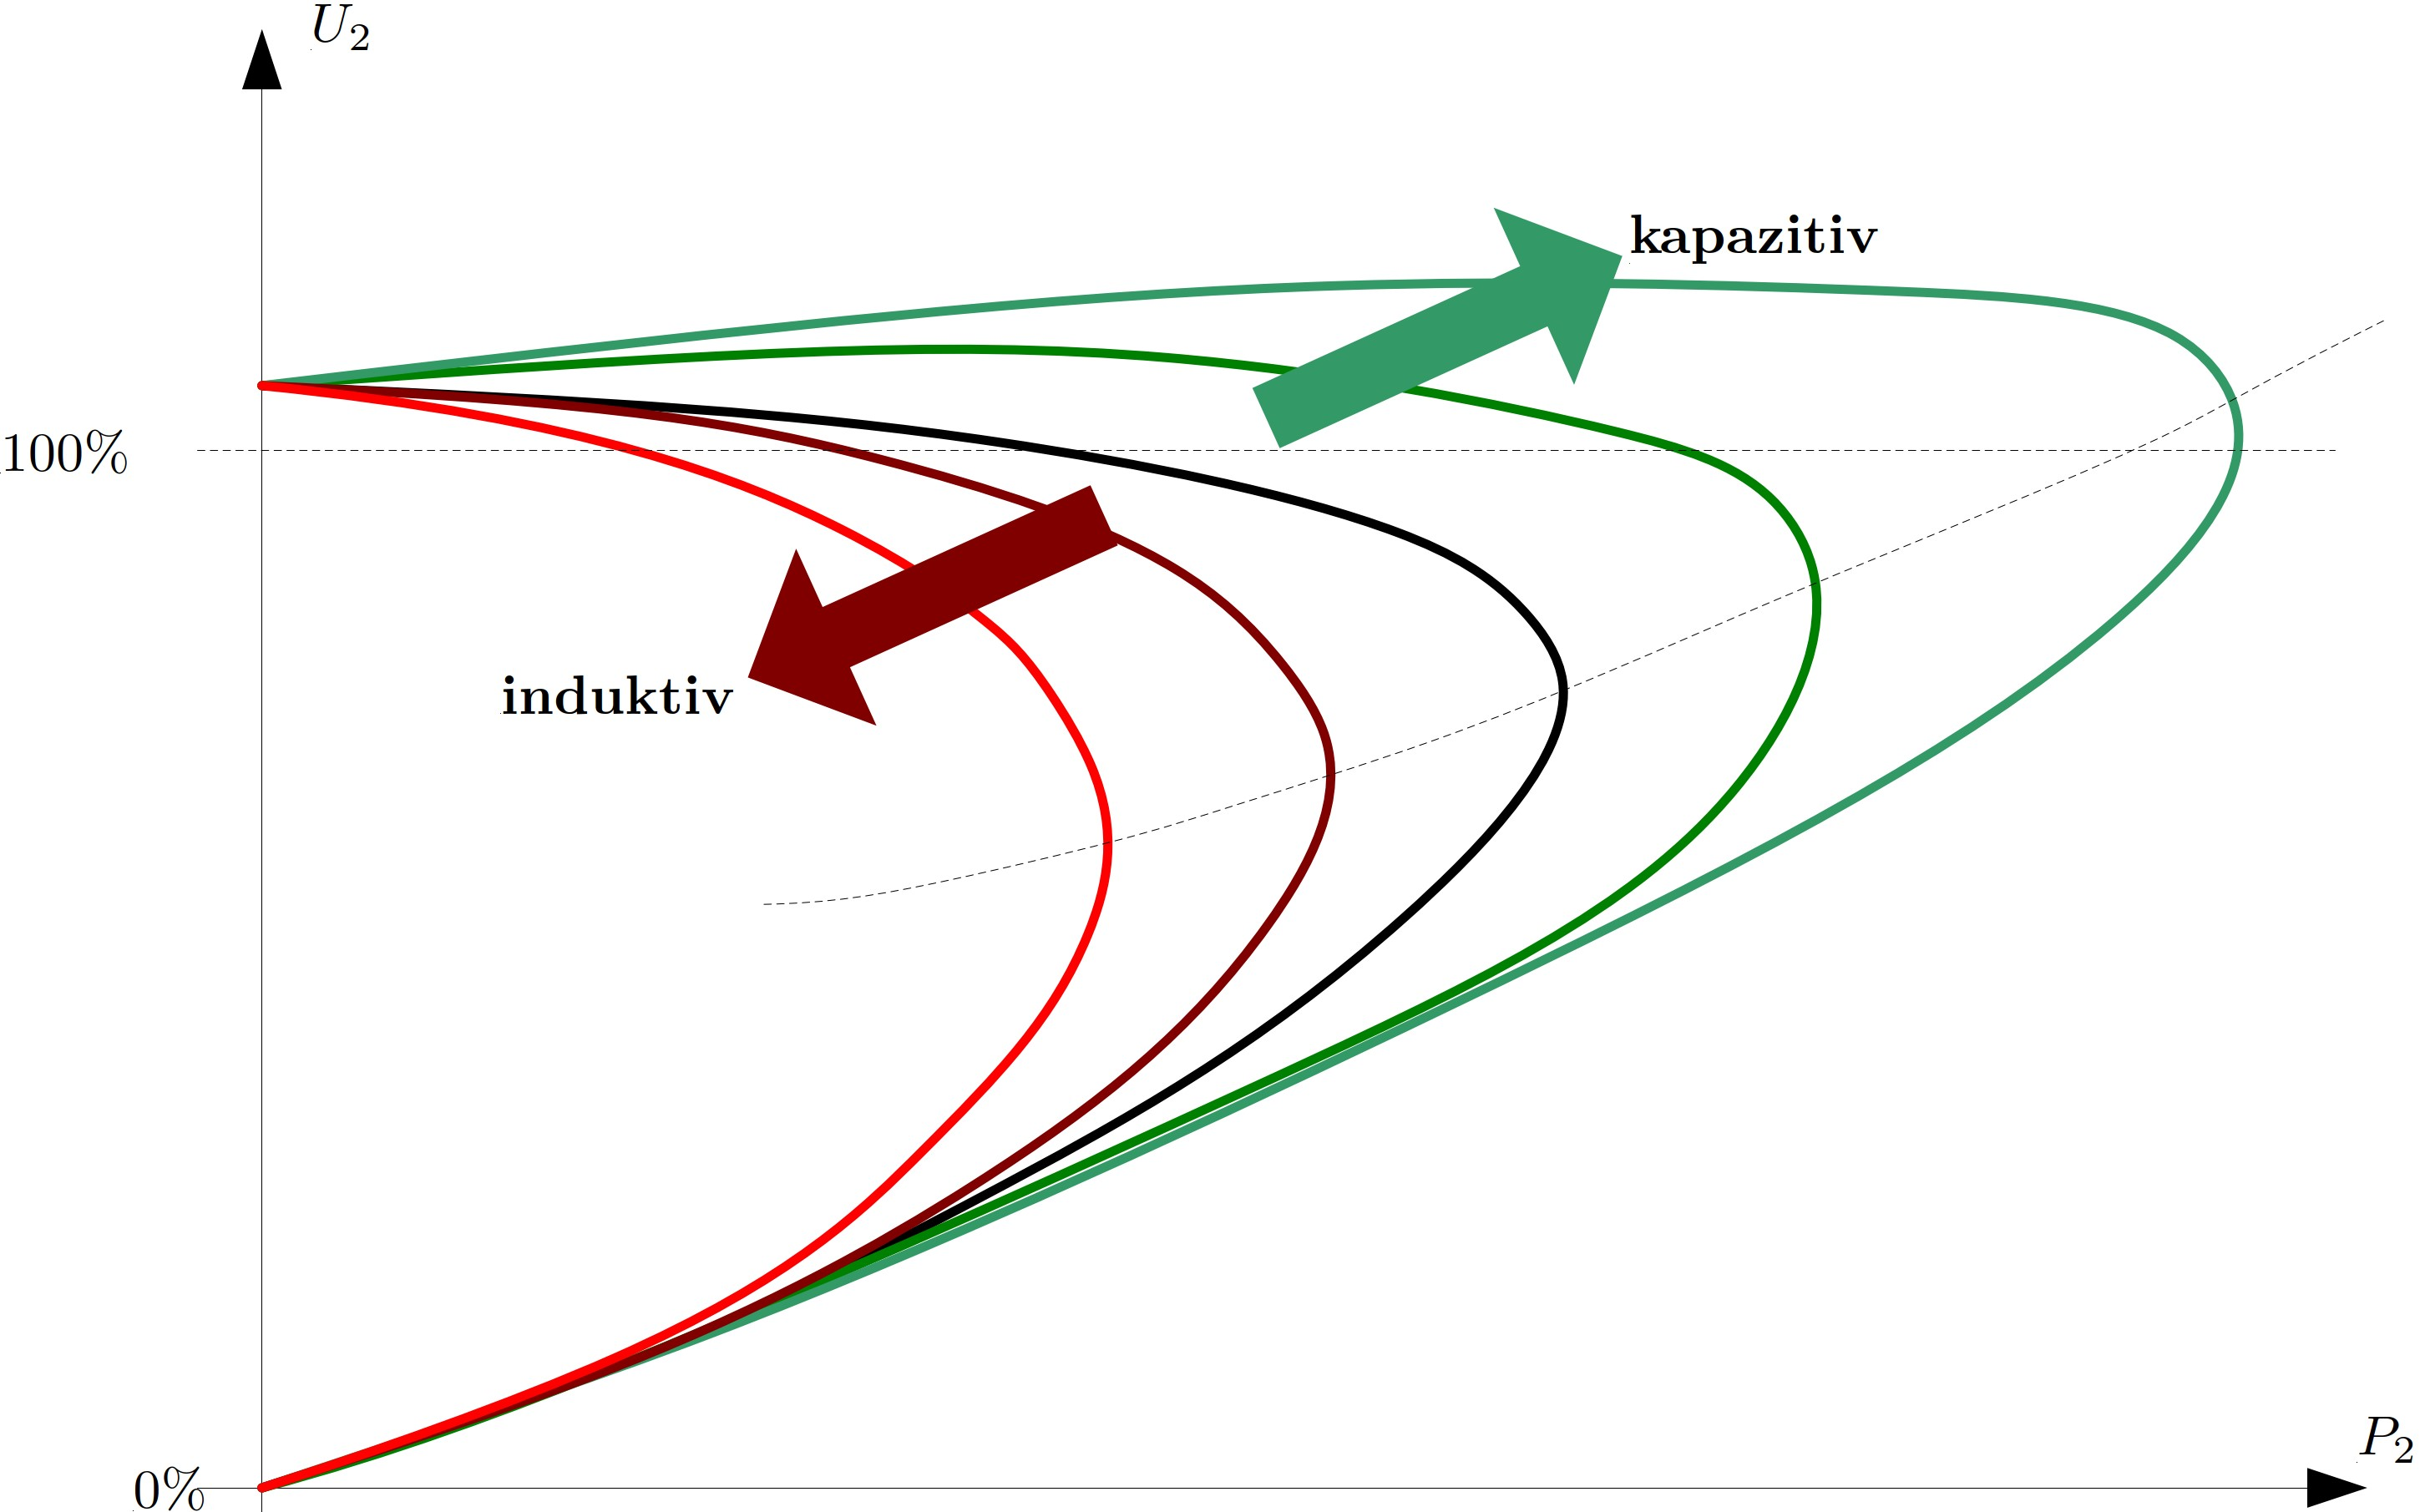
\includegraphics[width=0.98\columnwidth]{images/Spannungsregelung_4.jpg}
        \end{center}
    \end{minipage}

    \vspace{0.3cm}

    \begin{minipage}[c]{0.48\columnwidth}
        \begin{center}
            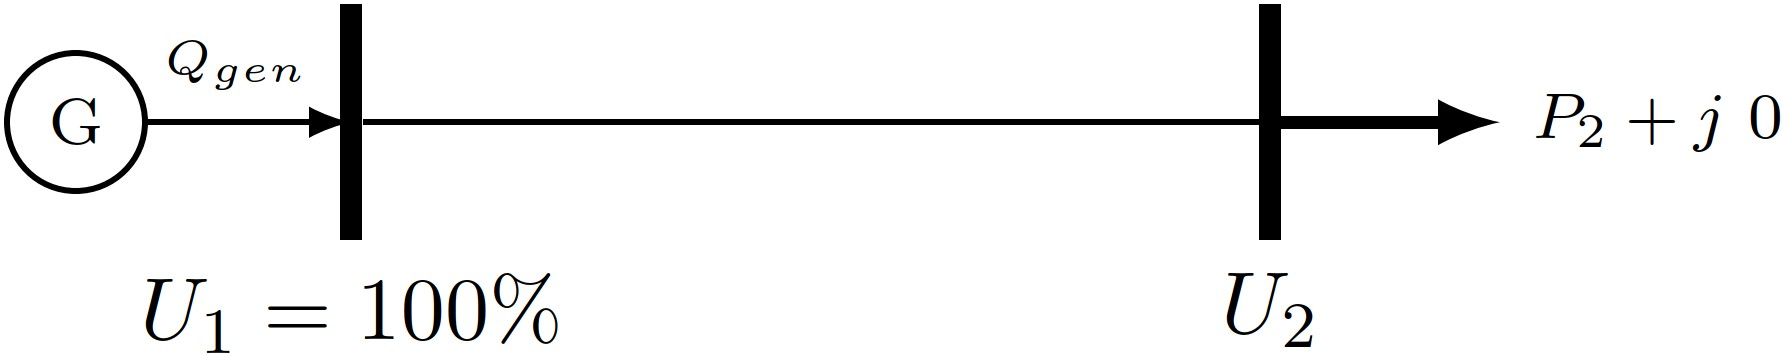
\includegraphics[width=0.98\columnwidth]{images/Spannungsregelung_5.jpg}
        \end{center}    
    \end{minipage}
    \hfill
    \begin{minipage}[c]{0.48\columnwidth}
        \begin{center}
            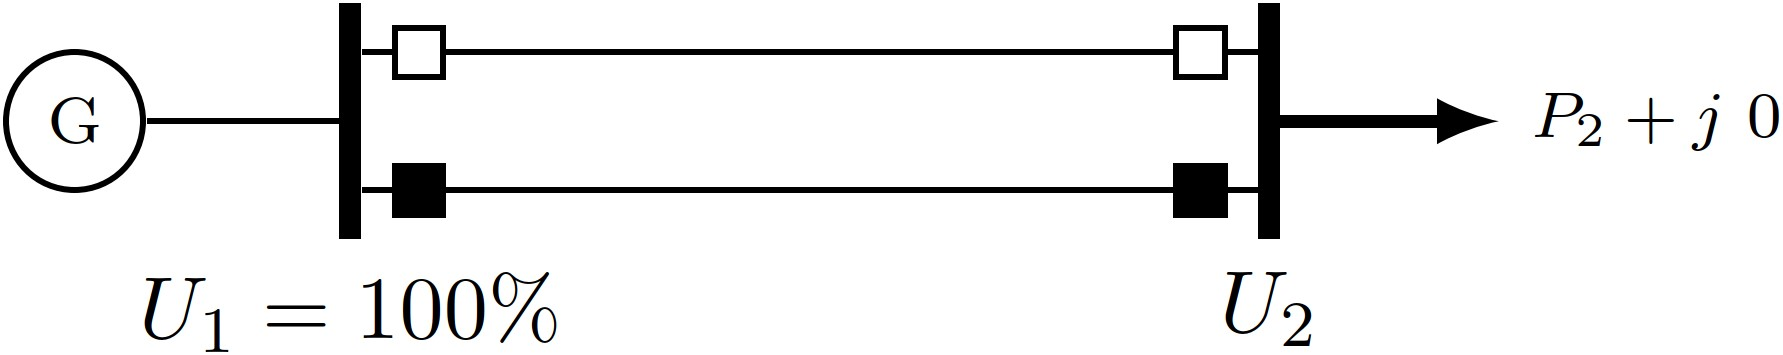
\includegraphics[width=0.98\columnwidth]{images/Spannungsregelung_7.jpg}
        \end{center}
    \end{minipage}

    \vspace{0.1cm}

    \begin{minipage}[c]{0.48\columnwidth}
        \begin{center}
            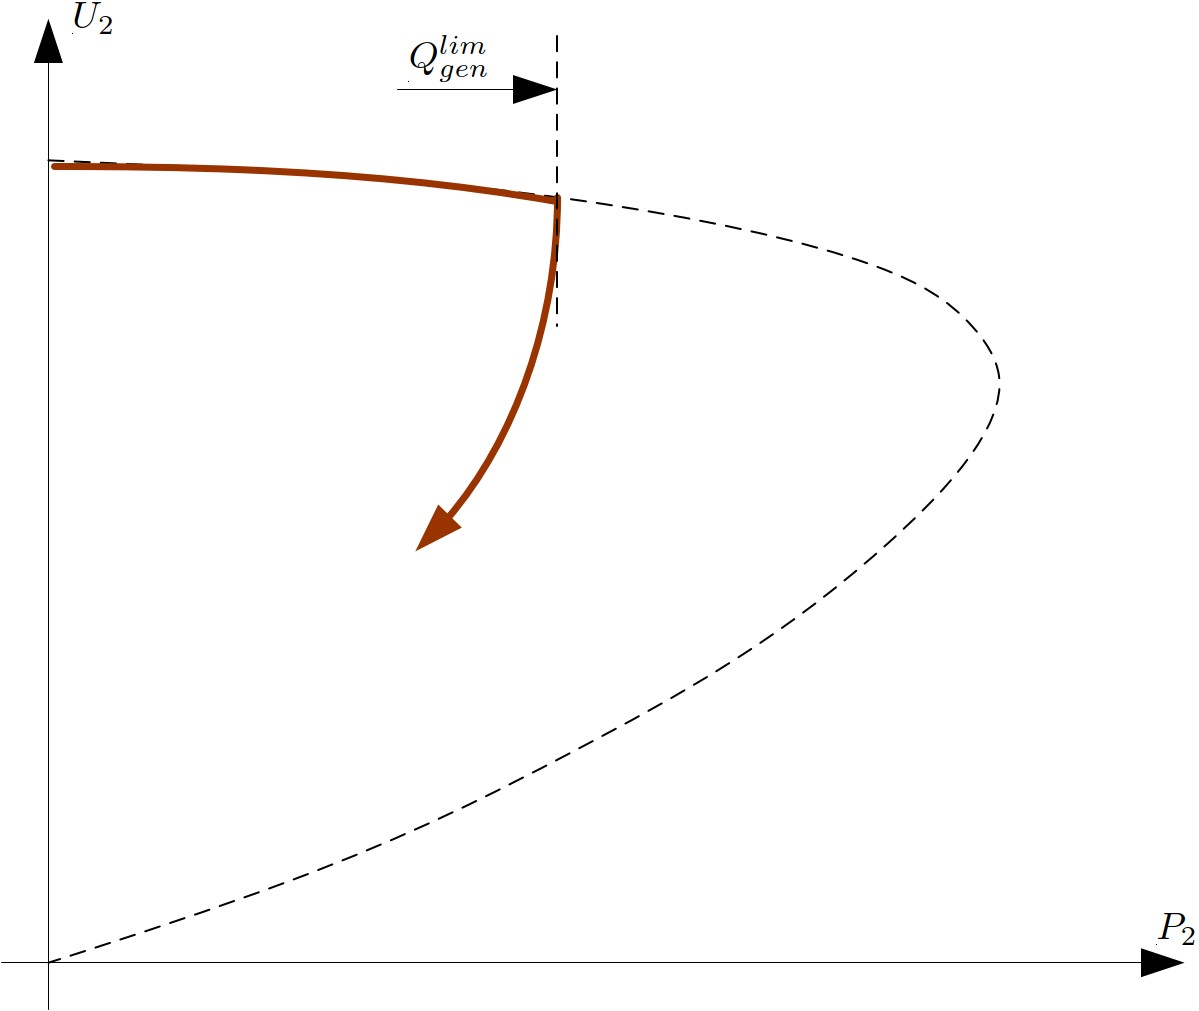
\includegraphics[width=0.9\columnwidth]{images/Spannungsregelung_6.jpg}
        \end{center}    
    \end{minipage}
    \hfill
    \begin{minipage}[c]{0.48\columnwidth}
        \begin{center}
            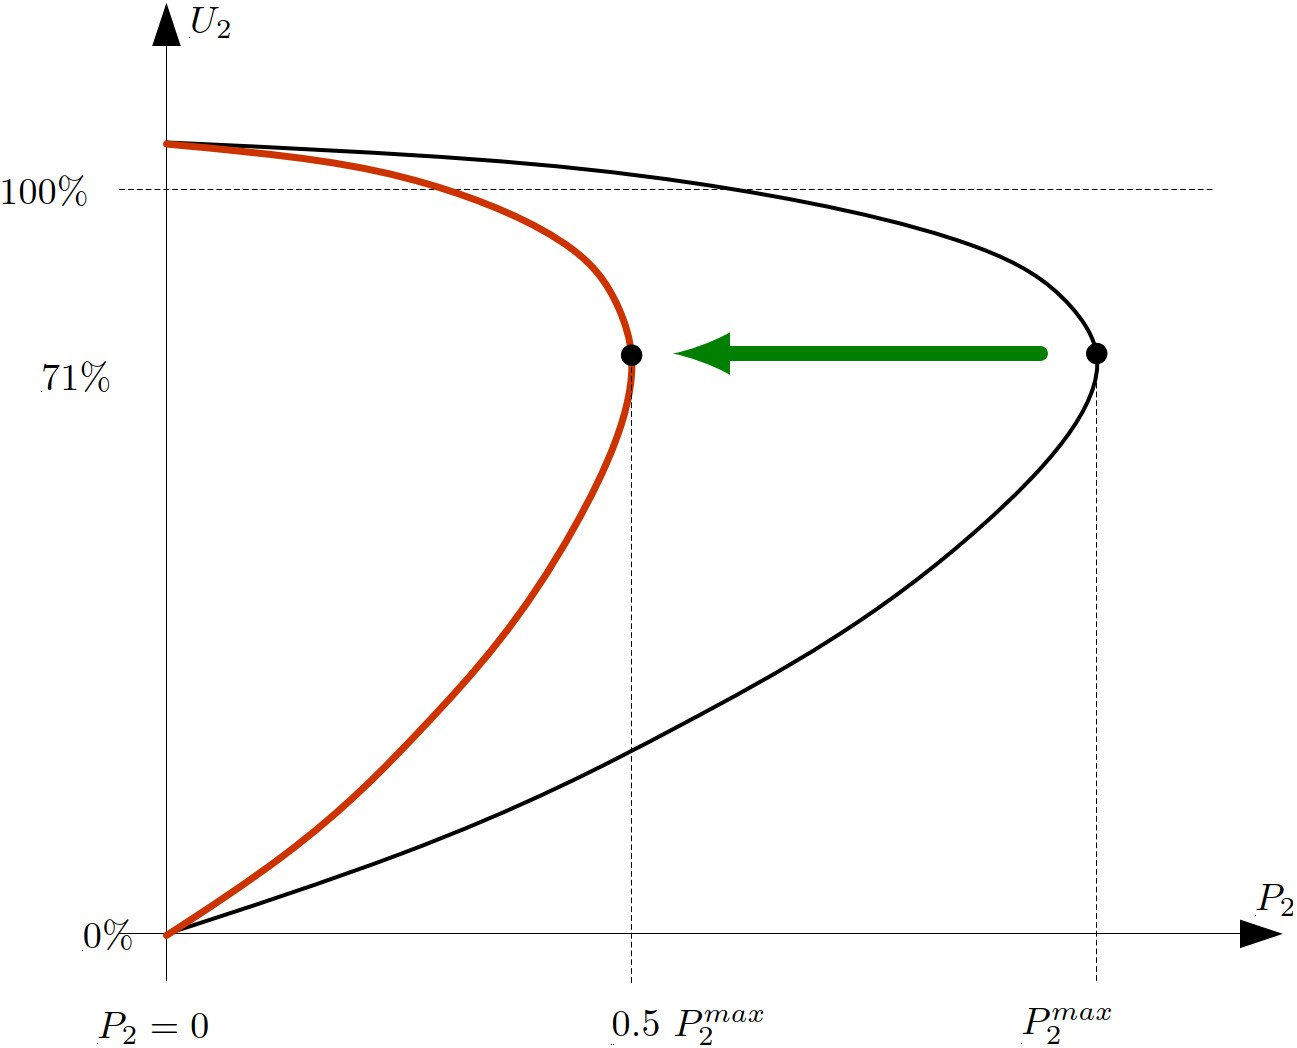
\includegraphics[width=0.9\columnwidth]{images/Spannungsregelung_8.jpg}
        \end{center}
    \end{minipage}

\subsection{Spannungs-Blindleistungs-Regelung}
\subsubsection{Spannungsänderung}
    \begin{minipage}[c]{0.48\columnwidth}
        \begin{center}
            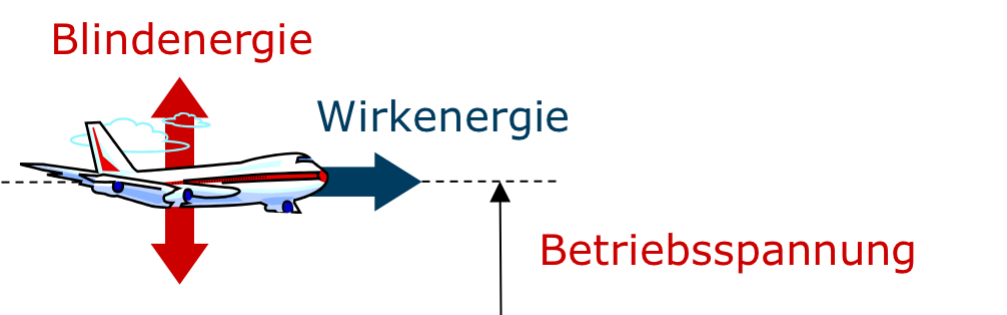
\includegraphics[width=0.98\columnwidth]{images/Spannungs-Blindleistungs-Regelung_1.png}
        \end{center}    
    \end{minipage}
    \hfill
    \begin{minipage}[c]{0.48\columnwidth}
            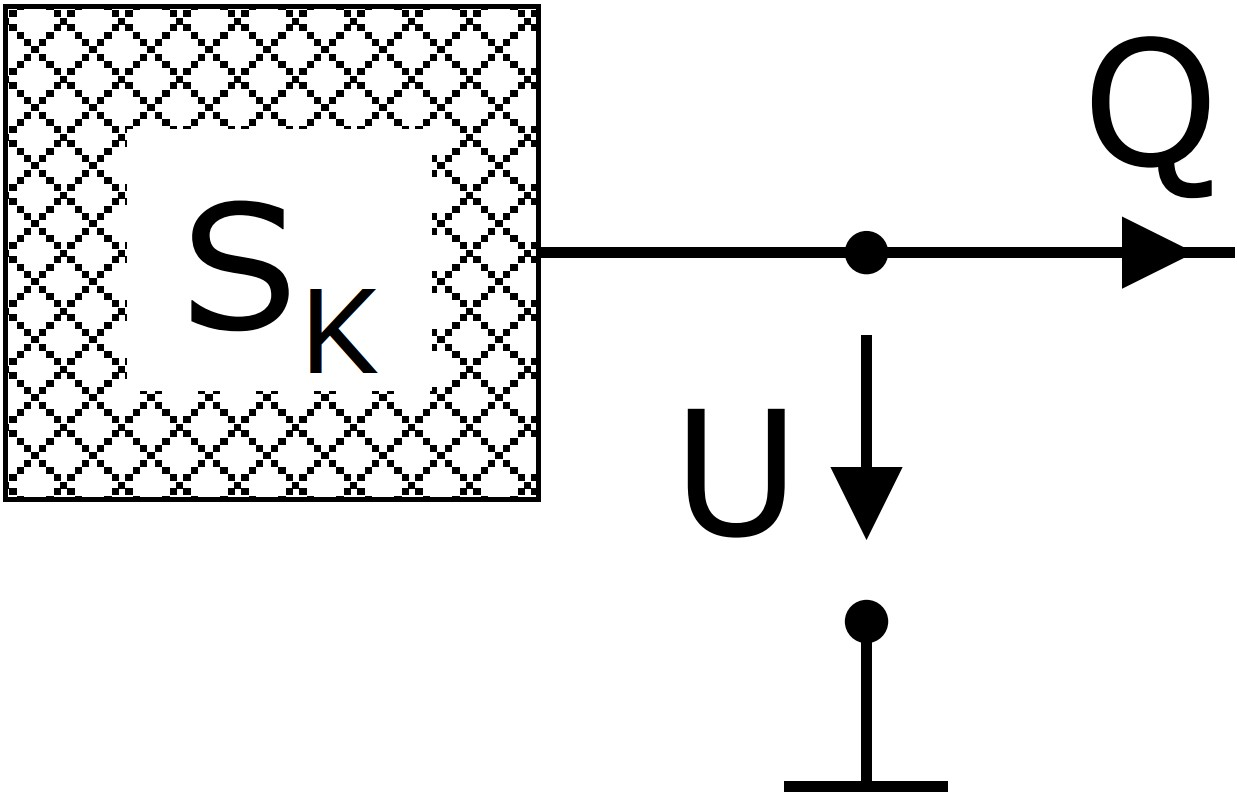
\includegraphics[width=0.5\columnwidth]{images/Spannungs-Blindleistungs-Regelung_2.jpg}
    \end{minipage}

    \begin{minipage}[t]{0.35\columnwidth}
    \centering \vspace{-0.1\baselineskip}
        $\boxed{\Delta U_{\%} = \frac{\Delta Q}{S_K} \cdot 100\%}$
        
        $\boxed{\Delta U = \frac{\Delta Q}{S_K} \cdot U}$
    \end{minipage}%
    \hfill
    \begin{minipage}[t]{0.64\columnwidth}
    \centering \vspace{-0.1\baselineskip}
        \renewcommand{\arraystretch}{1.2}
        \begin{tabular}{@{} l p{4cm} l @{}}
            $[S_K]$  & Kurzschlussleistung \dotfill               & $\text{VA}$ \\
            $[\Delta Q]$ & Veränderung der Blindleistung \dotfill & $\text{VAR}$ \\
            $[U]$ & Referenz-Spannung ($\mathrm{220 \ kV}$ oder $\mathrm{380 \ kV}$) \dotfill & $\mathrm{V}$ \\
            $[\Delta U]$ & Spannungsänderung \dotfill & $\mathrm{V}$ \\
            $[\Delta U_{\%}]$ & Spannungsänderung in Prozent \dotfill & $\%$ \\
        \end{tabular}
    \end{minipage}

    Eine Kapazität speist kapazitive Blindleistung ein, 
    was den Spannungsfall über der Netzimpedanz verringert bzw. 
    kompensiert. Dadurch erhöht sich die Knotenspannung.

\subsubsection{Blindleistung}
    \begin{minipage}[t]{0.49\columnwidth}
        \begin{itemize}
            \item Q-Bilanz eines Netzes ist immer ausgeglichen
            \item Q wirkt unmittelbar und lokal auf U
        \end{itemize}
    \end{minipage}%
    \hfill
    \begin{minipage}[t]{0.49\columnwidth}
        \begin{itemize}
            \item Q fließt von höherer zu tieferer U
            \item Wenn Blindleistung aus dem Netz genommen wird sinkt die Spannung
        \end{itemize}
    \end{minipage}

    \begin{center}
        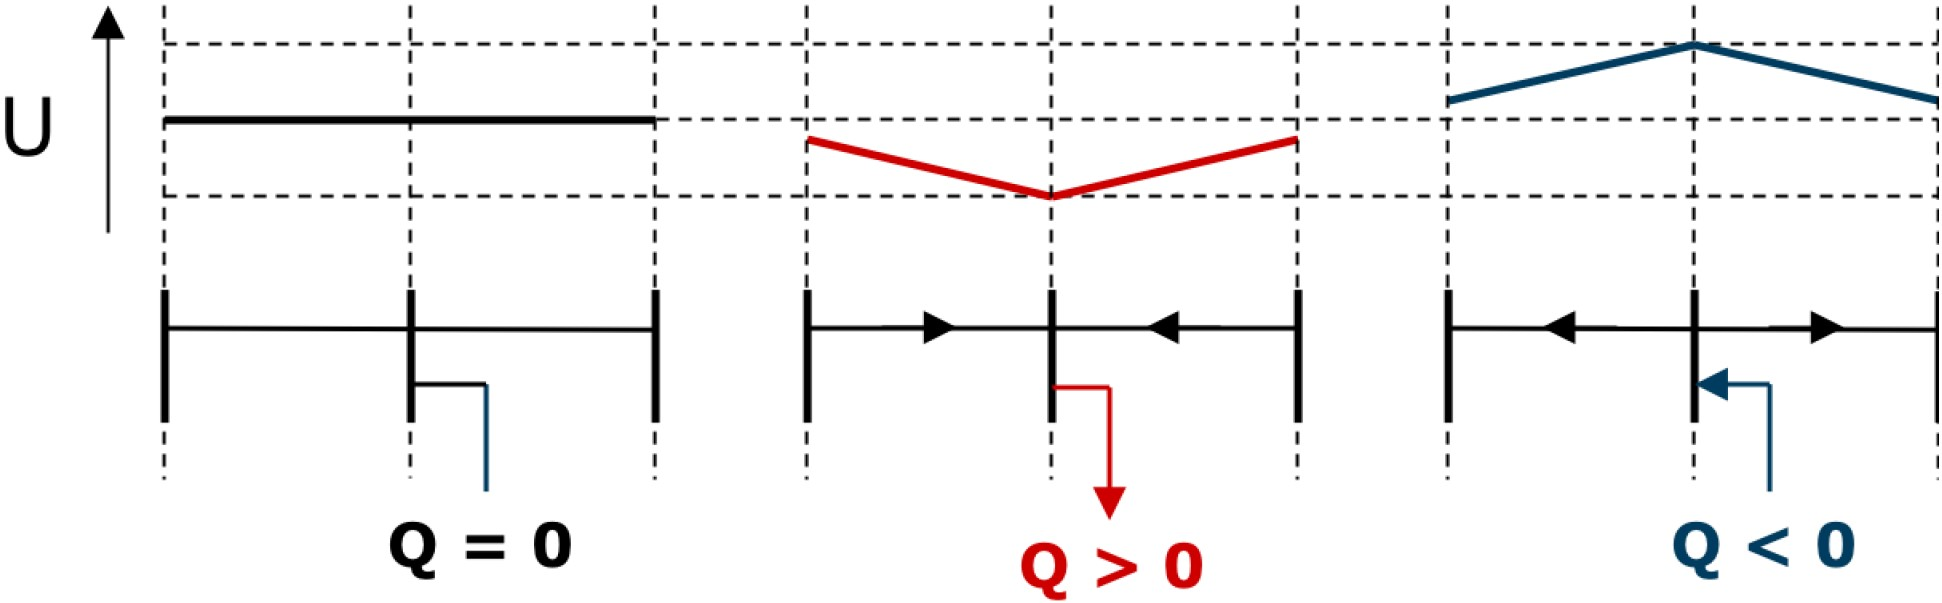
\includegraphics[width=0.7\columnwidth]{images/Spannungs-Blindleistungs-Regelung_3.jpg}\\
    \end{center}

\subsection{Grundlagen Spannungshaltung}
    \begin{center}
        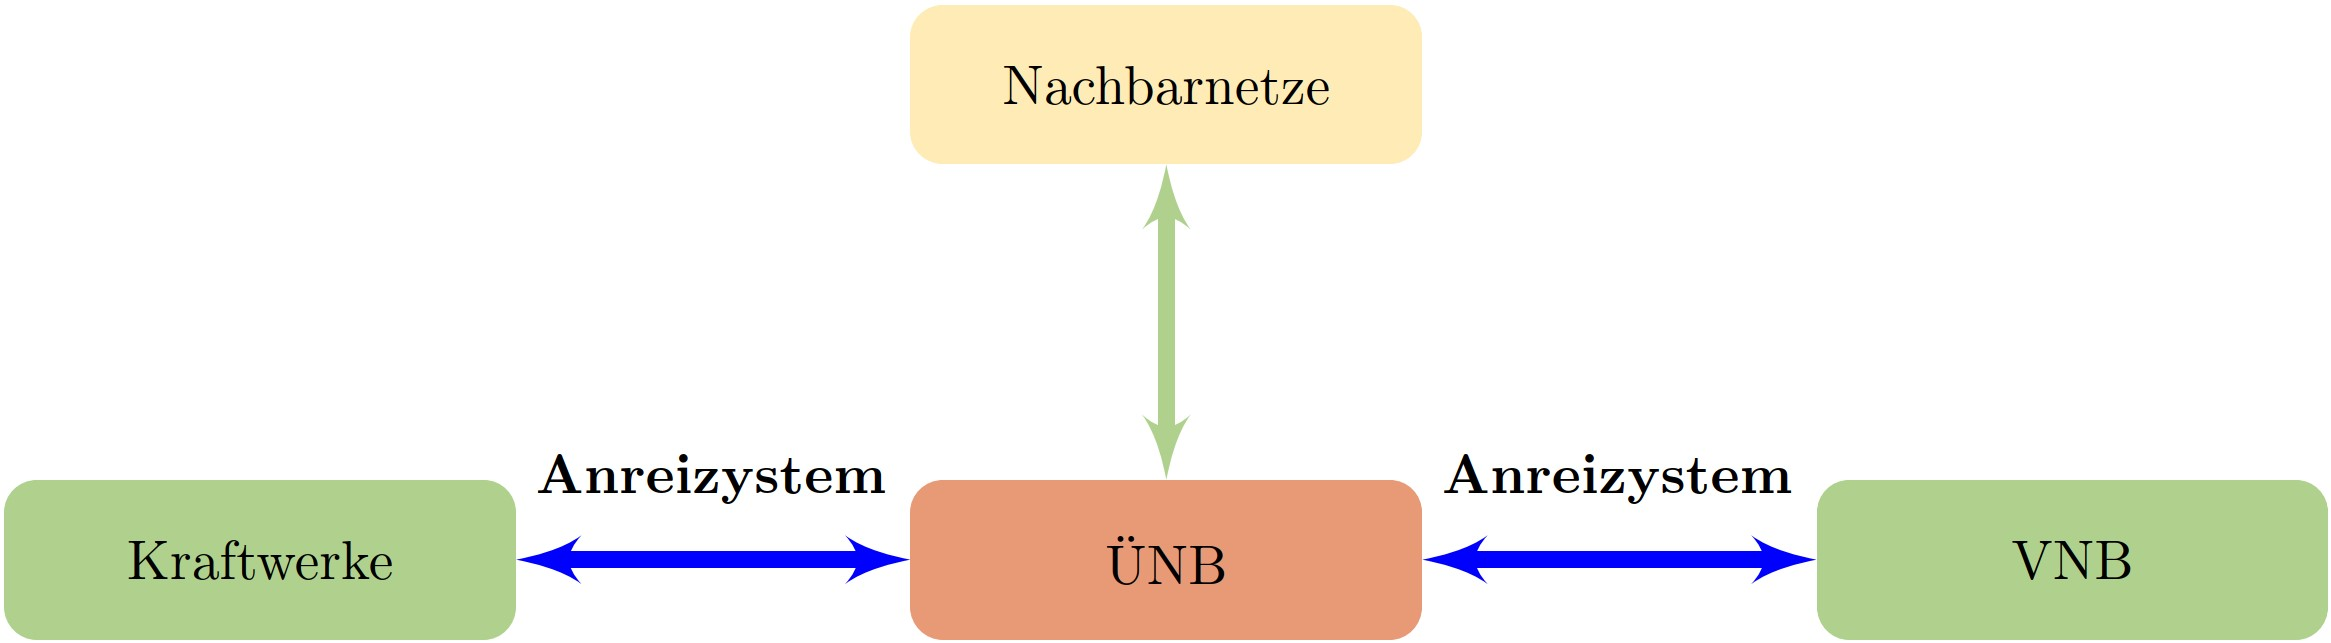
\includegraphics[width=0.9\columnwidth]{images/Grundlagen_Spannungshaltung_1.jpg}
    \end{center}

\subsection{Spannunshaltung in der Schweiz}
    \begin{center}
        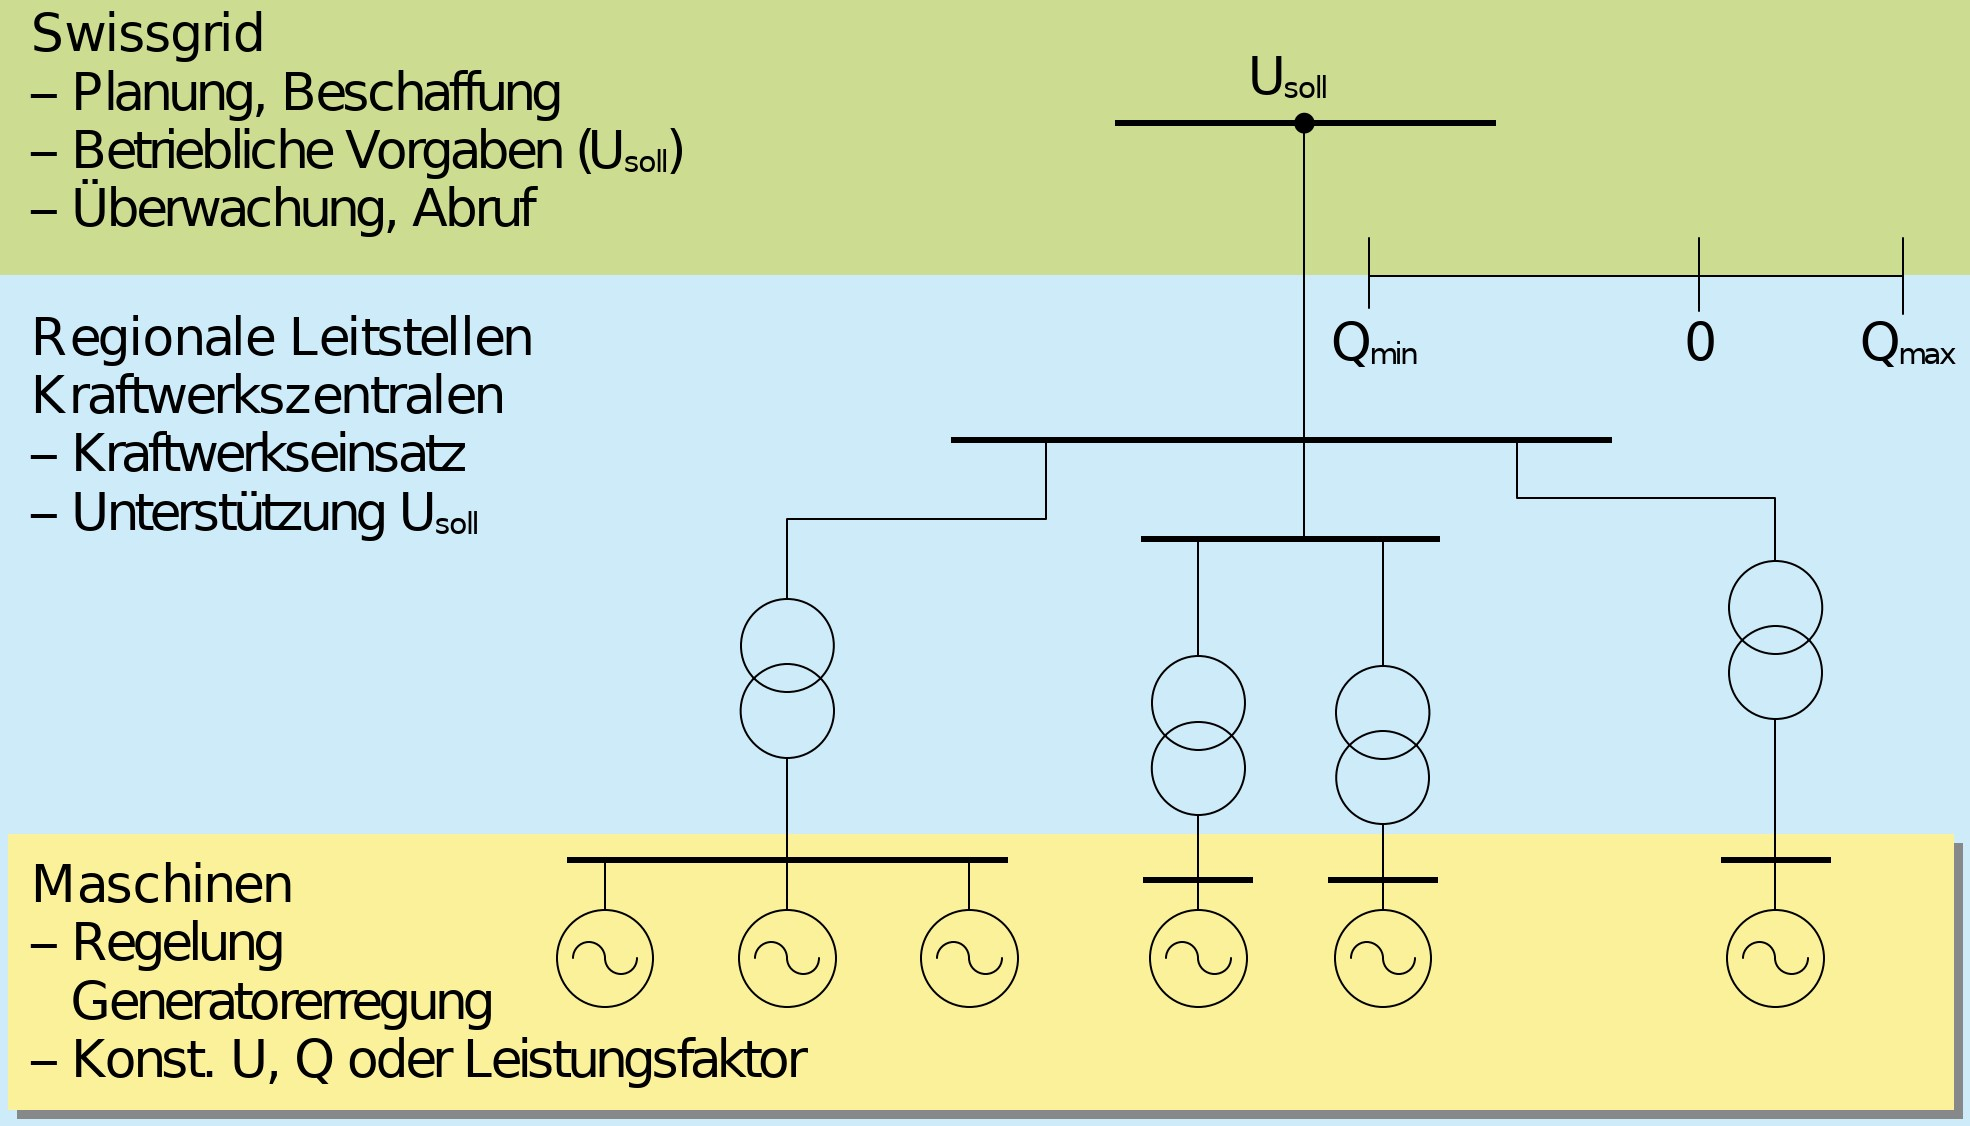
\includegraphics[width=0.9\columnwidth]{images/Spannunshaltung_in_der_Schweiz_1.jpg}
    \end{center}

\subsection{Kraftwerke}
    \begin{itemize}
        \item geregelte Blindleistungsquellen
        \item Vergütung der anforderungskonformen Lieferung von Blindleistung.
    \end{itemize}

    \vspace{0.1cm}

    \begin{minipage}[c]{0.48\columnwidth}
        \begin{center}
            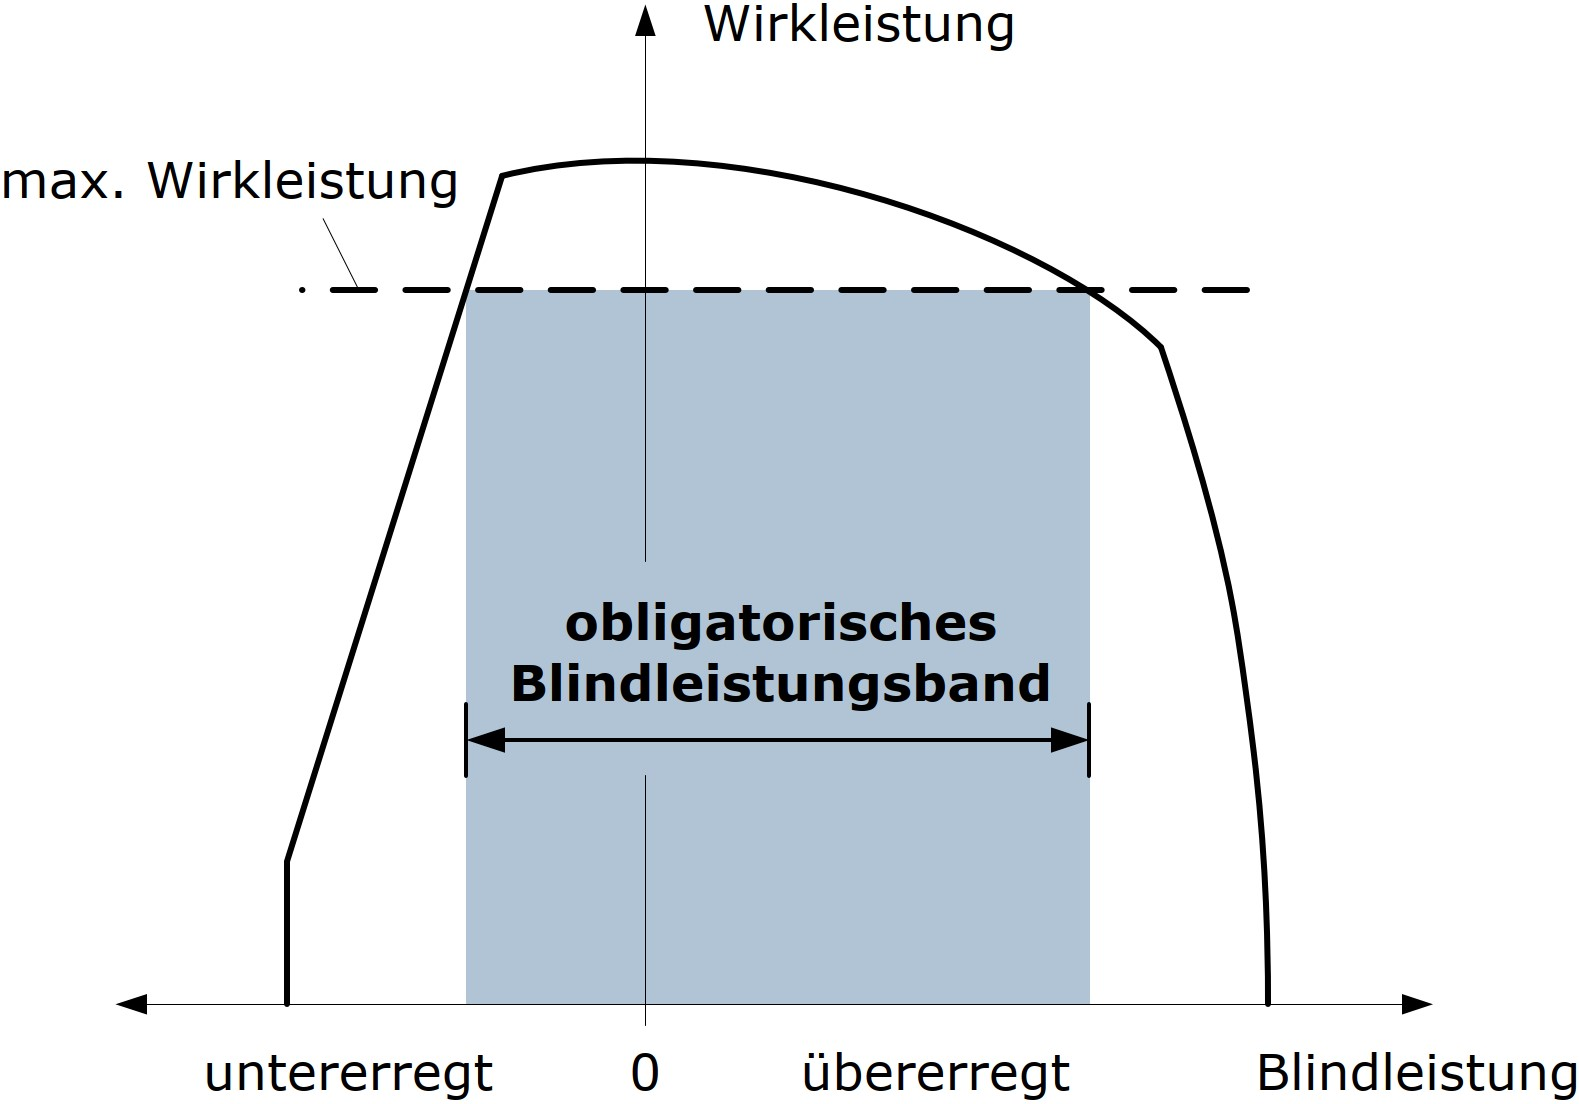
\includegraphics[width=0.95\columnwidth]{images/Kraftwerke_1.jpg}
        \end{center}    
    \end{minipage}
    \hfill
    \begin{minipage}[c]{0.48\columnwidth}
        \begin{center}
            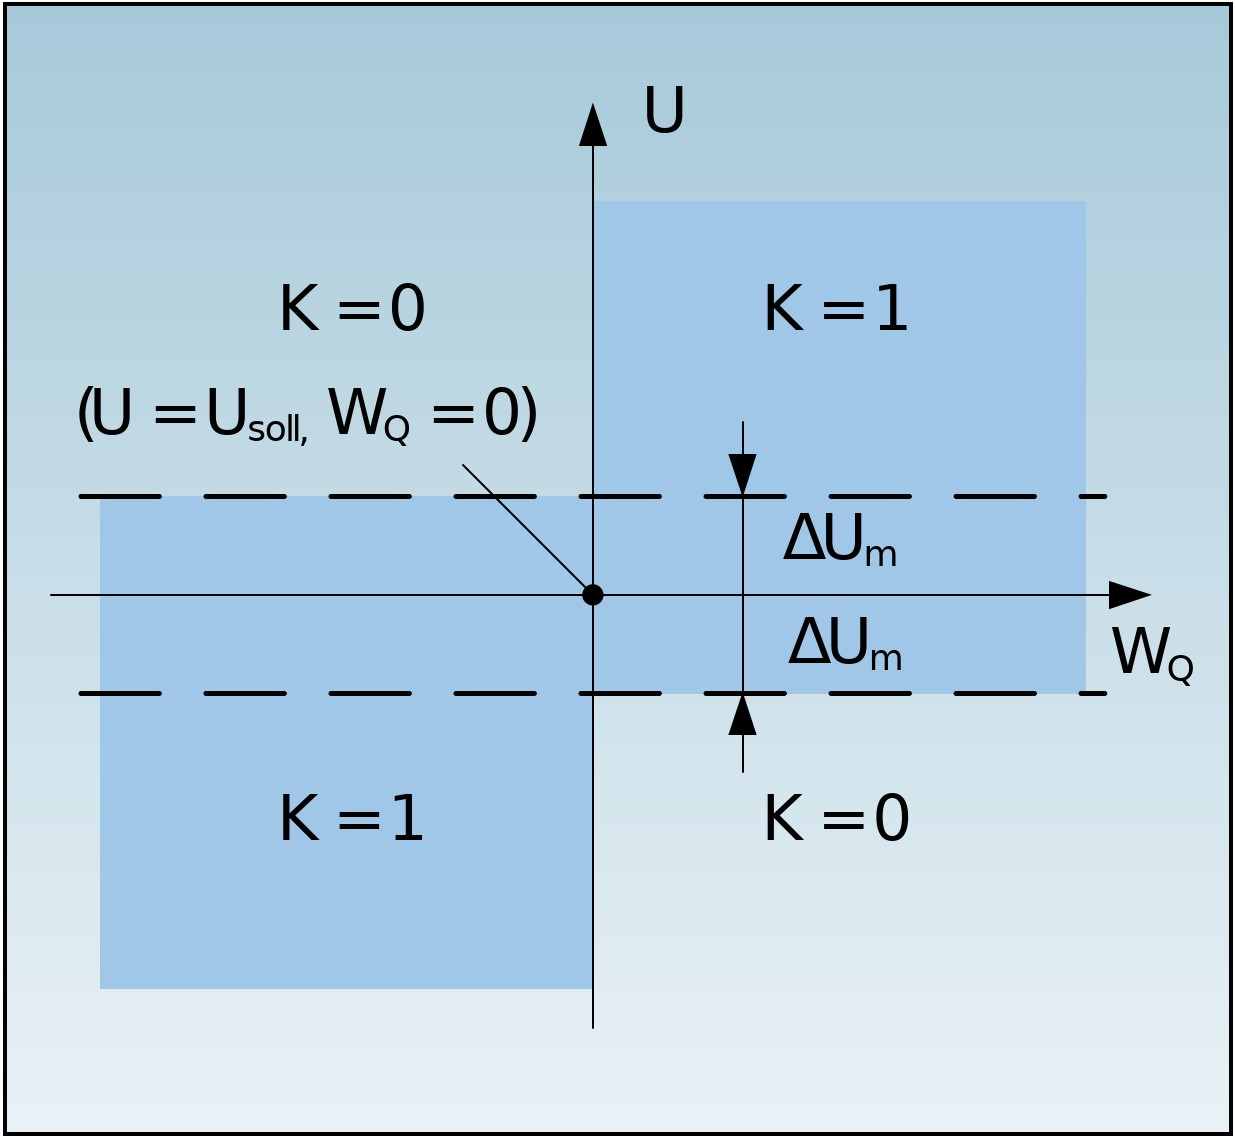
\includegraphics[width=0.8\columnwidth]{images/Kraftwerke_2.jpg}
        \end{center} 
    \end{minipage}

\subsection{Unterlagerte Netze}
    \begin{minipage}[c]{0.38\columnwidth}
        \begin{center}
            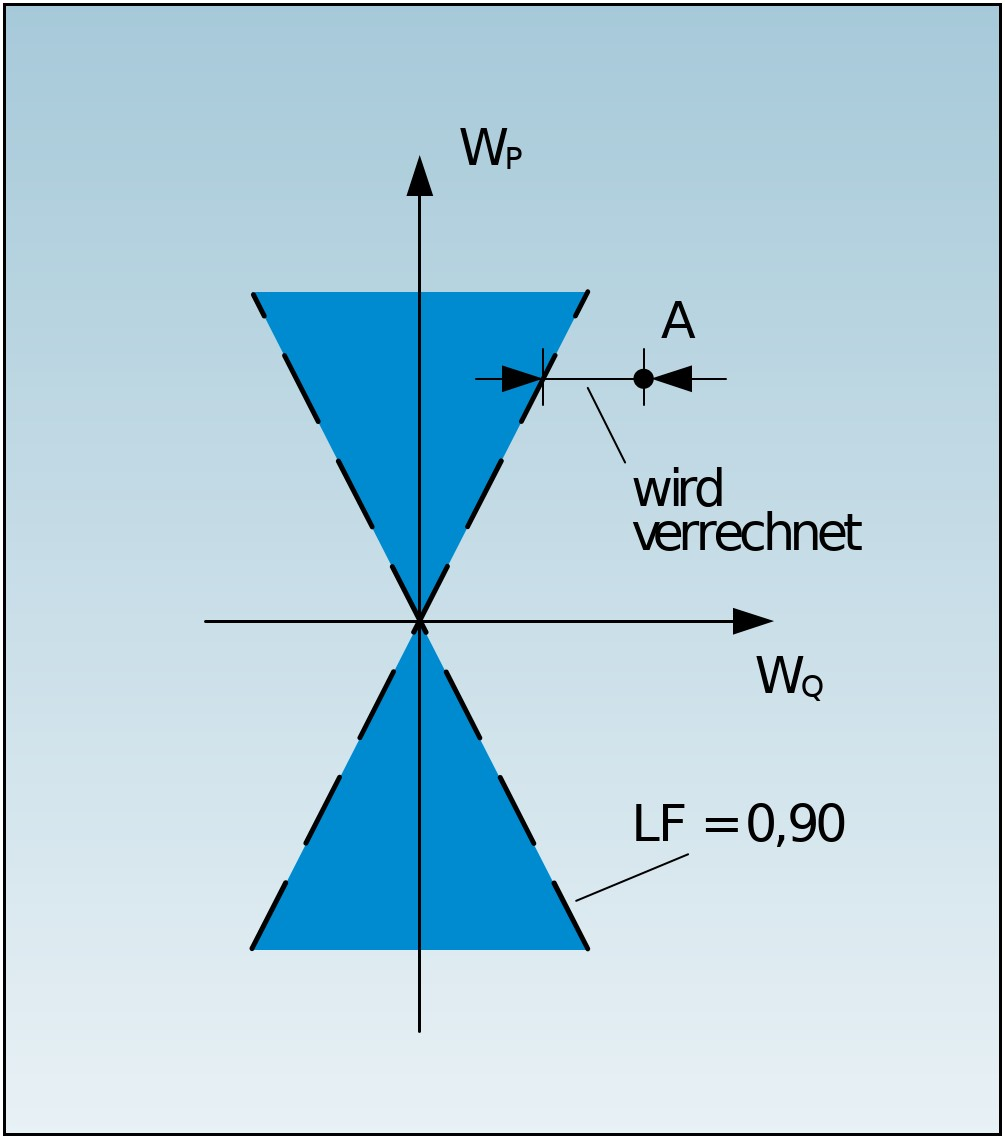
\includegraphics[width=0.98\columnwidth]{images/Unterlagerte_Netze.jpg}
        \end{center}    
    \end{minipage}
    \hfill
    \begin{minipage}[c]{0.58\columnwidth}
        $\boxed{K = \frac{|\Delta U_m|}{|W_Q|} \leq \frac{1}{K_{\text{max}}}}$

        \vspace{0.1cm}
        \renewcommand{\arraystretch}{1.2}
        \begin{tabular}{@{} l p{3cm} l @{}}
            $[W_P]$  & Wirkenergieaustausch     \dotfill    &   $\text{W}$ \\
            $[W_Q]$  & Blindenergieaustausch    \dotfill    &   $\text{var}$ \\
            $[LF]$   & Leistungsfaktor (0{,}9–1)   \dotfill    &   $\text{-}$ \\
            $[\Delta U_m]$ & Spannungsabweichung  \dotfill    &   $\text{kV}$ \\
            $[K]$    & Verhältnis Spannungsabweichung zu Blindenergie \dotfill & $\text{kV}/\text{Mvarh}$
        \end{tabular}

        Für einen Arbeitspunkt A wird die Blindenergie, die der Überschreitung des blauen Bereichs entspricht, in Rechnung gestellt.
    \end{minipage} % done
    \end{layout}
\end{document}
